% UC Berkeley PhD Thesis
% Author: Krish Desai
% Title: Machine Learning Methods for Cross Section Measurements

\documentclass{ucbthesis}

% Load all packages and settings from external file
% thesis-preamble.tex
\setlrmarginsandblock{1in}{1in}{*}
\setulmarginsandblock{1.5in}{1.5in}{*}
\checkandfixthelayout
% ============================================================================
% ENCODING AND FONTS
% ============================================================================
\usepackage[utf8]{inputenc}
\usepackage[T1]{fontenc}

% ============================================================================
% DOCUMENT LAYOUT AND TYPOGRAPHY
% ============================================================================
\usepackage{geometry}
\usepackage[english]{babel}
\usepackage{csquotes}

% Microtype for better typography
\usepackage
% [protrusion=false, expansion=true, factor=1100, final, 
%             tracking=true, kerning=true, spacing=true, 
%             babel=true]
            {microtype}
\microtypecontext{spacing=nonfrench}
\SetExtraKerning[unit=space]
    {encoding={*}, family={bch}, series={*}, size={footnotesize,small,normalsize}}
    {\textendash={800,800},
     "28={ ,150},
     "29={150, },
     \textquotedblleft={ ,150},
     \textquotedblright={150, }}
\SetTracking{encoding={*}, shape=sc}{40}
\microtypesetup{protrusion=false}

%============================================================================
% MATHEMATICS PACKAGES
% ============================================================================
\usepackage{amsmath}
\usepackage{amssymb}
\usepackage{amsthm}
\usepackage{nicefrac}
\usepackage{mathtools}
%============================================================================
% GRAPHICS AND VISUAL ELEMENTS
% ============================================================================
\usepackage{graphicx}
\usepackage{subcaption}
\usepackage{tabularx}
\usepackage{booktabs}
\usepackage{multirow}
\usepackage{array}
\usepackage{xcolor}

% ============================================================================
% ALGORITHMS AND CODE
% ============================================================================
\usepackage[ruled,vlined]{algorithm2e}
\usepackage{listings} % For code listings if needed

% ============================================================================
% BIBLIOGRAPHY
% ============================================================================
\usepackage[
    backend=biber,
    style=numeric-comp,
    sorting=none,
    maxbibnames=99,
    giveninits=true
]{biblatex}
\addbibresource{references.bib}
% Ensure bibliography is printed and proper backend is used
\AtEndDocument{\printbibliography}

% ============================================================================
% HYPERLINKS AND CROSS-REFERENCES
% ============================================================================

\usepackage[
    hidelinks,
    pdfusetitle,
    bookmarks=true,
    bookmarksnumbered=true,
    bookmarksopen=true,
    bookmarksopenlevel=1,
    breaklinks=true,
    pdfborder={0 0 0},
    colorlinks=false
]{hyperref}
\usepackage{url}
\usepackage[capitalise,noabbrev]{cleveref}
\crefname{equation}{Eq.}{Eqs.}
\crefname{figure}{Fig.}{Figs.}
\crefname{table}{Table}{Tables}
\crefname{section}{Section}{Sections}
\crefname{chapter}{Chapter}{Chapters}
\crefname{paragraph}{Section}{Sections}
\crefname{subparagraph}{Section}{Sections}

% ============================================================================
% UTILITIES
% ============================================================================
\usepackage{pgffor}
\usepackage{appendix}
\usepackage{enumitem} % Better list environments
\usepackage{siunitx}
\usepackage{xparse}
\NewCommandCopy\siqty\qty
\usepackage{comment} % Block comments
\usepackage{physics} % MUST BE LOADED AFTER SIUNITX


% 
%============================================================================
% CUSTOM COLORS
% ============================================================================
\definecolor{darkred}{rgb}{1.0,0.1,0.1}
\definecolor{darkgreen}{rgb}{0.1,0.7,0.1}
\definecolor{darkblue}{rgb}{0.1,0.1,0.7}
\definecolor{commentcolor}{rgb}{0.5,0.5,0.5}

% ============================================================================
% EDITORIAL COMMANDS
% ============================================================================
% For draft versions - remove or comment out for final version
\newcommand{\kd}[1]{\textbf{\color{darkred}[#1 --KD]}}
\newcommand{\bn}[1]{\textbf{\color{darkgreen}[#1 --BN]}}
\newcommand{\todo}[1]{\textbf{\color{darkblue}[TODO: #1]}}
\newcommand{\note}[1]{\textbf{\color{commentcolor}[Note: #1]}}

% For final version, uncomment these to remove all editorial marks:
% \renewcommand{\kd}[1]{}
% \renewcommand{\bn}[1]{}
% \renewcommand{\todo}[1]{}
% \renewcommand{\note}[1]{}

% ============================================================================
% MATHEMATICAL NOTATION
% ============================================================================
% Common operators
\DeclareMathOperator*{\argmax}{arg\,max}
\DeclareMathOperator*{\argmin}{arg\,min}
\DeclareMathOperator{\E}{\mathbb{E}}
\DeclareMathOperator{\Var}{Var}
\DeclareMathOperator{\Cov}{Cov}

% Shortcuts
\newcommand{\inv}{^{-1}}
\newcommand{\R}{\mathbb{R}}
\newcommand{\N}{\mathbb{N}}
\newcommand{\Z}{\mathbb{Z}}
\newcommand{\C}{\mathbb{C}}
\newcommand{\qt}{\widetilde{q}}

% Vectors and matrices
\renewcommand{\vec}[1]{\boldsymbol{#1}}
\newcommand{\mat}[1]{\boldsymbol{#1}}

% Probability
\newcommand{\prob}[1]{\mathbb{P}\left(#1\right)}
\newcommand{\expect}[1]{\mathbb{E}\left[#1\right]}

% ============================================================================
% THEOREM ENVIRONMENTS
% ============================================================================
\theoremstyle{definition}
\newtheorem{theorem}{Theorem}[chapter]
\newtheorem{lemma}[theorem]{Lemma}
\newtheorem{proposition}[theorem]{Proposition}
\newtheorem{corollary}[theorem]{Corollary}
\newtheorem{definition}[theorem]{Definition}
\newtheorem{example}[theorem]{Example}

% ============================================================================
% CUSTOM ENVIRONMENTS
% ============================================================================
% Shorthand for equations (use with caution)
\renewcommand{\[}{\begin{equation}}
\renewcommand{\]}{\end{equation}}

% Column type for math mode in tables
\newcolumntype{M}{>{\(\displaystyle}c<{\)}}

% ============================================================================
% DOCUMENT SETTINGS
% ============================================================================
% Paragraph indentation
\usepackage{indentfirst}
% Double spacing
\def\dsp{\def\baselinestretch{2.0}\large\normalsize}
\dsp

% Caption formatting
\addtolength{\abovecaptionskip}{\baselineskip}

% Prevent widows and orphans
\widowpenalty=10000
\clubpenalty=10000

% Float placement
\renewcommand{\topfraction}{0.85}
\renewcommand{\bottomfraction}{0.85}
\renewcommand{\textfraction}{0.1}
\renewcommand{\floatpagefraction}{0.85}

\setcounter{secnumdepth}{6}
\setcounter{tocdepth}{6}
\renewcommand{\thechapter}{\Roman{chapter}}
\renewcommand{\thesection}{\thechapter.\Alph{section}}
\renewcommand{\thesubsection}{\thesection.\arabic{subsection}}
\renewcommand{\thesubsubsection}{\thesubsection.\roman{subsubsection}}
\renewcommand{\theparagraph}{\thesubsubsection.\alph{paragraph}}
\renewcommand{\thesubparagraph}{\theparagraph.\oldstylenums{\arabic{subparagraph}}}


% ============================================================================
% BEGIN DOCUMENT
% ============================================================================
\includeonly{chapters/05-moment-unfolding}
\begin{document}

% ============================================================================
% METADATA
% ============================================================================
\title{Machine Learning Methods for Cross Section Measurements}
\author{Krish Desai}
\degreesemester{Spring}
\degreeyear{2025}
\degree{Doctor of Philosophy}
\field{Physics}
\cochairs{Professor Benjamin Nachman}{Professor Uros Seljak}
\othermembers{
  Professor Joshua Bloom \\
  Professor Saul Perlmutter
}
\numberofmembers{4}

% Optional fields (uncomment if needed):
% \emphasis{High Energy Physics}
% \jointinstitution{Lawrence Berkeley National Laboratory}
% \campus{Berkeley}

% ============================================================================
% GENERATE TITLE AND COPYRIGHT
% ============================================================================
\maketitle
% \approvalpage  % Uncomment only for signature page printing
\copyrightpage

% ============================================================================
% ABSTRACT
% ============================================================================
\begin{abstract}
    Precise differential cross section measurements are indispensable for testing Standard Model predictions at the energy frontier and searching for new physics, yet their extraction from collider data is an ill--posed inverse problem.
    %
    \emph{Unfolding} (also known as deconvolution) is the process of removing detector distortions to reconstruct particle--level truth from detector--level data.
    %
    Conventional histogram--based, binned unfolding techniques introduce artifacts, impose arbitrary bin edges, and become computationally prohibitive in high--dimensional phase spaces, potentially obscuring underlying physics.

    This dissertation develops a unified framework that leverages modern machine learning techniques to surmount these limitations.
    %
    First, Neural Posterior Unfolding demonstrates how conditional normalizing flows can serve as differentiable surrogates of detector response, enabling likelihood--based unfolding through implicit regularization.
    %
    Building on this foundation, Moment Unfolding directly extracts distribution moments without binning, providing precise experimental predictions for effective field theories and phenomenological models.
    %
    The framework is further advanced by Reweighting Adversarial Networks (RANs), which perform full spectral unfolding using adversarial training to implement particle--level reweighting steered by detector--level classifiers, offering theoretical and computational advantages over iterative methods.
    
    A critical statistical analysis of event correlations in unfolded data reveals systematic misestimation of uncertainties when these correlations are ignored, leading to methodological recommendations that ensure correct coverage for all derived observables.
    %
    The methods presented are validated using both idealized Gaussian distributions and proton--proton collision simulations of the CMS experiment as realistic particle physics examples, specifically simulations of Z+jets events, demonstrating significant improvements in precision, accuracy, and computational efficiency, achieving orders of magnitude speed up while maintaining unbiased recovery of sharp spectral features.

    By marrying statistical rigour with powerful machine learning methods, this work establishes a scalable blueprint for precision measurements at current and future colliders.
    %
    The resulting open--source software enables more reliable extraction of fundamental physics parameters from complex detector data, advancing our ability to test theoretical models and potentially discover new phenomena in high energy physics experiments.
\end{abstract}
\chapter*{Publications Resulting from This Thesis}
\begin{refsection}
\nocite{NeurIPS.2021, PhysRevD.105.096031, desai2022deconvolving, desai2024moment, acosta2024npu, zhu2024multidimensional, Desai:2025mpy}
\printbibliography[heading=none]
\end{refsection}

% ============================================================================
% FRONT MATTER
% ============================================================================
\begin{frontmatter}

% Dedication
\begin{dedication}
\null\vfil
\begin{center}
To my family, mentors, and friends\\
\vspace{12pt}
for their unwavering support and encouragement
\end{center}
\vfil\null
\end{dedication}
\clearpage

% Table of Contents
\tableofcontents
\clearpage

% List of Figures
\listoffigures
\clearpage

% List of Tables  
\listoftables
\clearpage

% Acknowledgements
\begin{acknowledgements}

    I would like to express my deepest gratitude to my co-advisors, Professor Benjamin Nachman and Professor Uros Seljak, for their guidance, support, and patience throughout my doctoral journey. Their insights have been instrumental in shaping both this dissertation and my growth as a researcher.
    %
    I am grateful to the members of my dissertation committee, Professor Joshua Bloom and Professor Saul Perlmutter, for their thoughtful feedback and valuable suggestions.
    %
    I thank my collaborators and colleagues for the stimulating discussions and productive partnerships that enriched this research.
    %
    My sincere appreciation also goes to the administrative and technical staff of the Physics Department at the University of California, Berkeley, and Lawrence Berkeley National Laboratory for their invaluable assistance. Additionally, I acknowledge the support from funding agencies and computational resources provided by the university and national lab.
    %
    Large language models (LLMs) were occasionally consulted during the preparation of this dissertation for brainstorming structural elements, refining transitions between sections, and surveying relevant literature. However, the presented ideas, analyses, and conclusions are entirely my own.
    %
    Finally, I am profoundly grateful to my family and friends for their unwavering support, understanding, and encouragement throughout this process.
    
\end{acknowledgements}  % Create this file separately

\end{frontmatter}

% ============================================================================
% MAIN MATTER
% ============================================================================
\pagestyle{headings}

% Main chapters
\chapter{Introduction and physics background.}
\section{Units and conventions.}
\label{sec:units_and_conventions}
    Even though nature does not establish preferred units, the physics that describes it requires establishing a common language and framework.
    %
    In high energy physics, the choice of units reflects a not simply an arbitrary choice, but a philosophical stance about the nature of reality.
    %
    While everyday experience suggests that meters, kilograms, and seconds might be the most suitable units to express the physical world, particle physics reveals that speed, action, and energy form more natural rulers for measuring the universe at its smallest scales.
    %
    \begin{definition}
        \emph{Natural Units} are a system where \(\hbar = c = 1\), effectively setting the speed of light and quantum of action as fundamental measuring sticks.
        %
        This choice transforms all physical quantities into powers of energy.
    \end{definition}
    
\begin{table}
    \centering
    \caption[Unit conversions in natural units]{%
      Combined unit conversions in natural units, showing both abbreviated and full natural unit expressions, their SI equivalents and their physical significance.
    }
    \label{tab:unit-conversions-combined}
    \begin{tabular}{@{} l c c l p{5cm} @{}}
      \toprule
      Quantity           & Abbrev.               & Full Natural Units                & SI Conversion                                                    & Comment                                           \\
      \midrule
      Speed              & \(c\)                 & \(1\,c\)                          & \(3\times10^{8}\,\mathrm{m/s}\)                                   & Speed of light                                    \\
      Angular Momentum   & \(\hbar\)             & \(\hbar\)                         & \(1\times10^{-34}\,\mathrm{m^{2}\,kg/s}\)                         & Quantum of action                                 \\
      Energy             & \(\mathrm{GeV}\)      & \(\mathrm{GeV}\)                  & \(1\,\mathrm{GeV}=1.602\times10^{-10}\,\mathrm{J}\)               & Natural nuclear‐binding scale                     \\
      Momentum           & \(\mathrm{GeV}\)      & \(\mathrm{GeV}/c\)                & \(1\,\mathrm{GeV}/c=5.344\times10^{-19}\,\mathrm{kg\,m/s}\)       & Typical LHC particle momentum                     \\
      Mass               & \(\mathrm{GeV}\)      & \(\mathrm{GeV}/c^{2}\)            & \(1\,\mathrm{GeV}/c^{2}=1.783\times10^{-27}\,\mathrm{kg}\)        & Proton mass \(\approx0.938\,\mathrm{GeV}\)        \\
      Length             & \(\mathrm{GeV}^{-1}\) & \(\hbar c/\mathrm{GeV}\)          & \(1\,\mathrm{GeV}^{-1}=1.973\times10^{-16}\,\mathrm{m}\)           & Compton wavelength scale                          \\
      Time               & \(\mathrm{GeV}^{-1}\) & \(\hbar/\mathrm{GeV}\)            & \(1\,\mathrm{GeV}^{-1}=6.582\times10^{-25}\,\mathrm{s}\)           & Natural oscillation period                       \\
      Charge             & \(e/\sqrt{4\pi\alpha}\)& \(e/\sqrt{4\pi\alpha}\)          & \(5.3\times10^{-19}\,\mathrm{C}\)                                 & Elementary charge \(e=1.6\times10^{-19}\,\mathrm{C}\) \\
      Cross Section      & \(\mathrm{GeV}^{-2}\) & \(\mathrm{GeV}^{-2}\)             & \(1\,\mathrm{GeV}^{-2}=3.894\times10^{-32}\,\mathrm{m^{2}}\)      & \(1\text{ barn}=2.568\times10^{-9}\,\mathrm{GeV}^{-2}\) \\
      Magnetic Field     & \(\mathrm{GeV}^{2}\)  & \(\mathrm{GeV}^{2}/(\hbar c^{2})\)& \(5\times10^{16}\,\mathrm{T}\)                                    & Typical magnetic‐field scale                      \\
      \bottomrule
    \end{tabular}
  \end{table}
    Some common physical quantities, their abbreviated natural units, their full natural units, their approximate SI equivalents and their physical significance are described in \cref{tab:unit-conversions-combined}.
    
\subsection{Coordinate systems and relativistic geometry.}
    At a high energy physics (HEP) experiment, the choice of coordinates must respect the underlying symmetries of the physics and the experimental setup.
    %
    The laboratory frame typically provides a natural Cartesian system.
    %
    For example, for a circular collider experiment, one can set the  z--axis to be along the beam direction (longitudinal), the x--axis to be horizontal, pointing toward the centre of the accelerator ring and the y--axis to be vertical, completing the right handed system.

    However, the partons that participate in an interaction can carry unknown fractions of the beam momentum, making the centre of mass frame of each interaction unknowable.
    %
    This uncertainty motivates a coordinate system that transforms simply under longitudinal Lorentz boosts.
    \begin{definition}
        The \emph{pseudorapidity} \(\eta,\) is defined as
        \[
            \eta = -\ln \tan\frac\theta2
            \]
        where \(\theta\) is the polar angle from the beam axis~\cite{rubbia_phenomenology_2022}.
        %
        Under a longitudinal boost with rapidity \(\beta = \operatorname{artanh}\nicefrac{v}{c}\), a massless particle's \(\eta\) transforms as \(\eta\mapsto\eta+\beta\)
    \end{definition}
    Expressing \(\theta\) in terms of momentum,
    \[
        \eta = -\ln \tan \frac\theta2 = \frac12\ln\frac{|p| + p_z}{|p| - p_z} = \operatorname{artanh}\frac{p_z}{|p|}
    \]
    \cref{fig:eta_vs_y} shows the relationship between pseudorapidity $\eta$ and true rapidity $y$ for particles with different mass to $p_T$ ratios.
    %
    As expected, the massless case ($m/p_T=0$) lies exactly on the diagonal $y=\eta$, while non-zero $\nicefrac{m}{p_T}$ introduces a systematic deviation that grows at large $|\eta|$.
    %
    Even a modest ratio ($m/p_T=0.1$) produces a measurable shift, and by $m/p_T=2.0$ the rapidity is significantly reduced relative to $\eta$.
    %
    This behaviour must be accounted for when inferring kinematic distributions of heavy particles from detector measurements expressed in pseudorapidity.
    
\begin{figure}
  \centering
  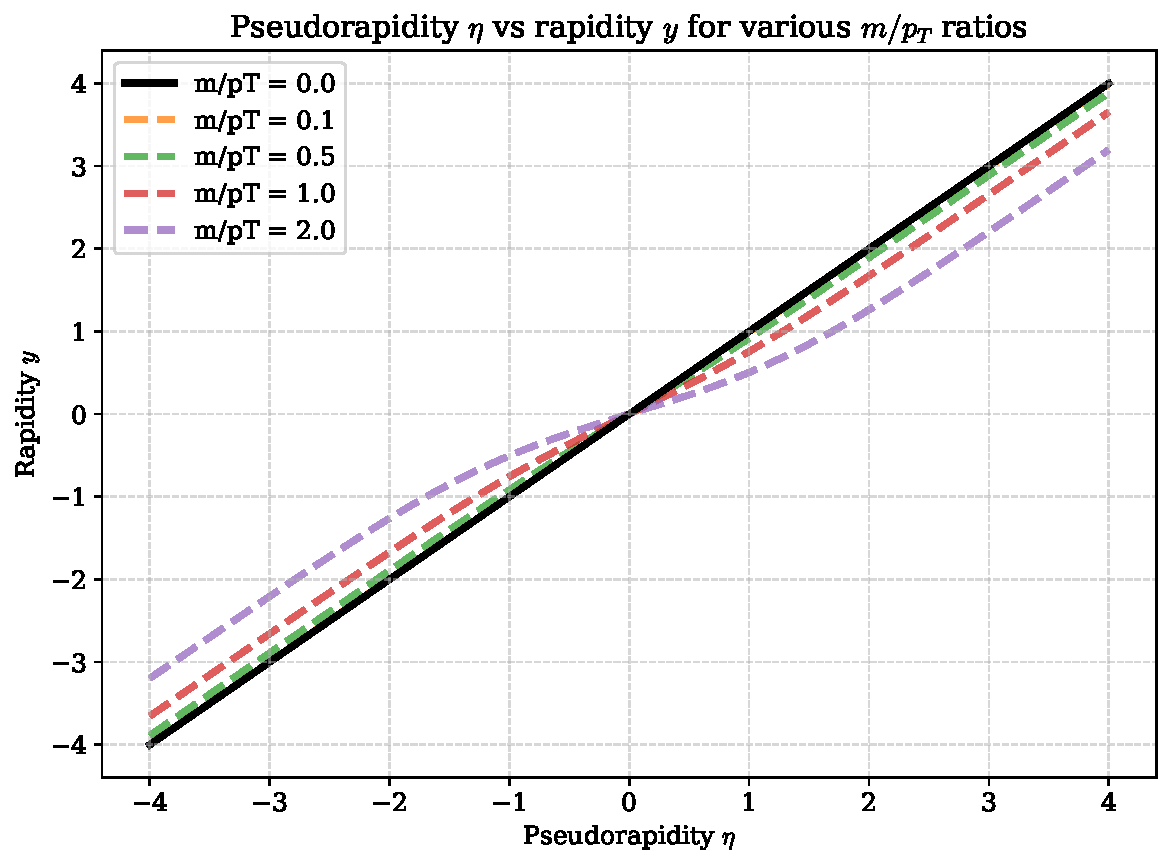
\includegraphics[width=\textwidth]{figures/chapter-01/rapidity.pdf}
  \caption[\(\eta\) vs. \(y\) for various $\nicefrac{m}{p_T}$]{%
    Comparison of pseudorapidity $\eta$ and true rapidity
    $y=\frac12\ln\frac{E+p_z}{E-p_z}$ for several mass to transverse momentum ratios.
    %
    Curves correspond to $\nicefrac{m}{p_T} = 0.0,\;0.1,\;0.5,\;1.0,\;2.0$, illustrating how finite mass distorts away from the massless limit $y=\eta$ at large $|\eta|$.
  }
  \label{fig:eta_vs_y}
\end{figure}
For massless particles, differences in \(\eta\) remain invariant under longitudinal boosts, motivating the definition of the angular distance as follows.

\begin{definition}
    The \emph{angular distance metric} is defined as
    \[
        \Delta R^2 = \Delta\eta^2 + \Delta\varphi^2,
    \]
    where \(\varphi\) is the azimuthal angle around the beam axis.
    %
    This metric approximates the geometric angle between particles in the detector while remaining approximately boost invariant.
\end{definition}
    \subsection{Statistical frameworks and uncertainty quantification.}
        In modern particle physics analyses, every measurement emerges from millions of interaction events, each carrying both statistical and systematic uncertainties.
        %
        \begin{definition}
            The \emph{Poisson distribution} is the fundamental distribution governing counting experiments.
            %
            For \(n\) observed events with expected value \(\lambda\),
            \[
                \P(n\mid\lambda) = \frac{\lambda^n e^{-\lambda}}{n!}
            \]
        \end{definition}

    In the high statistics limit, (\(n \to\infty\)), the Poisson distribution approaches a Gaussian.
    
    \begin{definition}
        The \emph{profile likelihood ratio}
            \[
                \mathcal L(\mu) = \frac{L(\mu, \hat\theta_\mu)}{ L(\hat\mu, \hat\theta)}
            \]
            where \(\hat\theta_\mu\) maximises \(L\) for fixed signal strength \(\mu\) is the optimal test statistics for hypothesis testing under the Neyman--Pearson lemma.

    \subsection{Machine learning architectures and notation.}
        Neural networks can be specified by their architecture vectors, \( [d_0, d_1,\dots, d_\ell]\), which denotes a network with input dimension \(d_0\), hidden layers of dimensions \(d_1\) through \(d_{\ell-1},\) and output dimension \(d_\ell\).

        For a network \(f: \R^{d_0} \to\R^{d_{\ell}}\) with parameters \(\theta = \qty{W_i, b_i}\), the forward pass computes
        \begin{gather}
            h_0 = x\\
            h_i = \sigma(W_i\,h_{i-i} + b_i)\quad i = 1,\dots, \ell-1\\
            f(x;\theta) = W_\ell\,h_{\ell - 1} + b_\ell
        \end{gather}
        where \(\sigma\) denotes the activation function. The universality theorem guarantees that sufficiently wide networks can approximate any continuous function.

        Training proceeds via gradient descent on a loss function \(L(\theta)\), with the gradient computed through automatic differentiation.
        
    \subsection{Information theory and optimal observables.}
        Information theory provides a rigorous framework through the Neyman-Pearson lemma, which implies that the likelihood ratio \(\frac{L(x\mid S)}{L(x\mid B)}\) provides the most powerful test for distinguishing signal \(S\) from background \(B\) at any given significance level.

        In practice, this optimal observable can be approximated using machine learning classifiers.
        %
        A well trained classifier computes
        \[
            f(x) \approx \P(S|x) = \frac{L(x\mid S)\,\P(S)}{L(x\mid S)\,\P(S) + L(x\mid B)\, \P(B)]}
        \]
        The mutual information \(I(Y; f(X))\) between the true labels \(Y\) and classifier output \(f(X)\) quantifies the information captured
        \[
            I(Y; f(X)) = \iint p(y, f)\,\log \frac{p(y, f)}{p(y)\,p(f)} \dd y\, \dd f.
        \]
        This connects directly to the area under the ROC curve and provides a model-independent measure of classification performance.

\subsection{Datasets.}
    Meaningful distinctions in particle physics data arise from the transformation between the underlying physical processes one seeks to understand and the experimental observations one can actually record, as well as from the distinction between Monte Carlo simulation and measurement in nature.
    %
    Datasets can therefore be classified according to two principal axes that capture the essential distinctions in particle physics data.
    
    The first axis distinguishes between events that occur in nature versus those generated through Monte Carlo simulation.
    %
    The second axis separates particle level quantities interest from detector level ones.

    This classification yields four distinct dataset categories, each serving a unique role in the measurement process.
    %
    Understanding the relationships between these categories plays an important role in the development of the unfolding methods discussed in this dissertation.
    \begin{figure}
    \centering
    \resizebox{\linewidth}{!}{\begin{tikzpicture}[
  font=\sffamily,
  % Global styles
  node distance=1.2cm and 2.0cm,
  >=latex,
  box/.style={
    rectangle, rounded corners, thick, draw=black, align=center,
    minimum width=2.7cm, minimum height=1.0cm,
  },
  bigbox/.style={
    rectangle, dashed, draw=black!70, rounded corners,
    inner sep=0.4cm
  },
  arrowstyle/.style={->, thick},
  doublearrow/.style={<->, thick},
  titlebox/.style={font=\bfseries\Large},
]

\tikzset{
  computer fill/.initial=blue!20,
}

\tikzset{
  computer/.style n args={1}{%
    inner sep=0, % remove inner spacing so we have full control
    % Force a phantom so that the node gets a proper size.
    execute at begin node={\phantom{\rule{2.2cm}{1.75cm}}},
    draw=none, % don't draw the node's border
    % Everything is drawn in the path picture
    path picture={
      % Force the node's overall drawing area to include the base.
      %\path[use as bounding box] (-0.2,0) rectangle (2.2,1.75);
      % Draw the monitor rectangle.
      \draw[fill=\pgfkeysvalueof{/tikz/computer fill}] (0,0.25) rectangle (2.2,1.75);
      % Draw the two “leg” lines.
      \draw[fill=\pgfkeysvalueof{/tikz/computer fill}] (0.975,0.125) rectangle (1.225,.25);
      % Draw the base rectangle.
      \draw[fill=\pgfkeysvalueof{/tikz/computer fill}] (0.6,0) rectangle (1.6,0.125);
      % Place the text inside the monitor. (Here the monitor is 2cm wide and 1.5cm tall.)
      \node[anchor=center, align=center] at (0,1.5) {#1};
    }
  }
}

% ------------------------------------------------------------------------
% Two large dashed boxes for Particle Level (left) and Detector Level (right)
% ------------------------------------------------------------------------
\node[bigbox, label={[titlebox, xshift=0.cm, yshift=.0cm]\textcolor{black}{Datasets}}](RANBox)
      at (3.125, 1) [minimum width=10.2cm, minimum height=7.2cm] {};

\node[bigbox, 
  label={[titlebox, xshift=0cm, yshift=0cm]above:\textcolor{green!40!black}{\rmfamily\bfseries\large Particle level}},
  label={[rotate=90, left, yshift=.3cm, xshift=2.25cm]left:{\rmfamily\bfseries\large Nature\quad\quad MC}}
] (particleBox) at (1,1) [minimum width=4.2cm, minimum height=5.4cm] {};

\node[bigbox, label={[titlebox, xshift=0cm, yshift=0cm]
       \textcolor{blue!60!black}{\rmfamily\bfseries\large Detector level}}] (detectorBox)
      at (5.2,1) [minimum width=4.2cm, minimum height=5.4cm] {};
\draw[dashed] (-1, 1.3) -- (7.2, 1.3);
% ------------------------------------------------------------------------
% PARTICLE LEVEL NODES (within particleBox)
% ------------------------------------------------------------------------
% Generation (middle)
\node[computer={\textbf{Generation}\\[-1.5ex]\,}, computer fill=green!20]
    (gen) at ([xshift=2cm, yshift=-1.1cm] particleBox.north west){};

\node[align=center, opacity=0.75] (truth) [below=0.75cm of gen, inner sep=0pt, 
    label={[xshift=0.05cm,yshift=0.05cm]center:{\large{\textbf{Truth}}}}]{
    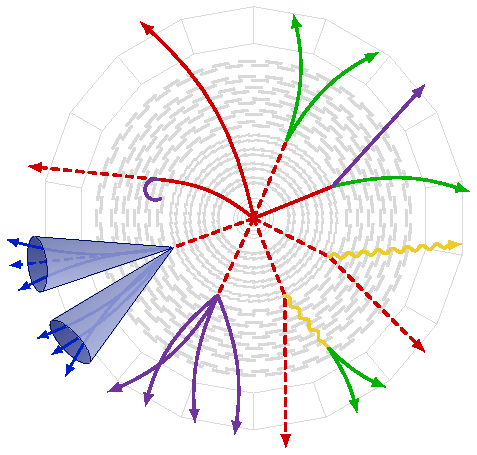
\includegraphics[width=0.2\linewidth]{figures/chapter-01/Collision.pdf}
};


% ------------------------------------------------------------------------
% DETECTOR LEVEL NODES (within detectorBox)
% ------------------------------------------------------------------------
% Data (top)
\node[computer={\textbf{Simulation}\\[-1.5ex]\;}]
  (sim) at ([xshift=2cm, yshift=-1.1cm]detectorBox.north west)
  {};

\node[align=center, opacity=0.75] (data) [below=0.65cm of sim, xshift=0cm, inner sep=0pt, 
    label={center:{\shortstack{\large\textbf{Data}}}}]{
    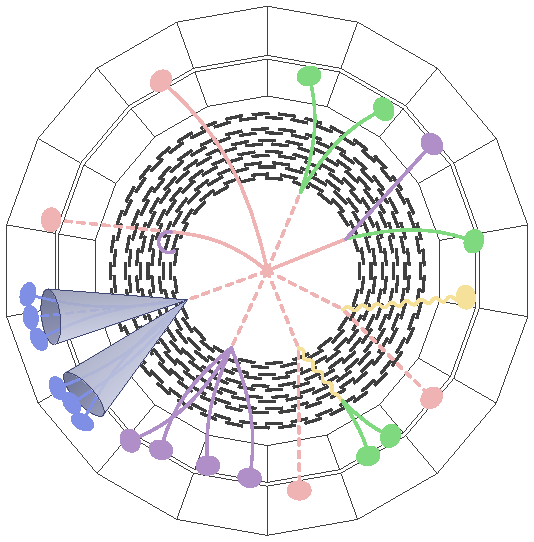
\includegraphics[width=0.2\linewidth]{figures/chapter-01/Collider.pdf}
};




% ------------------------------------------------------------------------
% Connect the re-weighted generation to re-weighted simulation
% (Emulated detector arrow)
% ------------------------------------------------------------------------
\draw[arrowstyle] (gen.east) to
  node[above, align=center, sloped, font=\footnotesize, xshift=0cm, ]{\textbf{\normalsize{Detector}}}
  node[below, align=center, font=\footnotesize, xshift=0cm]{\textbf{Simulation}}
  (sim.west);

\draw[arrowstyle] (truth.east) to
  node[above, align=center, sloped, font=\footnotesize]{\textbf{\normalsize{Detector}}}
  (data.west);

\end{tikzpicture}}
    \caption[Taxonomy of datasets used]{The four categories of data used in this dissertation organised along two orthogonal dimensions.
    %
    The vertical axis distinguishes between natural phenomena (Nature) and computational models (MC), while the horizontal axis separates particle level quantities from detector level observations.
    %
    Arrows indicate the detector response that maps particle level events to their detector level manifestations.
    }
    \label{fig:dataset-taxonomy}
    \end{figure}

\cref{fig:dataset-taxonomy} illustrates this taxonomy graphically.

    \subsubsection{Nature versus Monte Carlo.}
        The vertical dimension of \cref{fig:dataset-taxonomy} distinguishes between natural phenomena and their simulated counterparts.
        %
        Natural events represent the actual physical processes occurring in particle interactions, while Monte Carlo events are computational reproductions based on theoretical understanding.
        %
        This distinction is fundamental because although natural events contain true physics, Monte Carlo simulations provide the controlled environment necessary to understand the detector response and develop analysis techniques.

        Monte Carlo simulations incorporate theoretical knowledge, including matrix element calculations, parton shower models, and hadronisation prescriptions.
        %
        While these simulations can achieve remarkable fidelity to natural processes, they remain approximations subject to theoretical uncertainties and modelling assumptions.

    \subsubsection{Particle level versus detector level.}
        The horizontal dimension captures the transformation from particle level information to detector level signals.
        %
        Particle level quantities represent the properties of particles immediately after the hard scattering process and subsequent decay chains, before interaction with detector.
        %
        These quantities form the natural language of theoretical predictions and are directly calculable from field theory.

        Detector level quantities, in contrast, represent the actual experimental observables after particles have traversed the detector apparatus.
        %
        This transformation incorporates numerous physical effects.
        %
        The detector acts as a complex transfer function that irreversibly transforms the particle level distributions into the measured quantities.

    \subsubsection{Four dataset categories.}
        The intersection of these two dimensions yields four fundamental dataset categories.
        \begin{description}
            \item[Truth]  represents nature at the particle level---the actual physical distributions HEP experiments ultimately seek to measure.
            %
            These distributions are never directly observable but represent the ground truth that all analyses attempt to approach.
            %
            In practice, truth distributions are estimated through unfolding procedures from the information contained in the other three distributions.
            \item [Data] comprises natural events after detector effects.
            %
            It is the raw experimental output of all measurements.
            %
            Data embodies the convolution of the physics of interest with instrumental effects, making it the starting point for any experimental analysis.
            %
            The challenge lies in disentangling the physics content from the detector effects.
            \item [Generation] comprises Monte Carlo events at the particle level, providing a controlled means to understanding theoretical predictions.
            %
            Generation allows the study of particle level distributions with perfect knowledge and unlimited statistics, subject to theoretical modelling uncertainties.
            %
            Generated events serve as proxies for truth in developing and validating analysis methods.
            \item [Simulation] represents Monte Carlo events processed through detailed detector modelling, creating artificial detector level datasets with known particle level origins.
            %
            Simulation enables the study the detector response function by providing matched pairs of particle level and detector level quantities.
            %
            The fidelity of detector simulation directly impacts the ability to correct for instrumental effects.
        \end{description}
    \subsubsection{The detector response.}
        The arrows in \cref{fig:dataset-taxonomy} represent the action of the detector response function, mapping particle level distributions to their detector level counterparts.
        %
        This mapping is inherently stochastic, incorporating both resolution effects that blur distributions and acceptance effects that create blind regions in phase space.

        For natural events, this transfer function represents the actual physical processes of particle interaction with detector material---ionisation in tracking chambers, showering in calorimeters, and signal processing in readout electronics.
        %
        For simulated events, the detector simulation models these processes through programs like \textsc{Geant4} that track particles through detailed detector geometries, applying the current best understanding of particle matter interactions.

    \subsubsection{Operational framework.}
        In practice, these four dataset categories work in concert to enable precision measurements.
        %
        Paired Generation--Simulation samples provide the response matrix linking particle and detector levels, while control regions in Data validate the simulation fidelity.
        %
        Closure tests using independent Monte Carlo samples verify the unfolding procedure, and the final measurement applies these validated corrections to data to infer the underlying Truth.

        This framework implicitly assumes that the detector response is sufficiently similar between data and simulation, an assumption that must be continuously validated through auxiliary measurements and control samples.
        %
        The robustness of any measurement depends on understanding the limitations of this assumption and properly propagating the associated systematic uncertainties.

        The subsequent chapters of this dissertation will repeatedly reference these four dataset categories in the development of sophisticated methods for extracting particle level information from detector level observations.
        %
        This terminology provides the consistent language necessary for discussing the various approaches to the unfolding problem and their relative merits in different physics contexts.      
    \subsection{A note on conventions and clarity.}
         This work strives to maintain a balance between mathematical rigour and physical insight.
         %
         Where conventions differ between communities,\footnote{For example, particle physicists and machine learning researchers.} attempts are made to note both conventions.
         
\section{The Standard Model: Theoretical framework.}
The Standard Model of particle physics represents one of the most significant intellectual achievements in modern science.
%
Developed throughout the latter half of the $20^{\text{th}}$ century, it provides a quantum field theory framework that describes three of the four known fundamental forces—the electromagnetic, weak, and strong interactions---in addition to classifying all known elementary particles.
%
The mathematical formulation of the Standard Model is based on gauge theory, specifically quantum chromodynamics (QCD) and the electroweak theory, underpinned by the gauge symmetry group \(SU(3)_C\times SU(2)_L\times U(1)_Y\).

The predictive power of the Standard Model has been repeatedly validated through precision experiments across multiple energy scales, from low energy nuclear phenomena to the highest energy particle collisions achievable at modern accelerators.
%
Its crowning achievement came with the discovery of the Higgs boson in 2012 at the Large Hadron Collider (LHC)~\cite{ATLAS:2012yve, collaboration_observation_2012}, confirming the mechanism through which elementary particles acquire mass.
%
A schematic illustration of the standard model can be found in \cref{fig:sm}.

\begin{figure}
    \centering
    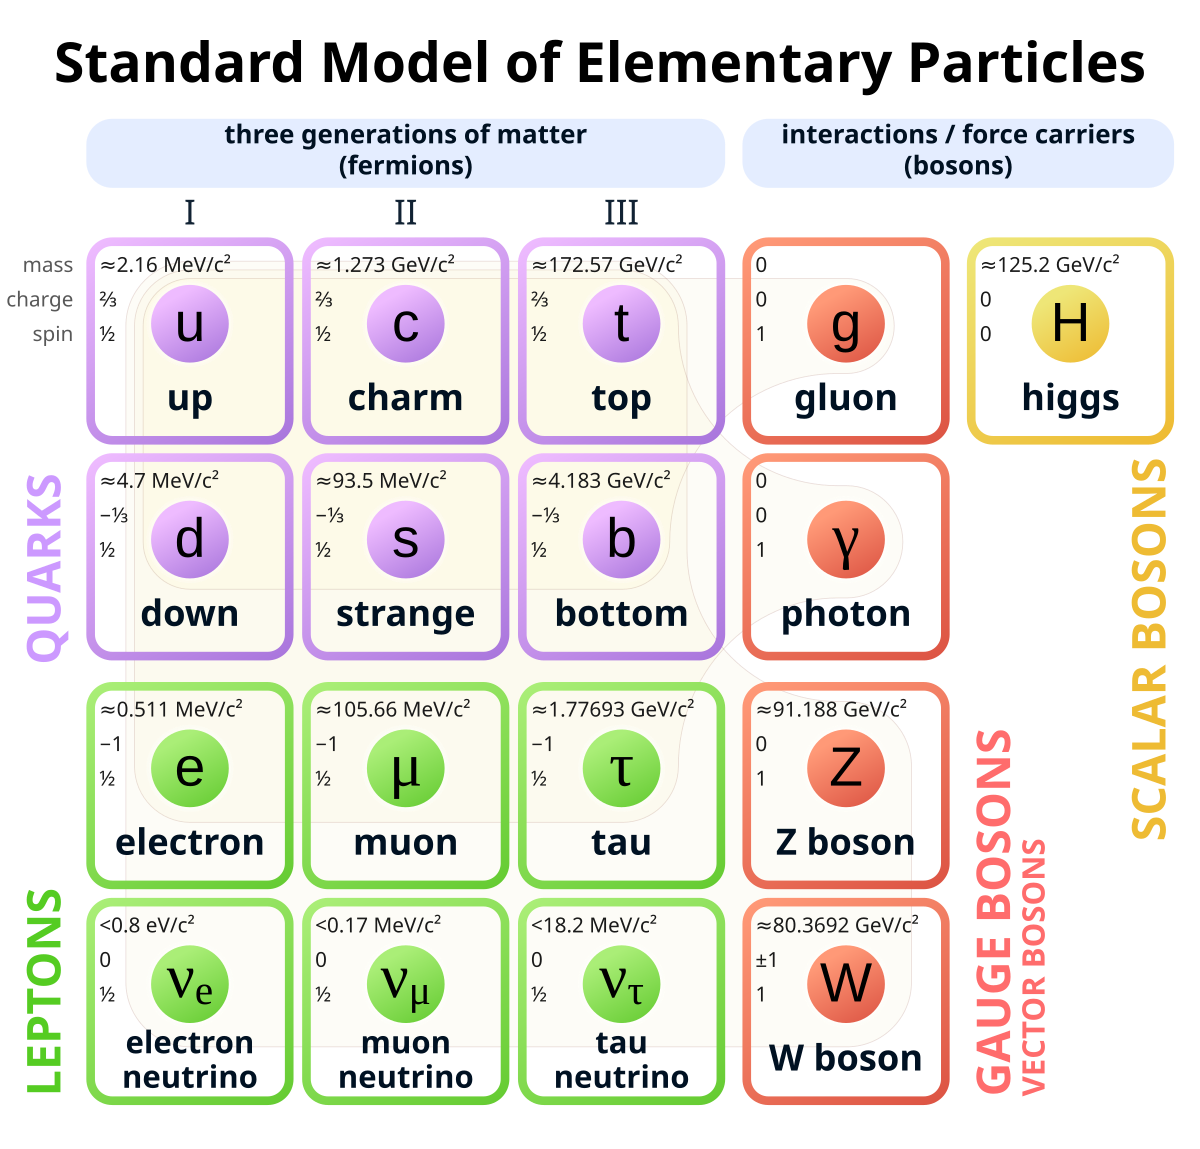
\includegraphics[width=0.75\linewidth]{figures/chapter-01/Standard_Model_of_Elementary_Particles.svg.png}
    \caption{
        A schematic illustration of the Standard Model~\cite{wiki:stdmodel}.
    }
    \label{fig:sm}
\end{figure}
\subsection{Fundamental particles and forces.}
The Standard Model categorises elementary particles into two main families: fermions, which comprise matter, and bosons, which mediate forces between matter particles.
\subsubsection{Fermions: The building blocks of matter.}
Fermions, characterized by half--integer spin, obey the Pauli exclusion principle and satisfy Fermi--Dirac statistics.
%
Fermions are further classified into quarks and leptons, each arranged in three generations of increasing mass.
\paragraph{Quarks.}
Quarks are spin $ = \nicefrac{1}{2}$ particles that are catagorised into three generations as follows:
\begin{itemize}
    \item Up (u) and down (d),
    \item Charm (c) and strange (s),
    \item Top (t) and bottom (b).
\end{itemize}

Quarks carry fractional electric charge and colour charge, and experience all fundamental forces.
%
They are confined within hadrons---composite particles categorized as baryons\footnote{three quark states, like protons and neutrons.} or mesons\footnote{quark--antiquark pairs.}.

\paragraph{Leptons.}
Like quarks, leptons too are spin \(\nicefrac12\) particles that are catagorised into three generations.
\begin{itemize}
    \item Electron (e) and electron neutrino ($\nu_e$),
    \item Muon $(\mu)$ and muon neutrino ($\nu_\mu$),
    \item Tau ($\tau$) and tau neutrino ($\nu_\tau$).
\end{itemize}

Electrons, muons, and taus carry unit electric charge and interact through the electromagnetic and weak forces, while neutrinos are electrically neutral and interact only through the weak force, making them notoriously difficult to detect.

\subsubsection{Bosons: Force carriers.}
Bosons, with integer spin values, mediate the fundamental interactions.
%
They are not subject to the Pauli exclusion principle and instead satisfy Bose--Einstein statistics.
%
The Standard Model comprises the following bosons:
\begin{description}
    \item [The photon $(\gamma)$] is a massless spin--1 boson that mediates the electromagnetic force.
    \item [$W^\pm$ and $Z$ bosons] are massive spin--1 bosons that mediate the weak force.
    \item [Gluons $(g)$] are a set of eight massless spin--1 bosons that mediate the strong force.
    \item [The Higgs boson ($H$)] is a massive spin--0 boson associated with the Higgs field that gives mass to elementary particles.
\end{description}

\subsection{Theoretical framework and symmetries.}
The Standard Model is constructed through principles of quantum field theory where particles are excitations of underlying quantum fields.
%
Its mathematical structure is determined by local gauge invariance under the following specific symmetry transformations:
\begin{description}
    \item [$\vb*{U(1)_Y}$] is associated with electroweak hypercharge and is the symmetry of electroweak theory,
    \item [$\vb*{SU(2)_L}$] describes the weak isospin, and acts on left-handed fermions, and
    \item [$\vb*{SU(3)_C}$] governs the strong interactions through colour charge in QCD.
\end{description}

Electroweak unification, demonstrated by Glashow~\cite{Glashow:1961tr}, Weinberg~\cite{Weinberg:1979pi}, and Salam~\cite{Salam:1980jd}, demonstrates how the electromagnetic and weak forces emerge as different aspects of a single electroweak interaction, which undergoes spontaneous symmetry breaking at low energies.

\subsection{The Higgs mechanism and mass generation.}
The Higgs mechanism, proposed by Peter Higgs in the 1960s~\cite{PhysRevLett.13.508}, addresses the theoretical inconsistency of massive gauge bosons in a gauge invariant theory.
%
The mechanism introduces a scalar field---the Higgs field---that permeates space and spontaneously broke the electroweak symmetry when the universe cooled after the Big Bang.

This symmetry breaking generates masses for the W and Z bosons while leaving the photon massless, explaining the significant difference between the electromagnetic and weak forces at ordinary energies. Additionally, the Higgs field couples to fermions through Yukawa interactions~\cite{DHoker1984DecouplingTheory}, generating their masses with coupling strengths proportional to the particle masses.

The discovery of the Higgs boson at the LHC in 2012, with properties consistent with Standard Model predictions, provided crucial experimental validation of this mechanism and completed the Standard Model's particle roster.

\subsection{Limitations and beyond the Standard Model (BSM) physics.}
Despite its remarkable success, the Standard Model has several well recognised limitations, including,

    \begin{enumerate}
        \item It does not incorporate gravity, the fourth fundamental force.
        \item It fails to explain the observed matter--antimatter asymmetry in the universe.
        \item It does not account for dark matter or dark energy, which together constitute about 95\% of the universe's energy content.
        \item  It requires fine tuning of parameters, raising theoretical concerns like the hierarchy problem.
        \item  It does not explain neutrino masses, which must exist given observed neutrino oscillations.
    \end{enumerate}
These limitations motivate theoretical extensions and experimental searches for physics beyond the Standard Model, including supersymmetry, grand unified theories, and various dark matter candidates.
%
Precision measurements at particle physics experiments provide one of the most powerful approaches to probe these potential extensions, making analysis techniques like those discussed in this thesis essential for advancing our fundamental understanding of nature.

\section{Fundamental role of cross section measurements in particle physics.}

Differential cross section measurements are the fundamental currency of scientific exchange in particle physics, serving as the primary bridge between theoretical predictions and experimental observations.
%
These measurements quantify the probability density of specific particle interactions as a function of kinematic variables, providing the essential link between theoretical predictions and experimental observations.
%
 A cross section quantifies the probability of a specific particle interaction occurring and is typically expressed in units of area (barns).\footnote{1 barn = \siqty{e-24}{\square\cm}.} This seemingly simple concept forms the cornerstone of how we test and validate our understanding of fundamental physics.
 
The Standard Model makes precise predictions for cross sections that can be directly tested at particle physics experiments.
%
Any statistically significant deviation between measured cross sections and theoretical predictions may signal the presence of new physics beyond the Standard Model~\cite{particle_data_group_review_2022}.\footnote{Such deviations might also signal errors in the theoretical framework used for predictions or in the experimental procedures used to measure the cross section.
} 

Cross sections are particularly powerful because they encode the underlying quantum field theory structure in a form that can be directly probed by experiment.
%
For instance, measurements of jet production cross sections at different energy scales reveal the running of the strong coupling constant \(\alpha_S\)~\cite{chiefa_parton_2025}, while precision electroweak cross section measurements constrain the properties of the Higgs boson and other fundamental particles~\cite{noauthor_precision_2006}.
%
In searches for physics beyond the Standard Model, differential cross section measurements can reveal subtle deviations that point to new particles or interactions, even when direct observation is beyond experimental reach.

These measurements also serve a crucial role in constraining effective field theories (EFTs) that parameterise potential new physics in a model independent way.
%
By measuring differential distributions with high precision, experiments can place bounds on EFT coefficients, narrowing the space of viable theoretical extensions to the Standard Model~\cite{contino_validity_2016}.

For example, the ongoing precision program at the Large Hadron Collider (LHC) relies heavily on refined cross section measurements to extract maximum physical insight from collected data.
%
In addition to driving comparisons with theoretical models, cross section measurements are also used at high energy physics experiments for MC tuning~\cite{albert_antares_2025} and consistency checks~\cite{buckley_constraints_2025} among other applications.

\section{Cross section measurements: From theory to experiment.}
\subsection{Theory.}
    Classically, the cross section (\(\sigma\)) represents the effective area within which two particles must interact for a particular process to occur.
    %
    \begin{definition}
        For collisions between discrete particles, the \emph{cross section} is defined as the area transverse to their relative motion.
        %
        If the particles were to interact via contact forces (e.g., hard spheres), the cross section corresponds to their geometric size.
        %
        For long range forces however, the cross section is larger than the physical dimensions of the particles due to action--at--a--distance effects.
    \end{definition}
%

    \begin{definition}
        The \emph{differential cross section} (\(\frac{d\sigma}{d\Omega}\)) provides additional granularity by describing how the probability of scattering depends on specific final state variables, such as scattering angle (\(\theta\)) or energy transfer.
        %
        It is defined as
        \begin{equation}
            \frac{\dd\sigma}{\dd\Omega} = \frac{\text{Number of events scattered into } \dd\Omega}{\text{Incident flux} \times \text{Target density}}.
        \end{equation}
    \end{definition}

    The total cross section can be recovered by integrating over solid angle:
    \begin{equation}
    \sigma = \int_{4\pi} \frac{\dd\sigma}{\dd\Omega} \, \dd\Omega.
    \end{equation}

    While the classical picture above is intuitive, scattering at HEP experiments is governed by quantum field theory (QFT).
    %
    In this framework the probability for a process is encoded in a Lorentz invariant matrix element \(\mathcal{M}\).
    
    For a \(2 \to n\) reaction with incoming \(4-\)momenta \(p_{1,2}\) and final state phase space \( \dd\Phi_n \), the fully differential cross section is

    \begin{equation}
      \dd\sigma =
      \frac{(2\pi)^4 \, \delta^{(4)}\!\bigl(p_1 + p_2 - \sum_{i=1}^n p_i\bigr)}
           {4\,\sqrt{(p_1\!\cdot\!p_2)^2 - m_1^2 m_2^2}}
      \; |\mathcal{M}|^2 \;
      \dd\Phi_n,
      \label{eq:qft_xsec}
    \end{equation}
    where the denominator is the flux factor and \(\dd\Phi_n = \prod_{i=1}^{n} \tfrac{\dd^3 p_i}{(2\pi)^3 2E_i}\) is the Lorentz invariant phase space element.\footnote{Standard derivations can be found in \cite{peskin_introduction_1995,Navas2024ReviewPhysics, Hollik2014Quantum978-1-107-03473-0, QuantumAssessment}.
    }
    %
    \cref{eq:qft_xsec} reduces to the classical area when \(|\mathcal{M}|^2\) is replaced by a contact interaction and the final state integral collapses to a single kinematic configuration.
    %
    Integrating \cref{eq:qft_xsec} over final state kinematics yields the total cross section, \(\sigma = \int \dd\sigma\).
    
    At tree level, \(|\mathcal{M}|^2\) is computed from Feynman rules derived from the Lagrangian, while higher order corrections incorporate loops, parton showers, and non-perturbative effects such as hadronisation.
    %
    For practical experimental predictions predictions one folds \(|\mathcal{M}|^2\) with parton distribution functions (PDFs) and convolves the result with detector response---precisely the forward process that the unfolding methods developed in this thesis seek to invert.

Differential cross sections have a long history of providing valuable insights for probing fundamental properties of particles and interactions.
%
Their use dates all the way back to Rutherford's scattering experiments that revealed the existence of atomic nuclei by analysing angular distributions of scattered alpha particles \cite{F.R.S.1911LXXIX.Atom}.

    \subsection{Experimental Measurement}
    \label{subsec:exp_measurement}
        At modern colliders\footnote{
            This section focusses on collider experiments, but similar analyses can be applied to non-collider HEP experiments as well, such as fixed target experiments.
            %
            \cite{leo_techniques_1994} and chapters \numrange{31}{38} of \cite{particle_data_group_review_2022} provide a comprehensive and detailed exposition of experimental measurement in HEP.
            %
            \cite{Brodsky2013PhysicsBeams, AveryCrossRates} focus specifically on fixed target techniques and phenomenology.
            %
            \cite{MuheimNuclearLaws} compares collider and fixed target formalisms, reviews luminosity analogues, and details the role of detector simulations and unfolding in a fixed target context
        } the two beams themselves act as both ``projectile'' and ``target.'' 
        %
        The basic experimental quantity is the instantaneous luminosity.
        \begin{definition}
            The \emph{luminosity} \(\mathcal{L}(t)\) is defined such that the interaction rate for a process with cross section \(\sigma\) is \(\dd N/\dd t = \mathcal{L}(t)\,\sigma\).
        \end{definition}

        Time integrating over a data taking period \([t_0, t_f]\) yields the integrated luminosity.
        \begin{definition}
            The \emph{integrated luminosity} \(\mathcal{L}_{\text{int}}\) is defined as
            \begin{equation}
                \mathcal{L}_{\text{int}}
                = \int_{t_0}^{t_f} \mathcal{L}(t)\,\dd t,
                \qquad
                \sigma
                = \frac{N_{\text{obs}} - N_{\text{bkg}}}
                       {\mathcal{L}_{\text{int}}\,\epsilon\,A}.
                \label{eq:crossec_collider}
              \end{equation}
              Here \(N_{\text{obs}}\) is the number of selected events, \(N_{\text{bkg}}\) an estimate of background contaminations, \(\epsilon\) the detector and selection efficiency and \(A\) the geometric--plus--kinematic acceptance of the analysis.
        \end{definition}


        For binned measurements one bins events in an observable \(X\)\footnote{For example, transverse momentum \(p_T\) or rapidity \(y\)} and divides by the bin width.
        \begin{equation}
          \frac{\dd\sigma}{\dd X}\Big|_{X_i}
          = \frac{1}{\mathcal{L}_{\text{int}}\,\Delta X_i}
            \frac{N_i^{\text{obs}} - N_i^{\text{bkg}}}
                 {\epsilon_i\,A_i},
          \label{eq:diff_crossec_collider}
        \end{equation}
        with the index \(i\) denoting the \(i^{\text{th}}\) bin.

        Luminosity determination is itself a precision measurement, usually performed with dedicated luminometers that exploit van der Meer scans or pileup counting techniques.
        %
        The efficiency--acceptance term \(\epsilon\,A\) is obtained from full detector simulations and corrected in data using control samples and ``tag--and--probe'' methods.

        \cref{eq:crossec_collider,eq:diff_crossec_collider} thus link the theoretically calculated parton level cross sections (\textit{vide}\cref{eq:qft_xsec}) to the raw observables recorded by the a detector, completing the chain from theory to experiment.

    \subsection{Applications in particle physics.}
        As mentioned above, cross section measurements serve as the fundamental currency of particle physics, translating abstract theoretical predictions into measurable experimental quantities.
        %
        However, their applications extend far beyond simple theory validation into the operational heart of how experiments function, analyse data, and cross--validate results.
        \subsubsection{Theory validation.}
            As discussed above, comparing measured cross sections with predictions from quantum field theory validates and tests theoretical models like quantum chromodynamics and electroweak theory, by encapsulating interaction probabilities in a measurable form.
            %
            Deviations from expected cross sections may indicate new phenomena, such as supersymmetric particles or dark matter candidates.
            
            Differential cross sections also provide constraints on effective field theories and parton distribution functions (PDFs), essential for understanding the internal structure of hadrons.
            %
            Unfolded cross section measurements allow comparisons with theoretical models years after data collection, even if detector simulations are no longer available, further enhancing their utility, and future proofing the data.
            %
            Their determination requires careful design and analysis techniques to account for systematic uncertainties introduced by detector effects.

        \subsubsection{Monte Carlo tuning.}
            \begin{definition}
                \emph{Monte Carlo tuning} is the iterative process of adjusting simulation parameters to match measured cross sections, ensuring that detector simulations accurately reproduce real experimental data.
            \end{definition}
            %
            Cross section measurements are extensively used in Monte Carlo (MC) tuning.
            
            Every particle physics analysis relies on sophisticated simulations that model everything from the initial parton interactions through hadronisation to the detector response.
            %
            These simulations contain dozens of phenomenological parameters, such as the strong coupling constant at various scales and non-perturbative fragmentation functions.
            \begin{definition}
                \emph{Parton distribution functions} (PDFs) are probability distributions that describe the probability of finding a parton (quark or gluon) in a hadron at a given momentum fraction \(x\) and scale \(Q^2\).
                %
                PDFs are determined from global fits to a wide range of hard scattering processes, including deep inelastic scattering, Drell--Yan production, and jet production.
            \end{definition}
            %
            Measured cross sections provide the ground truth that anchors these simulations to reality.

            Consider the following example:
            %
            When CMS measures the inclusive jet cross section at a new centre--of--mass energy, that measurement immediately becomes a crucial input for tuning generators like \textsc{Pythia} or \textsc{Herwig}.
            %
            The differential distributions---whether in transverse momentum, rapidity, or invariant mass---reveal where the models succeed and where they fail.
            %
            A discrepancy in the high\(-p_T\) tail might indicate a need to adjust the modelling of initialstate radiation; unexpected structure in angular distributions could point to missing higher order QCD effects.
        \subsubsection{Consistency checks.}
            Cross--validations between different experimental approaches, detector configurations, or analysis methods ensure measurement reliability and identify systematic biases.
            %
            Cross sections serve as essential tools for consistency checks across multiple dimensions of experimental physics.
            %
            Within a single experiment, measuring the same process through different decay channels provides a powerful systematic cross check.
            %
            For instance, measuring the W boson production cross section through both electronic and muonic decays tests the understanding of lepton universality while simultaneously validating detector calibrations.
            %
            Any significant deviation signals either new physics, errors in the phenomenological method used, or unaccounted systematic effects.
            
            Between experiments, cross section measurements enable crucial cross--experiment validation.
            %
            When CMS and ATLAS measure the same process with independent detectors and analysis chains, agreement within uncertainties validates both measurements.
            %
            Disagreement, conversely, can reveal subtle systematic effects or push calculations to higher precision.

            These applications cascade through every level of experimental operations.
            %
        \subsubsection{Luminosity determination.}
            Luminosity determination becomes possible through processes with well--known theoretical cross sections.
            %
            Van der Meer scans calibrate the absolute luminosity scale, but elastic scattering and other standard candle processes provide continuous monitoring.
            %
            The uncertainty on integrated luminosity, typically \numrange{2}{3}\%, directly impacts every cross section measurement, creating a web of interdependencies.
            
        \subsubsection{Background estimation.}
            Background estimation in searches for new physics relies on measured cross sections of Standard Model processes.
            %
            When searching for supersymmetric particles, the irreducible backgrounds from \(W\, +\) jets or \(t\bar t\) production must be understood at the percent level.
            %
            Control regions enriched in backgrounds, combined with precise cross section measurements, enable data driven background estimates that would be impossible from simulation alone.
        \subsubsection{Parton luminosity.}
            \begin{definition}
                \emph{Parton luminosity} is the effective luminosity for specific parton--parton interactions, calculated by convolving the total luminosity with parton distribution functions.
            \end{definition}
            %
            A particularly elegant application of cross sections emerges in parton luminosity calculations.
            %
            Since protons are composite objects, the effective luminosity for producing heavy particles depends on the convolution of PDFs with the partonic cross section.
            %
            Measurements of Drell--Yan production at different invariant masses directly probe the quark and antiquark distributions, while inclusive jet production constrains the gluon PDF.
            %
            This creates a self--consistent feedback loop, where better PDFs enable more precise predictions, which enable more sensitive measurements, which further constrain the PDFs.
            
        \subsubsection{Detector performance validation.}
             Detector performance validation represents another major application of cross section measurements.
             %
             Measured cross sections for well understood processes serve as standard candles for monitoring detector stability over time.
             %
             For example, slow drift in the measured \(Z\to\mu\mu\) cross section might indicate degrading muon chamber performance long before it would be noticed in individual event displays.
             %
             These measurements become part of the experiment's data quality monitoring, flagging problems in real time.
            \subsubsection{Systematic uncertainty evaluation.}
                The role of cross section measurements in systematic uncertainty evaluation cannot be overstated.
                %
                Every measurement must account for theoretical uncertainties in signal and background processes.
                %
                By measuring auxiliary cross sections, for instance, \(Z\, +\) jets production when studying \(W\, +\) jets, experiments can constrain these uncertainties using data rather than relying solely on theoretical estimates.
                %
                This \textit{in situ} constraint often reduces systematic uncertainties by factors of two or more.
            \subsubsection{Future planning.}
                Finally, cross sections enable physics program planning for future experiments.
                %
                The measured production rates at current energies, extrapolated using theoretical calculations, determine required luminosities and detector capabilities for next--generation experiments.
                %
                For exmaple, the surprisingly large Higgs production cross section at the LHC, for instance, has already influenced design considerations for future electron--positron Higgs factories.
    \vskip{1em}            
    In sum, cross sections certainly do function as the Rosetta Stone of particle physics, translating between the languages of theory, simulation, and experimental measurement while maintaining coherence across all three domains.
    %
    However, they serve not merely as endpoints of analyses, but as the connective tissue that binds together theory, simulation, and experiment into a coherent whole.
    %
    They simultaneously test theoretical understanding, calibrate experimental tools, and point the way toward new discoveries.
    %
    This multiplicative utility explains why cross section measurements, even of well studied processes, remain at the heart of every particle physics experiment.

\section{Detector response in precision measurements.}
    The direct comparison between theoretical predictions and experimental measurements is complicated by detector effects.
    %
    HEP detectors are technological marvels that capture the trajectories of charged particles, energy deposits in calorimeters, and timing and pattern--recognition information from tracking and particle--identification systems, but they introduce distortions that must be carefully accounted for to extract the true physical distributions of interest.
    %
    Particle physics detectors represent some of humanity's most sophisticated sensing apparat\=us—--capturing particle trajectories with silicon sensors operating at liquid helium temperatures, measuring energy deposits in dense calorimeter crystals, and reconstructing vertices with sub--millimetre precision.
    %
    Yet these technological marvels inevitably introduce systematic distortions that transform the pristine theoretical predictions into the messy reality of experimental data.
    
    Consider the information degradation that occurs in every measurement. 
    %
    Finite resolution creates fundamental blurring, much like how a camera lens distorts an image.
    %
    The detector's discrete sensing elements can only measure particle energies, momenta, and positions to finite precision, creating an inherent convolution between the true physics distribution and the instrument response function.
    %
    Geometric acceptance imposes hard boundaries on observable phase space.
    %
    Particles scattered into the forward beam pipe or extreme backward angles simply vanish from the recorded dataset, creating holes in the measurement that no amount of statistics can fill.
    
    Detection efficiency varies across the detector's active volume, introducing a complex weighting function that depends on particle type, energy, and trajectory.
    %
    A high--energy muon might traverse the entire detector with near--perfect efficiency, while a low--energy hadron could be absorbed in the first layers of material.
    %
    Particle misidentification compounds these challenges through cross--contamination between categories, such as when hadronic shower fluctuations cause a pion to masquerade as a kaon~\cite{belle_collaboration_precision_2013}.

    In this way every detector measurement embeds two irreducible probability relationships.
    \begin{description}
        \item [Detection incompleteness] \(\P(\text{measured}\mid\text{true}) < 1\) True events that fail to be recorded
        \item [Measurement impurity] \(\P(\text{true}\mid\text{neasured}) < 1\) Recorded events that represent contamination
    \end{description}
    This demonstrates why detector corrections are fundamentally different from simple calibrations.
    %
    Unlike adjusting a scale that consistently reads, say, \(5\%\) high, detector response involves dual information loss that operates asymmetrically.
    
    The first inequality captures the selection bias where certain true configurations have zero probability of detection, creating null spaces in the measurement.
    %
    The second inequality captures the contamination bias where every reconstruction category contains some fraction of misclassified events.
    
    Background contamination represents a third problem---every measurement category contains some admixture of misclassified events.
    %
    When hadrons interact in electromagnetic calorimeters, they can mimic electron signatures.
    %
    When cosmic ray muons traverse the detector during a collision, they contribute to the muon count despite having no connection to the physics of interest.
    %
    This contamination creates what in signal processing is called the false positive rate.
    
    The mathematical relationship between true particle level distributions and observed detector level measurements follows the convolution integral
    \[
        \label{eq:forward-folding}
        p(x) = \int r(x\mid z)\;p(z)\; \dd z
    \]
    Where \(p(x)\) is the detector level density, \(p(z)\) is the particle level density and \(r(x\mid z)\) serves as the response kernel, the conditional probability density that maps each possible true configuration \(z\) to the distribution of possible detector measurements \(x\).
    %
    This kernel encapsulates the entire cascade of finite resolution information degradation.
    
    The response kernel is analogous to the optical transfer function in image processing.
    %
    It describes how the ``lens'' of the detector blurs and distorts the perfect theoretical ``image''.
    %
    The response function inherently embeds both probabilistic asymmetries.
    %
    Regions where \(\int r(x\mid z)\;\dd x < 1\) reveal acceptance holes, i.e. true configurations that produce no detector signal whatsoever.
    %
    Conversely, the convolution structure itself ensures that multiple truth distributions can yield identical detector observations, creating the degeneracy problem that makes direct inversion impossible.
    
    A central challenge then, for particle physics, is inverting this response kernel to recover \(p(z)\) from observed data \(p(x)\).
    %
    This inversion is mathematically ill--posed precisely because of the information loss.
    %
    Standard matrix inversion fails catastrophically, amplifying statistical noise into wild oscillations that bear no resemblance to the underlying physics.
    
    The resolution requires sophisticated regularisation methods that impose additional constraints such as smoothness assumptions, positivity requirements, and prior knowledge about the expected signal shape.
    %
    These constraints transform the ill--posed inverse problem into a well defined statistical inference challenge, though at the cost of introducing systematic uncertainties that must themselves be carefully validated.
    
    The detector response problem exemplifies a universal pattern in experimental science: the tension between instrumental precision and information preservation.
    %
    From astronomical imaging through medical diagnosis to HEP measurements, the fundamental trade off between sensitivity and purity governs all attempts to extract signal from noise.

\section{Challenges at modern experiments.}
    Several challenges at the modern HEP experiments make cross section measurements particularly demanding.

    \begin{description}
        \item [High dimensional phase spaces] Modern measurements often involve multiple correlated observables, creating high dimensional distributions that are difficult to analyse with traditional methods.
        \item [Limited statistics in extreme regions] Rare processes or the tails of distributions often contain valuable physics information but suffer from limited statistics.
        \item [Complex detector effects] Detectors have non-trivial response functions that can vary significantly across phase space, and are only known implicitly through precision simulations. Their explicit functional form is unknown.
        \item [Theoretical uncertainties] Precision measurements are increasingly limited by theoretical uncertainties in both signal and background modelling.
        \item [Computational constraints] Detailed simulation of detector response requires substantial computing resources, limiting the statistical precision of response modelling.
    \end{description}

    These challenges make the unfolding problem increasingly difficult, particularly as measurements probe more complex final states and differential distributions.
    %
    For example, measurements of jet substructure, which probe the detailed radiation pattern within collimated sprays of particles, involve observables with complex correlations and detector effects that vary based on jet energy, rapidity, and substructure properties themselves~\cite{Larkoski2020JetLearning, kogler_jet_2019, mozer_jet_2017}.
    
    The need for unfolding arises from the fundamental requirement to present results in a detector independent form that can be directly compared with theory predictions or results from different experiments.
    %
    Without this correction, theoretical interpretations would need to incorporate experiment specific detector simulations, significantly complicating scientific exchange and theoretical analysis, and inter--experiment comparisons would simply not be possible.

\section{Thesis scope and physics impact.}

This dissertation focuses on developing, analysing, and applying novel machine learning methods for cross section measurements in particle physics, with particular emphasis on unbinned approaches that overcome limitations of traditional techniques. The work spans the spectrum from improving binned methods with neural posterior estimation to completely unbinned approaches for both full distributions and statistical moments.

The primary contributions of this thesis include:

\begin{enumerate}
\item Development of \textsc{Neural Posterior Unfolding} (NPU), enhancing binned approaches through normalising flows and amortised inference.
\item Introduction of \textsc{Moment Unfolding}, directly deconvolving distribution moments without binning.
\item Creation of \textsc{Reweighting Adversarial Networks} (RAN), a general framework for unbinned spectrum unfolding.
\item Analysis of event correlations in unfolded data and their impact on uncertainty estimation.
\item Investigation of symmetry discovery with \textsc{SymmetryGAN} and its connections to measurement constraints.
\end{enumerate}

These methodological advances address fundamental challenges in experimental particle physics, potentially enhancing the precision and scope of measurements at present and future HEP experiments.
%
These methods can have a wide range of applications in particle physics, including:

\begin{itemize}
\item Improved precision in jet substructure measurements, enabling better discrimination between different theoretical models of QCD radiation.
\item Enhanced sensitivity to effective field theory parameters by directly deconvolving distribution moments.
\item More robust uncertainty quantification in high dimensional measurements.
\item Computational efficiency gains allowing for more detailed systematic studies.
\item A rigorous statistical framework for incorporating detector response uncertainties in the unfolding process.
\end{itemize}

By bridging sophisticated machine learning techniques with the specific requirements of particle physics measurements, this work aims to advance the ability to extract fundamental physical insights from complex experimental data.
%
The methods developed here have applications beyond particle physics, potentially benefiting any field where deconvolution of instrumental effects is necessary for scientific inference.
\chapter{Theoretical Foundations}
\label{chap:theoretical-foundations}
\section{Statistical Formulation of the Unfolding Problem}

Unfolding, also known as deconvolution, is the process of correcting detector distortions in experimental data to recover the true particle--level distributions.
%
This procedure is critical for comparing experimental results with theoretical predictions and for enabling detector--independent analyses.
%
The unfolding problem is inherently statistical and presents unique challenges due to its ill-posed nature.

\subsection{The Detector Response and Forward Problem}

The relationship between the particle--level truth distribution \(p(z)\) and the detector--level measured distribution \(p(x)\) is governed by the detector response function \(r(x|z)\), which encapsulates the resolution effects.\footnote{Efficiency and acceptance effects can also be incorporated if ``empty" events are allowed.}
\begin{equation}
    p(x) = \int r(x|z)\; p(z) \, \dd z.
\end{equation}
This equation describes the \textbf{forward problem}, where the true distribution \(p(z)\) is mapped to the measured distribution \(p(x)\).
%
The detector response function \(r(x|z)\) can often be estimated through detailed simulations.

\subsection{The Inverse Problem: Unfolding}

The goal of unfolding is to invert the forward problem and estimate truth, \(p(z)\) from data \(p(x)\).
%
Mathematically, this requires solving:
\begin{equation}
    p(z) = \int r^{-1}(z|x) \;p_{\text{measured}}(x) \, \dd x,
\end{equation}
where \(r^{-1}(z|x)\) represents the inverse response kernel.
%
However, this inversion is ill--posed because small fluctuations in \(p(x)\) can lead to large variations in \(p(z)\).
%
Regularization techniques are therefore essential to stabilize the solution.

\subsection{Likelihood-Based Formulation}
    In practice, unfolding is performed using statistical inference methods.
    %
    Given a set of measured data \(\mathbf{X}_{i=1}^N\), the likelihood function for a proposed truth distribution \(p(z; \theta)\), parametrised by \(\theta\), is
    \begin{equation}
        \mathcal{L}(\theta; \mathbf{X}) = \prod_{i=1}^{N} p(x_i;\; \theta),
    \end{equation}
    where
    \begin{equation}
        p(x; \theta) = \int r(x|z) \;p(x; \theta) \, \dd z.
    \end{equation}
    Maximizing this likelihood yields an estimate of the parameters \(\theta\), which define the unfolded truth distribution.
    %
    Regularization can be incorporated into this framework by adding penalty terms to the likelihood or by constraining the parameter space.

    \subsection{Regularization Techniques}
        Regularization mitigates the instability of unfolding by imposing constraints on the solution.
        %
        Common approaches include Tikhonov Regularization~\cite{Karl2005RegularizationReconstruction}, in which one adds a penalty term proportional to the norm of the second derivative of \(p(z)\), enforcing smoothness, and iterative methods which gradually refine estimates of \(p(z)\), regularizing by stopping before convergence.
        %
        These techniques balance fidelity to the measured data (prior independence) with stability of the unfolded solution.

    \subsection{Challenges in High Dimensional Phase Spaces}
    \label{subsec:challenges-in-high-dimensional-phase-spaces}
        \subsubsection{Binned methods}
        \label{subsubsec:binned-methods}
            A significant challenge that traditional unfolding methods face is the \emph{curse of dimensionality}.
            %
            As the number of measured observables increases, the statistical power required to populate discrete bins grows exponentially, quickly overwhelming even the largest datasets collected at modern experiments.
    
            Consider a measurement involving just four kinematic variables: transverse momentum, pseudorapidity, azimuthal angle, and invariant mass.
            %
            With a modest 20 bins per dimension, the resulting joint histogram requires \(\num{1.6d5}\) bins. Most of these bins will contain zero events, creating a sparse matrix that renders traditional unfolding techniques numerically unstable.
            %
            The relative uncertainty can scales as
            \begin{equation}
            \label{eq:relative-uncertainty}
                \text{Relative uncertainty} \propto \frac{1}{\sqrt{N_{\text{events}}} \cdot \prod_{i=1}^d \Delta z_i},
            \end{equation}
            where \(\Delta z_i\) are bin widths.
            %
            This scaling relationship emerges directly from Poisson counting statistics applied to multi--dimensional histograms.
            %
            For any histogram bin containing \(N\) events, the statistical uncertainty follows the standard Poisson scaling \(\sigma\propto\sqrt{N}\), yielding a relative uncertainty of \(\nicefrac{1}{\sqrt{N}}\).
            %
            In a \(d-\)dimensional measurement with bin widths \(\Delta z_1, \Delta z_2, \dots, \Delta z_d\), each bin occupies a hyper-volume
            \[
                V = \prod_{i=1}^d\Delta z_i
            \]
            in the measurement space.
            %
            Assuming approximately uniform event density, the expected number of events in any given bin scales as
            \[
                N_{\text bin} \propto N_{\text events} \times \prod_{i=1}^d\Delta z_i.
            \]
            The relative uncertainty in the measured differential quantity therefore follows the scaling law in \cref{eq:relative-uncertainty}.
            %
            This relationship reveals why traditional binned methods become increasingly impractical as dimensionality increases: maintaining fixed statistical precision requires exponentially more data or exponentially coarser binning, both of which severely limit the measurement's resolving power.
            
            Beyond a point, \textit{response matrix}, \(\mathbf{R}\) becomes not just ill--conditioned but genuinely rank--deficient, as sufficiently many bins have not just few events in them, but rather no events in them at all.
            %
            Hence, entire swaths of phase space remain unmeasurable regardless of accumulated statistics.
    
            \emph{Binning artifacts} compound these statistical challenges through systematic information loss.
            %
            The process of discretising continuous distributions into finite bins introduces artificial boundaries  onto the underlying physics.
            
            This discretization becomes particularly pernicious when dealing with correlation structures that span multiple dimensions.
            %
            Real particle collisions generate complex kinematic relationships---the angular distribution of decay products correlates with their energies, jet substructure variables depend on the overall jet momentum, and detector response functions couple seemingly independent observables.
            %
            Binning destroys these correlations by requiring low dimensional projections.
            %
            For instance, in jet substructure measurements, the relationship between different substructure variables contains valuable information about the underlying physics that can be obscured by independent binning of each variable.
            %
            Moreover, many theoretical predictions in particle physics are at the level of statistical moments or other distribution properties rather than full differential spectra.
            %
            Traditional unfolding methods require first unfolding the full distribution and then calculating these properties, which can lead to reduced precision in the moment predictions.
    
            The computational burden grows even faster than the statistical requirements.
            %
            Matrix inversion algorithms scale as \(\mathcal O(N^3)\) with bin number, meaning that the aforementioned four--dimensional histogram with \(\num{1.6d5}\) bins requires approximately \(\mathcal{O}(\num{d16})\) floating point operations to invert.
            %
            More fundamentally, the \emph{null spaces} and \emph{degeneracies} that plague two dimensional unfolding become dramatically worse in higher dimensions, where multiple truth configurations can project to identical detector signatures along numerous measurement axes simultaneously, because high dimensional measurements create complex geometric relationships between true and observed phase spaces.

            In addition to these limitations, traditional binned approaches suffer from an additional systematic weakness;
            %
            the response matrix \(R\) depends on on numerous variables that are typically marginalized over in order to bin the data.
            %
            While conventional methods construct \(R\) based on a limited set of binned observables, the true detector response depends on a much richer set of event characteristics.
            %
            These include additional kinematic variables not captured in the chosen binning scheme, event level properties such as particle multiplicity and missing energy, detector conditions like instantaneous luminosity and pileup activity, and correlations with other particles produced in the same collision.
            %
            Traditional unfolding methods are effectively forced to assume that \(R\) remains constant when averaged over these marginalized variables, but this assumption is patently incorrect when the detector response varies systematically across different regions of this extended phase space.
            %
            For example, the energy resolution for jets may depend not only on the jet's transverse momentum and pseudorapidity, variables often chosen for binning, but also on the jet's substructure, the presence of nearby particles, and the overall event topology.
            %
            By marginalising over these features, binned methods introduce systematic biases that can propagate through the unfolding procedure and distort the final measurements in ways that are difficult to quantify or correct.

        \subsubsection{Unbinned methods}
        \emph{Unbinned approaches} emerge as a natural response to these challenges, operating directly on individual events rather than aggregated histogram counts.
        %
        These methods exploit the event level structure that binning destroys, preserving the full kinematic information and correlation patterns within each recorded data point.
        %
        Instead of discretizing phase space into predetermined categories, unbinned techniques allow the data itself to determine the relevant resolution scales and correlation structures.
        
        Rather than explicitly modelling the response function \(r(x|z)\), modern techniques like \textsc{OmniFold}~\cite{andreassen_omnifold_2020} employ iterative reweighting strategies that learn implicit mappings between truth and detector-level distributions.
        %
        These methods sidestep the curse of dimensionality by avoiding explicit probability density estimation, instead focusing on weight optimization that preserves marginal distributions while respecting the detector response.

        The computational complexity shifts from matrix algebra to optimization landscapes, that scale more favourably with dimensionality.
        %
        While traditional unfolding requires inverting matrices that grow exponentially with dimension, unbinned methods typically employ gradient--based optimization that scales polynomially.
        %
        This trade-off exchanges the well--understood numerical properties of linear algebra for the more complex but ultimately more scalable challenges of machine learning optimization.

        Yet this transition introduces new sensitivities to model and hyperparameter choices that traditional methods avoid.
        %
        The implicit effect of the learning dynamics make it crucial to understand how optimization biases influence the final results.
        %
        These considerations establish the foundation for exploring how modern machine learning approaches navigate these challenges while preserving the statistical rigour that particle physics demands.

\section{Forward and Inverse Problems in HEP}
    The measurement process in high-energy physics experiments inherently involves two complementary mathematical challenges: the forward problem of predicting detector responses from particle-level interactions, and the inverse problem of recovering true physics distributions from observed detector measurements. These twin challenges form the conceptual foundation for understanding detector effects and developing unfolding methodologies.

\subsection{Mathematical Formulation}

The relationship between particle--level truth distributions and detector--level observations is governed by the Fredholm integral equation of the first kind~\cite{fredholm_sur_1903}
\begin{equation}
    p(x) = \int r(x|z)\,p(z) \, \dd z + \epsilon(x),
\end{equation}
where \(p(z)\) represents the true particle--level distribution, \(r(x|z)\) is the detector response kernel encoding resolution effects and acceptance, \(p(x)\) is the observed detector-level distribution, and \(\epsilon(x)\) accounts for measurement noise~\cite{weinberg_elementary_1963}.
%
This equation encapsulates the \emph{forward problem} when predicting \(p(x)\) given \(p(z)\), and the \textit{inverse problem} when estimating \(p(z)\) from data \(p(x)\).

For discrete histogram representations, this becomes a matrix equation:
\begin{equation}
    \label{eq:forward-binned}
    \boldsymbol{\mu} = \mathbf{R}\boldsymbol{\nu} + \boldsymbol{\epsilon},
\end{equation}
where \(\boldsymbol{\nu}\) and \(\boldsymbol{\mu}\) are vectors of true and observed bin counts, respectively, and \(\mathbf{R}\) is the smearing matrix containing conditional probabilities \(R_{ij} = P(\text{observed bin } i | \text{true bin } j)\)~\cite{cms_collaboration_measurement_2011}.

    \subsection{Challenges in Inverse Problems}
        The inverse problem in HEP is fundamentally and intrinsically ill--posed.
        %
        The response kernel is non--injective, i.e. different true distributions can produce identical observed distributions after detector smearing~\cite{palumbo_convergence_2025, neumaier_solving_1998}.
        %
        Furthermore, the distributions are ill--conditioned; small measurement errors \(\boldsymbol{\epsilon}\) amplify into large fluctuations in unfolded solutions due to small singular values in \(\mathbf{R}\)~\cite{ChungA, fernandez-martinez_effect_2014, carpio_inverse_2008}.
        %
        These intrinsic challenges with inverse problems are compounded by the fact that modern analyses involve a large number of observables, making brute-force phase space discretization computationally prohibitive~\cite{arratia_optimizing_2022, gaponenko_practical_2020, chan_unbinned_2023}.

        These challenges necessitate regularization techniques that impose physical constraints on solutions, such as Tikhonov regularization or iteration cutoffs before convergence, described above.

    \subsection{HEP Specific Considerations}
        Three aspects particularly complicate unfolding in particle physics compared to other inverse problem domains.
        %
        First, the response matrix $\mathbf{R}$ is estimated from from detailed Monte Carlo simulations\footnote{e.g. \textsc{Pythia}~\cite{bierlich_comprehensive_2022} for hadronization, \textsc{Geant4}~\cite{allison_recent_2016} for detector physics} that encode complex, non-Gaussian systematic uncertainties through their modelling assumptions~\cite{bozson_unfolding_2018, schmitt_data_2017, blobel_unfolding_2011, Huang2025MachineTechnique}.

        Second, detector response models contain hundreds to thousands of correlated nuisance parameters—including jet energy scale, b--tagging efficiencies, and pile--up effects-—that must be profiled or marginalized alongside the unfolding procedure~\cite{zhu2024multidimensional, Dorigo2020DealingReview, cranmer_histfactory_2012, ke_recent_2023}.

        Finally, the discrete nature of particle counting combined with highly variable event rates across phase space creates a challenging statistical landscape where Poisson uncertainties dominate in tails and signal regions, while Gaussian approximations may be valid elsewhere~\cite{kuusela_shape-constrained_2017, conrad_including_2003, giovanni_multi-dimensional_2010, from_new_2020}.

        A representative unfolding example is differential jet substructure measurements, where detector effects smear the true distribution of observables like jet mass or \(N-\)subjettiness.
        %
        The forward problem involves simulating jets through hadronization models and detector response, producing a migration matrix that relates true and reconstructed substructure observables.
        %
        The inverse problem requires unfolding these observables from reconstructed jets while accounting for correlated uncertainties in jet energy scale, angular resolution, and pile-up contamination~\cite{zardoshti_investigating_2017}.

        Similar challenges arise in unfolding differential cross sections as functions of transverse momentum, rapidity, or invariant mass, where detector acceptance and resolution vary significantly across the measurement range~\cite{gardi_statistics_2015}.
\section{Historical development: From matrix inversion to modern approaches}
\label{sec:ill-posed}
    The problem of unfolding has a rich history in high energy physics, with methods evolving alongside computational capabilities and statistical sophistication.
    %
    Early approaches relied primarily on simple correction factors applied to individual bins of histograms, appropriate only when detector effects were minimal.

    As measurements became more precise, regularised matrix inversion techniques emerged as the standard approach.
    %
    These methods discretise both the particle--level and detector--level distributions into bins, relating them through a response matrix \(\mathbf{R}_{ij}\) that describes the probability for an event in particle--level bin \(j\) to be observed in detector--level bin \(i\).
    %
    In component form, \cref{eq:forward-binned} can be written as
    \begin{equation}
        \mu_i = \sum_j R_{ij} \nu_{j},
    \end{equation}

    where \(\mu_{i}\) is the expected number of counts in detector--level bin \(i\) and \(\nu_{j}\) is the expected number of events in particle--level bin $j$.
    %
    Naively, one might attempt to solve this system by simply inverting the response matrix:
    \begin{equation}
        \nu_j = \sum_i (R^{-1})_{ji} \mu_i
    \end{equation}
    However, this direct inversion leads to wildly oscillating solutions with large variances---a manifestation of the ill-posed nature of the unfolding problem.
    %
    Additionally, \(R\) need not, and often is not, a square matrix.
    %
    To address this issue, a series of techniques were developed to invert \cref{eq:forward-binned} by imposing additional constraints.
    \begin{itemize}
    \item \textbf{Iterative Bayesian unfolding}~\cite{richardson_bayesian-based_1972, lucy_iterative_1974, Schmitt2017DataPhysics}: (also known as Lucy--Richardson deconvolution). Uses Bayes' theorem to iteratively update the estimate of the true distribution, with the number of iterations controlling regularization strength.
    \item \textbf{SVD unfolding}~\cite{hocker_svd_1996}: Applies singular value decomposition to the response matrix and suppresses contributions from small singular values that amplify statistical fluctuations.
    \item \textbf{TUnfold}~\cite{schmitt_tunfold_2012}: Formulates unfolding as a least-squares problem with Tikhonov regularization to penalize large second derivatives, preserving smoothness.
    \end{itemize}

These methods have served the field well for decades, particularly for one--dimensional measurements where binning is manageable.
%
However, they all share the common limitation of requiring discretization of the underlying distributions, which becomes increasingly problematic as measurements probe higher--dimensional spaces and more complex observables.


\section{Traditional unfolding methods in experimental analyses.}
\label{sec:binned-methods}
Traditional unfolding methods form the bedrock of detector corrections in high-energy physics (HEP), balancing statistical rigour with computational practicality.
%
This section provides an overview of established techniques, their mathematical foundations, implementation nuances, and limitations.

\subsection{Bin by bin correction.}  
The simplest unfolding approach applies multiplicative correction factors to observed bin counts:  
\begin{equation}
    \hat{\nu}_j = \frac{\mu_j - b_j}{C_j}, \quad C_j = \frac{\nu^{\text{MC}}_j}{\mu^{\text{MC}}_j},
\end{equation}  
where \(\mu_j\) is the observed count in bin \(j\), \(b_j\) the estimated background, and \(C_j\) the correction factor derived from Monte Carlo (MC) simulations relating particle--level generated (\(\nu^{\text{MC}}_j\)) and detector--level simulated (\(\mu^{\mathrm{MC}}_j\)) events~\cite{cowan_statistics_2021}. 

This method has the advantage of being computationally trivial, with no bin--to--bin correlations.
%
However, it fails to account for a non--diagonal response matrix (\(\exists i \neq j: \mathbf{R}_{ij} \ne 0)\).
%
This is illustrated most dramatically by the observation that biases persist even with \(C_j \rightarrow 1\) due to ignored cross--bin migrations~\cite{cowan_topics_2010}.

Used primarily in early LHC analyses\footnote{e.g., ATLAS~\cite{aad_measurement_2011, noauthor_implications_nodate} jet cross-sections}, bin--by--bin correction remains viable only for coarse binnings with negligible migration (\(<5\%\)~\cite{cms_collaboration_measurement_2011}) between adjacent bins.

\subsection{Matrix Inversion}  
When \(n_{\text{bins, truth}} = n_{\text{bins, reco}}\), the response matrix $\mathbf{R}$ is square.
%
Formally one can write an unfolded solution as  
\begin{equation}
    \hat{\boldsymbol{\nu}} = \mathbf{R}^{-1}\vb*{\mu},
\end{equation}  
and even propagate the covariance as  
\begin{equation}
    V_{\hat{\boldsymbol{\nu}}} = \mathbf{R}^{-1} V_{\vb*{\mu}} (\mathbf{R}^{-1})^T.
\end{equation}  
However, in practice, direct inversion is highly pathological.
%
This pathology can be quantified by the condition number
\begin{equation}
    \kappa(R\inv) = \frac{|\lambda_{\mathrm{max}}(R\inv)|}{|\lambda_{\mathrm{min}}(R\inv)|} \sim 10^3 - 10^6
\end{equation}
where $\lambda_{\mathrm{max}}(R\inv)$ and $\lambda_{\mathrm{min}}(R\inv)$ are the largest and smallest eigenvalues of $R\inv$ respectively.
%
The condition number measures how much a perturbation in the measured counts $\delta\mu$ perturbs the predicted truth counts $\delta\nu$.
%
The large condition number amplifies statistical fluctuations~\cite{belsley_regression_2005, pesaran_time_2015}.
%
Further, unphysical solutions such as negative bin count values can arise from noise--dominated eigenvectors.

Methods have been suggested to control this variance, such as Truncated SVD~\cite{deng_fast_2024}, involving discard singular values \(\sigma_i < \lambda_{\text{cut}}\)~\cite{TruncatedSVDDocumentation}, and Wiener-SVD~\cite{tang_data_2017}, a frequency--domain filtering method to maximize signal--to--noise ratio~\cite{zaroubi_wiener_1995}.
%
Despite this, matrix inversion's instability limits its utility.

\subsection{Iterative Bayesian unfolding}
Bayesian methods regularize through prior distributions \(p(z)\), yielding posterior estimates:  
\begin{equation}
    p({z}|{x}) \propto \mathcal{L}({x}|{z})p({z})
\end{equation}  
Common priors include uniform priors, entropy maximization \(p(z) \propto \exp(-\sum z_j \log z_j)\)~\cite{maeda_new_2013} and Gaussian processes enforcing smoothness~\cite{bozson_unfolding_2018}.
%
These provide natural uncertainty quantification but suffer from high computational cost, scaling poorly with dimensionality~\cite{cowan_bayesian_2007},sensitivity to prior misspecification, especially in low-statistics regions~\cite{cowan_bayesian_2006}, and difficulty interpreting credible intervals as frequentist coverage~\cite{james_statistics_2004}.
\kd{Re. ``why?" this is the fundamental difference between a Bayesian and frequentist analysis right? A credible interval treats the parameter as uncertain and the data as fixed, whereas a confidence interval treats the data as uncertain and the parameter as fixed. So depending on the suitablility of the prior chosen, and 95\% credible interval could only have 80\% frequentist coverage unless you have infinite data to wash out the prior.}
IBU, also known as Lucy Richardson deconvolution or D'Agostini iterative unfolding~\cite{dagostini_improved_2010} is an expectation maximization (EM) algorithm iteratively updates truth estimates
\begin{equation}
    \nu_j^{(k+1)} = \nu_j^{(k)} \sum_{i=1}^{N_{\text{Data}}} \frac{R_{ij}\; \mu_i}{\sum_{l=1}^{N_{\text{Truth}}} R_{il} \;\nu_l^{(k)}}
\end{equation}  

This method regularises via early stopping, by terminating at \(k \sim 4-6\) iterations before noise amplification~\cite{fish_blind_1995, shepp_maximum_1982}.
%
The initial guess \(\boldsymbol{\nu}^{(0)}\) biases the solution.
%
Some common choices include Generation \(\boldsymbol{\nu}_{\text{MC}}\), a uniform distribution, and data driven backwards folding \(\mathbf{R}^T \vb*{\mu}\).

 While computationally efficient, this approach lacks objective stopping criteria, requiring heuristic cross--validation~\cite{cowan_survey_2002} and underestimates uncertainties due to ignored iteration dependent covariance~\cite{cowan_statistical_1998}.

IBU is dominant in LHC analyses\footnote{e.g. differential jet substructure measurements~\cite{atlas_collaboration_measurement_2024}} because it balances simplicity with moderate-dimensional phase spaces (\(N_{\text{Truth}} \leq 20\)).

\subsection{Tikhonov Regularization}  
Tikhonov regularization is a penalized least--squares minimization method
\begin{equation}
    \hat{\boldsymbol{\nu}} =\underset{\boldsymbol{\nu}}{\arg\min} \left[ ||\vb*{\mu} - \mathbf{R}\boldsymbol{\nu}||^2 + \lambda ||\mathbf{L}(\boldsymbol{\nu} - \boldsymbol{\nu}_0)||^2 \right]
\end{equation}  
where \(\mathbf{L}\) is typically the discrete curvature operator\footnote{e.g. discrete second derivatives} and \(\boldsymbol{\mu}_0\) a prior estimate~\cite{cowan_topics_2009} that anchors solutions to MC predictions.
%
L-curve optimization balances the residual norm against the solution norm to choose \(\lambda\)~\cite{cowan_highlights_2011}.
%
The choice of \(\lambda\) sets the bias variance trade-off.
%
\(\lambda \rightarrow 0\) represents the high variance, low bias limit and \(\lambda \rightarrow \infty (\implies \hat{\boldsymbol{\nu}} \rightarrow \boldsymbol{\nu}_0)\) represents the low variance, high bias limit.
%
This method is implemented through the TUnfold package, which also provides automated \(\lambda\) tuning via global correlation minimization~\cite{schmitt_tunfold_2012}.
%
However this method struggles with non-differentiable features like threshold effects due to biased curvature penalties, and require ad hoc \(\lambda\) selection via L--curve curvature maximization.

\begin{note}{The RooUnfold package~\cite{adye_unfolding_2011} provides implemetations of bin--bin--bin corrections, matrix inversion, IBU, SVD, and TUnfold.}
\end{note}
\subsection{Template Fitting}  
Template fitting is a method suitable in cases where \(N_{\text{Data}} \gg N_{\text{Truth}}\).
%
In this case, one can construct detector--level templates for each truth bin:  
\begin{equation}
    \mu_i = \sum_{j=1}^{N_{\text{Truth}}} R_{ij} \nu_j + b_i
\end{equation}  
with \(\chi^2\) minimization:  
\begin{equation}
    \chi^2 = \sum_{i=1}^{N_{\text{Data}}} \frac{(\mu_i - \sum_j R_{ij}\nu_j - b_i)^2}{\sigma_i^2}
\end{equation}  

The solution then is overconstrained, since we leverage \(N_{\text{Data}}/N_{\text{Truth}} \sim 2-3\) for stability~\cite{britzger_linear_2022}.
%
Nuisance parameters are systematically modelled via template morphing~\cite{baak_interpolation_2015}.
%
Template fitting requires dense detector-level binning, which inflates statistical uncertainties. Template fitting is commonly used in Higgs coupling measurements where broad mass resolutions necessitate wide truth bins.
\subsection{Regularized Poisson Likelihood}  
For low-statistics regions, \cite{gaponenko_practical_2020} advocates minimizing
\begin{equation}
     -\log \mathcal{L}(x\,|\,z) + \lambda S(z)
\end{equation}  
\(S(z)\) penalizes non monotonicity in sharply falling spectra.
%
Using cubic B--splines with entropy regularization, this method avoids binning artifacts through continuous representations~\cite{gaponenko_practical_2020}.
%
However, it requires careful basis function placement to prevent endpoint spikes~\cite{fan_analysis_2022} and demands specialized optimization protocols (e.g., cooling schedules for \(\lambda\)~\cite{jia_sparse_2019}).

    \subsection{Summary}  
        \begin{table}
    \centering
    \begin{tabular}{lccc}
        \hline
        Method & MC dependence & Uncertainty propagation \\
        \hline
        Bin--by--bin & Extreme & Underestimated \\
        Matrix inversion & None & Exact but unstable \\
        IBU  & Moderate & Partial \\
        Tikhonov & Moderate & Full \\
        Template fit & Low & Full \\
        {Regularised Poisson}& Moderate & Full\\
        \hline
    \end{tabular}
    \caption{Comparing the MC dependence and uncertainty propagation of traditional unfolding methods.}
    \label{tab:binned-comp}
\end{table}


        Tab.~\ref{tab:binned-comp} summarizes the strengths and limitations of the methods discussed above.
        %
        These limitations motivated the use of machine learning in unfolding, a transition explored in subsequent sections.
        %
        However, traditional methods remain indispensable for validation and low--dimensional precision measurements where interpretability is crucial.
        \kd{Re. ``Why can't we do this with MC", you could, but there's a few reasons to use traditional methods here. 1. Validation - if IBU agrees with NPE, that's a more valuable result because the two methods don't share any algorithmic assumptions. 2. There's something to be said for deterministic methods. 3. For low dim data where computational resources are not the constraint you can get a better handle on statistical uncertainties using traditional methods to achieve superior precision because you have explicit control over regularization parameters. You can tune smoothing constraints, priors, etc. with direct mathematical control. Because linear algebra is so algorithmically simple, you can ``backpropagate" the effect of your choices in real time, in a way that you can't really do with MC.}
        
        \subsection{Regularization: Need, Approaches, and Limitations}
        The inherent ill--posedness of unfolding necessitates regularization to stabilize solutions against statistical fluctuations while preserving physical meaning.
        %
        This section systematically examines the theoretical justification for regularization, surveys dominant methodologies, and critically evaluates their limitations in high energy physics applications.
        
        \subsubsection{The Necessity of Regularization}  
         As discussed earlier, unfolding inverse problems in HEP exhibit pathological characteristics that demand regularization.
        %
        Regularization counteracts these issues by introducing prior knowledge about \(p(z)\), typically favouring smoothness or similarity to Monte Carlo (MC) predictions.
        %
        However, as Zech and Bohm emphasise in~\cite{Bohm2025IntroductionPhysicists}, this unavoidably discards information---regularized solutions cannot resolve features finer than the detector resolution or distinguish theories predicting distributions within the regularization bias.
        
        Early termination (typically \(k \sim 4-6\)) acts as implicit regularization by preventing overfitting~\cite{multhei_iterative_1987}.

    \subsubsection{Limitations and practical challenges}  
        \paragraph{Subjectivity-objectivity trade-off}  
            All regularization methods inject subjective choices---smoothness scales, prior distributions, stopping criteria and so on—--that bias results.
            %
            This trade--off reveals a deeper epistemological issue: regularization transforms the question from ``what does the data show?" to ``what does the data show given our assumptions about smoothness?"
            %
            While Zech~\cite{zech_regularization_2011} and Kuusela~\cite{kuusela_uncertainty_2016} argue for publishing unregularized results alongside regularized ones, this approach, though transparent, may be insufficient.
            %
            The unregularized results often contain artifacts that obscure physical interpretation, and a well chosen regularization scheme can eliminate solutions that are patently unphysical.
            
            A more nuanced approach would involve explicitly testing regularization assumptions against physical models where possible, and developing domain--specific regularization schemes that incorporate known physical constraints rather than generic smoothness priors.
            %
            This would shift the subjectivity from mathematical convenience to physics--informed choices, making the trade--offs more scientifically meaningful rather than purely computational.

        \paragraph{High dimensional regimes}  
            Traditional methods fail catastrophically in \(d \gtrsim 4\) phase spaces for multiple reasons.
            %
            Binned approaches require \(n^d\) histogram bins struggling to effectively sample an increasingly sparse phase space, are shown in \cref{subsubsec:binned-methods}.
            %
            Global smoothness assumptions become untenable for multi--scale features~\cite{fernandez-martinez_curse_2020, xia_bayesian_2022, hocker_svd_1996} straining regularization methods that rely on them. 

            As the number of dimensions increases, the binning also increasingly distorts error propagation. 
            %
            Bayesian credible intervals can exhibit poor frequentist coverage, as shown Fig. 4 of~\cite{Zhang2006AIntervals},~\cite{eberly_estimating_2003, szabo_frequentist_2015}, and correlated systematic uncertainties\footnote{e.g., jet energy scale} introduce non--convex likelihoods~\cite{berger_simplified_2023, Berger2017LectureATLAS}.

        \paragraph{Spectrum dependent biases}  
            Sharply falling spectra\footnote{e.g., proton momentum in~\cite{arnison_transverse_1982}} exacerbate regularization artifacts~\cite{gaponenko_practical_2020}.
            %
            Entropic priors overweight high\(-z\) regions, distorting tails~\cite{caticha_entropic_2004, rodriguez_entropic_2002, Handley2019Maximum-EntropyDistribution, brewer_entropic_2009},
            %
            finite sample sizes truncate measurable phase space, creating cutoff--induced spikes~\cite{finotello_functional_2025, marchand_bayesian_2012},
            %
            and curvature penalties conflict with natural spectral shapes, requiring physics--informed regularization strategies~\cite{lee_explicit_2023, moosavi-dezfooli_robustness_2018, zech_analysis_2016, Baron2020ExtendingMethod}.  

        Recent advances aim to mitigate these limitations in various ways.
        %
        For example, adversarial regularization involves training discriminators to enforce physical consistency rather than explicit smoothness\~cite{Terjek2019AdversarialRegularization}.
        %
        Differentiable unfolding methods embed detector response in neural networks enabling gradient--based \(\lambda\) optimization~\cite{delaRosa2020DifferentiableAnalysis}.
        %
        However, no universal solution exists.
        %
        The choice of regularization must align with analysis--specific priorities,
        %
        As detector granularity increases, developing dimension--agnostic regularization schemes remains an open challenge requiring collaboration between statisticians and physicists.
\section{Unbinned Methods: Statistical Considerations}  
    The evolution from binned to unbinned unfolding methodologies represents a paradigm shift in high--energy physics, driven by the need to preserve fine--grained kinematic information while managing the statistical and computational complexities of high-dimensional phase spaces.
    %
    This section systematically analyses the theoretical foundations, practical challenges, and performance trade-offs that this transition entails.
    \subsection{Principles and Implementations}
        The unbinned approach to unfolding represents a fundamental shift from traditional histogram--based methods.
        %
        Rather than discretising data into bins, unbinned unfolding preserves the complete kinematic information by operating directly on individual event tuples \(\{(z_1, x_1), ..., (z_N, x_N)\}\) where each \(z_i\) represents a particle--level event and \(x_i\) its corresponding detector--level measurement.
        %
        This approach eliminates information loss from binning and naturally handles high--dimensional phase spaces where binning becomes prohibitive.

        The central goal of one class of unbinned unfolding methods is to estimate a reweighting function \(w(z)\) that transforms the particle--level Monte Carlo distribution, referred to as \emph{generation} (Gen.) to match the underlying truth that was forward folded into the data.
        %
        Formally, this function satisfies:
        \begin{equation}
            p(z) = w(z) \cdot q(z),
        \end{equation}
        where \(q(z)\) is the distribution of the generation.

        Modern unbinned methods leverage machine learning techniques, particularly those designed for density (ratio) estimation.
        %
        These approaches fall into two main categories: reweighting methods and direct generative modelling.
        \subsubsection{Reweighting Methods}
            The most established approach in this category is \textsc{OmniFold}, which employs an iterative procedure inspired by the Iterative Bayesian Unfolding (IBU) algorithm.
            %
            \textsc{OmniFold} alternates between two steps that estimate likelihood ratios using binary classifiers.
            
            In each iteration \(k\), \textsc{OmniFold} first trains a classifier to distinguish between data and simulated detector--level events, referred to as \emph{simulation} (Sim.), yielding the ratio
            \begin{equation}
                \nu^{(k)}(x) = \frac{p(x)}{q^{(k)}(x)},
            \end{equation}
            where \(q^{(k)}(x)\) represents the distribution from simulation weighted by the current iteration's particle--level weights.

            This detector--level ratio is then propagated back to particle level through the Monte Carlo pairing.
            %
            For each generation event \(z_i\) with corresponding simulation event \(x_i\), the weight update follows:
            \begin{equation}
                w^{(k+1)}(z_i) = w^{(k)}(z_i) \cdot \nu^{(k)}(x_i).
            \end{equation}
            The process, in principle, continues until convergence, at which point the final weights \(w(z)\) provide the desired transformation from generation to truth.
            %
            This connection to likelihood ratio estimation can be explicitly proven---for a binary cross entropy optimized classifier \(f\), the likelihood ratio between the distributions it classifies is
            \[
                LR = \frac{f}{1-f}
            \]
        \subsubsection{Generative Modeling}
            An alternative approach employs generative models to directly learn the conditional distribution \(p(z|x)\).
            %
            Among these, Conditional Invertible Neural Networks (cINNs)~\cite{AnanthaPadmanabha2021SolvingNetworks} offer a particularly elegant framework.
            
            cINNs learn a diffeomorphic mapping \[g_\theta: {Z} \to {X}\] between particle and detector levels, parameterized by neural network weights \(\theta\).
            %
            The invertibility constraint ensures that for any detector--level observation \(x\), we can directly sample the corresponding particle--level distribution through the inverse mapping.
            %
            The key advantage lies in the tractable Jacobian computation:
            \begin{equation}
                p(z|x) = p(x|z) \frac{p(z)}{p(x)} = \left|\det \frac{\partial g_\theta}{\partial z}\right|^{-1} p(g_\theta^{-1}(x)|x),
            \end{equation}
            enabling direct sampling from the posterior \(p(z|x)\) without iterative procedures~\cite{Bellagente2020InvertibleAgain}.

            Generative models, due to the much greater expressiveness that is necessary for them to model the functional representations needed, are succeptible to training challenges such as mode collapse\footnote{Normalizing flows however, due to the structural constraints that invertibility imposes, are resistant to mode collapse.}.
            %
            Ensuring stable convergence of generative models can get increasingly difficult for high-dimensional problems.
            
            More recently, Schrödinger Bridge Unfolding~\cite{Butter2025GenerativeMapping} has emerged as a method that frames unfolding as an optimal transport problem.
            %
            This approach minimizes the Kullback--Leibler divergence between joint distributions while constraining the marginal to match observed data:
            \begin{equation}
                \inf_{p(z,x)} D_{\text{KL}}\Big(p(z,x) \parallel p_{\text{MC}}(z,x)\Big) \text{ subject to } p(x) = p_{\text{Data}}(x).
            \end{equation}
            This formulation provides theoretical guarantees on the uniqueness of the solution and offers improved stability compared to purely generative approaches.
        \subsection{Statistical Considerations in Unbinned Regimes}  
            Neural networks implicitly regularize via inductive controls. 
            %
            e.g., convolutional layers enforce translational symmetry in jet images~\cite{Kheddar2025ImageSurvey}.
            %
            However, this introduces model--dependent smoothing scales requiring careful validation against closure tests~\cite{Cowan2011AsymptoticPhysics}.

            Reweighting based methods can propagate one part of the overall uncertainty through event weights.
            \begin{equation}
                \text{Cov}[O] = \sum_{i=1}^N w_i^2 O(z_i)^2 - \left(\sum_{i=1}^N w_i O(z_i)\right)^2,
            \end{equation}
            for observable \(O(z)\)~\cite{LHCHiggsCrossSectionWorkingGroup2012HandbookDistributions}.
            %
            While avoiding binning--induced correlations, unbinned inference requires re--conceptualizing what the unbinned equivalent of the covariance matrix would be in order to appropriately account for correlations in the unfolded data.
    \subsection{Limitations in Complex Phase Spaces}  
        \subsubsection{Model Misspecification}  
            Generative models assume that \[q(z) > 0 \implies p(z) > 0,\] meaning that wherever generation (particle--level Monte Carlo) assigns positive probability density, \(q(z) > 0\), the true distribution also has positive probability density, \(p(z) > 0\).
            %
            This assumption ensures that the generative model does not learn to generate events in regions of phase space where the true physics has zero probability.
            %
            It is fundamental to the validity of generative unfolding approaches such as conditional Invertible Neural Networks (cINNs) and Variational Autoencoders (VAEs)~\cite{Shmakov2025FullDiffusion}.
            %
            Generative models learn to map from detector--level measurements to particle--level distributions by generating samples from the learned posterior.
            %
            If the generation samples in kinematically forbidden regions or unphysical phase space, the unfolded results will include spurious events that contaminate the measurement.
            %
            The assumption requires that the generative model be properly constrained to respect the physical boundaries of the true distribution.
            
            Violations of this assumption can occur when generative models, trained on imperfect or limited data, learn to extrapolate beyond the true physical support and generate samples in unphysical regions.
            %
            This is particularly problematic given the tendency of neural networks to produce overconfident predictions in regions with sparse training data.
            
            Conversely though, enforcing this support containment requirement has practical implications for unfolding performance.
            %
            Since the generative model can only learn to assign meaningful probability density to regions of phase space adequately represented in the training data, kinematic regimes that are poorly sampled or entirely absent from the Monte Carlo generation are rendered effectively invisible to the unfolding procedure regardless of their importance in the truth distribution.
            %
            This limitation becomes particularly concerning for new physics searches, where signatures may manifest in previously unexplored regions of phase space.
            %
            Novel phenomena occurring outside the support of the generative model where cannot be properly unfolded and may remain undetected~\cite{Amsler2008MonteTechniques}. 
            
            The assumption thus places stringent requirements on Monte Carlo coverage and highlights the importance of comprehensive phase space sampling in training data preparation for generative unfolding methods.
            %
            Hybrid approaches combining discriminative and generative components show promise for anomaly detection~\cite{DiMattia2019ADetection, Terjek2019AdversarialRegularization}.
\section{Evaluation metrics for unfolding.}
    The evaluation of unfolding methods presents unique challenges due to the ill--posed nature of the inverse problem.
    %
    While the goal of unfolding is conceptually straightforward, to recover the true particle--level distribution from detector--level observations, quantifying the success of this recovery requires careful consideration when the downstream use of the data is unknown.
    %
    Task--specific evaluation becomes more tractable when clear physics objectives are defined.
    %
    For example, when unfolding is performed to measure a specific parameter such as \(\alpha_S\), evaluation metrics can be designed to directly assess how well the unfolding procedure enables accurate parameter extraction.
    %
    This section focuses on metrics and approaches for evaluating unfolding performance, considering both traditional binned techniques and modern unbinned methods, for general--purpose unfolding applications where the downstream use is not known.
    %
    Metrics for assessing accuracy, precision, and uncertainty quantification are assessed and practical considerations for their application in high energy physics analyses are discussed.

    
    \subsection{Statistical metrics for evaluating point estimates.}
        \subsubsection{Residual based metrics.}
            The most intuitive approach to evaluating an unfolding method is to compare the unfolded distribution to the true distribution when it is known\footnote{e.g., in simulation studies}.
            %
            Simple residual--based metrics quantify the difference between the estimated and true distributions.
            %
            For binned methods, the bin by bin residual is defined as:
            \begin{equation}
                \delta_i = \hat{t}_i - t_i
            \end{equation}
            where \(\hat{t}_i\) is the unfolded count in bin \(i\) and \(t_i\) is the true count.
            %
            Various summary statistics of these residuals can be computed, including
            \begin{align}
                \text{MSE} &= \frac{1}{n}\sum_{i=1}^{n}(\hat{t}_i - t_i)^2\\
                \text{RMSE} &= \sqrt{\frac{1}{n}\sum_{i=1}^{n}(\hat{t}_i - t_i)^2}\\
                \text{MAE} &= \frac{1}{n}\sum_{i=1}^{n}|\hat{t}_i - t_i|
            \end{align}
            The MSE might be preferred because it is easier to do calculus with, the RMSE preferred because it is expressed in the units of the original data rather than squared units, but they are manifestly functionally equivalent.
            %
            The choice between the MSE and MAE depends on the specific requirements of the analysis.
            %
            MSE more heavily penalizes large errors due to the squaring operation, making it more sensitive to outliers and extreme residuals.
            %
            MAE treats all errors equally regardless of magnitude and proves more robust to outliers, making it preferable when the unfolding procedure should not be dominated by a few problematic bins or events.
            %
            The square function though is more amenable to calculus than the absolute value function.
            %
            In high energy physics applications, RMSE is the most commonly used metric, while MAE may be provided as valuable complementary information.
            
            While these metrics are straightforward, they have limitations in the context of unfolding.
            %
            In particular, they treat all bins equally, even though certain regions of phase space may be physically more significant than others.
            %
            Additionally, these metrics do not account for the correlations between bins introduced by the unfolding process.
            
            For unbinned methods, where the output is a set of weights or a continuous probability density, these metrics must be adapted.
            %
            One approach is to bin the unbinned unfolded distributions and then apply the above metrics, though this introduces binning artifacts that the unbinned method was designed to avoid.

        \subsubsection{Distributional distance metrics.}
        \label{subsubsec:distributional-distance-metrics}
            Given the limitations of simple residual metrics, distributional distance measures provide a more comprehensive assessment of unfolding performance.
            %
            These metrics compare the entire unfolded distribution to the true distribution.

            The \emph{Kullback--Leibler (KL) divergence}~\cite{kullback_information_1951} measures the information lost when using the unfolded distribution to approximate the true distribution.
            
            \begin{equation}
            D_{\text{KL}}(p||q) = \int p(x) \log \frac{p(x)}{q(x)} \;\dd x,
            \end{equation}
            where \(p\) is the true distribution and
            \(q\) is the unfolded distribution.
            %
            While theoretically sound, KL divergence can be numerically unstable when the support of the distributions differs.
            
            The \emph{Vincze--Le Cam (VLC) divergence}~\cite{vincze_concept_1981,Cam1986AsymptoticTheory} is symmetric alternative to KL divergence that is both bounded and highly convex~\cite{melbourne_strongly_2020}.
            \begin{equation}
                \Delta(p, q) = \frac{1}{2}\int \frac{(p(\lambda) - q(\lambda))^2}{p(\lambda) + q(\lambda)} \;\dd\lambda.
            \end{equation}
            This metric is particularly useful for comparing unfolding methods as it provides a balanced assessment of differences across the entire distribution and has been used in comparative analyses of various unfolding approaches~\cite{andreassen_omnifold_2020, komiske_preserving_2021}.

            The \emph{Wasserstein metric}~\cite{L.N.VasersteinIssue3Pagesnobr6472/nobr}, also known as the \emph{Earth mover's distance},"~\cite{rubner_metric_1998} provides a measure of the minimum ``work" required to transform one distribution into another.
        \begin{equation}
            W_p(p, q) = \left(\inf_{\gamma \in \Gamma(p, q)} \int\int |x-y|^p d\gamma(x, y)\right)^{1/p},
        \end{equation}
        where \(\Gamma(p, q)\) is the set of all joint distributions with marginals \(p\) and \(q\).
        %
        This metric is particularly useful for unfolding evaluations as it accounts for both the magnitude and location of discrepancies between distributions.
        Table~\ref{tab:dist_metrics} summarizes the various distributional metrics and their relative strengths for unfolding evaluation.
        \begin{table}
\centering
\caption{Distributional distance metrics for unfolding evaluation}
\label{tab:dist_metrics}
\begin{tabular}{lcccc}
\hline
 & Symmetric & Bounded & Support sensitivity & Compute Cost \\
\hline
\(D_{\textrm{KL}}\) & No & No & High & Low \\
\(\Delta_{\textrm{VLC}}\) & Yes & Yes & Medium & Low \\
\(W_2\) & Yes & No & Low & High \\
\hline
\end{tabular}
\end{table}
        \subsection{Uncertainty quantification metrics}
        Beyond point estimates, properly evaluating unfolding methods requires assessing the accuracy of their uncertainty estimates. 
        %
        This is particularly important in particle physics, where uncertainties propagate to downstream analyses such as parameter fitting.
        \subsubsection{Pull distributions}
        \label{subsubsec:pull-distributions}
            Pull distributions offer a rigorous way to evaluate the calibration of reported uncertainties.
            %
            For a given unfolded bin or parameter \(\theta\), the pull is defined as
            \begin{equation}
                \text{Pull}\,{\theta} = \frac{\hat{\theta} - \theta_{\text{true}}}{\sigma_{\hat{\theta}}}
            \end{equation}
            where \(\hat{\theta}\) is the unfolded estimate, \(\theta_{\text{true}}\) is the true value, and \(\sigma_{\hat{\theta}}\) is the reported uncertainty.
            %
            For a well--calibrated method, the pull distribution across many pseudo--experiments should follow a standard normal distribution, \(\mathcal{N}(0,1)\).
            This follows from the definition of random variables.
            %
            Since the pull is defined as the ratio of the bias to the estimated uncertainty, for a properly calibrated unfolding method, two conditions must be satisfied simultaneously.
            %
            First, the method must be unbiased, meaning that across many pseudo experiments, the estimated values should equal the true values on average, resulting in zero mean for the numerator.
            %
            Second, the reported uncertainties must accurately reflect the actual variability of the estimates, such that the denominator correctly represents the standard deviation of the numerator.
            
            When both conditions are met, the pull becomes a standardized random variable.
            %
            For sufficiently large sample sizes, many unfolding estimators approach normality due to the Central Limit Theorem, since they often involve weighted sums or averages of many events.
            %
            When the underlying estimator is approximately normally distributed, if it satisfies the two conditions above that set its mean and standard deviation to \(0\) and \(1\) respectively, the population of sample pulls must be distributed as a standard normal.
            
            A pull distribution with non-zero mean indicates systematic bias in the unfolding procedure,
            %
            Deviations from unit standard deviation indicate either overestimation or underestimation of uncertainties.
            
            In the context of binned unfolding, pull distributions can be computed for each bin, while for unbinned methods, they can be applied to derived quantities or parameters of interest.
            %
            For Bayesian methods, pulls can be calculated using the mean and standard deviation of the posterior distribution~\cite{Knapik2012BayesianPriors}.
        \subsubsection{Coverage properties}
            Related to pulls but more direct is the evaluation of coverage properties of confidence or credible intervals.
            %
            For a nominal 68\% confidence interval, approximately 68\% of intervals computed across many pseudo-experiments should contain the true value.
            %
            Systematic deviations from nominal coverage indicate issues with the uncertainty estimation.
            %
            Coverage can be assessed through closure tests. These involve generating multiple datasets from a known truth, applying the unfolding procedure, and checking the fraction of times the true value falls within the reported confidence intervals.
            %
            Coverage plots plot the actual coverage versus the nominal coverage across different confidence levels.
            %
            The example in \cref{fig:coverage} shows expected coverage properties for two different unfolding methods, Tikhonov regularisation and IBU, as a function of the regularisation parameter.
            \begin{figure}
                \centering
                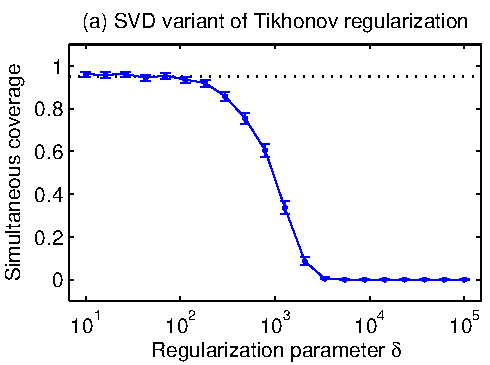
\includegraphics[width=0.5\linewidth]{figures/chapter-02/incJets_lumFactor150nBinsE30nBinsF30JointCoverageSVD.pdf}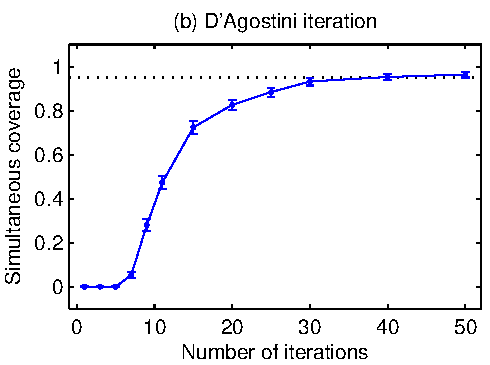
\includegraphics[width=0.5\linewidth]{figures/chapter-02/incJets_lumFactor150nBinsE30nBinsF30JointCoverageDAgostini.pdf}
                \caption[Coverage properties of Tikhonov regularisation and IBU]{Coverage of 95\% confidence intervals with Tikhonov regularisation (left) and IBU (right).
                %
                The error bars are given by the 95\% Clopper–Pearson intervals and the nominal confidence level is shown by the dotted line.
                %
                When the regularization is strong (fewer iterations in the case of IBU), both methods undercover substantially. IBU~\cite{kuusela_shape-constrained_2017}}
                \label{fig:coverage}
            \end{figure}
    \subsubsection{Variance and bias decomposition}
        The total error of an unfolding method can be decomposed into bias and variance components,
        \begin{equation}
        \text{MSE}(\hat{t}) = \text{Bias}^2(\hat{t}) + \text{Var}(\hat{t}),
        \end{equation}
        where \(\text{Bias}(\hat{t}) = \mathbb{E}[\hat{t}] - t\) and \(\text{Var}(\hat{t}) = \mathbb{E}[(\hat{t} - \mathbb{E}[\hat{t}])^2]\). 
        
        This decomposition is particularly valuable for understanding the trade--offs inherent in regularized unfolding methods, where stronger regularization typically reduces variance at the expense of increased bias.
        %
        Different applications might prioritize minimizing one component over the other, making this decomposition essential for method selection.

    \subsection{Evaluation of correlation structure}
        Traditional evaluation metrics often focus on marginal distributions, overlooking an important aspect of unfolding: the correlation structure between different bins or events.
        %
        Properly accounting for these correlations is crucial for downstream analyses.
        \subsubsection{Covariance Matrix Assessment}
            For binned methods, the full covariance matrix of the unfolded distribution provides information about bin--to--bin correlations.
            %
            A useful measure is the correlation matrix, defined as
            \begin{equation}
                \text{Corr}_{ij} = \frac{\text{Cov}_{ij}}{\sqrt{\text{Cov}_{ii}\text{Cov}_{jj}}}
            \end{equation}
            Comparing the correlation structure of the unfolded distribution to that of the true distribution (when known, e.g. in simulation studies) can reveal systematic distortions introduced by the unfolding procedure.
        \subsubsection{Event--to--event correlation metrics}
            For unbinned methods event--to--event correlations in the unfolded weights can significantly impact downstream inference.
            %
            These correlations can be quantified by studying the weight correlation as a function of distance.
            %
            For any pair of events, one can compute the correlation between their weights as a function of their distance in feature space.
            %
            One can also estimate the reduction in statistical power due to correlated weights
            \begin{equation}
                \label{eq:n-eff}
                N_{\text{eff}} = \frac{\left(\sum_{i} w_i\right)^2}{\sum_{i} w_i^2 + 2\sum_{i<j} w_i w_j \text{Corr}(w_i, w_j)}
            \end{equation}
            In this equation, \(N_{\text{eff}}\) represents the effective number of independent observations when event weights are correlated, derived from the variance properties of weighted sums.
            %
            The numerator, \(\qty(\sum w_i^2)\) represents the square of the total weighted sample size.
            %
            The denominator consists of two components, which together account for the increased variance introduced by weight correlations.
            %
            The first term, \(\sum w_i^2\), captures the variance contribution from individual event weights, similar to the standard effective sample size formula for independent weighted observations.
            %
            The second term, \(2\sum_{i<j} w_i w_j \operatorname{Corr}(w_i, w_j)\), accounts for the covariance contributions between all pairs of events, where the factor of 2 arises because each pair appears only once in the sum over \(i<j\).

            When weights are uncorrelated, \(\operatorname{Corr}(w_i, w_j) = 0,\) and the formula reduces to the familiar \(N_{\text{eff}}=\nicefrac{\qty(\sum w_i)^2}{\sum w_i^2}.\)
            %
            However, upon unfolding methods, nearby events in phase space often receive similar weight corrections\footnote{as will be discusseed in greater detail in \cref{chap:unbinned_correlations}}, leading to correlations that increase the denominator and reduce the effective sample size.
            %
            This reduction quantifies the loss of statistical power compared to an ideal scenario with independent weights.

            The formula emerges from considering the variance of weighted observables.
            %
            For a weighted sum, \(S = \sum w_i\,x_i\), the variance is
            \[
                \operatorname{Var}(S) = \sum_i \sum_j w_i w_j \operatorname{Cov}(x_i, x_j),
            \]
             which is the denominator of the \cref{eq:n-eff}.
             %
             The effective sample size is then defined as the ratio of the squared expectation to the variance, providing a measure of statistical efficiency that accounts for both weight magnitudes and their correlations.
             
            \cref{fig:corr-decay} illustrates how event correlations typically decay with distance, with the correlation length scale increasing with detector resolution effects.
            \begin{figure}
                \centering
                \includegraphics[width=\linewidth]{figures/chapter-02/weight-correlation-vs-distance-1d-set1.pdf}
                \caption[Weight correlation between event pairs as a function of distance between events.]{Average weight correlation between two events as a function of the absolute distance between the events in the observable for Gaussian data unfolded using \textsc{OmniFold}~\cite{Desai:2025mpy}.\protect\footnotemark
                }
                \label{fig:corr-decay}
            \end{figure}
            \footnotetext{Figure created by Owen Long}
    \subsection{Method specific evaluation metrics}
        \subsubsection{Iterative methods}
            For iterative methods like Iterative Bayesian Unfolding (IBU) or \textsc{OmniFold}, convergence behaviour provides important diagnostic information.
        %
        To study the convergence behaviour, we plot metric values (e.g., \(\chi^2\) or NLL) as a function of iteration number.
        %
        We then compare unfolded distributions at different iterations to assess stability and analyse how the bias--variance trade off evolves with iteration number.

        \subsubsection{Bayesian Methods}
            For Bayesian unfolding methods such as Fully Bayesian Unfolding (FBU)~\cite{choudalakis_fully_2012} or Neural Posterior Unfolding (NPU)~\cite{acosta2024npu}, additional posterior specific metrics are relevant.
            %
            We can compare detector level data to detector level predictions generated from the posterior.
            %
            We assess convergence using standard MCMC based diagnostics like Gelman--Rubin statistics or effective sample size.
            %
            The width of the posterior allows us to evaluate the posterior uncertainty in relation to the true frequentist variance.

    \subsection{Practical considerations.}
        In general, when comparing different unfolding methods, a structured evaluation framework ensures fair and comprehensive assessment. Such a framework should consider
        \begin{itemize}
            \item Computational efficiency: Measure training time, inference time, and memory requirements.
            \item Dimensionality scaling: Assess how performance metrics change as the dimensionality of the problem increases.
            \item Prior dependence: Evaluate robustness to different initial simulations.
            \item Regularisation parameter sensitivity: Compare how performance varies with changes in regularization strength.
        \end{itemize}

        In real experimental settings where the truth is unknown, evaluation presents additional challenges that require alternative pragmatic approaches.
        %
        For example, when the true distribution is unavailable, data-splitting techniques can provide useful validation.
        %
        The two most commonly used techniques are cross-validation, where we split the detector--level data, unfold one portion, then refold it, and compare predictions against the held--out portion; and bootstrapping where we generate multiple resampled datasets to assess the stability of the unfolding procedure.

        Closure tests involve applying the full analysis chain (forward model followed by unfolding) to a known input distribution.
        %
        While not a direct evaluation of performance on real data, closure tests provide confidence in the methodology.
        %
        The simplest kinds of closure tests involve apply detector simulation to a known particle--level distribution, then unfolding the resulting detector--level distribution and compare with the original input.
        %
        This procedure can then be modified by using a different particle-level input than the one used to train the unfolding method, testing robustness to prior misspecification.
        
        Evaluating how unfolding methods propagate systematic uncertainties is crucial for real-world applications.
        %
        We can test the sensitivity of the method to systematic uncertainties by applying variations to the response matrix based on known systematic uncertainties and assessing the impact on unfolded distributions.
        %
        For methods that support nuisance parameter profiling, evaluating how effectively nuisance parameters are profiled out is a gold standard test for the effectiveness of the method.
        
        Rigorous evaluation of unfolding methods requires a multi--faceted approach that considers accuracy, uncertainty quantification, and computational performance.
        %
        The metrics and frameworks presented in this section provide a comprehensive foundation for assessing both traditional and machine learning-based unfolding techniques.
        %
        For binned methods, established metrics like \(\chi^2\) and coverage tests remain valuable, while for unbinned approaches, distributional metrics like Wasserstein distance and VLC divergence offer more appropriate evaluation.
        %
        Regardless of the method, uncertainty calibration through pull distributions and correlation structure assessment are important to validate any measurement.
        %
        As unfolding methods continue to evolve, particularly with the advent of machine learning approaches, evaluation metrics must adapt accordingly.
        %
        The framework presented here is designed to be extensible, accommodating new methods and application domains while maintaining rigour and comparability
\chapter{Machine Learning for Unfolding}
\label{chap:ml-for-unfolding}
\section{The Emergence of Machine Learning in Particle Physics}
\subsection{A Paradigm Shift in Data Analysis}
The past decade has witnessed a remarkable transformation in how particle physicists analyse data, driven by the adoption and adaptation of machine learning (ML) techniques.
%
This revolution has been catalysed by the confluence of three factors: the growing volume and complexity of data from modern collider experiments, the substantial increase in available computing resources, and the rapid advancement of ML algorithms and frameworks.
%
The Large Hadron Collider (LHC) alone produces petabytes of data annually, with individual collisions generating thousands of particles across multiple detector subsystems, creating a rich, high dimensional dataset that traditional analysis methods struggle to fully exploit~\cite{EnvironmentalCERN}.
%
Particle physics presents unique analytical challenges that align particularly well with the strengths of modern machine learning approaches.
%
The field routinely deals with high--dimensional feature spaces, complex non--linear correlations between observables, rare signal processes buried within overwhelming backgrounds, and some of the largest scientific datasets in existence~\cite{DiMeglio2017SubmitterResearch}.
%
These characteristics create an ideal test bed for advanced ML techniques, which excel at discovering patterns in precisely such environments.
%

The relationship between particle physics and machine learning is not entirely new.
%
Neural networks were first applied to high energy physics problems in the late 1980s and 1990s~\cite{Teodorescu2008ArtificialPhysics}.
%
However, these early applications were limited by computational resources and algorithmic capabilities.
%
The contemporary renaissance began around 2012--2014, coinciding with the broader deep learning revolution across computer science~\cite{TerrenceJ.Sejnowski2018TheIntelligence}.
%
This timing allowed particle physicists to leverage developments in computer vision, reinforcement learning, and generative modelling, adapting these techniques to the unique requirements of high-energy physics.
\subsection{Evolution of ML Applications in HEP}
\subsubsection{Classification Tasks}
        \label{subsubsec:classification-tasks}
The first wave of modern ML applications in particle physics focused predominantly on classification tasks, particularly signal/background discrimination and particle identification.
%
These problems are naturally framed as binary or multi--class classification, making them accessible entry points for machine learning techniques.
%
Boosted decision trees initially dominated these applications, particularly in the analysis chains that led to the Higgs boson discovery~\cite{Chen2014HiggsTrees}.
%
However, deep neural networks quickly demonstrated superior performance by automatically discovering complex patterns in high--dimensional data, often outperforming carefully hand--crafted physics--inspired variables~\cite{Baldi2014SearchingLearning, Baldi2015EnhancedLearning, Baldi2021DeepScience}.
%
For example, neural networks trained on low--level detector information have been shown to match or exceed the performance of approaches using physics--motivated high--level features for tasks like quark--gluon discrimination~\cite{Lee2019Quark-GluonNetworks} and top quark tagging~\cite{Pearkes2017JetTagging}
%
The ATLAS and CMS experiments have now incorporated deep learning based taggers for identifying hadronically decaying W/Z bosons~\cite{Chen2020BoostedLearning}, top quarks~\cite{Sirunyan_2020}, and Higgs bosons~\cite{2023TransformerATLAS}, significantly enhancing their sensitivity to new physics.
%
While early applications leveraged convolutional neural networks to exploit spatial correlations in calorimeter deposits~\cite{deOliveira2016Jet-imagesEdition, Komiske2018DeepDiscrimination} and recurrent or graph neural networks to handle variable--length, unordered collections of particles~\cite{Shlomi2020GraphPhysics, Qu2020ParticleNet:Clouds}, transformer architectures and foundation models have emerged as the current state of the art for many classification tasks~\cite{Qu2022ParticleTagging, Mikuni2025SolvingModels, VanStroud2024TransformersPhysics}.
%
Transformers excel at modelling complex dependencies through self--attention mechanisms, naturally processing sets of particles by capturing relationships between a span of pairs of particles simultaneously~\cite{Vaswani2017AttentionNeed}.
%
The Particle Transformer (ParT) architecture~\cite{Qu2022ParticleTagging}, specifically designed for HEP applications, has demonstrated superior performance on jet classification tasks by incorporating physics-motivated constraints while leveraging the power of self-attention to identify relevant particle interactions and correlations~\cite{Wang2024InterpretingTagging}.

\subsubsection{Regression and Anomaly Detection}
        \label{subsubsec:regression-and-anomaly-detection}
As the field matured, ML applications expanded beyond classification to include regression tasks, such as energy calibration~\cite{Holmberg2023JetPipeline}, pileup mitigation~\cite{Komiske2018PileupPUMML}, and particle momentum reconstruction~\cite{Haake2019Machine-learning-basedCollisions}.
%
These applications require models to predict continuous quantities rather than discrete classes, introducing additional complexity but extending ML based methods to a larger class of problems.
%
Simultaneously, unsupervised and weakly--supervised learning techniques emerged as powerful tools for anomaly detection, identifying potential new physics without explicit models~\cite{Belis2024MachinePhysics}.
%
These methods include autoencoders that flag events with high reconstruction loss, density estimation techniques that identify low--probability regions of phase space, and weakly--supervised classifiers that can distinguish data mixtures without event--by--event labels.

\subsubsection{Generative Models}
Perhaps the most significant recent development in ML for HEP has been the adoption of generative models, which learn to produce samples from complex probability distributions.
%
This capability is particularly valuable in particle physics, where accurate simulation is crucial but computationally expensive.

Generative adversarial networks (GANs)~\cite{Goodfellow2014GenerativeNetworks}, variational autoencoders (VAEs)~\cite{Kingma2019AnAutoencoders}, and normalizing flows~\cite{Kobyzev2019NormalizingMethods} have all been successfully applied to particle physics problems.
%
These models can generate synthetic collision events\cite{Moodie2022OptimisingNetworks}, simulate detector responses\cite{Darulis2022MachineSimulations, Xu2023GenerativeFlow}, and model complex differential distributions,\cite{Butter2025GenerativeMapping} often accelerating these processes by orders of magnitude compared to traditional Monte Carlo techniques.

The development of these generative models opened new possibilities for addressing inverse problems in particle physics, including the unfolding problem at the centre of this dissertation.
%
By learning complex, high--dimensional probability distributions directly from data, these methods offer a natural framework for tackling unfolding without the limitations of binning.

\subsection{Machine Learning Approaches to Unfolding}

The application of machine learning to unfolding represents a particularly promising frontier.
%
Traditional unfolding methods face significant challenges when dealing with high--dimensional spaces, correlated variables, and complex detector effects.
%
Machine learning approaches offer several potential advantages compared to traditional statistical methods.

Neural networks excel at capturing patterns in high-dimensional spaces, helping to mitigate the curse of dimensionality that plagues binned methods.
%
While traditional approaches become computationally prohibitive beyond a few dimensions, ML-based methods can effectively unfold many variables simultaneously`~\cite{komiske_preserving_2021}.
%
This capability enables jointly unfolding multi--differential measurements that would be impractical with conventional techniques.

Many ML--based unfolding methods operate directly on continuous distributions, eliminating binning bias and the need to predetermine bin boundaries.
%
This approach preserves fine--grained information that might otherwise be lost through discretization, and it enables the extraction of arbitrary derived observables from the unfolded distribution~\cite{Shmakov2025FullDiffusion}.
%
Furthermore, the architecture and training procedure of neural networks provide natural regularization without requiring explicit constraints.
%
Rather than manually tuning regularization parameters as in traditional methods, ML approaches incorporate regularization through network depth, width, dropout rates, and early stopping~\cite{Girosi1995RegularizationArchitectures}.
%
This implicit regularization can adapt more naturally to the varying complexity across different regions of phase space.

Additionally, some ML methods can learn the complete detector--to--particle transformation in a single training procedure, avoiding the separate steps of response matrix estimation and inversion required by traditional approaches.
%
This integrated optimization may reduce the compounding of uncertainties that can occur when errors propagate through multiple discrete stages of conventional unfolding pipelines
%
Once trained, many ML models also enable rapid inference on new data without retraining.
%
This amortized approach is particularly valuable for unfolding tasks that need to be repeated with slight variations, such as systematic uncertainty studies or detector condition changes~\cite{Brehmer2020EffectiveLearning}

    \subsection{Early successes and current challenges}
        Machine learning approaches to unfolding, such as \textsc{OmniFold}, have demonstrated promising results on jet substructure measurements, showing improved performance in high dimensional spaces compared to traditional methods.
        %
        \textsc{OmniFold} has been successfully applied in experimental analyses at H1~\cite{collaboration_measurement_2022, collaboration_unbinned_2023, collaboration_machine_2024, Arratia2025TowardsEvents}, STAR~\cite{song_measurement_2023, pani_generalized_2024}, T2K~\cite{Huang2025MachineTechnique}, ATLAS~\cite{collaboration_simultaneous_2024, collaboration_measurement_2025}, CMS~\cite{collaboration_measurement_2025}, and LHCb~\cite{collaboration_multidifferential_2023}, validating its practical utility.
        %
        However, these methods also face significant challenges.
        %
        Unlike traditional techniques with decades of validation, ML--based unfolding is relatively new and requires careful validation to ensure physical consistency.
        %
        Key concerns include proper uncertainty quantification, interpretability of the results, sensitivity to the training data, and potential biases introduced by the neural network architecture or training process~\cite{mishra_uncertainty_2021}.
        %
        Additionally, the field is still developing consensus on best practices for hyperparameter selection, architecture design, and evaluation metrics specific to unbinned unfolding.
        %
        The balance between flexibility and stability remains an active area of research, with new approaches continuing to emerge.

        As machine learning continues to evolve, both within particle physics and in the broader scientific community, we can expect further innovations in unfolding techniques.
        %
        Promising directions include physics--informed neural networks that incorporate known conservation laws or symmetries~\cite{raissi_physics-informed_2019}, uncertainty--aware models that provide more reliable error estimates~\cite{brehmer_guide_2018}, and techniques that combine the strengths of traditional and ML based approaches~\cite{willard_integrating_2022}.
        %
        The rapid progress in this field demonstrates the synergistic relationship between particle physics and machine learning.
        %
        Particle physics provides challenging problems and unique datasets that drive methodological innovations;
        %
        machine learning offers powerful tools that enable new measurements and insights.
        %
        This dissertation builds upon this foundation, exploring novel machine learning approaches to improve the precision and scope of differential cross--section measurements through novel unfolding techniques.

\section{Introduction to Neural Networks}
Neural networks are the fundamental building blocks of modern machine learning applications.
%
This section provides a rigorous mathematical framework for understanding neural networks, from their basic architecture to training methodologies.

    \subsection{Essential Concepts}
        \subsubsection{Neural Network Fundamentals}
            At its core, a neural network is a parametric function approximator loosely inspired by biological neural systems.
            %
            The fundamental unit, a neuron or node, computes a weighted sum of its inputs followed by a non-linear transformation:
            \begin{equation}
            y = \sigma(w^T x + b)
            \end{equation}
            where \(x \in \mathbb{R}^n\) is the input vector, \(y\in\R^{m}\) is the output vector, \(w \in \mathbb{R}^{n\times m}\) is a weight matrix, \(b \in \mathbb{R}^m\) is a bias term, and \(\sigma(\cdot)\) is a (typically non--linear) activation function.
            
            The \emph{depth} of a neuron is defined as the length of the longest path between the input and the neuron.
            %
            The set of all neurons at depth \(l\) is called \emph{layer} \(l\) of the network.
            %
            The width of a layer is the number of neurons in that layer.
            %
            This organization of neurons into layers, creates a hierarchical structure.
            %
            The \emph{depth}, \(d = l_{\max}\), of a neural network is defined as the depth of its deepest layer.
            %
            A graphical overview of these concepts is depicted in \cref{fig:nn-concepts}.
            \begin{figure}
                \centering
                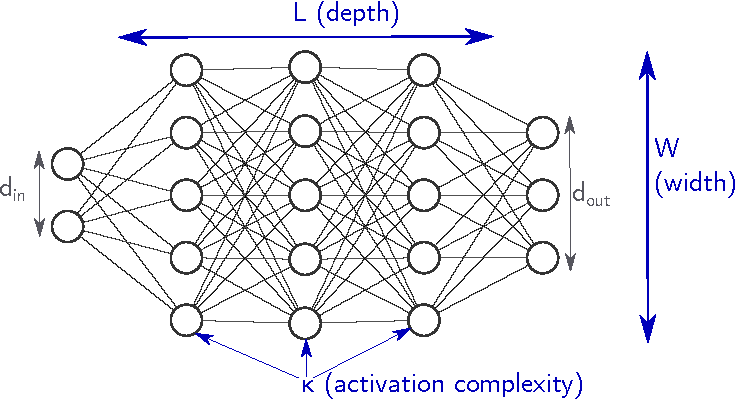
\includegraphics[width=\linewidth]{figures/chapter-03/CPWLNet_Descriptor.pdf}
                \caption[Neural network depth & width illustration]{Diagram illustrating the key structural parameters of a neural network: depth (number of layers), width (units per layer), and their relationship to input, hidden, and output layers~\cite{goujon_number_2023}.}
                \label{fig:nn-concepts}
            \end{figure}
            Any layer of a neural network except the input layer (often labelled layer \(0\)) and the output layer (\(l_{\max})\) is called a hidden layer.
            %
            A \emph{deep neural network} is a neural network with depth, \(d > 2\).
            %
            That is to say standard deep feed forward neural network consists of an input layer, \emph{more than one} hidden layers, and an output layer.%
            
            \cref{fig:shallow-nn} depicts a shallow neural network comprising a single hidden layer, while \cref{fig:deep-nn} shows a deep neural network with multiple hidden layers.
            %
            The shallow architecture can model only a limited set of simple, low level features, whereas the deep architecture composes successive non-linear transformations to extract increasingly abstract representations.
            %
            Increasing depth enhances representational capacity of the network and its capacity for hierarchical feature learning, albeit at the cost of greater computational complexity and potential optimization challenges.

            \newlength{\subfigheight}
            \setlength{\subfigheight}{4cm}
            \begin{figure}
              \centering
              \begin{subfigure}[b]{0.4\textwidth}
                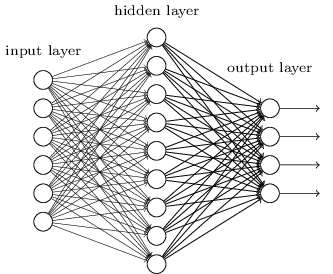
\includegraphics[height=\subfigheight,keepaspectratio]{figures/chapter-03/tikz35.png}
                \caption{Shallow network}
                \label{fig:shallow-nn}
              \end{subfigure}
              \begin{subfigure}[b]{0.5\textwidth}
                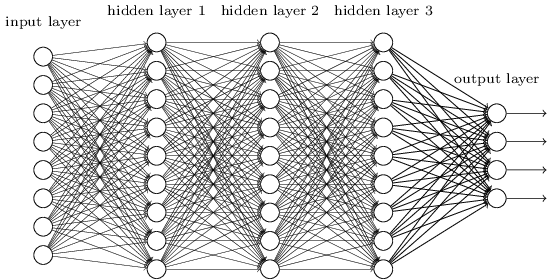
\includegraphics[height=\subfigheight,keepaspectratio]{figures/chapter-03/tikz36.png}
                \caption{Deep network}
                \label{fig:deep-nn}
              \end{subfigure}
              \caption[Shallow vs.\ deep NN]{Comparison between a shallow neural network (left) with a single hidden layer and a deep neural network (right) with multiple hidden layers~\cite{nielsen_neural_2015}.}
              \label{fig:shallow-deep}
            \end{figure}

            
            For a network with \(d\) layers, at each layer \(l\) the neural network computes
            \begin{equation}
                y^{(l)} = \sigma^{(l)}(W^{(l)} y^{(l-1)} + b^{(l)})
            \end{equation}
            where \(y^{(l)}\) represents the output of layer \(l, W^{(l)}\) is the weight matrix, \(b^{(l)}\) is the bias vector, and \(\sigma^{(l)}\) is the activation function of later \(l\).
            %
            By convention, \(y^{(0)} = x\) is the input, and \(y^{(d)} = y\) is the output.

            This architecture enables neural networks to approximate arbitrarily complex functions, as formalized in the Universal Approximation Theorem, which states that a deep neural network containing a finite number of neurons can approximate any continuous function on compact subsets of \(\mathbb{R}^n\) given certain mild conditions on the activation function.
            %
            Importantly, neural networks achieve superior approximation rates compared to traditional methods like polynomials, particularly in high dimensional settings.
            %
            While polynomial approximation suffers from the curse of dimensionality, requiring $\mathcal{O}(\varepsilon^{-d})$ parameters to achieve accuracy $\varepsilon$ in $d$ dimensions, neural networks can approximate smooth functions with rates of $\mathcal{O}(n^{-r/d})$ where $n$ is the number of parameters and $r$ is a smoothness parameter, often with significantly better constants and the ability to exploit compositional structure in the target function~\cite{petersen_optimal_2018,lu_expressive_2017}.

        
        \subsubsection{Forward propagation}
            The process of computing the network's output given an input is called forward propagation.
            %
            From its input \(y^{(0)} = x\) the network sequentially computes the output of each layer
            \begin{align}
                z^{(1)} &= W^{(1)}y^{(0)} + b^{(1)} \\
                y^{(1)} &= \sigma^{(1)}(z^{(1)}) \\
                &\nonumber \vdots \\
                z^{(d)} &= W^{(d)}y^{(d-1)} + b^{(d)} \\
                y^{(d)} &= \sigma^{(d)}(z^{(d)})
            \end{align}
            where \(z^{(l)}\) represents the pre--activation values at layer \(l\).
            %
            \cref{fig:forward-pass} depicts the computation in the forward pass.
            %
            Successive layer activations are computed by applying the weight matrices and bias vectors to the input, then passing the result through each layer's non-linear activation function until the final output is produced.
            \begin{figure}
                  \centering
                  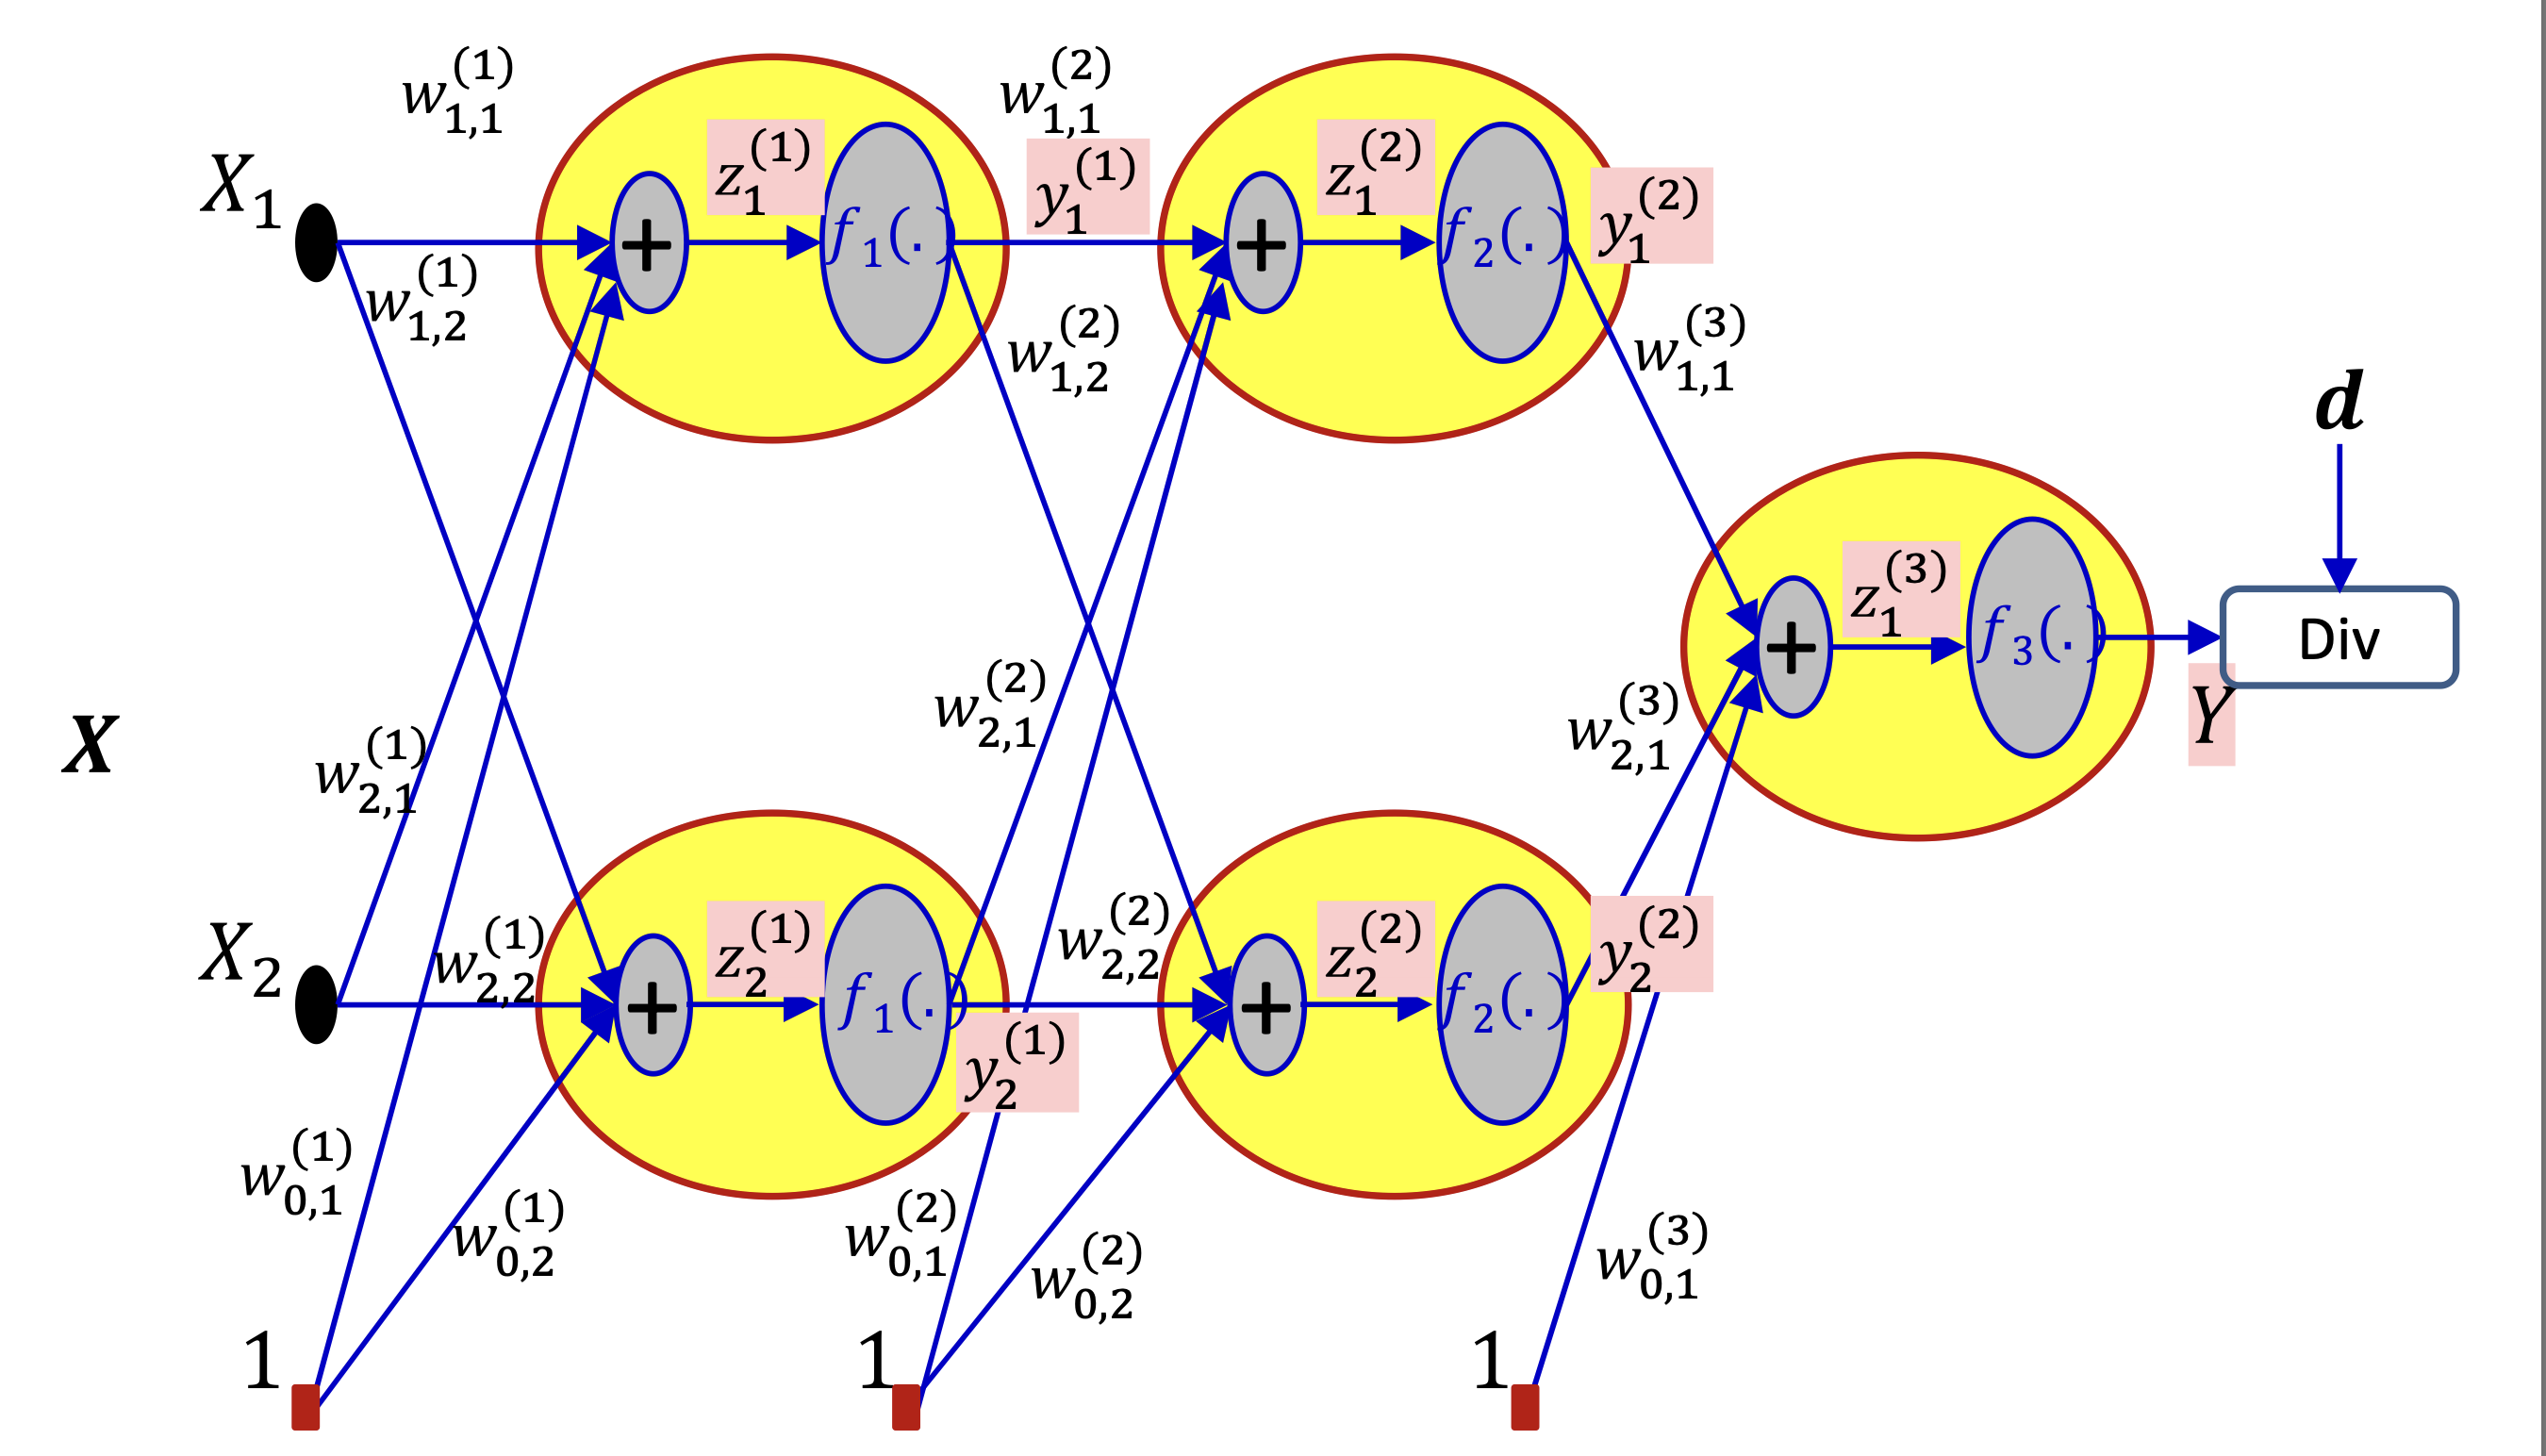
\includegraphics[width=0.8\textwidth]{figures/chapter-03/forwardpass.png}
                  \caption[Forward pass]{Illustration of the forward propagation process in a neural network, showing how the input vector is transformed by each layer's weights and biases and then passed through non-linear activation functions to yield the final output~\cite{noauthor_idl_nodate}.}
                  \label{fig:forward-pass}
            \end{figure}
        \subsubsection{Training objectives and loss functions}
            In order to quantify the accuracy with which a neural network \(f\) models a desired target function \(g\) for any particular input \(x\), a suitable measure of the error between \(f(x)\) and \(g(x)\) is required.
            %
            The \emph{divergence} \(\operatorname{Div}(x)\) is a continuous valued proxy for this error.
            %
            The goal of training can then be defined to be to learn the values of \(W\) that minimize the expected divergence.
            %
            (For notational convenience, from here on out, \(b\) will be collapsed into \(W\) as its \(0^{\textrm{th}}\) column;
            %
            the corresponding input, \(x_0 = 1\).)
            \begin{equation}
                \widehat{W} = \underset{W}{\arg\min}\int_X \operatorname{Div}\Big(f(x;\,W), g(x)\Big)\;p_X(x)\;\dd x
            \end{equation}

            In practice however, \(g\) is often not known for all \(x\in X,\) it is only known at some subset \(\qty{x_i}\subseteq X\).
            %
            The \emph{Loss function} \(\mathcal{L}\) is defined as the unbiased empirical average divergence between the neural network output and the target output over all training instances.
            \begin{equation}
                \mathcal{L}(W) = \frac{1}{N_X}\sum_{i=1}^{N_X}\operatorname{Div}\Big(f(x_i;\,W), g(x_i)\Big).
            \end{equation}
            The expected value of the loss function can be proved to be the expected divergence, which is precisely what it means for the loss function to be an unbiased estimate of the expected divergence.
            %
            However, this does not guarantee that minimizing the loss function will minimize the expected divergence.
        \subsubsection{Backpropagation and parameter learning}
            The training of neural networks revolves around finding the optimal values for weights and biases that minimize the loss function \(\mathcal{L}\)
            %
            Backpropagation is the algorithm used to efficiently compute gradients of the loss function with respect to each network parameter.
            %
            The core idea of backpropagation relies on the chain rule of calculus.
            %
            For a loss function \(\mathcal{L}\) and parameters \(\{W^{(l)}\}_{l=1}^d\) the network computes
            \begin{equation}
            \frac{\partial \mathcal{L}}{\partial W^{(l)}} = \frac{\partial \mathcal{L}}{\partial z^{(l)}} \frac{\partial z^{(l)}}{\partial W^{(l)}} = \delta^{(l)} (y^{(l-1)})^T 
            \end{equation}
            
            where \(\delta^{(l)} = \frac{\partial \mathcal{L}}{\partial z^{(l)}}\) is the error term for layer \(l\).
            %
            These error terms are computed recursively, starting from the output layer.
            \begin{align}
                \delta^{(L)} &= \frac{\partial \mathcal{L}}{\partial y^{(L)}} \odot \sigma'^{(L)}(z^{(L)}) \\
                \delta^{(l)} &= ((W^{(l+1)})^T \delta^{(l+1)}) \odot \sigma'^{(l)}(z^{(l)})
            \end{align}
            where \(\odot\) denotes the Hadamard (element-wise) product and \(\sigma'\) is the derivative of the activation function.
            %
            These derivatives are thus propagated backwards through the network, beginning at the output layer, propagated to the input layer.

        
        \subsubsection{Batching and Training Dynamics}
            In practice, neural networks are trained using mini--batch gradient descent, where parameter updates are performed using gradients computed on subsets (batches) of the training data. For a batch of size \(B\), the loss is
            \begin{equation}
                \mathcal{L}_{\text{batch}} = \frac{1}{B}\sum_{i=1}^B\mathcal{L}(x_i, y_i, W)
            \end{equation}
            Training proceeds in \emph{epochs}, where each epoch represents one complete pass through the training dataset.
            %
            To prevent overfitting, a separate validation dataset is typically used to monitor performance, and techniques such as early stopping may be applied when validation performance plateaus or degrades.
    \subsection{Neural Networks as Universal Approximators}
        The power of neural networks in physics applications stems from their ability to approximate arbitrary functions without requiring exponentially many parameters, unlike traditional methods such as polynomial approximation which suffer from the curse of dimensionality.
        %
        This property is formalized in the Universal Approximation Theorem, which has several variations but fundamentally states that feed-forward networks with a single hidden layer can approximate any continuous function on compact subsets of \(\mathbb{R}^n\) to arbitrary precision, given sufficient depth and width.
        \begin{theorem}[Universal Approximation Theorem]
        \begin{align}
            &\forall \sigma\in C^0(\R)\; \forall g\in C^0([0, 1]^n)\;\forall\epsilon > 0\;\exists M\in \R\\
            &\Bigg[\forall x\in\R\;|\sigma(x)| < M\implies \exists N\in\mathbb{N}\;\exists c, b\in \R^N\;\exists W\in \R^{N\times n}\\
            &\Big\{\forall z\in[0, 1]^n |c^T\sigma(Wz + b) - f(z)|<\epsilon\Big\} \lor \exists A\in\R\;\forall x\in\R\;\sigma(x) = A\Bigg].
            \end{align}
        \end{theorem}
        This theorem was first proved by Cybenko for sigmoid activation functions~\cite{cybenko_approximation_1989} and later extended by Hornik et. al to include a broader class of activation functions~\cite{hornik_multilayer_1989}. Modern versions of the theorem have relaxed various assumptions and expanded the results to deeper networks~\cite{augustine_survey_2024}.
        \subsubsection{Relevance to physics applications}
            The universal approximation property is particularly significant in physics.
            %
            Many physical systems are governed by complex, non-linear differential equations that lack closed-form solutions.
            %
            Neural networks can approximate these solutions without explicitly knowing the underlying equations, hence serving as excellent implicit simulators.
            %
            Additionally, physics problems often involve high dimensional spaces\footnote{e.g., the phase space for jet physics}.
            %
            Neural networks excel at learning in such spaces, where traditional numerical methods become computationally intractable.
            %
            The universal approximation property makes neural networks well--suited for these tasks, where the mappings to be learned are highly complex.

            When theoretical descriptions are incomplete, neural networks can discover patterns in data that suggest new physical models or refinements to existing ones.
            %
            Neural networks as universal approximators are also helpful for simulation based inference.
            %
            Modern physics often relies on computer simulations rather than closed--form likelihood functions.
            %
            Neural networks can approximate these implicit models for fast posterior inference.

            While the Universal Approximation Theorem guarantees the existence of a neural network capable of approximating any continuous function, it does not provide guidance on architecture design or training procedures.
            %
            Nor does the theorem provide any guarantees about the rate of convergence of training procedures.
            %
            In practice, deeper networks with multiple hidden layers have provide faster convergence, and greater parameter efficiency as discussed above.
            %
            However, the benefits of increasing depth are bounded, and decay exponentially, and hence the choice of architecture can involve carefully balancing the increased computational cost of a deeper network with the gains it provides.
            %
            Extensions of the theorem show that depth can exponentially reduce the number of neurons required to approximate certain function classes, explaining the empirical success of deep learning in physics applications.
            %
            These theoretical insights have motivated the development of specialized architectures tailored to specific physics problems, as will be discussed in subsequent sections.
    \subsection{Activation Functions, Optimization, and Regularization}
        \subsubsection{Activation Functions}
            Activation functions introduce non--linearity into neural networks, enabling them to learn complex patterns.
            %
            Several activation functions are commonly used in high energy physics applications.
            \begin{itemize}
                \item Sigmoid:
                    \[\sigma(z) = \frac{1}{1 + e^{-z}}\]
                    An activation function that outputs values between \(0\) and \(1\), it is most often used in problems involving binary classification.
                    %
                    The sigmoid activation function has a rich and important history as one of the earliest activation functions to be used in machine learning applications.
                    %
                    However, it suffers from vanishing gradient problems, where training instances far from its inflection point do not provide much information to the system.
                    %
                    Additionally, when many sigmoid functions are composed in deep networks, the resulting function can become very sharp and step--like, leading to training instabilities and poor gradient flow.

                \item Hyperbolic Tangent (tanh): \[\tanh(z) = \frac{e^z - e^{-z}}{e^z + e^{-z}}\]
                    The hyperbolic tangent function is very similar to sigmoid, except that it outputs values between \(-1\) and \(1\).
                    %
                    It is preferred in some applications because it is zero--centered, which can help in training dynamics, but it also suffers from the same vanishing gradient problems as the sigmoid.
                \item Rectified Linear Unit (ReLU): \[\text{ReLU}(z) = \max(0, z)\]
                    Simple, and incredibly computationally efficient, ReLU has become one of the most frequently used activation functions both within HEP and in the AI/ML space more broadly.
                    %
                    It addresses the vanishing gradient problem for positive inputs.
                    %
                    However, since it is simply zero for half its support, it can suffer from the ``dying ReLU" problem where units can become permanently inactive.
                \item Leaky ReLU: \[\text{LeakyReLU}(z) = \max(\alpha z, z)\]
                    \(\alpha\) is a small positive constant.
                    %
                    LeakyReLU is a modification of ReLU to allow small negative valued outputs~\cite{Maas2013RectifierModels}, which helps mitigate the dying ReLU problem.
                    %
                    Just a few of the many other variants that exist include Parametric ReLU (PReLU)~\cite{he_delving_2015} where \(\alpha\) is learnable, Exponential Linear Unit (ELU)~\cite{clevert_fast_2016} which provides smooth transitions for negative inputs, and Gaussian Error Linear Unit (GELU)~\cite{hendrycks_gaussian_2023} which has become popular in modern transformer architectures.

                \item Softmax: \[\text{softmax}(z_i) = \frac{e^{z_i}}{\sum_{j} e^{z_j}}\]
                        Softmax is most often used for multi--class classification output layers because it produces a probability distribution over classes.
                        %
                        The softmax reduces to the sigmoid when there only two classes, rendering binary classification simply a special case of multi--class classification.
            \end{itemize}
            These a but a few examples of the most common activation functions.
            %
            The choice of activation function significantly impacts network performance, convergence speed, and the occurrence of issues like vanishing or exploding gradients.
        \subsubsection{Optimization Techniques}
            As we discussed, neural network training is fundamentally an optimization problem.
            %
            Various algorithms have been developed to find optimal parameters efficiently.
            
            \paragraph{Gradient Descent}is the oldest and simplest approach to optimization.
            %
            It involves updating parameters in the direction of the negative gradient:
           \begin{equation}
                W_{t+1} = W_t - \eta \nabla_W \mathcal{L}(W_t)
           \end{equation}
            \(\eta\) is the learning rate.
            %
            While conceptually simple, gradient descent can be slow to converge and may get trapped in suboptimal solutions such as local minima.
            
            \paragraph{Stochastic Gradient Descent (SGD)}is an adaptation of gradient descent that updates parameters using gradients computed on mini--batches, introducing noise that can help escape local minima.
            \begin{equation}
            W_{t+1} = W_t - \eta \nabla_W \mathcal{L}_{\text{batch}}(W_t)
            \end{equation}
            \paragraph{Momentum based methods}accelerate convergence by accumulating a ``velocity" vector in directions of persistent reduction in the loss function.
               \begin{align}
                   v_{t+1} &= \gamma v_t + \eta \nabla_W \mathcal{L}(W_t) \\
                   W_{t+1} &= W_t - v_{t+1}
               \end{align}
               where \(\gamma\) is the momentum coefficient.
               %
               In HEP applications, a typical value of \(\gamma\) is \(0.9\).
            
            \paragraph{Adaptive Methods}are methods that vary the learning rate \(\eta\) over the course of the training rather than keeping it constant, and allow different learning rates for different dimensions of the input, rather than the traditional scalar learning rate that was constant across dimensions.
                \subparagraph{AdaGrad}
                    One of the earliest adaptive methods proposed was AdaGrad~\cite{duchi_adaptive_nodate}, which adapts learning rates per-parameter based on historical gradients.
                    %
                    AdaGrad was however limited by its aggressive learning rate reduction that slowed down training considerably.
                \subparagraph{RMSProp}
                    AdaGrad was soon replaced in almost all applications by RMSProp~\cite{hinton_neural_nodate}, an unpublished algorithm proposed by Hinton in course lectures~\cite{ruder_overview_2017}, which addresses AdaGrad's aggressive learning rate reduction.
                    %
                    Today, RMSProp is a widely used optimizer in ML applications, and is especially effective at stabilizing training when gradients are sparse and/or the loss function is dominated by saddle points.
            
            \paragraph{Adam}combines momentum based methods and RMSProp, and is currently the most widely used optimizer in ML applications~\cite{kingma_adam_2017}.
            %
                Adam's optimization procedure is can be described as
                 \begin{align}
                     m_t &= \beta_1 m_{t-1} + (1 - \beta_1) \nabla_W \mathcal{L}(W_t) \\
                     v_t &= \beta_2 v_{t-1} + (1 - \beta_2) (\nabla_W\mathcal{L}(W_t))^2 \\
                     \hat{m}_t &= \frac{m_t}{1 - \beta_1^t} \\
                     \hat{v}_t &= \frac{v_t}{1 - \beta_2^t} \\
                     W_{t+1} &= W_t - \frac{\eta}{\sqrt{\hat{v}_t} + \epsilon} \hat{m}_t
                 \end{align}
                Typical values in HEP applications are \(\beta_1 = 0.9, \beta_2 = 0.999, \epsilon = 10^{-8}\).
            
            
            
            \paragraph{Learning Rate Scheduling}is the process of dynamically adjusting the learning rate during training.
                %
                Some of the more common variants are step decay (reducing learning rate by a fixed factor after a set number of epochs), exponential decay (\(\eta_t = \eta_0 e^{-kt}\), and cosine annealing(\(\eta_t = \eta_{\min} + \frac{1}{2}(\eta_{\max} - \eta_{\min})(1 + \cos(\frac{t\pi}{T}))\)).
        \subsubsection{Regularisation Techniques}
            To improve stabilize the training, prevent overfitting, and increase generalization, various regularization methods are employed.

            \paragraph{\(L^p\) Regularisation} involves adding penalty terms to the loss function to penalize large weights.
                \begin{equation}
                    \mathcal{L}_{\textrm{reg}} = \mathcal{L} + \lambda_p\;\norm{W}^p.
                \end{equation}
                The most common values of $p$ are $1$ and $2.$
                %
                For certain applications, a hybrid $L1-L2$ regularisation may also be appropriate~\cite{shah_inverse_2016}.
            \paragraph{Dropout}is a form of regularization that involves randomly setting a fraction of neuron outputs to zero during training:
               \begin{equation}
                    y^{(l)}_{\text{dropout}} = m \odot y^{(l)}
               \end{equation}
               where \(m\) is a binary mask with entries drawn from a Bernoulli distribution with parameter $p\in [0, 1)$

            \paragraph{Batch Normalization} is the process of normalizing the inputs of a layer to have zero mean and unit variance.
                   \begin{align}
                   \hat{y}^{(l)} &= \frac{y^{(l)} - \mu_B}{\sqrt{\sigma_B^2 + \epsilon}} \\
                   z_{\text{BN}}^{(l+1)} &= W^T \hat{y}^{(l)} + b
                   \end{align}
                   where \(\mu_B\) and \(\sigma_B^2\) are the batch mean and variance.


        These regularization techniques, combined with appropriate optimization strategies and activation functions, form the foundation for effectively training neural networks for high energy physics applications.
        %
        The principles outlined here will be applied in subsequent sections focusing on specific neural network architectures and their applications to unfolding problems.
\section{Supervised Learning Approaches for Unfolding}
    Supervised learning provides a powerful framework for addressing the unfolding problem in particle physics. 
    %
    Unlike traditional matrix inversion methods, supervised learning approaches can leverage the flexibility and expressiveness of machine learning models to handle high-dimensional data and complex detector responses without requiring explicit binning schemes.
    \subsection{Mathematical Framework}
        Before exploring specific applications to unfolding, it is essential to establish what supervised learning is from a mathematical and statistical perspective.
        %
        Supervised learning represents one of the primary paradigms in machine learning where an algorithm learns a mapping from inputs to outputs using labeled training data.
        %
        Supervised learning involves using a dataset, \({D} = \{(x_1, y_1), (x_2, y_2), \ldots, (x_n, y_n)\}\) consisting of \(n\) input--output pairs.
        %
        Each input \(x_i \in {X}\) is a feature vector, and each output \(y_i \in {Y}\) is a label or target value.
        %
        The objective is to learn a function \(f: {X} \rightarrow {Y}\) that approximates the true relationship between inputs and outputs.
    
        Supervised learning searches over a space of functions \(f_\theta\)parameterized by \(\theta\) that minimizes the expected risk,
        %
        \begin{equation}{R}(f_\theta) = \mathbb{E}_{(x,y) \sim P(X,Y)}[\operatorname{Div}(y, f_\theta(x))]
        \end{equation}
        %
        where \(\operatorname{Div}\) is the divergence between the predicted output \(f_\theta(x)\) and the true output \(y\) y, and \(P(X,Y)\) is the joint probability distribution of inputs and outputs.
        %
        Since the true distribution \(P(X,Y)\) is unknown, we typically minimize the empirical risk
        %
        \begin{equation}
        \hat{{R}}(f_\theta) = \frac{1}{n}\sum_{i=1}^{n}\mathcal{L}(y_i, f_\theta(x_i))
        \end{equation}
        %
        Where \(\mathcal{L}\) is the loss function, the empirical expected divergence.
        %
        This empirical risk minimization is accomplished through the optimization of the loss functions described in the previous section using techniques like stochastic gradient descent and backpropagation.
    \subsection{Statistical Interpretation}
    \label{subsec:supervised_learning.statistical_interpretation}
        From a statistical standpoint, supervised learning can be viewed as conditional density estimation.
        %
        For classification problems, we estimate \(P(Y|X)\), the probability of a particular class given the input features.
        %
        For regression problems, we estimate the conditional expectation \(\mathbb{E}[Y|X]\) or the full conditional distribution \(P(Y|X)\).

        The choice of divergence function directly relates to the statistical assumptions being made.
        %
        The mean squared error, \[\operatorname{Div}(x) = (y - f_\theta(x))^2,\] corresponds to maximum likelihood estimation under Gaussian noise assumptions. The cross--entropy,
        \[
            \label{eq:bce}
            \operatorname{Div}(x) = -y\,\log f_\theta(x) - (1-y)\,\log(1 - f_\theta(x))
        \] corresponds to maximum likelihood estimation for categorical distributions.
        %
        Quantile divergences correspond to estimating specific quantiles of the conditional distribution

    \subsection{Types of Supervised Learning}
        Supervised learning problems broadly fall into two categories:
        \begin{enumerate}
            \item \textbf{Classification}:
            %
            When the output space \({Y}\) is discrete (categorical), the task is to predict the class label of a given input.
            %
            Common loss functions include cross--entropy and hinge loss.
            \item \textbf{Regression}:
            %
            When the output space \({Y}\) is continuous, the task is to predict a real--valued output.
            %
            Common loss functions include mean squared error, mean absolute error, and Huber loss.
        \end{enumerate}
        For unfolding problems, both paradigms can be relevant.
        %
        Classification approaches often estimate density ratios between distributions, while regression approaches directly estimate mappings between detector--level and particle--level observables.
    \subsection{Learning and Generalization}
        A fundamental aspect of supervised learning is generalization i.e. the ability of the model to perform well on unseen data.
        %
        This requires balancing two competing concerns, underfitting, when the model is too simple to capture the underlying structure of the data, and overfitting, when the model captures noise in the training data rather than the underlying structure.
        %
        Regularization techniques help prevent overfitting by constraining the complexity of the model.
        %
        For unfolding problems, regularization is particularly important due to the ill--posed nature of the inverse problem, where small variations in the data can lead to large variations in the prediction.
    \subsection{Evaluation}
        Supervised learning models are typically evaluated by measuring their performance on a separate test set not used during training.
        %
        Common evaluation metrics include accuracy, precision, recall, F1--scores, and ROC curves for classification problems; mean squared error, mean absolute error, and R-squared for regression problems

        In the context of unfolding, additional evaluation criteria can include physical consistency, preservation of known symmetries, and robustness to statistical fluctuations.
        %
    \subsection{Unfolding as a Supervised Learning Problem}
        At its core, unfolding seeks to recover the mapping from detector--level distributions to particle--level truth distributions.
        %
        This can be naturally framed as a supervised learning task where the model learns from pairs of detector--level and particle--level data generated through simulation.
        %
        The supervised learning approach to unfolding typically uses paired data \((z, x)\), where \(z\) represents particle--level quantities and \(x\) represents detector--level observations.
        %
        The forward problem (detector simulation) maps \(z \mapsto x\) through some response function, while unfolding attempts to estimate the inverse mapping.

        \subsubsection{Classification--Based Approaches}
            A prominent class of supervised learning methods for unfolding uses binary classification as its foundation.
            %
            This approach leverages the ability of classifiers to estimate likelihood ratios between distributions.
            %
            Of this class, \textsc{OmniFold} is perhaps the most widely adopted classification--based unfolding method and has been applied to several experimental measurements.
            %
            It uses an iterative procedure inspired by Iterative Bayesian Unfolding (IBU), generalizing it to the unbinned case.

            First, a classifier is trained to distinguish detector--level data from detector--level simulation.
            %
            The classification outputs are used to reweight simulation events.
            %
            Then another classifier is trained at particle level to transfer these weights back to the particle--level simulation.
            %
            These steps are repeated for some fixed number of iterations.

            This approach is particularly powerful for handling high--dimensional phase spaces where traditional binned methods become impractical.
            %
            \textsc{OmniFold} effectively retains the full phase space information without requiring dimensionality reduction.
        \subsubsection{Regression based calibration}
        \label{subsubsec:regression_calibration}
            Calibration corrects individual detector‐-level observables $x_i$ on an event by event basis.
            %
            Unfolding, in contrast, tackles the ill‐posed inverse problem of inferring a \emph{distribution} $p(z)$ from a smeared detector-‐level distribution $p(x)$.
            %
            Regression models that remap \(X\) are therefore calibration tools rather than unfolding tools \textit{per se}; they do not, by themselves, invert the response matrix or recover $p(z)$.
            
            It is still worthwhile to mention these regression based methods because they can reduce the bias and variance of traditional unfolding by feeding better‐behaved inputs into response‐matrix construction, and because probabilistic regressors provide conditional densities conditional PDFs that can be integrated into likelihood-‐based or Bayesian unfolding frameworks.
            \paragraph{Deterministic regression}
                Early neural network approaches attempted to learn a deterministic function $f$ that predicts a point estimate.
                %
                Although simple, such models tend to underestimate uncertainties, leading to biased predictions when used naively.
            \paragraph{Probabilistic regression.}
                Modern methods replace point estimates with conditional density estimators that yield conditional probability density functions.
                %
                Mixture‐-Density Networks~\cite{burton_mixture_2021, chen_physics-guided_2022, kuleshov_calibrated_2025, prassa_bayesian_2025, peng_efficient_2025}, Gaussian‐Process
                regressors~\cite{iwata_meta-learning_2023}, and normalizing flows~\cite{du_unifying_2024, bellagente_go_2022}
                have each been explored for this purpose, providing a principled propagation
                of detector smearing into unfolding‐stage uncertainties.

            In practice, conditional density can be sampled to build an event wise response ensemble, or inserted as the likelihood term in Bayesian unfolding.
            %
            Nevertheless, the global inverse problem remains one must still correct for resolution\footnote{Efficiency and acceptance effects also need to be corrected for, but they are typically not encapsulated in the response matrix for unfolding.} regression alone cannot address.
    \subsection{Regularization Strategies}
        Supervised learning approaches to unfolding must address the inherently ill--posed nature of the inverse problem.
        %
        This requires effective regularization strategies to prevent the amplification of statistical fluctuations.

        Neural network architectures themselves provide implicit regularization.
        %
        The choice of network depth, width, activation functions, and training protocols significantly impacts the solution's smoothness properties.
        %
        Convolutional layers, for instance, can encode physical priors such as translational invariance, constraining the space of possible solutions.

        In iterative approaches like \textsc{OmniFold}, early stopping serves as a form of regularization.
        %
        By halting the iteration process before full convergence, the method prevents overfitting to statistical fluctuations in the data.

        Domain--specific physics knowledge can also be incorporated into the learning process through custom loss functions, model architectures, or constraints.
        %
        For example, conservation laws, symmetries, or known theoretical behaviours can be encoded to guide the supervised learning process toward physically plausible solutions.
    \subsection{Advantages and challenges}
        Supervised learning approaches to unfolding can operate directly on unbinned data, avoiding information loss and artifacts from binning.
        %
        They scale better to high--dimensional observables and can effectively capture complex non--linear detector responses.
        %
        Additionally, they provide flexible regularization through model architecture and training.

        However, supervised approaches also face challenges.
        %
        They require large amounts of paired simulated training data with accurate detector modelling, where both detector level and particle level information must be available for each event.
        %
        Unless designed carefully for interpretability, the black box nature of neural networks can obscure the physical interpretation of the results.
        %
        For unbinned unfolding methods, uncertainty quantification remains challenging, particularly in capturing the correlations between events when computing confidence intervals.
        %
        Finally, validating the unfolding performance requires careful cross--checks and closure tests.

        Despite these challenges, supervised learning approaches represent a significant advancement in unfolding methodology, enabling measurements that would be impractical with traditional binned techniques,  in high--dimensional phase spaces relevant to modern particle physics analyses.



\section{Deep Learning Architectures}
High energy physics (HEP) presents unique data analysis challenges that have inspired the adoption and adaptation of specialized deep learning architectures.
%
These architectures are designed to handle the distinctive properties of particle physics data, including high dimensionality, sparsity, permutation invariance, and complex correlations.
%
This section explores the most prominent deep learning architectures employed in HEP applications, with particular emphasis on their relevance to unfolding tasks.
\subsection{Convolutional Neural Networks}
    Convolutional Neural Networks (CNNs) have found extensive application in HEP, particularly for analysing data with inherent spatial or geometric structure.
    %
    Originally developed for image recognition tasks, CNNs are well--suited for handling detector data that can be represented in image--like formats.
    
    A prominent application of CNNs in HEP is in the analysis of ``jet images" --- representations of energy deposits in calorimeters.
    %
    Treating jet constituents as ``pixels" in a coordinate system of pseudorapidity (\(\eta\)) and azimuthal angle (\(\phi\)) creates image--like representations that CNNs can process effectively.
    %
    For unfolding applications, CNNs can learn complex mappings between detector--level jet images and their corresponding particle--level representations.
    %
    The translation invariance property of CNNs naturally encodes physical symmetries, providing implicit regularization that is beneficial for the ill--posed unfolding problem~\cite{wu_dense_2021}.
    
    CNNs have also been successfully applied to model energy depositions in calorimeters~\cite{bhattacherjee_study_2019}.
    %
    These architectures can capture the spatial correlations in shower development patterns, enabling more accurate unfolding of particle energies and types from detector responses.
    %
    Three--dimensional CNNs have been employed to handle the full volumetric nature of calorimeter data, treating detector cells as voxels in a 3D space~\cite{yang_application_2024}.
    %
    These approaches have shown promising results in reconstructing particle properties from complex shower patterns~\cite{noauthor_deep_nodate, shi_pointrcnn_2019}.
\subsection{Recurrent Neural Networks}
    Recurrent Neural Networks (RNNs), particularly Long Short-Term Memory (LSTM) networks and Gated Recurrent Units (GRUs), have been applied to sequential aspects of HEP data analysis.
    %
    In many HEP applications, particles can be naturally ordered by properties such as transverse momentum or angular distance from a reference axis.
    %
    RNNs can process these ordered sequences while maintaining information about dependencies between particles.

    For unfolding tasks involving sequential data, RNNs can model the mapping between detector--level sequences and their particle--level counterparts, capturing complex ordered dependencies that might be lost in other architectures.
    %
    RNNs are also applicable to time--dependent detector responses or beam conditions that evolve over time.
    %
    By incorporating time information, these models could help unfold distributions that are affected by time--varying detector effects.
\subsection{Graph neural networks}
    Graph neural networks (GNNs) have emerged as one of the most promising architectural paradigms for HEP applications.
    %
    These networks explicitly model relationships between particles or detector elements as graphs, with nodes representing individual entities and edges representing their interactions or relationships.

    Particle interactions naturally form graph--like structures, where each particle can be considered a node with properties (features) such as momentum, energy, and charge.
    %
    GNNs can process these ``particle clouds" directly, without requiring conversion to image or sequence formats.
    %
    The key advantage of GNNs for unfolding is their ability to preserve the permutation invariance of particle collections;
    %
    the physical properties of a jet should not depend on the arbitrary order in which particles are processed.
    %
    By operating directly on graphs, GNNs respect this physical constraint.

    GNNs have also been applied to model the complex geometry of particle detectors, where detector elements can be represented as nodes and their physical or electronic connections as edges~\cite{Shlomi2020GraphPhysics, Thais2022GraphChallenges}.
    %
    This approach enables more accurate modelling of detector responses, which is crucial for reliable unfolding.
    %
    A specialized class of GNNs called Message Passing Neural Networks (MPNNs) show particular promise in physics applications.~\cite{Xu2024LearningTransformer}
    %
    These networks iteratively update node representations by passing information along edges, mimicking the way physical interactions propagate through a system.
\subsection{Transformer based architectures}
    Transformer architectures, which have revolutionized natural language processing, are increasingly being applied to HEP problems due to their ability to model complex dependencies through self--attention mechanisms~\cite{Spinner2024Lorentz-EquivariantPhysics}.
    %
    Transformers can naturally process sets of particles by using self--attention to capture relationships between all pairs of particles.
    %
    This makes them particularly well--suited for unfolding tasks involving collections of particles with complex inter--relationships.

    The Particle Transformer (ParT) architecture,\cite{Qu2022ParticleTagging} specifically designed for HEP applications, incorporates physics--motivated constraints and has demonstrated strong performance on jet classification tasks~\cite{Araz2025GraphLHC}.
    %
    Similar principles can be applied to develop transformer--based unfolding methods.
    %
    \textsc{OmniLearn}~\cite{Mikuni2025MethodTasks}, a foundation model built on the transformer architecture, demonstrates the ability of such models to improve the accuracy, precision, or speed of a wide range of physics tasks.\kd{Should I say all? It feels weird to catagorically say all, but maybe it really is all.}

    The attention mechanisms in transformers provide an additional benefit.
    %
    They can highlight which detector--level features are most informative for reconstructing particle--level properties.
    %
    This interpretability is valuable for understanding the unfolding process and identifying potential biases or limitations.
\subsection{Physics informed neural networks}
    A growing trend in HEP applications is the development of physics informed neural networks that explicitly incorporate domain knowledge about physical laws, conservation principles, and symmetries.
    %
    Networks that preserve known physical symmetries, such as Lorentz invariance or gauge symmetry, can provide more physically plausible unfolding results.
    %
    Architectures such as Lorentz Group Equivariant Networks\cite{Bogatskiy2020LorentzPhysics} ensure that the neural network respects these fundamental symmetries by design.
    %
    For problems where energy conservation is essential, specialized architectures can enforce this constraint by design.\kd{Re. ``Why would energy be conserved,"  for specific decay channels in hermetic detectors you would expect near-complete energy measurement, right? What I was trying to say was if your specific problem involves energy conservation, there are architectures that can enforce the constraint, not that all or even most problems have energy conservation. But maybe I'm misunderstanding, in which case, happy to remove this sentence.}
    %
    These networks ensure that the total energy is preserved between detector--level and particle--level representations, reducing the space of possible solutions and improving physical consistency.
    %
    Beyond specialized architectures, physical constraints can be incorporated into the loss function or network design.
    %
    For example, constraints on momentum conservation, charge conservation, or known physical boundaries of observables can guide the network toward physically plausible solutions.

    \subsubsection{Energy Flow Networks and Particle Flow Networks}
        Energy Flow Networks (EFNs) and Particle Flow Networks (PFNs)~\cite{Komiske2019EnergyJets} represent specialized deep learning architectures developed specifically for jet physics in HEP applications.
        %
        These networks leverage the fundamental principle that jets can be represented as collections of particles, each characterized by its energy or transverse momentum, and angular coordinates.

        The theoretical motivation for EFNs stems from the importance of infrared and collinear (IRC) safety in jet physics.
        %
        While traditional approaches like Energy Flow Polynomials~\cite{Komiske2018EnergySubstructure} provide a complete basis of handcrafted IRC--safe observables, EFNs offer a data--driven alternative that learns optimal IRC--safe representations directly from the energy flow of jets.
        %
        PFNs extend this framework by incorporating additional particle--level information beyond geometric coordinates, trading theoretical constraints for increased flexibility.
        
        Both architectures share a common structural feature that jet observables can be effectively decomposed into per--particle features and their aggregated relationships.
        %
        This decomposition naturally aligns with how QCD radiation patterns manifest in jet structure.
        %
        The networks implement this as follows:
        \begin{enumerate}
            \item \emph{Per--particle feature extraction:}
                Each particle is processed independently through a shared neural network, \(\Phi\), referred to the particle embedding network, mapping individual particle features to a latent representation.
            \item \emph{Permutation invariant aggregation:}
                The individual particle embeddings are combined through a permutation invariant operation.
                %
                For EFNs, this is specifically a weighted sum using particle energies, ensuring IRC safety.
                %
                PFNs typically use unweighted summation.
            \item \emph{Global processing:}
                The aggregated representation is processed by another neural network \(F\), called the latent space network to produce the final output.
        \end{enumerate}
        The distinction between these architectures is their treatment of IRC safety.
        %
        EFNs exclusively process geometric information \footnote{\((\eta,\phi)\) coordinates} with energy--weighted aggregation, ensuring that the learned representations respect IRC safety by construction.
        %
        This design choice guarantees that EFNs can only learn observables that are theoretically well--defined in QCD.
        %
        PFNs, conversely, can incorporate additional per--particle features such as particle type, charge, or identification probabilities.
        %
        While this makes PFNs more expressive for certain tasks, they do not provide IRC safety guarantees.
        
        For unfolding applications, this distinction has important implications.
        %
        EFNs' built-in IRC safety ensures that unfolded distributions preserve fundamental theoretical properties of QCD, providing implicit regularization aligned with physical principles.
        %
        This could eliminate certain unphysical solutions and help constrain the ill--posed nature of the unfolding problem.
        %
        PFNs offer complementary advantages when IRC--unsafe features, such as particle identification or flavour tagging information might be relevant, or even central, the unfolding task.
        
        Both architectures naturally handle the variable multiplicity of jets without requiring padding or truncation, making them well suited for realistic jet data.
        %
        In unfolding contexts, they can be employed as components within iterative approaches (like \textsc{OmniFold}).

        \paragraph{Relationship to other architectures}
            \subparagraph{Deep sets}
                From a broader machine learning perspective, EFNs represent specialized implementations of the Deep Sets~\cite{Sauer2023MeasurementCollider} paradigm for processing permutation invariant sets of varying sizes.
                %
                This connection to established theoretical frameworks facilitates both the analysis of these architectures and the development of future innovations in physics aware neural network design.
            \subparagraph{GNNs and transformers}
            \label{subpar:pfns-gnns-and-transformers}
                    PFNs can also be interpreted as a special case of more general architectures like Graph Neural Networks (GNNs) and transformers, which have gained prominence in particle physics applications.
                    %
                    In the GNN interpretation, a jet can be represented as a fully connected graph where particles are nodes and their relationships are edges.
                    %
                    While standard PFNs implicitly assume equal interactions between all particles through their summation pooling, GNNs explicitly model particle--particle interactions through message passing.
                    %
                    This allows GNNs to learn which particle relationships are most relevant for a given task, potentially capturing substructure patterns that simple summation might miss.
                    
                    The connection to transformers is even more direct.
                    %
                    The self--attention mechanism can be viewed as learning dynamic, data--dependent weights for particle interactions.
                    %
                    Recent architectures like the Particle Transformer~\cite{Qu2022ParticleTagging} and LorentzNet~\cite{GongAnTagging} use this idealearn complex inter--particle relationships while preserving desired invariances.
                    %
                    These transformer based approaches effectively interpolate between the simplicity of PFNs and the expressiveness of full graph networks, learning to focus on the most relevant particle combinations for each jet.
                    %
                    For unfolding applications, such architectures could potentially learn to identify and correct for detector--specific correlations between particles, though care must be taken to ensure the learned representations remain physically meaningful and do not overfit to detector artifacts.

The deep learning architectures discussed in this section provide a rich toolkit for addressing the challenges of unfolding in HEP.
%
By selecting and adapting architectures based on the specific properties of the data and the physics requirements of the analysis, researchers can develop more accurate and physically consistent unfolding methods.
%
The next section will explore advanced machine learning frameworks that build upon these architectures to provide even more powerful approaches to unfolding.

\section{Modern Machine Learning Frameworks}
This section explores sophisticated machine learning frameworks that have demonstrated significant potential for addressing the unfolding problem in high energy physics.
%
We examine three principal categories, generative models, discriminative models, and adversarial frameworks, each offering distinct approaches to learning complex distributions and relationships in particle physics data.
\subsection{Generative Models}
    Generative models represent a powerful class of machine learning techniques that aim to learn and characterize the underlying probability distribution of observed data.
    %
    Unlike discriminative models that focus on decision boundaries between classes, generative models capture the full data generation process, enabling them to produce new samples that resemble the training distribution~\cite{Kansal2023EvaluatingPhysics}.
    %
    The defining characteristic of these models is their ability to generate new, synthetic data points that follow the same statistical patterns as the training data.
    %
    This capability makes them particularly valuable for applications in particle physics where simulation of complex physical processes is essential~\cite{Carleo2019MachineSciences, Albergo2019Flow-basedSHANAHAN}.
    %
    In the context of unfolding, generative models offer a natural framework for modelling the mapping between particle--level and detector--level distributions.
    
    Generative models typically approach the learning task either by modelling the probability density function of the data explicitly, or by learning to generate samples from the target distribution without explicitly estimating the density.
    %
    Training generative models involves maximizing the likelihood of the data, though the specific approach depends on the model architecture.
    %
    For normalizing flows, for example, which have tractable likelihoods due to the change of variables formula, training directly maximizes the exact likelihood
    \begin{equation}
        \hat{\theta} = \underset{\theta}{\text{argmax}} \prod_{i=1}^{n} p(x_i | \theta)
    \end{equation}
    where \(p(x | \theta)\) is the conditional probability density function at \(x\) given \(\theta\) and \({x_i}_{i=1}^{n}\) are the training data.
    
    For Variational Autoencoders (VAEs)~\cite{Kingma2013Auto-EncodingBayes}, on the other hand, the true likelihood is intractable due to the latent variable integration.
    %
    Instead, VAEs maximize the Evidence Lower Bound (ELBO)~\cite{Kingma2019AnAutoencoders}, which provides a tractable lower bound on the log likelihood
    \begin{equation}
    \label{eq:ELBO}
        \log p(x) \geq \mathbb{E}_{q(z|x)}\qty(\log p(x|z)) - D_{\text{KL}}(q(z|x) || p(z))
    \end{equation}
    where the first term is the reconstruction loss and the second term is the KL divergence between the approximate posterior and the prior.
    %
    Both approaches ultimately aim to model the data distribution, but normalizing flows offer exact likelihood computation at the cost of architectural constraints, while VAEs trade exact likelihood for greater flexibility in model design.
    \subsubsection{Variational Autoencoders (VAEs)}
        Variational Autoencoders represent a class of deep generative models that combine the principles of variational inference with neural network based autoencoders~\cite{Bank2023Autoencoders}.
        %
        First introduced by Kingma and Welling in 2013~\cite{Kingma2013Auto-EncodingBayes}, VAEs provide a principled probabilistic framework for learning complex data distributions while enabling both generation of new samples and inference of latent representations.
        %
        Fundamentally, VAEs extend traditional autoencoders by imposing a probabilistic structure on the latent space.
        %
        While standard autoencoders learn deterministic encodings, VAEs encode inputs as probability distributions in the latent space.
        %
        This probabilistic approach enables principled sampling and uncertainty quantification, which are critical requirements for unfolding applications.

        The VAE architecture consists of two primary components, an encoder network \(q_{\phi}(z|x)\) which maps inputs \(x\) to a latent space distribution, typically parameterized as a multivariate Gaussian:
        \begin{equation}
        q_{\phi}(z|x) = \mathcal{N}(z|\mu_{\phi}(x), \text{diag}(\sigma^2_{\phi}(x)))
        \end{equation}
        where \(\mu_{\phi}(x)\) and \(\sigma^2_{\phi}(x)\) are parameters learned by the network, and a  decoder network \(p_{\theta}(x|z)\), which reconstructs inputs from latent samples, often parameterized as a Gaussian for continuous data,
        \begin{equation}
            p_{\theta}(x|z) = \mathcal{N}(x|\mu_{\theta}(z), \text{diag}(\sigma^2_{\theta}(z))),
        \end{equation}
        or a multivariate Bernoulli distribution~\cite{Fajtl2020LatentAutoencoder} for categorical data.

        This objective function minimized by VAEs, \cref{eq:ELBO}, balances two competing terms, the \emph{reconstruction term} \(\mathbb{E}_{q_{\phi}(z|x)}[\log p_{\theta}(x|z)]\) encourages accurate reconstruction, and the KL divergence term \(D_{KL}(q_{\phi}(z|x) \| p(z))\) that acts as a regulariser, encouraging the learned latent distribution to match a prior distribution.
        %
        The ELBO has deep connections to statistical mechanics and information theory.
        %
        The KL divergence term bears striking resemblance to the free energy minimization principle, where \(p(z)\) serves as an analogue to the ``ground state" or ``vacuum state" distribution~\cite{bilionis_free_2012}.

        Once trained, VAEs enable principled sampling by first sample from the prior distribution:\(z \sim p(z) = \mathcal{N}(0, 1)\), and then generating a new observation by passing \(z\) through the decoder: \(x \sim p_{\theta}(x|z)\)
        %
        This generative capability is particularly valuable for modelling the detector response in particle physics, where the mapping from particle--level to detector--level observables involves complex transformations and uncertainties.
        %
        Therefore in high energy physics, VAEs have found numerous applications including
        \begin{itemize}
            \item Fast detector simulation, where the VAE learns to map particle--level quantities to detector--level observables~\cite{Darulis2022MachineSimulations, hashemi_deep_2024},
            \item Anomaly detection for beyond Standard Model physics searches~\cite{liu_fast_2023},
            \item Dimensionality reduction of for processing collider data~\cite{yue_autoencoders_2024},
            \item Unfolding detector effects~\cite{erdmann_autoencoder-extended_2023}.
        \end{itemize}
        For unfolding applications specifically, several features of VAEs make them naturally suited for the task.
        %
        VAEs model the uncertainty in the inverse mapping from detector--level to particle--level distributions providing a direct probabilistic framework for downstream analysis.
        %
        One can regularise the problem by constraining the latent space to accord with the physics of the problem, which helps stabilize the training and reduce the variance.
        %
        Once trained, VAEs provide fast amortized inference, enabling efficient processing of large collision datasets

        Certain challenges posed by VAEs must be considered when selecting the appropriate model for a problem.
        %
        VAEs with Gaussian latent spaces can have limited expressivity because the latent space may be too restrictive for complex physical distributions.
        %
        Conversely, selecting a feature dense latent space (a) can deregularize the problem and (b) cause a loss of interpretability.
        %
        VAEs also tend to produce smoothed--out samples, potentially losing fine details in particle distributions.
        %
        Finally, balancing the reconstruction and KL terms requires careful tuning, and small changes in the hyperparameters can lead to significant changes in the learned function.

    \subsubsection{Normalising flows}
        Normalising flows represent a powerful class of generative models that learn the exact likelihood computation through a series of invertible, differentiable transformations.
        %
        Unlike VAEs, which approximate the likelihood, normalising flows directly learn a bijective mapping between the data distribution and a simple base distribution, typically a multivariate Gaussian.

        \paragraph{Mathematical formulation.}
            The core principle behind normalising flows is the change of variables formula from probability theory.
            %
            Given a random variable, \(Z\), with density \(p_Z(z)\) and an invertible, differentiable transformation \(f:\mathbb{R}^d \rightarrow \mathbb{R}^d\) the density of the transformed variable, \(x = f(z)\), is
            \begin{equation}
                p_X(x) = p_Z(f^{-1}(x)) \cdot \left|\det\left(\frac{\partial f^{-1}(x)}{\partial x}\right)\right|
            \end{equation}
            where \(\left|\det\left(\frac{\partial f^{-1}(x)}{\partial x}\right)\right|\) is the absolute value of the determinant of the Jacobian of \(f^{-1}\), which accounts for the change in volume elements due to the transformation.
            Normalising flows chain together multiple such transformations to create highly expressive mappings while maintaining invertibility.
            \begin{equation}
                f = f_K \circ f_{K-1} \circ \cdots \circ f_1
            \end{equation}
            The resulting density is
            \begin{equation}
                p_X(x) = p_Z(z) \cdot \prod_{k=1}^{K} \left|\det\left(\frac{\partial f_k^{-1}}{\partial f_{k-1}}\right)\right|
            \end{equation}
            where \(z = f^{-1}(x) = f_1^{-1} \circ \cdots \circ f_K^{-1}(x)\).

        \paragraph{Variations.}
            Since they were first proposed, several architectural innovations have expanded the expressivity and computational efficiency of normalizing flows.
            
            \subparagraph[Conditional normalising flows]{Conditional normalising flows.}
            \label{subpar:conditional-nfs}
                Conditional normalizing flows are a particularly promising variant for unfolding, where the transformation depends on additional conditioning variables~\cite{Winkler2019LearningFlows}.
                \begin{equation}
                    p_X(x|c) = p_Z(f^{-1}(x; c)) \cdot \left|\det\left(\frac{\partial f^{-1}(x; c)}{\partial x}\right)\right|
                \end{equation}
                In the unfolding context, the detector--level observables can serve as the conditioning variables, with the flow mapping from a base distribution to the particle--level distribution conditioned on detector measurements~\cite{Vischia2020NewUnfolding, Algren2023FlowReweighting}.
                %
                This approach enables explicit modelling of the posterior distribution
                (p(z | x)) that unfolding aims to estimate, even when the spaces have different dimensions, effectively learning the inverse detector response while accounting for the inherent ambiguities and information loss in the measurement process.
                %
                The conditioning mechanism preserves the exact likelihood computation that makes normalising flows so attractive for uncertainty quantification, while providing the flexibility needed to handle realistic experimental scenarios where dimensional consistency cannot be guaranteed.
                However, the choice of base distribution in normalising flows introduces an implicit prior that can significantly influence the unfolded results.
            \subparagraph{Other innovations.}
                Coupling layers, such as NICE~\cite{dinh_nice_2015} and RealNVP~\cite{dinh_density_2017}, partition the input dimensions and apply transformations to one part conditioned on the other, ensuring tractable Jacobian determinants
                \begin{gather}
                    y_{1} = x_{1} \\
                    y_{d+1} = x_{d+1} \odot \exp(s(x_{1})) + t(x_{1})
                \end{gather}
                where \(s\) and \(t\) are scale and translation networks.
    
                Autoregressive Flows, such as IAF~\cite{kingma_improving_2017} and MAF~\cite{papamakarios_masked_2018} model dependencies between dimensions through an autoregressive structure
                \begin{equation}
                    y_i = x_i \cdot \exp(s_i(x_{1})) + t_i(x_{1}).
                \end{equation}
                
                Continuous normalising flows~\cite{mathieu_riemannian_2020} formulate the transformation as an ordinary differential equation (ODE), offering increased flexibility.
        \paragraph{Applications.}
            Normalizing flows have gained significant traction in particle physics applications, including
            \begin{itemize}
                \item Simulation based inference: Using flows to perform likelihood--free inference for physics parameters~\cite{Green2020Gravitational-waveFlows},
                \item Fast detector simulation: Modelling the detector response through invertible mappings~\cite{krause_fast_2023},
                \item Phase space integration: Computing complex multidimensional integrals in perturbative calculations~\cite{Winterhalder2022TargetingNetworks},
                \item Unfolding detector effects~\cite{zeng_solving_2024}.
            \end{itemize}
            \subparagraph{Normalising flows for unfolding.}
                For unfolding specifically, normalising flows provide several compelling advantages.
                %
                The exact likelihood computation provided by the model enables principled uncertainty quantification in the unfolded distributions, allowing for rigorous statistical inference and error propagation.
                %
                The bijective nature of normalising flows aligns naturally with the physical process of detector effects and their inversion, as both involve transformations between probability distributions.
                %
                However, this direct correspondence is limited to cases where the measured and true distributions share the same dimensionality, a constraint that is frequently violated in realistic unfolding scenarios.
                In many experimental contexts, the detector and particle level quantities are not even the same physical quantity, so standard normalising flows, being bijective transformations, cannot directly handle these dimensional inconsistencies.
                
                Conditional normalising flows, discussed above in \cref{subpar:conditional-nfs}, elegantly address this limitation by treating the measured data as conditioning information rather than requiring a direct bijective mapping.
                %
                Capable of capturing complex distributions common in particle physics, both traditional normalising flows and different variants of flow--based models have been shown to be effective vehicles for unfolding, showing improved performance particularly for high dimensional and complex distributions~\cite{bellagente_go_2022}.

        \paragraph{Limitations.}
            Despite their theoretical elegance, normalising flows face several practical challenges in HEP applications.
            %
            Each version of the model makes different trade offs between expressivity, computational efficiency, and ease of training.
            %
            While normalising flows learn to transform from a simple base distribution (typically Gaussian) to the target distribution, this transformation is not unique---different choices of base distribution and flow architecture can lead to different learned mappings.
            %
            In unfolding applications, this prior dependence manifests as a form of regularisation bias, where the specific parametrisation of the flow influences which solutions are preferred among the many that could explain the observed data.
            %
            This issue becomes particularly acute in conjunction with the ill--posedness unfolding problems where multiple true distributions could have produced the same detector--level observations, making the implicit regularisation imposed by the flow architecture a critical but often unexamined aspect of the unfolding procedure.
            
            The invertibility requirement limits the types of transformations that can be used, and the computational cost of evaluating Jacobian determinants for high--dimensional data can impose practical limits on the dimensionality of the unfolding problem flow based methods can be applied to.
            %
            Furthermore, the prior dependence inherent in normalising flows presents a conceptual challenge for HEP applications.
            %
            The base distribution and architectural choices embed implicit assumptions about the structure of the solution space, potentially biasing the results in ways that are difficult to quantify or control.
            %
            Unlike some of unfolding methods that have been discussed so far, where regularisation assumptions are explicit and interpretable, the prior induced by the flow architecture operates through complex, high--dimensional transformations that resist straightforward interpretation.
            %
            This opacity complicates the assessment of systematic uncertainties and the comparison of results obtained with different flow architectures or base distributions.
            %
            Ongoing research continues to address these challenges through improved architectures and training procedures.
        
    
        \subsection{Discriminative Models}
            Discriminative models, introduced in \cref{subsubsec:classification-tasks,subsubsec:regression-and-anomaly-detection}, will be explored in greater depth in this section.
            %
            Discriminative models parametrise the conditional distribution, \(p(y|x)\) using a function \(f_\theta(x)\), where \(\theta\) represents the model parameters.
            \begin{equation}
                p(\,y\,|\,x\,) = p(\,y|\,f_\theta(\,x\,))
            \end{equation}
            For classification tasks with \(K\) classes, this typically takes the form of a categorical distribution,
            \begin{equation}
                p(\,y=k\,|\,x\,) = \frac{\exp f_\theta^k(x)}{\sum_{j=1}^K \exp f_\theta^j(x)}.
            \end{equation}
            The optimization objective is to maximize the conditional likelihood,
            \begin{equation}
                \mathcal{L}(\theta) = \prod_{i=1}^N p(\,y_i\,|x_i\,;\, \theta\,)
            \end{equation}
            or equivalently, minimizing the negative log--likelihood,
            \begin{equation}
                -\log \mathcal{L}(\theta) = -\sum_{i=1}^N \log p(\,y_i\,|\,x_i\,;\, \theta\,).
            \end{equation}
            This formulation provides a principled approach for both probabilistic classification and regression tasks that dominate HEP analyses.
        
            Modern discriminative models in particle physics typically employ neural networks with various architectures tailored to specific data structures.
            %
            The most common of these are fully connected networks, traditional deep neural networks with dense connections that transform inputs through a series of non-linear functions,
            \begin{equation}
                y_l = \sigma(W_l y_{l-1} + b_l)
            \end{equation}
            %
            Convolutional Neural Networks (CNNs) are useful for exploiting translational invariance in detector data through localized feature extraction.
            \begin{equation}
                y_{l,i,j}^k = \sigma\left(\sum_{m}\sum_{p,q} W_{p,q}^{k,m} y_{l-1,i+p,j+q}^m + b_l^k\right)
            \end{equation}
            where \(y_{l,i,j}^k\) represents the output of the \(k-\)th feature map at position \((i,j)\) in layer \(l\).
            %
            Recurrent Neural Networks (RNNs) are most often used to capture sequential information in particle trajectories.
            \begin{equation}
                y_t = \sigma(W_x x_t + W_y y_{t-1} + b)
            \end{equation}
            where \(y_t\) is the hidden state at step \(t\).
        
            \subsubsection{Training dynamics and optimization}
                Training discriminative models involves gradient--based optimization with regularization techniques to prevent overfitting.
                %
                The cross--entropy loss described in \cref{eq:bce}, derived from maximum likelihood is the most commonly used loss function to train discriminative models.
                %
                In some cases, specialized losses are like focal loss are used address class imbalances in rare physics processes.
                \begin{equation}
                    L_{\text{focal}} = -\sum_{i=1}^N (1-p_i)^\gamma \log(p_i)
                \end{equation}
                where \(p_i\) is the predicted probability of the correct class and \(\gamma\) is a focusing parameter.
    
            \subsubsection{Applications}
                Discriminative models serve multiple critical functions in particle physics analyses.
                \begin{itemize}
                    \item Event Classification: Separating signal from background events, with area under the ROC curve (AUC) values exceeding 0.99 in many recent LHC analyses,
                    \item Particle Identification: Distinguishing particle types based on detector signatures with significantly improved efficiency compared to cut--based methods,
                    \item Jet Tagging: Identifying jets originating from specific particles with significant performance gains over traditional approaches,
                    \item Unfolding: Estimating reweighting functions between detector-level and particle-level distributions, as implemented in \textsc{OmniFold}.
                \end{itemize}
                
                Despite their successes, the use of discriminative models can pose a series of challenges.
                %
                Neural network outputs often require calibration to provide accurate probability estimates for downstream statistical analysis.
                %
                These models are also typically considerably more complex than their generative counterparts, and may identify features that lack clear physical interpretation.
                %
                Quantifying model uncertainties remains challenging, particularly for ensemble approaches, when bootstrapping is computationally unfeasible.
                
                The following section examines a few specific discriminative model architectures that have proven effective in particle physics applications.
                %
                It begins with traditional approaches—--Support Vector Machines and Boosted Decision Trees--—which paved the way for ML adoption in HEP.
                %
                It then discusses modern deep learning architectures, graph neural networks and transformers, which have pushed the boundaries of what is achievable in physics analysis.
                %
                Each architecture offers unique advantages for different physics tasks, and understanding their relative strengths and limitations is crucial for selecting the appropriate model for a given analysis.\footnote{\begin{note}
                    {None of these architectures are used in the novel research presented in this thesis.
                    %
                    They are discussed here to provide a brief overview of historical and contemporaneous discriminative models used in the field.}
                \end{note}}
        \subsubsection{Traditional discriminative architectures}
            Before the deep learning revolution, particle physics relied heavily on classical learning methods that demonstrated remarkable effectiveness for classification and regression tasks.
            %
            These traditional discriminative architectures, while conceptually simpler than modern deep networks, established the foundation for machine learning adoption in high energy physics and continue to serve as reliable tools for many analyses.
            %
            Two methods in particular, support vector machines and boosted decision trees, have been used extensively in physics analysis due to their interpretability, robustness, and strong performance on the structured, tabular data typical of particle physics experiments.
        \paragraph{Support vector machines}
            SVMs find the maximum--margin hyperplane separating classes by solving the primary optimization problem
            \begin{gather}
                \min_{w,b} \frac{1}{2}\norm{w}^2 \\ \text{subject to } y_i\,(w^T x_i + b) \geq 1
            \end{gather}
            The dual formulation of this problem leads to the kernel trick, enabling non-linear decision boundaries:
            \begin{gather}
                \max_{\alpha} \sum_{i=1}^N \alpha_i - \frac{1}{2}\sum_{i=1}^N\sum_{j=1}^N \alpha_i\,\alpha_j \,y_i\, y_j \,K(x_i,x_j)\\\text{subject to }\alpha_i\ge0 \text{ and } \sum_{i=1}^N \alpha_i \, y_i = 0
            \end{gather}
            where\(K(x_i,x_j)\) is a kernel function.
        
            The choice of kernel dramatically affects SVM performance.
            %
            The most common choices in particle physics problems are the
            \begin{itemize}
                \item Linear kernel, \(K(x_i,x_j) = x_i^T x_j\), which is efficient for high--dimensional but linearly separable data,
                \item Radial basis function (RBF), \(K(x_i,x_j) = \exp(-\gamma\,\norm{x_i-x_j}^2)\), which is capable of capturing nonlinear detector responses, and
                \item Polynomial kernel \(K(x_i,x_j) = (x_i^T x_j + c)^d\), which models polynomial relationships in feature space.
            \end{itemize}
            
            SVMs have been applied across various particle physics processes.
            %
            Early applications in the Higgs discovery process demonstrated competitive performance and propelled these models forward in the discourse~\cite{bevan_support_2017}.
            %
            In analyses involving quark--gluon discrimination, SVMs with RBF kernels achieved discrimination power comparable to dedicated physics--inspired variables~\cite{sforza_support_2013, Anguita2004ModelClassifier}.
            %
            Attempts to construct SVMs for unfolding focus on their potential to estimate the density ratio between detector--level and particle--level distributions
            
            A persistent roadblock to their more widespread adoption has been the fact that traditional SVM implementations scale poorly with dataset size, \(\mathcal O(n^2)\) to \(\mathcal O(n^3)\).
            %
            Unlike deep networks, SVMs also require careful feature selection, and standard SVMs don't provide natural probability estimates, limiting their usefulness.
    
        \paragraph{Boosted decision trees.}
            Historically one of the most popular models employed in jet physics analyses, boosted decision trees (BDTs) combine weak learners \footnote{i.e. shallow decision trees} into a powerful ensemble.
            \begin{equation}
                F(x) = \sum_{m=1}^M \beta_m \,h_m(x)
            \end{equation}
            where \(h_m\) is the \(m-\)th tree and \(\beta_m\) is its corresponding weight.
            %
            Each tree recursively partitions the feature space according to information gain criteria,
            \begin{equation}
                \text{Gain} = \text{Impurity(parent)} - \sum_{j \in \{\text{children}\}} \frac{N_j}{N} \text{Impurity}(j)
            \end{equation}
            Several boosting algorithms have either been developed specifically for HEP or been employed in HEP analyses.
            \begin{itemize}
                \item \textbf{AdaBoost} iteratively reweights misclassified samples.
                \begin{equation}
                    w_i^{(t+1)} = w_i^{(t)} \cdot e^{\alpha_t \cdot \mathbf{1}(y_i \neq h_t(x_i))}
                \end{equation}
                where \(\alpha_t = \frac{1}{2}\ln\left(\frac{1-\epsilon_t}{\epsilon_t}\right)\) and \(\epsilon_t\) is the weighted error rate.
                \item \textbf{Gradient boosting} fits each tree to the negative gradient of the loss function with respect to the current prediction.
                \begin{equation}
                    h_m = \arg\min_h \sum_{i=1}^N L(y_i, F_{m-1}(x_i) + h(x_i))
                \end{equation}
                \item \textbf{XGBoost} incorporates second--order derivatives and regularization into the above schema.
                \begin{equation}
                    \mathcal{L}^{(t)} \approx \sum_{i=1}^n [g_i f_t(x_i) + \frac{1}{2} h_i f_t^2(x_i)] + \Omega(f_t)
                \end{equation}
            where \(g_i\) and \(h_i\) are the first and second derivatives of the loss.
            \end{itemize}
            
            BDTs have been extensively deployed in particle physics analyses.
            %
            The Toolkit for Multivariate Analysis (TVMA) integrated BDTs into the ROOT framework, cementing their place as a staple in HEP analyses.
            %
            BDTs were instrumental in the Higgs boson discovery by improving signal--to--background discrimination.
            %
            They can also be used in unfolding tasks, since they can model complex response matrices and estimate reweighting functions
            
            Despite their success, BDTs present several challenges, causing them to be eclipsed more recently by deep learning methods.
            %
            They struggle with highly correlated features common in detector data, and performance typically degrades in very high dimensional spaces.
            %
            Tree--based models also introduce discontinuities in the mapping function that can complicate uncertainty propagation.
        \subsubsection{Discriminative models and deep learning.}
            The transition from traditional learning to deep learning in particle physics has been driven by the need to handle increasingly complex data structures and extract more sophisticated feature representations.
            %
            While classical methods excel with engineered features and tabular data, deep learning architectures can automatically learn complex representations from raw or minimally processed data.
            %
            This capability has proven particularly valuable for particle physics applications involving complex topological relationships, variable length sequences, and high dimensional data.
            %
            Modern deep learning approaches have thus expanded the analytical toolkit available to physicists, enabling new insights that were previously difficult or impossible to obtain.
            \subsubsection{Graph Neural Networks}
                GNNs operate on graph--structured data, represented as \(G = (V, E)\)
                with nodes \(v_i \in V\) and edges \(e_{ij} \in E\).
                %
                The message--passing framework updates node representations through the rule
                \begin{equation}
                    y_i^{(l+1)} = \phi\left(y_i^{(l)}, \bigoplus_{j \in \mathcal{N}(i)} \psi(y_i^{(l)}, y_j^{(l)}, e_{ij})\right)
                \end{equation}
                where \(\phi, \psi\) are learnable functions, \(\mathcal{N}(i)\) denotes neighbours of node\(i\), and \(\bigoplus\) is the permutation--invariant aggregation operator.
        
                A few different specialized GNN variants have been developed with an eye towards specific physics applications.
                For example,
                %
                interaction networks model physical interactions between particles with explicit edge functions.
                %
                Dynamic graph CNNs construct graphs dynamically based on spatial proximity in detector space.
                %
                As discussed in \cref{subpar:pfns-gnns-and-transformers}, one possible interpretation of particle flow networks is as a special case of GNNs.
                %
                PFNs incorporate physics informed constraints into the message-passing mechanism.
                
                Similarly, HEP specific objectives functions have also been developed to train GNNs for HEP applications. 
                %
                These include node level classification for identifying individual particles,
                %
                graph level classification for categorizing entire events,
                %
                edge prediction for reconstructing particle interaction vertices,
                %
                and energy regression for estimating particle energies and momenta.
        
                Through these specialized architectures and objective functions, GNNs have shown remarkable performance across a range physics use cases.
                \begin{itemize}
                    \item Jet Tagging: Representing jets as graphs of constituents for improved identification performance
                    \item Event Reconstruction: Modeling entire collision events as interaction graphs
                    \item Tracking: Reconstructing particle trajectories from detector hits
                    \item Unfolding: Learning mappings between detector--level and particle--level observables while preserving physical symmetries
                \end{itemize}
                
                The most significant constraint on the use of GNNs in HEP is their computational complexity.
                %
                Message--passing operations scale with graph size and connectivity.
                %
                While their ability to naturally handle variable--sized inputs can be incredibly useful, implementing them requires careful batching strategies to maintain the differentiable structure of the network that backpropagation relies on.
    
        \paragraph{Transformer Models}
            Transformers process sequences through self--attention mechanisms,
            \begin{equation}
                \text{Attention}(Q, K, V) = \text{softmax}\left(\frac{Q\,K^T}{\sqrt{d_k}}\right)\,V
            \end{equation}
            where \(Q, K, V\) are query, key, and value matrices derived from input embeddings.
            %
            In HEP applications, self--attention enables modelling various relationships between particles, such as
            %
            permutation invariance for the natural handling of varying particle multiplicities,
            %
            long--range dependencies, for capturing correlations between distant detector regions,
            %
            and interpretable attention maps for visualizing learned physical interactions.
    
            Transformer models, which revolutionized the field of natural language processing, are increasingly being adopted for complex HEP tasks.
            %
            While transformers were originally designed to process sequential data where order not only matters, but also is expressly important to the learned representation, they can be adapted to be permutation invariant, a necessary property for particle physics applications where the ordering of particles or constituents is typically arbitrary and physically meaningless.
            %
            In jet classification tasks, transformers process jets as collections of constituents rather than sequences, learning representations that are invariant to the order in which particles are presented.
            %
            This permutation invariance is achieved through modifications to the standard transformer architecture, such as removing positional encodings or using specialized attention mechanisms that treat input particles symmetrically.
            %
            Transformers have been applied to event-level classification tasks in particle physics, with applications including jet classification and event categorization~\cite{Kheddar2025ImageSurvey, mikuni_point_2021, builtjes_attention_2025}.
            %
            This capability has proven particularly valuable for event level analysis, where the transformer can capture complex relationships between particles throughout the entire collision while respecting the fundamental symmetries of the underlying physics.
    
            However, despite their potential, some of the characteristics of transformer models have hindered their widespread adoption in HEP.
            %
            Self attention operations scale quadratically with sequence length, constraining the size of attention modules~\cite{Vaswani2017AttentionNeed}.
            %
            Transformer models typically require large training datasets~\cite{zhao_large-scale_2024}, as a consequence of which, training runs can rarely exceed one epoch~\cite{miao_locality-sensitive_2024}.
            %
            Hence, while transformers can learn surface level relationships extremely effectively, they are limited in their ability to learn deeper structure that would require multiple passes over each data point to discover~\cite{caron_trackformers_2025, Wang2024InterpretingTagging, stroud_transformers_2024}.
    
    \subsection{Adversarial models.}
        Adversarial models leverage the competitive dynamics between two neural networks to achieve powerful generative and discriminative capabilities.
        %
        These models have revolutionized high energy physics applications by enabling novel approaches to simulation, unfolding, and domain adaptation.
        %
        Fundamentally different from traditional architectures, adversarial models employ a game theoretic framework that can capture complex, high dimensional distributions and transformations relevant to particle physics.
    
        Adversarial models are typically constructed using two competing neural networks, a generator \(g\) and a discriminator \(d\).
        %
        The generator attempts to produce outputs that the discriminator cannot distinguish from real data, while the discriminator attempts to correctly classify inputs as either real or generated.
        %
        This minimax game is formalized as
        \begin{equation}
            \max_g \min_d L(d, g) = -\mathbb{E}_{x \sim p(x)}[\log d(x)] - \mathbb{E}_{z \sim q(z)}[\log\qty(1 - d(g(z)))]
        \end{equation}
        where \(p(x)\) is the true data distribution, \(q(z)\) is a latent space distribution\footnote{typically Gaussian noise, though in the variations presented in this thesis, \(q(z)\) will most often be the generation distribution.}, \(g(z)\) maps the latent space to the data space, and \(d(x)\) outputs the probability that
        \(x\) came from the real data rather than the generator.
    
        In the context of particle physics, this framework can be extended to incorporate domain specific constraints and physical laws, leading to specialized variants such as
        \begin{equation}
            \begin{split}
                \max_g \min_d L(d, g) &= -\mathbb{E}_{x \sim p_{\text{data}}(x)}[\log d(x)] \\
                &\quad - \mathbb{E}_{z \sim p_z(z)}[\log(1 - d(g(z)))] + \lambda \mathcal{R}(g)
            \end{split}
        \end{equation}
        where \(\mathcal{R}(g)\) represents physics--informed regularization terms that enforce conservation laws, symmetries, or other physical constraints, weighted by hyperparameter \(\lambda\).

        The following sections will discuss some of the most common variants of adversarial models, and how they can be applied to the HEP analyses.\footnote{\begin{note}{Not all architectures discussed in the following sections are used in the novel research presented in this thesis. They are included here to provide a more complete picture of the landscape of adversarial models relevant to particle physics. }\end{note}}
    
    \subsubsection{Generative Adversarial Networks (GANs)}
    \label{subsubsec:GANs}
        Generative Adversarial Networks (GANs) represent a fundamentally different approach to generative modelling, employing an adversarial training framework rather than explicit density estimation~\cite{UCLDeepMind}.
        %
        First introduced by Goodfellow et al. in 2014~\cite{Goodfellow2014GenerativeNetworks}, GANs have revolutionized generative modelling through their ability to produce remarkably realistic samples, particularly for high dimensional data like images~\cite{brock_large_2019, karras_analyzing_2020, karras_progressive_2018, zhang_self-attention_2019, karras_style-based_2019, denton_deep_2015}.
        %
        By training the two networks simultaneously in the aforementioned minimax game, the generator learns to produce increasingly realistic samples that can fool the discriminator, while the discriminator improves its ability to distinguish real from generated samples.
    
        From a theoretical perspective, the GAN objective can be interpreted as minimizing the Jensen--Shannon divergence, or a variant thereof, between the data distribution and the generator distribution~\cite{lin_divergence_1991, nielsen_jensenshannon_2019, manning_foundations_1999, endres_new_2003, Altheimer2012JetBenchmarks, fuglede_jensen-shannon_2004}.
        %
        Training proceeds by alternating between optimizing the two networks using opposing gradient information, \textit{viz.} \(d\) is updated using gradient descent,
        \begin{equation}
            \theta_d \leftarrow \theta_d - \eta \nabla_{\theta_d} L(d, g),
        \end{equation}
        and \(g\) is updated using gradient ascent,
        \begin{equation}
            \theta_g \leftarrow \theta_g + \eta \nabla_{\theta_g} L(d, g).
        \end{equation}
        
        In equilibrium, the generator produces samples indistinguishable from the real data distribution, and the discriminator outputs a probability of 0.5 for all inputs.
        %
        Formally the optimal discriminator computes
        \begin{equation}
            d(x) = \frac{p_{\text{data}}(x)}{p_{\text{data}}(x) + p_g(x)}\quad\text{for all } x
        \end{equation}
        and the optimal generator perfectly captures the data distribution
        \begin{equation}
            p_g(x) = p_{\text{data}}(x)
        \end{equation}
        
        In practice, reaching this optimum can be challenging due to the min--max nature of the objective, leading to training instabilities like mode collapse and oscillations.
        %
        For this reason numerous GAN variants have been proposed to address stability issues and enhance performance.
        
        In addition to architectural modifications, there also exist techniques such as spectral normalisation, which can be applied to GAN--like methods across the board to potentially improve stability.
        %
        \emph{Spectral normalisation}, whihc controls the Lipschitz constant of the discriminator by normalizing its weights,
        \begin{equation}
            W_{\text{SN}} = \frac{W}{\sigma(W)},
        \end{equation}
        where \(\sigma(W)\) is the spectral norm of weight matrix \(W\), provides additional tools to avoid training instabilities in GANs~\cite{Terjek2019AdversarialRegularization, miyato_spectral_2018}.
        %
        Spectral normalization, which has long been studied for its effectiveness in regularizing inverse problems~\cite{Clason2021RegularizationProblems, Engl2020RegularizationProblems, hansen_6_2006}, therefore is a natural fit for GAN based methods for unfolding.

        \paragraph{Applications}
            These advances have made GANs more practical for scientific applications like those in particle physics.
        
            In high-energy physics, GANs have found diverse applications.
            \begin{itemize}
                \item \textbf{Fast detector simulation:} GANs can approximate the mapping from particle-level to detector-level observables, significantly accelerating the simulation process~\cite{maevskiy_generative_2023, rogachev_gan_2023, Paganini2018CaloGANNetworks, bandieramonte_fastcalogan_2023, giannelli_caloshowergan_2024, khattak_fast_2022}
                \item \textbf{Event generation:} GANs can generate collision events, potentially replacing or augmenting traditional Monte Carlo approaches~\cite{butter_how_2019, di_sipio_dijetgan_2019}
                \item \textbf{Anomaly detection:} Identifying rare or anomalous collision events that deviate from Standard Model predictions~\cite{vaslin_gan-ae_2023, DiMattia2019ADetection, Belis2024MachinePhysics, Knapp2021AdversariallyQuark}
            \end{itemize}

            \subparagraph{GANs for unfolding.}
                The unfolding problem in high energy physics presents a two--level challenge that makes it particularly well suited for GAN based approaches.
                %
                At its core, unfolding seeks to recover the true particle level distribution from the measured detector level observations~\cite{noauthor_statistics_2010, FreiburgHEP, Segura2024APhysics, Berger2017LectureATLAS, blobel_unfolding_2002}. 
                %
                This inverse problem is complicated by the fact that detector measurements are affected by numerous physical processes including finite resolution, acceptance limitations, detector inefficiencies, and backgrounds~\cite{agostini_bayesian_2003, schmitt_tunfold_2012}.
                %
                The mapping from particle level to detector level involves complex non-linear transformations that traditional unfolding methods struggle to capture fully~\cite{hocker_svd_1996, adye_unfolding_2011}.
                
                GANs offer several fundamental advantages for addressing this two--level structure.
                %
                First, the adversarial training framework naturally accommodates the forward and inverse mappings between detector and particle levels without requiring explicit likelihood functions~\cite{datta_unfolding_2018, hashemi_deep_2024, bellagente_how_2020}.
                %
                The generator network learns to transform detector--level distributions to particle--level distributions, while the discriminator ensures that the generated particle-level events are indistinguishable from true simulated events~\cite{erdmann_generating_2018}.
                %
                This approach circumvents the need for matrix inversion or the kinds of regularization schemes that plague traditional methods~\cite{Girosi1995RegularizationArchitectures, Santos2022AvoidingNetworks}, instead learning the unfolding transformation directly from data.
                
                Perhaps most importantly, GANs excel at handling the dimensional mismatch between detector and particle levels, a common scenario in experimental physics.
                %
                The detector level space often has different dimensionality than the particle level space due to several factors: detector granularity may lead to merged objects at detector level that are resolved at particle level, some particles may escape detection entirely, and detector noise can introduce spurious signals~\cite{komiske_preserving_2021, andreassen_omnifold_2020}.
                %
                Traditional unfolding methods might be forced to select unnatural binning strategies or use dimensionality reduction to handle these mismatches~\cite{schmitt_tunfold_2012}.
                %
                In contrast, GANs can seamlessly learn mappings between spaces of different dimensions through their neural network architectures~\cite{bellagente_how_2020}.
                %
                The generator network can incorporate latent variables to account for missing information when mapping from lower to higher dimensions, while attention mechanisms and pooling operations handle dimension reduction in the opposite direction~\cite{datta_unfolding_2018, erdmann_precise_2019}. This flexibility allows GANs to preserve more information during the unfolding process and avoid the information loss associated with binning in traditional methods~\cite{andreassen_omnifold_2020}.
        

        \paragraph{Limitations}
            GANs are however infamous for their training instability.
            %
            The adversarial objective can lead to convergence issues, particularly for the sparse, high dimensional distributions common in particle physics.
            %
            Even when the two networks are well balanced, the minmax optimization can lead to oscillatory behavior rather than convergence.
            %
            Another particularly well studied failure mechanism is mode collapse, in which GANs may fail to capture the full diversity of the target distribution, focusing instead on a limited subset of modes.
            %
            This occurs when the generator network is too powerful, and discriminator is unable to provide receive gradient information from it.
            %
            Conversely, when the discriminator is too powerful and only provides minimal gradient information to the generation, the training stalls due to the vanishing gradients.
            
            These challenges have motivated hybrid approaches that combine the strengths of GANs with other novel architectural design choices to use them more effectively for unfolding.

    \subsubsection{Wasserstein GANs.}
        The Wasserstein GAN (WGAN) represents a significant advancement in generative adversarial network training by addressing one of the fundamental problems that plagued earlier GAN architectures.
        %
        One critical limitation of the JS divergence, which traditional GANs rely to measure the difference between the real data distribution and the generated data distribution, is that when the two distributions have little or no overlap\footnote{for example, early in training when the generator produces poor samples}, the JS divergence saturates at its maximum value and provides uninformative gradients~\cite{arjovsky_wasserstein_2017, gulrajani_improved_2017, arjovsky_towards_2017}.
        %
        This leads to the notorious problem of vanishing gradients, where the discriminator becomes too good and gives the generator no useful signal for improvement, causing training to stall~\cite{goodfellow_nips_2017, salimans_improved_2016}.
        
        The Wasserstein distance, also known as the Earth Mover's Distance, introducted in \cref{subsubsec:distributional-distance-metrics} offers a more principled solution to this problem.
        %
        Unlike JS divergence, the Wasserstein distance provides a smooth, continuous measure of the distance between distributions even when they don't overlap.
        %
        Intuitively, it measures the minimum ``cost'' of transforming one distribution into another, where cost is defined as the amount of ``mass'' that needs to be moved multiplied by the distance it needs to travel~\cite{villani_wasserstein_2009}.
        %
        This property ensures that the Wasserstein distance always provides meaningful gradients that point in the direction of improvement, regardless of how different the distributions are~\cite{arjovsky_wasserstein_2017}.
        %
        As a result, WGANs exhibit more stable training dynamics, with the loss function actually correlating with sample quality~\cite{stephanovitch_optimal_2023, carrazza_lund_2019, buhmann_hadrons_2021}.\footnote{Unlike traditional GANs where the loss might not, in fact, be a reliable measure of performance.}
        %
        The improved gradient flow allows for more reliable convergence and reduces common failure modes such as mode collapse, where the generator learns to produce only a limited variety of samples.

        The optimization for a WGAN is
        \begin{equation}
            \max_g\min_{d\in D}\mathbb{E}_{z\sim p_Z(z)} \qty[d(g(z))] - \mathbb{E}_{x\sim p_{\text{data}}(x)} \qty[d(x)],
        \end{equation}
        where $D$ is the set of \(1-\) Lipschitz functions.
    \subsubsection{Conditional Adversarial Networks}
       Conditional GANs (cGANs) extend the standard GAN by incorporating auxiliary conditioning information \(y\) into both generator and discriminator,
        \begin{equation}
            \begin{split}
                \max_g \min_d L(d, g) &= -\mathbb{E}_{x,\,y \sim p_{\text{data}}(x,y)}[\log d(x\,|\,y)] \\
                &\quad - \mathbb{E}_{z \sim p_Z(z),\,y \sim p_{\text{data}}(y)}[\log(1 - d(g(z\,|\,y) | Y))]
            \end{split}
        \end{equation}
        This formulation enables the generation of samples conditioned on specific physical parameters, detector configurations, or particle properties.
        
        Conditioning information can be in GANs in a few different ways.
        %
        Most directly, conditioning information can be concatenated as additional input features
        \begin{equation}
             g(z,y) = g_{\theta}([z, y])\quad d(x,y) = d_{\phi}([x,y])
        \end{equation}
        Conditional normalisation is an approach that involves modulating normalisation parameters based on conditioning
        \begin{gather}
            \gamma(y) = \text{NN}_{\gamma}(y),\quad\beta(y) = \text{NN}_{\beta}(y),\\
            \text{CN}(h,y) = \gamma(y) \cdot \frac{h - \mu(h)}{\sigma(h)} + \beta(y).
        \end{gather}
        A more recent approach is to incorporate conditioning information instead through featurewise linear modulation (FiLM) layers, that scale and shift feature maps.
        \begin{equation}
            \text{FiLM}(h_i,y) = \gamma_i(y) \cdot h_i + \beta_i(y)
        \end{equation}

        Conditional GANs provide powerful tools for physics constrained generation.
        %
        In HEP studies, they have been used for
        \begin{itemize}
            \item \textbf{Parameterized Simulation:} Generating detector responses across different operating conditions,
            \item \textbf{Conditional Unfolding:} Correcting detector effects with explicit energy dependence,
            \item \textbf{Systematic Variation Generation:} Creating samples with varied systematic uncertainties,
            \item \textbf{Model Parameterization:} Generating samples across theoretical model parameter spaces.
        \end{itemize}

        \subsubsection{Other GAN based methods}
            Progressive GANs~\cite{karras_progressive_2018} gradually increases model complexity during training, improving stability and quality.
            %
            Some methods implement \emph{feature matching,} such as in the McGan~\cite{mroueh_mcgan_2017}, which encourages the generator to match statistics of intermediate discriminator activations,
            \begin{equation}
                \mathcal{L}_{\text{feature}} = \|\mathbb{E}_{x \sim p_{\text{data}}}[f(x)] - \mathbb{E}_{z \sim p_z}[f(G(z))]\|_2^2,
            \end{equation}
            where \(f(x)\) represents activations from an intermediate layer of the discriminator.
        \subsubsection{Adversarial Autoencoders}
        Adversarial Autoencoders (AAEs) combine autoencoder reconstruction with adversarial training.
        \begin{equation}
            \mathcal{L}_{\text{AAE}} = \mathcal{L}_{\text{recon}} + \lambda \mathcal{L}_{\text{adv}}
        \end{equation}
        where \(\mathcal{L}_{\text{recon}} = \|x - \text{Dec}(\text{Enc}(x))\|^2\) measures reconstruction quality, and \(\mathcal{L}_{\text{adv}}\) is the adversarial loss that forces the encoder's latent space distribution to match the sample distribution,
        \begin{equation}
            \mathcal{L}_{\text{adv}} = \mathbb{E}_{z \sim p(z)}[\log d(z)] + \mathbb{E}_{x \sim p_{\text{data}}(x)}[\log(1 - d(\text{Enc}(x)))].
        \end{equation}

        AAEs are trained in two phases per iteration.
        \begin{enumerate}
            \item \textbf{Reconstruction Phase:} Update encoder and decoder to minimize reconstruction error,
            \item \textbf{Regularization Phase:}
            \begin{itemize}
                \item Update discriminator to distinguish between samples from the prior and encoded data,
                \item Update encoder to fool the discriminator.
            \end{itemize}
        \end{enumerate}
        AAEs have been used especially in applications involving dimensionality deduction, to learn physics--preserving low--dimensional representations;
        anomaly detection, to identify unusual events through reconstruction errors or latent space deviations; and simulation enhancement, to improving the fidelity of simplified simulations.
    \subsubsection{Cycle--Consistent Adversarial Networks}
        Cycle--GANs enable unpaired domain translation through cycle consistency.
        \begin{gather}
            \mathcal{L}_{\text{CycleGAN}} = \mathcal{L}_{\text{GAN}}(G, D_Y, X, Y) + \mathcal{L}_{\text{GAN}}(F, D_X, Y, X) + \lambda \mathcal{L}_{\text{cyc}}(G, F)
        \end{gather}
        where \(G: X \rightarrow Y, F: Y \rightarrow X\) are mapping functions between domains, and the cycle consistency loss is
        \begin{gather}
            \mathcal{L}_{\text{cyc}}(G, F) = \mathbb{E}_{x \sim p_{\text{data}}(x)}[\|F(G(x)) - x\|_1] + \mathbb{E}_{y \sim p_{\text{data}}(y)}[\|G(F(y)) - y\|_1]
        \end{gather}
        
        Cycle--GANs employ two generators and two discriminators.
        %
        Generator \(G\): Maps domain \(X\) to domain \(Y\), generator \(F\): maps domain \(Y\) back to domain \(X\), discriminator \(D_X\) distinguishes real \(X\) from generated \(F(Y)\), and discriminator \(D_Y\) distinguishes real \(Y\)from generated \(G(X)\).
        

        In HEP, Cycle-GANs enable several important applications, such as
        \begin{itemize}
            \item \textbf{Sim2Real Translation:} Mapping between simulated and real detector data without paired examples,
            \item \textbf{Cross-Experiment Translation:} Translating measurements between different experimental setups,
            \item \textbf{Systematic Variation Generation:} Creating physically plausible variations for systematics studies.
        \end{itemize}
    Research addressing the challenges adversarial models pose continues to expand the applicability of adversarial models in particle physics, with recent advances incorporating invariant representations, equivariant architectures, and physics informed losses to enhance both performance and reliability.
    
\section{Comparative analysis of ML-based unfolding methods.}
    The preceding sections have introduced a diverse landscape of machine learning approaches to the unfolding problem, from discriminative methods like \textsc{OmniFold} to generative models and adversarial frameworks.
    %
    This section provides a comparative synthesis to guide method selection, analyze performance trade--offs, and identify emerging best practices from experimental implementations.
    \subsection{Method selection framework.}
        The choice of unfolding method depends critically on the interplay between measurement requirements, computational constraints, particularities of the data available,and prior knowledge.
        %
        This section seeks to present a framework for method selection based on key experimental considerations.
        %
        For measurements where full posterior distributions are required, such as when propagating uncertainties through complex analyses or when non--Gaussian error structures are expected, Bayesian approaches like Neural Posterior Unfolding~\cite{acosta2024npu} or conditional normalizing flows~\cite{Bellagente2020InvertibleAgain} provide natural solutions.
        %
        These methods excel when the measurement goal involves parameter estimation or when correlations with nuisance parameters must be marginalized.
        %
        Conversely, when computational efficiency is paramount, particularly for measurements that must be repeated with multiple systematic variations, reweighting based methods like \textsc{OmniFold}~\cite{andreassen_omnifold_2020} offer favorable scaling properties.
        %
        The amortized nature of the trained classifiers enables rapid evaluation across different data configurations without retraining, a significant advantage for systematic uncertainty studies.

        The dimensionality of the measurement phase space presents another decision point.
        %
        While \textsc{OmniFold} has demonstrated robust performance up on high dimensional data~\cite{andreassen_omnifold_2020}, generative models based on normalizing flows can struggle with the exponentially growing complexity of high dimensional transformations~\cite{papamakarios_masked_2018}.
        %
        For extreme dimensionality, hybrid approaches that combine dimensionality reduction with subsequent unfolding may be necessary.

        The nature of the physics observable itself influences method selection.
        %
        For observables defined through complex, non-linear transformations of detector quantities,\footnote{Such as jet substructure variables computed from constituent particles.} methods that can learn these transformations implicitly, such as graph neural networks combined with adversarial training~\cite{Shlomi2020GraphPhysics}, may outperform approaches requiring explicit feature engineering.
    \subsection{Performance trade offs.}
        Quantitative comparison of ML based unfolding methods reveals fundamental trade offs that must be balanced against analysis requirements.
        %
        Computational scaling presents the most immediate practical constraint.
        %
        Training times for different methods span orders of magnitude: \textsc{OmniFold} typically requires 10-30 minutes for training on typical jet physics datasets~\cite{ML4Jets2020}, while conditional normalizing flows can require 2--10 hours for comparable problems~\cite{Bellagente2020InvertibleAgain}.
        %
        However, inference times show the opposite pattern, with flow--based methods providing near instantaneous sampling once trained, while \textsc{OmniFold} requires iteration through multiple classifier evaluations.

        Statistical efficiency, quantified through the effective sample size after unfolding, varies significantly across methods.
        %
        Reweighting approaches inherently suffer from weight variance that reduces statistical power~\cite{collaboration_measurement_2025}.
        %
        Generative approaches avoid this loss but introduce sampling variance that must be controlled through ensemble methods.
        
        Prior dependence represents another consideration.
        %
        While \textsc{OmniFold} iteratively reduces dependence on the initial Monte Carlo distribution, it cannot eliminate dependence on the simulated detector response kernel~\cite{andreassen_omnifold_2020}.
        %
        Normaliing flow approaches embed prior assumptions through their choice of base distribution and architectural constraints~\cite{papamakarios_masked_2018}.
        %
        Empirical studies suggest that prior sensitivity is most pronounced in phase space regions with limited statistics, where regularization effects dominate.

        Uncertainty quantification capabilities also vary  across methods.
        %
        Bayesian approaches provide natural uncertainty estimates through posterior sampling, though the computational cost scales linearly with the number of posterior samples required.
        %
        Frequentist reweighting methods require bootstrapping or asymptotics~\cite{Cowan2011AsymptoticPhysics} introducing additional computational overhead.
        %
        An alternative involves ensemble methods, training multiple networks with different initialisations, which can provide robust uncertainty estimates at moderate computational cost~\cite{mishra_uncertainty_2021}.
        %
        These approaches though, though, require careful validation to ensure proper uncertainty coverage, and do not provide much interpratibility about the uncertainty sources.

        \subsubsection{Synthesis of experimental experience.}
        The growing body of experimental applications provides crucial insights into practical implementation challenges and solutions.
        %
        Analysis of recent measurements reveals common patterns and emerging best practices.

        Closure test design has evolved significantly from early implementations.
        %
        The H1 collaboration's pioneering application of \textsc{OmniFold} established the importance of stress tests using deliberately mismodeled simulations~\cite{collaboration_measurement_2022}.
        %
        Subsequent analyses have standardized on a three-tier validation hierarchy.
        \begin{enumerate}
            \item Closure with matched simulation,
            \item Stressed closure with reweighted simulation to mimic common mismodeling patterns, and
            \item Data-driven validation using control regions.
        \end{enumerate}
        Systematic uncertainty propagation remains an active area of development.
        %
        The ATLAS collaboration's approach of training separate unfolding models for each systematic variation~\cite{collaboration_measurement_2025} provides an estimate of coverage at substantial computational cost, but is quite \textit{ad hoc} in the choice of models used, and at best gestures towards the coverage.
        %
        Alternative approaches using single models with systematic uncertainties encoded as additional inputs show promise but require careful validation to ensure proper uncertainty coverage.
        
        The integration of ML-based unfolding into experimental workflows has revealed unexpected challenges.
        %
        Version control for trained models, particularly when dealing with ensemble methods, requires infrastructure beyond traditional analysis frameworks.
        %
        The CMS collaboration has developed specialized containers that package trained models with their associated preprocessing pipelines, ensuring reproducibility across different computing environments~\cite{CMS:2024onh}.
        %
        Practical experience has also highlighted the importance of physics informed regularization.
        %
        Pure ML approaches can produce unphysical features in regions where training data is sparse.
        %
        The incorporation of known conservation laws, either through architectural constraints or specialized loss terms, significantly improves the physical plausibility of unfolded results~\cite{Spinner2024Lorentz-EquivariantPhysics}.

    \subsection{Open challenges and research frontiers.}
        Despite substantial progress, several fundamental challenges remain that define the research frontier in ML based unfolding.
        %
        The treatment of correlations in unbinned unfolded data represents perhaps the most pressing theoretical challenge.
        %
        While binned methods produce well defined covariance matrices, the unbinned output of ML methods\footnote{Typically event weights or generated samples.}, lacks an analogous mathematical framework for correlation quantification.
        %
        Recent work suggests that the effective sample size reduction due to weight correlations can be substantial~\cite{Desai:2025mpy}, but general methods for propagating these correlations through subsequent analyses remain underdeveloped.
        
        The development of genuinely model independent unfolding methods remains elusive.
        %
        All current approaches require some prior knowledge, whether encoded in the training simulation, architectural choices, or regularization schemes.
        %
        Work on domain adaptation techniques shows some preliminary promise for reducing model dependence~\cite{Terjek2019AdversarialRegularization}, but fundamental information theoretic limits suggest complete model independence may be impossible for a given acceptable level of variance.\footnote{\textit{vide} The {No Free Lunch Theorem} in machine learning~\cite{wolpertNoFreeLunch1997}.}
        
        Scalability to extreme dimensionality presents both computational and statistical challenges.
        %
        While ML methods handle moderate dimensionality better than traditional approaches, measurements involving hundreds of observables\footnote{Such as full jet constituent information} remain computationally prohibitive.
        %
        Hierarchical approaches that unfold in stages, possibly combining different methods at each stage, might represent a possible research direction.
        
        The standardization of ML based unfolding methods across experiments remains an important practical challenge.
        %
        Unlike traditional methods implemented in common frameworks like RooUnfold~\cite{adye_unfolding_2011}, ML approaches currently lack standardized implementations\footnote{Although the recent implementation in~\cite{OmnifoldOmniFoldLibrary} represents a very meaningful stride in this direction}.
        %
        This fragmentation complicates method comparison and slows adoption of improvements across the field.

        Finally, the connection between unfolding and downstream physics inference requires deeper investigation.
        %
        Most current methods optimize for accurate recovery of particle level distributions, but many analyses ultimately aim to constrain theoretical parameters.
        %
        Direct optimization for parameter sensitivity, rather than distribution accuracy, could provide more efficient approaches for specific physics goals~\cite{Brehmer2020EffectiveLearning}.
        %
        The development of end--to--end differentiable analysis chains, from raw data through unfolding to parameter inference, represents an ambitious but potentially transformative research direction.

\section{Case studies: ML based unfolding in HEP analyses.}

This section examines some new machine learning based unfolding methods and successful applications of machine learning methods in recent high energy physics analyses, demonstrating their practical utility and impact on physics measurements.

\subsection{\textsc{OmniFold}}  
    The \textsc{OmniFold} algorithm represents the first ML based unfolding method to achieve widespread adoption in experimental particle physics, establishing a new paradigm for unbinned measurements across multiple experiments.
    %
    The H1 Collaboration at HERA pioneered its experimental implementation, initially applying \textsc{OmniFold} to measure lepton--jet momentum balance and azimuthal correlations in deep inelastic scattering~\cite{collaboration_measurement_2022}.
    %
    This groundbreaking analysis demonstrated the feasibility of ML based unfolding in a production environment.
    %
    The collaboration subsequently extended the approach to more complex observables, including jet substructure measurements~\cite{collaboration_unbinned_2023,Arratia2025TowardsEvents}, showcasing the method's versatility across different physics applications.
    
    Building on H1's success, experiments at the LHC have embraced \textsc{OmniFold} for increasingly sophisticated measurements.
    %
    The LHCb collaboration applied the technique to study jet fragmentation functions, unfolding the longitudinal momentum fraction of charged particles within jets~\cite{collaboration_multidifferential_2023}.
    %
    This analysis highlighted \textsc{OmniFold}'s capability to handle the complex correlations inherent in fragmentation processes while maintaining model independence across a broad kinematic range.
    %
    The CMS~\cite{CMS:2025sws} and ATLAS~\cite{collaboration_measurement_2025,collaboration_simultaneous_2024,panJetSubstructureMeasurements2024} collaborations have similarly adopted \textsc{OmniFold} for jet substructure measurements, contributing to a growing body of cross-experiment validation.
    %
    These independent implementations using different detector technologies and analysis frameworks provide crucial confirmation of the method's robustness and general applicability.
    
    Beyond particle physics experiments, the STAR collaboration at RHIC has successfully applied \textsc{OmniFold} to heavy-ion collision data~\cite{song_measurement_2023}, demonstrating its effectiveness in the challenging environment of ultrarelativistic nuclear collisions.
    %
    The method's ability to handle the large multiplicities and complex backgrounds characteristic of heavy-ion physics represents a significant extension of its capabilities.
    %
    These advances position \textsc{OmniFold} not merely as an unfolding tool but as a framework for optimal information extraction from complex experimental data.

\subsection{Neural Posterior Unfolding}
    Neural Posterior Unfolding represents an innovative approach that enhances traditional binned unfolding through the integration of normalizing flows with Bayesian inference frameworks.
    %
    While NPU operates within the binned paradigm rather than a unbinned framework, it addresses several fundamental limitations of classical binned approaches that make it particularly valuable for cross section measurements.

    The method's major contribution lies in its transformation of the binned unfolding problem from point estimation to full posterior inference.
    %
    Traditional binned methods such as iterative Bayesian unfolding or singular value decomposition produce only point estimates with approximate uncertainty bands.
    %
    In contrast, NPU leverages normalizing flows to learn the complete posterior distribution over the unfolded bin contents, providing access to the full correlation structure and non--Gaussian features of the solution space~\cite{acosta2024npu}.
    %
    This capability proves especially valuable when propagating uncertainties through complex analysis chains or when the unfolded results feed into likelihood fits for physics parameters.

    Preliminary studies applying NPU to jet distributions in simulated LHC data have demonstrated several key advantages over conventional binned methods~\cite{acosta2024npu}.
    %
    The normalizing flow architecture provides natural regularization through its limited expressivity, avoiding the \textit{ad hoc} regularization parameter tuning required by traditional methods.
    %
    Furthermore, the learned posterior automatically adapts its regularization strength across phase space, applying stronger smoothing where statistics are limited while preserving fine structure in well-populated regions.
    %
    The amortized inference capability of NPU addresses a critical computational bottleneck in systematic uncertainty evaluation.
    %
    Once trained, the neural posterior estimator can instantly provide posterior distributions for new data without retraining, enabling efficient evaluation of systematic variations that would require complete re-execution of traditional unfolding methods.
    %
    This computational efficiency becomes particularly important for analyses requiring hundreds of systematic variations or for data quality monitoring applications.
    
    NPU's continued relevance in the era of unbinned methods stems from practical considerations.
    %
    Many theoretical calculations, particularly fixed-order QCD predictions, naturally provide binned predictions that can be directly compared with binned measurements.
    %
    Legacy measurements spanning decades of particle physics research exist in binned form, and NPU enables improved reanalysis of historical data with modern statistical methods.
    %
    Additionally, established practices in the field often favor binned representations for data preservation and sharing.
    %
    Repositories like HEPData~\cite{Maguire:2017ypu} and journal publications traditionally present results in tabulated form, making binned measurements more accessible for reinterpretation and combination with other results.
    
The familiarity of binned representations also facilitates communication with the broader physics community and enables straightforward comparison with the vast corpus of existing measurements.
    %
    The method also serves as a valuable bridge between traditional and modern approaches, allowing experimentalists to gradually adopt machine learning techniques while maintaining familiar binned workflows.
    %
    This transitional role proves particularly important for analyses where full unbinned methods face adoption challenges.
    %
    \cref{chap:npu} provides a comprehensive treatment of NPU's theoretical foundations and implementation details.
    
\subsection{Invertible neural networks for unfolding}
    Invertible Neural Networks and their conditional variants represent a theoretically motivated approach to unfolding that leverages the bijective structure of normalizing flows.
    %
    While these models learn deterministic bijective mappings between latent and data spaces, their integration with probabilistic frameworks requires careful interpretation.
    %
    The key insight of INN-based unfolding lies in modeling the detector response as an invertible transformation.
    %
    Bellagente et al. pioneered this approach for high energy physics applications, demonstrating that conditional normalizing flows could learn the mapping between detector level and particle level distributions~\cite{bellagente_how_2020}.
    %
    Their method conditions the flow on detector level observations to generate samples from the particle level distribution, effectively learning the inverse of the detector response function.
    %
    The probabilistic interpretation of cINNs emerges not from the bijective mapping itself, but from the explicit modeling of the conditional distribution $p(z|x)$ through the change of variables formula~\cite{Backes:2022sph}.
    %
    The learned transformation provides samples from this conditional distribution, though the quality of uncertainty estimates depends critically on how well the flow captures the true posterior structure.
    
    This represents a different uncertainty quantification paradigm than traditional Bayesian approaches.
    %
    The flow learns to generate samples that reflect the ambiguity in the inverse mapping rather than providing explicit credible intervals~\cite{AnanthaPadmanabha2021SolvingNetworks}.
    %
    Experimental applications of cINNs to unfolding remain in the exploratory phase, with studies conducted on simulated data~\cite{Backes:2022sph}.
    %
    The computational efficiency of trained flows makes them attractive for applications requiring rapid inference, such as real-time data quality monitoring or iterative analysis optimization.

    \subsection{Moment Unfolding}
    Moment Unfolding is a recently proposed method, focusing specifically on unfolding statistical moments of distributions rather than entire spectra~\cite{desai2024moment}.
    %
    This method is particularly valuable when theoretical predictions are at the level of moments rather than differential distributions, as is often the case in QCD calculations, such as the energy dependence of the spectra of many quark and gluon jet observables and the strong couplling constant and leading power correction matrix elements~\cite{Abbate:2012jh,pahlStudyMomentsEvent2009,OPAL:2004wof,L3:2004cdh,DELPHI:2004omy,DELPHI:2003yqh,Altarelli:1977zs,gribovDeepInelasticEp1972,dokshitzerCalculationStructureFunctions1977}.

    Moment Unfolding employs a GAN--inspired structure with a generator that implements Boltzmann weighting factors to constrain the moments of the unfolded distribution.
    %
    By focusing only on a small number of moments, this method provides natural regularization and has demonstrated excellent precision in jet substructure applications where scaling behaviors and moments are of primary interest.

    Moment Unfolding unfolds statistical moments as a function of another observable (e.g., jet transverse momentum), enabling detailed studies of energy--scale dependence without requiring full spectral unfolding.
    %
    Feature specific methods like Moment Unfolding have the potential to offer precision and computation cost improvements over generalized unfolding methods for comparisons focused on individual features rather than the entire density.
    %
    Moment Unfolding is discussed in further detail in \cref{chap:moment-unfolding}.

\subsection{Reweighting Adversarial Networks (RAN)}

    Building on the conceptual framework introduced in Moment Unfolding, Reweighting Adversarial Networks (RAN) extend the methodology to unfold full spectra through an adversarial learning framework.
    %
    RAN implements particle--level reweighting functions guided by detector--level classifiers, enabling non--iterative full spectral unfolding.

    Unlike \textsc{OmniFold}, which requires multiple iterations and separate classifiers at each step, RAN employs a single adversarial training process to determine optimal weights.
    %
    This approach offers computational advantages while maintaining performance comparable to iterative methods.

    RAN has been used to successfully unfolding jet substructure observables in multidimensional spaces, on simulated data where its non-iterative nature provides significant computational advantages.
    %
    Implemented specifically as a Wasserstein GAN, RANs are effective in scenarios with limited detector--level overlap between simulation and data, a challenging regime for other reweighting-based methods.
    %
    Chapter~\ref{chap:ran} delves into more detail about RANs.

\subsection{Schr\"odinger Bridge Unfolding}
    The application of Schr\"odinger Bridge processes to unfolding represents a theoretically distinct approach that addresses specific limitations of existing ML methods~\cite{Vargas2021SolvingBridges,Diefenbacher:2023wec}.
    %
    Unlike reweighting methods that can suffer from weight degeneracy or flow--based approaches that may struggle with multi--modal distributions, Schr\"odinger Bridge Unfolding frames the unfolding problem as finding the most likely stochastic evolution between the detector and particle level distributions.

    This optimal transport formulation has some unique advantages.
    %
    First, the entropic regularization inherent in the Schr\"odinger Bridge framework naturally prevents overfitting without requiring \textit{ad hoc} smoothness constraints.
    %
    Second, the method provides theoretical guarantees on the existence and uniqueness of solutions under mild conditions, offering more robust convergence properties than adversarial training approaches.
    %
    Third, SBU excels at preserving multi--modal structure in distributions, a critical capability for measurements involving resonances or threshold effects where other regularization approaches might artificially smooth important features~\cite{Butter2025GenerativeMapping}.
    
    Recent applications have demonstrated SBU's effectiveness in challenging unfolding scenarios where traditional ML methods struggle~\cite{Diefenbacher:2023wec}.
    %
    For measurements involving rare processes with complex phase space boundaries, the optimal transport framework naturally respects the support of the distribution without requiring explicit constraints.
    %
    This makes SBU particularly valuable for searches where signal regions occupy disconnected regions of phase space.

    While the previously discussed methods approach unfolding through classification, direct generation, or adversarial training, the theoretical foundations of the unfolding problem connect deeply to optimal transport theory.
    %
    The Schr\"odinger Bridge formulation represents the natural extension of this connection, providing a mathematically principled framework that unifies several desirable properties: entropic regularization, theoretical guarantees, and the ability to interpolate between distributions in a physically meaningful way.
    %
    This class of transport based methods may become increasingly important as the field seeks more theoretically grounded approaches to uncertainty quantification.

\subsection{Unified Neural Folding GAN}
    The Jefferson Lab collaboration has recently introduced UNF--GAN, a generative adversarial network approach that addresses several limitations of existing ML based unfolding methods~\cite{Alghamdi:2023emm}.
    %
    This method distinguishes itself through its unified treatment of both the forward folding and unfolding processes within a single adversarial framework, offering a more self consistent approach to modeling detector effects.
    
    UNF-GAN employs a unique dual--generator architecture where one generator learns the forward mapping from particle level to detector level (simulating detector response), while a second generator learns the inverse mapping for unfolding.
    %
    The discriminator enforces consistency between both transformations, ensuring that the composition of forward and backward mappings approximates the identity transformation.
    %
    This bidirectional training strategy provides stronger constraints than methods that only model the unfolding direction, potentially reducing the solution space ambiguity inherent in ill--posed inverse problems.

    The method demonstrates particular strength in handling non-Gaussian detector resolutions and asymmetric migration effects.
    %
    Traditional unfolding methods often assume approximately Gaussian smearing, but UNF-GAN's non-parametric approach can capture complex, multi--modal response functions that arise from threshold effects, detector non-linearities, or particle misidentification.
    %
    Initial applications to simulations of electron scattering data at Jefferson Lab have shown improved resolution recovery compared to conventional methods, particularly in kinematic regions where detector acceptance varies rapidly.
    
    A key innovation of UNF-GAN lies in its treatment of null spaces in the response matrix.
    %
    By simultaneously learning both the forward and inverse mappings, the method can identify regions of phase space where information is irretrievably lost and provide appropriate uncertainty estimates rather than attempting to reconstruct information that does not exist in the data.
    %
    This principled handling of information loss represents an advancement over methods that might produce spurious structure in under-constrained regions
\section{ML upstream and downstream of unfolding.}
    \subsection{Uncertainty quantification in ML based unfolding.}
    
    Robust uncertainty quantification remains a central challenge in ML based unfolding, with the field developing multiple complementary approaches to address different sources of uncertainty.
    %
    Bayesian Neural Networks have been explored as a framework for propagating parameter uncertainty through the unfolding process~\cite{brehmer_guide_2018,Feindt:2004wla,Zhong:2011xm,perryBayesianNeuralNetworks2014,Chua:2019wwt,izmailovWhatAreBayesian2021,hronWideBayesianNeural2022,wenzelHowGoodBayes2020,Huetsch:2024quz,bonnevilleBayesianDeepLearning2022}.
    %
    These methods place prior distributions over network weights and use variational inference or Monte Carlo sampling to approximate the posterior weight distribution given the training data.
    %
    The resulting ensemble of weight configurations provides a mechanism for quantifying uncertainty arising from finite training data and network parameter estimation.
    %
    Vanilla BNNs primarily capture epistemic uncertainty~\cite{mehraUncertaintyQuantificationDeep2021} related to the network parameters themselves, rather than the systematic uncertainties arising from physics modeling choices or detector simulation accuracy, which must still be evaluated through traditional approaches such as varying the training samples or response matrices.
    %
    However, extensions of BNNs that incorportate aleotoric uncertainties have been proposed in recent years~\cite{munikotiGeneralFrameworkQuantifying2023,Kendall:2017tnb,depewegDecompositionUncertaintyBayesian2018}.\footnote{Though none in physics.}


    Ensemble methods have emerged as a practical alternative that balances computational efficiency with uncertainty coverage.
    %
    Rather than the full Bayesian treatment, these approaches train multiple networks with different random initializations, architectures, or training data subsets.
    %
    The spread of predictions across the ensemble provides an empirical estimate of model uncertainty.
    %
    Ensemble strategies for systematic uncertainty evaluation combinine ensemble predictions with traditional approaches such as varying simulation parameters or detector conditions.
    %
    The ensemble spread captures the sensitivity of the unfolding procedure to the specific optimization path taken during training, which can be particularly important for methods involving non-convex optimization landscapes.

    For unbinned unfolding results, characterizing uncertainties requires careful consideration of event-level correlations.
    %
    Standard statistical procedures that assume independence between events can significantly misestimate uncertainties when applied to correlated unfolded weights.
    %
    Recent work has highlighted the importance of accounting for these correlations in downstream analyses~\cite{Desai:2025mpy}, with methods ranging from bootstrap resampling that preserves correlation structure to analytical approximations of the effective sample size.
    %
    Chapter~\ref{chap:unbinned_correlations} provides a detailed treatment of these correlation effects and their impact on statistical inference.

\subsection{Hybrid approaches and integration with simulation.}
    Hybrid approaches that combine traditional and ML based unfolding have emerged as popular, pragmatic solutions in experimental settings.
    %
    The ATLAS collaboration has explored methods that use ML techniques for response modeling while employing traditional matrix inversion for the actual unfolding step~\cite{GraphNeuralNetwork2022}, leveraging the strengths of both approaches.
    %
    Integration of differentiable simulation into the unfolding pipeline represents another promising direction.
    %
    By making detector simulations differentiable, these approaches enable end--to--end optimization of the entire measurement chain~\cite{MODE:2022znx,newburyReviewDifferentiableSimulators2024}.
    %
    Recent work has also explored direct integration of theory predictions into ML-based unfolding~\cite{Huetsch:2024quz}, enabling simultaneous unfolding and parameter fitting.
    %
    This unified approach can provide more direct constraints on physical parameters while properly accounting for all experimental effects.

\subsection{Equivariant networks for physics-informed unfolding.}
    Equivariant neural networks, which preserve symmetry transformations by design, have recently been applied to unfolding problems in particle physics.
    %
    These architectures incorporate physical symmetries as inductive biases, naturally handling rotational, translational, or permutation symmetries common in physics applications.

    Particle Flow Networks with equivariance properties have shown promise for unfolding jet constituent distributions~\cite{andreassen_omnifold_2020}, preserving permutation symmetry while capturing complex detector effects. 
    %
    These approaches leverage the rich structure of jets while respecting fundamental physical constraints.
    %
    Equivariant graph neural networks have been explored for unfolding decay topologies at the LHCb experiment~\cite{Delaney:2023swp,GarciaPardinas:2023pmx,Correia:2025deq}, where the underlying physical process exhibits various symmetries that can be exploited to improve unfolding precision and physical consistency.

    These physics informed approaches highlight the broader trend toward integrating explicit physical knowledge into ML based unfolding methods, combining the flexibility of neural networks with the strong constraints provided by fundamental physical principles.
    %
    Chapter~\ref{chap:symmetrygan} presents \textsc{SymmetryGAN}, a method that has been used to discover the symmetries which has subsequently been used to inform physics inspired networks.

\subsection{Comparison with traditional methods.}
    An important aspect of ML for HEP research is the direct comparison of proposed ML based methods with traditional unfolding techniques in controlled experimental settings.
    %
    The STAR collaboration applied both \textsc{OmniFold} and traditional Singular Value Decomposition (SVD) methods to unfold jet measurements in heavy-ion collisions~\cite{song_measurement_2023}.
    %
    Analyses at ATLAS~\cite{collaboration_measurement_2025} and LHCb~\cite{collaboration_multidifferential_2023} have compared \textsc{OmniFold} against IBU.
    %
    Their results demonstrated that ML methods could achieve similar central values but with improved handling of boundary effects and systematic uncertainties.
    
    Studies using simulated data can provide additional insights through controlled comparisons.
    %
    \textsc{OmniFold} has compared against commonly used methods implemented in the RooUnfold package, including Iterative Bayesian Unfolding (IBU), SVD, and bin-by-bin correction factors in~\cite{Baron:2021vvl} on simulated top quark pair production data, and on neutrino cross section measurements~\cite{Huang2025MachineTechnique}.
    %
    A comprehensive survey by Huetsch et al.~\cite{Huetsch:2024quz} evaluated multiple ML based unfolding methods alongside traditional approaches on standardized simulated datasets.
    %
    This work emphasized that while traditional methods remain robust for simple, low dimensional problems, ML approaches offer unique advantages for modern analyses requiring unbinned, high dimensional unfolding.

    These comparative studies consistently demonstrate that ML methods complement rather than replace traditional approaches.
    %
    Traditional methods such as SVD and IBU remain valuable for their theoretical transparency, well-understood uncertainty quantification, and computational efficiency in low-dimensional problems.
    %
    However, ML methods excel in scenarios involving high-dimensional phase spaces, complex detector responses, and the need for simultaneous unfolding of multiple correlated observables.
    %
    The choice of method ultimately depends on the specific requirements of the analysis, with many experiments now employing both approaches as cross-checks to ensure robust results.
    
\subsection{Implementation Considerations from Real Experiments}
    These case studies have revealed important practical considerations for implementing ML--based unfolding in experimental analyses.
    %
    One key lesson has been the importance of careful validation procedures.
    %
    Experiments typically employ closure tests, linearity tests, and stress tests with modified simulation samples and in order to gain acceptance in the field, any proposed ML based unfolding method must be demonstrate robustness to these tests.

    Another practical consideration is computational efficiency.
    %
    While ML methods typically require significant resources for training, optimized implementations that leverage high--performance computing resources can make these methods practical for large--scale analyses~\cite{HEPSoftwareFoundation:2017ggl}.
    %
    Systematic uncertainty evaluation remains a continuing challenge.
    %
    Recent analyses have developed methods for efficiently propagating systematic uncertainties through ML unfolding pipelines, often employing ensemble techniques or incorporating uncertainty sources directly into the training procedure~\cite{Falcao:2025jom,Huang2025MachineTechnique}.

\kd{Yeah, I was not being precise about the use use of the term ``measurement'' here, and was using it to refer to both real and simulated data. I think I've corrected it now, but please let me know if I've missed something.}
\chapter{Neural Posterior Unfolding}
\label{chap:npu}
\section{Motivation for improved binned unfolding}
    A binned unfolding method is one in which both the particle--level and detector--level distributions are discretised into histograms, transforming the continuous convolution of \cref{eq:forward-folding} into the matrix equation \cref{eq:forward-binned}.

\subsection{Degeneracy and Null Spaces in Unfolding}
    One of the fundamental challenges in unfolding collider data comes from degeneracies in the response matrix.
    %
    Consider a case where two particle level bins $\alpha$ and $\beta$ are indistinguishable at the detector level.
    %
    This statement can be formalised as, there exists a detector level bin $\kappa$ such that for all detector level bins $\iota$:
    \begin{equation}
        R_{\iota\alpha} = R_{\iota\beta} = \delta_{\iota\kappa}
    \end{equation}
    where $\delta$ is the Kronecker delta.
    %
    In such scenarios, traditional methods like Iterative Bayesian Unfolding (IBU) produce catastrophically poor results, because the unfolded result becomes entirely dependent on the simulation, and learns no information from the data.
    %
    The update rule for IBU takes the form
    \begin{equation}
        \forall n \in \mathbb{N}
        \qquad
        \nu_{\alpha}^{(n)} = \left(\frac{\nu_\alpha^{(0)}}{\nu_\alpha^{(0)} + \nu_{\beta}^{(0)}}\right) \cdot \mu_\kappa
        \qquad
        \nu_{\beta}^{(n)} = \left(\frac{\nu_\beta^{(0)}}{\nu_\alpha^{(0)} + \nu_{\beta}^{(0)}}\right) \cdot \mu_\kappa\,.
    \end{equation}

    This means the relative contributions of bins $\alpha$ and $\beta$ to the unfolded result are entirely determined by the MC, regardless of the observed data.
    %
    Even worse, IBU (with, e.g., bootstraps) will report zero uncertainty on the ratio \(\nicefrac{\nu_\alpha}{\nu_\alpha+\nu_\beta}\) when in reality this ratio should have maximal uncertainty since the detector cannot distinguish between these contributions.
\subsection{Regularization Limitations}
    To address the ill-posedness detailed in Sec.~\ref{sec:ill-posed}, traditional methods employ various forms of regularisation, examples of which are provided in Sec.~\ref{sec:binned-methods}.
    %
    However, all these approaches require a careful balance between fidelity to the data and conformity to the regularisation constraints.
    %
    These methods typically do not provide a natural framework for propagating uncertainties and can significantly underestimate the true uncertainty in degenerate regions.
    %
    These limitations motivate the development of new unfolding methods that can
    \begin{enumerate}
        \item Naturally handle degeneracies and null spaces in the response matrix,
        \item Provide proper uncertainty quantification, especially in poorly constrained regions,
        \item Reduce dependence on arbitrary regularization parameters, and
        \item Offer computational efficiency for large-scale problems.
    \end{enumerate}
    \emph{Neural Posterior Unfolding}~\cite{acosta2024npu} addresses these challenges head on, by leveraging normalising flows for neural posterior estimation~\cite{Papamakarios2016FastEstimation}.
    %
    Unlike traditional methods that provide point estimates, NPU yields a full posterior distribution over the unfolded parameters, naturally capturing uncertainties in poorly constrained regions. 
    %
    Additionally, the regularisation in NPU emerges implicitly from the neural network architecture and training protocol, reducing the need for manual tuning of regularization parameters.

    In the following sections, we introduce normalising flows and neural posterior estimation as the foundation for the NPU method, demonstrating how these modern machine learning techniques address the fundamental challenges of binned unfolding.
\section{Normalising flows for inverse problems.}
\subsection{A Bayesian perspective on inverse problems.}
    The unfolding problem can be naturally framed in Bayesian terms.
    %
    Given detector level measurements \(x\), we aim to reconstruct the posterior distribution over particle level quantities \(z\),
    \[
        \label{eq:bayes-theorem}
        p(z\,|\,x) = \frac{p(x\,|\,z)\,p(z)}{p(x)}
    \]
    Where $p(x\,|\,z)$ is the detector response, \(r(x\,|\,z)\), $p(z)$ is the prior for particle level quantities, and $p(x)$ is the evidence.
    %
    Traditional methods typically focus on finding a point estimate that maximises this posterior, but a full Bayesian treatment would characterize the entire posterior distribution to properly account for uncertainties and degeneracies.

    Normalising flows offer several key advantages for modelling the posterior distribution in inverse problems.
    \begin{itemize}
        \item \textbf{Complex distribution modelling:} Unlike standard parametric approaches, normalising flows can represent multimodal, asymmetric posteriors that often arise in inverse problems with degeneracies where multiple particle level configurations can lead to similar detector level observations.
        \item \textbf{Amortised inference}: Once trained, normalising flows enable rapid posterior sampling without requiring new optimization runs for each new observation.
            This is particularly valuable when processing large datasets or when rerunning statistical analyses with different systematic variations.
        \item \textbf{End to end differentiability}: The entire posterior estimation process can be optimized end to end, enabling gradient based learning approaches that are more efficient than traditional MCMC methods for high dimensional unfolding.
        \item \textbf{Implicit regularization}: Neural network architectures naturally introduce an inductive bias that serves as implicit regularisation, potentially reducing overfitting to statistical fluctuations compared to direct matrix inversion approaches without requiring explicit regularisation parameters.
    \end{itemize}
\subsection{Conditional normalising flows for inverse problems.}
    In the context of unfolding, we're particularly interested in modelling the conditional distribution $p(z\,|\,x)$, the particle--level distribution given detector--level observations.
    %
    Conditional normalising flows, described in \cref{subpar:conditional-nfs} an architecture almost perfectly designed for this task.
    %
    A flow \(f_\theta\) with learnable parameters \(\theta\) can be trained to model the particle level distribution \(z\),
    \[
        z = f_\theta(u\,|\,y),
    \]
    where $u$ is drawn from a simple base distribution\footnote{typically a standard normal}, and $x$ is the conditioning variable, detector level data.
    %
    This conditional structure allows the flow to learn the posterior distribution specifically tailored to each detector level observation, capturing the uncertainty and potential multimodality of the solution even in regions where the detector response is non injective.

    While Markov Chain Monte Carlo (MCMC) methods have traditionally been used for Bayesian inference in inverse problems~\cite{Kaipio2005StatisticalProblems, Segura2024APhysics, Dashti2017TheProblems, 2005InverseMeasurements, 2005StatisticalTheory}\footnote{As they are in Fully Bayesian Unfolding~\cite{choudalakis_fully_2012}}, normalising flows have some unique properties that make them especially well suited to this task.
    \begin{enumerate}
        \item  No burn in period is required once the flow is trained,
        \item Samples are generated independently rather than in a correlated chain,
        \item The computational cost of generating samples does not increase with the dimensionality of the parameter space, and perhaps most importantly,
        \item Due to the fully differentiable structure of the network, training can leverage GPU acceleration and parallelisation.
    \end{enumerate}
    
    These advantages make normalising flows particularly attractive for inverse problems where MCMC methods may face mixing and convergence challenges or become computationally prohibitive to use.
\section{The Neural Posterior Unfolding Algorithm}
    Neural Posterior Unfolding (NPU) is a novel approach to unfolding that combines the rigour of Bayesian statistics with the flexibility and computational efficiency of modern machine learning.
    %
    Rather than focusing solely on point estimates, NPU aims to characterise the full posterior distribution over particle level observables, providing comprehensive uncertainty quantification while addressing the key limitations of traditional unfolding methods.
\subsection{Statistical foundation}
    At its core, NPU leverages normalising flows for neural posterior estimation in the context of binned unfolding.
    %
    The fundamental insight is to directly estimate the conditional posterior distribution \(p(z\,| \,x)\) through \(P(\vb*\nu\,|\, \vb*\mu)\) the probability that the true particle level histogram counts are $\vb*\nu$ given the measured detector level histogram counts are $\vb*\mu$.

    The relevant statistical quantities are
        \begin{itemize}
        \item A detector level histogram $\vb*\mu = \{\mu_j\}_{j=1}^{N_D}$, where $\mu_j$ is the number of events in detector level bin $j$
        \item A particle level histogram $\vb*\nu = \{\nu_i\}_{i=1}^{N_T}$, where $\nu_i$ is the number of events in particle level bin $i$
        \item A response matrix $\mathbf{R}$ with elements $R_{ji} = P(\mu_j|\nu_i)$, the probability of an event in particle level bin $i$ being measured in detector level bin $j$
    \end{itemize}
    The forward model relating these quantities is given by \cref{eq:forward-binned}.
    %
    In this framework the posterior distribution of \cref{eq:bayes-theorem} is approximated by
    \[
        P(\vb*\nu\,|\,\vb*\mu) = \frac{P(\vb*\mu\,|\,\vb*\nu)\,P(\vb*\nu)}{p(\vb*\mu)}
    \]
    where $P(\vb*\mu\,|\,\vb*\nu)$ is the likelihood, $p(\vb*\nu)$ is the prior, and $p(\vb*\mu)$ is the evidence.
    %
    For Poisson distributed measurements, the likelihood takes the form
    \[
        P(\mu|\nu) = \prod_{j=1}^{N_D} \frac{(\sum_i R_{ji}\nu_i)^{\mu_j} e^{-\sum_i R_{ji}\nu_i}}{\mu_j!}
    \]
    
    NPU is conceptually similar to Fully Bayesian Unfolding (FBU), but replaces the traditional Markov Chain Monte Carlo (MCMC) sampling with normalising flows for neural posterior estimation, providing computational advantages and increased flexibility while maintaining the same full Bayesian treatment of the problem~\cite{Rezende2015VariationalFlows}.
\subsection{Machine Learning Architecture}
    NPU builds upon the neural posterior estimation framework, which uses conditional normalising flows to directly model the posterior distribution.
    %
    The NPE framework comprises the base distribution, a simple distribution $p_u(u)$ that is easy to sample from,
    %
    an invertible transformation, a learnable, invertible function $f_\theta(u|\vb*\mu)$ that transforms samples from the base distribution into samples from the approximate posterior, conditioned on the measured data $\vb*\mu$, and
    %
    a density transformation, encoding the the change of variables formula,
    \[
        P_\theta(\vb*\nu\,|\,\vb*\mu) = P_u(f_\theta^{-1}(\vb*\nu\,|\,\vb*\mu)) \left|\det\qty{ \grad_{\vb*\nu}f_\theta^{-1}(\vb*\nu\,|\,\vb*\mu)}\right|
    \]
    The neural network parameters $\theta$ are optimized to maximize the likelihood of the true posterior, using pairs of simulated $(\nu_i, \mu_j)$ examples.
    %
    The training objective is to minimize the loss function
    \[
        \label{eq:nf-nll}
        \mathcal{L}(\theta) = -\mathbb{E}_{(\vb*\mu,\vb*\nu) \sim P_{\text{sim}}(\vb*\nu, \vb*\mu)} \big[ \log P (\vb*\nu\,|\,\vb*\mu)\big]
    \]
    This approach allows the model to learn complex posterior distributions, including multimodal and highly correlated structures that often arise in unfolding problems~\cite{Papamakarios2016FastEstimation}.

    In practical implementations, uses a normalizing flow based on the MADE (Masked Autoencoder for Distribution Estimation) architecture~\cite{papamakarios_masked_2018}.
    %
    The network is made up of an invertible transformation network with three fully connected layers, each containing \(50-100\) nodes with Swish activation functions~\cite{Ramachandran2017SearchingFunctions}.
    %
    Conditional inputs incorporated through an auxiliary fully connected layer.
    %
    The network is then trained for \(1000-1500\) epochs using the \textsc{Adam} optimiser with a learning rate of \(\num{d-4}\) and a batch size of \(\num{d4}\).
    %
    The loss function is the negative log likelihood described above in \cref{eq:nf-nll}.
    
    This architecture provides sufficient flexibility to model complex posterior distributions while remaining computationally tractable~\cite{Rezende2015VariationalFlows, Kobyzev2019NormalizingMethods}.
    %
    After training the normalising flow, the unfolded response is obtained through a Maximum Likelihood Estimation (MLE) step, where the negative log likelihood of the observed data conditioned on the learned model is minimised.
    %
    This optimisation process also uses the same \textsc{Adam} optimiser.
\subsection{Addressing degeneracy with NPU.}
    A major advantage of NPU over traditional unfolding methods is its ability to naturally handle degeneracies in the response matrix.
    %
    Consider the two bin degenerate example presented earlier, where two particle level bins $\alpha$ and $\beta$ are indistinguishable at the detector level.
    %
    In traditional methods like IBU, the unfolded result becomes entirely dependent on the prior and incorrectly report zero uncertainty on the ratio \(\nicefrac{\nu_\alpha}{\nu_\alpha+\nu_\beta}.\)

    In contrast, NPU naturally returns a broad posterior distribution that properly reflects the uncertainty.
    %
    This is demonstrated in~\cite{acosta2024npu} with a two bin example where the response becomes increasingly degenerate, with correlation coefficient \(\rho\to 1\).
    %
    As the detector loses its ability to differentiate between truth bins, NPU produces credible intervals that encompass all values consistent with the total counts, appropriately reflecting the inherent uncertainty.
    %
    Simultaneously, while allowing for uncertainty in degenerate directions, NPU maintains constraints in well determined directions, such as the total sum $\nu_\alpha + \nu_\beta$.
    %
    This behaviour emerges naturally from the Bayesian formulation, without requiring explicit identification of the degenerate subspaces.
    %
    By modelling the full posterior, NPU provides a principled way to represent uncertainty in precisely those directions where the data provides little or no constraint.

\subsection{Implicit regularisation in NPU.}
    A significant advantage of NPU is its implicit regularisation, which arises naturally from the neural network architecture and training procedure rather than requiring explicit regularisation terms or early stopping rules.
    %
    Several mechanisms contribute to this implicit regularization.
    \begin{itemize}
        \item \textbf{Network capacity}: The finite capacity of the neural network limits the complexity of the posterior approximation, preventing overfitting to statistical noise in a manner similar to how traditional regularisation constrains solution complexity.
        \item \textbf{Smooth transformations}: Normalising flows use smooth transformation functions, which naturally bias the solution toward smooth posterior distributions rather than ones with sharp, unphysical features.
        \item \textbf{Amortized inference}: By learning a conditional distribution that applies across many possible measurements, NPU averages over many training examples, reducing sensitivity to outliers or statistical fluctuations in any single measurement.
        \item \textbf{Architectural inductive bias}: The specific architecture of the normalising flow introduces an inductive bias.
        %
        For instance, MADE architectures model dependencies between variables in a structured way that can align with physical correlations between bins.
        \item \textbf{Optimisation dynamics}: The stochastic gradient descent training process itself provides regularisation through early stopping based on validation performance, preventing overfitting to the training data.
    \end{itemize}
    This implicit regularisation offers some advantages over the explicit regularisation used in traditional methods.
    %
    It adapts automatically to the complexity of the problem rather than requiring manual tuning of regularization parameters,
    %
    it can handle different degrees of regularisation for different regions of the solution space, providing stronger regularisation where constraints are weak and less regularisation where data provides strong constraints, and
    it emerges from general principles rather than specific assumptions about the solution\footnote{such as smoothness or proximity to a prior}, potentially leading to less biased results.
    %
    The effectiveness of this implicit regularisation can be observed empirically in cases where NPU produces unfolded distributions with excellent agreement with the truth, despite the ill--posed nature of the problem.

    The next section will demonstrate the application of NPU to concrete examples, including both controlled Gaussian distributions and realistic jet substructure measurements, to illustrate its performance in practice.
\section{Numerical results.}
    This section presents comprehensive empirical validation of Neural Posterior Unfolding (NPU) through a series of increasingly complex examples.
    %
    Let us first consider a simple two--bin degenerate case to illustrate NPU's advantages in handling unconstrained regions of phase space, then move to a Gaussian example to systematically assess statistical performance, and finally study the method's efficacy on realistic jet substructure simulation from the LHC.
    \subsection{2 bin degenerate response example.}
        Our first example illustrates NPU's behaviour by honing in degenerate scenarios where traditional methods struggle.
        %
        We construct a two--bin setup where $t, m \in \mathbb{R}^2$ with a response matrix $\mathbf{R} \in \mathbb{R}^{2 \times 2}$.
        %
        We fix the truth values at $\nu_0 = \nu_1 = 5 \times 10^4$ and parametrise the response matrix using a correlation coefficient $\rho$ and diagonal elements $\sigma_0 = \sigma_1 \equiv \sigma = 0.8$.

When $\rho = 0$, the response matrix is well conditioned with a nearly diagonal structure, meaning each detector bin primarily receives contributions from a single truth bin.
%
In this scenario, both IBU, with uncertainty quantification via bootstrapping, and NPU yield unfolded distributions that align well with the truth, producing statistically consistent confidence regions.
%
These results are demonstrated in \cref{fig:2bin:a}, where both methods successfully recover the true distribution within their respective uncertainty bands.

However, when the response matrix becomes degenerate, i.e., $R_{i\alpha} = R_{i\beta}$, the detector loses its ability to differentiate between the two truth bins.
%
This degeneracy means that multiple truth configurations can produce identical detector level observations, making the unfolding problem underconstrained.
%
Under these conditions, IBU struggles with the ill-posed nature of the problem.
%
It provides only a point estimate based entirely on the prior distribution, while incorrectly estimating zero uncertainty for the ratio $\nicefrac{\nu_\alpha}{\nu_\alpha+\nu_\alpha}$.
%
This failure to capture the true uncertainty is a inescapable limitation of IBU when dealing with degenerate responses.
%
In stark contrast, NPU handles this degeneracy gracefully by returning a full posterior distribution with credible intervals that appropriately span all values consistent with the observed total counts.
%
This behaviour accurately reflects the inherent uncertainty and ambiguity of the degenerate unfolding problem, as demonstrated in \cref{fig:2bin:b}.
%
The NPU approach thus provides a more honest and statistically sound treatment of cases where the data cannot uniquely determine the truth distribution.

\begin{figure}
    \centering
    \subfloat[2 bin example with non degenerate response]{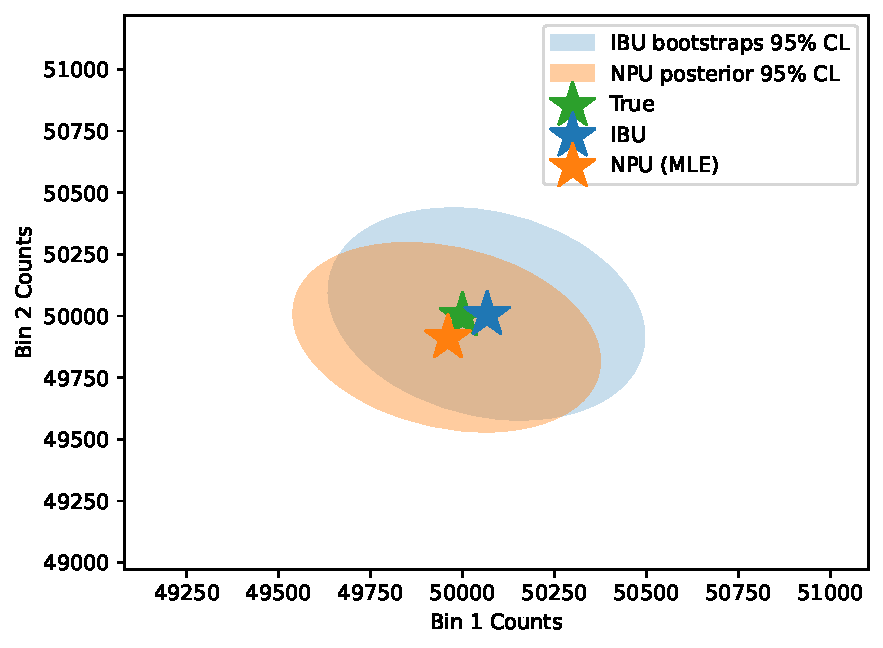
\includegraphics[width=0.485\textwidth]{figures/chapter-04/2bin_95CL.pdf}\label{fig:2bin:a}}
    \subfloat[2 bin example with degenerate response]{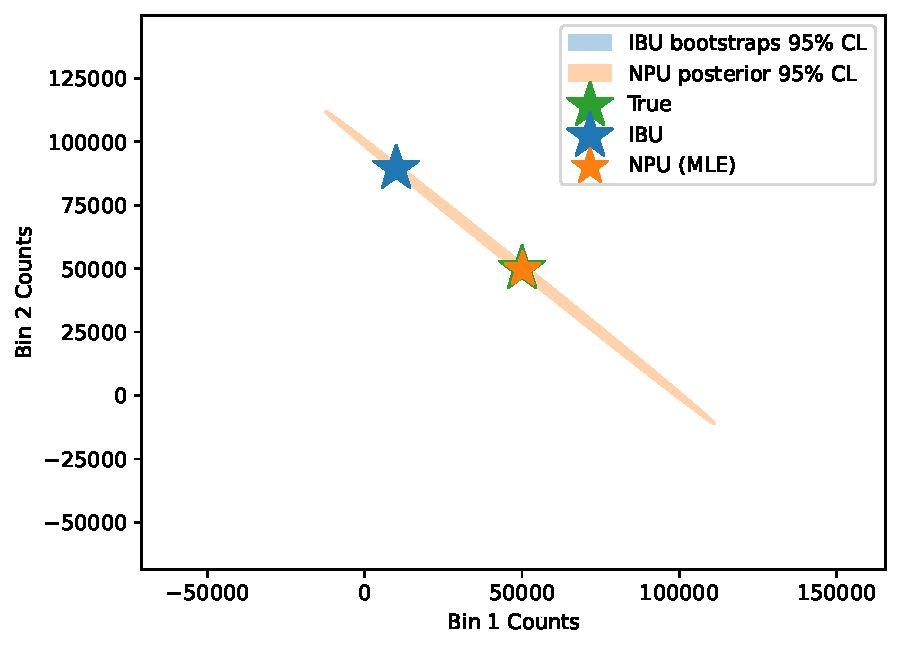
\includegraphics[width=0.49\textwidth]{figures/chapter-04/2bin_degenerateResp.pdf}\label{fig:2bin:b}}
    \caption[2 bin example]{Comparison between NPU and IBU using a two bin example.
    %
    The MLE estimate of NPU is shown with an orange star, the IBU prediction with a blue star, and the true value with a green star.
    %
    The orange and blue shaded regions represent the 95\% credible intervals of NPU and IBU, respectively.
    %
    \textbf{(a)} Non degenerate, nearly diagonal response matrix $(\rho = 0)$: 
    Both IBU and NPU yield unfolded distributions that agree well with the truth.
    %
    \textbf{(b)} Degenerate response $(R_{i\alpha} = R_{i\beta})$: 
    IBU relies solely on the prior, while NPU produces a full posterior with credible intervals that properly account for uncertainty in unconstrained regions.
    The NPU maximum likelihood estimate closely aligns with the true distribution, and the NPU posterior is compatible with the statistical uncertainty evaluated by IBU using bootstraps.\protect{\footnotemark}
    }
    \label{fig:2bin}
\end{figure}
\footnotetext{Figure created by Jingjing Pan.}

        This example highlights a fundamental advantage of NPU and other Bayesian methods;
        %
        they naturally capture uncertainty in unconstrained regions of phase space, while traditional methods like IBU can dramatically underestimate uncertainties when degeneracies are present.
\subsection{Gaussian example.}
    The second test employs a Gaussian distribution with known truth, allowing one to systematically evaluate NPU's performance with varying levels of detector smearing. 
    \subsubsection{Experimental setup}
Generate two from identical one dimensional Gaussian distributions with mean $\mu = 0$ and standard deviation $\sigma = 1$,
a generation dataset ({Gen.}) with $\num{d6}$ events for training, and a truth dataset ({Truth}) with $\num{d5}$ events for validation.

To simulate detector effects, apply Gaussian smearing with parameter $\epsilon = 0.5$ to both particle level datasets.
%
This produces corresponding detector level distributions, {Sim.}, from Gen., and {Data}, from Truth), both with the same mean but with increased width $\sigma_\text{detector} = \sqrt{1^2 + 0.5^2} \approx 1.12$.
%
The response matrix $\mathbf{R}$ is estimated from (Gen., Sim.) pairs.
%
This response matrix is then used to unfold the observed Data, with results compared against the known Truth.
%
The experimental setup and resulting response matrix are shown in \cref{fig:gaus_init}.
\begin{figure}
    \centering
    \subfloat[Experimental setup]{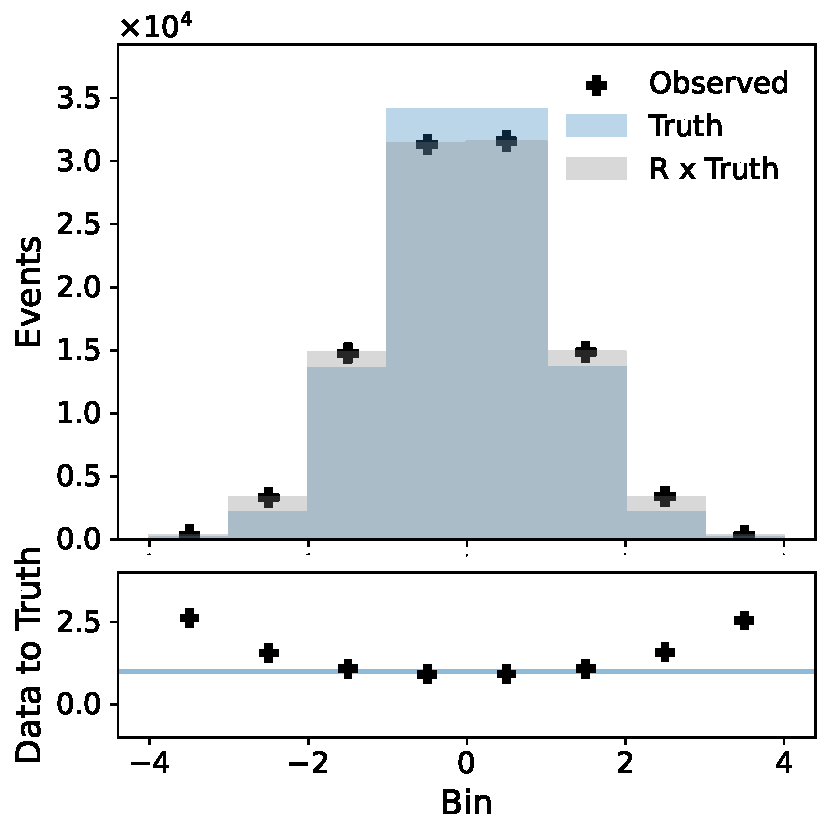
\includegraphics[width=0.45\textwidth]{figures/chapter-04/gaus_init.pdf}\label{fig:gaus_init:a}} 
    \subfloat[Response matrix]{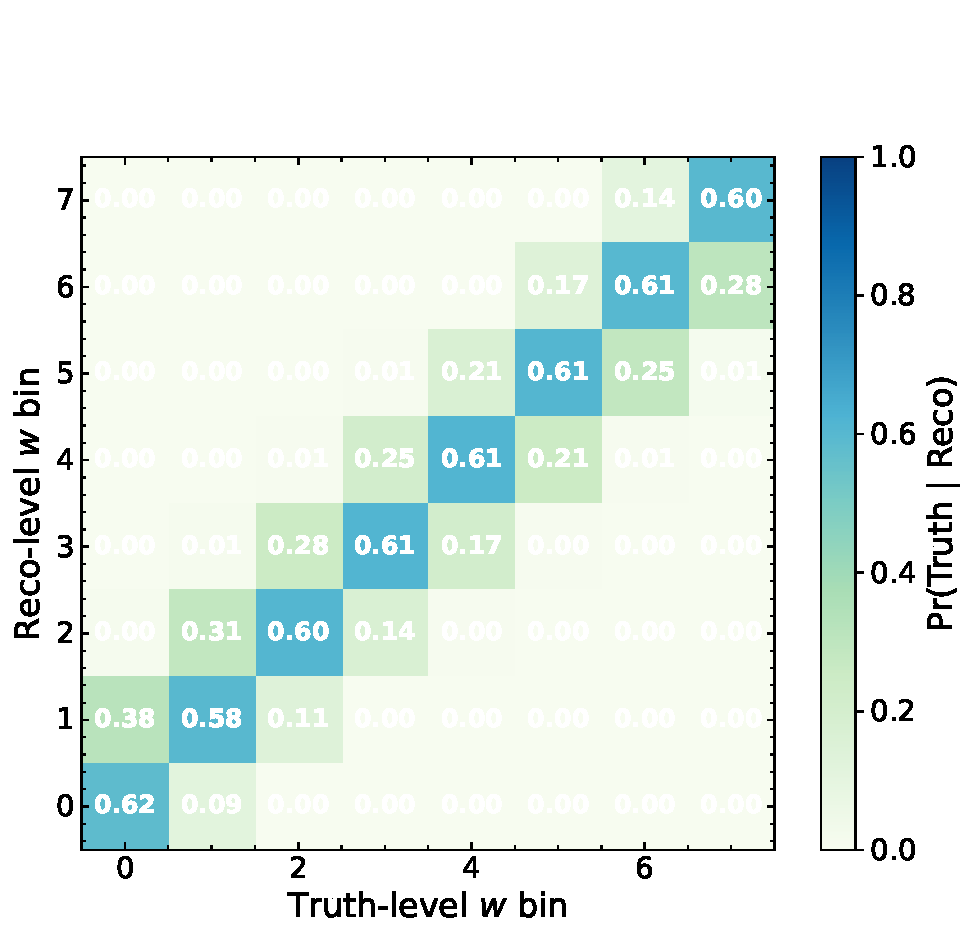
\includegraphics[width=0.535\textwidth]{figures/chapter-04/gaus_resp.pdf}\label{fig:gaus_init:b}} \\
    \caption[Gaussian example setup]{Gaussian unfolding example setup. 
    \textbf{(a)} The experimental design: Truth (blue) represents the target particle-level Gaussian distribution to be recovered, while Data (black crosses) shows the corresponding detector-level observations after Gaussian smearing. 
    %
    The goal of unfolding is to recover the Truth distribution from the observed Data.
    \textbf{(b)} The response matrix $\mathbf{R}$ constructed from Gen./Sim. pairs, which encodes the detector smearing transformation and serves as an input for the unfolding algorithms.
    %
    The matrix shows how probability mass spreads from each particle level bin (horizontal axis) to detector level bins (vertical axis).\footnotemark
    }
    \label{fig:gaus_init}
\end{figure}
\footnotetext{Figure created by Jingjing Pan.}
\subsubsection{Results and comparison}
    The unfolded distributions from NPU (Maximum Likelihood Estimate), IBU, and FBU all accurately recover the truth distribution, as shown in \cref{fig:gaus:a}.
    %
    Beyond point estimates, NPU provides a complete characterization of the uncertainty through its full posterior distribution, including bin-to-bin correlations visible in the corner plot in \cref{fig:gaus:b}.
    %
    This corner plot reveals the pairwise relationships between bins and demonstrates strong agreement between the posterior distributions from NPU and FBU, with both methods properly encompassing the true distribution.
\begin{figure}
\centering
\subfloat[Unfolded distributions]{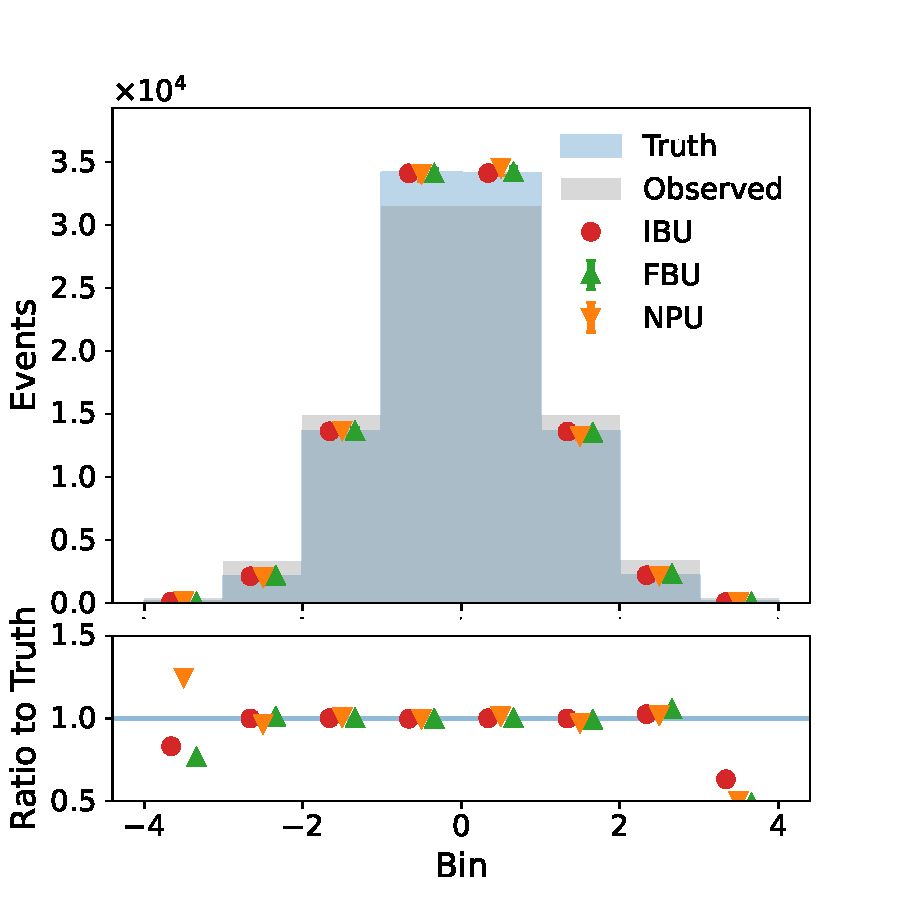
\includegraphics[width=0.48\textwidth]{figures/chapter-04/npu_gaussian_smearing_0.5.pdf}\label{fig:gaus:a}} 
\subfloat[Posterior correlations]{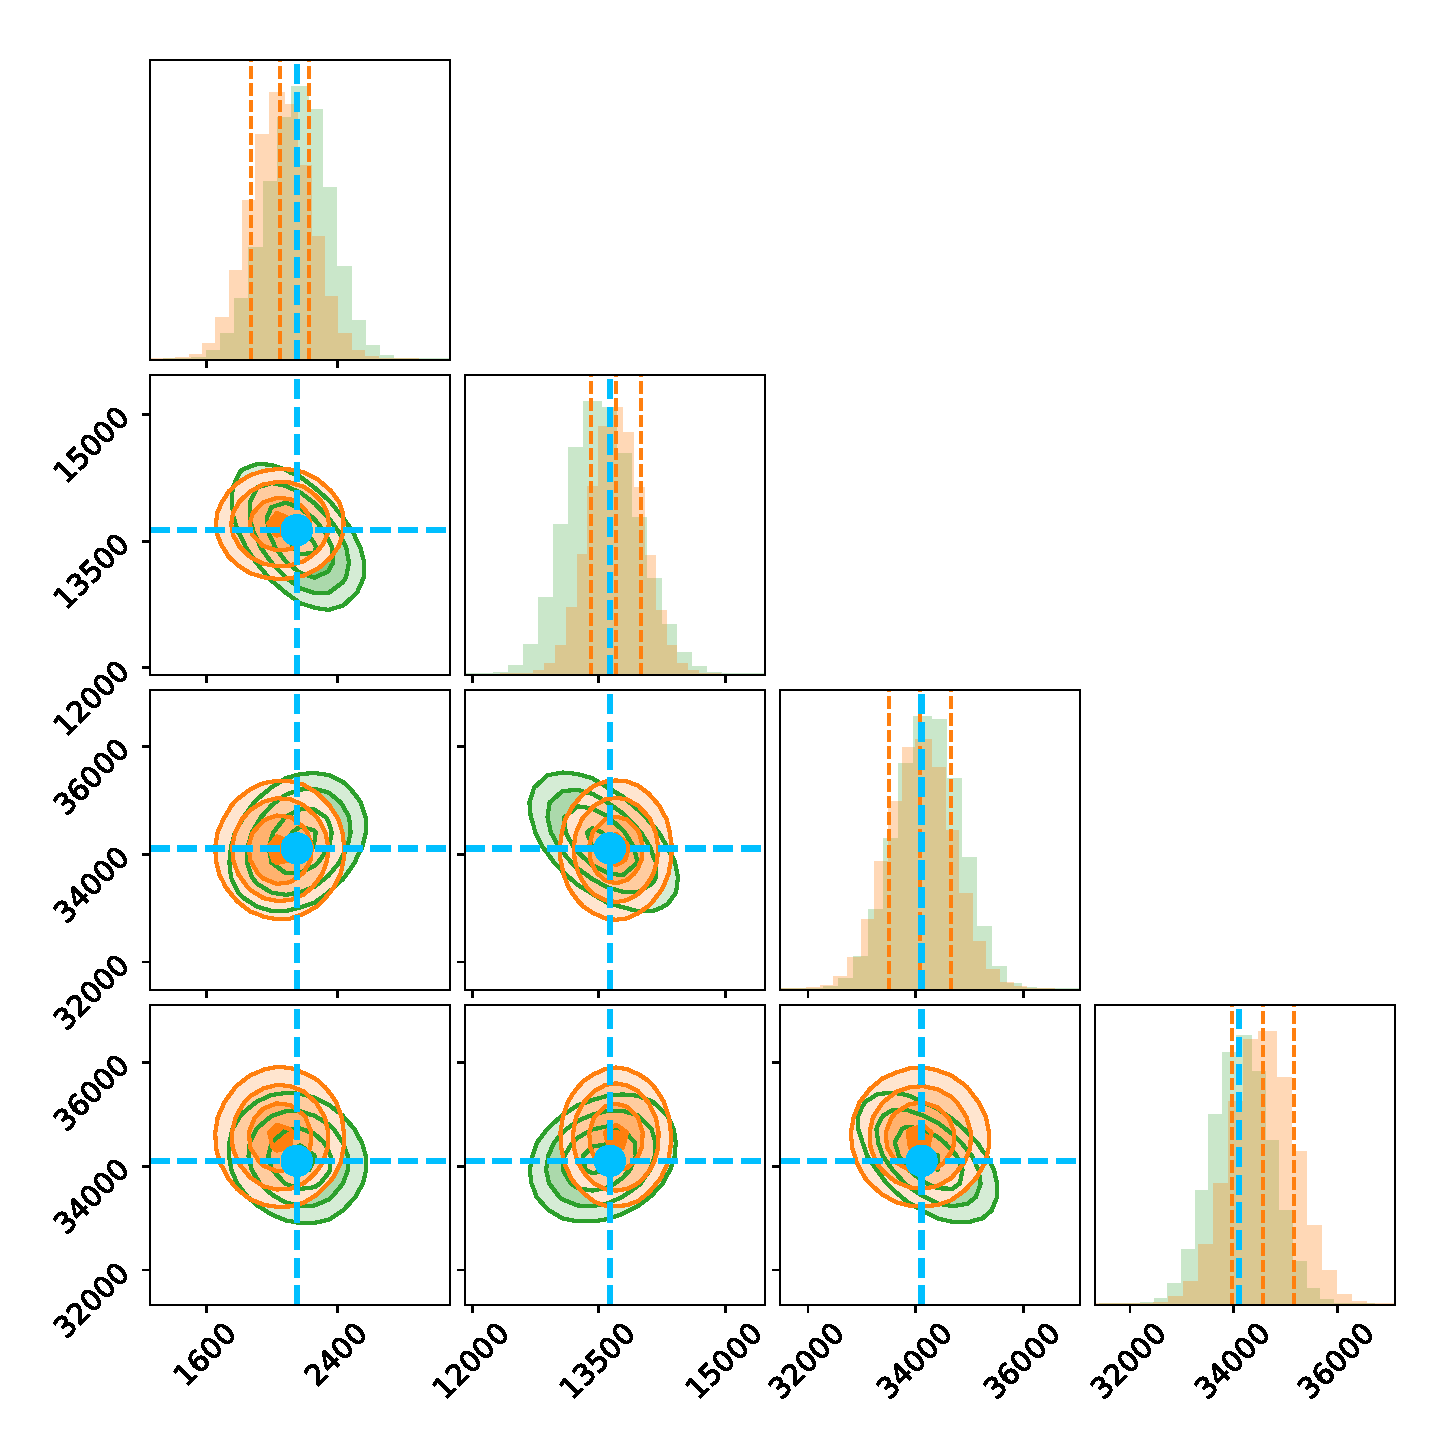
\includegraphics[width=0.48\textwidth]{figures/chapter-04/gaus_corner.pdf}\label{fig:gaus:b}} \\
\caption[Gaussian unfolding results and posterior analysis]{Gaussian unfolding results comparison.
\textbf{(a)} Unfolded distributions: NPU MLE (orange down triangles), IBU (red circles), and FBU (green up triangles) compared with truth (blue shaded region).
%
All methods successfully recover the true distribution.
%
\textbf{(b)} Corner plot showing pairwise posterior correlations between the four central bins from NPU (orange contours) and FBU (green contours, averaged over MCMC samples), with truth values marked in blue. 
Both methods show consistent posterior distributions that properly encompass the true values.
%
The green for FBU is averaged over many draws.\footnotemark
}
\label{fig:gaus}
\end{figure}
\footnotetext{Figure created by Jingjing Pan.}

    To rigorously assess the statistical calibration of NPU, evaluate pull distributions across 100 pseudo experiments.
    %
    For each bin $i$ in pseudo experiment $j$, compute the standardised residual:
    \[
        \text{Pull}_{ij} = \frac{\mu^{\text{method}}_{ij} - \nu_i}{\sigma^{\text{method}}_{ij}}
    \]
    where $\mu^{\text{method}}_{ij}$ and $\sigma^{\text{method}}_{ij}$ are the posterior mean and standard deviation for that bin, and $\nu_i$ is the true value.
    
    Recall from \cref{subsubsec:pull-distributions} that for properly calibrated uncertainty estimates, these pulls should follow a standard normal distribution with zero mean and unit variance.
    %
    As demonstrated in \cref{fig:pulls:a}, the pull distributions for both NPU and FBU with moderate smearing ($\epsilon = 0.5$) are indeed well centred at zero with unit width, confirming proper statistical calibration.
    %
    One can further tested the robustness of this calibration by varying the smearing parameter across $\epsilon \in [0.3, 0.6]$, finding that both methods maintain proper coverage throughout this range.
    %
    \cref{fig:pulls:b} 
\begin{table}
\centering
\caption[Computational cost comparison between FBU and NPU]{Computational cost comparison between FBU and NPU for repeated unfolding tasks. NPU's amortised inference approach provides significant speed-up despite the initial training overhead.}
\vspace{3mm}
\label{tab:timing}
\begin{tabular}{|l|c|c|c|}
\hline
\textbf{Method} & \textbf{Setup cost} & \textbf{Per run} & \textbf{Total (100 runs)} \\
\hline
FBU (10k MCMC draws) & -- & 40 sec & $\sim$67 min \\
NPU (amortised) & 280 sec & $\sim$2 sec & $\sim$5 min \\
\hline
\textbf{Speed-up} & \multicolumn{3}{c|}{\textbf{13$\times$ faster}} \\
\hline
\end{tabular}
\end{table}
\begin{figure}
\centering
\subfloat[Pull distributions for $\epsilon = 0.5$]{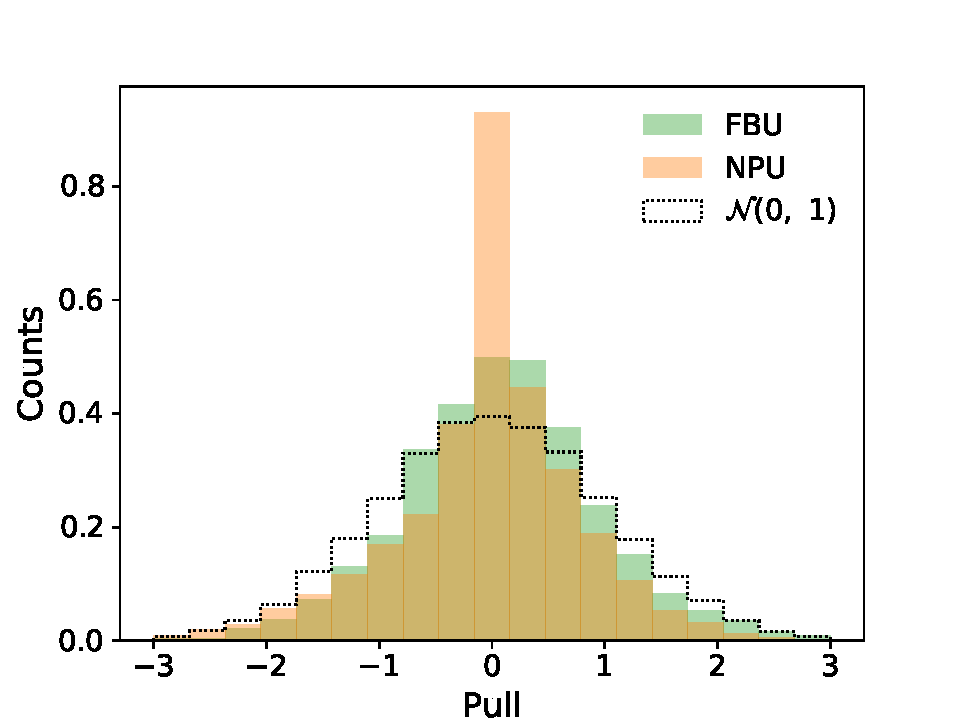
\includegraphics[width=0.48\textwidth]{figures/chapter-04/pulls_smear_0.5_N_100000.pdf}\label{fig:pulls:a}} 
\subfloat[Calibration across smearing parameters]{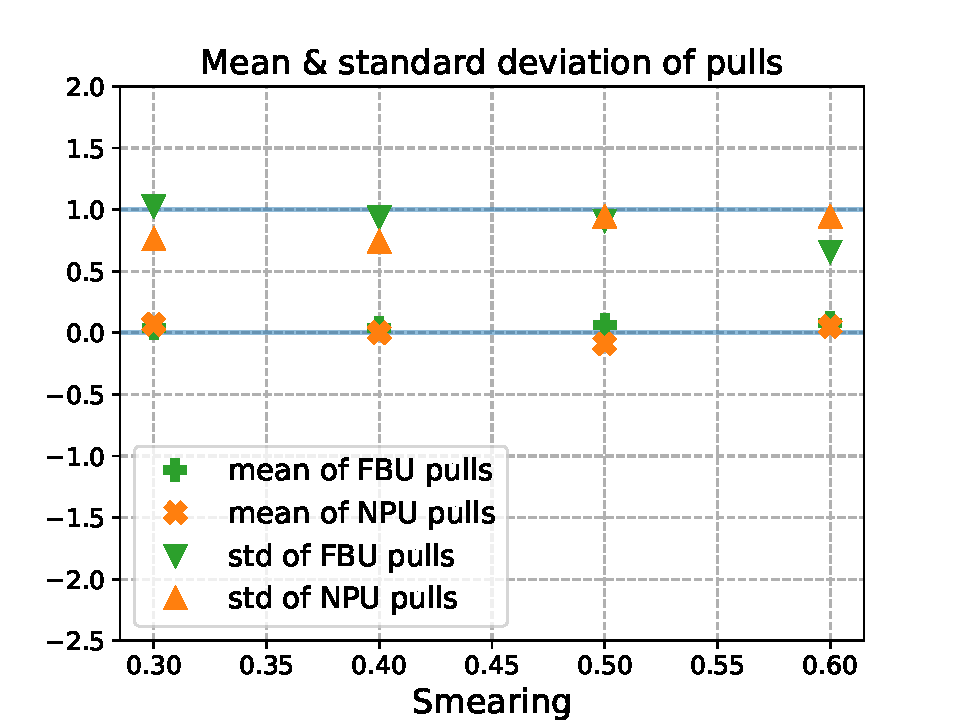
\includegraphics[width=0.48\textwidth]{figures/chapter-04/pulls_mean_std.pdf}\label{fig:pulls:b}} \\
\caption[Statistical calibration analysis for NPU and FBU]{Statistical calibration analysis from 100 pseudo-experiments.
\textbf{(a)} Pull distributions for NPU (orange) and FBU (green) with moderate smearing ($\epsilon = 0.5$), compared against the ideal $\mathcal{N}(0,1)$ reference (black line). 
Both methods show proper calibration with pulls centred at zero and unit variance.
\textbf{(b)} Pull distribution statistics as functions of smearing parameter $\epsilon \in [0.3, 0.6]$. 
The mean and standard deviation remain consistent with the ideal values ($\mu = 0$, $\sigma = 1$) across the range, confirming robust uncertainty quantification for both methods.\footnotemark
}
\label{fig:pulls}
\end{figure}
\footnotetext{Figure created by Jingjing Pan.}

This highlights an important practical advantage of NPU is its computational efficiency for repeated unfolding tasks.
%
In the benchmark with 100 pseudo experiments, FBU using \(\num{10,000}\) MCMC draws requires approximately \(\siqty{40}{\s}\) per experiment, totalling about \(\siqty{67}{\minute}\).
%
NPU requires about \(\siqty{280}{\s}\) for initial training but processes new datasets in just seconds each, yielding a total time of about \(\siqty{5}{\minute}\) for all \(\num{100}\) experiments.
%
This \(\numproduct{13x\,}\) speed-up stems from NPU's amortised inference approach, which eliminates repeated MCMC sampling for new datasets.
%
\cref{tab:timing} summarises the computational cost of NPU and FBU for 100 runs.

\subsection{Particle physics example.}
\begin{figure}
\centering
\subfloat[Jet width $\omega$]{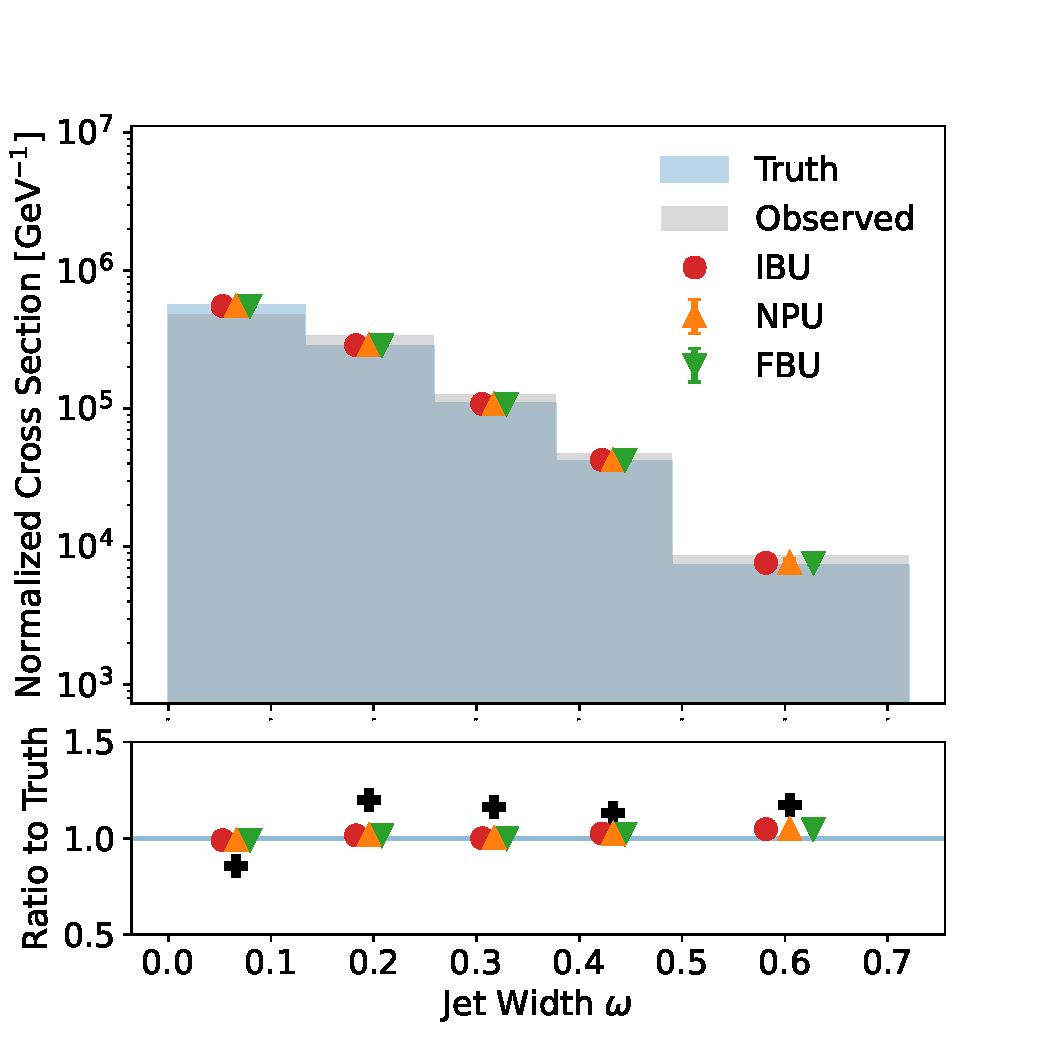
\includegraphics[width=0.46\textwidth]{figures/chapter-04/npu_width_logy.pdf}\label{fig:phys_width}} 
\subfloat[Groomed momentum fraction $z_g$]{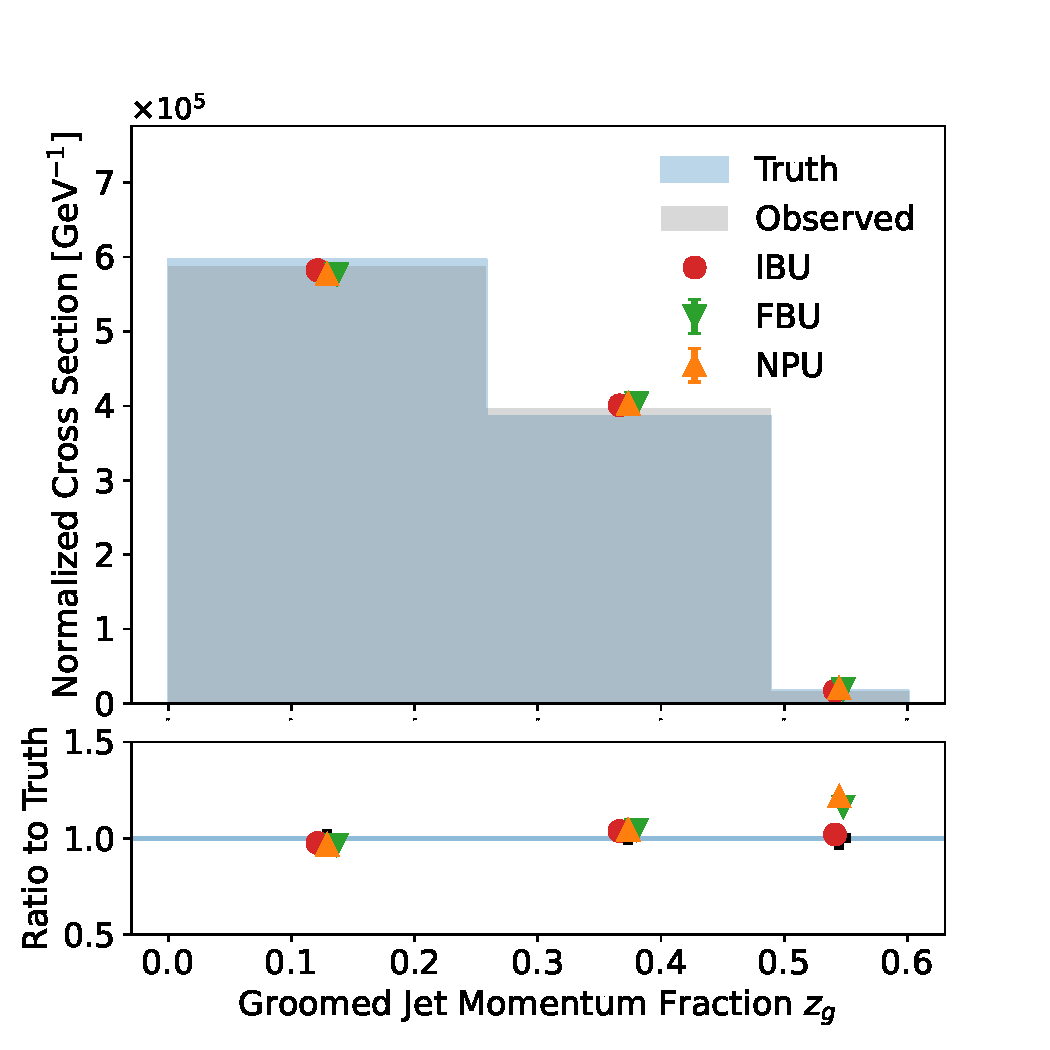
\includegraphics[width=0.46\textwidth]{figures/chapter-04/npu_zgs.pdf}\label{fig:phys_zg}} \\
\subfloat[$N$-subjettiness ratio $\tau_{21}^{\beta=1}$]{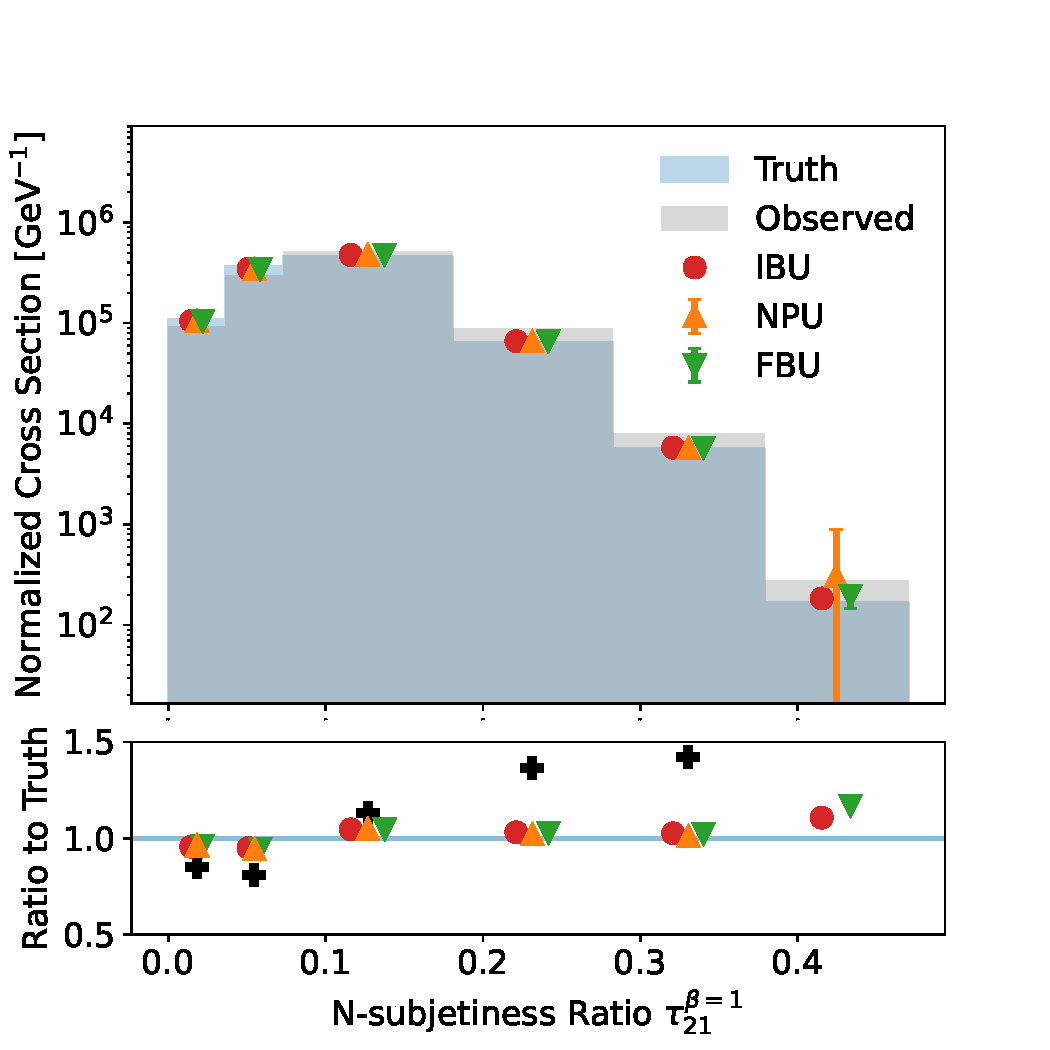
\includegraphics[width=0.46\textwidth]{figures/chapter-04/npu_tau2s_logy.pdf}\label{fig:phys_tau21}} 
\subfloat[Constituent multiplicity $M$]{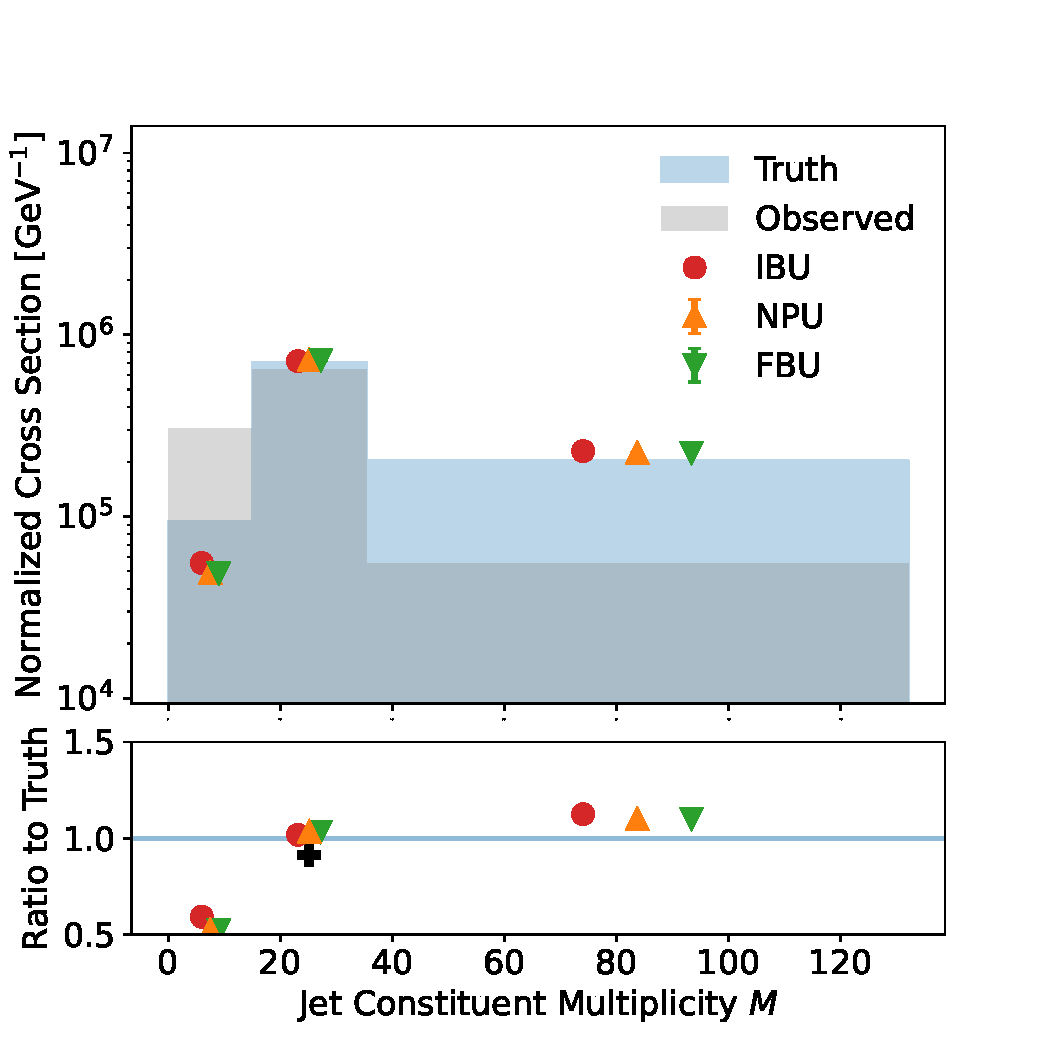
\includegraphics[width=0.46\textwidth]{figures/chapter-04/npu_mult_logy.pdf}\label{fig:phys_mult}} 
\caption[Jet substructure unfolding results using NPU, FBU, and IBU]{Unfolding results for jet substructure observables comparing NPU, FBU, and IBU methods.
The response matrix is constructed using \textsc{Pythia} 8.243 (Tune 21) simulation, while \textsc{Herwig} 7.1.5 provides both the observed data and particle level truth for validation.
%
Truth distributions are shown as blue shaded regions, with unfolded results from NPU (MLE as orange points), FBU (green points), and IBU (red points).
%
Error bars represent posterior standard deviations from the respective methods.
%
NPU successfully recovers the particle level truth distributions across all observables.\footnotemark
}
\label{fig:substructure}
\end{figure}
\footnotetext{Figure created by Jingjing Pan.}

    The final evaluation demonstrates NPU's application to a realistic hig -energy physics scenario, focusing on jet substructure measurements at the Large Hadron Collider (LHC).
    \subsubsection{Dataset and Observables}
        The dataset comprises simulated proton--proton collisions at $\sqrt{s} = 14$ TeV, following the setup in~\cite{andreassen_omnifold_2020}.
        %
        Two simulation generators are employed,
        \begin{itemize}
            \item \textsc{Herwig 7.1.5}~\cite{Bellm2017HerwigNote} serves as the data and truth distributions
            \item \textsc{Pythia 8.243} with Tune 21~\cite{bierlich_comprehensive_2022} is used to construct the response matrices.
        \end{itemize}
        
        Detector effects are emulated using \textsc{Delphes 3.4.2}~\cite{DeFavereau2014DELPHESExperiment}, a fast simulation of the CMS detector with particle flow reconstruction.
        %
        Jets are clustered using the anti$-k_T$ algorithm~\cite{Cacciari2008TheAlgorithm} with radius parameter $R = 0.4$, as implemented in \textsc{FastJet 3.3.2}~\cite{Cacciari2012FastJetManual}.
        %
        To minimize acceptance effects, this analysis includes only the leading jets in events containing a \(Z\) boson with transverse momentum \(p_T^Z > \siqty{200}{\GeV}\).
        %
        After selection, approximately \(\num{1.6d6}\) events from each simulation are retained.

        We focus on four key jet substructure observables that are widely used in LHC analyses.
        \begin{enumerate}
            \item Jet width (\(w\)): the transverse momentum weighted first radial moment of radiation within a jet,
            \item Jet constituent multiplicity ($M$): the number of constituents in a jet,
            \item \(N-\)subjettiness ratio ($\tau_{21} = \tau_2^{\beta=1}/\tau_1^{\beta=1}$): a measure of the compatibility of a jet with a two--prong substructure hypothesis relative to a one--prong hypothesis~\cite{Thaler2011IdentifyingN-subjettiness, Thaler2012MaximizingN-subjettiness, DevNairDevelopmentData}
            \item Groomed momentum fraction ($z_g$): the momentum sharing between sub--jets after soft drop grooming~\cite{Larkoski2014SoftDrop, Dasgupta2013TowardsSubstructure}
        \end{enumerate}
        These observables span a diverse range of physical characteristics and detector sensitivities, providing a comprehensive test of NPU's capabilities.
    \subsubsection{Results}
        \cref{fig:substructure} presents the unfolded distributions for each observable, comparing results from NPU, FBU, and IBU against the known truth.
        %
        For the FBU implementation in this more complex scenario, one needs to increase the number of MCMC steps ten fold compared to the Gaussian example, using \(\num{100000}\) tuning steps and \(\num{500000}\) draws.
        
        For all the observables, NPU accurately recovers the truth, with uncertainty bands that properly account for statistical uncertainties.
        %
        The results demonstrate a few different characteristics of NPU.
        %
        First, NPU effectively handles the complex detector effects present in realistic LHC simulations.
        %
        Second, the method exhibits robustness against simulation modeling differences: the response matrix is constructed using \textsc{Pythia} events, while the ``nature'' distribution NPU was expected to unfold was derived from \textsc{Herwig}, representing different underlying physics models and parton shower algorithms.
        %
        Finally, full posterior information enables rigorous uncertainty quantification across the entire distribution.
        %
        The corner plots for these distributions \cref{fig:phys-corner} reveal the complex correlation structure between bins, information that is typically unavailable with traditional unfolding methods unless explicitly computed via bootstrapping or similar approaches.

        These results highlight NPU's value for practical cross section measurements at HEP experiments, where detector effects are complex and true distributions may differ significantly from simulation.
        %
        In a complete experimental analysis, uncertainties in the response matrix itself could be incorporated either by repeating the unfolding procedure with systematically varied response matrices or by including these systematic uncertainties directly in the likelihood formulation.

\begin{figure}
\centering
\subfloat[Jet width $\omega$]{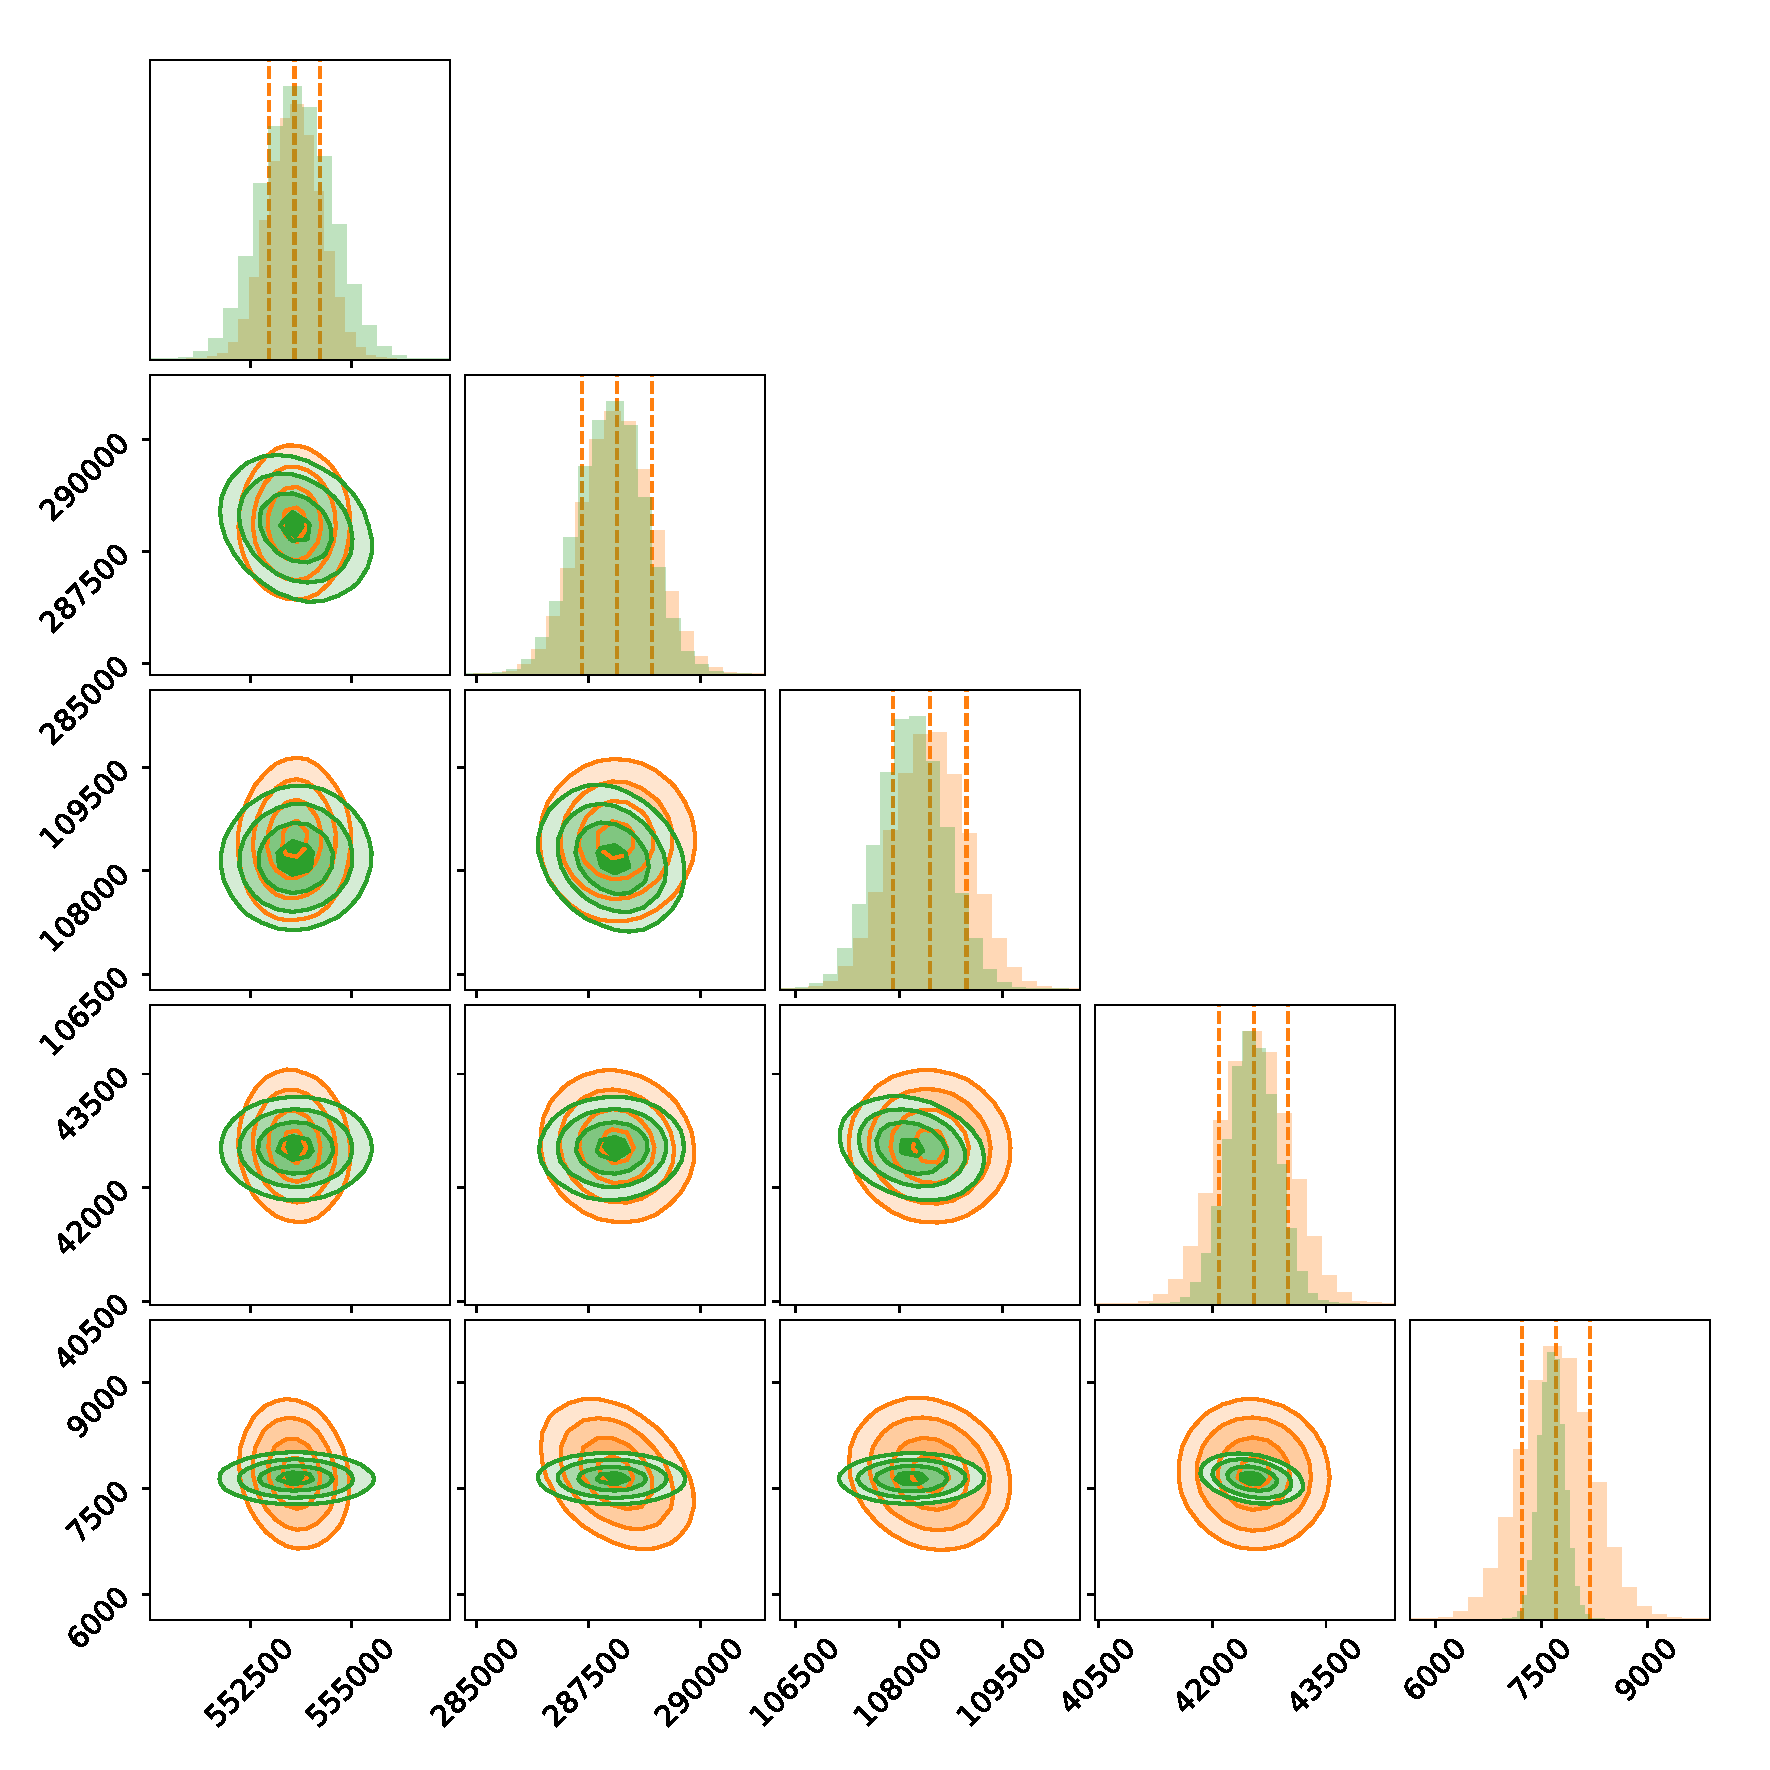
\includegraphics[width=0.45\textwidth]{figures/chapter-04/corner_both_width.pdf}\label{fig:corner_width}} 
\subfloat[Groomed momentum fraction $z_g$]{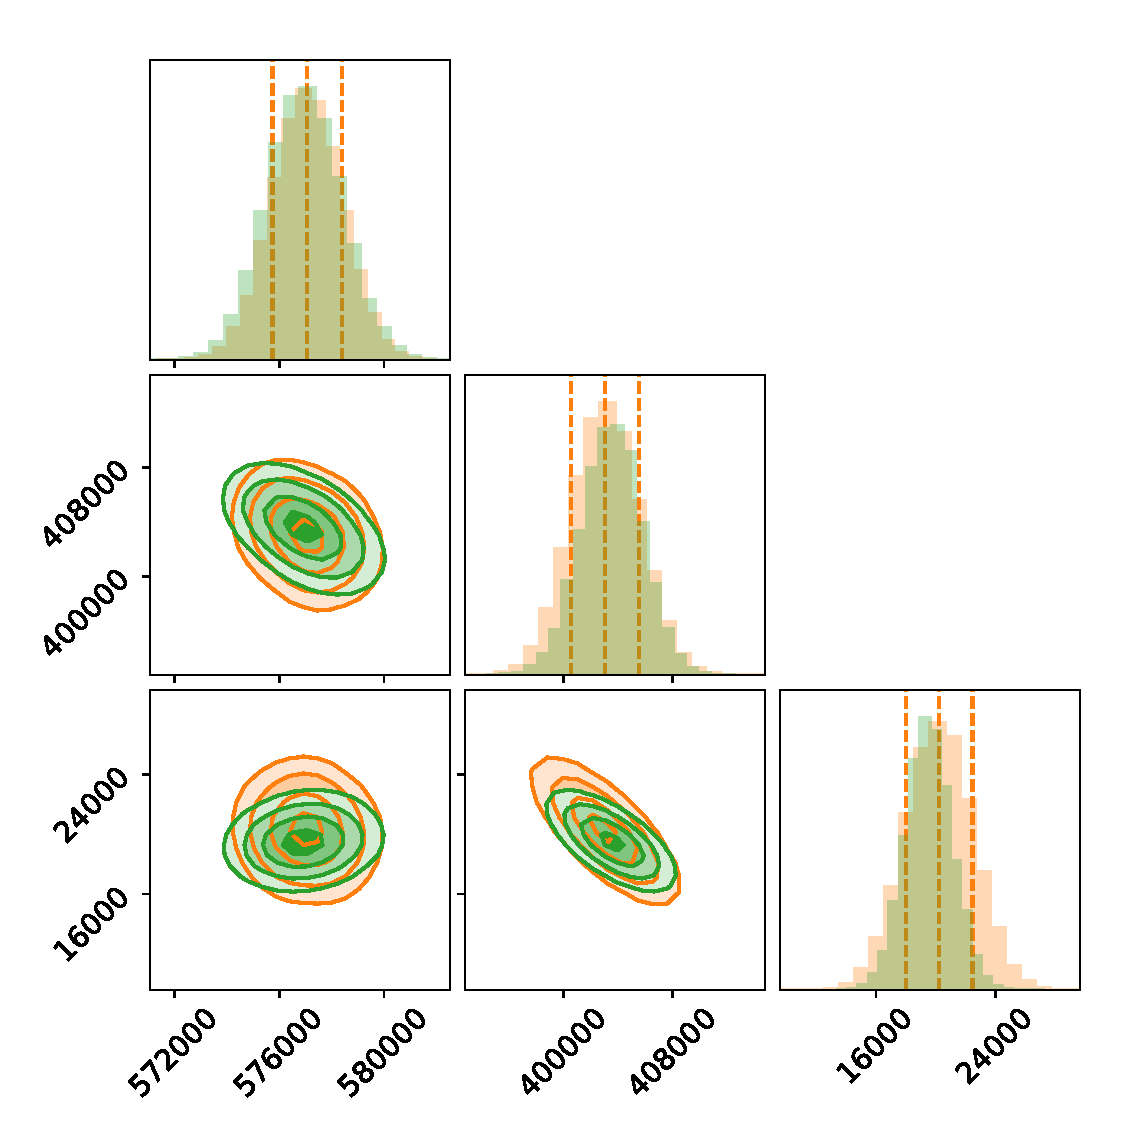
\includegraphics[width=0.45\textwidth]{figures/chapter-04/corner_both_zgs.pdf}\label{fig:corner_zg}}\\
\subfloat[Constituent multiplicity $M$]{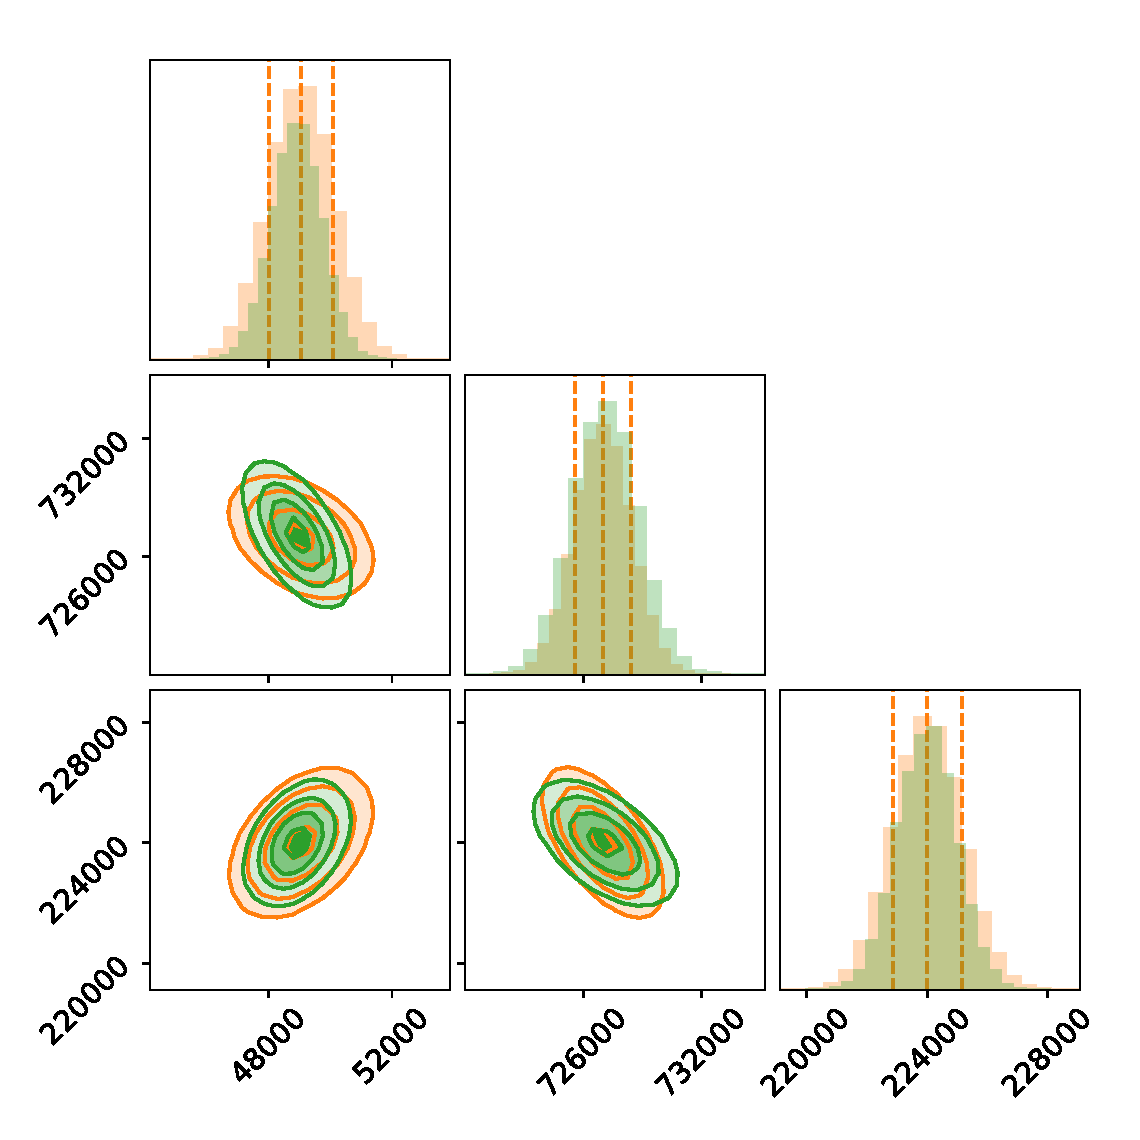
\includegraphics[width=0.45\textwidth]{figures/chapter-04/corner_both_mult.pdf}\label{fig:corner_mult}}
\subfloat[$N$-subjettiness ratio $\tau_{21}^{\beta=1}$]{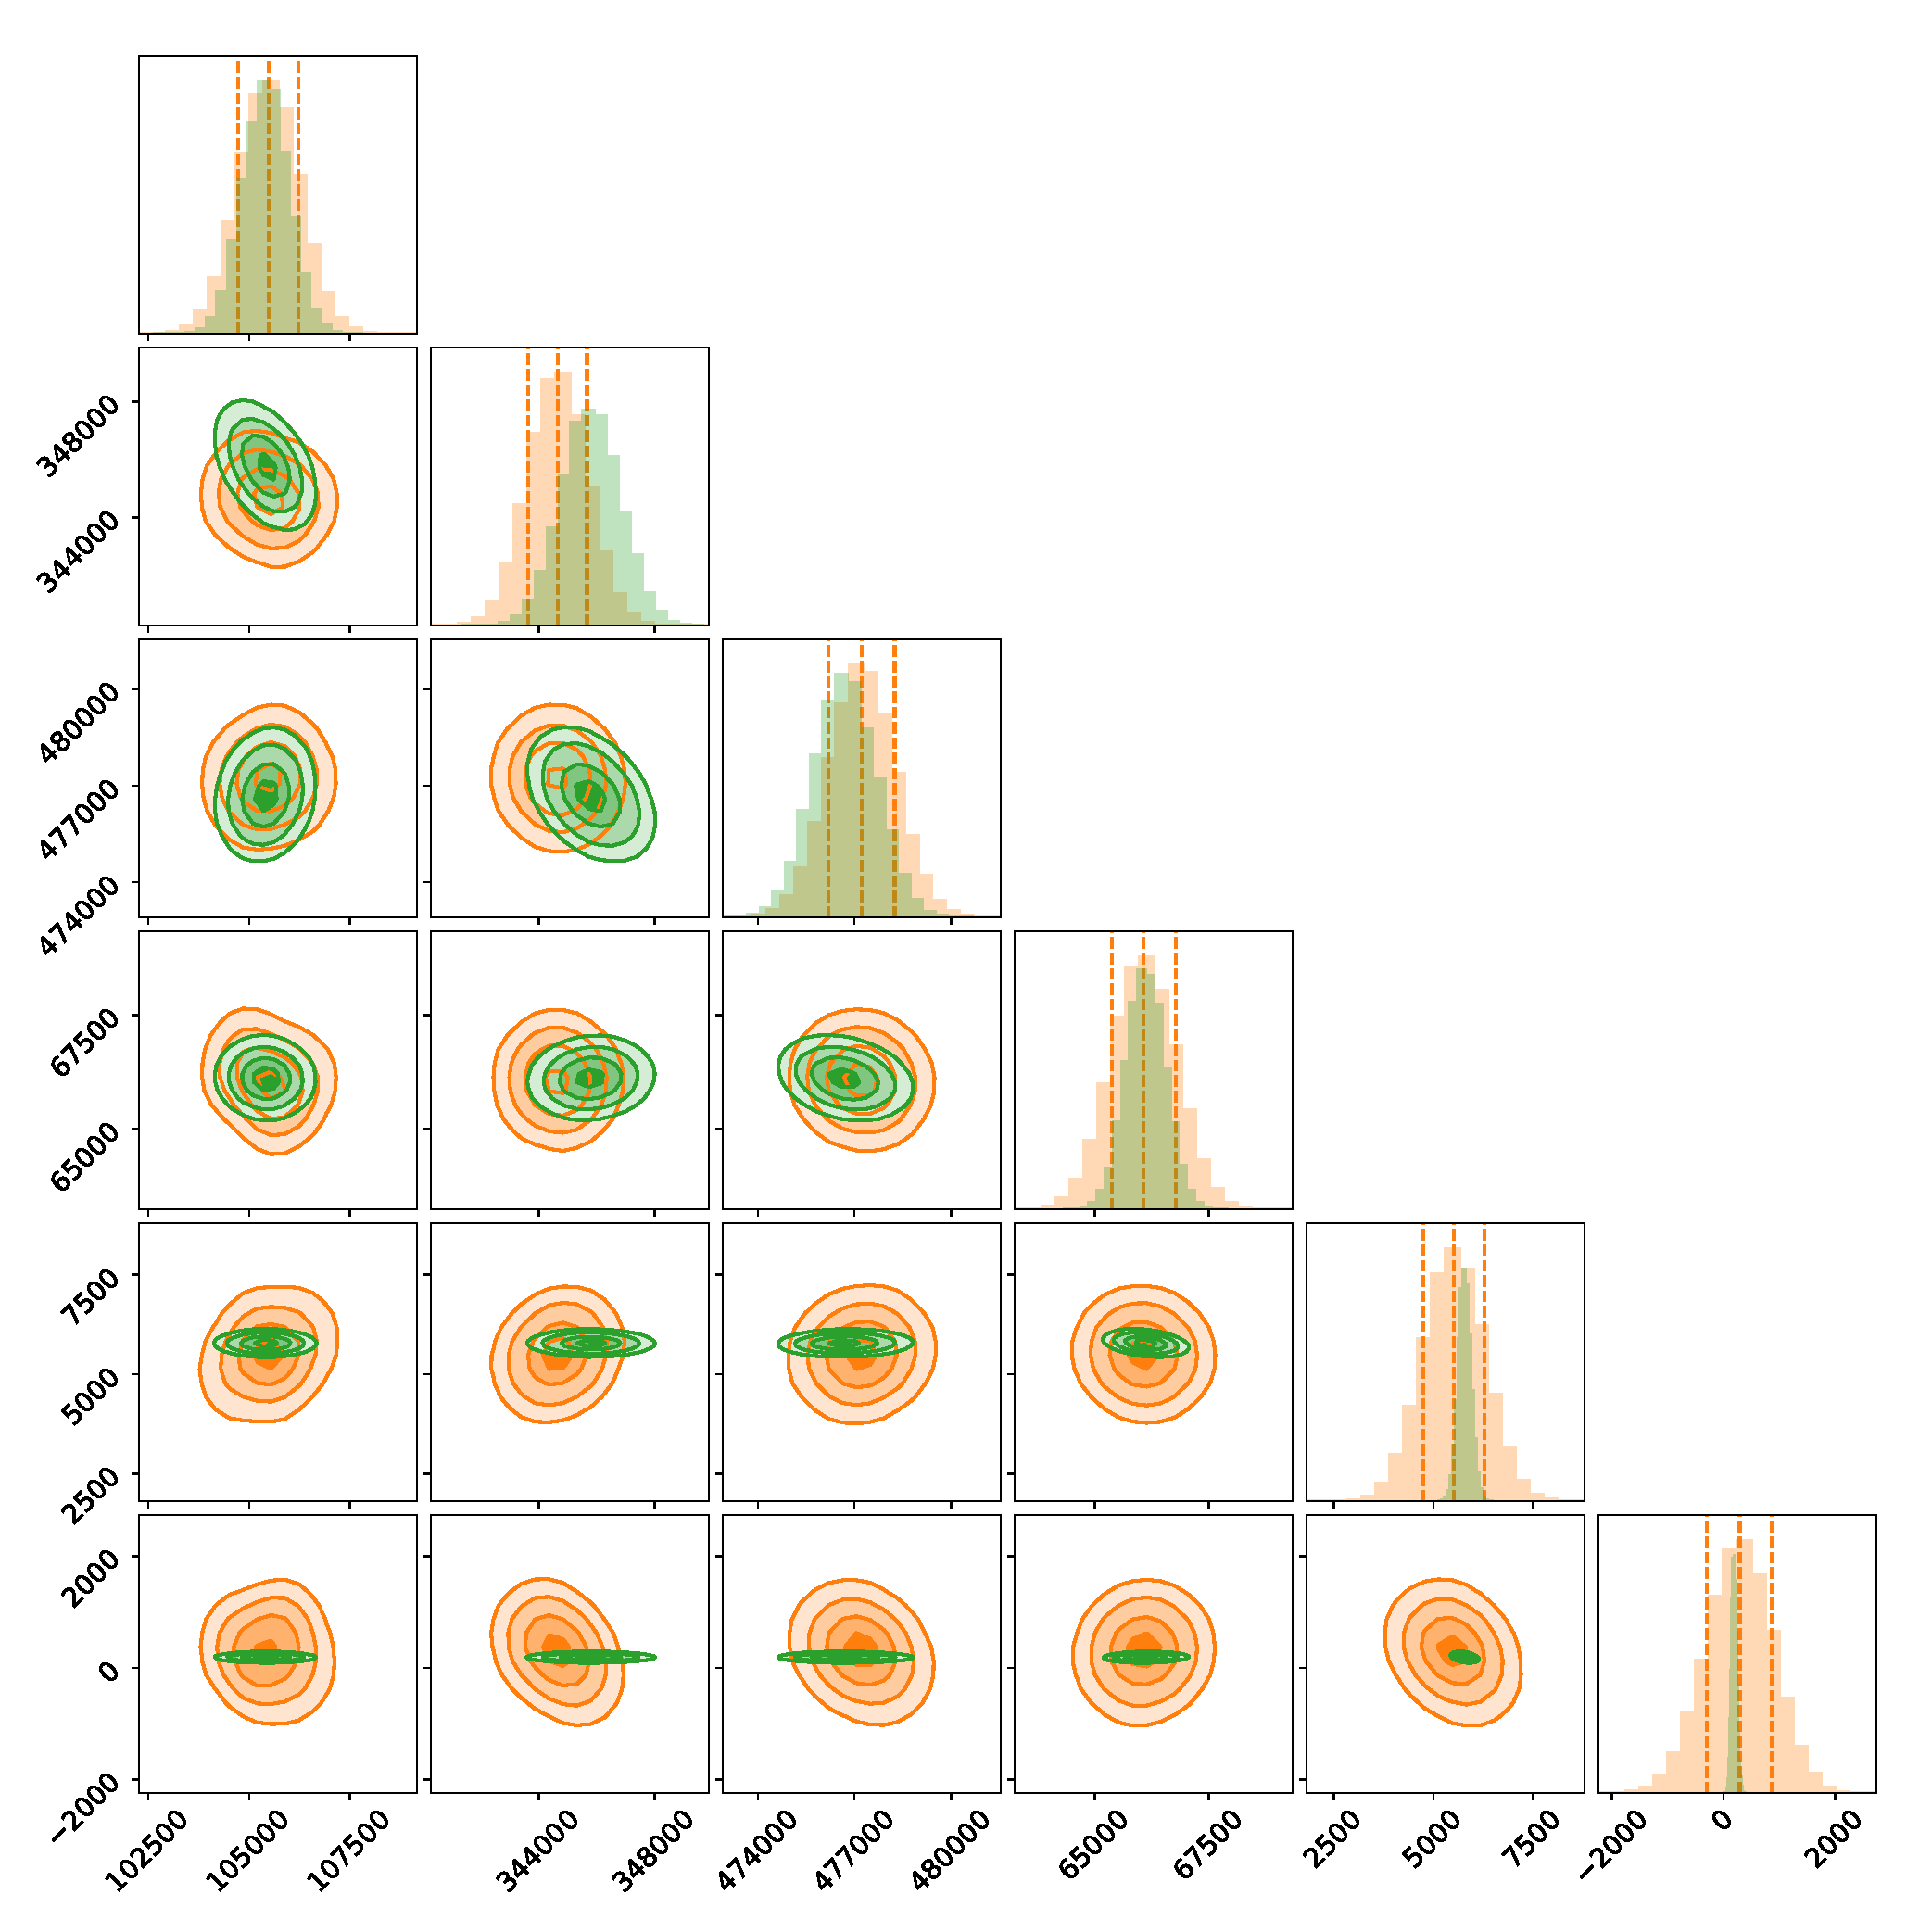
\includegraphics[width=0.45\textwidth]{figures/chapter-04/corner_both_tau2s.pdf}\label{fig:corner_tau21}}
\caption[Corner plots for jet substructure observables]{Corner plots showing posterior correlations for jet substructure observables.
Each panel displays pairwise correlations between bins for one observable, comparing NPU (orange contours) and FBU (green contours, averaged over MCMC samples) posteriors, with truth values marked in blue.
The plots reveal complex bin to bin correlation structures that are typically unavailable from traditional unfolding methods.
Strong agreement between NPU and FBU posteriors confirms the reliability of both approaches, while the encompassing of truth values validates proper uncertainty quantification.
These correlations provide crucial information for propagating uncertainties in downstream physics analyses.\footnotemark
}
\label{fig:phys-corner}
\end{figure}        
\footnotetext{Figure created by Jingjing Pan.}
\subsection{Summary of Numerical Results}
    These numerical studies demonstrate that NPU provides appropriate uncertainty quantification in degenerate scenarios where traditional methods fail, while maintaining proper statistical coverage across varying degrees of detector smearing.
    %
    NPU efficiently processes multiple datasets through amortized inference, and accurately recovers truth distributions in both targeted degenerate toy examples and realistic high energy physics scenarios.
    %
    The method combines the Bayesian foundations of FBU with several architectural and computational advantages.
    %
    The normalising flow architecture can represent a wide range of posterior distributions, including multimodal, asymmetric, and strongly correlated distributions that may be challenging for traditional MCMC methods.
    %
    By providing differentiable access to the posterior density, NPU enables gradient--based optimization for finding maximum likelihood estimates or other derived quantities.

    While FBU requires MCMC sampling for each new measurement, NPU's amortised inference approach front loads computational cost into the training phase.
    %
    Once trained, inference with NPU requires only forward passes through the neural network, making it particularly valuable for analysing large datasets, performing multiple analyses with different systematic variations, bootstrapping for uncertainty estimation, and studies requiring many unfolding runs
    %
    NPU also scales more favourably to high dimensional problems compared to MCMC based methods, which often suffer from the curse of dimensionality and mixing problems in complex posterior landscapes.
    
    However, several limitations should be kept in mind.
    %
    The flexibility of normalising flows comes with increased model complexity, requiring careful architecture design and hyperparameter tuning.
    %
    While less explicit than in traditional methods, NPU's results still depend on the distribution of the generated data, which implicitly defines a prior over the particle level histograms.
    %
    Also, as with any Bayesian method, it is important to validate that the posterior credible intervals have the correct frequentist coverage properties for critical analyses.
    
    Despite these considerations, NPU represents a significant advancement in unfolding methodology, combining the statistical rigour of Bayesian inference with the flexibility and computational efficiency of modern deep learning approaches making it a promising tool for cross section measurements in high energy physics.

\section{Beyond binning: the path forward}
    The Neural Posterior Unfolding method presented in this chapter represents a significant advancement in binned unfolding approaches.
    %
    By incorporating normalising flows for posterior estimation, NPU addresses several limitations of traditional methods while maintaining the established binning paradigm that has served particle physics for decades.
    %
    However, binning itself introduces fundamental constraints that motivate the development of alternative, unbinned methodologies.

    Binning inherently discards information about the precise location of events within each bin, reducing statistical precision.
    %
    The mantra ``The choice of binning is subjective and can introduce biases in the unfolded results'' is oft expressed in statistical treatments of the unfolding problem~\cite{cowan_survey_2002, cowan_statistics_2021, CowanStatisticalRehovot, Cowan2011AsymptoticPhysics,Tang2017DataMethod, hocker_svd_1996, Gagunashvili2024DataOptimization, CranmerPracticalLHC, StatisticalPhysics, Bohm2025IntroductionPhysicists, gardi_statistics_2015, Adam-Bourdarios2015TheChallenge, cowan_topics_2010}.
    %
    This discretisation is particularly problematic for observables with sharp features or resonances that may be obscured by bin boundaries.
    %
    The restrictions the curse of dimensionality imposes on binned methods' applicability to multivariate problems has already been discussed, 

    Binned methods require separate unfolding procedures for each differential distribution of interest.
    %
    This approach is inefficient when multiple observables derived from the same dataset need to be unfolded, as is common in comprehensive physics analyses.
    
    Recent years have seen the rapid development of unbinned unfolding methods powered by advances in deep learning.
    %
    These innovations have enabled significant progress towards solving the challenges posed by binned methods.
    %
    Although machine learning methods are typically a few orders of magnitude slower than traditional methods like IBU, modern ML techniques can leverage efficient data representations and parallelised computation for faster inference, reducing the gap particularly for high dimensional problems.

    The next chapters will explore some unbinned methods in detail, examining their theoretical foundations, practical implementations and performance characteristics on realistic physics examples.
    %
    These methods build upon the insights from binned approaches like NPU while overcoming the intrinsic limitations of binning to enable new capabilities for precision measurements in high energy physics.
    %
    As experimental datasets grow larger and theoretical predictions become more precise, unbinned methods will play an increasingly important role in extracting the full physics potential from experiments.
    %
    The transition from binned to unbinned unfolding represents not just a technical evolution but a paradigm shift in how we approach the measurement and interpretation of cross section measurements.
\chapter{Moment Unfolding: Direct Deconvolution of Distribution Moments}
\label{chap:moment-unfolding}
\section{Why Moments: Physics Context and QCD Calculations}
    Statistical moments of probability distributions serve as powerful tools in physics, providing a concise and theoretically meaningful way to characterise complex phenomena.
    %
    In the context of particle physics, and particularly in quantum chromodynamics (QCD), working at the level of moments rather than distributions offers significant advantages for both theoretical calculations and experimental measurements.
    %
    This section explores the fundamental importance of moments in physics, their theoretical foundations, and their specific applications in QCD.
    \subsection{The Theoretical Significance of Moments in Physics}
        Statistical moments represent a systematic way to characterize probability distributions, with each successive moment providing additional information about the shape and properties of the distribution.
        %
        The $k$-th moment of a probability density $p(z)$ is defined as
        \[
            \langle Z^k \rangle = \int_{-\infty}^{\infty} z^k p(z) dz
        \]
        While the complete probability distribution contains all available information, working with moment is often much more tractable.
        %
        In many physical theories, moments can be calculated analytically even when full distributions cannot.
        %
        Each moment has a direct physical interpretation--the first moment corresponds to the mean, the second moment to the variance, and higher moments characterize asymmetry (skewness) and peakedness (kurtosis).
        %
        Moments therefore provide much more concrete insight into the properties of an observable than distributions.
        
        In many physical theories, including QCD, there exist relatively simple evolution equations for how moments change as a function of energy scale.
        %
        If certain moments exhibit universal behaviour across different physical systems, this too reveals universality in the fundamental underlying principles.
        %
        For many physical systems, including those governed by QCD, moments provide a natural language for connecting theoretical predictions with experimental measurements, particularly when examining how observables scale with energy.
    \subsection{Moments in QCD Calculations}
        In quantum chromodynamics, moments play a particularly crucial role in understanding the scaling behaviour of parton distributions and fragmentation functions.
        %
        The DGLAP equations form the theoretical framework for parton distribution function evolution. 
        \subsubsection{DGLAP Evolution Equations}
            The Dokshitzer--Gribov--Lipatov--Altarelli--Parisi (DGLAP) evolution equations\kd{cite} govern how parton distribution functions evolve with energy scale.
            %
            While these equations are integro--differential equations in their most general form, they transform into ordinary differential equations when expressed in terms of moments, significantly simplifying their solution \kd{cite}.

            For a parton distribution function $f(x,Q^2)$, where $x$ is the momentum fraction and $Q^2$ is the energy scale, the $n-$th moment is defined as
            \[
                M_n(Q^2) = \int_0^1 x^{n-1}\;f(x,Q^2) \dd x.
            \]
            The DGLAP equations for these moments take the form
            \[
            \frac{\dd M_n(Q^2)}{\dd \ln Q^2} = \frac{\alpha_s(Q^2)}{2\pi}\; P_n\;M_n(Q^2).
            \]
            where $P_n$ are the moments of the splitting functions.
            %
            This formulation converts the complex integro--differential evolution equations into a set of simple ordinary differential equations, one for each moment independently.

        \subsubsection{Operator Product Expansion}
            The Operator Product Expansion (OPE) in QCD naturally expresses deep inelastic scattering structure functions in terms of moments \kd{cite}.
            %
            In this formalism, the moments of structure functions are related to matrix elements of local operators, which have clear physical interpretations and scaling properties.
            %
            For example, the moments of the structure function $F_2(x,Q^2)$ can be expressed as
            \[
                M_n(Q^2) = \int_0^1 x^{n-2}\;F_2(x,Q^2)\;\dd x = \sum_i C_n^i(Q^2) \;\langle O_n^i \rangle.
            \]
            where $C_n^i$ are Wilson coefficients calculable in perturbation theory, and $\langle O_n^i \rangle$ are matrix elements of local operators.
        \subsubsection{Event Shape Moments}
            Event shape observables, which characterize the geometrical properties of energy flow in collisions, are often studied through their moments.
            %
            Moments of event shapes like thrust, broadening, and jet mass distributions provide sensitive tests of perturbative QCD and allow precise extractions of the strong coupling constant $\alpha_s$ \kd{cite}.
            %
            The moments of these event shapes can be calculated as
            \[
                \langle e^n \rangle = \int_0^{e_{\text{max}}} e^n \;\frac{1}{\sigma}\; \frac{\dd\sigma}{\dd e}\; \dd e,
            \]
            where $e$ is the event shape variable, and $\frac{1}{\sigma} \frac{\dd\sigma}{\dd e}$ is its normalized differential cross section.
            %
            These moments can be predicted in perturbative QCD, typically expressed as power series in $\alpha_s$:
            \[
                \langle e^n \rangle = A_n \left(\frac{\alpha_s}{2\pi}\right) + B_n \left(\frac{\alpha_s}{2\pi}\right)^2 + \mathcal{O}(\alpha_s^3),
            \]
            plus non--perturbative corrections that scale as inverse powers of the centre--of--mass energy.
    \subsection{Experimental Significance of Moments in QCD}
        From an experimental perspective, moments offer several advantages that make them particularly valuable for QCD studies.

        Some of the most precise determinations of the strong coupling constant $\alpha_s$ come from measurements of moments.
        %
        For example, moments of event shapes measured at LEP have provided determinations of $\alpha_s$ with uncertainties at the few-percent level \kd{cite}.
        %
        Studies by AMY, TASSO, OPAL, DELPHI, L3, and ALEPH collaborations have all used moment--based analyses to extract $\alpha_s$ values that contribute significantly to the world average \kd{cite}.

        The scaling behavior of moments with energy provides a direct and robust window into the running of QCD couplings.
        %
        By measuring how moments of distributions change with energy scale, experiments can observe the logarithmic scaling violations that are a hallmark of asymptotic freedom in QCD \kd{cite}.

        Many theoretical QCD calculations are more readily available (and more precise) for moments than for full distributions.
        %
        For certain observables, perturbative calculations may exist to next--to--next--to--leading order (NNLO) or beyond for moments, while full distribution calculations may only be available at lower orders \kd{cite}.
        
        In practice, measuring moments directly can reduce certain experimental uncertainties, particularly those related to detector resolution and acceptance effects in regions of phase space with sparse statistics.

        Traditionally, there was no straightforward method to directly unfold moments.
        %
        Instead, moments were computed after first measuring and unfolding the full distribution.
        %
        This typically involved binning the data, unfolding the binned distribution, and then computing moments from the unfolded histogram.
        %
        The limitation of this approach though, is the binning itself, not the moments qua moments.
        
        The use of discrete bins introduces a bias in moment calculations.
        %
        For a variable $z$ binned into $n_{\text{bins}}$ with centers $z_{\text{bin},i}$ and counts $N_i$, the binned approximation of the $k-$th moment is
        \[
            \langle z^k \rangle_{\text{bin}} = \frac{1}{N} \sum_{i=1}^{n_{\text{bins}}} N_i z_{\text{bin},i}^k
        \]
        This approximation introduces a bias relative to the true moment, which grows with the order of the moment computed, and is particularly large in regions where the distribution varies rapidly within bins \kd{cite}.

        These limitations motivate the development of unbinned approaches that can directly unfold moments without first discretizing the data, which is precisely the focus of the Moment Unfolding method described in this chapter.
    \subsection{Applications in Jet Physics}
        In the context of jet physics specifically---a central arena for testing QCD---moments of jet substructure observables provide particularly powerful probes of QCD dynamics \kd{cite}>.
        %
        Several notable applications deserve special mention.
        
        The energy scale dependence of jet properties is best studied through their moments.
        %
        The moments of jet substructure observables such as jet mass, width, and multiplicity exhibit characteristic scaling with jet energy that can be predicted by perturbative QCD. For example, the first moment of the jet mass scales approximately as \kd{cite}>
        \[
            \langle m^2 \rangle \propto \alpha_s(p_T) \;p_T^2 \;\ln(R/R_0)
        \]
        where $p_T$ is the jet transverse momentum, $R$ is the jet radius, and $R_0$ is the reference scale.
        %
        Higher moments have different scaling behaviours, providing multiple handles on the underlying QCD dynamics.

        The moments of jet substructure variables are also used in the classification of jets.
        %
        This is because jet moments differ characteristically between quark--initiated and gluon--initiated jets, making them valuable for jet flavour tagging.
        %
        For instance, gluon jets typically have higher multiplicity and broader mass distributions than quark jets, reflected in the moments of these distributions \kd{cite}.
    
        Jet substructure moments also provide a window to study non--perturbative effects and hadronization.
        %
        The interplay between perturbative and non-perturbative effects in QCD is particularly evident in moments of jet observables.
        %
        Lower moments often capture the perturbative, large--angle radiation physics, while higher moments become increasingly sensitive to non--perturbative effects like hadronization \kd{cite}.
    
        In the context of Soft-Collinear Effective Theory (SCET), moments of jet substructure observables provide direct constraints on the parameters of the effective theory, offering a bridge between first--principles QCD and phenomenological models of jet formation \kd{cite}.

        \subsubsection{Moments in Physics Beyond the Standard Model}
            While moments are crucial for precision QCD studies, their utility extends to searches for BSM physics.
            %
            Certain moments of distributions can exhibit enhanced sensitivity to new physics scales.
            %
            For example, higher moments of mass distributions can be more sensitive to heavy particle contributions than the full distribution average \kd{cite}.
    
            Moments can therefore provide a model--independent way to parametrize deviations from Standard Model predictions, similar to the role of effective field theory coefficients.
            %
            By measuring a series of moments, experiments can place constraints on a wide class of possible new physics scenarios without committing to specific models \kd{cite}.
            %
            Hence, changes in the moment structure of distributions can serve as an early indicator of anomalous physics, even before the full nature of the anomaly is understood <kd{cite}>.

    \subsection{The Case for Direct Moment Unfolding}
        Given the theoretical significance of moments in QCD and their experimental advantages, there is a strong motivation for developing methods that can directly unfold moments from detector--level data without first unfolding the entire distribution.
        %
        Such methods would eliminate binning biases inherent in traditional approaches, while potentially improving precision and reducing computational cost by focusing directly on the quantities of interest.
        %
        They would enable moment measurements in higher--dimensional phase spaces where binned approaches become impractical to provide more direct comparisons with theoretical predictions that are formulated at the level of moments.

        The remainder of this chapter presents the Moment Unfolding method, a novel approach that addresses precisely this need by directly deconvolving moments of distributions using machine learning techniques inspired by the Boltzmann distribution and implemented through a GAN--like architecture.
        %
        This method offers a significant advance in precision moment measurements, enabling more stringent tests of QCD predictions and potentially uncovering subtle effects that might be obscured in traditional analyses.
\section{A GAN--like Method to Unfold Moments}
    The direct extraction of distribution moments without first reconstructing the entire distribution presents a unique challenge in unfolding methodology.
    %
    Traditional approaches typically reconstruct the full differential cross--section before computing moments, introducing unnecessary computational complexity.
    %
    The Moment Unfolding technique presented in this chapter takes an entirely different approach by directly targeting the moments themselves.

    The basic idea underlying Moment Unfolding is the connection between statistical moments and the Boltzmann distribution from statistical mechanics.
    %
    In thermodynamics, the Boltzmann distribution represents the probability distribution that maximizes entropy while satisfying certain constraints on average quantities (internal energy). 
    %
    This principle can be adapted for our unfolding problem, where we seek to find a reweighting of simulated events that accurately reproduces the moments of the true particle--level distribution.
    \subsection{Boltzmann inspired reweighting}
        The central mathematical construction of Moment Unfolding is a reweighting function inspired by the Boltzmann factor,
        \[
            \label{eq:moment-generator}
            g(z) = \frac{1}{P(\vb*{\beta})} \exp\left(-\sum_{a=1}^n \beta_a \; z^a\right)
        \]
        where $z$ is the particle--level observable whose moments we wish to unfold, $\beta_a$ are parameters to be determined (analogous to Lagrange multipliers in statistical mechanics), $P$ is a normalization factor similar to the partition function, and $n$ is the number of moments we aim to unfold simultaneously.

        This form is particularly powerful because it directly connects to the maximum entropy principle in statistical mechanics.
        %
        Just as the Boltzmann distribution maximizes entropy subject to constraints on average energy, this reweighting function maximizes the binary cross entropy loss between the discriminator's classification output between the reweighted distribution and the prior distribution while enforcing constraints on the moments.
        %
        When applied to a simulated particle--level distribution with probability density $q_{\text{Gen.}}(z)$, this reweighting function produces a modified distribution
        \[
            \widetilde{q}(z) = g(z) \cdot q_{\text{Gen.}}(z)
        \]
        The training objective then is to determine the optimal values of the parameters $\beta_a$ such that the moments of $\widetilde{q}(z)$ match those of the true underlying distribution \(p(z)\).
    \subsection{Adversarial Training Framework}
        Given the theoretical foundation provided by the Boltzmann form, we now need a practical method to determine the optimal parameters.
        %
        The task can very naturally be framed as a two--level optimization problem:
        \begin{enumerate}
            \item The parameters $\beta_a$ control the reweighting at the particle level
            \item The quality of the reweighting must be assessed at the detector level
        \end{enumerate}
        This task is highly non--trivial because the detector response function—which maps particle-level to detector--level observables—-is typically stochastic and known only implicitly through simulation.
    
        To address this, Moment Unfolding employs an adversarial training architecture inspired by Generative Adversarial Networks (GANs), but with significant modifications tailored to the unfolding problem.
        %
        Unlike traditional GANs that generate new samples, our ``generator" $g(z)$ reweights existing particle-level simulated events according to the Boltzmann form.
        %
        The discriminator is a neural network classifier $d(x)$ that attempts to distinguish between real detector--level data and the reweighted simulation at detector level.

        The system is then trained adversarially, with the generator attempting to fool the discriminator while the discriminator attempts to correctly classify events.
        %
        This setup is illustrated in Figure~\kd{fig:moment-unfolding-architecture}, showing the flow of information and the adversarial training process.
        %
        In this framework, the optimal parameters $\beta_a$ are those that make the reweighted detector--level simulation indistinguishable from the real detector--level data.
        %
        Once these parameters are found, the moments of the particle--level reweighting are the unfolded moments.
    \subsection{Mathematical Formalism}
        We can formalize the Moment Unfolding approach as follows.
        %
        Let $p(x)$ be the detector--level data distribution and f$q(z,x)$ be the joint distribution of particle--level and detector--level variables in the MC, Generation and Simulation.
        %
        Then $q(z)$ and $q(x)$ are the marginal distributions of Generation and Simulation respectively.
        %
        Let $r(x|z)$ be the detector response function.
        %
        The assumption of a universal detector response can be formalized as
        \[
            p(x|z) = q(x|z) = r(x|z).
        \]
        The goal is to find parameters $\beta_a$ such that the moments of the reweighted distribution $g(z) \cdot q(z)$ match the true moments of the underlying particle--level distribution, \(p(z)\).

        The detector--level distribution after reweighting is
        \[
            \qt(x) = \int g(z)\; \cdot q(z, x) \, \dd z.
        \]
        The adversarial training process optimizes a weighted binary cross entropy loss function,
        \[
            \mathcal{L}[g,d] = -\mathbb{E}_{X \sim p(x)}[\log d(X)] - \mathbb{E}_{X \sim\qt(X) }[(1-d(x))]
        \]
        This loss function encourages the discriminator to output high values for real data and low values for reweighted simulation, while the generator tries to make the reweighted simulation indistinguishable from real data.

        Once the optimal parameters $\beta_a$ are determined, the unfolded moments can be computed directly from the reweighted Generation
        \[
            \langle Z^k \rangle_{\text{unfolded}} = \frac{\sum_{z \in \text{Gen.}} g(z) \cdot z^k}{\sum_{z \in \text{Gen.}} g(z)}
        \]
        This approach differs fundamentally from traditional unfolding methods that first reconstruct the full distribution and then compute moments.
        %
        By directly targeting the moments themselves, we avoid both the binning artifacts and dimensionality challenges associated with binned methods, and the computational complexity associated with unbinned full distribution unfolding.
    \subsection{Theoretical Properties}
        The Moment Unfolding method possesses several important theoretical properties that justify its application to physics problems.
        %
        Under certain conditions (detailed in Appendix\kd{ref}), the Moment Unfolding method provably converges to the correct moments.

        The parameter $n$ (the number of moments being unfolded) serves as an implicit regularization parameter.
        %
        By limiting the number of moments, we constrain the complexity of the reweighting function, helping to stabilize the unfolding process against statistical fluctuations.
        %
        This creates a natural bias-variance tradeoff: including more moments allows for a more flexible reweighting function but increases sensitivity to statistical fluctuations.
        %
        In practice, the optimal choice of $n$ depends on the physics application and available statistics.
        \subsubsection{Connection to the Maximum Entropy Principle}
            The Boltzmann form of the reweighting function has a deep connection to the maximum entropy principle in statistical mechanics.
            %
            The reweighting function maximizes the entropy of the reweighted distribution relative to the prior (simulation) distribution, subject to constraints on the moments.
            %
            This provides a principled physical and informational theoretic basis for the method: among all possible reweighting functions that reproduce the target moments, the Boltzmann form is the one that introduces the least additional information beyond what is required by the moment constraints.

    \subsection{Comparison with Traditional GAN Architectures}
        While Moment Unfolding draws inspiration from GANs, it differs from traditional GAN architectures, in that the so--called ``generator" does not generate data; it generates weights.
        %
        Traditional GANs generate new samples by mapping random noise through a neural network.
        %
        In contrast, Moment Unfolding reweights existing simulated events, preserving the physics correlations already present in the simulation and focusing only on correcting the distribution's moments.
    
        Furthermore, unlike conventional GANs where the generator can represent any function within the capacity of the neural network, our generator has an extremely specific parametric form constrained by the Boltzmann expression.
        %
        This constraint massively reduces the effective degrees of freedom in the optimization process and encodes our prior knowledge about the problem structure.
        %
        The parameters $\beta_a$ in the Moment Unfolding approach have clear physical interpretations as Lagrange multipliers enforcing moment constraints.
        %
        This interpretability contrasts with the typically opaque nature of neural network weights in traditional GANs.
    
        Finally, traditional GANs operate at a single level, with the generator and discriminator acting on the same ``type" of data.
        %
        Moment Unfolding operates across two levels, particle--level and detector--level, which might not even have the same dimensionality, which is the source of the additional complexity but is essential for addressing the detector response effect.
    \subsection{Practical Considerations}
        While theoretically elegant, the Moment Unfolding method has practical considerations and limitations that must be understood in order to apply the method correctly and effectively.

        Like all reweighting--based methods, Moment Unfolding requires that the Generation distribution has overlapping support with the Truth distribution.
        %
        Regions of phase space not covered by the MC cannot be properly unfolded.
        %
        With finite statistics, extremely large weights can arise, in regions of phase space with sparse MC coverage as the generator tries and fails to reweight a zero density into a non--zero density.
        %
        Various regularization techniques must be employed to mitigate these effects if they arise in a given analysis.
        
        The optimal number of moments to unfold depends on the physics application, available statistics, and the complexity of the true distribution.
        %
        Too few moments may miss important features of the distribution, while too many may lead to overfitting and numerical instabilities.
    \subsection{Extension to Differential Measurements}
        An extension of the Moment Unfolding approach is to study moments as a function of another observable, such as transverse momentum.
        %
        This is achieved by making the parameters $\beta_a$ functions of the conditional variable,
        \[
            \label{eq:pt-moment-gen}
            g(z; p_T) = \frac{1}{P\qty(\vb*{\beta}\qty(p_T))} \exp\left(-\sum_{a=1}^n \beta_a(p_T)\; z^a\right)
        \]
        This allows the study of how moments evolve with energy scale or other experimental conditions, providing direct comparisons with theoretical predictions of scaling behaviors in QCD.

        The parameters $\beta_a(p_T)$ can be modeled as polynomials, splines, or neural networks, depending on the expected complexity of their dependence on $p_T$.
        %
        This extension significantly enhances the physics applications of the method, enabling studies of how observable moments scale with energy.

    \subsection{Theoretical Foundations in Statistical Mechanics}
        The mathematical form at the heart of Moment Unfolding has deep connections to statistical mechanics and information theory, providing a solid theoretical foundation for the method.
        %
        In statistical mechanics, the Boltzmann distribution arises as the solution to the maximum entropy problem.
        %
        The maximum entropy problem is the problem of finding the probability distribution that maximizes entropy subject to constraints on expectation values (typically energy).
        %
        The solution takes the form
        \[
            p(s) = \frac{1}{Z} e^{-\beta E(s)}
        \]
        where $E(s)$ is the energy of state $s$, $\beta$ is the inverse temperature, and $Z$ is the partition function.

        The Moment Unfolding algorithm borrows this idea to include multiple constraints on different moments, with each $\beta_a$ serving as a Lagrange multiplier for the constraint on the $a$-th moment.
        %
        This connection to maximum entropy principles provides a theoretical justification for the specific form of the reweighting function and suggests that it is, in some sense, the most natural choice for the moment unfolding problem.
        %
        The success of this approach in practical applications, as will be demonstrated in subsequent sections, confirms the value of this theoretical grounding and highlights the power of cross-disciplinary approaches in developing new data analysis techniques for particle physics.
\section{Machine Learning Implementation}
    The theoretical framework introduced in the previous section provides the foundation for Moment Unfolding, but implementing this approach in practice requires careful architectural design and optimization strategies.
    %
    This section details the machine learning implementation that enables robust moment extraction through our GAN--like approach.

    The generator in Moment Unfolding differs fundamentally from traditional GAN generators.
    %
    Instead of producing new samples through a complex neural network, our generator implements the Boltzmann--inspired weighting function, Eq.~\ref{eq:moment-generator}.
    %
    This function is applied to existing simulated particle--level events to reweight them, producing a weighted distribution that matches the moments of the true distribution.
    %
    The parameters $\beta_a$ are the trainable parameters of the generator, and $P$ is a normalization constant estimated at the batch level,
    \[
        \hat P = \sum_{z \in \text{batch}} \exp\left(-\sum_{a=1}^n\beta_a z^a\right).
    \]

    For differential moment measurements, where we study the dependence of moments on another variable like transverse momentum ($p_T$), the $\beta_a$ parameters become functions of $p_T$, as described in Eq.~\ref{eq:pt-moment-gen}.
    %
    In our implementation, we parameterize $\beta_a(p_T)$ as linear functions, 
    \[
        \beta_a(p_T) = \beta_a^{(0)} + \beta_a^{(1)}p_T
    \]
    This linear parameterization is motivated by empirical observations that the ratios of spectra between different simulations often exhibit approximately linear dependence on kinematic variables \kd{cite}.

    The discriminator network $d(x)$ takes detector--level features as input and outputs a probability that a given event came from the real data rather than the reweighted simulation.
    %
    For our implementation, we use a dense neural network with three fully--connected hidden layers with 50 nodes per layer.
    %
    ReLU activation functions are applied to intermediate layers, and a sigmoid activation function is applied to the output layer.

    This relatively simple architecture provides sufficient capacity to distinguish between data and simulation distributions.

    The training objective is formulated as a weighted version of the Maximum Likelihood Classifier (MLC) loss \kd{cite},
    \[
        L[g,d] = -\sum_{x \in \text{Data}} \log d(x) - \sum_{(z,x) \in (\text{Gen., Sim.})} g(z)(1-d(x))
    \]
    where the first sum is over detector-level events from real data, and the second sum is over matched pairs of particle--level and detector--level events from simulation, weighted by the generator function $g(z)$.

    This loss function differs from the standard Binary Cross Entropy (BCE) loss often used in GANs, providing smoother gradients and better convergence properties for our specific application.
    %
    While the BCE loss function could also be used (and indeed gives similar empirical performance), the MLC loss function provides certain theoretical guarantees about the convergence of the method to the correct moments \kd{cite}.
    \subsection{Training Procedure}
        The training procedure for Moment Unfolding follows the standard adversarial approach, but with specific adaptations for the reweighting framework.
        
        The generator parameters $\beta_a$ are initialized to small random values near zero, corresponding to minimal reweighting (i.e., starting close to the original simulation).
        %
        The discriminator weights are initialized using standard neural network initialization techniques\kd{cite HeNormal initialization}.
        
        During each training step, we sample batches of events from Data, Generation, and Simulation.
        %
        The training proceeds by alternating between optimizing the discriminator and the generator.
        %
        First, with the generator parameters fixed, the discriminator weights are updated to minimize the loss function.
        %
        Then with the discriminator weights fixed, the generator parameters are updated to maximize the loss function.
        %
        This alternating optimization continues for a fixed number of epochs, or until convergence criteria are met.

        We employ the \textsc{Adam} optimizer \kd{cite} with an initial learning rate of $5 \times 10^{-4}$ for both the discriminator and generator
        %
        The learning rate is reduced by a factor of 0.5 every 20 epochs to ensure stable convergence.

        To ensure stable training and prevent overfitting, a few regularization techniques are employed.
        %
        Gradient values are clipped to the range $[-1, 1]$ to prevent large updates that could destabilize training, particularly important for the generator parameters which can be sensitive to statistical fluctuations.
        %
        Batch normalization \kd{cite} is applied after each hidden layer in the discriminator to stabilize training and reduce sensitivity to weight initialization and learning rates.
    \subsection{Gradient Updates}
        For the discriminator, gradient computation follows standard backpropagation through the neural network.
        %
        For the generator, gradients are computed with respect to the parameters $\beta_a$ by differentiating the loss function.
        \[ 
            \frac{\partial L}{\partial \beta_a} = -\sum_{(z,x) \in (\text{Gen., Sim.})} \frac{\partial g(z)}{\partial \beta_a}(1-d(x)),
        \]
        where
        \[
            \frac{\partial g(z)}{\partial \beta_a} = -g(z)\left(z^a - \frac{1}{P}\frac{\partial P}{\partial \beta_a}\right) = -g(z)(z^a - \langle z^a \rangle_{g})
        \]
        Here, $\langle z^a \rangle_{g}$ represents the $a-$th moment computed from the reweighted distribution.
        %
        This formulation provides a direct connection between the gradient updates and the moment matching objective of the method.
    \subsection{Implementation Details}
        he method is implemented using \textsc{Keras} \kd{cite} with the \textsc{TensorFlow2} backend \kd{cite}, leveraging their automatic differentiation capabilities for efficient gradient computation.
        %
        \textsc{NumPy} \kd{cite} is used for data manipulation, and \textsc{Matplotlib} \kd{cite} is employed for visualization.

        The computational requirements of Moment Unfolding are remarkably light compared to many deep learning applications.
        %
        Training typically takes less than five minutes per observable on an NVIDIA RTX6000 GPU for the case studies presented in this dissertation.
        %
       Even the potentially computationally intensive calculation of the partition function $P$, which requires summation over all events in a batch is implemented efficiently using vectorized operations in \textsc{TensorFlow}.

        Tab.~\ref{tab:moment-unfolding-hyperparams} summarizes the key hyperparameters used in our implementation.
        %
        These hyperparameter values were determined through systematic experimentation and provide a good balance between training stability and model performance across a range of physics scenarios.

\begin{table}
\centering
\begin{tabular}{|l|c|p{8cm}|}
\hline
\textbf{Hyperparameter} & \textbf{Value} & \textbf{Description} \\
\hline
Discriminator layers     & 3             & Number of hidden layers in the discriminator \\
Discriminator nodes      & 50            & Number of nodes per hidden layer \\
Activation function      & ReLU          & Activation function for hidden layers \\
Output activation        & Sigmoid       & Activation function for the output layer \\
Optimizer                & \textsc{Adam}          & Optimization algorithm used for training \\
Learning rate            & $5 \times 10^{-4}$ & Initial learning rate for the optimizer \\
Batch size              & 10,000        & Number of training events in each batch \\
Training epochs          & 50--100       & Number of full passes through the training dataset \\
Gradient clip value      & 1.0           & Maximum allowed gradient norm for clipping \\
\hline
\end{tabular}
\caption{Summary of training hyperparameters used in the model.
%
These values control the architecture, optimization behaviour, and regularization of the training process.}
\label{tab:moment-unfolding-hyperparams}
\end{table}

    \subsection{Extensions to Multiple Observables}
        While the basic formulation of Moment Unfolding applies to moments of a single observable, the method can be extended to handle multiple observables simultaneously.
        %
        For multiple observables $z_1, z_2, ..., z_d$, we can define joint moments as \(\langle z_1^{k_1} z_2^{k_2} \cdots z_d^{k_d} \rangle.\)
        %
        The reweighting function then takes the form,
        \[
            g(z_1, z_2, ..., z_d) = \frac{1}{P}\exp\left(-\sum_{k_1, k_2, ..., k_d} \beta_{k_1, k_2, ..., k_d} z_1^{k_1} z_2^{k_2} \cdots z_d^{k_d}\right)
        \]
        In practice, including all possible joint moments can quickly become intractable as the number of observables increases.
        %
        To address this, one can employ strategies such as
        \begin{itemize}
            \item Limiting the total order of moments (e.g., $k_1 + k_2 + ... + k_d \leq K_{max}$),
            \item Including only specific joint moments known to be physically relevant, and
            \item Using factorized forms that capture the most important correlations while maintaining computational feasibility.
        \end{itemize}
    \subsection{Uncertainty Estimation}
        Accurate uncertainty estimation is crucial for meaningful physics measurements.
        %
        In Moment Unfolding, uncertainties on the extracted moments are obtained through bootstrap resampling.
        %
        Statistical uncertainties are estimated by generating $N$ bootstrap replicas of the data by resampling with replacement,
        %
        applying Moment Unfolding to each replica, and
        %
        computing the standard deviation of the resulting moment values across all replicas.
        %
        This procedure accounts for statistical uncertainties in both the data and the simulation.
        
        Systematic uncertainties related to theoretical modeling, detector effects, and other sources are evaluated by
        %
        varying the underlying simulation according to systematic uncertainty sources, applying Moment Unfolding to each variation, and
        %
        taking the envelope of the resulting moment values as the systematic uncertainty.

        This approach allows for comprehensive uncertainty quantification that accounts for all relevant sources of uncertainty in the measurement.
    \subsection{Validation Procedures}
        Several validation procedures are employed to ensure the reliability of the Moment Unfolding method.
        %
        Closure tests verify that the method can correctly recover known moments from simulated data.
        %
        The method's internal consistency is verified by checking that the moments computed from the reweighted Generation match the target moments,
        %
        the reweighted Simulation reproduces the features of the Data, and
        %
        that the discriminator is unable to distinguish between Simulation and Data.
        
        Results from Moment Unfolding are also compared with those from traditional unfolding methods like Iterative Bayesian Unfolding followed by moment calculation.
        %
        Agreement between different methods provides additional confidence in the results, while disagreement may indicate methodological issues that require further investigation.
    \subsection{Code Availability and Reproducibility}
        The implementation of Moment Unfolding is available as open--source Python code, facilitating reproducibility and adoption by the scientific community.
        %
        This open--source approach promotes transparency, enables independent verification of results, and facilitates improvements and extensions to the method by the broader scientific community.
        %
        The full code repository can be found at [GitHub URL] \kd{cite}, and the specific datasets used for the studies in this dissertation are archived on Zenodo \kd{cite}.

    By combining a theoretically motivated approach with practical machine learning implementation details, Moment Unfolding provides a robust and efficient method for extracting moments directly from data.
    %
    The next sections will demonstrate the application of this method to jet substructure measurements, showcasing its performance on realistic physics problems.
    
\section{Case studies}
    \subsection{Gaussian experiments}
        Before applying Moment Unfolding to jet physics scenarios, it is essential to validate the method in a controlled environment where the ground truth is precisely known.
        %
        To this end, the approach is first demonstrated using a one--dimensional Gaussian example, providing a clear illustration of the method's capabilities while establishing a benchmark for its performance.
        \subsubsection{Experimental Setup}
            For this controlled study, we generate datasets from Gaussian distributions with known parameters.
            %
            The Truth dataset comprises \(10,000\) events drawn from a Gaussian distribution with mean \(\mu_{\textrm{Truth}} = 0.0\) and variance \(\sigma^2_{\textrm{Truth}} = 1\).
            %
            The Generation dataset comprises \(100,000\) events drawn from a Gaussian distribution with mean $\mu_{\textrm{Gen.}} = -0.5$ and variance $\sigma^2_{\textrm{Gen.}} = 1.0$.
            %
            Both distributions are then subjected to detector effects modelled as additive Gaussian noise with resolution parameter $\sigma_{\textrm{det}} = 0.5$.
            %
            This setup mimics the typical scenario in particle physics where the MC differs from the true distribution, and both are observed through an imperfect detector.

            Figure \kd{fig:gaussian-setup} illustrates the particle--level and detector--level distributions, showing how the detector resolution affects both the truth and simulation datasets.
        \subsubsection{Results}
            Figure \kd{fig:gaussian-results} shows the results of applying Moment Unfolding to the Gaussian example.
            %
            The left panel displays the particle--level distributions, the Truth distribution (blue), the Generation (orange), and the reweighted Generation (black dashed line). 
            %
            Even visually, the close overlap between the Truth histogram and the reweighted Generation demonstrates the success of the Moment Unfolding procedure.

            The right panel of Figure \kd{fig:gaussian-results} provides a more quantitative perspective by showing the discriminator--optimized loss landscape as a function of the Boltzmann parameters $\beta_1$ and $\beta_2$.
            %
            This landscape visualization allows us to verify that the maximum of the loss function (red star) aligns with the parameter values that produce the correct moments, providing empirical confirmation of the method's theoretical properties.

            These results confirm that Moment Unfolding successfully recovers the true moments of normal distributions.
            %
            Since normal distributions are fully characterized by their first two moments, the reweighted distribution closely matches the entire truth distribution in this Gaussian case even though the method explicitly targets only the first two moments.
            %
            We should not expect this to be the case for more complex distributions with non--trivial higher moments.

        This controlled study confirms that Moment Unfolding performs as expected in a well--understood scenario, providing confidence to extend the method to more complex physics environments.
    \subsection{Jet Substructure in Collider Physics}
    \label{subsec:jet-moments}
        Having validated Moment Unfolding in a controlled environment, we now apply the method to a realistic high--energy physics scenario: measuring moments of jet substructure observables in proton--proton collisions at the Large Hadron Collider (LHC).
        \subsubsection{Datasets}
            The simulated samples used for this study follow the setup from Andreassen et al. \kd{cite}.
            %
            Proton--proton collisions at $\sqrt{s} = 14$ TeV are simulated using \textsc{Pythia 8.243} with Tune 26 \kd{cite} (standing in for MC) and \textsc{Herwig 7.1.5} \kd{cite} (standing in for nature).
            %
            The \textsc{Delphes 3.4.2} \kd{cite} fast simulation of the CMS detector is used to model detector effects, configured with particle flow reconstruction \kd{cite}.
            %
            Jets are clustered using the anti-$k_T$ algorithm \kd{cite} with radius parameter $R = 0.4$, implemented in \textsc{FastJet 3.3.2}\kd{cite}.
            %
            To reduce acceptance effects, only leading jets in events with a Z boson having transverse momentum $p_T^Z > 200$ GeV are studied.
            %
            This setup allows us to test Moment Unfolding in a realistic environment where the ``Truth" (\textsc{Herwig} particle--level) and ``Generation" (\textsc{Pythia} particle--level) are different generators with distinct physics models, and both are observed through an imperfect detector to produce ``Data", \textsc{Herwig + Delphes} and ``Simulation", \textsc{Pythia + Delphes}.
            \subsubsection{Observables}
                Four key jet substructure observables are unfolded, each providing different insights into the internal structure of jets.
                \begin{enumerate}
                \item \textbf{Jet Mass} ($m$): The invariant mass of the jet, calculated as
                \[
                    m = \sqrt{\sum_k E_k^2 - \sum_k \mathbf{p}_k^2},
                \]
                where the sum runs over all constituents of the jet, and $E_k$ and $\mathbf{p}_k$ are their energies and three--momenta.
            \item \textbf{Jet Charge} ($q$): An infrared--safe but not collinear--safe observable that measures the jet's electric charge \kd{cite}.
            \[
                q = \frac{1}{\sum_k \sqrt{p_{T,k}}}\sum_k q_k \sqrt{p_{T,k}},
            \]
            where $q_k$ is the electric charge of constituent $k$.
            \item \textbf{Jet Width} ($w$): A measure of the radial distribution of radiation within the jet.
            \[
                w = \frac{1}{p_{T,\text{jet}}}\sum_k p_{T,k} \Delta R_k,
            \]
            where $\Delta R_k$ is the angular distance between constituent $k$ and the jet axis.
            \item \textbf{Groomed Momentum Fraction} ($z_g$): The momentum sharing between subjets after Soft Drop grooming \kd{cite} with $z_{\text{cut}} = 0.1$ and $\beta = 0$.
            \[
                z_g = \frac{p_{T,\text{subleading}}}{p_{T,\text{leading}} + p_{T,\text{subleading}}}
            \]
            \end{enumerate}
            These observables span a diverse range of jet properties, including both infrared--and--collinear safe observables ($m$ and $w$), a Sudakov safe observable, \(z_g\)\kd{cite}, and \(q\), which is only infrared safe.
        \subsubsection{Results}
            \begin{table}
              \centering
              \label{tab:inclusive-moments}
              \caption{
                  Moments of jet observables at particle level.
                  %
                  First and second moments of \(m, q, w\) and \(z_g\) are shown for truth (\textsc{Herwig}), generation (\textsc{Pythia}) and Moment Unfolding.
                  %
                  Uncertainties in the truth and generation columns are estimated via bootstrap resampling; uncertainties in the unfolding column combine in quadrature the generation bootstrap uncertainty with the empirical \(1\sigma\) spread from repeated unfolding on the same dataset.
              }
              \begin{tabular}{|c|c|c|c|}
                \hline
                              & Truth (\textsc{Herwig})                   & Generation (\textsc{Pythia})               & Moment Unfolding                  \\
                \hline
                \hline
                $\langle m \rangle$   & $(2.182 \pm 0.030)\times10^{1}$   & $(2.064 \pm 0.043)\times10^{1}$   & $(2.173 \pm 0.047)\times10^{1}$   \\
                $\langle m^2 \rangle$ & $(6.049 \pm 0.222)\times10^{2}$   & $(5.360 \pm 0.350)\times10^{2}$   & $(6.115 \pm 0.364)\times10^{2}$   \\
                \hline
                $\langle q \rangle$   & $(1.006 \pm 0.037)\times10^{-2}$  & $(1.582 \pm 0.038)\times10^{-2}$  & $(1.090 \pm 0.040)\times10^{-2}$  \\
                $\langle q^2 \rangle$ & $(1.216 \pm 0.082)\times10^{-2}$  & $(1.508 \pm 0.074)\times10^{-2}$  & $(1.207 \pm 0.074)\times10^{-2}$  \\
                \hline
                $\langle w \rangle$   & $(1.498 \pm 0.025)\times10^{-1}$  & $(1.231 \pm 0.029)\times10^{-1}$  & $(1.499 \pm 0.029)\times10^{-1}$  \\
                $\langle w^2 \rangle$ & $(3.370 \pm 0.113)\times10^{-2}$  & $(2.421 \pm 0.128)\times10^{-2}$  & $(3.374 \pm 0.128)\times10^{-2}$  \\
                \hline
                $\langle z_g \rangle$ & $(2.334 \pm 0.029)\times10^{-1}$  & $(2.457 \pm 0.030)\times10^{-1}$  & $(2.353 \pm 0.059)\times10^{-1}$  \\
                $\langle z_g^2 \rangle$ & $(6.789 \pm 0.166)\times10^{-2}$ & $(7.425 \pm 0.165)\times10^{-2}$  & $(6.767 \pm 0.330)\times10^{-2}$  \\
                \hline
              \end{tabular}
            \end{table}
            Table~\ref{tab:inclusive-moments} presents the first and second moments of each jet observable extracted using Moment Unfolding, compared with the true values (from \textsc{Herwi}g) and those from the original generation (\textsc{Pythia}).
            %
            The uncertainties in the Truth and Generation columns are computed by bootstrapping the respective datasets.
            %
            For the Moment Unfolding column, the uncertainty includes the bootstrap uncertainty from the Generation and the empirical uncertainty from the unfolding process added in quadrature.
            
            These results demonstrate that Moment Unfolding successfully recovers the true moments from the data for all observables within statistical uncertainties.
            %
            The method effectively corrects for both the differences between the \textsc{Pythia} and \textsc{Herwig} physics models and the detector distortions introduced by \textsc{Delphes}.

            Figure \kd{fig:jet-substructure-distributions} shows the particle--level distributions for each observable, comparing the truth, generation, and reweighted generation after applying Moment Unfolding
            %
            While the method explicitly targets only the first two moments, it produces reasonable agreement across the entire distribution, particularly for the regions that contribute most significantly to the moments.
            %
            Figure \kd{fig:jet-loss-landscapes} displays the discriminator--optimized loss landscapes for each observable, confirming that the maximum of the loss function aligns with the parameter values that produce the correct moments.
            %
            The blue ellipses represent the \(1\sigma\) confidence intervals for the Moment Unfolding parameters, and they all contain the true parameter values (red dots), indicating proper uncertainty estimation.

    
    \subsection{Momentum--Dependent Unfolding}
        One of the most powerful features of Moment Unfolding is its ability to extract moments as a function of another observable, such as jet transverse momentum.
        %
        When implemented with momentum--dependent parameters in the Boltzmann weight function,
        \[
            g(z; p_T) = \frac{1}{P(p_T)}\exp\left(-\sum_{a=1}^n\beta_a(p_T)z^a\right),
        \]
        the generator unfolds moments conditional on the jet \(p_T\).
        
        This ability to unfold moments as functions of \(p_T\) is a necessary feature for any modern unfolding method.
        %
        Many QCD phenomena exhibit strong scale dependence, including parton shower evolution, hadronization effects, and detector response.
        %
        Understanding the momentum--dependence is necessary to account for these variations.
        %
        Jets at different \(p_T\) values populate different regions of the substructure phase space.
        %
        A momentum--dependent reweighting is therefore important for better coverage of the phase space.
        %
        As we will see, the momentum--dependent approach effectively leverages the statistical power of the entire dataset while allowing for local adaptations in different \(p_T\) regions, resulting in more precise measurements overall.

        The implementation of momentum--dependent parameters, \(\beta_a(p_T)\) introduces additional complexity that must be carefully managed.
        %
        We found that linear parametrization of \(\beta_a(p_T)\) provides a good balance between flexibility and stability for the jet substructure observables studied.\footnote{Moment Unfolding can be run as a binned method by parametrizing \(\beta_a(p_T)\) as a piecewise constant function.}
        %
        More complex parametrizations might be warranted for observables with a strongly non--linear \(p_T\) dependence.
        %
        However, increasing the number of parameters in the momentum--dependent approach must be approached with caution, since that precisely undoes the regularisation imposed by the Moment Unfolding method.
        %
        If the training remains unstable despite appropriately constraining the functional form of \(\beta_a(p_T)\) regularization in the neural network training may become necessary.
        
        \subsubsection{Inclusive Distributions}
            Figure \kd{fig} presents the inclusive distributions of jet mass, jet charge, jet width, and groomed momentum fraction after applying momentum--dependent Moment Unfolding.
            %
            Compared to the non-momentum-dependent results shown in Figure \kd{fig}, these distributions demonstrate markedly better agreement with the truth.
            %
            This improvement occurs because the momentum-dependent approach effectively implements a more refined correction, allowing the reweighting function to adapt to the changing detector response and physics differences across the \(p_T)\) spectrum.
            %
            By parametrising \(\beta_a\) as a function of \(p_T\), we account for the fact that both detector effects and physics modelling discrepancies can vary significantly with jet energy.

            The inclusive distributions obtained through momentum--conditioned unfolding also reveal subtle physical features that might be obscured in the non--conditioned approach.
            %
            For example, in the jet mass distribution, the shape of the low--mass region shows better agreement with truth when using momentum conditioning, correctly capturing the interplay between soft radiation and resolution effects that varies with jet \(p_T\).
        \subsubsection{Differential analysis}
            When the momentum--dependent unfolding approach is used for a differential analysis of moments as a function of \(p_T\), it provides a comprehensive understanding of scaling behaviours.
            %
            This dual perspective offers particularly powerful constraints on theoretical models, as it simultaneously tests the overall distribution shapes and their evolution with energy scale.
            %
            Figure \kd{fig:pt-dependent-moments} shows the first and second moments of each observable as a function of $p_T$.

            The results demonstrate that Moment Unfolding successfully recovers the $p_T$--dependent moments of all the observables, capturing the variations in these quantities with jet \(p_T\).
            %
            This capability is particularly valuable for testing theoretical predictions of how jet properties scale with energy, a fundamental aspect of QCD phenomenology.

            These momentum--dependent results allow us to analyze the scaling behaviour of each observable.
            %
            The jet mass shows expected direct scaling with $p_T$, consistent with theoretical expectations from perturbative QCD \kd{cite},
            %
            the mean jet charge decreases slightly with increasing $p_T$, reflecting the increased role of gluon radiation at higher energies \kd{cite},
            %
            the jet width decreases with $p_T$, consistent with the collimation of high--energy jets due to the Lorentz boost \kd{cite}, and
            %
            the groomed momentum fraction shows minimal $p_T$ dependence, a feature expected from the scale--invariant nature of the splitting functions in QCD \kd{cite}.

            These results not only validate the Moment Unfolding method but also demonstrate its utility for extracting physically meaningful insights about jet formation and evolution.
            %
            These scaling behaviours, when applied to real collider data, serve as stringent tests of perturbative QCD and provide constraints on Monte Carlo tuning parameters.
\section{Comparison with Alternative Methods}
    To assess the performance of Moment Unfolding relative to existing approaches, we compare our results with those obtained from two alternative methods,
    \begin{enumerate}
        \item \textbf{\textsc{OmniFold}}: A state--of--the--art unbinned unfolding method that reconstructs the full distribution \kd{cite}, and 
        \item \textbf{Iterative Bayesian Unfolding (IBU)}: A traditional binned unfolding method followed by moment calculation \kd{cite}.
    \end{enumerate}
    For a comprehensive comparison, we also include a variation on IBU that applies bin--by--bin corrections to account for binning effects in the moment calculation.
    %
    Figure \kd{fig:method-comparison} shows the moments of each observable as a function of jet $p_T$ for all methods, comparing them to the true values.
    %
    The lower panels show the ratio to truth, highlighting differences between methods.

    This comparison highlights some of Moment Unfolding's most important properties.
    %
    The Moment Unfolding algorithm achieves comparable or better precision than \textsc{\textsc{OmniFold}} for most observables, despite, or perhaps due to, its more targeted approach.
    %
    This demonstrates the advantage of directly targeting the moments without having to unfold the entire distribution.
    %
    Both unbinned methods (Moment Unfolding and \textsc{\textsc{OmniFold}}) significantly outperform the binned approaches (IBU and IBU+Correction) in precision, highlighting the benefits of avoiding binning artifacts.
    %
    The bin--by--bin correction improves the performance of IBU but still does not match the precision of the unbinned methods, indicating that the fundamental limitations of binning cannot be fully mitigated by post--hoc corrections.
    
    However, Moment Unfolding requires significantly less computational resources than \textsc{\textsc{OmniFold}} due to its non--iterative nature.
    %
    On average, Moment Unfolding can be run in about 1\% of the time required for \textsc{\textsc{OmniFold}}, while achieving comparable or better precision.
    %
    IBU is about \(10^4\) times faster than Moment Unfolding.
    %
    This comparison highlights the practical advantages of Moment Unfolding in scenarios where computational resources are limited or where multiple unfolding tasks need to be performed, such as in systematic uncertainty studies.
    %
    That said, in analyses where computation is at a high premium, and the binning artifacts introduced by IBU are acceptable, IBU continues to offer a low--tech, light unfolding procedure.

    These results establish Moment Unfolding as a powerful tool for precision measurements of statistical moments in high-energy physics, offering advantages in both statistical precision and computational efficiency compared to existing methods.

\section{Conclusion}
    Moment Unfolding represents a significant advancement in the statistical toolkit for particle physics measurements, providing a novel approach to directly extract moments of distributions without the intermediate step of reconstructing the full spectrum.
    %
    This methodology addresses several challenges in traditional unfolding techniques while offering unique advantages for theoretical comparison and interpretation.
    %
    An intrinsically unbinned method, Moment Unfolding eliminates binning artifacts and dimensionality limitations that affect traditional methods.
    %
    By using a physically--motivated reweighting function based on the Boltzmann distribution, it provides a principled approach to the unfolding problem, with clear connections to the maximum entropy principle from statistical mechanics.

    The adversarial training framework effectively addresses the two--level nature of the unfolding problem, allowing particle--level corrections to be optimized based on detector--level comparisons.
    %
    By extending this basic architecture to unfold moments conditional on momentum, Moment Unfolding can be used for detailed studies of how moments scale with energy, providing powerful constraints on theoretical models.
    
    As a non-iterative method that is designed specifically to unfold moments rather than full spectra, Moment Unfolding offers significant computational advantages over iterative approaches, particularly for systematic uncertainty studies that require multiple unfolding runs.
    %
    The application to jet substructure measurements in Sec.~\ref{subsec:jet-moments} demonstrates the practical utility of Moment Unfolding for real physics analyses.
    %
    The method successfully recovers both inclusive and differential moments of diverse jet observables, providing enhanced precision compared to traditional binned approaches and comparable or better accuracy than full-distribution unbinned methods.
    %
    These capabilities make Moment Unfolding particularly valuable for precision tests of QCD, where theoretical predictions are often most precise at the level of moments rather than full distributions.
    
    Although Moment Unfolding excels at extracting moments, it does not guarantee optimal reconstruction of the full distribution, particularly when higher moments are significant.
    %
    The choice of how many moments to unfold represents a regularization parameter that must be carefully selected based on the physics application and available statistics.
    %
    The basic formulation discussed above is designed for moments of a single observable, though extensions to joint moments are possible.
    \subsection{Towards Unfolding Distributions}
        While Moment Unfolding offers significant advantages for moment--specific measurements, many analyses require the full unfolded distribution rather than just its moments.
        %
        This raises the question: can the Boltzmann--inspired approach be extended to unfold entire distributions?
        %
        In a sense, this should be relatively straightforward.
        %
        If the degree of the polynomial in the exponent of the Boltzmann factor governs the number of moments unfolded, by simply replacing the polynomial with a Taylor series,
        \[
            g(z) = \frac{1}{P}\exp\left(-\sum_{a=1}^{\infty}\beta_a z^a\right),
        \]
        we could, in principle, constrain all moments simultaneously, thereby unfolding the entire distribution.
        %
        However, since the degree of the polynomial was the regularizing parameter for the inverse problem, by setting it to infinity this approach removes the regularisation central to the algorithm.
        %
        The resulting ill-posed inverse problem requires significant regularization.

        These challenges motivate the development of the Reweighting Adversarial Network (RAN) method, which will be introduced in the next chapter.
        %
        RAN builds upon the foundations laid by Moment Unfolding, extending the approach to full distribution unfolding while maintaining its unbinned, non--iterative, adversarial nature.
        %
        By incorporating more flexible neural network parameterizations and Wasserstein metrics for distribution comparison, RAN addresses the limitations of Moment Unfolding while preserving its core strengths.
        %
        This evolution from moment--specific to full--distribution unfolding represents a natural progression in developing a comprehensive framework for unbinned cross-section measurements in particle physics.
\chapter{RAN: Reweighting Adversarial Networks}
\label{chap:ran}
\section{The Need for Full Spectral Measurements}
    \label{sec:need-for-density-unfolding}
    \subsection{Motivation: Beyond Moments and Binned Spectra}
    Measurements in high energy physics traditionally report differential cross sections in a binned format, or even just a few summary statistics (moments) of a distribution. 
    %
    This approach has produced numerous important results in the past\kd{cite}, but it fundamentally limits the information available for theoretical interpretation.
    %
    A small set of moments (e.g. mean, variance) offers only a coarse summary of a probability distribution and can hide critical features.
    %
    In fact, infinitely many different distributions can share the same first few moments.
    %
    Two observables with identical mean and variance may have drastically different tails or multi-modal structures that only a full distribution reveal.
    %
    Thus, relying solely on low--order moments risks missing new physics signals or subtle QCD effects that manifest as shape differences rather than overall normalization changes.

    Binning an observable into histograms is a more detailed approach than just quoting moments, but it too imposes significant limitations.
    %
    Finite bin widths smear out fine structures and impose an arbitrary discretization on inherently continuous spectra.
    %
    Moreover, once data are binned, it becomes impossible to reconstruct or analyze the distribution for any arbitrary transformation of that observable without returning to the original unbinned data.
    %
    For example, if a cross section is unfolded in bins of an angle $\theta$, one cannot later obtain the distribution in $\cos\theta$ or $\ln\theta$ except by repeating the unfolding from scratch.
    %
    In contrast, an unbinned (or “full spectral”) measurement preserves maximum information, allowing \textit{a posteriori} reprocessing such as deriving moments, re-binning in different intervals, or studying functions of the measured observable.
    %
    This flexibility is especially valuable when comparing with various theoretical models, each of which may suggest different variables or summary statistics to highlight.

    Another key motivation for capturing the \emph{full differential spectrum} is that many theoretical predictions in quantum chromodynamics (QCD) and beyond are sensitive to the detailed shape of distributions.
    %
    New physics might appear as excess events in the tails of kinematic distributions, or subtle distortions across a spectrum rather than an overall rate change.
    %
    Precision QCD studies often rely on the \emph{scaling patterns} of entire distributions with energy or other parameters, not just their averages.
    %
    By measuring the full spectrum, experimental results can be directly fed into global fits or theory calculations that integrate over the entire phase space.
    %
    In summary, to fully exploit the data and enable the broadest possible comparisons to theory, it is imperative to go beyond a few moments or fixed--bin histograms and aim to unfold the continuous differential cross section itself.

    Let us now discuss in more detail some of the central limitations of binned approaches and approaches focused on unfolding a few moments summarised above in greater detail.
    \begin{itemize}
        \item \textbf{Information Loss:}
            Low--order moments (such as mean or variance) condense an entire distribution into one or two numbers.
            %
            This sacrifices information about higher--order fluctuations and tail behavior.
            %
            Many distinct distributions can reproduce the same set of moments, so important differences (e.g. a long tail vs. a sharp cutoff) remain hidden if only moments are reported.
            %
            Even in cases where theory predicts moments more readily than spectra (as in some QCD calculations of energy scaling of moments\kd{cite}), relying exclusively on moments means discarding data that could otherwise constrain models.
            %
            Binned histograms similarly integrate the underlying distribution over each bin, blurring details smaller than the bin width.
            %
            Fine binning could, in principle, mitigate this, but the detector resolution and statistical limits cause too--fine bins to lead to instability due to bin migration effects \kd{cite} and large uncertainties.
        \item \textbf{Binning Artifacts and Biases:}
            Any choice of bin boundaries is inherently arbitrary.
            %
            Two experiments measuring the same observable might choose different binning schemes, complicating direct comparisons.
            %
            Small shifts in bin edges can redistribute events and lead to apparent differences that are purely due to binning choices rather than physics.
            %
            Furthermore, when binning multivariate data (or examining an observable’s moments in bins of another quantity), the necessary discretization in each dimension can introduce artificial discontinuities.
            %
            These artifacts hinder comparing unfolded results with continuous theoretical predictions or with results from other experiments that used different bin definitions\kd{cite}.
            %
            Additionally, binning can bias downstream analysis;
            %
            for instance, extracting moments from a binned distribution requires assuming a shape within each bin (often a constant or linear interpolation).
            %
            If the true distribution varies non--linearly inside the bin, the extracted moment is biased by the bin size and shape assumption such that even the sign of the error cannot be known \textit{a priori}.\kd{cite Moment Unfolding}
            %
            An unbinned measurement eliminates this intermediate step and potential bias.
        \item \textbf{Limited Dimensionality:}
            Perhaps most importantly, binned unfolding severely constrains the number of observables one can unfold simultaneously.
            %
            Each additional dimension (feature) requires exponentially more bins to maintain a given resolution.
            %
            In practice, traditional unfolding is often performed in one dimension at a time (or at most two) because higher--dimensional histograms would be too sparsely populated.
            %
            This precludes measuring cross sections differential in many variables at once.
            %
            It also means that if one is interested in an observable $O$ that is a complicated function of several kinematic quantities, one either must unfold those quantities jointly with fine binning (which is infeasible) or settle for unfolding a projection of $O$ in one dimension (which loses information).
            %
            In contrast, unbinned approaches can handle high-dimensional data naturally, since they do not require constructing an \(d-\)dimensional grid of bins.
            %
            In principle, unfolding the full phase space (i.e. a fully differential cross section in all relevant kinematic variables) is only realistic with an unbinned strategy.
    \end{itemize}        
    Table~\ref{tab:meas_compare} summarizes these differences between unbinned moment--based unfolding, binned density unfolding, and unbinned full--spectrum unfolding methods.
    %
    By construction, a full spectral measurement retains maximal information and avoids discretization issues, at the cost of a more challenging unfolding procedure.
    %
    These challenges, as discussed next, were a major deterrent historically, explaining why experiments long favoured simplified (binned or moment) results despite their limitations.
    
    \begin{table}
        \centering
        \caption{Comparison of measurement approaches.
        %
        Reporting only low--order moments loses most distribution information.
        %
        Binned differential cross sections retain shape information but suffer from discretization and limited dimensionality.
        %
        Full spectral measurements preserve the complete distribution, enabling maximal reusability and detailed theory comparisons, but require regularizing a much more ill--posed training.
        }
        \label{tab:meas_compare}
        \begin{tabular}{lccc}
            \toprule
            \textbf{Aspect} & \textbf{Moments only} & \textbf{Binned spectrum} & \textbf{Full spectrum} \\
            \midrule
            Information           & Low   & Moderate & High \\
            Reuse         & High      & Limited  & High \\
            Dimensions    & Many       & 1 to 2   & Many \\
            Stability              & Easy & Moderate & Hard \\
            \bottomrule
        \end{tabular}
    \end{table}

    
    \subsection{Use Cases}
    Some of the most compelling motivations for unbinned unfolding unfolding of probability density functions come from specific classes of observables and analyses in high--energy physics that demand detailed distributions rather than summary measures.
    %
    A few examples are
    \begin{itemize}
        \item \textbf{Jet substructure observables:}
            %
            Modern studies of jet physics often examine intricate internal properties of jets, for example, the distribution of jet mass, angularity, $N-$subjettiness ratios like $\tau_{21}$, energy correlation functions, and so on.
            %
            These observables have rich distributions shaped by QCD radiation and hadronization inside the jet.
            %
            For instance, the jet mass spectrum in hadronic collisions exhibits a steeply falling shape with resonance peaks or grooming--induced features in certain regions;
            %
            capturing these details is essential for validating parton shower models and grooming techniques.
            
            If only the average jet mass or a few quantiles were reported, one would miss the full story of how often jets are heavy vs. light, or how substructure techniques sculpt the distribution.
            %
            Similarly, distributions of $\tau_{21}$ (a ratio used to tag two--prong substructure) contain information about the fraction of jets with two subjets vs. one, which is crucial for signal (e.g. boosted $W$) vs background (QCD jet) discrimination.
            %
            Capturing the entire $\tau_{21}$ spectrum allows experimentalists and theorists to identify where in the distribution their models agree or fail, rather than just comparing an efficiency at a fixed cut.
            %
            Unfolding these jet substructure distributions in an unbinned way provides a high--resolution view of QCD dynamics and is increasingly necessary as theory tools (like analytic resummation or first--principles simulation) improve to the point of predicting differential shapes\kd{cite}.
            %
            In fact, recent measurements have demonstrated the power of full--phase--space unfolding for jets, using multivariate ML techniques to correct detector effects and obtain particle--level jet observable spectra without binning\kd{cite}.
            %
            These cases underscore that jet physics benefits enormously from preserving the full shape information.
        \item \textbf{Charge and flavour sensitive observables:}
            %
            Some observables aim to distinguish particle charge or flavour inside complex final states, and their distributions can be especially telling.
            %
            An example is the jet charge distribution, the electric charge of a jet computed from the momentum--weighted charges of its constituent particles.
            %
            This quantity is used to tag whether a jet originated from a quark of a given electric charge (as opposed to a gluon, which has none).
            %
            The jet charge is a continuous-valued observable that can take positive and negative values, and experiments measure its probability distribution for jets of various momenta.
            %
            The full shape of the jet charge distribution contains information about the underlying quark/gluon mixture and fragmentation processes;
            %
            for instance, a broader distribution indicates a mix of high--charge (quark--origin) and zero--charge (gluon--origin) jets, whereas a narrow distribution peaked near zero suggests predominantly gluon jets.
            %
            Only by unfolding the entire jet charge spectrum (including its dependence on jet $p_T$) can one provide data precise enough to tune fragmentation models and compare to theoretical calculations of charge transport in jets\kd{cite}.
            
            Another example is the distribution of identified particle multiplicities (e.g. number of charged hadrons in an event or in a jet).
            %
            The multiplicity distribution is discrete but often measured as a histogram.
            %
            It is a particularly challenging observable to unfold because it is strongly sensitive to soft QCD and hadronization effects.\kd{cite}
            %
            Two Monte Carlo generators might predict the same average multiplicity but differ in the width or tail of the multiplicity distribution, which affects extreme cases (like very high multiplicity events).
            %
            Such observables are often \emph{infrared--unsafe} theoretically (because soft particle emission has no cutoff, perturbative predictions diverge for the distribution shape), meaning theory must rely on phenomenological models.
            %
            The only way to constrain and improve those models is for experiments to provide the unfolded full distributions of these IR--unsafe observables at particle level.
            %
            In summary, any analysis where internal structure, charge assignments, or other detailed event properties matter will benefit from (or even require) full spectral unfolding rather than a few summary numbers.
        \item \textbf{Multi--differential and high--dimensional measurements:}
            The ultimate form of “full” spectral measurement is unfolding in multiple kinematic dimensions simultaneously, effectively measuring a multi--differential cross section over a high--dimensional phase space.
            %
            While this is extremely challenging, certain physics questions demand correlating several observables.
            %
            For example, consider measuring an observable $O$ as a function of another variable $Q$ (say, the distribution of jet substructure variable $O$ in bins of jet $p_T$ or event energy $Q$).
            %
            With traditional methods, one would perform a two--dimensional unfolding (bins in $O$ vs bins in $Q$) to then extract moments or other features as a function of $Q$.\kd{cite Moment Unfolding}
            %
            Binning in two (or more) dimensions quickly suffers from sparse data in many bins and complicated systematic uncertainties.
            %
            An unbinned approach, by contrast, could in principle unfold the joint $(O,Q)$ distribution without requiring an explicit grid, allowing arbitrary slicing and analysis after the fact.
            %
            This is especially relevant in the era of high--luminosity colliders, where huge datasets invite more differential measurements.
            %
            Rather than publish dozens of separate one--dimensional spectra (each in a single kinematic region), one could publish a multi--dimensional unfolded distribution that coherently captures all correlations.
            %
            Such a result would be far more powerful for global interpretations, albeit significantly more complex to obtain.
            %
            Unbinned density unfolding techniques are a step toward this ambitious goal, enabling higher dimensional unfolding than previously feasible with manageable uncertainties.
    \end{itemize}
    \subsection{Challenges in Unfolding Full Distributions}
        The push for unbinned, high--resolution unfolded spectra comes with substantial challenges.
        %
        Unfolding a full distribution (especially in multiple dimensions) is a markedly more ill--posed problem than unfolding a small set of summary statistics or coarse bins.
        %
        These challenges are statistical, physical, and computational.

        At its core, unfolding requires inverting the detector response---a many--to--many mapping where a given particle--level distribution can produce a range of detector--level outcomes due to resolution and inefficiencies.
        %
        This inversion is ill--posed, that is to say, infinitely many particle--level spectra are, in principle, consistent (within uncertainties) with a given set of detector--level data, especially if the data are treated in fine detail.
        %
        Small fluctuations or statistical noise in the detector--level histogram can cause huge oscillations in the naive unfolded solution if one attempts a direct inversion of the response matrix.
        %
        In classical unfolding methods, this is well known.
        %
        Directly inverting the response matrix $\mathbf{R}$ leads to amplified noise and unstable solutions.\kd{cite}
        %
        The problem is exacerbated when the “matrix” is essentially continuous (unbinned) since here one is trying to reconstruct a function rather than a finite vector, which has infinitely many degrees of freedom.
        %
        Without any constraints or regularization, unfolding is mathematically underdetermined; one must introduce additional information to obtain a physical solution.
        %
        This additional information can be statistical regularization (penalizing roughness in the solution), or a strong prior (initial guess of the spectrum) to guide the result.
        %
        Either way, the unfolded distribution will depend to some degree on these assumptions, which is a point of concern.

        All unfolding methods require some initial model or ansatz for the true distribution, explicitly or implicitly.
        %
        Traditional regularized unfolding (e.g. Bayesian iterative methods or Tikhonov regularization) starts from a prior distribution and updates it in light of the data.
        %
        If the prior is significantly wrong in a region where data have low sensitivity, the unfolded result may inherit that wrong shape (bias) because there isn’t enough information in the data to correct it.
        %
        For binned methods with strong regularization, the unfolded spectrum can end up looking very much like the prior except in regions where the data clearly indicate otherwise.
        %
        When unfolding a full spectrum, prior dependence can be even trickier: with many bins or continuous degrees of freedom, there are more opportunities for the prior assumptions to creep in unless the method explicitly works to mitigate this.
        %
        Modern ML based unbinned unfolding techniques like iterative reweighting (used by \textsc{\textsc{OmniFold}}) attempt to reduce prior bias by gradually adjusting the prior to fit the data\kd{cite}, but they still require that the initial simulation populate all regions of phase space that data might cover.\kd{cite}
        %
        In other words, if the true distribution has support outside the domain of the starting simulation, no unfolding can recover that---a condition that applies to all known methods.
        %
        This need for sufficient overlap in the support of the prior and true distributions is a fundamental mathematical limitation: full spectral unfolding demands that our simulation model is flexible and broad enough to encompass the truth, at least roughly, or else certain features will be missed entirely.

        Unfolding more finely (or in more dimensions) inherently means extracting more parameters (or effectively, more bins worth of information) from the same finite dataset.
        %
        This trade--off means individual elements of the unfolded spectrum will have larger statistical uncertainties than if the data were aggregated into a few bins or moments.
        %
        For example, unfolding 100 bins will yield each bin count with larger uncertainty than if one had combined them into 10 bins.
        %
        If not carefully handled, an unbinned unfolding will overfit statistical fluctuations in the observed data (referred to as \emph{sculpting} in the machine learning literature\kd{cite}.)
        %
        Effective regularization is essential to prevent noise amplification.
        %
        Additionally, the detector response kernel must be well modelled.
        %
        Any mismodeling (systematic error) can imprint itself on the unfolded result in complex and unpredictable ways.
        %
        When only a few numbers are extracted, one can sometimes correct for known detector biases by simple scale factors; but when unfolding an entire distribution, any mismodeling of the response shape can distort the unfolded spectrum non--uniformly.
        %
        This places high demands on detector simulation fidelity and on methods to incorporate systematic uncertainties (e.g. variations of the response model) into the unfolding procedure.
        %
        Fully Bayesian approaches or profile likelihood methods can propagate uncertainties to the unfolded spectrum, but doing so in high dimensions is computationally intensive.
        %
        In short, the richer the information we unfold, the more careful we must be to quantify the reliability of each feature of the spectrum.

        Traditional unfolding algorithms (like solving $\mathbf{R}^{-1}\vb*{\mu}$ for binned histograms) scale poorly as the number of bins grows.
        %
        These traditional algorithms like iterative Bayesian unfolding (IBU, or D’Agostini method) are relatively fast for tens of bins but become slow for hundreds of bins, and practically unusable for thousands of bins or continuous data, as each iteration must refine a fine--grained distribution.
        %
        Unbinned algorithms, on the other hand, typically rely on machine learning or Monte Carlo sampling and are computationally expensive: they may involve training complex models on large datasets or performing high--dimensional optimizations.
        %
        For instance, iterative reweighting methods train a classifier multiple times (each iteration is a full supervised learning task on the dataset)\kd{cite}, and generative approaches might require training a high--capacity generative model flow on millions of events.
        %
        These computations require substantial computing resources (CPU/GPU), careful hyperparameter tuning, and sometimes suffer from convergence issues.
        %
        Ensuring that an unbinned unfolding converges to a stable solution without excessive computation is a non--trivial challenge.
        %
        In summary, the practical feasibility of unfolding full spectra depends on advances in algorithms and computing, precisely the advances that modern machine learning--based methods aim to provide.
        
        Despite these challenges, the drive to measure full spectra is strong because of the scientific payoff.
        %
        The next subsection discusses how recent machine learning methods, including the RAN architecture, tackle these issues.

    \subsection{Unbinned Unfolding Approaches}
        Recent years have seen rapid development of machine learning techniques for unfolding, which seek to overcome the limitations of traditional methods and make full spectral measurements possible in practice.
        %
        Broadly, these approaches fall into two categories, those based on \textit{reweighting} an existing simulated sample to better agree with data, and those based on \textit{generating} new events (typically with generative models) to reproduce the data distribution.
        %
        Both categories strive to avoid fixed histogram binning and instead work with unbinned data, using the power of ML to handle high--dimensional inputs and complex detector responses.

        One of the pioneering ML-based methods is \textbf{\textsc{\textsc{OmniFold}}}\kd{cite}, which introduced an unbinned, multivariate unfolding technique using iterative reweighting.
        %
        \textsc{\textsc{OmniFold}} uses classifier neural networks to reweight a Monte Carlo sample.
        %
        Essentially, it trains a classifier to distinguish between data and simulation, and then uses the classifier output to assign weights to simulation events such that the weighted simulation better matches the data.
        %
        This procedure is done in stages (iterations) and at both detector and particle level in alternation.\kd{cite}
        %
        After several iterations, the method produces a set of weights for generation events that yield an unfolded distribution.
        %
        \textsc{\textsc{OmniFold}} demonstrated, for the first time, that one can simultaneously unfold many observables (even the entire event record) without binning, given a sufficiently flexible classifier and a robust iterative scheme.\kd{}
        %
        It has been successfully applied in multiple experimental analyses,\kd{}.
        %
        The key advantages of \textsc{\textsc{OmniFold}} are that it naturally accounts for high--dimensional correlations (since the classifier can use any or all features) and it actively mitigates prior dependence by iterative refinement, effectively performing a form of expectation--maximization to find a self consistent unfolded result that does not overly rely on the initial generation distribution.
        %
        However, a noted downside is its computational cost: each iteration requires training two classifiers to convergence, and in realistic cases one might need $5 - 10$ iterations, amounting to training a large number of networks.
        %
        This iterative nature can also complicate uncertainty evaluation and hyperparameter tuning (e.g. one must subjectively choose when to stop iterating to avoid instability).
        %
        Still, \textsc{\textsc{OmniFold}} set the stage for practical unbinned unfolding and proved the feasibility of full spectral measurements on real collider data.

        In parallel, other methods have explored using explicit generative models to unfold distributions.
        %
        For example, VAEs have been employed to learn a mapping from random noise to particle--level distributions such that, when those events are passed through a detector simulation, the output matches the observed data distribution\kd{cite}.
        %
        Similarly, normalizing flows and other invertible neural networks have been used to model the probability density function of true observables and deform it until its convolution with the detector response matches data\kd{cite}.
        %
        These approaches are extremely powerful in principle: a sufficiently flexible generator could capture the full true distribution without needing a starting simulation.
        %
        In practice, however, training such generative models is challenging
        %
        Pure generative unfolding would require vast amounts of data to constrain the high--dimensional space and can suffer from mode dropping (the generator might fail to produce some less common features of the distribution if not properly incentivized).
        %
        Additionally, learning a full generative model from scratch means the method must learn \emph{both} the underlying physics distribution \emph{and} compensate for detector effects at the same time.
        %
        This is a high--dimensional optimization that can be unstable or require careful conditioning.
        %
        Some recent works have attempted to combine generative modelling with explicit usage of the known detector response to guide the training (for instance, using differentiable detectors or gradient-based deconvolution\kd{cite}), but these are still at the experimental stage.

        Between pure reweighting (which uses an existing simulation as a starting point) and pure generation (which starts from random noise) lies an attractive compromise: use machine learning to \emph{reweight or recalibrate} an initial simulation in a single pass, by directly comparing its predictions to data.
        %
        The \textbf{Reweighting Adversarial Networks (RAN)} method falls into this category.
        %
        Other examples include optimal transport inspired methods that train a single neural network to learn a transport map by minimizing some distance between weighted simulation and data distributions\kd{cite}.
        %
        Such approaches leverage the fact that modern simulations are a good but imperfect approximation of reality; rather than throw them away and learn from scratch, it may be easier to learn small corrections (reweightings) to the simulation.
        %
        In this sense, RAN and similar methods treat unfolding as a density ratio estimation problem: find a function $g(z)$ such that the weighted MC distribution $g(z)\,q(z)$ matches the true distribution $p(z)$.
        %
        If $Z$ denotes particle--level kinematics, this $g(z)$ effectively encapsulates how the Monte Carlo needs to be modified to agree with nature.
        %
        The challenge is that we cannot observe $p(z)$ directly---we only have its smeared version at detector level.
        %
        Therefore, these algorithms set up a {two-level} training objective to adjust $g(z)$ based on how well the weighted events, after going through the detector simulation, agree with the detector--level data.
        %
        This two-level problem is naturally addressed with adversarial setups (a simulator or reweight function competing against a discriminator) or with optimal transport objectives that connect particle and detector level distributions.

        In summary, the landscape of modern unfolding methods includes iterative classifiers (\textsc{\textsc{OmniFold}}) \kd{cite}, single--shot adversarial reweighting (e.g. RAN), and generative approaches (cINNs, VAEs)\kd{cite}, each with their own strengths.
        %
        Table~\ref{tab:unfold_methods} provides a high-level comparison.
        %
        All these methods aim to enable unbinned, high-dimensional unfolding; they chiefly differ in how they incorporate prior knowledge, whether they iterate, and how computationally intensive they are.
        %
        Notably, most current ML--based methods (except full generative ones) still require that the starting simulation has support in the regions of interest (the issue of support overlap).
        %
        They also share common challenges of training stability and overfitting prevention, which are addressed through techniques like regularization or specific loss functions (for instance, \textsc{OmniFold} uses early stopping of iterations, while adversarial methods use regularized discriminators).

        \begin{table}
            \centering
            \caption{Comparison of unfolding methods. 
            %
            “Unbinned” indicates the method can use continuous data without fixed histograms.
            %
            “Iterative” indicates whether multiple training iterations are required (not counting training epochs, which all neural methods require internally).
            %
            “Perturbative” indicates that the method reweights a MC sample (as opposed to generating events from scratch).
            %
            RAN (this work) occupies a middle ground, using a prior simulation like \textsc{OmniFold} but aiming to avoid costly iterations by employing a stable adversarial training objective.}
            \label{tab:unfold_methods}
            \begin{tabular}{lccc}
                \toprule
                \textbf{Method} & \textbf{Unbinned} & \textbf{Iterative} & \textbf{Uses sim.} \\
                \midrule
                Traditional (IBU, TUnfold) & No & Sometimes & Yes\\
                Discriminative (\textsc{OmniFold})      & Yes & Yes & Yes \\
                Generative (cINNs/VAEs)             & Yes & No  & No (from noise)\\
                Adversarial reweight (RAN)        & Yes & No  & Yes \\
                \bottomrule
            \end{tabular}
        \end{table}

    \subsection{Addressing Key Challenges}
        The Reweighting Adversarial Networks (RAN) approach described in this chapter is designed to tackle the aforementioned challenges head--on, enabling full spectral unfolding with improved stability and efficiency.
        %
        Here I outline how the methodology of RAN addresses the needs and difficulties detailed above (a complete description of the method follows in later sections, so the focus here is on concepts rather than implementation details).
        
        RAN explicitly targets the entire distribution rather than a fixed set of moments.
        %
        In fact, it can be viewed as an extension of the Moment Unfolding method\kd{cite} described in Chapter~\ref{chap:moment-unfolding} to infinitely many moments.
        %
        By using a flexible neural network to parametrize the weighting function, RAN does not impose a rigid functional form limited to a few moment constraints.
        %
        This means it has the capacity to adjust the simulation such that not only the first few moments, but \emph{all} features of the distribution (in principle, every differential element) are brought into agreement with the observed data.
        %
        Framing the problem this way ensures that when RAN converges, the result is a faithful unfolded spectrum, from which moments or any other summary statistic can be derived.
        %
        Importantly, because it handles the full spectrum at once, RAN avoids the bias of selecting certain observables upfront---it lets the data inform the entire shape. 
        %
        Hence RAN is aligned with the basic motivation of full spectral measurements: nothing gets thrown away or averaged out prematurely.

        By construction, RAN is an unbinned method.
        %
        It operates on individual events, using distance measures defined on samples rather than comparing binned counts.
        %
        The adversarial training framework means that a discriminator network looks at distributions of features (at detector level) and tries to tell apart weighted simulation from real data.
        %
        If it finds any discrepancy, no matter how localized, the reweighting network is encouraged to adjust weights to eliminate that discrepancy.
        %
        This is effectively a fine--grained comparison across the full phase space, without ever projecting data into predetermined bins.
        %
        As a result, RAN does not suffer from the bin alignment issues or interpolation biases that plague binned unfolding.
        %
        Different experiments using RAN on the same observable should, in principle, get comparable results without worrying that one used 50\% purity bins and another used 70.7\% purity bins, since neither uses bins at all.
        %
        The output of RAN can be presented as a smooth distribution or as a weighted event sample at particle level, which can then binned or analysed downstream as needed.
        %
        This flexibility maximizes the utility of the measurement.

        One of the core design goals of RAN is to eliminate the need for multiple iterative reweighting cycles (as in \textsc{OmniFold}).
        %
        Instead of training sequential classifiers for each iteration, RAN uses a single coupled training procedure where the particle--level reweighting function and the detector--level discriminator are learned together (analogous to a generator and critic in a Wasserstein GAN).
        %
        This yields a one--shot solution for the weights after convergence.
        %
        In practice, this means RAN trains one neural network (the reweighter) with feedback from another (the discriminator) in one integrated run.
        %
        The computational cost is roughly equivalent to training a single GAN rather than a dozen separate classifiers.
        %
        As demonstrated in Sec.~\kd{ref RAN results}, this can lead to a significant reduction in runtime and resource usage for large--scale unfolding tasks\kd{cite}.
        %
        Furthermore, by using an optimal transport--based loss (inspired by the Wasserstein GAN) and techniques like spectral normalization in the discriminator, RAN achieves stable training dynamics.\kd{cite}
        %
        The Wasserstein metric provides a smooth loss function that correlates well with distribution difference, avoiding the chaotic or oscillatory behaviour that vanilla GANs can exhibit, described in Sec~\ref{subsubsec:GANs}.
        %
        Spectral normalization bounds the discriminator’s gradient, effectively regularizing the learning and preventing mode--collapse or instability.\kd{cite}
        %
        These choices were crucial technical innovations needed to extend the moment--matching method to a full-spectrum matching method.\kd{cite}
        %
        The end result is that RAN converges reliably to a solution where the weighted generation agrees with truth, all in a single training loop.
        %
        This addresses the computational challenge by trading an iterative series of simpler trainings for one more complex adversarial training, which has been shown to be tractable and efficient.

        Like any reweighting--based approach, RAN does require a MCMC samples and will fail if the true distribution lies entirely the support of the generation.
        %
        However, RAN upon convergence, provably does not rely on the exact prior shape within the supported region.
        %
        The use of an adversarial loss means RAN is effectively solving a constrained optimization to find the weight function that makes the simulation statistically indistinguishable from data by reweighting only at particle level.
        %
        RAN’s connection to the Boltzmann entropy--inspired moment unfolding provides a theoretical understanding of how it approaches the “maximum entropy” solution consistent with the constraints (the data)\kd{cite}.
        %
        This is desirable because the maximum entropy solution is the least biased one given the information at hand.
        %
        In essence, RAN inherits the moment method’s stability from having a limited functional form, and compensates for the larger freedom of full spectra by adding proper regularization in training, thereby taming the ill--posedness.

        An important practical aspect is that RAN yields physically reasonable unfolded distributions, such as non--negative weights and normalized total cross sections.
        %
        By parametrizing the weight function as $g({z}) = \frac1P\exp(-NN({z}))$ (one convenient choice), we ensure $g({z})\ge 0$ for all events, so the unfolded cross section is positive--definite.
        %
        The training objective can be set up to include a normalization constraint or simply allow the weights to float the total normalization to match the data yield.
        %
        This avoids unphysical outcomes like negative weight factors or mismatched totals that can occur in some matrix inversion methods without extra constraints.
        %
        Moreover, because RAN operates at the level of reweighting actual events, the resulting weighted event sample can be validated easily.
        %
        One can always forward--fold the weighted sample through the detector simulation to check that it indeed reproduces all features of the observed data (closure test).
        %
        This built--in consistency check is a powerful advantage of the reweighting paradigm in general.
        %
        It is straightforward to verify that the full spectral measurement is successful, by confirming that no residual differences remain between data and weighted simulation across all distributions of interest.

        It's worth noting that the RAN framework could potentially be extended to perform background subtraction simultaneously with unfolding by modifying the weight parameterization to allow negative weights.
        %
        This might be particularly valuable for heavy ion physics, where background contamination presents significant challenges.\footnote{
            While this extension has not been implemented or tested in the current work, allowing negative weights could potentially enable joint background subtraction and unfolding.
            %
            This approach might be especially valuable for heavy ion collisions where background separation is notoriously challenging due to the high multiplicity environment and complex underlying events \kd{arXiv:2402.10945}.
            %
            Several studies have explored related joint unfolding and background estimation approaches, including work on machine learning based background subtraction methods that can reduce fluctuations below the statistical limit \kd{Machine Learning based jet momentum reconstruction in heavy-ion collisions, arXiv:2305.16826 , arXiv:2402.10945}.
            %
            The difficult interplay between background subtraction and unfolding has been examined in detail by Apolinário et al.\kd{An analysis of the influence of background subtraction and quenching on jet observables in heavy-ion collisions}, who analyzed how different background subtraction methods affect jet observables in heavy ion collisions.
            %
            Recent research has also improved background subtraction techniques specifically for jet substructure measurements\kd{Improved background subtraction and a fresh look at jet sub-structure in JEWEL}, demonstrating that proper handling of medium response is crucial for meaningful comparison with experimental data
            %
            The theoretical framework of transport theory deconvolution with background contributions \kd{cite} could provide mathematical guidance for such extensions.
            %
            Development of these capabilities would require careful validation and is left as future work.
        }
        In conclusion, RAN is conceived to meet the need for unfolding multivariate probability densities by addressing the key challenges that have historically prevented such measurements.
        %
        It leverages modern ML (specifically adversarial training and neural network flexibility) to unfold complete distributions without binning, while incorporating solutions to the statistical and computational pitfalls (regularization via WGAN, one--pass training, etc.).
        %
        The following sections will describe the RAN methodology in detail and demonstrate its performance.
        %
        Here, we have established \emph{why} a method like RAN is needed---because it enables us to unfold the maximal information from experimental data, the full differential cross section, in a way that is both theoretically and practically sound, thus empowering deeper insights into particle physics phenomena.


\section{From Moments to Complete Differential Cross Section Spectra}
    In Sec.~\ref{sec:need-for-density-unfolding} we discussed the motivation for unfolding complete differential cross sections---retrieving the full distribution of an observable at particle--level from distorted detector--level data.
    %
    We now build a rigorous framework linking distribution moments to the full probability density, and review how leveraging moment constraints can facilitate unbinned unfolding.
    %
    By treating moments as fundamental constraints (as opposed to bin--by--bin values), we establish a pathway from a limited set of summary statistics to a complete unfolded spectrum.
    %
    This section first develops the theoretical foundation connecting moments and probability distributions (including moment--generating functions and maximum entropy arguments), then surveys classical and modern unfolding methods that rely on moment constraints (such as regularization and entropy--based techniques).
    %
    This is followed by a discussion of the advantages and pitfalls of moment--based unfolding, notably issues of ill--posedness and non--uniqueness, and the regularization strategies to mitigate them.
    %
    Finally, I explain how the Moment Unfolding method introduced in Chapter~\ref{chap:moment-unfolding} naturally extends toward unfolding the entire distribution (all moments) via a GAN--like approach inspired by the Boltzmann distribution, setting the stage for a full differential cross section measurement.

    \subsection{Moments and the Full Probability Distribution}
        Statistical moments provide a powerful, coarse--grained description of a probability distribution.
        %
        The $n$th moment (about zero) of a random variable $Z$ is $\mathbb{E}[Z^n]$, and moments about the mean (central moments) characterize the shape (variance, skewness, kurtosis, etc.) of the distribution.
        %
        In principle, an infinite sequence of moments can completely characterize a distribution.
        %
        This is referred to as the moment representation of a distribution.
        %
        If all moments ${\mu_1, \mu_2, \dots}$ are known and certain technical conditions hold (e.g. the moment-generating function exists in a neighbourhood of 0), then there is a unique probability density consistent with those moments.\kd{DOI:10.11647/obp.0333.07}\kd{cite one more}
        %
        The moment generating function (MGF), $M_Z(t) = \mathbb{E}[e^{tZ}]$, encapsulates the entire moment sequence via its Taylor expansion,
        \[
            M_Z(t) \;=\; 1 + \sum_{n=1}^\infty \frac{t^n}{n!}\,\mathbb{E}[Z^n]~,
        \]
        and serves as a proxy for the full distribution.
        %
        In fact, knowledge of $M_Z(t)$ (or the characteristic function) allows one to reconstruct the probability density $p_Z(z)$ by inverse transformation.
        %
        In short, an infinite set of moment constraints is mathematically equivalent to knowing the complete distribution.

        In practice, however, we can only estimate a finite number of moments from data with finite precision.
        %
        A finite moment set underdetermines the distribution, because infinitely many distinct densities can share the same first $n$ moments.
        %
        This non-uniqueness under finite information is closely related to the ambiguity of solutions when attempting to invert detector effects: the data usually provide limited “moments” of the true distribution (for example, binned event counts are themselves integrals of the true spectrum over bin ranges).
        %
        As $n$ increases, the moment constraints become more informative and the space of consistent solutions shrinks, but noise and uncertainties also grow.
        %
        In the limit of $n\to\infty$, the true distribution would be recovered, but this limit cannot be reached exactly with finite and noisy data.

        \subsubsection{The Maximum entropy principle and exponential families}
            Given a few known moments, a common approach to approximate the underlying distribution is to apply the principle of maximum entropy.\kd{ISBN 3-89429-543-0}
            %
            This principle dictates that, among all distributions satisfying the known moment constraints, we should prefer the one with the largest entropy (i.e. the least additional assumptions or information).
            %
            Imposing constraints on expectations $\mathbb{E}[f_a(Z)] = c_a$ (for some set of functions $f_a(Z)$ defining the moments of interest) leads to a unique maximum-entropy solution in the exponential family.
            %
            In particular, one finds a probability density of the form
            \[
                p^*(z) \;=\; \frac{1}{Z(\boldsymbol{\beta})}\,\exp\!\Big(-\sum_{a}\beta_a\,f_a(z)\Big)~,
            \]
            where $\beta_a$ are Lagrange multipliers adjusted to enforce the desired $\mathbb{E}_{p^*}[f_a(Z)] = c_a$, and $Z(\boldsymbol{\beta}) = \int \exp(-\sum_a \beta_a f_a(z))\,\dd z$ is the normalization factor (partition function).
            %
            This is analogous to the Boltzmann distribution in statistical mechanics, which maximizes entropy given a fixed average energy.
            %
            Indeed, if we choose $f_a(z) = z^a$ (the monomials), the above $p^*(z)$ is a Boltzmann--like ansatz with coefficients $\beta_a$ related to the distribution’s moments.
            %
            As we will see, this exponential--family form is central to our moment--based unfolding method.
            %
            It provides a flexible yet principled parameterization of the true distribution in terms of a finite set of parameters ${\lambda_a}$ or equivalently a finite set of moments.
            %
            Crucially, if the list of moment constraints is extended and refined, $p^*(z)$ can approximate the true distribution arbitrarily well (approaching the actual $p_Z(z)$ as the number of moments grows).
            %
            Hence the full differential cross section can be reached in the limit of sufficiently many moment constraints.

    \subsection{Unfolding with Moment Constraints: Classical and Modern Approaches}
        Many unfolding methods, both classical and modern, can be interpreted as using moment constraints or related regularization assumptions to tackle the ill--posed inversion of detector effects.
        %
        In a binned setting, each bin count can be seen as a moment (an integral of the continuous distribution against a top--hat basis function).
        %
        Unfolding those bin counts with minimal noise amplification often requires additional constraints such as limiting the number of iterations.
        %
        Although not usually thought of in this fashion, this can be equivalently reformulated as effectively limiting the space of possible moment values of these distributions convolved with a top--hat function.
        
        \subsubsection{Linear Regularized Unfolding (Tikhonov and SVD)}
            One class of unfolding methods formulates the problem as a linear system $mu_i = \sum_j R_{ij} \nu_j$, where $mu_i$ are observed counts in detector bin $i$ and $\nu_j$ are the true distribution values (e.g. cross section in true bin $j$).
            %
            Solving for $\nu_j$ directly (e.g. matrix inversion or unregularized maximum likelihood) is notoriously unstable.
            %
            Although we have discussed this in \cref{chap:theoretical-foundations}, we are now equipped to reformulate the problem in the language of moments.
            %
            High--frequency fluctuations in $\nu$, equivalent to variations in high--order “moments”, can fit statistical noise in $\mu$.
            %
            Tikhonov regularization addresses this by adding a penalty on undesirable solutions, usually favouring smoothness.\kd{A.N. Tikhonov, On the solution of improperly posed problems and the method of regularization,
Sov. Math. 5 (1963) 1035.}
            %
            For example, one penalizes the squared second derivative of the unfolded spectrum or deviations from a prior guess.
            %
            This effectively constrains the higher--order moments of the solution (suppressing oscillatory components that are poorly determined by data). The result is a bias toward smooth moment behaviour, trading a bit of bias for a dramatic reduction in variance.\kd{https://www.ippp.dur.ac.uk/Workshops/02/statistics/proceedings/cowan.pdf}\kd{see references}
            
            Similarly, the singular value decomposition (SVD) unfolding method truncates small singular values of the response matrix.\kd{Michael Schmelling, The method of reduced cross-entropy. A general approach to unfold probabil-
ity distributions, Nucl. Instrum. Methods A340 (1994) 400.}
            %
            This is equivalent to discarding combinations of moments that cannot be determined well (those along directions of the solution space corresponding to tiny eigenvalues would otherwise blow up with noise).
            %
            By keeping only the dominant modes, essentially the lowest--frequency or largest--size moments, SVD unfolding ensures stability at the cost of not fully utilizing high--frequency information.
            
            Both Tikhonov and SVD thereby regularize the moment space, either explicitly or implicitly limiting the effective number of moments that contribute to the unfolded solution.\kd{Cowan}
        \subsubsection{Iterative Bayesian Unfolding (D’Agostini)}
            The iterative method by D’Agostini \kd{cite}(known by various names; in HEP, Iterative Bayesian Unfolding) approaches unfolding as a successive moment matching procedure.
            %
            It starts with an initial guess for the true distribution (the prior Monte Carlo prediction call `generation', which corresponds to some initial moment estimates) and alternately updates the expectations to better agree with the observed data.
            %
            At each iteration, the method reweights the Monte Carlo events by the ratio of data to simulation in each detector bin (effectively adjusting the candidate true distribution’s moments to reduce the discrepancy in those bins).
            %
            This procedure can be interpreted as ensuring that the predicted detector--level counts (moments of the true distribution under the response) match the observed counts, one step at a time.
            %
            The algorithm converges to a solution that maximizes the likelihood (in the limit of many iterations), but in practice one stops after a finite number of iterations to avoid over-fitting statistical fluctuations.\kd{cite cowan}
            %
            Stopping early or adding a prior is a form of regularization: it limits the effective degrees of freedom (moments) that are fitted, similar to Tikhonov or SVD albeit via a different mechanism.
            %
            This iterative method has the advantage of intuitively incorporating a prior (the initial guess acts as a prior shape, providing stability if data are sparse) and is widely used due to its simplicity and ability to include prior knowledge.
        
        \subsubsection{Entropy-Based Methods}
            Another class of unfolding techniques explicitly incorporates entropy or information criteria to regularize the solution.
            %
            The maximum entropy (MaxEnt) unfolding approach chooses the unfolded distribution that maximizes entropy subject to reproducing the observed detector data (usually via a likelihood term).\kd{cite cowan references}
            %
            In practice this might mean maximizing $S = -\sum_j \mu_j \ln(\mu_j)$ minus a term for agreement with data.
            %
            The solution tends to be as smooth and featureless as possible (high entropy) unless the data significantly demand a structure. Entropy regularization thus penalizes any extraneous moment fluctuations that are not required by the data, biasing toward a flat distribution in the absence of strong evidence for shape.\kd{cite C. Pruneau
Data Analysis Techniques for Physical Scientists}\kd{Marshall:2001ax}
            %
            Schmelling’s method of reduced cross-entropy\kd{cowan [8]} is a related technique, effectively combining likelihood maximization with an entropy prior.
            %
            By treating the deviation from a prior distribution in terms of Kullback--Leibler divergence (relative entropy), one can incorporate prior knowledge while still preferring the least structured solution beyond that prior
            %
            These methods make the connection to moment constraints explicit in that they treat the unfolding problem as one of satisfying certain expectation values (the data constraints) while maximizing uncertainty elsewhere.
            %
            As discussed, this yields an exponential--family solution.
            %
            In fact, the MaxEnt solution can be written in the form $p(z) \propto \exp(-\sum_a \beta_a f_a(z))$ where $f_a(z)$ are the functions defining the data constraints (for example, indicator functions for each detector bin to ensure those predicted counts match the observed).\kd{cowan}
            %
            This is formally identical to the moment--constrained maximum entropy distribution discussed above; the only difference is the nature of the constraints (data--driven constraints rather than actual physical moments of the distribution).
        \subsubsection{Unbinned and Machine Learning--Based Methods}
            With advances in computation, unbinned unfolding techniques have emerged that avoid histogramming data altogether.
            %
            These methods often use machine learning to compare distributions without bins.
            %
            One prominent example is \textsc{OmniFold},\kd{} an unbinned iterative unfolding approach based on modern machine learning classifiers.
            %
            \textsc{OmniFold} uses a classifier (often a neural network) to distinguish weighted simulation from data; the classifier’s output is used to reweight simulation events such that, after reweighting, the simulation is more similar to the data.
            %
            This is done in an iterative fashion (multiple rounds, including both detector--level and particle--level weights) to converge to a set of per--event weights that yield an unfolded distribution matching the observed data.\kd{}
            %
            While \textsc{OmniFold} does not explicitly constrain low--order moments or use an analytic parametrization, it implicitly matches all features of the distribution that the classifier can discern---effectively attempting to equate the full set of moments by the end of the procedure.
            %
            In each iteration, the classifier focuses on the current differences between data and weighted simulation, which are often in some “mode” of the distribution; iterating allows successively finer differences (higher--order moments or localized shape features) to be corrected.
            %
            This is conceptually similar to performing an increasingly detailed moment matching, guided by the ML classifier as a flexible test statistic.
            %
            Other approaches employ adversarial neural networks or optimal transport metrics to directly learn the unfolded distribution in one go, rather than iteratively.\kd{}
            %
            These can be seen as the next step in unbinned unfolding: using a generator model for the true distribution and a discriminator to enforce that the generator’s folded output looks like the data.
            %
            Such setups, inspired by Generative Adversarial Networks (GANs),\kd{} take advantage of the same idea that ultimately all moments need to match for the generated distribution to be indistinguishable from the data.
            %
            I will delve into one such adversarial approach, Reweighting Adversarial Networks (RAN), shortly.
            %
            For now, suffice it to note that modern ML--based methods are moving toward treating unfolding as a fitting problem, using flexible function approximators and powerful statistical distances (e.g. Wasserstein distance\kd{}) to overcome binning and to handle large dimensional data.
            %
            These methods still must address ill--posedness (e.g. through network architecture choices, training tricks, or implicit regularization like early stopping), but they offer a way to directly target the entire set of distributional degrees of freedom rather than pre--selecting a fixed set of basis functions.
    \subsection{Benefits and Challenges of Moment Unfolding}
        Focusing on moments as the quantities to unfold offers several clear benefits.
        %
        First, moments are often directly related to physics predictions.
        %
        Many theoretical models provide predictions for means, variances, or other moment--like observables (especially in QCD where sum rules and scaling laws involve moments of distributions).
        %
        Unfolding at the level of moments thus yields results that can be compared to theory with minimal further processing.\kd{}
        %
        Second, by compressing the data into a few numbers, moment--based unfolding can greatly reduce statistical fluctuations and noise sensitivity.
        %
        A small set of global features (e.g. the first few moments) can usually be determined more precisely than an entire binned spectrum.
        %
        The variance of estimators is lower since we effectively integrate over many events to get each moment.
        %
        This was one motivation for the development of the Moment Unfolding method;
        %
        measuring moments directly can be more precise and less sensitive to binning choices.\kd{}
        %
        Third, moment unfolding can simplify high--dimensional problems.
        %
        In multi--differential measurements (with many kinematic variables), fully binning the data becomes impractical due to sparsity (“curse of dimensionality”).
        %
        But one might still meaningfully measure lower--dimensional moments, e.g. the average of some observable as a function of another variable, avoiding the need to populate multi--dimensional histograms.
        %
        In summary, moment-based approaches concentrate on the most salient features of the distribution, potentially yielding robust, computationally efficient unfolding results when only those features are of interest.

        However, there are important limitations and challenges inherent to moment--based unfolding.
        %
        By construction, focusing on a limited set of moments discards information contained in the distribution beyond those moments.
        %
        Two very different underlying distributions can share the same few moments.
        %
        Thus unfolding only those moments provides an incomplete picture.
        %
        This non--uniqueness means that moment--based results must be interpreted carefully.
        %
        They answer only the questions they explicitly ask.
        %
        For instance, if only the first two moments (mean and variance) are unfolded, any differences residing in the non--Gaussian shape (skewness, tails, multimodal structure) will go undetected.
        %
        Moment unfolding shifts the ill--posedness to the choice of moments.
        %
        One must assume or hope that the chosen moment set is sufficient to capture the physically relevant differences.
        %
        If an unexpected feature lies outside this span, it will be missed.
        %
        This is connected to the concept of model dependence – choosing an insufficient set of moments imposes a bias (a kind of model) on the unfolding result.

        A few different options exist to regularize the problem.
        %
        For example, if unfolding a large number of moments, one might impose a smooth fal--off in the moment values (since very high--order moments tend to be increasingly sensitive to rare tails).
        %
        In our adversarial Moment Unfolding approach, the number of moments $n$ we choose to unfold acts as a regularization knob: a small $n$ strongly regularizes (since it ignores any structure beyond the $n$th moment), while a larger $n$ allows more detailed structure at the cost of higher variance and potential instability.\kd{}
        %
        This is analogous to the bias–-variance trade--off in classic unfolding: using fewer moments yields a biased but low--variance estimate; using more approaches an unbiased full result but with higher variance (and risk of over--fitting data fluctuations).
        %
        One limitation of any reweighting-based unfolding (moment-based or otherwise) is the requirement of support overlap.
        %
        The method can only correct distributions within the support of the MC (prior) distribution.
        %
        If the true distribution has events in regions where the simulation has zero or negligible events, no amount of reweighting or moment adjustment can cover that gap.
        %
        One would need to generate new events (a different approach entirely) or rely on extrapolation.
        %
        Thus, moment unfolding, like other reweighting methods (\textsc{OmniFold}, RAN, etc.), assumes that the generation's phase space is broad enough to contain the truth (or that any deficiencies are corrected by separate means).
        %
        This is usually ensured by using a sufficiently generic simulation or augmenting it with additional samples if needed.
        %
        It is worth noting that as we increase the number of moments or attempt to unfold the full distribution, the demand on simulation support becomes stricter: essentially all features of the data distribution must be present in the starting sample to be recovered by reweighting.
    \subsection{Extending Moment Unfolding}
        This Ansatz can be viewed as a minimal deformation of the simulation needed to match data.
        %
        $\beta_a = 0$ for all $a$ corresponds to $g(z)=1$ (no reweighting, i.e. using the raw generation as is), and as we turn on $\beta_a$’s, we gently adjust the weight of each MC event based on its $z$ value.
        %
        The exponential form guarantees that no arbitrary structure is introduced beyond that needed to fulfil the moment constraints i.e. it is the maximum entropy solution consistent with those constraints.\kd{}
        %
        Another perspective is to see $g(z)$ as the Radon-–Nikodym derivative between the true distribution $p(z)$ and the generation $q(z)$, restricted to the family of functions parametrized by $\beta_a$.\kd{}
        %
        If the true distribution $p(z)$ lies within this family (for the chosen $T_a$ set), then there exists some $\boldsymbol{\beta}{\text{true}}$ such that $p(z) = g(z; \vb*{\beta}_{\text{true}}),q(z)$.
        %
        Even if $p(z)$ is outside this family, we expect that with a sufficiently rich set of basis functions $T_a$, one can approximate $p(z)$ in the moment sense.
        %
        In summary, Eq.~\ref{eq:moment-reweight} translates our physics question (“what are the true moments?”) into a set of parameters $\beta_a$ to be determined.

        Once the optimal $\beta_a$ parameters are found, the unfolded moments are obtained immediately by computing the weighted averages in the reweighted particle--level sample.
        %
        The unfolded $k$th moment of $Z$ is simply
        \[
            \langle Z^k \rangle_{\text{unfolded}} \;=\; \frac{\int z^k\,g(z)\,q(z)\,\dd z}{\int g(z)\,q(z)\,\dd z} ~,
        \]
        or in practice, the ratio of weighted sums over all generation events.
        %
        By construction, these unfolded moments will agree with the true moments of $p(z)$ if the procedure succeeds in finding $\beta_a$ such that the reweighted simulation matches the data atdetector-level.
        %
        Incorporating the normalization factor $P(\boldsymbol{\beta})$ (the denominator above) is important.
        %
        It ensures that $g(z)$ does not arbitrarily change the total number of events.
        %
        In statistical mechanics language, $P(\boldsymbol{\beta})$ is the partition function ensuring probability conservation.
        %
        In the unfolding context, it guarantees that the reweighted distribution properly normalizes to the total cross section (or total event count) expected.
        %
        There is no explicit formula linking $\beta_a$ to a simple goodness--of--fit measure at detector level, because the detector response $r(x|z)$ is typically a complex stochastic mapping.
        %
        Instead, a machine learning approach evaluates and drives this optimization.
        
        The Moment Unfolding method was demonstrated to yield accurate and statistically stable moment estimates in realistic scenarios.
        %
        By avoiding any intermediate binning, it circumvents bin-size biases and fully utilizes the fine--grained shape information in the data.
        %
        Moreover, it is remarkably efficient.
        %
        Focusing on a handful of parameters $\beta_a$ is much simpler than attempting to learn a full function (as a generative model would).
        %
        In essence, it reduces the unfolding task to a parameter fitting problem under the hood, albeit a high--dimensional, simulation--informed, adversarially--solved one. This focus provided a built--in regularization (as we emphasized, choosing small $n$ limits complexity).
        %
        The results in Section~\kd{sec:results} showed that even with $n$ as small as \(2\) one can capture key shape characteristics of distributions.
        %
        However, ultimately one may wish to unfold the entire distribution without having to pre--select moments.
        %
        This is where we transition to extending the Moment Unfolding concept to all moments, which leads us to the Reweighting Adversarial Networks (RAN) framework.

        While unfolding a fixed set of moments is valuable, the ultimate goal in many analyses is to recover the complete differential cross section, effectively, to determine the true distribution $p(z)$ itself (within resolution limits).
        %
        The Moment Unfolding framework provides a natural stepping stone to this goal. Conceptually, one can imagine increasing the number of moments $n$ in the weight function Eq.~\ref{eq:moment-reweight} to capture finer and finer detail of the distribution.
        %
        In the limit $n \to \infty$ (or including an appropriate functional basis for $T_a(z)$), the weight function $g(z)$ could represent an arbitrarily complex reweighting, capable of morphing the simulation into the true distribution.
        %
        In practice, however, trying to include a very large number of moment parameters directly poses challenges.
        %
        The normalization factor $P(\boldsymbol{\beta})$ (partition function) becomes increasingly complicated to compute or differentiate when $\boldsymbol{\beta}$ is high--dimensional, and the adversarial training may become unstable or inefficient when there are so many degrees of freedom to adjust.
        %
        In the initial Moment Unfolding studies, keeping $n$ small was important for stable training---it acted as a strong regularizer and simplified the learning problem.\kd{}
        
        To extend the method toward full distributions, the Reweighting Adversarial Networks (RAN) approach was developed.\kd{}
        %
        RAN can be seen as Moment Unfolding taken to the continuum limit, where instead of a few predetermined moments, all aspects of the distribution are learned. Practically, RAN forgoes the explicit parametrization of $g(z)$ with a fixed set of $\beta_a$ multiplying known basis functions.
        %
        Instead, it employs a more general function approximator (such as a neural network or a high-capacity ansatz) to represent $g(z)$, which can adjust weights flexibly for different regions of phase space.
        %
        The adversarial setup remains, but now the generator’s parameters are not directly interpretable as specific moments;
        %
        they are a more granular description of the weight function.
        %
        The discriminator in RAN is tasked with comparing the fully continuous shapes of $\tilde{q}(x)$ and $p(x)$, effectively enforcing an infinite number of constraints (since matching two distributions means matching an infinite set of moments or test statistics). In this way, RAN builds on the moment-based approach by removing the artificial limit on the number of moments: the method `learns to unfold all the moments of a distribution'. \kd{}

        One important innovation in RAN was the use of the Wasserstein GAN framework,\kd{} which provides a stable way to train the adversarial system even when the generator distribution and true distribution initially differ significantly.
        %
        The Wasserstein distance (or Earth Mover’s distance) offers a continuous and meaningful loss metric that correlates with distribution differences, which helped guide the training when $g(z)$ has high flexibility.
        %
        This addresses a subtle issue.
        %
        When extending to complete distributions, one must contend with the fact that $g(z)$ estimates the partition function from batch data.
        %
        In a naive GAN, if $g(z)$ significantly changes normalization, the discriminator could easily detect a total rate difference, and the generator would then simply rescale everything to match the event counts, potentially neglecting shape differences.
        %
        By using an optimal transport loss and carefully constraining $g(z)$ to keep the total weight near unity, RAN avoids trivial solutions and focuses on shape adjustments.
        %
        In effect, RAN had to incorporate the partition function normalization into the training.
        %
        Although this was also true of Moment Unfolding, there is a quantitive difference.
        %
        When $n$ was small, a few $\beta$ primarily tweak shape within a mostly normalized scheme, but misestimations of the partition function become very relevant when $g(z)$ becomes a free-form function.\kd{}
        %
        Section~\kd{sec:infiniteunfolding} is devoted to a detailed description of the RAN methodology; this section emphasizes the conceptual link: RAN is the natural extension of Moment Unfolding to the case where the number of moment--like features is unlimited.

        By allowing a more expressive reweighting function, RAN is able to unfold the entire distribution in an unbinned, non--iterative manner.
        %
        This stands in contrast to \textsc{OmniFold}, which, while also ultimately recovering the full distribution, does so via multiple iterative reweighting steps.
        %
        RAN achieves a similar end point in one training loop by leveraging the powerful GAN paradigm.
        %
        However, this power comes with technical challenges: the loss landscape is more complex and the risk of overfitting noise is higher when we essentially have as many ``parameters" as there are events.
        %
        Our implementation of RAN thus required additional care in training (e.g. gradient penalty terms for WGAN, spectral normalization, etc.) to ensure convergence to a physically sensible solution (one that generalizes and doesn’t chase statistical fluctuations).
        %
        The success of RAN in toy examples and real data applications demonstrates that it is indeed possible to go from moments to complete spectra.,

In summary, the progression from Moment Unfolding to full distribution unfolding can be seen as a continuum.
%
At one end, we have a highly regularized method focusing on a few moments (stable but incomplete); at the other end, we have methods like RAN that aim to extract the entire distribution (complete but needing stronger techniques to control fluctuations).
%
Moment Unfolding paves the way to the more ambitious goal of unbinned differential cross section measurement via its extension to RAN.
%
This connection between moments and spectra ensures that the insights and constraints from one domain (e.g. theoretical expectations for certain moments) can be seamlessly integrated into the process of obtaining the full spectrum.
%
By casting the unfolding problem in the language of moment constraints and exponential families, one can gain both intuitive and quantitative control over the unfolding, whether one stops at a few moments or pushes onward to recover the complete distribution.
%
This framework not only bridges classical and modern techniques but also provides a clear rationale for why unfolding even a handful of moments is a stepping stone to unfolding everything: the moments are the fingerprints of the distribution, and once one learns to reliably recover those fingerprints (even individually), one is well--equipped to tackle the entire handprint that is the full differential cross section.

\section{Methodology and Regularization}
    A variety of regularization strategies have been developed historically and in contemporary machine learning (ML) approaches to ensure stable, physically meaningful unfolding solutions.
    %
    This section begins by reviewing these strategies, from classical techniques to modern ML--based methods, before detailing how the Reweighting Adversarial Networks (RAN) methodology is designed to address regularization.
    %
    The focus will be on the theoretical and conceptual aspects of the RAN approach, rather than low--level implementation details.

    \subsection{Historical Approaches to Regularization}
        Classical unfolding methods introduce explicit regularization to tame the ill--posed nature of the problem.
        %
        A prominent example is {Tikhonov regularization}, which adds a penalty on the curvature or norm of the solution to the fitting objective.\kd{}
        %
        In a typical binned unfolding scenario with response matrix $\mathbf{R}$ relating true binned spectrum $\boldsymbol{\nu}$ to measured data $\boldsymbol{\mu}$, Tikhonov regularization finds the unfolded estimate by minimizing a modified $\chi^2$:
        \begin{equation}
            \hat{\boldsymbol{\nu}} = \underset{\vb*\nu}{\arg\min} \Big[\,|\mathbf{R}\boldsymbol{\nu} - \boldsymbol{\mu}|^2 + \lambda\,| \mathbf{L}(\boldsymbol{\nu}-\boldsymbol{\nu}_0)|^2 \Big]~,
        \end{equation}
        where $\mathbf{L}$ is typically a discrete derivative (smoothness) operator and $\boldsymbol{\nu}_0$ is a prior estimate.\kd{}
        %
        The regularization parameter $\lambda$ controls the bias–variance trade-off\kd{}.
        %
        $\lambda\to 0$ recovers an unbiased but high--variance solution, while large $\lambda$ biases $\hat{\boldsymbol{\nu}}$.
        %
        Techniques such as L--curve scans or cross--validation are used to choose $\lambda$ optimally.\kd{}
        %
        Tikhonov--style regularization (implemented for instance in \textsc{TUnfold}\kd{}) is widely used in precision measurements for its ability to suppress statistical noise when the true distribution is expected to be reasonably smooth\kd{cite}.
        %
        Related linear regularization schemes include {singular value decomposition (SVD) truncation}, which diagonalizes the response matrix and discards or down-weights contributions along directions with small singular values (which are dominated by noise)\kd{cite}.
        %
        This effectively regularizes the solution similarly to a Tikhonov cutoff, by eliminating high-frequency oscillatory components that are weakly constrained by data\kd{cite}. 
        %
        Another classical strategy is {iterative Bayesian unfolding} (often called D’Agostini or Richardson-–Lucy iterative method)\kd{cite}.
        %
        In this approach, an initial guess (prior) for the truth distribution is repeatedly updated using Bayes’ theorem and the observed data.
        %
        The regularization is introduced by not iterating to full convergence; stopping after a finite number of iterations (usually a few) serves as an implicit regularization that prevents overfitting to statistical fluctuations.\kd{}
        %
        The number of iterations thus plays a role analogous to $\lambda$ in controlling the smoothness of the outcome, with early stopping yielding a more biased (closer to the prior) but stabler result.\kd{}
        %
        Finally, {maximum entropy} methods introduce an entropic prior, favouring solutions that maximize information entropy subject to data constraints\kd{cite}. 
        %
        By penalizing deviations from a featureless (flat or known prior) distribution, maximum-entropy unfolding produces a smooth unfolded spectrum unless the data strongly indicate otherwise.
        %
        These “semi-classical” methods (e.g. SVD truncation, MaxEnt) were developed to reduce ad--hoc tuning.
        %
        For instance, maximizing entropy automatically regularizes by pushing the solution toward the least--informative shape consistent with the measurements\kd{cite}.
        %
        All of these classical techniques acknowledge the need for external constraints to obtain a stable inversion of the detector response.

        In recent years, unbinned and high-dimensional unfolding methods based on machine learning have emerged, necessitating new ways to incorporate regularization.\kd{}
        %
        Many ML-based approaches avoid explicit binning (thus eliminating bin--size artifacts) but must still combat the same amplification of statistical noise.
        %
        Often, the regularization in ML approaches is \emph{implicit}, coming from network architectures and training protocols.\kd{}
        %
        For example, deep neural networks have a finite capacity and tend to learn simpler patterns first, a form of Occam’s razor that can act as a prior.
        %
        Choices of network depth, width, and activation functions impose smoothness biases on the learned mapping.\kd{}
        %
        In convolutional networks, weight sharing and locality encode translational invariance, effectively constraining the space of possible unfoldings to those that respect certain symmetries.\kd{}
        %
        Many ML unfolding methods also apply standard regularization techniques from predictive modelling, such as weight decay ($L^2$ penalties)\kd{cite}, dropout\kd{cite}, or batch normalization, to prevent overfitting.
        %
        These generic measures help ensure the learned model does not simply reproduce statistical fluctuations in the training sample.

        In adaptive or iterative ML unfolding algorithms, an explicit analogue of early stopping is used.
        %
        The \textsc{OmniFold} method, for instance, performs successive reweighting iterations with neural classifiers.\kd{}  By limiting the number of iterations (often on the order of \(4-6\)) and monitoring when the updates become consistent with statistical uncertainty, \textsc{OmniFold} effectively regularizes the solution.\kd{}
        %
        If iterated to completion, an algorithm like \textsc{OmniFold} would overfit the data (analogous to iterative Bayesian unfolding); halting earlier mitigates this risk.\kd{}
        %
        Neural network--based unfolding methods also permit incorporation of physics--informed constraints as a form of regularization.
        %
        For example, one can modify the loss function to penalize unphysical deviations or enforce known conservation laws and symmetries\kd{cite}.
        %
        Recent studies have integrated exact symmetry constraints into normalizing flow or invertible network architectures used for unfolding, so that the learned particle--level distribution automatically preserves quantities like momentum or charge\kd{cite}.
        %
        This reduces the solution space a priori to physically plausible ones, which is a powerful regularization aligning with domain knowledge.

        Beyond reweighting approaches, generative models learn to generate events from scratch so that, when passed through a detector simulation, they reproduce the observed data.\kd{}
        %
        Examples include normalizing flows and variational autoencoders trained to invert detector effects\kd{cite}.
        %
        These models face even greater risk of instability due to their high flexibility.
        %
        Regularization here can take the form of strong prior distributions (for instance, seeding a flow with a known prior and only allowing limited deviation)\kd{cite}, or carefully tuned network constraints.
        %
        In practice, the success of ML generative unfolding has been limited by the need for large training samples and the difficulty of covering the full phase space without introducing spurious modes\kd{cite}.
        %
        Indeed, most existing ML unfolding methods (\textsc{OmniFold} and variants\kd{cite}, flow-based methods\kd{cite}, etc.) still assume that the simulated data sample has sufficient overlap with the true distribution in all regions of interest.\kd{}
        %
        If the simulation has zero or very little support in some region that the real data populate, no amount of reweighting or network fitting can compensate; this is the well-known curse of extrapolation in unfolding.

    \subsection{Regularization in RAN}
    \label{subsec:regularisation-in-ran}
        The Reweighting Adversarial Network approach is expressly designed to address regularization challenges while performing unbinned unfolding in one stage.
        %
        RAN can be viewed conceptually as an extension of the \emph{Moment Unfolding} method\kd{cite}, which unfolded only a fixed set of distribution moments and thereby enjoyed a strong built--in regularization (by restricting to a few summary statistics).
        %
        RAN lifts that restriction by attempting to unfold the entire distribution (the “infinite--moment” limit), requiring new regularization techniques to keep the problem well--defined.\kd{}
        %
        Unlike \textsc{OmniFold}, which iteratively trains many separate classifiers, RAN solves for all weights in a single training round by jointly optimizing $g$ and $d$.
        %
        This provides a significant computational advantage, but it demands a very stable training procedure because the full flexibility of $g(z)$ is unleashed at once.

        To ensure stable and meaningful solutions, RAN incorporates several regularization driven design choices in its methodology.
        %
        \subsubsection{Wasserstein GAN}
            First and foremost, RAN employs a {Wasserstein GAN (WGAN)} framework for the adversarial training, in place of a standard (Jensen–Shannon divergence-based) GAN.
            %
            In a vanilla GAN, the discriminator $d(x)$ is trained to output a binary classification (real vs fake) and the generator is trained to fool it, typically using a binary cross--entropy or similar loss.
            %
            Such losses correspond to minimizing a divergence like Kullback-–Leibler or Jensen–-Shannon; if the real and model distributions do not overlap, the gradient of these losses vanishes, leading to unstable or mode--collapsed solutions.
            %
            By contrast, RAN leverages the Earth Mover (Wasserstein-1) distance as the measure of difference between distributions.\kd{}
            %
            The WGAN critic $d(x)$ does not output a class label but rather a real--valued score, which should be high for real data and low for simulated (reweighted) data.\kd{}
            %
            The generator seeks to maximize this critic score on the simulated data, thereby minimizing the Wasserstein distance between the weighted simulation and the true data distribution.
            %
            The objective function adopted in RAN’s training can be written as
            \begin{align}
                \label{eq:ran_wgan_loss}
                L_{\text{WGAN}}[g,d] &= \mathbb{E}_{x\sim \text{Data}}\big[d(x)\big] - \mathbb{E}_{(z,x)\sim \text{(Gen., Sim.)}}\big[g(z)\,d(x)\big]\\
                \nonumber&+ \lambda\,\mathbb{E}\!\Big[(|\nabla_{\hat{x}}d(\hat{x})| - 1)^2\Big]~,
            \end{align}
            where $x$ denotes a detector-level event from the real data or simulation, and $(z,x)\sim\text{(Gen., Sim.)}$ indicates a MC event with truth features $z$ and corresponding detector--level observation $x$ (the MC is generative, so $z\to x$ via the detector model).
            %
            The first two terms estimate the Wasserstein-1 distance between the true and reweighted simulated distributions.
            %
            The last term is a \emph{gradient penalty}\kd{cite} (with strength $\lambda$) enforcing the requirement that $d(x)$ be \(1-\)Lipschitz continuous, as required for the Wasserstein distance theory.\kd{}
            %
            This penalty drives $|\nabla d|$ toward unity on random points $\hat{x}$ interpolated between real and simulated samples, a technique introduced in Ref.~\kd{cite} to stabilize WGAN training.
            %
            The minimax game on the loss \eqref{eq:ran_wgan_loss} with respect to $g$ and $d$ corresponds to the following adversarial logic:
            %
            \begin{enumerate}
                \item $d$ tries to minimize $L_{\text{WGAN}}$ (making the data–sim discrepancy as large as possible by assigning higher scores to real data than to any weighted sim sample)
                \item $g$ tries to maximize it (reducing discrepancy by adjusting weights $g(z)$ to make the sim look as “real” as possible).
            \end{enumerate}
            At equilibrium, the weighted simulation cannot be distinguished from data by any \(1-\)Lipschitz function, meaning the distributions are empirically matched in the optimal transport sense.
    
            The choice of a WGAN loss is fundamentally motivated by regularization considerations.
            %
            Because the Wasserstein distance evaluates the “distance” between distributions in terms of an optimal transport cost, it provides smooth, meaningful gradients even when the support of the model and data distributions do not overlap perfectly.\kd{}
            %
            In other words, if the simulation is deficient in some region of phase space, a standard GAN discriminator would drive $g(z)$ to extreme values (or simply saturate, providing no gradient) in an attempt to cover the deficit, often leading to unstable oscillations in $g(z)$ (very large weights assigned to a few events).
            %
            The WGAN critic, however, will assign a large positive $d(x)$ to real data regions with no simulated equivalent, but the gradient of its linear output will encourage nearby simulated events to increase in weight in a more controlled fashion, effectively telling the generator \emph{which direction} to move probability mass to reduce the discrepancy.
            %
            This greatly mitigates mode collapse and high-variance weight solutions.\kd{}
            %
            In our context of an “infinite--moment” unfolding (unconstrained by moment selection), using the WGAN framework is a key to avoiding the generator thrashing that occurred with a naive GAN approach.
            %
            Empirically, we find that replacing the binary cross--entropy GAN loss with the WGAN loss stabilizes the training and yields a smoother weight distribution $g(z)$, especially in sparse regions of the detector feature space.
            %
            An additional benefit is that RAN can handle cases with {minimal detector-level overlap} between simulation and data.
            %
            Since the Wasserstein metric remains finite as long as the support of the weighted simulation can be transported to cover data (even if initially disjoint), RAN does not strictly require the simulation and data distributions to overlap bin--by--bin.
            %
            Of course, overlap at particle level is still required.
            %
            RAN cannot invent truth--level events outside the generation’s support.
            %
            Nonetheless, the ability to tolerate detector--level mismatches is a major advantage over methods that rely on probability ratios (which diverge when supports do not overlap).
            %
            In essence, the use of WGAN in RAN provides a strong form of regularization--by--design: it selects a smoother notion of distribution difference that avoids infinite gradients and excessive weight variance.
        \subsubsection{Regularizing the critic: Lipschitz Constraints}
            The critic network $d(x)$ in RAN is subject to the \(1-\)Lipschitz constraint required by the Wasserstein theory.
            %
            We enforce this through two complementary regularization techniques.
            %
            The first, already noted, is the \textbf{gradient penalty} term in Eq.~\eqref{eq:ran_wgan_loss}\kd{cite}.
            %
            Rather than clipping weights (the original WGAN approach\kd{cite}, which can impede learning by reducing capacity), we adopt the improved strategy of penalizing the norm of the critic’s gradient on random interpolations to be close to 1.\kd{}
            %
            This encourages $d(x)$ to remain within the space of \(1-\)Lipschitz functions without harsh constraints on its parameters.
            %
            The second technique is \textbf{spectral normalization} applied to the critic’s layers.\kd{}
            %
            Spectral normalization rescales the weight matrix of each layer such that its largest singular value is 1\kd{cite}.
            %
            By doing so at every training step, we effectively bound the Lipschitz constant of each linear component of $d(x)$, ensuring that $d(x)$ cannot change faster than a certain rate with respect to its input.\kd{}
            %
            Even small violations of the Lipschitz condition can lead to training instabilities (the critic might exploit them to push $L_{\text{WGAN}}$ lower, causing $g$ to react with wildly large weights).
            %
            Spectral normalization prevents the critic from assigning arbitrarily large scores to individual samples.\kd{}
            %
            This has an important regularizing effect on the generator’s behaviour.
            %
            If $d(x)$ is bounded and smooth, the incentives for $g(z)$ to produce extremely large weight factors are reduced, because no single event can ever receive a disproportionately large score advantage.
            %
            In effect, spectral normalization caps the influence of any one data–-simulation discrepancy on the loss.
            %
            The combined use of gradient penalties and spectral normalization in RAN was found to be effective for training stability---they keep the critic in check so that the adversarial game remains in a regime where gradients are informative and the generator’s updates remain moderate.
            %
            With these in place, we substantially avoid the divergence and mode--collapse issues that plague naive adversarial training.\kd{}

        \subsubsection{Regularizing the Generator: Initialization and Activation Constraints}
            On the generator side (the reweighting function $g(z)$), RAN incorporates two important measures to regularize the solution.  First, we initialize $g(z)$ to close to the identity function before beginning adversarial training.
            %
            In the context of unfolding, the “identity” reweighting corresponds to assigning weight 1 to every MC event (i.e. initially assuming the Monte Carlo truth distribution is correct and no reweighting is needed).
            %
            We realize this by initializing the neural network representing $g(z)$ such that its output $\approx 1$ for all $z$.
            %
            This initialization reflects our prior belief that the generator only needs to make relatively small, smooth adjustments to the starting simulation, which is a reasonable assumption in many cases where the Monte Carlo is tuned to approximate reality.
            %
            By starting close to the identity mapping, we avoid a situation where early in training the critic finds large differences and drives $g$ to extreme compensations.
            %
            Large fluctuations in weights early on can kick off a feedback loop of instability (the critic then sees a very irregular simulated distribution and reacts pathologically, etc.).
            %
            The initialization acts as a strong regularizer by biasing $g$ toward the null reweighting unless the data indicate otherwise.
            %
            This idea is analogous to using a Bayesian prior equal to the simulation and regularizing toward it at the start; only genuine discrepancies will pull $g$ away from \(1\).
            %
            Indeed, from the perspective of classical regularization, our weight initialization is equivalent to choosing the simulated distribution as a prior and initially penalizing deviations from it.
            %
            We find that this leads to a much smoother evolution of the adversarial game---initially the critic cannot easily tell data from reweighted simulation because $g\approx 1$ still leaves them broadly similar, so $d$ learns gradually to distinguish the two, and $g$ then adapts gradually in turn.
            %
            This procedure significantly reduces the risk of the training falling into bad local minima or diverging in the first epochs.
            %
            In summary, initializing close to the identity provides a “cold start” regularization that keeps RAN in the perturbative regime where it performs best, rather than having to learn an unpredictable transformation from scratch.\kd{}

            The second generator--side regularization is controling the asymptotic behaviour of the {generator output parameterization} for the weights.
            %
            It is essential that $g(z)$ produce positive weights (events can only be reweighted by positive factors) and have the capacity to yield a wide range of values (some events might need weight $\gg 1$ if data are more abundant there, others weight $<1$ if data are scarce). 
            %
            A naive choice is to define $g(z) = \exp[f_\theta(z)]$ where $f_\theta(z)$ is the output of a neural network with no constraints, and the exponential ensures positivity and unboundedness.
            %
            This choice is in a sense very well motivated by the Boltzmann distribution that inspired Moment Unfolding.
            %
            In practice however, one finds that this choice, while mathematically valid, leads to numerical instability.
            %
            The exponential is a very rapidly growing function, so any relatively large output of the network $f_\theta(z)$ would translate into an astronomically large weight, drastically skewing the training.
            %
            Moreover, the gradient of $\exp[f_\theta(z)]$ is proportional to the output itself, so once a weight becomes huge, its gradient is huge too, often causing large and unstable oscillations.
            %
            To remedy this, a custom activation was designed, that \emph{tames} the asymptotic growth of $g(z)$ at large network outputs while preserving the desired mathematical properties.
            %
            In the final layer of the $g(z)$ network, we replace the $\exp$ with a composite function $\log(1 + \mathrm{softplus}(x))$.
            %
            $\mathrm{softplus}(x) = \log(1+e^x)$ is a smooth approximation to a ReLU (it grows linearly for large $x$, but is smooth everywhere)\kd{cite}.
            %
            Wrapping it in $\log(1+\cdot)$ further slows the growth for large inputs: as $x \to \infty$, $\mathrm{softplus}(x)\approx x$, so $\log(1+\mathrm{softplus}(x)) \approx \log(1+x) \sim \log x$.
            %
            Thus for very large raw network output $x$, this activation grows only logarithmically, instead of exponentially or even linearly.
            %
            This adjusted activation guarantees that
            \begin{enumerate}
                \item $g(z) > 0$ for any input (by construction of softplus and log),
                \item \(g(z)\) can still produce arbitrarily large values in principle (no finite upper bound, unlike a sigmoid which saturates) so we do not limit the solution space unduly, but
                \item Extremely large weights are disfavored because pushing $f_\theta(z)$ to $\gg 0$ yields only diminishing returns in $g(z)$.
            \end{enumerate}
            In practice, this means the network would have to invest a lot of capacity to achieve a huge weight on a single event, which is only worth it if that truly reduces the Wasserstein distance significantly.
            %
            Typically, it will be more effective to increase weights more evenly on a group of events covering a region of phase space than to make one weight enormous.
            %
            This activation function thus serves as an \emph{internal regularizer}, curbing the tendency of the solution to form spikes or outlier weights.
            %
            It is important to emphasize that this is a soft constraint.
            %
            Large weights are not forbidden, but the system must pay a price to realize them, much like a physical prior that discourages sharp discontinuities in the solution unless the data demand them.
            %
            The use of this modified activation proves to be crucial for achieving stable training in RAN; with the standard exponential, one observes frequent instances of a single event’s weight blowing up and derailing the fit, whereas the log--softplus activation yields more balanced weight distributions.
            %
        \subsection{Regularizing via MC Prior}
            Finally, it is worth noting an intrinsic form of regularization in RAN that comes “for free”: by construction, the unfolded result is expressed as a reweighted version of the initial generated truth sample.
            %
            This means the unfolded distribution cannot introduce structures that were not present (even in latent form) in the MC.
            %
            In effect, the MC provides a prior support and shape for the solution.
            %
            If the true underlying distribution has features outside the MC’s support, RAN (like any reweighting method) cannot recover them.
            %
            But conversely, it will not produce spurious artifacts that violate known physics encoded in the simulation.
            %
            This is similar in spirit to a Bayesian prior or a template fit: one starts with a template (the generation) and only deform it as necessary to fit the data.
            %
            The closer the generation is to reality, the less adjustment is needed (and the smaller the risk of overfitting).
            %
            RAN’s whole design of “tweaking a known density rather than learning a new one from scratch” is motivated by the desire to leverage this built--in regularization.
            %
            This allows RAN’s solutions to be smoother and more statistically robust than those from unconstrained generative models, precisely because $g(z)$ operates within the scaffolding of the Monte Carlo sample.
            %
            This comes at the cost of some bias if the Monte Carlo is poor (no method can escape that without additional input), but it is a conscious regularization choice favouring stability over unrestricted flexibility.

    In summary, the RAN methodology interweaves modern ML techniques with classical regularization principles to achieve a stable unfolding.
    %
    The use of the Wasserstein distance (WGAN) provides a gentle, physics--aligned way of comparing distributions that avoids the brittleness of binary classification metrics.
    %
    Imposing Lipschitz continuity on the critic via gradient penalties and spectral normalization keeps the adversarial game well--behaved and prevents the discriminator from overemphasizing statistical noise.
    %
    On the generator side, starting from the physical prior (simulation) and limiting the capacity for extreme weights (through initialization and activation choices) anchor the solution close to expected physics and discourage overfitting.
    %
    Together, these innovations allow RAN to unfold full distributions in one shot (non--iteratively) without the severe instabilities that one might fear from an unconstrained GAN approach.
    %
    In effect, RAN attains a balance: it is flexible enough to accurately fit complex, high--dimensional data, yet sufficiently regularized to suppress unphysical oscillations and variance.
    %
    The result is an unfolding method that achieves competitive or superior performance to iterative methods like \textsc{OmniFold}, while operating in a single training pass and maintaining controlled behaviour even in challenging regimes (such as limited detector overlap or low--statistics bins)\kd{cite}.
    %
    The following sections will demonstrate these points quantitatively with examples, but the methodological foundation laid out here is key to understanding why RAN performs as well as it does.
    %
    It marries the strengths of adversarial learning with the hard--earned lessons of regularization from decades of unfolding research, yielding a novel and powerful approach to this classic inverse problem.
\section{ML Implementation}
    \subsection{Neural Network Architecture}
        A Reweighting Adversarial Network (RAN) consists of two components: a \emph{generator} network that assigns event-wise weights, and a \emph{critic} network that evaluates the discrepancy between weighted simulation and data.
        %
        We implemented both as small fully-connected (dense) neural networks using the \textsc{TensorFlow~2/Keras} framework for prototyping \kd{cite}.
        %
        \footnote{The design is straightforward to reproduce in \textsc{PyTorch} using analogous layers and normalization techniques.}
        %
        The architecture was kept intentionally simple to ensure stable training and avoid over--fitting, with identical layer widths for the generator and critic.

        The generator $g(z;\boldsymbol{\beta})$ takes as input the \emph{particle--level} feature vector $z \in \mathbb{R}^{N_T}$ of a generated event (for example, $N_T=1$ for one--dimensional toy data or $N_T=6$ for the multi--observable jet dataset described below).
        %
        It outputs a scalar weight $w=g(z)$ that reweights that event in order to correct the simulation towards data.
        %
        The generator is a feed--forward multilayer perceptron with three hidden layers of 50 nodes each.
        %
        Each hidden layer uses a Leaky Rectified Linear Unit (Leaky ReLU) activation \kd{cite maas2013rectifier}.
        %
        We apply batch normalization and a dropout of 20\% after each dense layer to promote stable training and reduce overfitting.
        %
        The final layer of the generator is a single linear neuron (no activation) producing a raw scalar $t$.
        %
        This output is then transformed to a positive weight.
        %
        Instead of a direct exponential mapping (which can be prone to numerical instability for large positive or negative $t$), we employ a stabilized transformation,
        \[ 
            w \;=\; \ln\!\Big(1 + \text{softplus}(t)\Big)\,.
        \]
         Finally, the set of weights ${w_i}$ in each mini--batch is normalized so that their average is unity.
         %
         This batch--level normalization means the total weight of the simulated sample remains consistent (preserving overall event counts) and prevents trivial solutions where the network could simply scale all weights up or down without improving the relative distribution shape.
         %
         The generator network thus defines a differentiable reweighting function $g(z)$ that can smoothly adjust the contribution of each simulated event during training.

        The critic $d(x;\boldsymbol{\theta})$ is a discriminator--like network that takes as input the {detector--level} feature vector $x \in \mathbb{R}^{N_D}$ of an event and outputs a real--valued score.
        %
        This network is tasked with distinguishing the \textit{weighted} simulated data from the true data in the detector space, and its output is used as an approximate distance measure between the two distributions.
        %
        Like the generator, the critic is implemented as a fully--connected network with three hidden layers of 50 nodes each, using Leaky ReLU activations and interleaved batch normalization and 20\% dropout.
        %
        The output layer is a single linear node producing the critic score $d(x)$.
        %
        To satisfy the requirements of the Wasserstein GAN framework, the critic must be a \(1-\)Lipschitz function.
        %
        We enforce this constraint via {spectral normalization} on each dense layer’s weights \kd{cite}{DBLP:journals/corr/abs-2009-02773}.
        %
        As discussed, spectral normalization scales the layer weights such that their largest singular value is 1, effectively controlling the Lipschitz constant of $d$ without the need for weight clipping.
        %
        This technique, combined with dropout, greatly improved training stability in the unbounded--weight setup by preventing the critic from becoming overly sensitive to outlier events.
        %
        Additionally, we apply a mild output clipping on the critic scores \kd{cite}, capping $d(x)$ within a reasonable range to eliminate spurious large values that could arise from statistical fluctuations (which in our context would correspond to unphysical negative probabilities or overly large separation scores).
        %
        A schematic of the RAN architecture is shown in Fig.~\ref{fig:model-arch} \kd{(fig: model architecture)}.
        %
        The balanced capacity of the generator and critic (each with $\mathcal{O}(10^4)$ trainable parameters) was found sufficient to learn the required reweighting functions without overfitting, given the complexity of the tasks considered.

    \subsection{Adversarial Training Procedure}
        Training a RAN involves a minimax game between the generator and critic, similar in spirit to a Generative Adversarial Network (GAN).
        %
        However, unlike a standard GAN that generates new events, our generator only reweights existing events, and we adopt the Wasserstein GAN (WGAN) approach \kd{cite}{pmlr-v70-arjovsky17a} for improved stability.
        %
        The critic’s objective is to maximize the statistical distance (in the Wasserstein-1 sense) between the weighted simulation and the true data distributions at the detector level, while the generator’s objective is to produce weights that minimize this distance.
        %
        Formally, let $p(x)$ be the true data distribution in detector space and $q(z, x)$ be the joint distribution of generation and simulation.
        %
        At each training step, the critic $d$ is trained to minimize the loss function
        \[
            L_d = -\mathbb{E}_{x\sim p}[\,d(x)\,]\;+\;\mathbb{E}_{(z, x)\sim q}\big[\,g(z)\,d(x)\,\big]\,,
            \label{eq:wgan_loss}
        \]
        where $(z, x)$ denotes corresponding generation and simulation event pairs.
        %
        $-L_d$ is an empirical estimate of the Wasserstein\(-1\) distance between the true distribution and the reweighted simulated distribution.
        %
        The generator, on the other hand, is trained to maximize this same quantity (equivalently, to minimize the negative critic loss $-L_d$), thereby pushing the weighted simulation to resemble the data.
        %
        Unlike the binary cross--entropy loss in a traditional GAN discriminator, the Wasserstein formulation provides a smooth, continuous loss landscape even when the two distributions do not overlap perfectly \kd{cite arjovsky2017wassersteingan}.
        %
        This is helpful for unfolding problems because even if detector effects cause $p(x)$ and the original $q(x)$ to have disjoint support in $x$, the WGAN critic can still provide informative gradients to the generator.
        %
        This choice eliminates the severe mode collapse or large weight oscillations that occur when using the BCE loss in extant classifier based methods (the WGAN’s stronger theoretical guarantees, combined with the property that RAN only classifies at detector--level, and only reweights at particle--level, ensure the training remains well-behaved even with minimal overlap) \kd{cite gulrajani2017improvedtrainingwassersteingans}.
        %
        To further enforce the \(1-\)Lipschitz condition required by the Wasserstein theory, one can include a gradient penalty term \kd{cite gulrajani2017improvedtrainingwassersteingans} in the critic’s loss.
        %
        This penalty,
        \[
            L_{GP} = \lambda\,\mathbb{E}_{\hat{x}}\qty[(\norm{\nabla_{\hat{x}}d(\hat{x})}_2 - 1)^2],
        \]
        is computed on random points $\hat{x}$ interpolated between real and generated samples.
        %
        $\lambda$ usually set between five and ten.
        %
        The gradient penalty, together with spectral normalization, acts as a robust regularizer against critic over--training.

        Training proceeds by alternating between critic and generator updates in each iteration, following the typical WGAN--GP strategy.
        %
        We used an update ratio of 3:2 (critic:generator), meaning the critic is updated slightly more frequently to keep it near optimality as the generator evolves \kd{cite}{arjovsky2017wassersteingan}.
        %
        Pseudocode for one training cycle is outlined in Algorithm~\ref{alg:wgan-gp}.

        \begin{algorithm}
            \caption{WGAN‑GP Training Step}
            \label{alg:wgan-gp}
            \KwIn{
              Data distribution $p(x)$, 
              generation--simulation pairs \(q(z, x)\),
              critic $d_{\theta}$, 
              generator weights $g(z;\beta)$,\\
              gradient‐penalty weight $\lambda$, 
              critic steps $n_c$, 
              generator steps $n_g$, 
              batch size $B$
            }
            \KwOut{Trained parameters $\theta$ and $\beta$}
        \For{iteration $=1,2,\dots$}{
          \tcp{Critic updates}
          \For{\(i\) in \(1\) \KwTo $n_c$}{
            Sample $\{x_i^{\text data}\}_{i=1}^B\sim p(x)$\;
            Sample $\{(z_j, x_j\}_{j=1}^B\sim q(z, x)$\;
            Compute $w_j = g(z_j;\beta)$\;
            Compute
            \[
              L_d
              = \frac1B\sum_{i=1}^B d_{\theta}(x_i^{\text data})
                -\frac1B\sum_{j=1}^B w_j\,d_{\theta}\bigl(x^{\text sim}_j\bigr)
                +\lambda\,L_{\text GP}(\theta)\,;
            \]
            $\theta \;\leftarrow\;\theta + \eta_d\,\nabla_{\theta}L_d$\;    
          }
        
          \tcp{Generator updates}
          \For{\(j\) in \(1\) \KwTo $n_g$}{
            Sample fresh $\{x_i^{\text{data}}\}_{i=1}^B\sim p(x)$\;
            Sample $\{(z_j, x_j\}_{j=1}^B\sim q(z, x)$\;
            Compute $w_j = g(z_j;\beta)$\;
            Compute
            \[
              L_g 
              = -\frac1B\sum_{j=1}^B w_j\,d_{\theta}\bigl(x_j^{\text{ sim}})\bigr)
                + \frac1B\sum_{i=1}^B d_{\theta}(x_i^{\text{data}})\,;
            \]
            $\beta \;\leftarrow\;\beta - \eta_g\,\nabla_{\beta}L_g$\;
          }
        }
        \end{algorithm}
        These steps constitute one training iteration, and they are repeated until convergence criteria are met (typically tens of thousands of mini--batch iterations, depending on dataset size).
        %
        We optimize both networks using the RMSProp optimizer \kd{cite}, which we found to outperform Adam in our WGAN setting (consistent with previous studies \kd{cite DBLP:journals/corr/abs-1810-02525}).
        %
        The learning rate for both generator and critic was set in the range $\eta \sim 1\times10^{-4}$ to $5\times10^{-4}$ (with the exact value tuned per dataset; for the toy example we used the lower end, while the more complex jet data benefited from a slightly higher rate around $2\times10^{-4}$).
        %
        We did not observe the need for explicit learning rate decay schedules beyond those automatically implemented by \textsc{Keras},\kd{} as training typically converged to a stable solution before any signs of stalling.
        %
        A mini-batch size of $B=256$ was used for all experiments, providing a good balance between gradient estimate stability and computational efficiency.
        %
        We note that we did not perform an exhaustive hyperparameter search; instead, we relied on standard GAN/WGAN settings from the literature and minor tuning.
        %
        In practice, we found the performance of RAN to be robust against moderate changes in these settings: for instance, altering the learning rate by a factor of two or using 40 or 60 nodes per layer (instead of 50) had no significant impact on the final unfolded distributions.
        %
        This insensitivity suggests that the RAN method does not require fine--tuned hyperparameters to achieve reliable results, an important consideration for reproducibility.
    
        Throughout training, we continuously monitor key loss terms to ensure the optimization remains stable.
        %
        In particular, we track the Wasserstein critic loss $L_d$ and the gradient penalty magnitude.
        %
        A sharp increase in the gradient penalty or a sudden large oscillation in $L_d$ can indicate that the critic is violating the Lipschitz constraint or that the generator is producing pathological weights (a potential onset of mode collapse).
        %
        If such behaviour is observed, one can intervene by pausing training and lowering the learning rate or increasing regularization.
        %
        In our experiments, the use of spectral normalization and gradient penalty together largely prevented such divergences.
        %
        We emphasize that RAN’s one--shot training (as opposed to an iterative approach) simplifies the overall optimization schedule: once the adversarial equilibrium is reached, we obtain the final reweighting function without needing multiple retraining cycles.
    
    \subsection{Datasets and Preprocessing}
        We applied the above architecture and training procedure to two representative unfolding scenarios: a controlled \(1-\)dimensional Gaussian example and a realistic high--dimensional jet physics example.
        %
        These two cases allow us to validate the RAN implementation on both simple and complex distributions.

        \subsubsection{Gaussian Example}
            The first dataset is a synthetic scenario with known analytical truth, designed to illustrate RAN’s behavior under varying degrees of detector smearing.
            %
            We generate two sets of events from normal distributions at the particle level, a “truth” distribution $Z_{\text{T}} \sim \mathcal{N}(\mu_{\text{true}},,1)$ and a “generator” (simulation) distribution $Z_{\text{G}} \sim \mathcal{N}(\mu_{\text{gen}},,1)$, with means chosen to be $\mu_{\text{true}}=0$ and $\mu_{\text{gen}}=-1$.
            %
            We sample $10^4$ events from the truth distribution and $10^5$ events from the generation distribution.
            %
            To emulate detector effects, each particle-level value $z$ is transformed by a simple deterministic response: $x = S \cdot z$, where $S$ is a scalar “smearing” factor.
            %
            For example, with $S=1$ the detector--level measurement equals the true value (no smearing), while $S>1$ stretches the distribution, reducing the overlap between the “data” ($x = S\cdot z_{\text{T}}$) and “simulated” ($x = S\cdot z_{\text{G}}$) detector--level observations.
            %
            We consider a range of $S$ values to progressively degrade the overlap.
            %
            For this one--dimensional setup, $N_T = N_D = 1$ (each event is described by a single number).
            %
            Apart from the deterministic scaling, no additional noise or inefficiency is introduced, so the challenge lies purely in the shift of distributions and the lack of detector--level support overlap when $S$ is large.
            %
            We do not apply any additional preprocessing to the input features since they are already standardized (mean shifts aside) and bounded.
            %
            During training, at each iteration we draw a random batch of $B=256$ values from the $10^4$ available smeared data points and another batch of 256 from the $10^5$ smeared simulation points.
            %
            Because the simulation sample is larger, we cycle through it (randomly shuffled) such that multiple data epochs correspond to one pass through the simulation.
            %
            It is beneficial to shuffle and reshuffle both samples frequently during training to avoid any periodic artifacts given the fixed deterministic smearing.
            
            The RAN is tasked with learning event weights $g(z)$ that correct the generation distribution (centered at $-1$) to match the true distribution (centered at 0), using only classification information from the $x$ domain where in extreme cases the distributions barely overlap.
            %
            This toy example is especially useful for validating the implementation because the underlying true reweighting function is known (in the limit of infinite statistics, the optimal weight would be proportional to the ratio of target to sim densities at $z$, which in this case is $\exp[-(z-\mu_{\text{true}})^2/2 + (z-\mu_{\text{gen}})^2/2]$, a Gaussian weight). It also allows us to verify that RAN’s adversarial training indeed converges to the correct solution, by comparing the unfolded distribution to the analytic expectation.

        \subsubsection{Jet Substructure Dataset}
            The second dataset studied is a realistic example taken from high--energy particle physics, involving the unfolding of jet substructure observables.
            %
            We follow the setup of the \textsc{OmniFold} study \kd{cite Andreassen:2019cjw} to enable direct comparisons.
            %
            Proton-proton collision events at $\sqrt{s}=14$~TeV were generated using two different Monte Carlo simulators, \textsc{Pythia}8.243 \kd{cite Sjostrand:2014zea,Sjostrand:2007gs} (with CMS Tune26 \kd{cite ATL-PHYS-PUB-2014-021}) provided the initial \emph{generation} sample, and \textsc{Herwig}~7.1.5 \kd{cite Bahr:2008pv,Bellm:2017bvx} was used to generate an independent sample treated as the \emph{truth} target distribution.
            %
            Each event in both samples contains a high-$p_T$ $Z$ boson (with $p_T^Z > 200$~GeV) decaying leptonically, produced back--to--back with a hadronic jet.
            %
            The presence of a $Z$ boson trigger ensures a well--defined event sample and reduces acceptance differences.
            %
            The final--state particles in each event were passed through a fast detector simulation using \textsc{Delphes}~3.4.2 \kd{cite deFavereau:2013fsa} with a CMS detector configuration (including particle--flow reconstruction \kd{cite Mertens:2015kba,CMS:2017yfk}).
            %
            Jets are then reconstructed in both the particle--level and detector--level event records using the anti$-k_T$ clustering algorithm \kd{cite Cacciari:2008gp} (radius parameter $R=0.4$) as implemented in \textsc{FastJet}3.3.2 \kd{cite Cacciari:2011ma}.
            %
            We focus on the hardest jet in each event (the jet that balances the $Z$ boson’s recoil) to define our observables.
            %
            For each jet, we consider six different substructure observables that characterize its internal pattern of particles.
            %
            These include classic measures like the jet mass $m$ and jet breadth or width $w$, as well as more specialized variables such as the \(N-\)subjettiness ratio $\tau_{21}$, the groomed momentum fraction $z_g$ from the Soft Drop algorithm, and a logarithmic version of the dimensionless jet mass $\ln\rho$.
            %
            Precise definitions of these observables follow those in Ref.\kd{cite Andreassen:2019cjw}, and we refer the reader there or to Appendix \kd{ref} for the formulae.
            %
            In total, each jet is described by a feature vector of $N_T = N_D = 6$ numbers (since the same set of observables is defined at particle--level and, after \textsc{Delphes} simulation, at detector--level).
            %
            These six features form the input to the RAN networks.
            %
            It is helpful to whiten (z--score)\kd{} these inputs to minimize finite precision and overflow errors.
            %
            We prepared the data such that the truth sample (\textsc{Herwig}, particle--level) contained on the order of $10^6$ jets, and the simulation sample (\textsc{Pythia}, particle-level) a similar order of magnitude.
            %
            The detector--level representations for each sample are obtained via the same \textsc{Delphes} procedure, yielding paired $(z, x)$ examples for \textsc{Pythia} and independent $x$ examples for \textsc{Herwig}.
            %
            During training, we treat the \textsc{Delphes+Herwig} jets as our “real data” distribution $p(x)$ and the \textsc{Delphes+Pythia} jets as the initial $q(x)$. %
            At each iteration, mini-batches of $B=256$ jets are drawn from each distribution.
            %
            Given the relatively large size of the samples, we did not need to worry about cycling through the data too many times; we simply train for a fixed number of iterations (determined by early stopping as described next).
            %
            We ensured that each jet in the training sample is used many times over the course of training, which is important for the generator to refine the weights on all regions of phase space.
            %
            Notably, because RAN’s generator applies weights at the particle level (prior to detector simulation), it effectively learns to reweight the \textsc{Pythia} particle-level jets such that, after \textsc{Delphes}, their distribution of observables matches that of the \textsc{Delphes}-processed \textsc{Herwig} jets.
            %
            Once training is complete, those learned weights $w = g(z)$ can be applied directly to the \textsc{Pythia} particle--level events to produce an unfolded distribution for each observable, which we can then compare to the true \textsc{Herwig} particle--level distribution.
            %
            We emphasize that in this example the “data” is actually fully simulated (\textsc{Herwig+Delphes}) rather than collider observations;
            %
            this is a common practice in validation studies, allowing us to quantitatively evaluate the accuracy of the unfolding by comparing to known truth.
            %
            The RAN method, of course, does not rely on knowing the truth distribution during training—it only uses the detector--level information, so it is directly applicable to real data once validated.

    \subsection{Training Monitoring and Validation}
        To ensure reliable performance and prevent overtraining, one should employ a rigorous monitoring and validation regimen during RAN training.
        %
        First, one should partitioned each dataset into a training set (used to update network parameters), a smaller validation set (used only for performance monitoring), and a testing set.
        %
        The ratios used were training:validation:testing \(70:15:15\)
        %
        The validation data is not seen by the networks during gradient updates, but one computes the same losses on it to check how well the model generalizes.
        %
        Specifically, after every fixed number of training iterations (for instance, every 100 mini-batch updates), one evaluates the critic loss $L_d$ on the validation batch and tracks its evolution.
        %
        If one observes the validation loss starting to increase while the training loss continues to decrease, this is a clear sign of overfitting i.e. the critic is learning spurious differences that do not generalize, or the generator is over--adjusting to peculiarities of the training sample.
        %
        In such cases, one should invoke an \emph{early stopping} criterion.
        %
        In our implementation, early stopping was triggered if the validation Wasserstein distance (approximated by $-L_f$ on the validation set) had not improved for 10 consecutive evaluation intervals.
        %
        Once triggered, one stops training and rolls back to the generator state that had the best validation performance.
        %
        This strategy ensures that one did not over--train the critic to exploit statistical noise, which would manifest as unstable weights when applied to new data.

        In addition to the WGAN loss, one can track several high--level divergence metrics between the reweighted generation and truth distributions.
        %
        While these metrics are not used to train the model (since truth is not known in real applications), they are extremely useful to diagnose convergence and compare to alternative methods.
        %
        One such metric is the \textbf{Wasserstein-1 distance} itself between the weighted and true distributions.
        %
        Although our critic provides an estimate of this distance via the loss, one can also compute it independently for simpler cases.
        %
        For the 1D Gaussian example, the Wasserstein distance has a closed-form (it reduces to the difference in means when both distributions are Gaussian with equal width), and for the jet observables one can calculate one-dimensional Wasserstein distances for each observable’s distribution individually.
        %
        One can also monitored the \textbf{Vincze–Le Cam (VLC) divergence} \kd{cite DBLP:journals/corr/abs-2009-10838, nishiyama2022relationstightboundssymmetric} between the unfolded (reweighted) generation and the truth.
        %
        The VLC divergence, sometimes referred to as the triangular discrimination, is a symmetric divergence measure defined for two probability density functions $p$ and $q$ as
        \[
            \Delta_{VLC}(p,q) \;=\; \frac{1}{2}\int_{-\infty}^{\infty}\frac{\big(p(x)-q(x)\big)^2}{\,p(x)+q(x)\,}\,\dd x\,.
        \]
        Lower values indicate closer agreement between distributions ($\Delta_{VLC}=0$ if and only if $p=q$).
        %
        This metric is particularly sensitive to differences in the tails of distributions and provides complementary check to the Wasserstein distance.
        %
        During training, one could periodically apply the current set of weights $g(z)$ to a large sample of simulation events and then evaluate $\Delta_{VLC}$ and the Wasserstein distance between this weighted sample and the truth sample (using the known truth in validation studies).
        %
        A decreasing trend in both metrics as training progresses signals that RAN is converging towards the correct reweighting.
        
        For instance, in the Gaussian example with moderate smearing, we observed the VLC divergence between the weighted simulation and truth drop rapidly in the first few dozen iterations and flatten out at a low value, indicating that the generator had found an effective weighting scheme.
        %
        Similar behavior was seen in the jet case: the combined six-dimensional weight optimization gradually improved the agreement in all observables.
        %
        By the end of training, the unfolded distributions for all six jet observables were nearly indistinguishable from the truth, as quantified by final Wasserstein distances on the order of a few times $10^{-2}$ and VLC divergence on the order of $10^{-3}$ (see \kd{cite Andreassen:2019cjw} for comparable benchmarks with iterative methods).
        %
        We include summary tables (Table~\ref{tab:comp_wass} and Table~\ref{tab:comp_vlc} in Section~\ref{sec:results}) comparing these divergence metrics for RAN versus other methods; the RAN implementation achieves competitive or superior scores, validating our training procedure.

        Crucially, the monitoring process also guards against the possibility of divergence or weight blow--up.
        %
        If at any point the training appears to destabilize (e.g. the critic loss oscillates wildly or the weights $\qty{g(z)}$ start to become extremely large for a small subset of events), we can intervene by either stopping early or introducing additional regularization.
        %
        In practice, thanks to the built-in regularizers (spectral norm, gradient penalty, dropout), such pathological behaviour was rare.
        %
        One symptom we might encounter in some trials was the appearance of a few very large weights in sparsely populated regions of phase space.
        %
        This is a known issue in unfolding problems.
        %
        When there are regions that have little simulated density but non--negligible data density, any method will assign large weights to the few simulation events in that region.
        %
        RAN is no exception;
        %
        nonetheless, the spectral normalization on the critic help limit how fast and how large those weights could grow.
        %
        If needed, one could impose an explicit cap on weights or an additional \(L_p\) norm term in the loss to penalize overly large weights, but we did not find this necessary for our benchmarks.

    In summary, the ML implementation of RAN described above proved to be robust and reproducible across the different datasets.
    %
    By carefully specifying the architecture (with sufficient complexity to learn the needed reweighting, but regularized to avoid overfitting), using a stable training objective (Wasserstein GAN with gradient penalty) and optimizer (RMSProp), and employing diligent monitoring/early--stopping criteria, we ensured that the training converges reliably to a good solution.
    %
    The design choices were informed by both theoretical considerations (e.g. the advantage of WGAN for non--overlapping supports) and practical experimentation (e.g. the choice of 3 critic updates per 2 generator updates for efficiency).
    %
    The resulting RAN model can be straightforwardly re--implemented in common deep learning frameworks, and our reported hyperparameters can serve as a baseline for future applications.
    %
    All training scripts and data have been made available open--source to facilitate verification and reuse.
    %
    Thus, this implementation satisfies the dual goals of performance and transparency, which are essential for trustable unfolding in high--energy physics.

\section{Results}
    \label{sec:results}
    We evaluate the Reweighting Adversarial Network (RAN) on two case studies: a targetting one--dimensional Gaussian unfolding task and a realistic jet substructure unfolding problem.
    %
    In each case, RAN’s performance is compared to two baseline methods, the \textsc{OmniFold} algorithm~\kd{Andreassen:2019cjw,Andreassen:2021zzk} and Iterative Bayesian Unfolding (IBU)~\kd{DAgostini:1994fjx}.
    %
    We report quantitative divergence metrics for each method and analyse their ability to reproduce the true (particle--level) distributions (closure tests), as well as the methods’ stability under statistical fluctuations.

    \subsection{Gaussian Model with Smearing}
        We first consider a targeted unfolding scenario to stress-test RAN in a regime of limited detector--level overlap.
        %
        In this model, the truth particle--level distribution is a Gaussian $T \sim \mathcal{N}(0,,1)$, while the initial simulation (prior) distribution is $G \sim \mathcal{N}(-1,,1)$.
        %
        This introduces a modest discrepancy at particle level (a mean offset of 1 unit).
        %
        We then simulate a detector response that scales each observable by a constant “smearing” factor.
        %
        As the smearing factor increases above unity, the detector--level distributions of the data (smeared truth) and simulation (smeared prior) become increasingly separated (with less overlapping support), even though the underlying particle--level distributions remain fixed.
        %
        This controlled setup allows us to examine how each unfolding method copes with a progressively worsening mismatch between the observed (detector--level) data and the simulation.
        %
        Notably, methods like \textsc{OmniFold} rely reweighting at the detector level, which can fail if the detector--level supports do not overlap well.
        %
        In contrast, RAN performs reweighting before the detector simulation (at particle level) and uses an optimal transport--based loss to compare detector--level outputs.
        %
        We therefore expect RAN to be more robust in scenarios with poor detector--level overlap, provided the particle--level distributions still cover each other.

        To quantify performance, we use the Wasserstein\(-1\) distance ($W_1$) and the Vincze–-Le Cam (VLC) divergence $\Delta_{VLC}$ between the unfolded outcome and the true distribution as metrics of accuracy.
        %
        Figure~\kd{fig:omnifold-comp} summarizes the unfolding accuracy as a function of the smearing factor, with $\Delta_{VLC}$ plotted for RAN and \textsc{OmniFold}.
        %
        At minimal smearing (factor $1.0$, essentially an identity detector response), both methods perform excellently, and \textsc{OmniFold} achieves a slightly smaller divergence to truth than RAN (for example, at smearing $1$, $\Delta_{VLC}$ for \textsc{OmniFold} is $0.057\times10^{-3}$, compared to RAN’s $0.122\times10^{-3}$).
        %
        This confirms that when the detector effects are negligible and the problem reduces to a straightforward reweighting, \textsc{OmniFold}’s direct classifier--based approach is very effective---indeed, it finds a nearly perfect weighting in this easy regime.

        However, as the smearing increases and detector--level overlap deteriorates, \textsc{OmniFold}’s performance degrades sharply.
        %
        Beyond a smearing factor of about $1.5$, the \textsc{OmniFold} solution’s divergence from truth grows rapidly.
        %
        By the highest smearing values tested (where the detector--level simulation and data distributions are almost disjoint), \textsc{OmniFold}’s unfolded result significantly deviates from the true distribution (nearly an order of magnitude worse $\Delta_{VLC}$ compared to the no--smear case).
        %
        This is consistent with expectations.
        %
        \textsc{OmniFold} tried to reweight at detector level, and when it cannot find common phase space between data and simulation, it struggles to assign meaningful weights.
        %
        In stark contrast, RAN maintains a stable performance across the entire range of smearings.
        %
        As shown in Figure~\kd{fig:omnifold-comp}, RAN's $\Delta_{VLC}$ remains approximately constant (with only slight variation within statistical error) as smearing increases.
        %
        Even at the largest smearing factors, RAN's divergence to truth is essentially the same as it was at zero smearing, indicating that RAN successfully unfolds the distribution despite scalar multiplication.
        %
        This behaviour can be attributed to RAN's methodological property of only reweighting at particle level, combined with its use of an optimal transport loss at detector level, which, unlike a classifier, does not require overlapping support to provide a meaningful gradient---the adversarial training can adjust weights to minimize the Wasserstein distance between the smeared simulation and data, even if those distributions are partially disjoint.
        %
        The error bars in Figure~\kd{fig:omnifold-comp} (representing 1$\sigma$ uncertainties from bootstrapping the experiment) confirm the statistical stability of each method.
        %
        RAN’s results are consistent across bootstrap resamples, and while \textsc{OmniFold}’s uncertainty also grows with smearing, the trend of degradation is clear beyond the error bars.
        %
        In summary, this Gaussian study demonstrates that RAN is robust to limited detector--level support, recovering the true distribution reliably in a single pass, whereas \textsc{OmniFold} requires sufficient detector--level overlap to perform optimally. This advantage of RAN becomes critical in more complex, realistic scenarios where detector effects can be large.
    \subsection{Jet Substructure Unfolding Results}
        We next assess RAN on a realistic high-energy physics unfolding task: correcting jet substructure observables from detector--level “measured” data to particle--level truth.
        %
        This example serves as a stringent test of RAN’s ability to handle multi--dimensional, non--Gaussian distributions with sharp features and long tails.
        %
        The observables chosen span a range of distribution shapes---from broad distributions to sharply peaked ones and those with kinematic cutoffs---providing a comprehensive testbed.
        %
        The unfolding task is to reweight the \textsc{Pythia} generation such that, after detector simulation, it matches the “data” distribution (here, the \textsc{Herwig} detector-level output), and then to compare the reweighted \textsc{Pythia} particle-level jets to the \textsc{Herwig} particle-level truth.
        %
        RAN is applied to learn a single weighting function $g(z)$ that assigns a weight to each \textsc{Pythia} event (based on its features) to achieve this alignment, as described in Secs.\ref{subsec:arch}–\ref{subsec:mlimplement}.
        %
        For comparison, we also apply \textsc{OmniFold}~\kd{Andreassen:2019cjw,Andreassen:2021zzk} and the classical IBU~\kd{DAgostini:1994fjx} to the same task.
        %
        Since IBU is a binned algorithm, we perform separate one--dimensional IBU unfolds for each observable using a fine histogram binning, to benchmark its performance on each projection of the data.

        \subsubsection{Overall performance}
            Figure~\kd{fig:particle-level-distribution} presents the unfolded particle--level distributions for each of the six jet observables, for RAN, IBU, and \textsc{OmniFold}, compared to the truth distributions.
            %
            Each panel shows the truth spectrum (\textsc{Herwig}, treated as “true” data) in solid blue, the generation in orange, the unfolded result from RAN as a black dashed line, and the unfolded result from \textsc{OmniFold} as a red dashed line, and the result from IBU as a green dashed line.
            %
            The lower ratio sub--panels display the unfolded/Truth ratio for each method, indicating how well each method closes the gap to truth across the range of each observable.
            %
            We observe that both RAN and \textsc{OmniFold} achieve good agreement with truth across all observables, a non--trivial accomplishment given the complexity of the distributions, but RAN consistently provides a closer match, particularly in regions that are challenging to unfold.
            %
            For example, in the jet mass distribution (Fig.\kd{fig:particle-level-distribution}, top-left panel), the \textsc{Pythia} simulation initially undershoots the probability in the high-mass tail and misplaces the peak.
            %
            After unfolding, RAN’s distribution closely follows the truth curve: it accurately reproduces the peak around $m\approx 20$ GeV and the long tail up to high masses. \textsc{OmniFold} also significantly improves the agreement, but its ratio plot reveals a slight residual bias in the tail (deviations of order 5–10\% from unity in the highest mass bins), whereas RAN’s ratio is within a few percent of unity throughout.
            %
            A similar pattern is seen for the $N$-subjettiness ratio $\tau_{21}$.
            %
            The generator (\textsc{Pythia}) initially produces a broader $\tau_{21}$ distribution than truth (\textsc{Herwig}), indicating an overestimation of two--prong substructure.
            %
            RAN’s unfolding narrows this distribution to align almost exactly with the truth shape, correcting both the peak and the tail of the $\tau_{21}$ spectrum; \textsc{OmniFold} moves in the right direction but leaves a noticeable difference (the \textsc{OmniFold} unfolded $\tau_{21}$ distribution remains slightly too broad, with the ratio to truth dipping below 1.0 in the peak region and rising above 1.0 at higher $\tau_{21}$).
            %
            For observables like the jet width $w$ and logarithmic groomed mass $\ln\rho$, which have sharply peaked distributions near zero and long tails, RAN again excels: it captures the steep drop-off and the tail behavior with high fidelity, whereas \textsc{OmniFold} shows small mismodeling in the intermediate region (for $w$) or tail (for $\ln\rho$).
            %
            The groomed momentum fraction $z_g$ is a particularly challenging variable because of its hard cutoff at $z_g=0.5$.
            %
            Generative or reweighting methods often struggle to reproduce such cutoff behavior precisely.
            %
            We find that RAN handles this boundary reasonably well
            %
            The unfolded $z_g$ distribution from RAN matches the truth both in the low--$z_g$ region and near the cutoff, correctly recovering the falling slope as $z_g \to 0.5^-$.
            %
            \textsc{OmniFold}’s result for $z_g$ is also reasonable but tends to slightly undercorrect near the cutoff (its ratio is a bit below 1.0 approaching 0.5, indicating a remaining deficit in events just below the cutoff).
            %
            Finally, the constituent multiplicity $M$ (number of particles in the jet) is an interesting case.
            %
            It is a discrete distribution with a long tail.
            %
            RAN succeeds in reducing the discrepancy at both the low-$M$ and high-$M$ extremes, yielding an unfolded distribution that tracks the truth across the full range.
            %
            \textsc{OmniFold} improves the multiplicity distribution in the bulk region but exhibits larger fluctuations in the very high-multiplicity tail (partly due to limited statistics there and the difficulty for the classifier to learn in sparse regions).
            %
            In summary, qualitatively, RAN’s unfolded spectra are virtually indistinguishable from the truth for all six observables, within statistical uncertainties, whereas \textsc{OmniFold} shows minor but noticeable deviations in certain challenging regions.
            %
            The ratio (closure) plots in Fig.\kd{fig:particle-level-distribution} highlight RAN’s better closure: the RAN/Truth ratio is closer to 1.0 (often within a few percent) across the phase space, while the \textsc{OmniFold}/Truth ratio deviates by up to 5–15\% in some bins (especially in the tails of $m$, $M$, $\tau_{21}$, and $\ln\rho$).

            To make these comparisons quantitative, we compute the Wasserstein\(-1\) distances ($W_1$) and VLC divergences between each unfolded distribution and the truth distribution for all methods.
            %
            Table~\kd{tab:comp-w} and Table~\kd{tab:comp-vlc} summarize these metrics for RAN, \textsc{OmniFold}, and IBU on each jet observable (lower values indicate better agreement with truth; the tables also include, for reference, the baseline distances for the Generation vs. truth and Data vs. truth distributions with no unfolding).
            %
            RAN achieves the smallest divergence from truth in every one of the six observables under both metrics.
            %
            In particular, RAN outperforms \textsc{OmniFold} by a substantial margin in those observables identified as challenging: for the jet mass $m$, $W_1$(RAN) is $3.35\times10^{-2}$ (in units of the table’s scale) compared to \textsc{OmniFold}’s $8.02\times10^{-2}$, a roughly factor--of--2 improvement.
            %
            For the logarithmic groomed mass $\ln\rho$, RAN’s $W_1$ distance is $0.20\times10^{-3}$, dramatically smaller than \textsc{OmniFold}’s $4.15\times10^{-3}$ – an order-of-magnitude reduction, indicating RAN has far better accuracy in the extreme tail of this distribution.
            %
            Similarly, for $z_g$, RAN’s $W_1$ is about $0.80\times10^{-3}$ vs. \textsc{OmniFold}’s $6.32\times10^{-3}$, reflecting how well RAN handled the cutoff region.
            %
            Even in observables where \textsc{OmniFold} performed strongly, such as jet width $w$, RAN still edges out a win ($0.59\times10^{-3}$ vs. $0.81\times10^{-3}$).
            %
            The VLC divergence results (Table~\kd{tab:comp-vlc}) tell a consistent story: RAN yields the lowest $\Delta_{VLC}$ for all observables, with \textsc{OmniFold} typically second--best.
            %
            For example, $\Delta_{VLC}(m)$ is 2.31 (in the table’s scaled units) for RAN, versus 5.06 for \textsc{OmniFold} and 5.11 for IBU.
            %
            In some cases the gap between RAN and \textsc{OmniFold} is negligible (jet width $w$: 1.29 vs 1.33), while in others it is significant (multiplicity $M$: 5.83 vs 6.32 for \textsc{OmniFold} and a much larger 16.07 for IBU, indicating IBU struggled with $M$; or $\tau_{21}$: 0.92 vs 7.91 for \textsc{OmniFold}, an order of magnitude difference).
            %
            We emphasize that IBU, being a binned, per--observable method, generally underperforms the unbinned methods here.
            %
            This is likely due to binning and statistical issues: the need to choose finite bin widths leads to information loss and large uncertainties in sparse regions (for $M$, the tail probabilities in high bins were not well--estimated, leading to an inflated divergence).
            %
            In contrast, RAN and \textsc{OmniFold} operate on unbinned data and can leverage the full event information, yielding superior precision.
            %
            It is noteworthy that RAN’s advantage is achieved while producing a single set of event--level weights that simultaneously correct all six distributions.
            %
            In other words, RAN (like \textsc{OmniFold}) inherently unfolds the joint multi--dimensional distribution of these observables without splitting the problem into one dimension at a time.
            %
            The fact that a single model can balance all observables and still attain better per-observable accuracy is a strong testament to the effectiveness of the adversarial reweighting approach.

            Beyond accuracy, stability and efficiency are important considerations for unfolding methods.
            %
            We examined the stability of the RAN training by performing multiple independent training runs and by bootstrapping subsets of the jet dataset.
            %
            The variations in the resulting unfolded distributions (and in the $W_1$/VLC metrics) were found to be small, on the order of a few percent, indicating that the RAN solution is robust to statistical fluctuations and the stochastic nature of training.
            %
            Likewise, \textsc{OmniFold}’s iterative procedure, when run on the same data with different initializations, converged to comparable results (though minor differences in the weights per iteration can occur, the final distributions were consistent within uncertainties).
            %
            IBU, being an analytic iterative method, showed negligible run-to-run variation for fixed binning.
            %
            However, all iterative methods raise the question of convergence and tuning.
            %
            \textsc{OmniFold} requires choosing a stopping criterion or number of iterations (too few iterations can under--correct, too many can overfit the statistical noise), and IBU similarly depends on the number of iterations (or an implicit regularization).
            %
            In our \textsc{OmniFold} implementation we used five iterations (the standard approach advocated in ~\kd{Andreassen:2019cjw}) which was sufficient for good performance; using more iterations does not notably improve the agreement and can introduce instability.
            %
            RAN avoids this ambiguity entirely, since it is a one--shot training.
            %
            In practice, we found RAN’s training to converge steadily without signs of overtraining (monitored via validation loss) and to reach a stable solution within a few dozen epochs.
            %
            In terms of computational cost, RAN’s single--pass adversarial training (using a Wasserstein GAN-like setup) was comparable to the cost of a single \textsc{OmniFold} iteration.
            %
            But since \textsc{OmniFold} required two classifier trainings per iteration (one at detector level, one at particle level) and we performed two iterations (four trainings total), the overall runtime for RAN was roughly a fifth of that for \textsc{OmniFold} on this problem.
            %
            IBU is extremely fast for one--dimensional histograms, but extending IBU to many dimensions would be combinatorially expensive (and practically impossible for high-dimensional continuous observables), whereas RAN and \textsc{OmniFold} scale gracefully to high--dimensional data.
            %
            Thus, RAN offers an attractive trade--off: it achieves equal or better accuracy than \textsc{OmniFold} on these benchmark tasks, while being simpler to use (no iterative loop to manage) and potentially more efficient.

    \subsubsection{Generality of results}
    Combined with the findings from the Gaussian experiments, these jet experiments suggest that RAN’s advantages are not specific to a particular distribution but rather reflect general features of the algorithm.
    %
    RAN’s ability to handle non-overlapping detector effects (demonstrated in the Gaussian toy study) implies it could be deployed in experimental scenarios with poor detector resolutions or acceptance gaps, where traditional unfolding might struggle.
    %
    The jet study confirms that RAN scales to complex, realistic tasks, providing high--fidelity unfolding for multiple correlated observables in a single training.
    %
    We expect that these properties would carry over to other unfolding applications.
    %
    For example, measurements of other final states or higher--dimensional distributions (such as multi--variate phase--space distributions) should similarly benefit from RAN’s unbinned, non--iterative approach.
    %
    Of course, some caution is warranted when extrapolating beyond the tested cases: real experimental data may involve additional complexities like non--identical simulation vs. reality in ways not captured by generator differences alone, or require careful treatment of systematic uncertainties in the unfolding procedure.
    %
    However, the closure tests performed here (using one simulator’s data as “pseudo-data” and another’s as truth) are a stringent validation, and RAN passes them with flying colours.
    %
    In particular, RAN’s strong performance on observables with sharp features ($z_g$ cutoff) and heavy tails ($m$, $\ln\rho$) bodes well for its application to other distributions where similar challenges arise (e.g. distributions with kinematic edges or long perturbative tails).
    %
    Moreover, RAN’s inherently multivariate nature means that, unlike IBU, it can preserve and unfold correlations between observables, an important aspect for modern high--dimensional analyses in particle physics.
    %
    In summary, the results presented in this section demonstrate that RAN achieves state--of--the--art unfolding performance on both simple and complex tasks.
    %
    It matches or exceeds the accuracy of established methods like \textsc{OmniFold} and IBU, while offering improved stability in difficult scenarios and simplifying the unfolding workflow.
    %
    These characteristics make RAN a promising tool for future precision measurements and exploratory studies in which unfolding high--dimensional data without bias is critical.
\chapter{Unbinned Inference on Correlated Data}
\label{chap:unbinned_correlations}
\section{Introduction.}
    The preceding chapters developed a hierarchy of unfolding techniques, from classical binned approaches in \cref{sec:binned-methods} through Neural Posterior Unfolding in \cref{chap:npu} and Moment Unfolding in \cref{chap:moment-unfolding} to RAN, a fully unbinned unfolding algorithm that operates directly on event level information in \cref{chap:ran}.
    %
    Once the distributions are unfolded, parameter inference is performed on the unfolded data to summarise the the event information into a small number of observables whose differential cross sections are compared with theory by computing best fit parameters and confidence intervals.
    %
    While performing inference, especially on unbinned data, an implicit assumption of \emph{statistical independence} of individual events is often made.
    %
    This independence guarantees that the joint likelihood factorises and allows the log--likelihood in \cref{eq:loglik-sum} to be written as a sum over events.
    
    In practice, however, the assumption of independence is violated whenever events are processed through an unfolding procedure.
    %
    Deconvolution couples phase space regions and induces highly non-trivial, often long range, correlations between formerly independent data points.
    %
    Ignoring those correlations can bias parameter estimates and/or lead to misestimation of confidence intervals.
\section{Statistical independence in HEP.}
\label{sec:independence-assumptions}
    In high energy physics cross section measurements, standard statistical treatments for unbinned inference rely on a set of core assumptions of \emph{event independence}. 
    %
    These assumptions posit that collision events are generated and observed as independent trials of a stochastic process, which greatly simplifies the construction of likelihood functions and inference procedures.
    %
    This section will outline the key independence assumptions commonly made in unbinned analyses, and subsequently examine their applicability or limitations in experimental contexts.
    \subsection{Poisson point processes for event counts.}
        A fundamental premise is that the total number of events $N$ observed in an experiment follows a Poisson distribution.
        %
        If $\mu(\theta)$ denotes the expected event yield for parameters $\theta$,\footnote{E.g., proportional to the integrated luminosity times the cross section} the probability of observing $N$ events is
        \[
            P( N\,|\,\theta) = \frac{e^{-\mu(\theta)}\,\mu(\theta)^N}{N!}.\]
        This reflects the physical picture of collisions occurring as a Poisson point process in time, with each event occurrence independent of the last~\cite{cowan_statistical_1998, Kuusela2015StatisticalQuantification}.
        %
        The Poisson assumption is built into the extended likelihood formalism, ensuring that normalisation (total event count) is appropriately handled in parameter inference for cross sections~\cite{Frate:2017mai, ParticleDataGroup:2018ovx}.
        %
        It provides a way to incorporate both the shape of distributions and the overall event yield into the likelihood.
        %
        In practice, this means that in repeated identical experiments one would expect the observed $N$ to fluctuate about $\mu(\theta)$ according to Poisson statistics, and it justifies including a factor \(\nicefrac{\exp(-\mu)\,\mu^N}{N!}\) in the likelihood function of a single dataset.
    
    \subsection{Independent and identically distributed (i.i.d.) events.}
        It is assumed that each event can be treated as an independent draw from the same underlying probability density function $p(x\,|\,\theta)$, where $x$ denotes the measured observables (kinematic variables, detector signals, etc.) for that event.
        %
        In other words, conditional on the physics model parameters $\theta$, all events are statistically independent and governed by an identical distribution~\cite{Nachman2021EOnce, ParticleDataGroup:2022pth, cowan_statistical_1998, Stakia:2021pvp}.
        %
        This implies that one event’s occurrence or properties do not influence any other event or equivalently, there are no intrinsic correlations or memory between events.
        
        The identical distribution assumption further requires that the experimental conditions remain stable so that each collision is sampled from the same pdf $p(x\,|\,\theta)$.
        %
        This condition typically enforced by construction, by dividing data--taking into consistent periods with fixed detector configuration and calibrations.
        %
        Combined with the Poisson law for $N$, the i.i.d. assumption forms the basis of the usual HEP data generation model, \textit{viz.}
        %
        the data are viewed as a Poisson sample of independent events from $p(x\,|\,\theta)$.
        %
        This assumption underlies virtually all unbinned analysis techniques in HEP, from simple maximum likelihood fits to modern machine learning based inference methods~\cite{Langenbruch:2025tvd, Weisser:2016cnc, Schofbeck:2024zjo, Brehmer:2020cvb, Stakia:2021pvp}.
        
    \subsection{Likelihood factorisation and conditional independence.}
        Because events are modelled as independent draws, the joint probability density for $N$ events factorises into a product of single event densities.
        %
        For a given dataset $\{x_1, x_2, \dots, x_N\}$, one can write 
        \[
             P(x_1,\ldots,x_N \,|\, \theta) \;=\; \prod_{i=1}^{N} p(x_i \,|\, \theta)\,,
        \] 
        which in turn leads to a factorized likelihood function.
        %
        In the common case where $N$ itself is treated as Poisson distributed, the full extended likelihood is 
        \begin{equation}
            \mathcal{L}(\theta) \;=\; e^{-\mu(\theta)} \frac{\mu(\theta)^N}{N!}\;\prod_{i=1}^{N} p(x_i \,|\, \theta)\,,
            \label{eq:extended-likelihood}
        \end{equation}
        assuming all events are independent of each other~\cite{ParticleDataGroup:2018ovx, cowan_topics_2009, Back2001AFitting, Verkerke2008RooFit2.91, Singh2024MakingRooFit, Segura2024APhysics, scheirich_pleskot_2019}.
        %
        The independence assumption allows the log--likelihood to be written as a sum over events,
        \begin{equation}
            \ln \mathcal{L}(\theta) \;=\; -\mu(\theta) + \sum_{i=1}^{N} \ln p(x_i|\theta)\,,
            \label{eq:loglik-sum}
        \end{equation}
        up to the constant term $\ln(N!)$.\footnote{In cases where $N$ is fixed and not of interest, the $-\mu + \frac{\mu^N}{N!}$ portion is often dropped, yielding the simplified unbinned likelihood $\prod_{i}p(x_i|\theta)$.}
        %
        Crucially, the factorisation in \cref{eq:loglik-sum} holds only under the assumption that events are statistically independent.
        %
        This property of likelihood factorisability enormously simplifies inference: it enables the use of well known asymptotic statistical results like Wilks’ theorem on the sum of per event log--likelihood contributions, and it permits analytical derivations of estimators and uncertainties~\cite{Cowan2011AsymptoticPhysics}.
        %
        Indeed, widely--used formulae for the variance of estimators and for test statistics\footnote{Traditionally used examples can be found in~\cite{ParticleDataGroup:2022pth, ly_tutorial_2017}. More recent proposals can be found in \cite{Canonero:2023sua, Horoshko:2025yqj}} presume an underlying model where $\ln\mathcal{L}$ sums over independent events.
        
        Note that independence is typically understood as \emph{conditional} independence given the model parameters $\theta$ and any nuisance parameters.
        %
        For example, if events come from multiple sources, one usually models each source as an independent Poisson process; all events are then independent samples overall, with an additional mixture component in $p(x\,|\,\theta)$.
        %
        Likewise, any uncertainty in calibration constants or other global parameters is introduced via nuisance parameters rather than treating events as correlated.
        %
        The correlations induced by shared nuisance parameters are handled at the parameter level rather than by coupling events in the probability model.
        %
        Under fixed values of all such parameters, events remain independent.
        
        This conditional independence perspective justifies how multiple contributions are combined in likelihoods and how one accounts for systematic effects without introducing inter--event correlations.
\section{Violation of statistical independence.}
    \label{sec:violation-of-statistical-independence}
    These statistical independence assumptions have served as the backbone of cross section measurements and other inference tasks in HEP for decades.
    %
    They are reasonably well motivated by the physics of particle interactions.
    %
    In particle physics experiments, each fundamental interaction (for example, a \(p-p\) collision) is localised in spacetime and causally independent from other interaction.
    %
    Detectors are typically designed and operated to measure each interaction event in isolation.
    %
    Moreover, by treating events as independent, analysts can take full advantage of powerful likelihood--based inference techniques and modern machine learning methods that operate on event--by--event data~\cite{GomezAmbrosio:2022mpm, mishra-sharma_smsharmaawesome-neural-sbi_2025, noauthor_simulation-based-inferencesimulation-based-inferencegithubio_2025}.
    
    Unbinned machine learning approaches to parameter estimation, for instance, explicitly rely on the factorized likelihood in \cref{eq:loglik-sum} to avoid information loss from binning~\cite{GomezAmbrosio:2022mpm, Arratia:2021otl, du_unifying_2024}.
    %
    The independence assumption is also what allows one to rigorously define an asymptotic $\chi^2$ or log--likelihood ratio statistic that sums over events and, in the large$-N$ limit, follows known distributions for hypothesis testing~\cite{Canonero:2023sua, Letizia:2022xbe, du_unifying_2024}.
    %
    In short, the usual paradigm treats each recorded event as an independent piece of evidence about the underlying physics parameters.

    However, these assumptions are \emph{idealisations} that can be violated in a variety of scenarios, thereby challenging the simplistic i.i.d. picture.
    %
    It is essential to recognise and mitigate these violations because applying independent--event methods in their on correlated data can lead to biased estimates or misestimated uncertainties.
    %
    \subsection{Detector effects.}
        While the i.i.d. assumption requires a stable underlying distribution $p(x\,|\,\theta)$ for all events, in reality the detector and experimental conditions can evolve or fluctuate, effectively making events drawn from slightly different distributions.
        %
        For example, changes in detector response due to calibration drifts, aging of instrumentation, or varying operational settings can cause the probability distribution of observables to shift over time.
        %
        If unaccounted for, this means an event recorded early in the run is not identically distributed to an event recorded later.
        %
        In addition, the finite resolution and inefficiencies of the detector are typically incorporated into $p(x\,|\,\theta)$ via a detector--response model;
        %
        the residuals due to imperfections in the modelling can introduce correlations.
        
        Another detector induced effect is the presence of noise bursts or environmental backgrounds like cosmic rays or electronics noise that can affect multiple events in a correlated way.
        %
        For instance, a temporary malfunction in a subdetector could bias a whole set of consecutive events in a similar manner.
        %
        Experimentalists usually handle these issues by segmenting data gathering periods and calibrating each segment separately, or by introducing nuisance parameters to account for time dependent efficiency changes.
        
        When treated properly, one can restore the approximation of identical distributions;
        %
        but if such variations are neglected, the assumption of identically distributed independent events breaks down.
        %
        In essence, the detector can introduce a slight correlation structure or at least a heterogeneity among events, violating the ideal independence assumption, but experiments are typically cognisant of these effects and process them appropriately to restore near i.i.d conditions.
        %
        These effects are often manifested as systematic uncertainties in the analysis.
        %
        For example, although a calibration uncertainty correlates the predicted rates of all events, it can be handled by propagating those uncertainties appropriately rather than by treating events as correlated.
        %
        Still, it is a reminder that truly independent, identical event samples exist only in the limit of a perfectly stable detector and complete modelling of its response.
    
    \subsection{Pileup}.
        At particle physics experiments, especially at hadron colliders, multiple events can occur in the same same detector read-out window and be recorded together.
        %
        This phenomenon, known as \emph{pileup}, means that what is recorded as a single ``event'' may actually be a composite of several independent collisions superimposed in the detector readout.
        %
        High luminosity running conditions can lead to dozens of overlapping interactions per event.
        %
        In an ideal scenario, these would be uncorrelated collisions, and indeed they are physically independent interactions; however, the merging of their signals confounds the independence at the level of reconstructed events.\footnote{
        In nucleus--nucleus (heavy ion) experiments the main contaminant is not separate overlapping collisions but the extremely high multiplicity
        \emph{underlying event} produced in the \emph{same} ion--ion interaction.
        Typical central Pb--Pb collisions at the LHC yield $\mathcal{O}(10^{3})$ charged
        particles within $|\eta|<1$, orders of magnitude above $p-p$ pileup levels~\cite{CMS:2006myw, ALICE:2012nbx}.}
        
        Sophisticated event reconstruction algorithms attempt to separate pileup interactions.
        %
        For example, at collider experiments, one can identify multiple distinct collision vertices and attribute detector hits to different vertices.
        %
        Despite these efforts, residual entanglement remains: additional tracks or energy deposits from pileup interactions can slip into the reconstruction of the hard scatter event of interest, affecting measured quantities like jets, missing energy, or lepton isolation.
        %
        As a result, the observables $x_i$ for a given recorded event can include contributions from other simultaneous events, blurring the notion that each $x_i$ is drawn from the single event distribution $p(x\,|\,\theta)$.
        
        In extreme cases, one interaction's presence can influence whether another interaction is recorded at all, due to trigger bandwidth or detector occupancy limits, introducing a form of inter--event dependence.
        %
        Pileup therefore violates the assumption that each event is an independent trial of the same distribution.
        %
        Instead one is truly measuring have conglomerate events with extra particles, and the probability of certain features (e.g. multiple soft jets, high detector occupancy) is higher than what a single interaction $p(x\,|\,\theta)$ would predict.
        %
        To mitigate pileup, experiments apply corrections or weights to event observables such as subtracting average energy from soft interactions~\cite{CMS:2016lmd, CMS:2020cmk, Cacciari:2014gra}, or they incorporate pileup explicitly into the modelling by extending $p(x\,|\,\theta)$ to include pileup contributions.
        %
        When pileup is included in the Monte Carlo model and properly tuned, the effective independence can be partially restored by enlarging the event description (i.e. treat the hard collision and pileup as parts of one compound event).
        
        Nonetheless, any imperfections in pileup mitigation mean that events in a high pileup dataset are not as independent as assumed.
        %
        This is especially pertinent for precision measurements at future high luminosity colliders, where average pileup multiplicities will be extremely high~\cite{Lobanov:2020hhr, Komiske2018PileupPUMML, Maier:2021ymx, CMSCollaboration2024LuminosityExperiment, Kuehn:2021uzo}.
        %
        Overlapping events can also occur in other experimental contexts.
        %
        Neutrino experiments might have cosmic ray overlays, astrophysical observations might have coincident signals, etc.---all such scenarios require care if one is to maintain the statistical interpretation of independent events.
        
    \subsection{Unfolding and data processing.}
        A common workflow in HEP is to first \emph{unfold} the measured data, correcting for detector effects to infer particle level distributions, and then perform inference or fits on these unfolded results.
        %
        A large class of unfolding algorithms, including modern unbinned ones, assign weights or probabilities to events in order to transform detector level data to a particle level prediction.
        %
        However, the unfolding procedure itself induces statistical correlations among the resulting events.
        
        In an unbinned unfolding, the output ``events'', often weighted MC, are no longer independent: they are coupled by the global constraints of the unfolding such as conserving overall normalisation and matching distributions.
        %
        For example, if one unfolded event’s weight fluctuates upward, typically some other event’s weight must fluctuate downward to compensate and preserve the total yield or certain distribution constraints.
        %
        Thus, the set of unfolded events has an empirical global covariance structure i.e. knowledge of one event's outcome gives information about others.
        
        If one were to naïvely apply an unbinned likelihood analysis assuming those unfolded events are independent, the likelihood factorisation would be incorrect, and one might misestimate uncertainties or bias the fit.
        %
        This situation has been explicitly observed.
        %
        The work presented in this chapter~\cite{Desai:2025mpy} shows that treating unfolded events as independent can misestimate the confidence intervals, with asymptotic error formulae significantly underestimating the true uncertainty.
        
        This is a prominent example where the conditional independence assumption of events (conditional on $\theta$) does not hold because the unfolded events carry correlations from the statistical inversion procedure.
        %
        In practice, experimental analyses that use unfolded data either avoid unbinned fits on the raw unfolded events, instead aggregating unfolded results into bins with an associated covariance matrix that captures the induced correlations~\cite{Huang2025MachineTechnique} or simply ignore the covariance structure of unbinned unfolded data~\cite{Canelli:2025ybb, Arratia:2021otl}.
        %
        For instance, if an unfolded spectrum is used to extract a physics parameter, data is provided in set bins alongside a covariance matrix $\Sigma$ such that a binned $\chi^2$ fit can be performed,
          \[
            \label{eq:chi2cov}
            \chi^2_{\text{full}}(\theta) = (D - P(\theta))^T \Sigma^{-1} (D - P(\theta))\,,
          \] 
        where $D$ is the vector of bin counts of the unfolded data and $P(\theta)$ the corresponding prediction~\cite{D0:2020ujb, CMS:2024onh, Gribanov:2022gri, Canonero:2024kzk}.
        
        This $\chi^2$, or the equivalent binned likelihood, correctly accounts for correlations via $\Sigma$.
        %
        By contrast, a fully unbinned likelihood $\prod_i p(x_i|\theta)$ on the unfolded events $x_i$ would ignore the $\Sigma$ information and treat events as independent, which is formally unjustified.
        %
        The advent of machine learning has enabled high--dimensional unbinned unfolding, increasing the urgency to address these correlations~\cite{Andreassen:2021zzk, Canelli:2025ybb, Favaro:2025psi}.
        
        It would therefore be prudent to avoid analytic uncertainty formulas in such cases and rely on bootstraps to evaluate uncertainties.
        %
        Future research efforts could attempt to incorporate event level correlations into the unbinned likelihood formalism, for example, by parametrising weight fluctuations or using augmented likelihoods that include correlation terms.
        %
        Until such methods mature, the safest approach for unfolded data is to introduce correlations either at the binned level, which effectively relinquishes some of the benefits of unbinned methods in exchange for correct coverage of uncertainties, or by bootstrapping, which significantly increases the computational cost of the analysis.

    \subsection{Global constraints.}
    
        Even when individual collisions are truly independent, certain \emph{global} aspects of an analysis can couple what were otherwise independent events.
        %
        A prime example is the presence of common normalisation factors or theoretical parameters that influence all events.
        %
        For instance, the integrated luminosity of a dataset that is used to convert event counts to cross sections is usually known with some uncertainty.
        %
        If treated as a nuisance parameter, that single parameter induces correlations between the rates of events in different signal regions.
        %
        Effectively, an upward fluctuation in luminosity would scale up the expected counts for all events.
        %
        In a frequentist formulation, events remain independent, conditional on a fixed luminosity, but when one considers the uncertainty on luminosity, the joint distribution of all events together has an additional covariance because they all scale together.
        
        Similarly, theoretical model uncertainties, like parton distribution functions in a hadron collision, can correlate the kinematic distributions of all events.
        %
        For example, if a parton distribution function parameter shifts, it will concurrently affect the probability distributions of many events, creating a correlation in their fluctuations.
        
        Usually these effects are handled by introducing correlated systematic shifts in the expectation rather than by accommodating the event correlations in the likelihood;
        %
        nonetheless, such effects highlight that true data generating processes have an interdependence mediated through shared parameters.
        %
        Reformulated inn Bayesian terms, if one marginalises over an uncertain global parameter, the remaining distribution of events is no longer a simple product of independent probability density functions.
        
        Beyond nuisance parameters, there are also physics scenarios that produce genuine correlations between events: for instance, certain new physics might produce clustered events.
        %
        For example, the decay of a heavy state might yield two separate collision--like signals in the detector, or cosmic ray air shower might produce multiple spatially separated detector hits treated as separate events.
        %
        These are exotic cases but illustrate that nature can produce data that do not align with the one--event--at--a--time paradigm.
        
        The high level takeaway is that, in general, whenever a theoretical or methodological constraint ties the outcomes of different events, the independence assumption is violated.
        %
        In the context of cross section measurements, one common manifestation is in combined or multidimensional fits.
        %
        If one fits multiple distributions simultaneously with shared parameters, the events populating those distributions are effectively analysed in one joint likelihood.
        %
        The independence assumption still might hold event--by--event, but events in different categories become statistically coupled through the shared parameter constraints.
        %
        The customary solution is again to incorporate those constraints at the likelihood level, via nuisance parameters, profile likelihood techniques, or covariance matrices across distributions.
        %
        This ensures that while the calculation may still treat events as independent given the parameters, the final results correctly reflect the induced uncertainties.

    In summary, the assumption that events are generated independently and identically is a powerful simplification that underlies many HEP analysis techniques, from classical maximum likelihood fits to cutting edge machine learning inference frameworks.
    %
    These assumptions are approximately valid for raw collision data under well controlled conditions and have enabled analysts to exploit the full statistical power of unbinned data.
    %
    Nonetheless, real world complexities such as detector imperfections, pileup, processing, and global effects produce correlations that demand a careful treatment beyond the idealised i.i.d. model.
    
    In contemporary binned analyses, it is standard to incorporate such effects via covariance matrices and nuisance parameters rather than to abandon the independence assumption entirely.
    %
    The challenge for the field moving forward is to extend extant statistical formalism and tools to unbinned data, so that one can continue to perform unbiased, efficient inference even as one performs complex global fits of unbinned unfolded data, where events are no longer perfectly independent.
    
    Ultimately, recognising the limits of the independence assumptions and quantifying any resulting biases or miscoverage is essential for robust cross section measurements.
    %
    By confronting these limitations, either by correcting them or explicitly incorporating them into the statistical model, HEP analyses can ensure that improvements in methodology such as unbinned approaches remain scientifically reliable even in the face of complex data dependencies.
    
\section{Consequences for inference.}
\label{sec:impact}

    For independent data points, the joint likelihood for $N$ events factorises into a product of single event likelihoods, making the log--likelihood a sum over events, as shown in \cref{eq:loglik-sum}.
    
    \cref{eq:loglik-sum} underpins many inference techniques and allows the use of well known asymptotic statistical results like Wilks' theorem to efficiently compute confidence intervals and $p-$values in high energy physics analyses~\cite{Cowan2011AsymptoticPhysics}.
    %
    In the context of HEP experiments, this means that one can often streamline parameter extraction by summing likelihood contributions from each interaction event independently.

    However, correlated data arise inevitably in the process of reconstructing physical (particle level or parton level) quantities from raw detector observations.
    %
    In modern analyses of differential cross sections, a number of effects introduce non-negligible correlations among data points or among reconstructed events.
    %
    The calibration performed to address the imperfections discussed in \cref{sec:violation-of-statistical-independence} couples the statistical content of neighbouring bins.
    %
    As a result, the final differential cross section values in adjacent kinematic bins are often statistically anti--correlated.
    %
    Likewise, global efficiency or acceptance corrections (e.g. accounting for detector coverage) can introduce positive correlations across all bins by scaling yields coherently.

    The residual effects of pileup tend to induce positive correlations between events.
    %
    For instance, an increased number of simultaneous interactions tends to add extra low $p_T$ particles across the event, causing all jet energies in that event to shift slightly.
    %
    When such effects are corrected statistically by subtracting an average pileup contribution, the correction uncertainty is correlated across all events in a given run.
    %
    Moreover, pileup mitigation often relies on average profiles, meaning that any mismodeling of pileup leads to systematic shifts in distributions that are common to many events leading to positive correlations between event weights.
    %
    Thus, while raw detector level data is physically independent, its inferred particle level properties carry a common uncertainty component from pileup treatments.
    
    In binned unfolding, such as iterative Bayesian or regularised matrix inversion methods, adjacent bins often develop substantial anti--correlations due to the regularisation constraints, and all bins can share common normalisation systematics.
    %
    In unbinned unfolding approaches where one obtains a reweighted set of events at particle level rather than fixed bins, these reweighted events carry event--by--event weight factors that are determined collectively to reproduce the measured detector data.
    %
    Consequently, the unfolded events are statistically correlated with each other.
    %
    If one unfolded event’s weight fluctuates upward to fit a fluctuation in the data, another event’s weight must adjust downward to compensate.
    %
    The assumption of independent events is therefore violated for such unfolded particle level samples.

    Many experimental systematic effects (energy scale and efficiency corrections, luminosity uncertainty, etc.) induce fully or partially correlated uncertainties across multiple data points.
    %
    For example, the uncertainty in the integrated luminosity, used to normalise cross sections is a single multiplicative factor affecting the normalisation of the cross section in every bin simultaneously.
    %
    This manifests as a $100\%$ bin--to--bin correlation for that component of uncertainty since all bins shift up or down together by the same relative factor.
    %
    Similarly, a jet energy scale uncertainty might cause a shape distortion that correlates a rise in high$-p_T$ bin yields with a fall in low$-p_T$ bin yields.
    %
    These systematic effects mean that the total uncertainty covariance on the final results has significant off--diagonal terms.
    %
    Even if the statistical fluctuations of events were independent, the presence of correlated systematics requires careful treatment in any inferential test or fit.
    %
    The impact of various sources of uncertainty and their effects are summarised in \cref{tab:correlations}.
\begin{table}
    \centering
    \caption[Sources of correlated uncertainties in cross section measurements]{Sources of correlated uncertainties in cross section measurements and their impact on unfolded distributions. 
    These correlations affect parameter extraction, uncertainty propagation, and confidence interval coverage in physics analyses.}
    \label{tab:correlations}
    \begin{tabular}{p{0.18\linewidth} p{0.77\linewidth}}
        \toprule
        \textbf{Source} & \textbf{Impact on unfolded distributions} \\
        \midrule
        \textbf{Detector resolution} & 
        Finite resolution causes true events to migrate between measurement bins, inducing statistical correlations in the unfolded spectrum. 
        This migration induced covariance must be properly modelled to avoid biasing shape sensitive fits and to correctly propagate uncertainties through the unfolding procedure. \\
        
        \textbf{Pileup effects} & 
        Additional particles from simultaneous interactions contaminate all events within a luminosity block. 
        Residual uncertainties after pileup subtraction create correlated systematic effects across events and bins, affecting both normalisation and shape measurements. 
        The correlation strength typically scales with instantaneous luminosity and is therefore expected to be increasingly challenging to address in future high luminosity experiments. \\
        
        \textbf{Unfolding and regularisation} & 
        Smoothness constraints or penalty terms couple adjacent bin estimates or event weights, transforming independent Poisson counts into correlated random variables. 
        The resulting off--diagonal covariance terms can be non-trivial, particularly for aggressive regularisation schemes. 
        This coupling must be propagated to downstream analyses. \\
        
        \textbf{Systematic Uncertainties} & 
        Experimental systematics (luminosity calibration, trigger efficiency, energy scale) and theoretical uncertainties (PDF sets, scale variations) affect multiple bins coherently. 
        These produce positive correlations that, if neglected, lead to underestimated uncertainties on integrated quantities and incorrect confidence intervals for extracted parameters. \\
        \bottomrule
    \end{tabular}
\end{table}

\section{Formalism.}
\label{sec:formalism}
    Let $\qty{\nu_j}_{j=1}^M$ be the unfolded, particle level yield in bin $j$ and $P_j(\theta)$ be the theory prediction or fit template for that bin given parameters $\theta$.
    %
    The standard measure of agreement is the correlated $\chi^2$ statistic described in \cref{eq:chi2cov},
    %
    where $\Sigma$ is the $M\times M$ covariance matrix of the measurement.
    %
    The covariance matrix $\Sigma$ encodes the variance of each bin along the diagonal, $\Sigma_{jj} = \mathrm{Var}(\nu_j)$ and the covariance in the off--diagonal entries $\Sigma_{ij} = \mathrm{Cov}(\nu_i, \nu_j)$.
    
    In the limit of many events and Gaussian uncertainties, $\chi^2_{\text{full}}(\theta)$ is expected to follow a $\chi^2$ distribution with $M - n_{\theta}$ degrees of freedom, where $n_{\theta}$ is the number of fitted parameters, for correctly estimated \(\Sigma\).
    %
    This forms the basis of parameter fits and theory tests using binned data.
    %
    One can find the best fit parameters by minimizing $\chi^2_{\text{full}}$, and one can evaluate goodness of fit or confidence intervals by referring to the $\chi^2$ distribution~\cite{Hogg:2010yz, cowan_bayesian_2006, Verde:2009tu, Goswami:2025dwd, KuzminElectromagneticModel}.
    %
    Analyses that fit parton distribution functions or theoretical model parameters to data from multiple bins, or even multiple experiments, must propagate the full covariance; otherwise the fit would erroneously constrain parameters using spurious information.

    To observe the impact of correlated versus uncorrelated treatments, consider a simple example.
    %
    Let a measurement report two bins with identical central values and uncertainties, and let there be a $100\%$ positive correlation between their uncertainties.\footnote{For example, a fully correlated normalisation error.}
    %
    If a theory predicts both bins' values higher than observed, say by +1$\sigma$ of the reported uncertainty in each bin, a proper correlated $\chi^2$ calculation will find \emph{no significant tension} because the two data points moved together could be explained by a single upward fluctuation or a slight systematic shift.
    %
    In fact, the $\chi^2_{\text{full}}$ in this case might be of order 1, well within expectations.
    
    In contrast, if one had na\"ively ignored the correlation and treated the points as independent, the same $+1\,\sigma$ deviations in each bin would add in quadrature, giving $\chi^2_{\text{diag}} = (+1\sigma)^2 + (+1\sigma)^2 = 2\sigma^2$ for two degrees of freedom.
    %
    The corresponding $p-$value would be significantly smaller, and one might incorrectly suspect a poor fit to the theory.
    %
    In this way, neglecting positive correlations can inflate test statistics and lead to under-coverage of the confidence intervals~\cite{Alexe:2024smm}.
    %
    Conversely neglecting anti-correlations in the data can deflate test statistics and lead to over-coverage of the confidence intervals.
    %
    In realistic HEP data of course, there is no way \textit{a priori} of predicting the sign of the misestimation without explicitly evaluating all the elements of the covariance.
    
    This simple example underscores how a common systematic uncertainty should not be counted as independent evidence of mismatch in each bin.
    %
    Only by using the full covariance does one obtain the correct statistical interpretation.
    %
    More generally, the effect of data correlations on parameter extraction can be understood in terms of effective sample size and information content.
    %
    If one has $N$ independent data points, uncertainties on fitted parameters typically scale as $\sim \nicefrac1{\sqrt{N}}$, all else being equal.
    %
    But if the $N$ points have positive correlations, the effective amount of independent information is smaller than $N$.
    %
    For instance, in the idealised case of \(N\) observations such that each pair of points has a uniform correlation coefficient \(\rho\).
    %
    The \(N\times N\) covariance matrix is
    \[
        {
            \setlength{\arraycolsep}{1.5em}
            \Sigma =    \mqty[1      & \rho & \cdots & \rho \\
                                \rho   & 1    & \cdots & \rho \\
                                \vdots &      & \ddots & \vdots\\
                                \rho   & \rho & \cdots & 1
                                ]
        }
    \]
    The positive definiteness of covariance matrices requires that \(\rho\in(-\nicefrac{1}{N-1}, 1].\)
    %
    For such a system, the error of the mean, or any common strength parameter estimator is
    \begin{gather}
        \label{eq:effective-N}
        \mathrm{Err}(\bar{X}) \;=\; \sigma\,\sqrt{\frac1N + \qty(1 - \frac1N)\rho}\quad\rho\in\left(-\frac1{N-1}, 1\right],\\
       \eval{\mathrm{Err}(\bar{X})}_{\rho=-\frac{1}{N-1}} = 0,\\
       \eval{\mathrm{Err}(\bar{X})}_{\rho=0} = \frac{\sigma}{\sqrt{N}}, \\ \eval{\mathrm{Err}(\bar{X})}_{\rho = 1} = \sigma.
    \end{gather}
    where $\sigma$ is the standard deviation of each individual point.
    %
    The factor $1+(N-1)\rho$ quantifies the change in variance due to correlation.
    %
    One can define an effective number of independent points $N_{\text{eff}} = N/[1+(N-1)\rho]$~\cite{thompson_power_2021, wang_power_2022, baumann_tutorial_2025, Yang2011EffectiveAnalyses}.
    %
    For $\rho>0$, $N_{\text{eff}}<N$; in the extreme case of $\rho\to 1$ where all points completely correlated, $N_{\text{eff}}\to 1$ no matter how large $N$ is.
    %
    For \(\rho = 0\), as one would expect, \(N_{\text{eff}} = N.\)
    %
    For \(\rho < 0, N_{\text{eff}} > N\), with the extreme case of \(\lim_{\rho\to-\frac1{N-1}}N_{\text{eff}} = \infty\)
    
    This is precisely what would happen, for example, if a common normalisation uncertainty dominated.
    %
    No matter how many bins are measured, if they all share the same normalisation shift, the overall normalisation is just one degree of freedom of uncertainty rather than $N$ independent ones.
    %
    Ignoring correlations amounts to assuming $N_{\text{eff}} = N$ which underestimates the true variance of combined measurements or fitted parameters.
    %
    Consequently, the fit uncertainties can be grossly underestimated if correlations are neglected.
    %
    Confidence intervals derived under the false assumption of independent data will under--cover---the actual probability that the true value lies within the reported interval will be lower than the stated confidence level.
    %
    Conversely, if anti--correlations are ignored, the fit uncertainties will be overestimated and confidence intervals will over--cover and degrade fit precision.
    %
    For example, if unfolding induces anti--correlations between neighbouring bins, a fit that neglects those anti--correlations will effectively treat upward fluctuations in one bin and simultaneous downward fluctuations in the adjacent bin as if they were statistically independent deviations of opposite sign.
    %
    The fit might then struggle to accommodate both, leading to a larger fit uncertainty.
    %
    The concrete study of a Gaussian unfolding problem demonstrated in \cref{sec:case-studies} shows that using only the diagonal elements of the covariance matrix yields larger asymptotic errors on the fitted parameters compared to using the full covariance, particularly when the induced correlations are large.
    %
    In this study, the ``diagonal only’’ error bands are overly conservative because they double count fluctuations that in reality were constrained by correlation.
    %
    In contrast, the full covariance analysis uncertainty estimate and the uncertainty estimate computed through pseudo--experiments, meant to represent bootstrapping, are in good agreement and show smaller uncertainties.
    %
    These findings reinforce that incorporating the full covariance structure is critical for obtaining accurate uncertainty estimates, both to avoid underestimation in some scenarios and excessive conservatism in others.

    From the perspective of bias in parameter extraction, the presence of correlated data does not inherently introduce bias in a fit provided the fitting procedure properly accounts for those correlations.
    %
    An unbiased estimator remains unbiased under linear transformations.\footnote{E.g. combining bins with weights given by $\Sigma^{-1}$.}
    %
    That said, the processes that create correlated data can themselves introduce bias.
    %
    For instance, unfolding methods that regularise strongly can produce a biased estimate of the true distribution, often biasing towards some smooth default model.
    %
    If one then fits theory parameters to such unfolded data, the results might inherit this unfolding bias.
    %
    Moreover, an inappropriate handling of correlations can indirectly lead to bias if the fitter effectively misweights parts of the data.
    %
    In extreme cases, ignoring correlation could cause the fit to chase statistical fluctuations in one bin without realising that a correlated fluctuation in another bin is providing a counteracting influence.
    %
    The binned study in \cref{subsec:fully_binned_demo} finds that the best fit values of parameters were very similar whether correlations were accounted for or not, and any small biases as a function of detector smearing were attributable to the overall analysis procedure rather than the correlation handling.
    %
    This suggests that for reasonably well behaved problems, the central values of fits may not shift dramatically by ignoring correlations indicating that the maximum likelihood estimator for $\theta$ can remain approximately unbiased.
    %
    The bigger impact is on the estimated uncertainties and the validity of statistical tests, not necessarily the point estimate itself.
    %
    Still, in more complex or poorly modelled situations, neglecting correlations could conceivably pull the fit off the true value if the fitter is effectively solving the wrong optimisation problem.

    One frontier where the correlated data problem has become especially salient is in the advent of unbinned unfolding and machine learning driven differential measurements.
    %
    New algorithms allow experiments to publish results in an unbinned form i.e. instead of histogramming the unfolded cross section in fixed bins, the result may be a reweighted set of events or a learned probability density function representing the particle level distribution.
    %
    This is extremely powerful for downstream physics interpretation because it preserves maximum information without binning or averaging and, in principle, enables multidifferential or high dimensional comparisons that would be infeasible with coarse bins.
    %
    However, a such analyses face a serious challenge in suitably accounting for correlations in the unfolded data.
    %
    All unfolding techniques, binned or unbinned, introduce correlations among the events or data points that make up the unfolded result.
    %
    When one attempts to perform likelihood based inference directly on such an unbinned result, one is confronted by the fact that one does not have $N$ independent draws from the true distribution, but rather a single, composite object that was sculpted by the full dataset.
    %
    In absence of a known analytical likelihood for correlated events, one tempting but na\"ive approach is to ignore the correlations and plug the unfolded events, with their weights, into \cref{eq:loglik-sum}, treating them as if they were independent samples of $p(x\,|\,\theta)$.
    %
    This is precisely the scenario in which the independence assumption is violated and can lead to pathological statistical conclusions.

    The studies in \cref{subsec:unbinned_data} will quantitatively demonstrate the pitfalls of using unbinned unfolded data naïvely in likelihood fits.
    %
    A Gaussian example is used to compare three approaches,
    \begin{enumerate}
        \item A traditional binned unfolding followed by a binned likelihood fit (using \cref{eq:chi2cov}),
        \item An unbinned unfolding with the results binned \textit{post hoc} for a covariance based fit, and
        \item An unbinned unfolding with a fully unbinned fit ignoring event correlations i.e. treating the unfolded events as independent in \cref{eq:loglik-sum}.
    \end{enumerate}
    
    An important observation from these investigations is that using numerical methods for inference is one possible way to work around this problem.
    %
    If, instead of relying on asymptotic error formulas or nominal $\chi^2$ distributions, one employs numerical methods such as bootstrapping or pseudo-experiments to directly compute the distribution of estimators or test statistics, then it is possible to obtain correct uncertainties when event level correlations are present.
    %
    In the Gaussian toy study, when the unfolding + fit process is performed many many bootstrap replicas, the empirical spread of the fitted parameters (``numerical uncertainty'') matches well with the full--covariance analytic result.
    %
    In this way one can still use unbinned unfolded data for parameter extraction, but one must forgo simplistic formulas and instead rely on computationally intensive resampling to get trustworthy error bars.
    
    Practically, this is a strong motivation either to re--bin the data, recovering a standard $\chi^2$ approach with covariance, or to develop new statistical formalism that explicitly includes the correlation structure in unbinned likelihoods.
    %
    At present, there is no known closed--form likelihood analogue to \cref{eq:loglik-sum} that accommodates event--to--event correlations in an unbinned dataset.
    %
    Developing such a formalism\footnote{For example, an approach using copulas to model the joint PDF of all events, or incorporating the covariance matrix into a generalized likelihood.} is left to future research.
    %
    Until then, the safest course for analyses is either to stick to the well--validated binned methods or to use numerical inference procedures for unbinned results.

    It is worth highlighting that various HEP experiments are actively exploring these modern methods.
    %
    For instance, the H1 collaboration and others have released unfolded results using machine learning that are effectively unbinned density estimates~\cite{H1:2021wkz}.
    %
    So far, no official parameter fits or new physics tests have been performed directly on such unbinned outputs.
    
    The field is cognisant that while unbinned unfolded data contain rich information, ignoring correlations could yield misleading constraints or false signals.
    %
    Hence correlations must be treated with the same rigour as any other aspect of the measurement.
    %
    In practical terms for theory testing, this means that if one is given a published covariance matrix along with a set of data, one should incorporate it in the likelihood or $\chi^2$.
    %
    If one only has an unbinned sample of weighted events, one should bin them with the provided weights, obtain an equivalent covariance estimator before fitting, or otherwise use provided ensemble replicas to assess uncertainty.
    %
    One can always use techniques like the bootstrap to calibrate the confidence intervals and ensure correct coverage.
    %
    This naturally comes at a computational cost, but it is necessary if the results are to be trustworthy.
    
    In summary, the problem of correlated data in collider analyses is a critical consideration for precision measurements and ignoring these correlations can lead to bias in fitted values (if subtle), under-- or over--estimated uncertainties, and confidence intervals or $p-$values that do not mean what we think they mean.
    %
    As experiments push toward ever more differential and high--dimensional measurements (often aided by machine learning), developing sound statistical tools to handle event correlations will be essential to fully realise the potential of these data for testing the Standard Model and searching for new physics.
    %
    Correlated data have profound impacts on both parameter extraction and theory tests in HEP experiments.
    %
    Any analysis that ignores the correlation structure in its data is at risk of drawing incorrect conclusions, whether that be an unrealistically precise measurement (uncertainties too small), a failure to detect a true deviation (uncertainties too large or biases), or a discrepancy due to mismodelled uncertainty.
    %
    The challenges posed by correlated data become increasingly acute as we move toward more granular unbinned measurements.
    %
    Ensuring statistical procedures remain robust in the face of these correlations is a key task for the interplay of machine learning techniques and rigorous uncertainty quantification in high energy physics.
    
\section{Uncertainty quantification.}
    In high energy physics analyses, quantifying uncertainties in measurements is as important as the central values themselves.
    %
    As outlined in \cref{sec:independence-assumptions,sec:violation-of-statistical-independence,sec:impact}, real world measurements often violate these independence assumptions.
    %
    This section will establish a rigorous framework for uncertainty quantification in the presence of such correlations, discussing both analytic asymptotic techniques and numerical resampling approaches, followed by a discussion of concrete guidance on implementing these methods, including the choice of replicas, computational cost tradeoffs, and diagnostics to ensure correct coverage.
    
    \subsection{Analytic approaches: asymptotic theory and its limitations.}
        Traditional uncertainty estimates in HEP rely heavily on analytic results from classical asymptotic theory.
        %
        Under the independent, identically distributed (i.i.d.) data assumption (\textit{vide} \cref{sec:independence-assumptions}), the maximum likelihood estimator (MLE) of a parameter $\theta$ is consistent and asymptotically normal.
\begin{theorem}[Asymptotic Normality of the MLE%
  \cite{tseng_inverse_2025,chong_likelihood_2025,ly_tutorial_2017,%
           mccormack_information_2023,xie_local_2025,%
           cowan_statistics_2021,Cowan2011AsymptoticPhysics}]
    Consider a set of i.i.d. observations \(\qty{X_j}_{j = 1}^N\) and a model parametrised by parameter \(\theta\in\Omega\subseteq\mathbb{R}^{d}\). The likelihood is
    \[
        \mathcal L(\theta) =\prod_{i=1}^{N} p(X_{j}\, | \,\theta),
    \] and the Fisher information matrix is
    \[
        I(\theta) =\mathbb{E}_{\theta}\qty[\laplacian_{\theta}(-\log\mathcal L(\theta))]\,.
    \]
Under regularity conditions ensuring consistency and differentiability,
the maximum likelihood estimator is distributed as
\[
    \lim_{N\to\infty} \hat\theta \sim \mathcal N\qty(\theta_{\text{true}}, I\qty(\theta_{\text{true}})\inv)
\]
\end{theorem}
        
        In practical terms, one often obtains the covariance matrix of estimators by inverting the Hessian of the log--likelihood at the optimum or via the observed information matrix.
        
\begin{theorem}[Wilks~\cite{Wilks1938TheHypotheses}]
    Let \(\qty{X_j}_{j=1}^N\) be a set of i.i.d measurements with likelihood
    \[
        L(\theta)=\prod_{i=1}^{N}p(X_{i}\mid\theta), \quad \theta\in\Omega\subseteq\mathbb{R}^{d}.
    \]
    Let the null hypothesis be
    \[
        H_{0}:\theta\in\Theta_{0},\quad \dim\Theta_{0}=r,
    \]
    and the alternative is \(H_{1}:\theta\in\Theta_{1}\), with \(\Omega=\Theta_{0}\cup\Theta_{1}\). The generalized likelihood ratio statistic is
    \[
        \mathcal L = \frac{\sup_{\theta\in\Omega}L(\theta)}
            {\sup_{\theta\in\Theta_{0}}L(\theta)}.
    \]
    Under standard regularity conditions and assuming \(H_{0}\) is true, 
    \[
        \lim_{N\to\infty} -2\log \mathcal L \sim\chi^2_{d-r}
    \]
\end{theorem}
        %
        This theorem underpins the common practice of deriving confidence intervals from profile likelihood scans~\cite{Cowan:2010js, Algeri:2019lah, Canonero:2023sua, Frate:2017mai, Ansarifard:2025hec}.
        %
        For instance, the $1\sigma$ interval on a single parameter is given by the range $\Delta(-2\ln\mathcal{L}) = 1$, assuming the asymptotic $\chi^2_1$ distribution.
        %
        These asymptotic formulae are analytically convenient and computationally cheap, requiring only the final fit result and local curvature information rather than additional dataset replicas.

        However, the accuracy of asymptotic methods can deteriorate when their assumptions are violated, such as in scenarios with correlated or weighted events, model misspecification, or parameter boundaries.
        %
        If events are correlated, or effectively so, due to shared systematic effects, the simple $\chi^2$ approximations may no longer hold.
        %
        For example, a composite likelihood or misspecified likelihood, where correlations among data points are ignored in the model, can yield a test statistic whose distribution deviates from $\chi^2,$ often requiring a mixture of $\chi^2$ distributions or an effective scale factor\cite{li_optimal_2024, jamil_pairwise_2024, tang_is_2025, Fowlie:2021ldv, Ansarifard:2025hec}.
        %
        In such cases, naive use of $\Delta\chi^2=1$ for $1\sigma$ intervals can significantly misestimate the true coverage.

        \subsection{Godambe information: the sandwich estimator)}
            When the model used for inference does not perfectly describe the data's correlation structure, one can apply the sandwich covariance estimator to obtain valid uncertainties.

            \begin{theorem}[Godambe Information~\cite{godambe_estimating_1991}]
                Let \(\qty{X_j}_{j=1}^N\) be i.i.d.\ observations modelled by \(p(x\mid\theta)\), \(\theta\in\Omega\subseteq\mathbb{R}^{d}\).  Consider an estimating function
                \[
                    U(\theta) =\sum_{j=1}^{N}u(X_{j}\mid\theta),
                \]
                where 
                \[
                    \forall\theta\in\Omega\quad\mathbb{E}_{\theta}\qty[u(X_{j}\mid\theta)]=0
                \]
                such that standard regularity conditions hold ensuring consistency and asymptotic normality of the root \(\hat\theta\) solving \(U(\theta)=0\).  Let
                \[
                    H(\theta) =-\mathbb{E}_{\theta}\qty[\pdv{u(X_{j}\mid\theta)}{\theta}] \quad\text{(the \emph{sensitivity} matrix), and}
                \]
                \[
                    J(\theta) =\Var_{\theta}\qty[u(X_{j}\mid\theta)] \quad\text{(the \emph{variability} matrix).}
                \]
                Then the \emph{Godambe information matrix} can be computed as,
                \[
                    G(\theta) \;=\; H(\theta)^{T}\,J(\theta)^{-1}\,H(\theta).
                \]
                and
                \[
                \lim_{N\to\infty}\hat\theta \sim \mathcal{N}\qty(\theta,\;\frac1NG(\theta)^{-1}).
                \]
                That is to say, the asymptotic covariance of \(\hat\theta\) is \(N^{-1}G(\theta)^{-1}\).
            \end{theorem}
            \begin{corollary}[\cite{varin_overview_2011, Mulzer2019Five, chernoff_measure_1952, lin_past_2014}]
            If the estimating function is the score of a correctly specified likelihood,
            \[
                u(X_j\mid\theta)\;=\;-\grad_{\theta}\log p(X_j\mid\theta),
            \]
            then
            \[
                H = -\mathbb{E}[\nabla^2 \ln \mathcal{L}],
            \]
            \[
                J = \mathrm{Var}(\nabla \ln \mathcal{L}),
            \]
            and the sandwich (or Godambe) information matrix is given by
            \[
                G(\hat{\theta}) \;=\; H(\hat{\theta})\, J(\hat{\theta})^{-1}\, H(\hat{\theta}) \,,
            \]
            \end{corollary}
            
            Intuitively, $H^{-1}$ is the optimistic covariance estimate assuming the model is correct, while $J$ captures the actual observed fluctuations of the score, which increase if data are correlated or the model is incorrect~\cite{Geyer20135601Estimator, Geyer2020StatEquations}.
            %
            The ``sandwich'' $ J^{-1} = H^{-1} G H^{-1}$ then provides a robust covariance for $\hat{\theta}$ that remains consistent even if the likelihood is misspecified~\cite{eicker_limit_1967, huber_behavior_1967, white_heteroskedasticity-consistent_1980}.
            %
            In the limit of i.i.d. data with correct model, $H=J$ and the sandwich reduces to $H^{-1}$ as expected.
            %
            In the presence of event--to--event correlations, $J > H$ (in a matrix sense), meaning the sandwich variance $H^{-1}JH^{-1}$ is larger than the naive $H^{-1}$, reflecting the loss of information from the unmodelled dependencies.
            %
            This approach rigorously generalizes the notion of ``effective degrees of freedom'' due to correlations.
            
            While the Godambe information is rarely computed explicitly in everyday HEP analyses, it underlies the validity of techniques employed in composite likelihood fits~\cite{ZhouInformationSelection, Huang2022FastLikelihoods} and provides a formal path to include correlations analytically.
            %
            $J$ can be computed by evaluating the empirical covariance of score contributions event--by--event, accounting for any known shared systematics, then used to adjust the reported errors.
            %
            The challenge is that $J$ is increasingly intractable to compute when the full joint distribution of data is complicated.

        \subsection{Wilks’ theorem violations and Bartlett corrections}
            \label{subsec:bartlett-corrections}
            Even when one can form a profile likelihood that accounts for some correlations via nuisance parameters, subtle deviations from asymptotic assumptions can persist.
            %
            For instance, finite sample bias in the likelihood ratio statistic can lead to systematic under-coverage or over-coverage.
            %
            A classic remedy in statistical theory is the Bartlett correction, which rescales the test statistic to better match the $\chi^2$ distribution.
            
\begin{theorem}[Bartlett Correction~\cite{bartlett_properties_1997, lawley_general_1956}]
    Let \(\qty{X_j}_{j=1}^N\) be i.i.d. according a model \(p(x\mid\theta)\) and let the hypotheses be
    \[
        H_{0}:\theta\in\Theta_{0} \quad H_{1}:\theta\in\Theta_{1}\quad \Omega = \Theta_0\cup\Theta_1,
    \]
    with \(\dim\Omega=d\), \(\dim\Theta_{0}=r\), and the usual likelihood‐ratio statistic
    \[
        \mathcal L = \frac{\sup_{\theta\in\Theta_{0}}L(\theta)}{\sup_{\theta\in\Omega}L(\theta)}.
    \]
    Under standard regularity conditions and assuming \(H_{0}\) is true,
    \[
        \exists c\in\R\quad c\frac{\cdot\mathbb{E}_{\Theta_{0}}[-\log\mathcal L]}{d-r} = 1 + \frac{B}{N} + \mathcal{O}(N^{-2}),
    \]
    with \(B\) determined by lower order cumulants of the log‐-likelihood.\footnote{B can be worked out via the third and fourth derivatives of the log‐-likelihood~\cite{lawley_tests_1956}}
\end{theorem}
\begin{corollary}
    The Bartlett corrected statistic
    \[
        \widetilde{\mathcal L} = c\cdot \mathcal L
    \]
    satisfies
    \[
        \mathbb{E}_{\Theta_{0}}[\widetilde{\mathcal L}] = d-r
        \quad\text{and}\quad
        \lim_{N\to\infty}\widetilde{\mathcal L}\;\sim\;\chi^{2}_{\,d-r}.
    \]
\end{corollary}

            In essence, one multiplies $-2\Delta\ln\mathcal{L}$ by a factor $c < 1$ determined from lower--order asymptotic expansions or auxiliary simulation~\cite{Chen2020AVariables, battey_non-standard_2024}\footnote{In practice, \(c\) is typically computed using bootstraps when analytic expressions are not available.} such that $c \cdot (-2\Delta\ln\mathcal{L})$ has expectation equal to the nominal $\chi^2$ degrees of freedom under $H_0$.\footnote{This correction ensures nominal \(\chi^2\) coverage up to second order, mitigating the finite sample bias discussed.}
            
            Bartlett corrections have been studied in various fields for improving likelihood ratio tests in small sample and correlated data situations in certain mixture models~\cite{hu_mixture_2022}.
            %
            In practice, applying a Bartlett factor in HEP would require either analytical derivation for the specific model or an empirical calibration.
            %
            One would have to fit a scale factor so that the distribution of $-2\Delta\ln\mathcal{L}$ from pseudo--experiments matches $\chi^2$.
            %
            While not routinely done in most HEP measurements, this is one possible  correction that can be applied when asymptotic results are suspect.

            Another scenario of interest is the profile likelihood under model misspecification.
            %
            If the true data generating process lies outside the assumed model family, the MLE will converge to the ``closest'' point in parameter space, \emph{the pseudo--true value}~\cite{white_maximum_1982, Guardiani:2025lpm} but the usual confidence intervals might be misleading~\cite{tang_is_2025, bortolato_approximate_2022}. 
            %
            The profile likelihood curve may be too steep or too shallow relative to the actual sampling distribution of $\hat{\theta}$.
            %
            In such cases, one can again use the sandwich variance to adjust uncertainties, or else rely on a numerical calibration of the likelihood ratio~\cite{tian_analyzing_2022}.
            %
            For example, one could generate pseudo--datasets from a more complete model or from the measured data itself via resampling and directly measure the distribution of the profile $\Delta\ln\mathcal{L}$ statistic, using that to set confidence intervals rather than assuming a $\chi^2$~\cite{jiang_finite_2024, Kreutz:2011ujb}.
            %
            This is essentially a hybrid approach.
            %
            One is still using the likelihood ratio as the test statistic, but determining its cutoff values by simulation.
            %
            This technique often employed in searches for new physics when parameters are near physical boundaries or when the approximate independence of data does not hold.

        In summary, analytic asymptotic methods provide a powerful toolkit for uncertainty quantification under idealised conditions of large samples, independent data, correctly specified models.
        %
        Analytic handles like the Fisher information are used to propagate uncertainties;
        %
        the profile likelihood method has been a workhorse for HEP measurements.
        %
        Yet, in the presence of strong correlations or non-standard conditions, these methods can lead to errors in inference parameters.
        
        As discussed in \cref{sec:violation-of-statistical-independence,sec:impact}, ignoring an unfolding-induced covariance or a shared systematic can violate the regularity conditions of Wilks’ theorem.
        %
        The net effect can be either an underestimate or overestimate of uncertainties, depending on the nature of the correlation.

        %
        This is a clear indication that Wilks' theorem in its standard form is failing here.
        %
        The take--home message is that one must either incorporate the correlation structure into the analytic calculation through approaches like the sandwich estimator or fall back on numerical methods to assess uncertainties.

    \subsection{Numerical resampling approaches: bootstrapping and toy Monte Carlo.}
        Numerical uncertainty estimation techniques generate many ``fake'' realisations of the experiment to directly empirically measure the spread of an estimator or unfolded distribution.
        %
        These methods do not rely on an explicit formula for the variance; instead, they approximate the sampling distribution by Monte Carlo simulation or resampling. 
        %
        Two broad classes are widely used: non--parametric bootstrapping (resampling from the observed data itself) and parametric bootstrapping (also known as toy Monte Carlo pseudo--experiments, sampling from a parametrised model).
        %
        Both have become indispensable in modern HEP analyses, especially when dealing with complex outputs where analytic propagation is intractable.
        %
        This section will review these approaches in turn, including variations relevant to unbinned inference with correlations, and then discuss practical guidelines for their use.
        \subsubsection{Non-parametric bootstrap resampling.}
            The classical (non-parametric) bootstrap~\cite{zivot_86_2025} is a generic tool to estimate the uncertainty of virtually any statistic by resampling the data.
            %
            Given an original dataset of $N$ events $\qty{x_1,\dots,x_N}$, one generates a bootstrap replica by sampling $N$ points with replacement from the original set.
            %
            This procedure randomly selects events such that some original events may appear multiple times in the replica while others may be omitted, effectively drawing from the empirical distribution of the data.
            %
            By repeating this $B$ times, one can simulate the variability of any statistic: the distribution of the statistic across the $B$ replicas serves as an approximation for its true sampling distribution.
            
            In context of unfolding or a cross--section measurement, the ``estimator'' might be the unfolded spectrum itself or, more often, a physics parameter extracted in a subsequent fit.
            %
            For example, \cref{chap:moment-unfolding} employed bootstrap resampling to propagate statistical uncertainty in the Moment Unfolding method.
            %
            $B$ bootstrap datasets were generated by resampling events and were unfolded.
            %
            Then the standard deviation of the unfolded moments was computed across replicas to measure the uncertainty.
            %
            This ensured that fluctuations in both the data and the simulation based correction were reflected in the final error bands.

            One advantage of the non-parametric bootstrap is that it makes minimal assumptions about the underlying distribution.
            %
            One does not need an analytic model of how data are distributed, only the empirically observed sample.
            %
            This is particularly useful in high dimensional or highly non-Gaussian situations common in HEP.
            %
            For instance, when the outcome of an analysis is a complicated function of many event properties and detector effects, the non-parametric bootstrap might be the only possible method to estimate uncertainties.
            
            The bootstrap will faithfully capture the variance as long as the original dataset is representative of the true distribution.
            %
            It also naturally incorporates correlations among observables.
            %
            Each bootstrap replica is like a pseudo--experiment drawn under the null hypothesis that ``the observed dataset is the true underlying distribution".
            %
            By analysing all replicas identically, one can extract not just variances for each observable but the full covariance matrix $\mathrm{Cov}(O_i, O_j)$ via the sample covariance of the replica results~\cite{noauthor_evaluating_2021}.
            %
            As just two examples of many in \cite{Aad2024Underlying-eventDetector, noauthor_studies_2021} the ATLAS Collaboration uses bootstrapping as a straightforward way to estimate statistical correlations between bins of an unfolded cross section.
            %
            The non-parametric bootstrap can even be used for comparisons between two separate analyses that share data.
            
            Because each event is resampled with a deterministic seed, the same random fluctuations can be propagated coherently into multiple analysis outcomes, allowing an estimate of their correlation~\cite{LecuyerStochasticMethods}.
            %
            This is a significant benefit over analytic approaches, where deriving the covariance between two complex observables might be extremely cumbersome.

            Despite its generality, the non-parametric bootstrap must be applied with care in the presence of correlated events.
            %
            The standard bootstrap assumes each observation is an independent draw from some distribution.
            %
            If the true data have correlations,\footnote{E.g., an event consists of multiple particles' measurements, or there are clusters of events that fluctuate together due to a common systematic.} a na\"ive bootstrap that samples individual data points independently will destroy the correlation structure.
            %
            In such cases, one should resample at the level of the correlated unit.
            %
            An example of this is when a collision event produces multiple jets whose properties are analysed (hence jets from the same event are correlated), the bootstrap should treat the entire event as the fundamental unit to resample.
            %
            This is known as a cluster bootstrap or block bootstrap~\cite{cameron_bootstrap-based_2008, kunsch_jackknife_1989, field_bootstrapping_2007, mackinnon_cluster-robust_2022, loy_bootstrapping_2021}.
            %
            With sufficient computational resources available, one could resample whole event with replacement to build each replica dataset, thus preserving intra--event correlations.
            
            Similarly, if data have an inherent time or spatial correlation, one might sample temporal or spatial blocks of consecutive events.
            %
            By doing so, the bootstrap replicas reflect the dependency structure present in the original data.
            %
            Failing to do this can lead to misestimated uncertainties because the resampled replicas would appear overly variable or overly independent compared to reality, giving an impression of containing more information than actually available.

            Another subtlety to be aware of is that the non-parametric bootstrap conditions on the observed sample size $N$.
            %
            Each replica has exactly $N$ events, though not $N$ unique even.
            %
            However, in many HEP measurements, $N$ itself is a Poisson quantity.
            %
            The number of events passing selection follows Poisson statistics with mean proportional to the true cross section and integrated luminosity.
            %
            By fixing $N$, the bootstrap neglects the contribution of counting uncertainty.
            %
            For very large $N$, this distinction is negligible because Poisson($\lambda$) fluctuations are proportional to $\sqrt{\lambda}$, which is small relative to $\lambda$.
            %
            But for small datasets or when quoting total rate uncertainties, this matters.
            
            A simple variant that addresses this is the so--called Poisson bootstrap~\cite{rubin_bayesian_1981, praestgaard_exchangeably_1993}.
            %
            Instead of drawing exactly $N$ samples each time, each original event is assigned a Poisson(1) random weight in each replica~\cite{Lyons:2011cli, Bohm:2013gla}.
            %
            This means we effectively decide for each event how many times it gets included \(\qty(0, 1, 2,\dots)\) by a Poisson draw with mean \(1\).
            %
            The expected total count in a bootstrap is then also $N$ (since $\sum_{i=1}^N \text{Poisson}_i(1) \sim \text{Poisson}(N)$), but the total count of any individual bootstrap is no longer fixed at \(N\).
            %
            It is now a Poisson random variable that fluctuates around $N$.
            %
            This method has been used directly in particle physics experiments~\cite{ATLAS:2025ztg, Favaro:2025psi} because it mirrors the way a real experiment could have produced a more or fewer events than the mean.
            
            The Poisson bootstrap has the additional advantage of simplifying code.
            %
            One does not need to sample events one by one;
            %
            instead, once can generate $N$ Poisson random numbers and replicate event $i$ that many times.
            %
            Several HEP analyses have implemented exactly this approach, with a fixed random seed per event to ensure reproducibility, producing thousands of Poisson--weighted replicas to evaluate both per bin uncertainties and bin--to--bin correlations for unfolded spectra~\cite{ATLAS:2024tqe, ATLAS:2023qzf, ATLAS:2021kho, Manole:2022bmi, STAR:2022etb, CMS:2018sxu, Kuusela2015StatisticalQuantification, Burgers:1989pm}.
            %
            Importantly, this approach implicitly treats the entire collection of events as coming from a Poisson process, which is appropriate for counts of collisions.

            For unbinned unfolded data, where the result of an unfolding procedure is a continuous distribution or a set of weighted events at ``truth level'', the bootstrap can be applied by resampling at the detector level before unfolding.
            %
            In other words, one can generate bootstrap variations of the raw data (and even of the simulation used in the unfolding) and run the unfolding on each variation.
            %
            This yields an ensemble of unfolded results, from which uncertainties can be derived.
            %
            This is the strategy followed in this work for evaluating unfolding uncertainties.
            %
            The same detector--level data is fluctuated many times by resampling counts in each bin, run the unfolding algorithm each time and the spread in the unfolded solution is observed.
            
           In this way applying the procedure to bootstrapped detector level samples yields many sets of weights, whose variance indicates the uncertainty on the underlying truth distribution.
           %
           Because many modern methods lack simple closed--form error propagation, such a bootstrap approach is often the only viable way to quantify uncertainties on the unfolded distribution.
           %
           One must ensure, of course, that the computational cost is manageable.
           %
           Unbinned unfolding with neural networks can be computationally expensive, so the number of bootstrap replicas $B$ may be limited by available computational resources.

        \subsubsection{Parametric bootstrap: toy Monte Carlo simulations}
            The parametric bootstrap differs in that it assumes one has a generative model for the data.
            %
            Instead of resampling the observed events, one simulates new datasets from a known or fitted probability distribution.
            %
            In particle physics, this is synonymous with conducting many pseudo--experiments.
            %
            The procedure is laid out in \cref{alg:parametric-bootstrap}
\begin{algorithm}
  \caption{Parametric bootstrap pseudo-‐experiments)}\label{alg:parametric-bootstrap}
  \SetAlgoLined
  \SetKwInOut{Input}{Input}
  \SetKwInOut{Output}{Output}
  \Input{Observed data $X_{1},\dots,X_{N}$, model $p(x\mid\theta)$, number of replicates $B$}
  \Output{Bootstrap estimates $\{\hat\theta^{(b)}\}_{b=1}^{B}$ or distribution of a statistic}
  \DontPrintSemicolon
  $\hat\theta \leftarrow \displaystyle\arg\max_{\theta}\,\prod_{i=1}^{n}f(X_{i};\theta)$\;
  \For{$b\leftarrow 1$ \KwTo $B$}{
    Simulate pseudo‐dataset $X_{1}^{(b)},\dots,X_{n}^{(b)}\;\overset{\text{i.i.d.}}{\sim}\;f(\cdot;\hat\theta)$\;
    Compute $\hat\theta^{(b)}$ by applying the same estimation procedure to $X_{1:n}^{(b)}$\;
  }
  \Return $\{\hat\theta^{(b)}\}_{b=1}^{B}$\;
\end{algorithm}
            This approach is inherently model dependent---it relies on the assumption that our fitted model is a good representation of the underlying truth.
            %
            However, in many cases, especially when the goal is to test consistency with that model or to quote uncertainties assuming the model, this is perfectly acceptable.
            %
            In fact, it is often the only way to incorporate known physics processes and detector effects exactly as they enter the analysis.

            One benefit of the parametric bootstrap is the ease of incorporating known systematic and correlation effects.
            %
            Because one is generating data, one can build in whatever correlations we expect.
            %
            For example, if two variables in each event have a known correlation, the simulation can sample them jointly rather than independently.
            %
            If there is a nuisance parameter with some uncertainty, one can randomly vary that parameter for each pseudo--experiment, drawn from its uncertainty prior, so that the ensemble of pseudo--datasets reflects the lack of knowledge of the parameter.
            %
            In this way, the resulting spread of outcomes includes the effect of that systematic.\footnote{
                This is analogous to the commonly used ``toy Monte Carlo'' approach of varying nuisance parameters within their errors to see the impact on a fit result.
                %
                Here one integrates it into the generation of each bootstrap.
            }
            Similarly, parametric generation naturally handles Poisson fluctuations in event counts.
            %
            Each pseudo--experiment can draw $N_{\text{events}} \sim \text{Poisson}(\langle N \rangle)$ where $\langle N \rangle$ is the expected number given the cross section and luminosity.
            %
            Thus, unlike the fixed--size non-parametric bootstrap, the parametric approach inherently includes the statistical uncertainty from the finite event count as well.

            In HEP, the parametric bootstrap underlies many standard practices.
            %
            For instance, the CL$_s$ method for setting limits on new physics involves generating many pseudo--datasets under the background only and signal + background hypotheses to determine the distribution of a test statistic~\cite{Read:2002hq, Harel:2011jyp, mandelkern_setting_2002, giere_allan_1977, Zech:1988un, birnbaum_foundations_1962, birnbaum_neyman-pearson_1977, Cowan2011AsymptoticPhysics, Fraser:2004ty, cousins_negatively_2011}.
            %
            Similarly, when experiments quote an unfolding covariance matrix from ``toy MC,'' they have typically taken the central unfolded result as truth, re-simulated many fake datasets through detector simulation, unfolded each, and computed the covariance of the ensemble.
            %
            This can be interpreted as a parametric bootstrap of the unfolding result.
            %
            \cref{sec:impact} discussed how ignoring certain correlations can undermine analytic formulae;
            %
            the parametric bootstrap gives a robust alternative because it does not assume those formulae.
            %
            Instead it measures the uncertainty by numerically.
            %
            For example, if one is unsure about the validity of Wilks' theorem in a complex fit, one can generate toy experiments at the best fit parameters and validate empirically what fraction of the time $\Delta\log\mathcal{L}$ exceeds a certain value.

        The primary limitation of bootstrapping is the heavy computational load and potential model bias.
        %
        Generating and analysing $B$ pseudo--experiments can be extremely compute intensive.
        %
        In practice, one often uses a fast approximation such as a parametrised smearing or a fast detector simulation to make this feasible.
        %
        \cite{noauthor_evaluating_2021} suggests that on the order of $B=1000$ replicas is a reasonable compromise in many cases, though even $B=10000$ is used for certain jet cross section covariance evaluations.
        
        The exact choice of $B$ is particular to the specific analysis being conducted, and should be chosen by monitoring when the statistical error on the uncertainty estimate itself becomes negligible (\textit{vide} \cref{subsec:bartlett-corrections}).
        %
        As for model bias, if the true data--generating process differs from the model used, the bootstrap will estimate the variance around the wrong central value.
        %
        This is usually acceptable when one is interested in relative uncertainties or when the model has been tuned to data (e.g., using the unfolded result itself as the truth baseline).
        %
        Nonetheless, it is prudent to cross check.
        %
        One can, for example, perform both a non-parametric and parametric bootstrap and ensure they yield compatible uncertainty estimates.
        %
        Discrepancies might indicate sensitivity to modelling.

        This section would be incomplete without noting a final variant: the hybrid bootstrap.
        %
        In some cases, one might resample certain aspects from data and others from a model.
        %
        For instance, one could bootstrap the residuals of a fit rather than raw data, which is common in regression contexts, to mimic new noise samples, though less common in HEP.
        %
        Or one might resample events but also randomly fluctuate a global parameter for each replica.
        %
        These approaches blur the line between non-parametric and parametric and can be tailored to specific correlation structures.

    \subsubsection{Practical considerations and guidelines.}
        While bootstrapping and toy MC methods are conceptually straightforward, their successful deployment in a HEP analysis requires careful planning.
        %
        Here are some high level practical guidelines and considerations for using these techniques to quantify uncertainties.
        \paragraph{Number of replicas.}
            The accuracy of bootstrap estimates improves with the number of replicas, but computational cost grows linearly.
            %
            In practice, $B\sim{\mathcal O}(\num{d3})$ is common.
            %
            A few hundred replicas may suffice for stable estimates of variances, but for reliable estimation of the full covariance matrix, especially in high dimensions, or tails of distributions, one might need an order of magnitude more.
            %
            It is good practice to check convergence of the uncertainty estimate: e.g. run $B=200$, $400$, $800$ and monitor if the reported uncertainty or key figure of merit changes appreciably.
            %
            If it stabilises, $B$ is sufficient.
            
            The standard error on a bootstrap derived standard deviation is $\nicefrac{\sigma}{\sqrt{2(B-1)}},$ so returns diminishing as $B$ grows.
        \paragraph{Computational cost and parallelisation.}
            Each bootstrap replica involves an independent analysis of the dataset, and so parallelisation can offer overwhelming computational gains.
            %
            One should exploit parallel computing \footnote{e.g. multithreading} to run many bootstraps concurrently.
            %
            In a modern analysis framework, it is often feasible to distribute $B=1000$ jobs to a cluster and retrieve results in a few hours, where running them serially would be prohibitive.
            %
            If the analysis involves training a machine learning model for each replica, one might need to reduce $B$ or use a pretrained model across replicas if appropriate.\footnote{Bearing in mind that if the model training itself is subject to statistical fluctuation, use of a pretrained model will fail to capture that source of variance.}
            
            An alternative to reduce the computational cost is the bootstrapping of approximate models.
            %
            For example, one could fit a faster surrogate model, like a parametric function, to each replica instead of rerunning a full simulation or complex inference.
            %
            This sacrifices some fidelity but can massively speed up the procedure.
        \paragraph{Diagnostics for coverage and reliability.}
            After obtaining uncertainty estimates, whether analytic or bootstrap, it is crucial to validate that they have the correct coverage.
            %
            Coverage means that a nominal 68\% confidence interval indeed contains the true value about 68\% of the time in repeated experiments.
            
            Often one can leverage simulation to perform a coverage study.
            %
            This involves generating many mock datasets from a known truth and seeing how often the method's interval would capture that truth.
            %
            Such studies can be done with the parametric bootstrap, treating the truth as known.
            %
            If the intervals under--cover or over--cover significantly, one might adjust the method.\footnote{E.g., One might use a different statistic, or apply a Bartlett--like scale factor.}
            
            Within a single dataset, one diagnostic test is to compare different methods.
            %
            If bootstrap intervals are significantly different from asymptotic ones, it flags a potential issue with the latter.
            %
            Discrepancies between bootstrap derived intervals and asymptotics require investigation.
            %
            They could indicate anything from a bug in analysis to a breakdown of core assumptions.
            %
            Conversely, agreement between them builds confidence that uncertainties are well understood.
            %
            In the next few sections, we will see examples of this where the asymptotic formulae give systematically different errors from the bootstrap spread, indicating miscoverage.
            %
            The recommendation then, echoing recent studies, is to trust the numerical approach or augmented analytic approach that accounts for correlations~\cite{VanDenBroeck2006BinarySearches}.
            
        \paragraph{Incorporating systematic uncertainties.}
            So far, the discussion has focussed on statistical uncertainty from limited data samples.
            %
            In a full measurement, one must also account for systematic uncertainties \footnote{from detector calibration, theory model choices, etc.}.
            %
            Bootstrapping can be extended to some systematic effects.
            %
            One can, in principle, treat a systematic variation as producing an alternate ``truth" and then bootstrap around that.
            
            However, more common in HEP is to evaluate systematics separately by shifting calibrations and re--running the analysis a few times, and to then combine statistical and systematic errors.
            %
            One must be careful not to mix these in the same replicas unless the systematic is itself statistical in nature.
            %
            For example, the statistical error on a background estimation can be propagated by bootstrapping the background sample generation.
            
            The overarching principle is to match the uncertainty evaluation method to the source of uncertainty, i.e. to use bootstraps or toys for random fluctuations, and to treat systematic shifts by exploring the parameter space of uncertainties, possibly with their own pseudo--experiments if they have uncertainty distributions.
            
        \paragraph{Reporting and using bootstrap results}
            When using bootstrap ensembles, one often obtains a covariance matrix for multiple observables or parameters as the primary output.
            %
            This covariance can be used in downstream fits like treating the unfolded spectrum and its bootstrap covariance as ``data'' for a theory fit.
            %
            It is important to regularise or smooth the covariance if $B$ is not extremely large, because being an empirical estimate, it can be noisy, and potentially not even positive definite if $B$ is too low relative to number of bins.
            
            Simple techniques include increasing $B$ or applying shrinkage to the covariance matrix.
            %
            Showing consistency between the diagonal errors from bootstrap and asymptotics, and quoting the correlation coefficients if relevant, can be very informative  in publications.
            %
            Tables or matrices of bootstrap correlations might be provided in an Appendix or auxiliary material if they are of interest.
            
        \paragraph{Common pitfalls.}
            \begin{itemize}
                \item \textbf{Bootstrap bias:}
                    The bootstrap can sometimes reveal bias in an estimator, e.g., the average of bootstrap estimates differs from the original estimate.
                    %
                    If significant, one might use the bootstrap to correct the bias (bias-corrected estimates) or employ the BCa (bias-corrected and accelerated) percentile method for confidence intervals~\cite{puth_variety_2015}.
                \item \textbf{Small sample issues:}
                    In regions with extremely few events, bootstrap samples may not be representative because one keeps drawing the same few events in different orders.
                    %
                    In such regimes, exact methods or simple conservative analytic bounds might be more reliable.
                \item \textbf{Randomness:}
                    One should ensure reproducibility by fixing the random number seeds for bootstrapping procedures.
                    %
                    This allows others to regenerate the same replicas and verify results.
                \item \textbf{Interpreting bootstrap outcomes:}
                    One should remember that the bootstrap gives an estimate of uncertainty, not a guarantee.
                    %
                    If the data are very sparse or the model very wrong, the bootstrap will dutifully reflect those.
                    %
                    Results should always be interpreted in the physical context and cross verified with sanity checks.
            \end{itemize}
    In conclusion, bootstrapping versus asymptotics is not an either--or choice but a complementary set of tools.
    %
    Asymptotic techniques are fast and illuminating;
    %
    they are instructive for learning how the uncertainty scales with data size and often give insight into which parameters or features dominate the error.
    %
    Numerical techniques, on the other hand, are robust and account for real--world complexities that elude analytic treatment.
    %
    For cutting edge analyses a balanced approach might be most appropriate, where one uses analytic formulae as a first pass and consistency check, but relies on bootstrapping or pseudo--experiments for the final uncertainty quantification when data correlations or algorithmic complexities are significant to ensure that confidence intervals are trustworthy.
    %
    Indeed, using numerical techniques can turn up hidden uncertainty contributions that asymptotic formulae would have glossed over.
    %
    The next sections will apply this framework to concrete case studies, comparing binned vs. unbinned approaches and demonstrating how the choice of uncertainty quantification technique impacts the physics conclusions.
    
\section{Case studies.}
\label{sec:case-studies}
    \subsection{Setup.}
    \label{subsec:setup}
        Define a ``truth'' particle--level distribution as a Gaussian with mean $\mu_{\text true}=0.2$ and variance $\sigma^2_{\text true}=0.81$.
        %
        Draw $N_{\text{true}}=10^4$ events from this distribution to serve as the toy dataset at the particle--level.
        %
        In addition, a larger Monte Carlo (MC) sample of $10^5$ events is generated from a prior Gaussian with mean \(0.0\) and variance \(1.0.\)
        %
        This Generation sample plays two roles---it provides an initial guess of the truth distribution for unfolding, and it is used to derive the detector response.
        %
        Notably, the Generation distribution differs from the true distribution, mimicking the realistic situation in which the nominal MC does not perfectly match reality.

        Both the Truth and the Generation datasets are passed through a detector response model to simulate detector level measurements by smearing each particle level event with an independent Gaussian error of mean 0 and a certain resolution $\sigma_{\text{det}}$, representing finite detector resolution.
        %
        Examine multiple smearing levels, with $\sigma_{\text{det}}$ ranging from \(0\), no smearing, i.e. a perfect detector, up to \(0.75\), substantial resolution degradation.
        %
        The smeared Truth sample represents the detector level Data that an experiment would observe, while the smeared Generation sample represents the detector level Simulation.
        
    \subsection{Fully binned baseline}
    \label{subsec:fully_binned_demo}
        To establish a baseline, first consider this simple one--dimensional unfolding scenario using a known Gaussian distribution and the traditional binned unfolding approach.
        %
        In this fully binned context, generate Gaussian particle level and detector level data, apply Iterative Bayesian Unfolding (IBU), and perform a standard binned parameter fit to the unfolded histogram.
        %
        The goal is to characterise the bias, variance, and confidence interval coverage of the inferred Gaussian parameters under simple conditions, before proceeding to more advanced unbinned methods in subsequent sections.
        
        This study intentionally uses a Gaussian example with known truth parameters so that any bias can be directly evaluated and so that many pseudo--experiments can be quickly generated to study statistical fluctuations.
        %
        This demonstration will highlight the importance of properly accounting for the covariance matrix of the unfolded result when making inferences on physics parameters.
        
        Generate 500 independent pseudo--datasets from the Truth/Data model, each with a Poisson fluctuation in total event count with a expectation value of $10^4$ events per dataset to simulate realistic statistical scatter.
        
        \subsubsection{Methodology.}
        \label{subsec:methodology}
            Bin all the datasets using a fixed histogram binning (for this example, 15 uniform bins spanning the range $[-3,4]$).
            %
            The choice of binning is kept constant for the unfolding procedure and subsequent analysis.
            %
            An illustration of the distributions at truth level and detector level is shown in \cref{fig:distributions-1d}.
            %
            \cref{fig:smearing-examples} shows the Simulation distribution at smearnings \(\sigma_{\text{det}}\in \qty{0.00, 0.25, 0.50, 0.75}\) and the corresponding response matrices.
\begin{figure}
  \centering
  \begin{subfigure}[t]{0.48\textwidth}
    \centering
    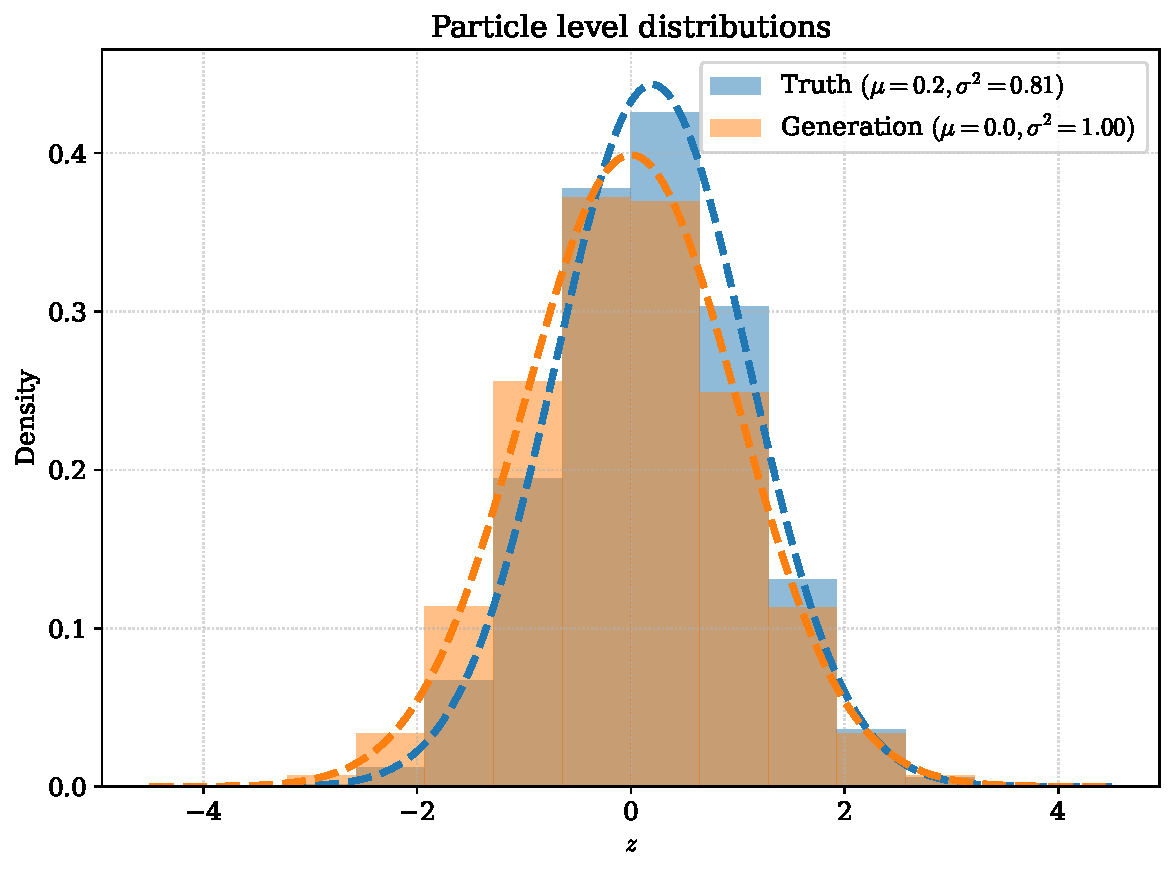
\includegraphics[width=\textwidth]{figures/chapter-07/unbinned_cor-particle_level.pdf}
    \caption{Particle level distributions comparing the Truth (blue) with parameters $\mu_{\text{true}} = 0.2$ and $\sigma^2_{\text{true}} = 0.81$ with the Generation distribution (orange) with parameters $\mu_{\text{prior}} = 0$ and $\sigma^2_{\text{prior}} = 1.00$.
    %
    The histograms represent normalised frequency distributions from $N_{\text{true}} = 10^4$ and $N_{\text{MC}} = 10^5$ samples respectively, while the dashed curves show the corresponding analytical Gaussian probability density functions.}
    \label{fig:particle-level}
  \end{subfigure}
  \hfill
  % (b) detector-level
  \begin{subfigure}[t]{0.48\textwidth}
    \centering
    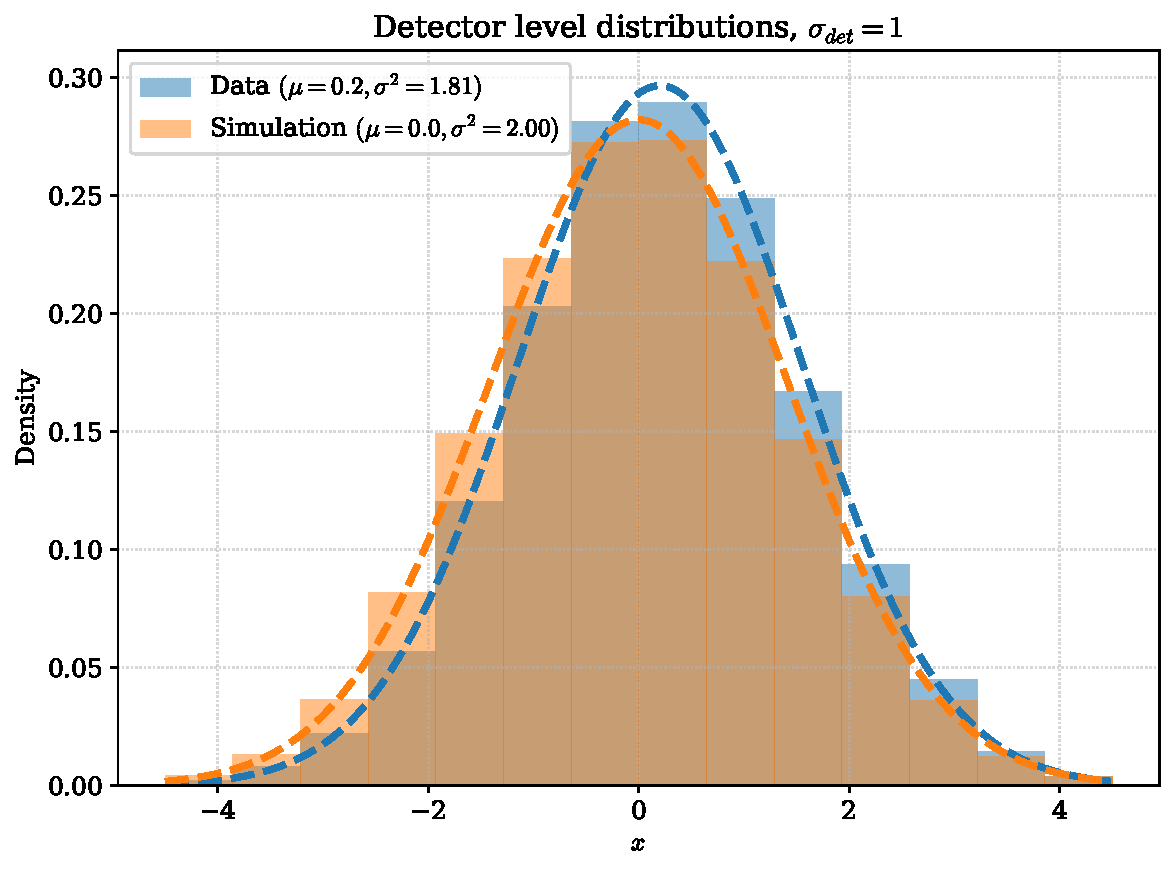
\includegraphics[width=\textwidth]{figures/chapter-07/unbinned_cor-detector_level.pdf}
    \caption{Detector level distributions after applying Gaussian smearing with resolution $\sigma_{\text{det}} = 1.0$. The Data distribution (blue) has parameters $\mu_{\text{data}} = 0.2$ and $\sigma^2_{\text{data}} = 1.81$, while the Simulation distribution (orange) has $\mu_{\text{sim}} = 0$ and $\sigma^2_{\text{sim}} = 2.00$.
    %
    The smearing particle to detector level is Gaussian with $\sigma^2_{\text{det}} = \sigma^2_{\text{particle}} + \sigma^2_{\text{smearing}}$, demonstrating the convolution of detector resolution effects.}
    \label{fig:detector-level}
  \end{subfigure}
  \caption[Detector and particle level distributions for the study on correlations during inference.]{Comparison of particle level and detector level distributions. Panel (a) shows the particle level distributions where the Truth (blue histogram and dashed curve) differs from the Generation (orange histogram and dashed curve). The true distribution is characterized by a shifted mean ($\mu_{\text{true}} = 0.2$) and reduced variance ($\sigma^2_{\text{true}} = 0.81$) compared to the Generation ($\mu_{\text{prior}} = 0$, $\sigma^2_{\text{prior}} = 1.00$).

  
  Panel (b) demonstrates the effect of finite detector resolution through Gaussian smearing with $\sigma_{\text{det}} = 1.0$, which convolves with the underlying distributions to produce broader observed distributions at the detector level.
  %
  The detector-level variances increase according to the quadrature sum $\sigma^2_{\text{detector}} = \sigma^2_{\text{particle}} + \sigma^2_{\text{det}}$, yielding $\sigma^2_{\text{data}} = 1.81$ and $\sigma^2_{\text{sim}} = 2.00$ for the Data and Simulation respectively.
  }
  \label{fig:distributions-1d}
\end{figure}
\begin{figure}
  \centering
  \begin{subfigure}[t]{0.48\textwidth}
    \centering
    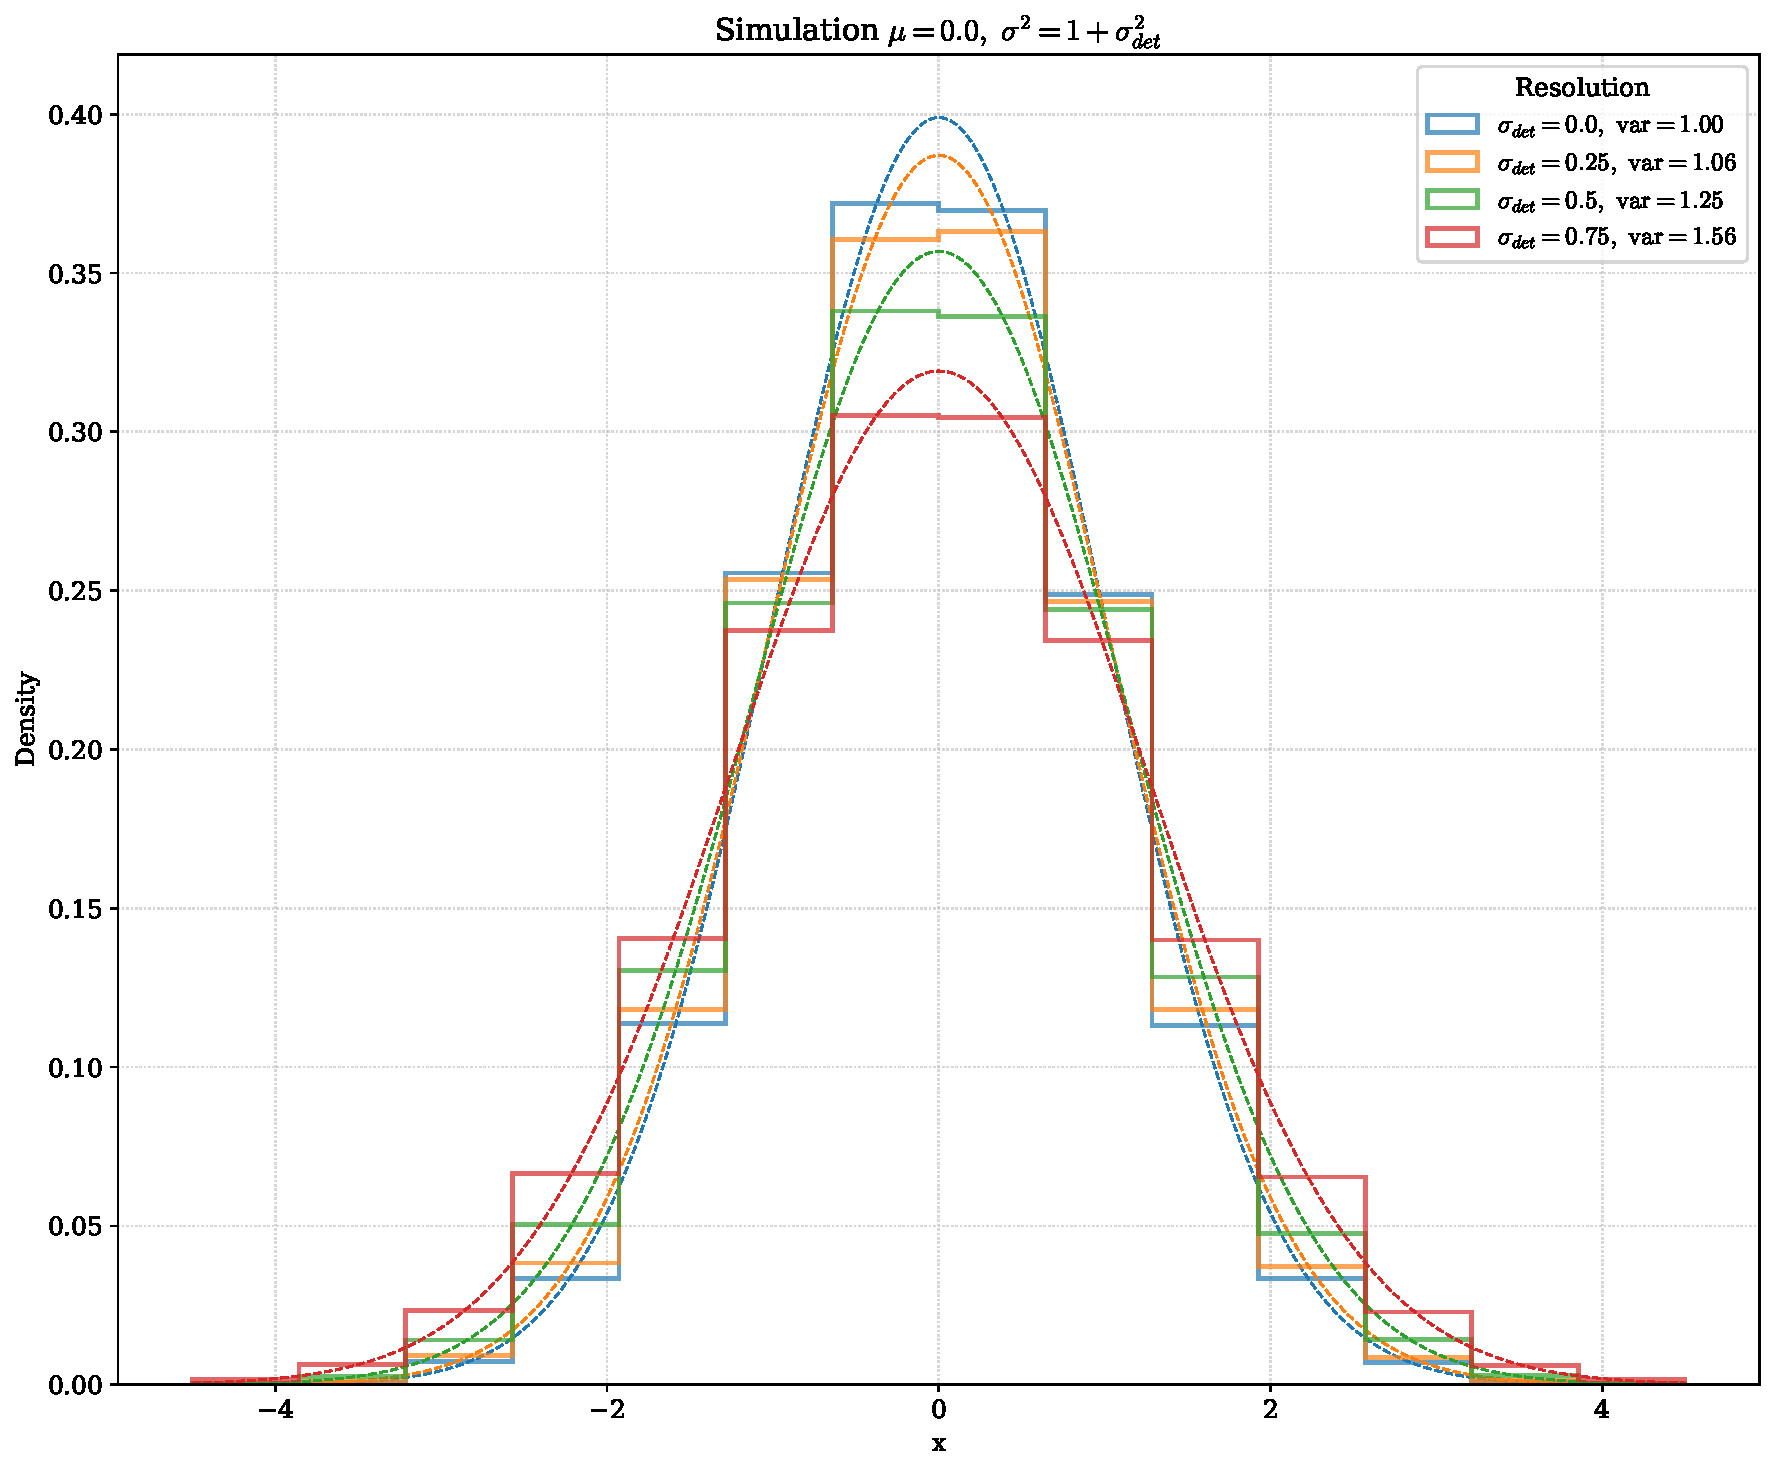
\includegraphics[width=\textwidth]{figures/chapter-07/unbinned_cor-smearing_examples.pdf}
    \caption{Detector level distributions as a function of detector resolution $\sigma_{\text{det}}$.
    %
    Step histograms show the normalised density of Simulation samples ($N = 10^5$) after applying Gaussian smearing with $\sigma_{\text{det}} \in \{0.00, 0.25, 0.50, 0.75\}$. Dashed curves represent the corresponding analytical Gaussian probability density functions with variance $\sigma^2_{\text{total}} = \sigma^2_{\text{MC}} + \sigma^2_{\text{det}} = 1 + \sigma^2_{\text{det}}$.
    %
    The progression from $\sigma_{\text{det}} = 0$ (perfect detector) to $\sigma_{\text{det}} = 0.75$ demonstrates how increasing detector resolution degrades the measurement precision, with total variances ranging from 1.00 to 1.56.}
    \label{fig:smearing-examples}
  \end{subfigure}
  \hfill
  \begin{subfigure}[t]{0.48\textwidth}
    \centering
    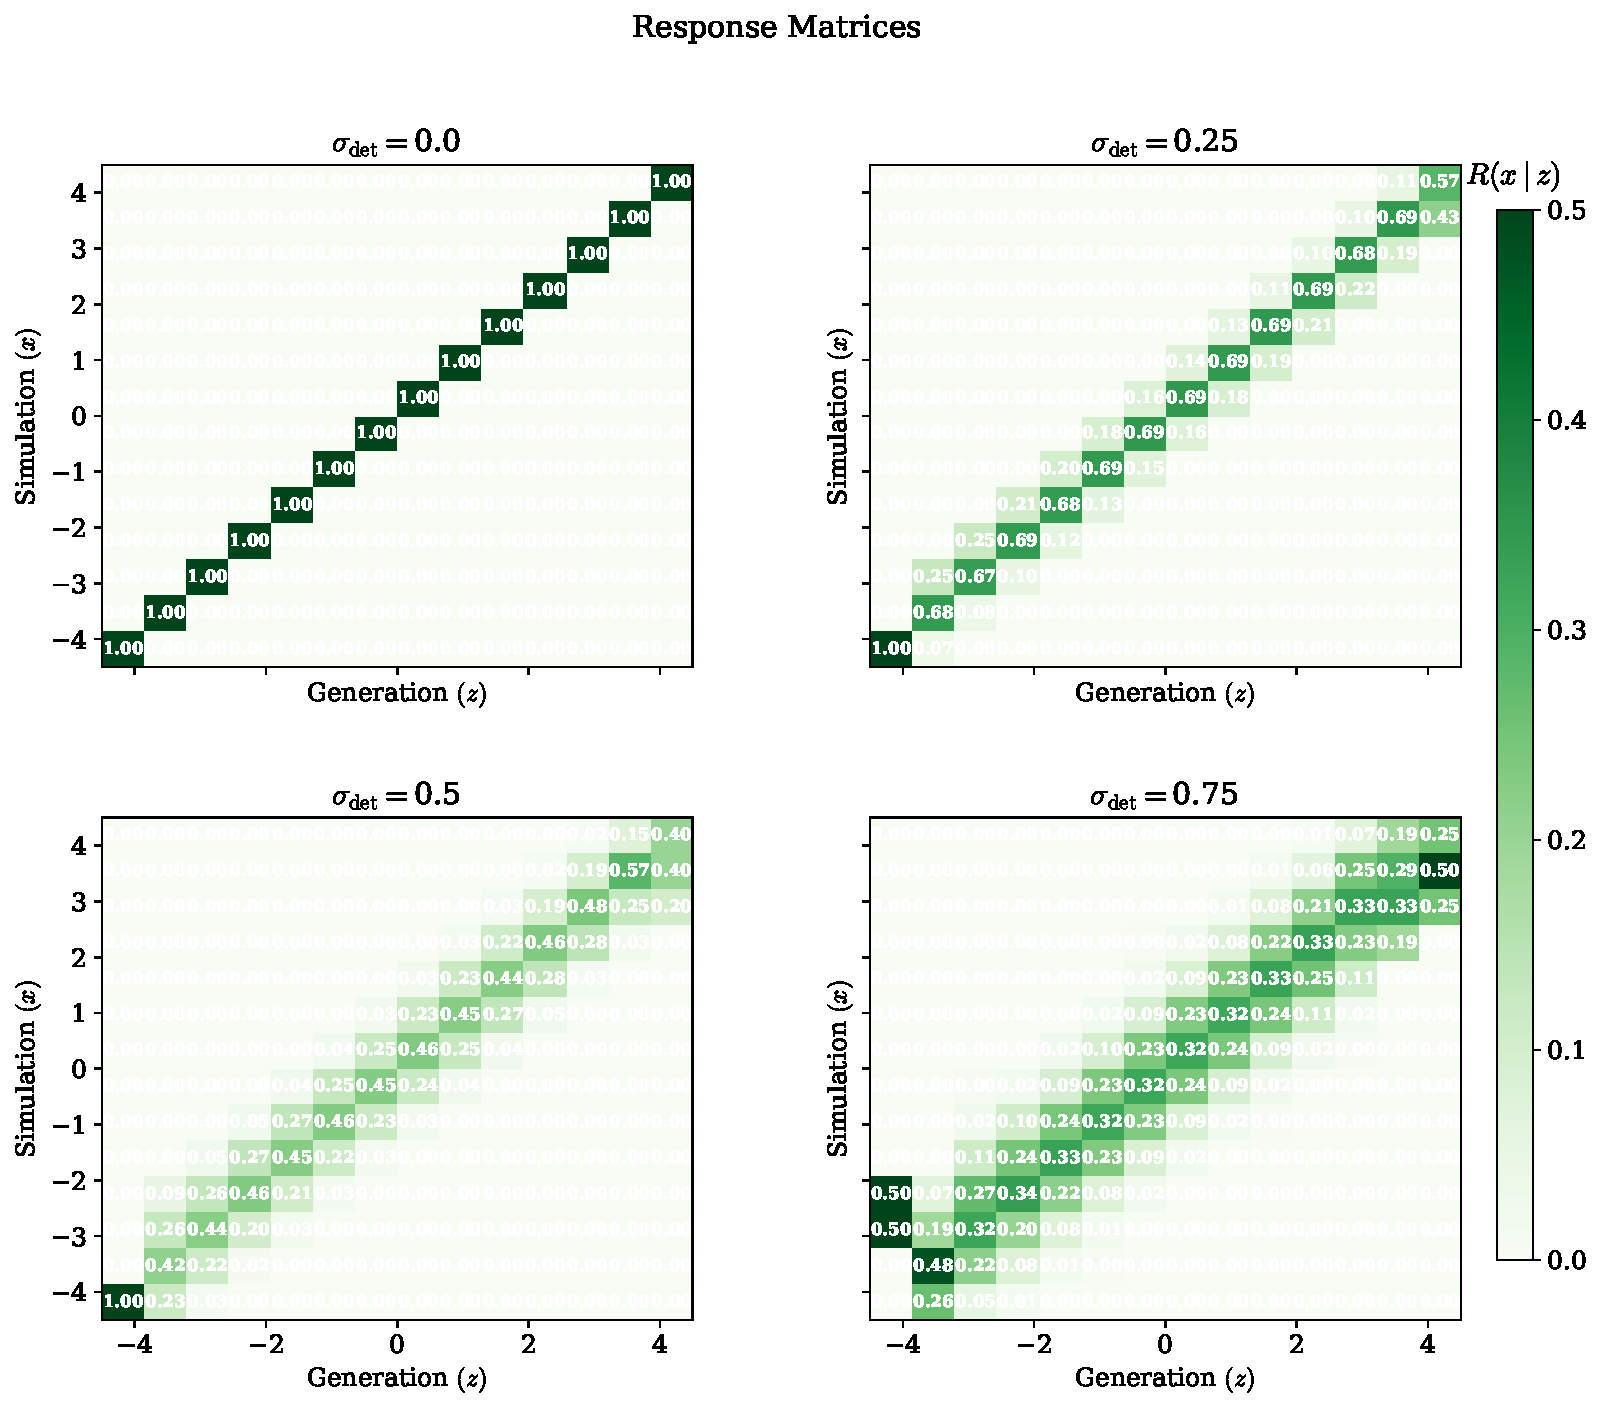
\includegraphics[width=\textwidth]{figures/chapter-07/unbinned_cor-response_matrix.pdf}
    \caption{Discretised response matrices $R(x_i|z_j)$ representing the conditional probability of measuring an event in detector level bin $i$ given that it was generated in particle level bin $j$.
    %
    Each matrix element is normalised such that $\sum_i R(x_i\mid z_j) = 1$ for all $j$.
    The four panels correspond to detector resolutions $\sigma_{\text{det}} \in \{0.00, 0.25, 0.50, 0.75\}$, showing the transition from a diagonal matrix (perfect resolution) to increasingly off diagonal structures as detector smearing increases. Cell values indicate migration probabilities.}
    \label{fig:response-matrices}
  \end{subfigure}
  \caption{Characterisation of detector response effects through progressive smearing of Monte Carlo simulation. Panel (a) illustrates the impact of finite detector resolution on the observed distributions, showing how the Generation is broadened by convolution with Gaussian response functions of width $\sigma_{\text{det}}$. The total observed variance follows the quadrature sum $\sigma^2_{\text{observed}} = \sigma^2_{\text{particle}} + \sigma^2_{\text{det}}$.
  %
  Panel (b) presents the corresponding binned response matrices $R(x_i\mid z_j)$, which encode the probability of bin migration due to detector effects.
  %
  For perfect resolution ($\sigma_{\text{det}} = 0$), the response matrix is diagonal, indicating no bin migration.
  %
  As detector resolution degrades, off diagonal elements become increasingly prominent, quantifying the probability of events generated in bin $j$ being reconstructed in neighbouring bins.
  }
  \label{fig:smearing-and-response}
\end{figure}
            Using the large MC sample, construct a detector response matrix mapping particle level bins to detector level bins.
            %
            Each element $R_{ij}$ of this matrix gives the probability for an event originating in truth bin $i$ to be reconstructed in detector bin $j$.
            %
            In practice, $R_{ij}$ is obtained by binning the MC events by their true and smeared values.
            %
            The response matrix, along with the smeared data histogram, serves as input to the unfolding algorithm.\footnote{In Bayesian terms, the unsmeared MC histogram also provides a prior estimate for the truth distribution.}
            %
            \cref{fig:response-matrices} shows the response matrices estimated using Generation--Simulation pairs for various levels of smearing.
    
            Then apply the IBU algorithm to the binned Data in order to unfold the effects of smearing.
            %
            Starting from the Generation distribution, IBU iteratively updates the estimate of the Truth histogram by comparing the Simulation and Data in the detector space and applying Bayes' theorem to reweight contributions back to particle space. 
            %
            In this study, IBU was iterated for five iterations.
            
            This unfolded result consists of bin counts (or densities) for the truth histogram, along with an estimated covariance matrix for those bin counts.
            %
            The bin--to--bin covariances arise from the finite statistics of the data and from the smearing correlations introduced by the unfolding procedure.
            
            One can estimate the covariance matrix of the unfolded histogram by repeating the unfolding on many statistically independent pseudo experiments, similar to bootstrapping. 
            %
            After unfolding, perform a binned fit to extract the parameters of the underlying distribution (in this case, the Gaussian’s mean $\mu$ and variance $\sigma^2$).
            %
            For each unfolded histogram, a $\chi^2$ minimisation is used to fit a Gaussian model to the unfolded data.
            %
            Importantly, the theoretical Gaussian model is integrated over each bin to yield the expected content in that bin for given values of $\mu$ and $\sigma^2$, so that the comparison between the model and the unfolded histogram is exact with no interpolation or bin centre approximation.
            
            The fit’s $\chi^2$ is computed using the full covariance matrix of the unfolded bins, thereby incorporating all statistical correlations between bins.
            %
            The outcome of the fit is a pair of best--fit parameters $(\hat{\mu}, \hat{\sigma}^2)$ along with their asymptotic uncertainty estimates (\(1\sigma\) intervals) derived from the curvature of the $\chi^2$ at the minimum.
            %
            For comparison, this study also consider a \emph{diagonal covariance} fit, repeating the same procedure but using only the diagonal elements of the covariance, functionally treating unfolded bin counts as if they were independent.
            %
            This allows one to see the impact of neglecting inter--bin correlations on the inferred uncertainties.
            %
            To numerically evaluate the bias, variance, and confidence interval coverage of this procedure, the entire analysis is repeated for each pseudo--experiment.
            
            This ensemble provides a distribution of fitted parameter values $\hat{\mu}$ and $\hat{\sigma}^2$ from which one can quantify the bias, which is the difference between the average fitted value and the true value, the variance or spread of the estimates (related to the expected statistical uncertainty), and the empirical coverage of confidence intervals.
            %
            In practice, one could alternatively use bootstrapping on a single dataset to assess these metrics; indeed, this study has also checked that bootstrapped replicas yield consistent uncertainty estimates as the independent toys, confirming that the ensemble size is sufficient.

            Use the above procedure to obtain an unfolded result and fit for each pseudo--experiment.
            %
            One can now examine the bias and variance of the estimates.
\begin{figure}
    \centering
    % (a) mu uncertainty
    \begin{subfigure}[t]{0.48\textwidth}
        \centering
        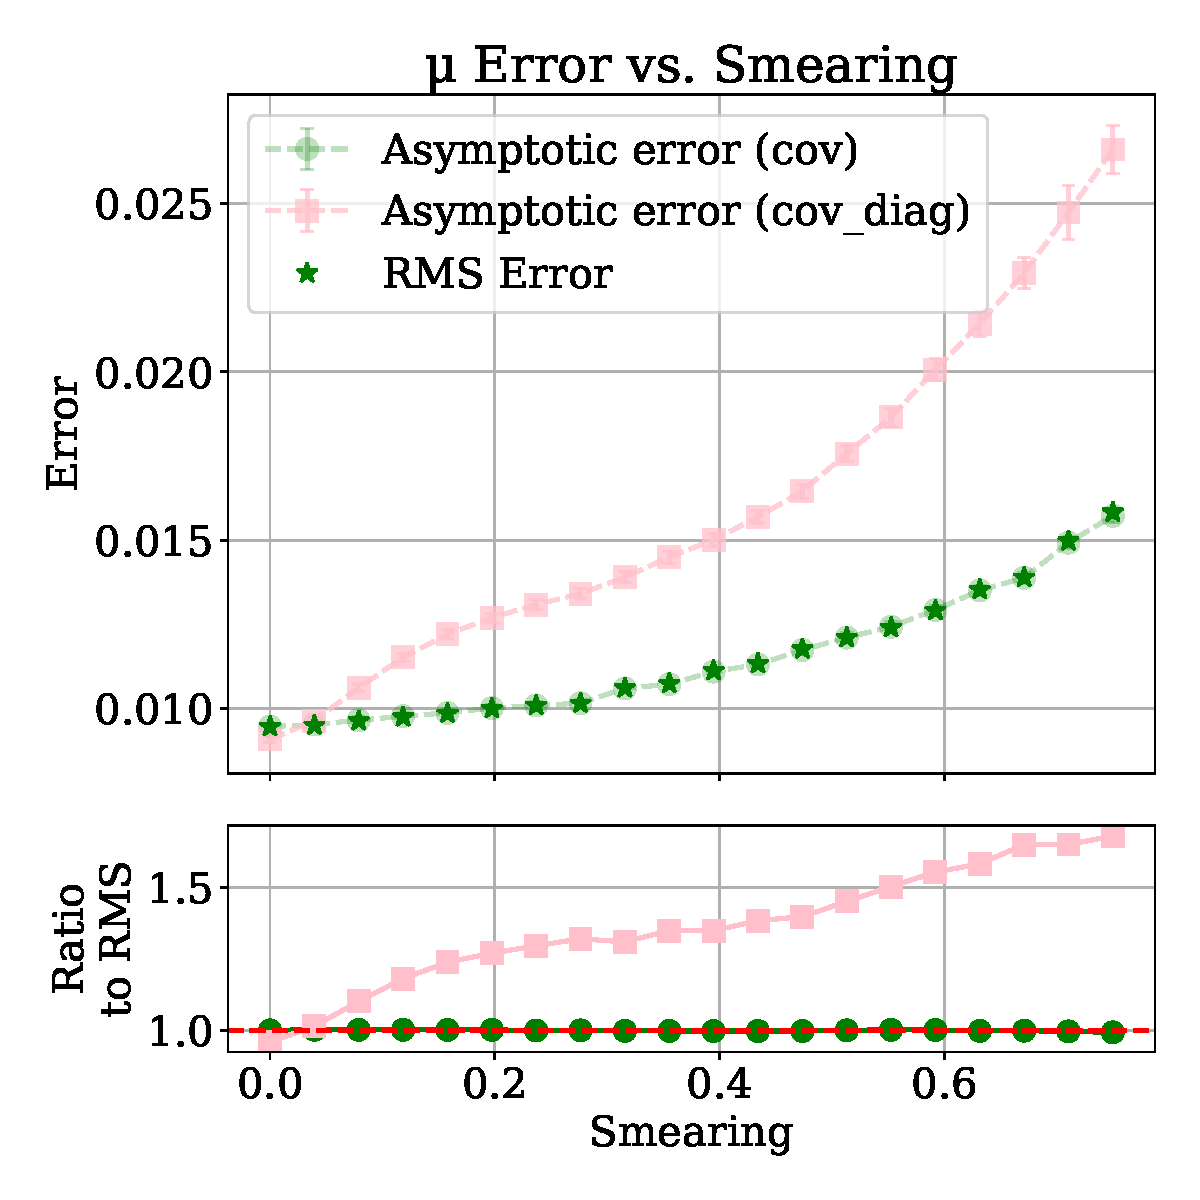
\includegraphics[width=\textwidth]{figures/chapter-07/mu_error_plot_with_errorbars_ratio.pdf}
        \caption{Asymptotic uncertainty on the Gaussian mean parameter $\mu$ as a function of detector resolution $\sigma_{\text{det}}$.
        %
        The lower panel displays the ratio of diagonal to full covariance uncertainties, demonstrating systematic overestimation by factors reaching 1.4 at $\sigma_{\text{det}} = 1.0$.}
        \label{fig:mu_error_plot_with_errorbars}
    \end{subfigure}
    \hfill
    % (b) variance uncertainty
    \begin{subfigure}[t]{0.48\textwidth}
        \centering
        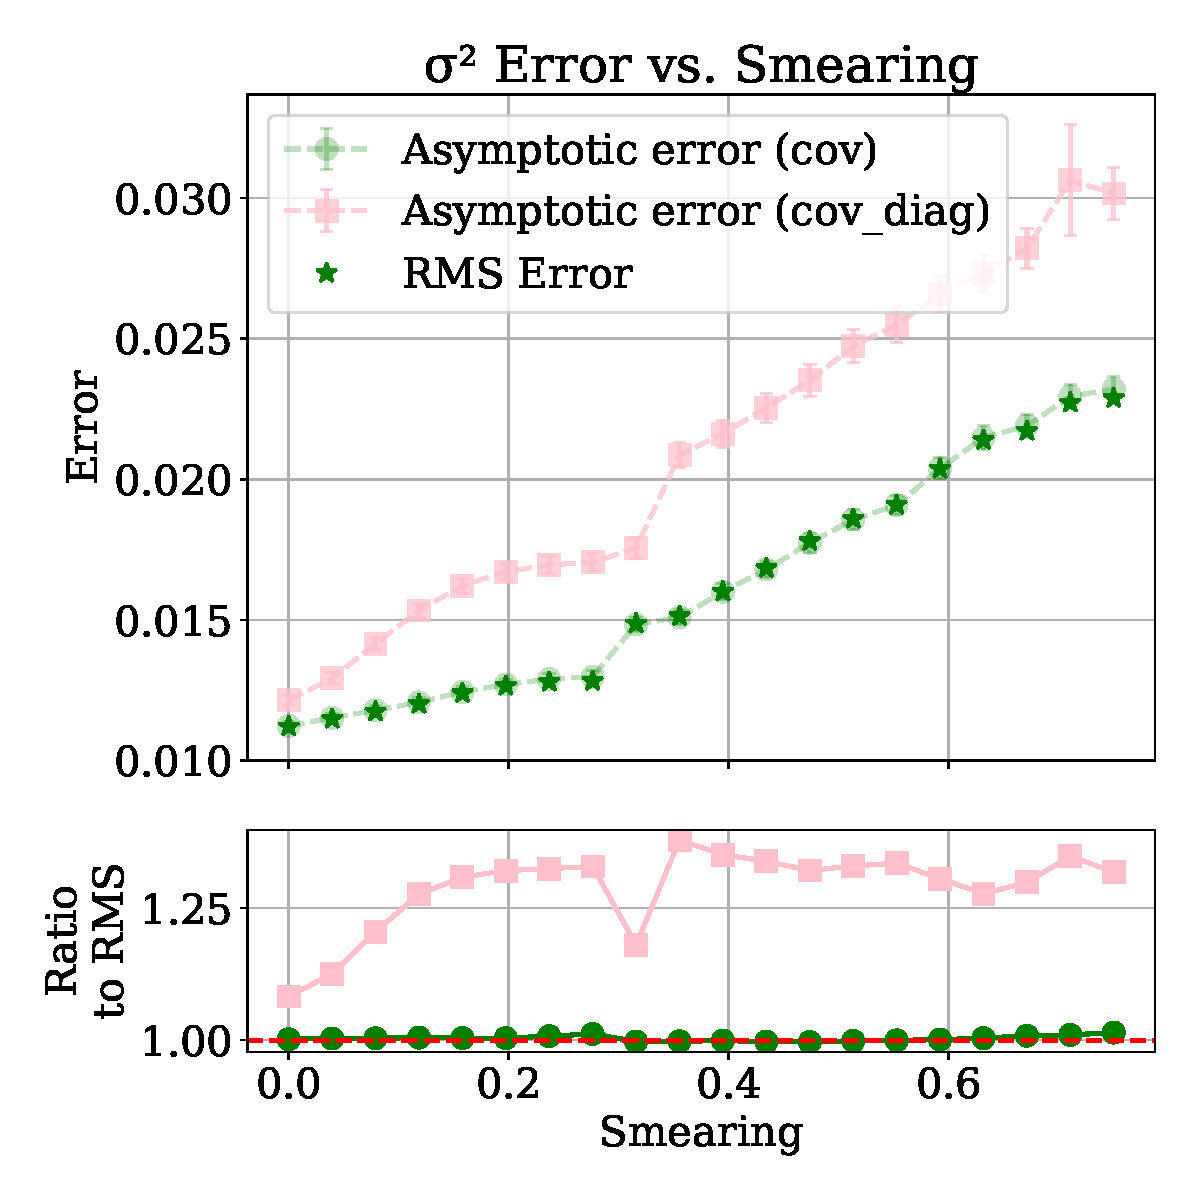
\includegraphics[width=\textwidth]{figures/chapter-07/var_error_plot_with_errorbars_ratio.pdf}
        \caption{Asymptotic uncertainty on the variance parameter $\sigma^2$ as a function of detector resolution $\sigma_{\text{det}}$.
        %
        The diagonal approximation increasingly overestimates the uncertainty as detector resolution degrades, with the ratio reaching approximately 1.5 at $\sigma_{\text{det}} = 1.0$, indicating that neglecting bin correlations leads to measurable over-coverage.}
        \label{fig:var_error_plot_with_errorbars}
    \end{subfigure}
    \caption[Comparison of uncertainty estimation methods for binned unfolded distribution parameters as a function of detector resolution.]{Comparison of uncertainty estimation methods for binned unfolded distribution parameters as a function of detector resolution. Panels (a) and (b) show the asymptotic uncertainties for the Gaussian mean $\mu$ and variance $\sigma^2$ parameters, respectively. The analysis compares three approaches: (i) full covariance matrix treatment accounting for all correlations (green circles), (ii) diagonal covariance approximation that neglects off-diagonal terms (pink squares), and (iii) empirical validation through 500 independent pseudo-experiments (green stars). The excellent agreement between the full covariance asymptotic errors and bootstrap derived uncertainties validates the analytical error propagation framework. The diagonal approximation consistently overestimates uncertainties, with the discrepancy growing monotonically with detector smearing. This overestimation arises from neglecting negative correlations between bins introduced by the normalisation constraint in the unfolding procedure. Proper treatment of the full covariance structure is essential for when extracting distribution parameters through subsequent fits.}
    \label{fig:uncertsfullybinned}
\end{figure}

\begin{figure}
    \centering
    \begin{subfigure}[t]{0.48\textwidth}
        \centering
        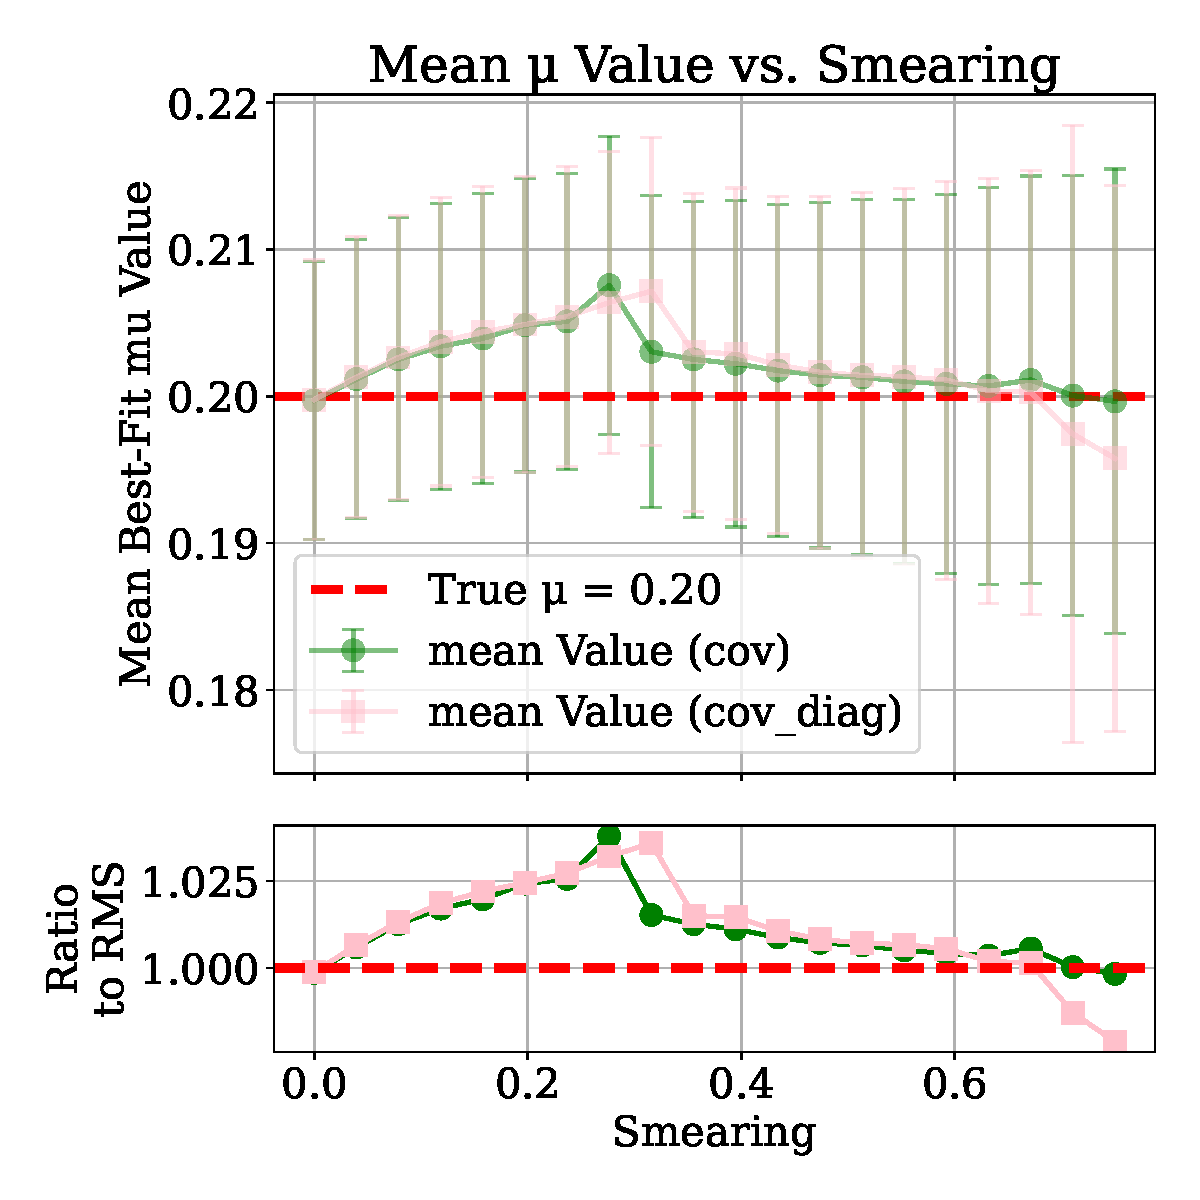
\includegraphics[width=\textwidth]{figures/chapter-07/mu_mean_values_with_errorbars_ratio.pdf}
        \caption{Mean best-fit values of the Gaussian mean parameter $\mu$ as a function of detector resolution $\sigma_{\text{det}}$.
        %
        The lower panel shows the ratio to truth, demonstrating unbiased parameter extraction within statistical uncertainties across all detector resolutions.}
        \label{fig:mu_mean_values_with_errorbars}
    \end{subfigure}
    \hfill
    % (b) variance central values
    \begin{subfigure}[t]{0.48\textwidth}
        \centering
        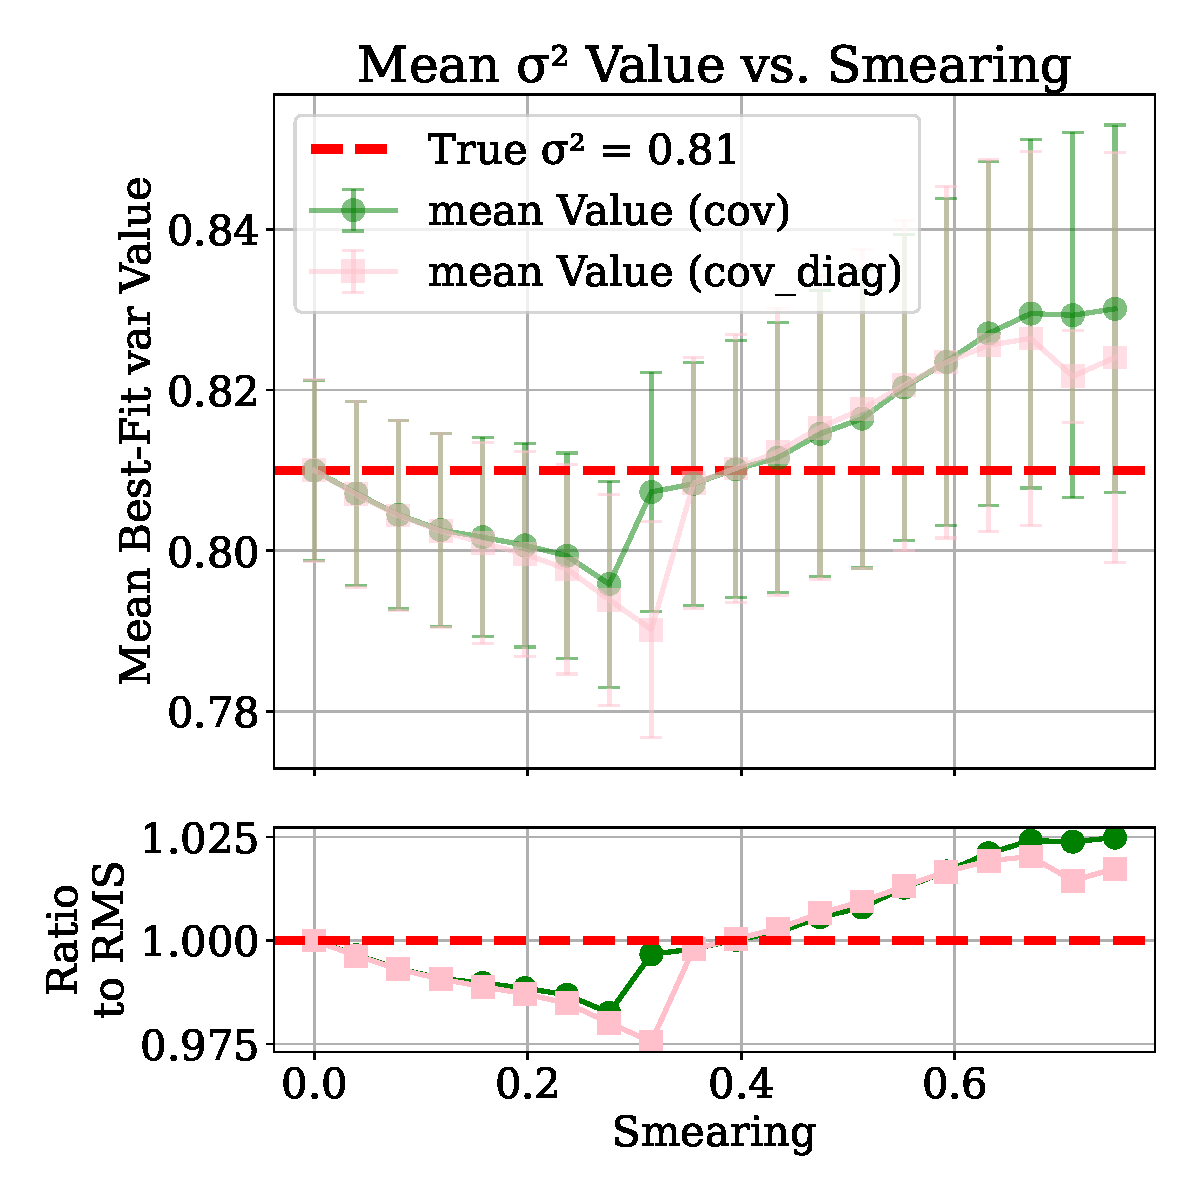
\includegraphics[width=\textwidth]{figures/chapter-07/var_mean_values_with_errorbars_ratio.pdf}
        \caption{Mean best-fit values of the variance parameter $\sigma^2$ as a function of detector resolution $\sigma_{\text{det}}$. The presentation follows panel (a). The slight systematic trend toward misestimation at large $\sigma_{\text{det}}$ may arise from regularization bias in the unfolding procedure or finite binning effects.}
        \label{fig:var_mean_values_with_errorbars}
    \end{subfigure}
    \caption[Validation of unbiased parameter extraction from unfolded distributions across varying detector resolutions.]{Validation of unbiased parameter extraction from unfolded distributions across varying detector resolutions. Panels (a) and (b) display the mean best-fit values for the mean $\mu$ and variance $\sigma^2$ parameters, respectively, obtained by fitting unfolded distributions from 500 independent pseudo-experiments. The analysis demonstrates that both the full covariance matrix treatment (green circles) and diagonal approximation (pink squares) yield unbiased central values, recovering the true parameters (red dashed lines: $\mu_{\text{true}} = 0.2$, $\sigma^2_{\text{true}} = 0.81$) within statistical uncertainties across the full range of detector resolutions tested.
    %
    Error bars represent the standard error of the mean over the ensemble of pseudo-experiments, quantifying the precision. The ratio panels confirm parameter recovery within uncertainties, of truth values, validating the unfolding procedure's ability to correct for detector effects without introducing systematic biases. The consistency between full and diagonal covariance approaches for central values indicates that while correlation treatment significantly impacts uncertainty estimation, it does not affect the the point estimates.
    }
    \label{fig:centralvaluesfullybinned}
\end{figure}
            The analysis is repeated for each value of the detector resolution $\sigma_{\text{det}}\in[0, 0.75]$ to see how worsening detector effects impact the inference.
            %
            \cref{fig:mu_mean_values_with_errorbars} and \cref{fig:var_mean_values_with_errorbars} summarize the accuracy or bias of the method, showing the mean fitted $\mu$ and $\sigma^2$ across 500 trials as a function of the detector smearing.
            %
            Figure\ref{fig:uncertsfullybinned} focuses on the precision and uncertainty coverage, comparing the nominal 1$\sigma$ errors from the fits to the actual spread of the results.
            %
            These results demonstrate that the IBU unfolding followed by a proper binned fit recovers the true distribution parameters without significant bias.
            %
            For all tested smearing levels, the average fitted mean $\langle \hat{\mu}\rangle$ remains within statistical uncertainty of the true value, \(0.2\), and the average fitted variance $\langle \hat{\sigma}^2\rangle$ within statistical uncertainty of \(0.81\).
            %
            In Fig.\ref{fig:mu_mean_values_with_errorbars} and Fig.\ref{fig:var_mean_values_with_errorbars}, the averaged best fit values lie on or around the horizontal red dashed lines marking the true parameters.
            %
            The deviations are well within the statistical error bars\footnote{the standard error of the mean over the 500 trials}, indicating no significant bias in the unfolding or fitting procedure.
            %
            Notably, the choice of using the full covariance versus only diagonal uncertainties in the fit has no effect on the central values obtained.
            %
            Both approaches yield correct $\hat{\mu}$ and $\hat{\sigma}^2$, which might be explained by the bias in this context being dominated by any unfolding imperfections and IBU, with sufficient iterations, being an asymptotically unbiased estimator of the truth distribution.
    
            When using the full covariance matrix in the $\chi^2$ fit, the asymptotic uncertainty estimates for $\hat{\mu}$ and $\hat{\sigma}^2$ are found to be in excellent agreement with the actual distribution of fit results across the ensemble.
            %
            In \cref{fig:uncertsfullybinned}, the green circle markers show the average $1\sigma$ uncertainties from the fits (i.e. the fit errors from the covariance matrix of each fit) as a function of detector resolution.
            %
            These are virtually indistinguishable from the green star markers, which indicate the empirical RMS standard deviation of the 500 fitted values at each resolution.
            %
            In other words, the fit’s error estimates accurately predict the trial--to--trial fluctuations of the outcomes.
            %
            This agreement implies that the reported 68\% confidence intervals have the correct coverage:
            %
            approximately 68\% of the pseudo--experiments' $\hat{\mu}$ (or $\hat{\sigma}^2$) results lie within $\pm1\sigma$ of the true value, as expected for well calibrated uncertainties.
            %
            As the detector resolution worsens, the uncertainty on the inferred parameters grows, reflecting the loss of information, but at each point, the full covariance \(\chi^2\) fit's uncertainty remains an accurate representation of the actual variance in the results.
    
            If one ignores the off--diagonal elements of the unfolded covariance matrix and assumes the bins are independent, the inferred uncertainties become misestimated.
            %
            In this example, neglecting the negative bin--to--bin correlations from unfolding leads to an overestimation of the parameter errors.
            %
            The pink square markers in Fig.~\ref{fig:uncertsfullybinned} show the average fit uncertainty on $\mu$ and $\sigma^2$ obtained when using only the diagonal uncertainties.
            %
            These are significantly larger than both the true ensemble spread (green stars) and the full covariance asymptotic errors (green circles) once any non-zero smearing is present.

            %
            This overly conservative error estimate would lead to over-coverage of confidence intervals.
            %
            The nominal 68\% interval contains the true value substantially more than 68\% of the time.
            
            This indicates an inefficient use of information.
            %
            The fit is effectively double--counting fluctuations in each bin that in reality are anti--correlated with fluctuations in other bins.
            %
            These findings reinforce that incorporating the full covariance matrix from the unfolding is essential to obtaining reliable and correctly sized confidence intervals in the fully binned approach, and suggests that this may be the case in unbinned approaches too.
            
        In summary, this study in the fully binned regime demonstrates that a conventional unfolding approach (IBU) combined with rigorous statistical treatment produces unbiased and well calibrated inference of physics parameters.
        %
        The unfolded results, when analysed with their full covariance matrix, give parameter estimates whose uncertainties accurately reflect the true spread across experiments, ensuring correct confidence interval coverage.
        %
        The study also shows that simplifying assumptions like treating unfolded bins as independent can skew the uncertainty estimates, in this case, making them overly conservative, even though the point estimates remain correct.
        %
        These findings provide a firm baseline for comparison with the unbinned methods discussed in the next sections.
        %
        After a brief detour to discuss correlation diagnostics after unbinned unfolding, following section will investigate how unbinned unfolding techniques handle event correlations and whether they can achieve a similar level of statistical reliability as this fully binned approach.
        %
        The lessons learned here, particularly the necessity of accounting for induced correlations, will carry forward as one transitions to unbinned inference on correlated data.
        
    \subsection{Correlation diagnostics after unbinned unfolding}
    \label{subsec:weight_correlations}
        Before confronting any inference procedure with an unbinned output, one must first quantify the statistical dependencies that the unfolding induces.
        %
        This subsection introduces two complementary diagnostics that make those correlations both visible and quantifiable.
        \begin{enumerate}
            \item The \textbf{pairwise weight–-distance correlation} $\rho(|x_i-x_j|)$ between all pairs unfolded events $i$ and $j$, and
            \item The \textbf{bin--bin covariance matrix} $C_{ab} = \operatorname{Cov}[\,\vb*{\nu}_a,\vb*{\nu}_b\,]$ of a fine histogram binned {after} unfolding.
        \end{enumerate}
        Both are evaluated for four detector resolutions $\sigma_{\det}\in\{0,0.25,0.50,0.75\}$ and for two distinct estimators, {KDE} and neural network (\textsc{NN}) conditional density estimators.

\begin{figure}
    \centering
    % Store the footnote counter
    \setcounter{footnote}{18}  % Set to whatever the current number should be minus 1
    % (a) KDE correlations
    \begin{subfigure}[t]{\textwidth}
        \centering
        \includegraphics[width=0.95\textwidth]{figures/chapter-07/weight-correlation-vs-distance-1d-set1.pdf}
        \caption{KDE based \textsc{OmniFold}: Weight correlations decay exponentially with separation distance, maintaining values of $\sim$0.1 at distances of 2--3 units for $\sigma_{\text{det}} = 0.75$~\cite{Desai:2025mpy}.\footnotemark}
        \label{fig:weight-corr-kde}
    \end{subfigure}
    \stepcounter{footnote}
    \begin{subfigure}[t]{\textwidth}
        \centering
        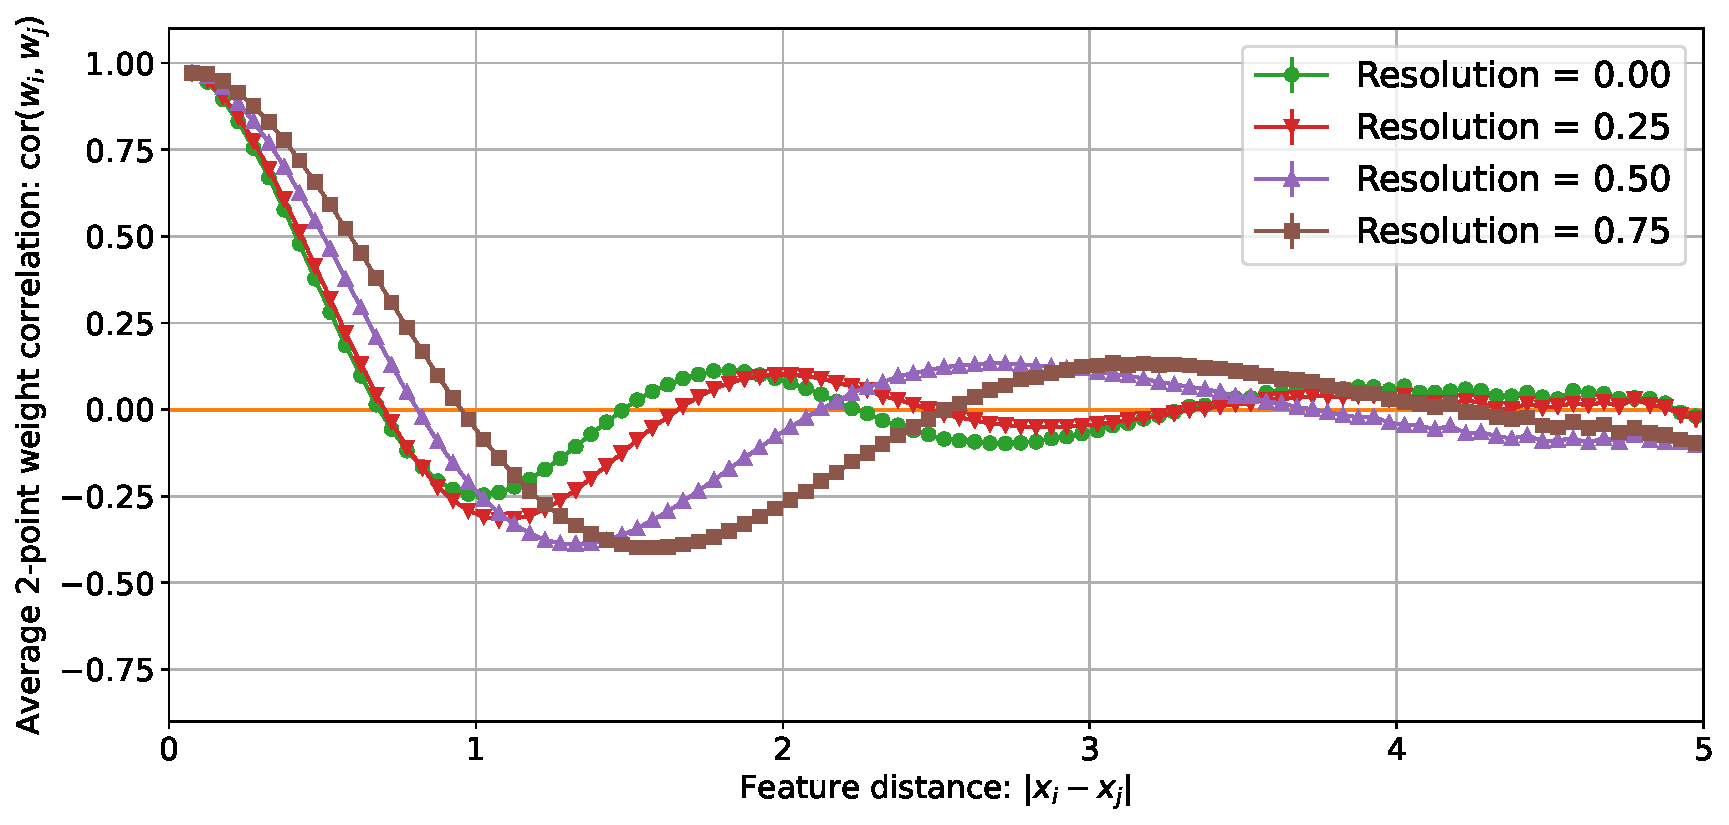
\includegraphics[width=0.95\textwidth]{figures/chapter-07/weight-correlation-vs-distance-1d-set2.pdf}
        \caption{NN-based \textsc{OmniFold}: Weight correlations exhibit rapid decay, becoming negligible beyond $|x_i - x_j| \approx 1$ for all detector resolutions~\cite{Desai:2025mpy}.\footnotemark}
        \label{fig:weight-corr-nn}
    \end{subfigure}
    \caption[Event wise weight correlations as a function of separation distance for different unfolding methods.]{Average pairwise correlation between unfolding weights as a function of absolute distance $|x_i - x_j|$ between events in the observable space. Both panels show results $\sigma_{\text{det}} \in \{0.00, 0.25, 0.50, 0.75\}$. Error bars represent the RMS variation of correlation values within each distance bin. Panel (a) shows the KDE approach which exhibits more localised correlations. Panel (b) displays the neural network (NN) method, which produces longer-range correlations. The characteristic correlation length scales approximately linearly with detector resolution. These correlation patterns have important implications for statistical analyses of unfolded data.
    }
    \label{fig:weight-correlation-vs-distance-1d}
\end{figure}
\addtocounter{footnote}{-2}
\footnotetext{Figure produced by Owen Long~\cite{Desai:2025mpy}.}
\stepcounter{footnote}
\footnotetext{Figure produced by Owen Long~\cite{Desai:2025mpy}.}

        The results are displayed in \cref{fig:weight-correlation-vs-distance-1d} and \cref{fig:weight-histogram-covariance-1d}, respectively, and form the empirical basis for the coverage study in \cref{subsec:unbinned_data}.
        
        \subsubsection{Pairwise weight--distance correlations}
        For every event, by considering the weight distributions across pseudo--experiments one can compute the correlation coefficient, defined as
        \[
            \rho_{ij} = \frac{\mathrm{Cov}(w_i,w_j)}{\sigma_{w_i}\,\sigma_{w_j}}
        \]
        One can then average $\rho_{ij}$ in bins of $\Delta x = |x_i-x_j|$, where $x$ is the unfolded observable.\footnote{
            %
            The average is taken after combining results from 500 pseudo–experiments; error bars in \cref{fig:weight-correlation-vs-distance-1d} denote the ensemble RMS of $\rho_{ij}$ in each $\Delta x$ bin, thereby incorporating both the statistical fluctuation correlations and any run-‐to-‐run variability of the unfolding.
            }
            %
            A few different features of the resulting curves in \cref{fig:weight-correlation-vs-distance-1d} (\cref{fig:weight-corr-kde} for {KDE}, \cref{fig:weight-corr-nn} for {NN}) are worth nothing.
            \begin{itemize}
            \item \textbf{Perfect detector ($\sigma_{\det}=0$):}
                %
                One should expect the average pairwise correlation to be $\rho(|\Delta x|) \simeq 0$ for all separations $\Delta x>0$, confirming that when no smearing is applied, \textsc{OmniFold} reproduces the {factorised likelihood} limit in which event weights are statistically independent~\cite{andreassen_omnifold_2020,Milton:2025mug}.
                %
                At $\Delta x = 0$ we trivially should expect $\rho(0)=1$ because every event is, of course, perfectly correlated with itself.
                %
                In both \cref{fig:weight-corr-kde, fig:weight-corr-nn}, it is correctly the case that \(\rho(0) = 1\) and \(\rho(|\Delta x| \gg 1 \simeq 0.\)
                
                In the truly ideal i.i.d. case, one would expect the fall off from $\rho(0)=1$ to $\rho(|\Delta  x|>0) = 0$ to resemble a Dirac $\delta$ at the origin.
                %
                The {KDE} estimator indeed approaches this limit.
                %
                Its kernel bandwidth determines a correlation length \(\ell \lesssim\!0.15\).\cite{2006AllStatistics, wand_kernel_1994}.
                %
                By contrast, even with extensive experimentation with architecture and hyperparameter tuning one finds that {NN} priors leave a residual plateau $\rho\approx0.75$ around $\ell\approx1$, which then leads to the damped oscillatory structure of the correlation curve.
                %
                One could speculate about reasons why unfolding with neural networks even in the perfect detector resolution case should lead to correlated weights.
                %
                Two potential explanations are
                \begin{enumerate}
                    \item \emph{Network smoothness:} the shared weights in the neural network classifier impose a finite ``receptive field,''~\cite{miller_information-theoretic_1995, djolonga_robustness_2021, saratchandran_weight_2024} causing nearby events to receive similar gradient updates and hence correlated weights; and
                    \item \emph{Global normalisation:} \textsc{OmniFold} enforces $\sum_i w_i = N_{\text{MC}}$ at every iteration.
                    %
                    This normalisation might be introducing a weak positive correlation of size $1/N$ even in the absence of detector effects~\cite{cowan_highlights_2011,1937PropertiesTests}.
                \end{enumerate}
                Although numerically tiny, this effect, whatever its underlying explanation sets the optimistic lower bound on variance reduction when working with neural networks.
                %
                Thus even the idealised zero--smearing case does not yield perfectly independent weights in practice, a useful caution when quoting statistical uncertainties from inference using ML processed data.
            \item \emph{Mild smearing (\(\sigma_{\det}=0.25\)):}
                %
                Short range correlations of order \(\rho\gtrsim 0.5\) appear for \(\Delta x\lesssim0.4\).
                %
                These are already sufficient to reduce the {effective sample size}
                \[
                  N_{\text{eff}} = \frac{N}{1+(N-1)\rho}
                  \]
                  considerably.
                  %
                  \(\rho < 0\) for \(\Delta \in [1, 2]\), as expected.
                  %
                  For both the NN and the KDE, \(\rho\) exhibits the same damped oscillatory structure, as would be expected by the normalization imposed by the unfolding.
                  %
                  \(\ell_{\text{KDE}}\) is noticeably smaller that \(\ell_{\text NN}\).
                  %
                  The contrast is less pronounced than in the perfect-resolution case, yet still visible.
            \item \emph{Moderate and large smearing ($\sigma_{\det}\ge0.5$):}
                % 
                Correlations develop a broad plateau {independent of distance}.
                %
                In that regime $N_\text{eff}$ collapses explaining why a naïve fit ignoring  correlations would significantly misestimate errors.
            \end{itemize}
            The \textsc{NN} generally yields more long range, but {slightly weaker} correlations than the \textsc{KDE} at the same resolution, suggesting that a higher capacity estimator might be able to better absorb detector noise. 
            %
            However, the qualitative behaviour is identical;
            any non-zero smearing produces, long range weight correlations that violate the i.i.d. assumption built into standard unbinned likelihoods.
        \subsubsection{Histogram covariance matrices.}
            Since most downstream analyses eventually bin the unfolded events, a histogram covariance matrix can be effective to visualize the correlations.
            %
            The impact on such \emph{binned} summaries can be visualised by filling a 40 bin histogram in the range $[-4,4]$ for each pseudo--experiment and computing
            \[
              C_{ab} = \bigl\langle
                         (N_a-\bar N_a)(N_b-\bar N_b)
                       \bigr\rangle.
            \]
            %
            The matrices, shown in \cref{fig:weight-histogram-covariance-1d}, reinforce the observations from the correlation curves.
            %
            Even at zero smearing, while KDE produces a nearly diagonal $C_{ab},$ \textsc{OmniFold}'s weights exhibit small but noticable off diagonal elements.
            %
            Growing the smearing leads to pronounced \emph{anti--correlations} along the first off diagonal and coherent positive correlations far from the diagonal.
            %
            For $\sigma_{\det}=0.75$ the largest off diagonal coefficient reaches $|\rho_{ab}|\simeq0.5$, echoing the plateau seen in $\rho(|\Delta x|)$.  These patterns are almost identical for KDE and NN analyses.

            Such strong off diagonal structure rigorously explains why a $\chi^2$ fit that ignores covariances by using only the diagonal of $C$ leads to significant miscoverage.
\begin{figure}
    \centering
    \begin{subfigure}[b]{\textwidth}
        \centering
        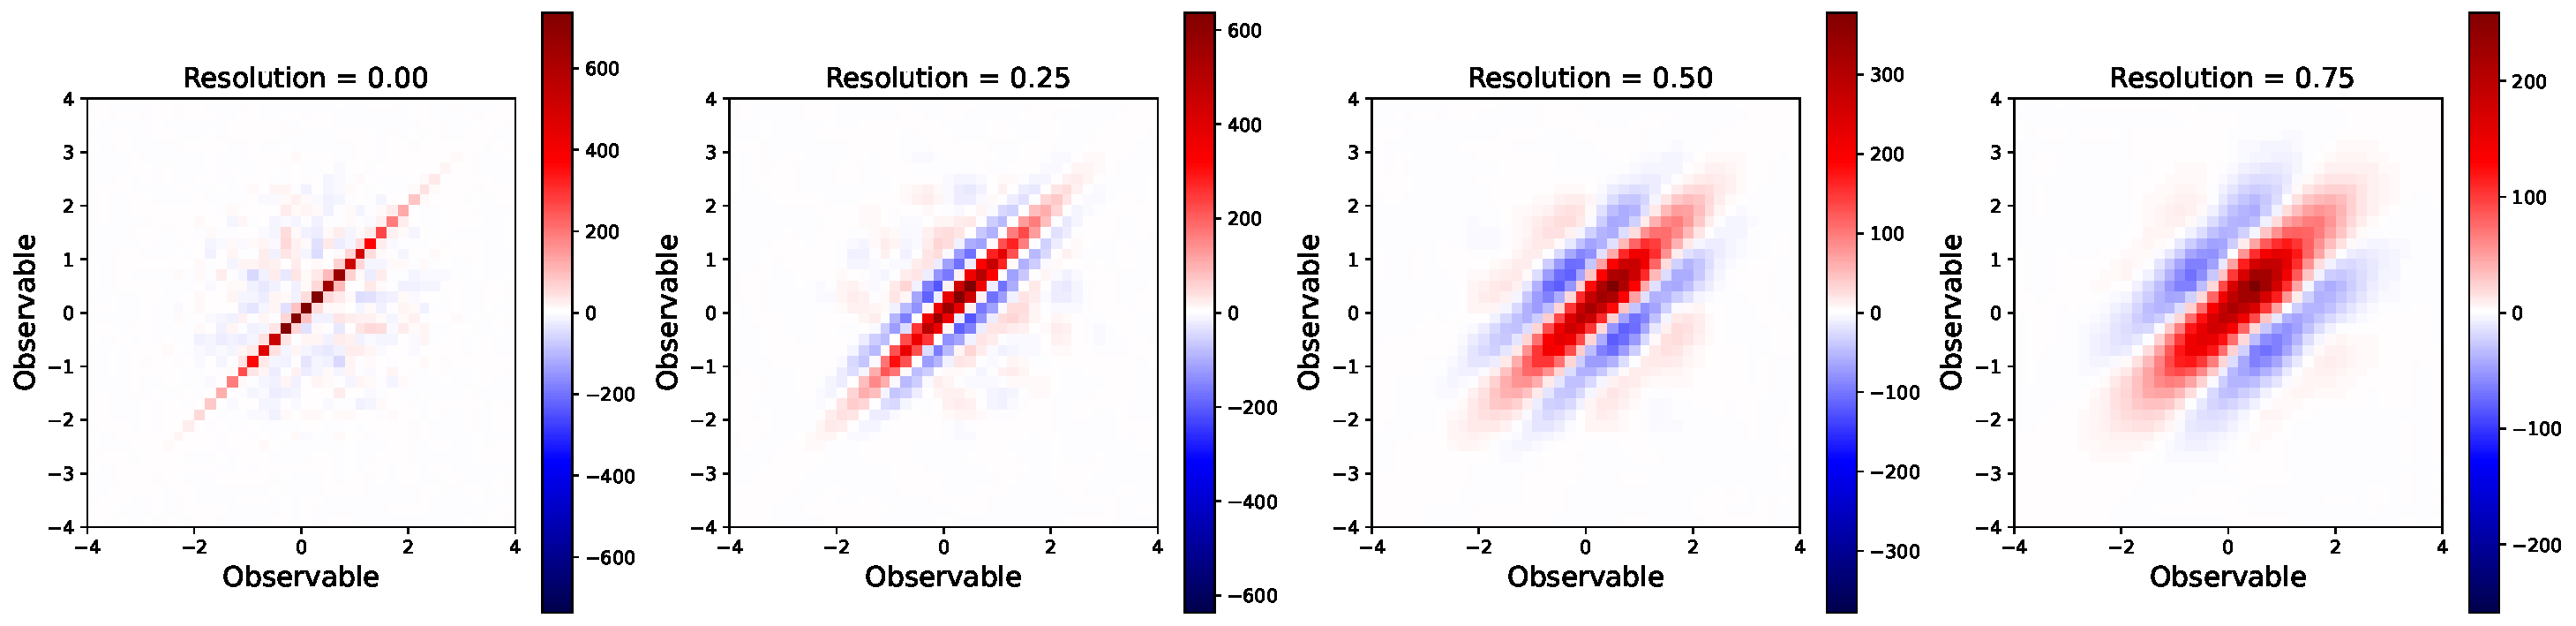
\includegraphics[width=0.95\textwidth]{figures/chapter-07/weight-histogram-covariance-1d.pdf}
        \caption{KDE-based \textsc{OmniFold}: Covariance matrices exhibit concentrated correlation structures with significant values ($>0.1$) confined primarily to nearest and next to nearest neighbour bins.\footnotemark}
        \label{fig:covar-kde}
    \end{subfigure}
    \stepcounter{footnote}
    \begin{subfigure}[b]{\textwidth}
        \centering
        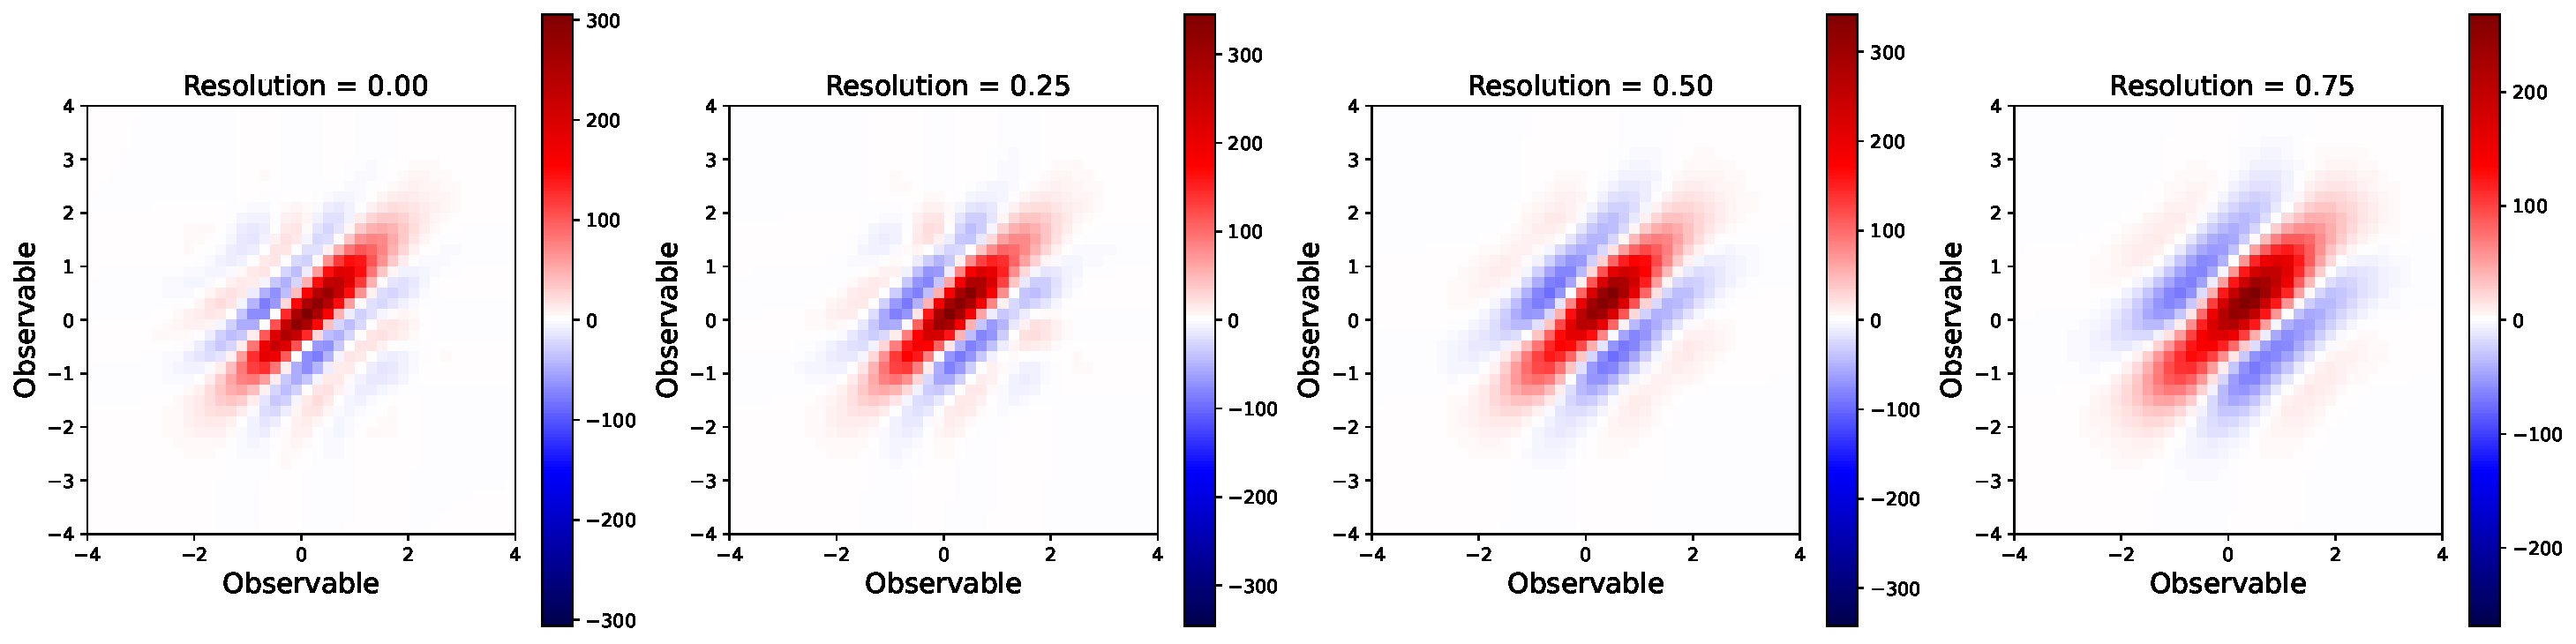
\includegraphics[width=0.95\textwidth]{figures/chapter-07/weight-histogram-covariance-1d-nn.pdf}
        \caption{NN-based \textsc{OmniFold}: Covariance matrices exhibit broad correlation bands extending $\ge10$ bins from the diagonal at $\sigma_{\text{det}} = 0.75$.\footnotemark}
        \label{fig:covar-nn}
    \end{subfigure}
    \caption[Covariance structure of binned unfolded distributions for KDE and NN-based methods.]{Covariance matrices of binned histograms constructed from unfolded distributions for $\sigma_{\text{det}} \in \{0.00, 0.25, 0.50, 0.75\}$. Each axis represents the covariance structure of a 40--bin histogram over $[-4, 4]$ in the observable space, with bin width $\Delta x = 0.2$. Matrix elements $\rho_{ij}$ represent the correlation between bins $i$ and $j$.
    %
    Panel (a) displays results from KDE and Panel (b) shows NN results, both using the \textsc{OmniFold} method. Both methods exhibit a clear progression from nearly diagonal matrices at perfect resolution to increasingly correlated structures as detector resolution degrades.
    %
    The integrated correlation strength, sum of absolute off-diagonal elements, increases approximately quadratically with $\sigma_{\text{det}}$, reflecting the information loss that must be compensated through correlated adjustments.
    %
    These covariance matrices are essential inputs for rigorous statistical analysis of unfolded data, and must be propagated through any subsequent fits or hypothesis tests to obtain correct uncertainties.}
    \label{fig:weight-histogram-covariance-1d}
\end{figure}
\addtocounter{footnote}{-2}
\footnotetext{Figure produced by Owen Long~\cite{Desai:2025mpy}.}
\stepcounter{footnote}
\footnotetext{Figure produced by Owen Long~\cite{Desai:2025mpy}.}
        \subsubsection{Implications}
            The correlation diagnostics presented here {empirically validate} the theoretical expectation that \textsc{OmniFold} weights are correlated.
            %
            Quantifying the strength and range of those correlations enables a rough estimate of how badly an independence based error formula will fail.
            %
            With these diagnostics in hand, one is now equipped to benchmark the statistical performance of binned and unbinned inference workflows on unbinned unfolded data.
    \subsection{Unbinned unfolding: binned and unbinned inference.}
    \label{subsec:unbinned_data}
        Having established a fully binned baseline in \cref{subsec:fully_binned_demo}, this section examines two inference workflows that utilise unbinned unfolding on the same Gaussian data.
        %
        Both approaches start by unfolding the detector level data without binning, producing a set of weighted events at truth level.
        %
        Because the deconvolution process induces non-negligible correlations between event weights as evidenced by the covariance patterns in \cref{fig:weight-correlation-vs-distance-1d,fig:weight-histogram-covariance-1d}, these workflows differ in how they handle those correlations.
    
        When performing binned inference on unbinned unfolded data, the unfolded weighted events are aggregated into a histogram, and a binned template fit is performed using a $\chi^2$ statistic that includes the full binned covariance matrix.
        %
        In this workflow the unfolded distribution is fit to the parametric Gaussian model with mean $\mu$ and variance $\sigma^2$ by integrating the model prediction over the histogram bins.
        %
        The covariance matrix of the bins is estimated from an ensemble of repeated pseudo--experiments.
        
        One then obtains best fit parameters by $\chi^2$ minimisation and determines their uncertainties via the usual $\Delta\chi^2=1$ criterion.
        %
        This approach is analogous to a standard binned analysis except that the data have been unfolded using an unbinned method.
        %
        In this was this workflow offers a statistically rigorous method to propagate the full unfolding--induced covariance into the fit.
    
        Alternatively, one could attempt to fit the parametric model directly to the weighted events using an unbinned maximum likelihood procedure that ignores inter--event correlations.
        %
        One constructs the weighted negative log--likelihood,
        \[
            \operatorname{NLL}(\theta) = -\sum_{i=1}^N w_i \log p(x_i \mid \theta),
        \]
        where $x_i$ and $w_i$ are the kinematic value and weight of event $i$, and $p(x_i|\theta)$ is the model density for parameters $\theta=(\mu,\sigma^2)$.
        
        This unbinned likelihood sum is maximised to obtain the best fit $\hat\theta$.
        %
        The Hessian (curvature) of the NLL at the optimum provides an asymptotic error estimate for $\theta$.
        %
        Equivalently, one finds the $\Delta\ln L=0.5$ offset for a $1\sigma$ interval.
        
        This workflow assumes statistical independence of events~\cite{cowan_survey_2002, Blobel:2011fih, Blobel2013Unfolding}.
        %
        Thus, while method the latter method yields a fit and a formal error bar, these must be interpreted with caution since the underlying likelihood model is misspecified.
    
        Both of the above approaches are applied to the same Gaussian datasets described earlier in \cref{subsec:setup}.
        %
        Unfolding is performed with the \textsc{OmniFold} algorithm.
        %
        In the one dimensional setting a KDE based implementation is also tested.
        %
        For each resolution setting, the 500 pseudo--data samples are unfolded and then subjected to both the aforementioned inference procedures.
        %
        This allows a comparison of the bias, uncertainty estimation, and coverage of the two workflows against the fully binned baseline.
        \subsubsection{Parameter bias}
\begin{figure}
    \centering
    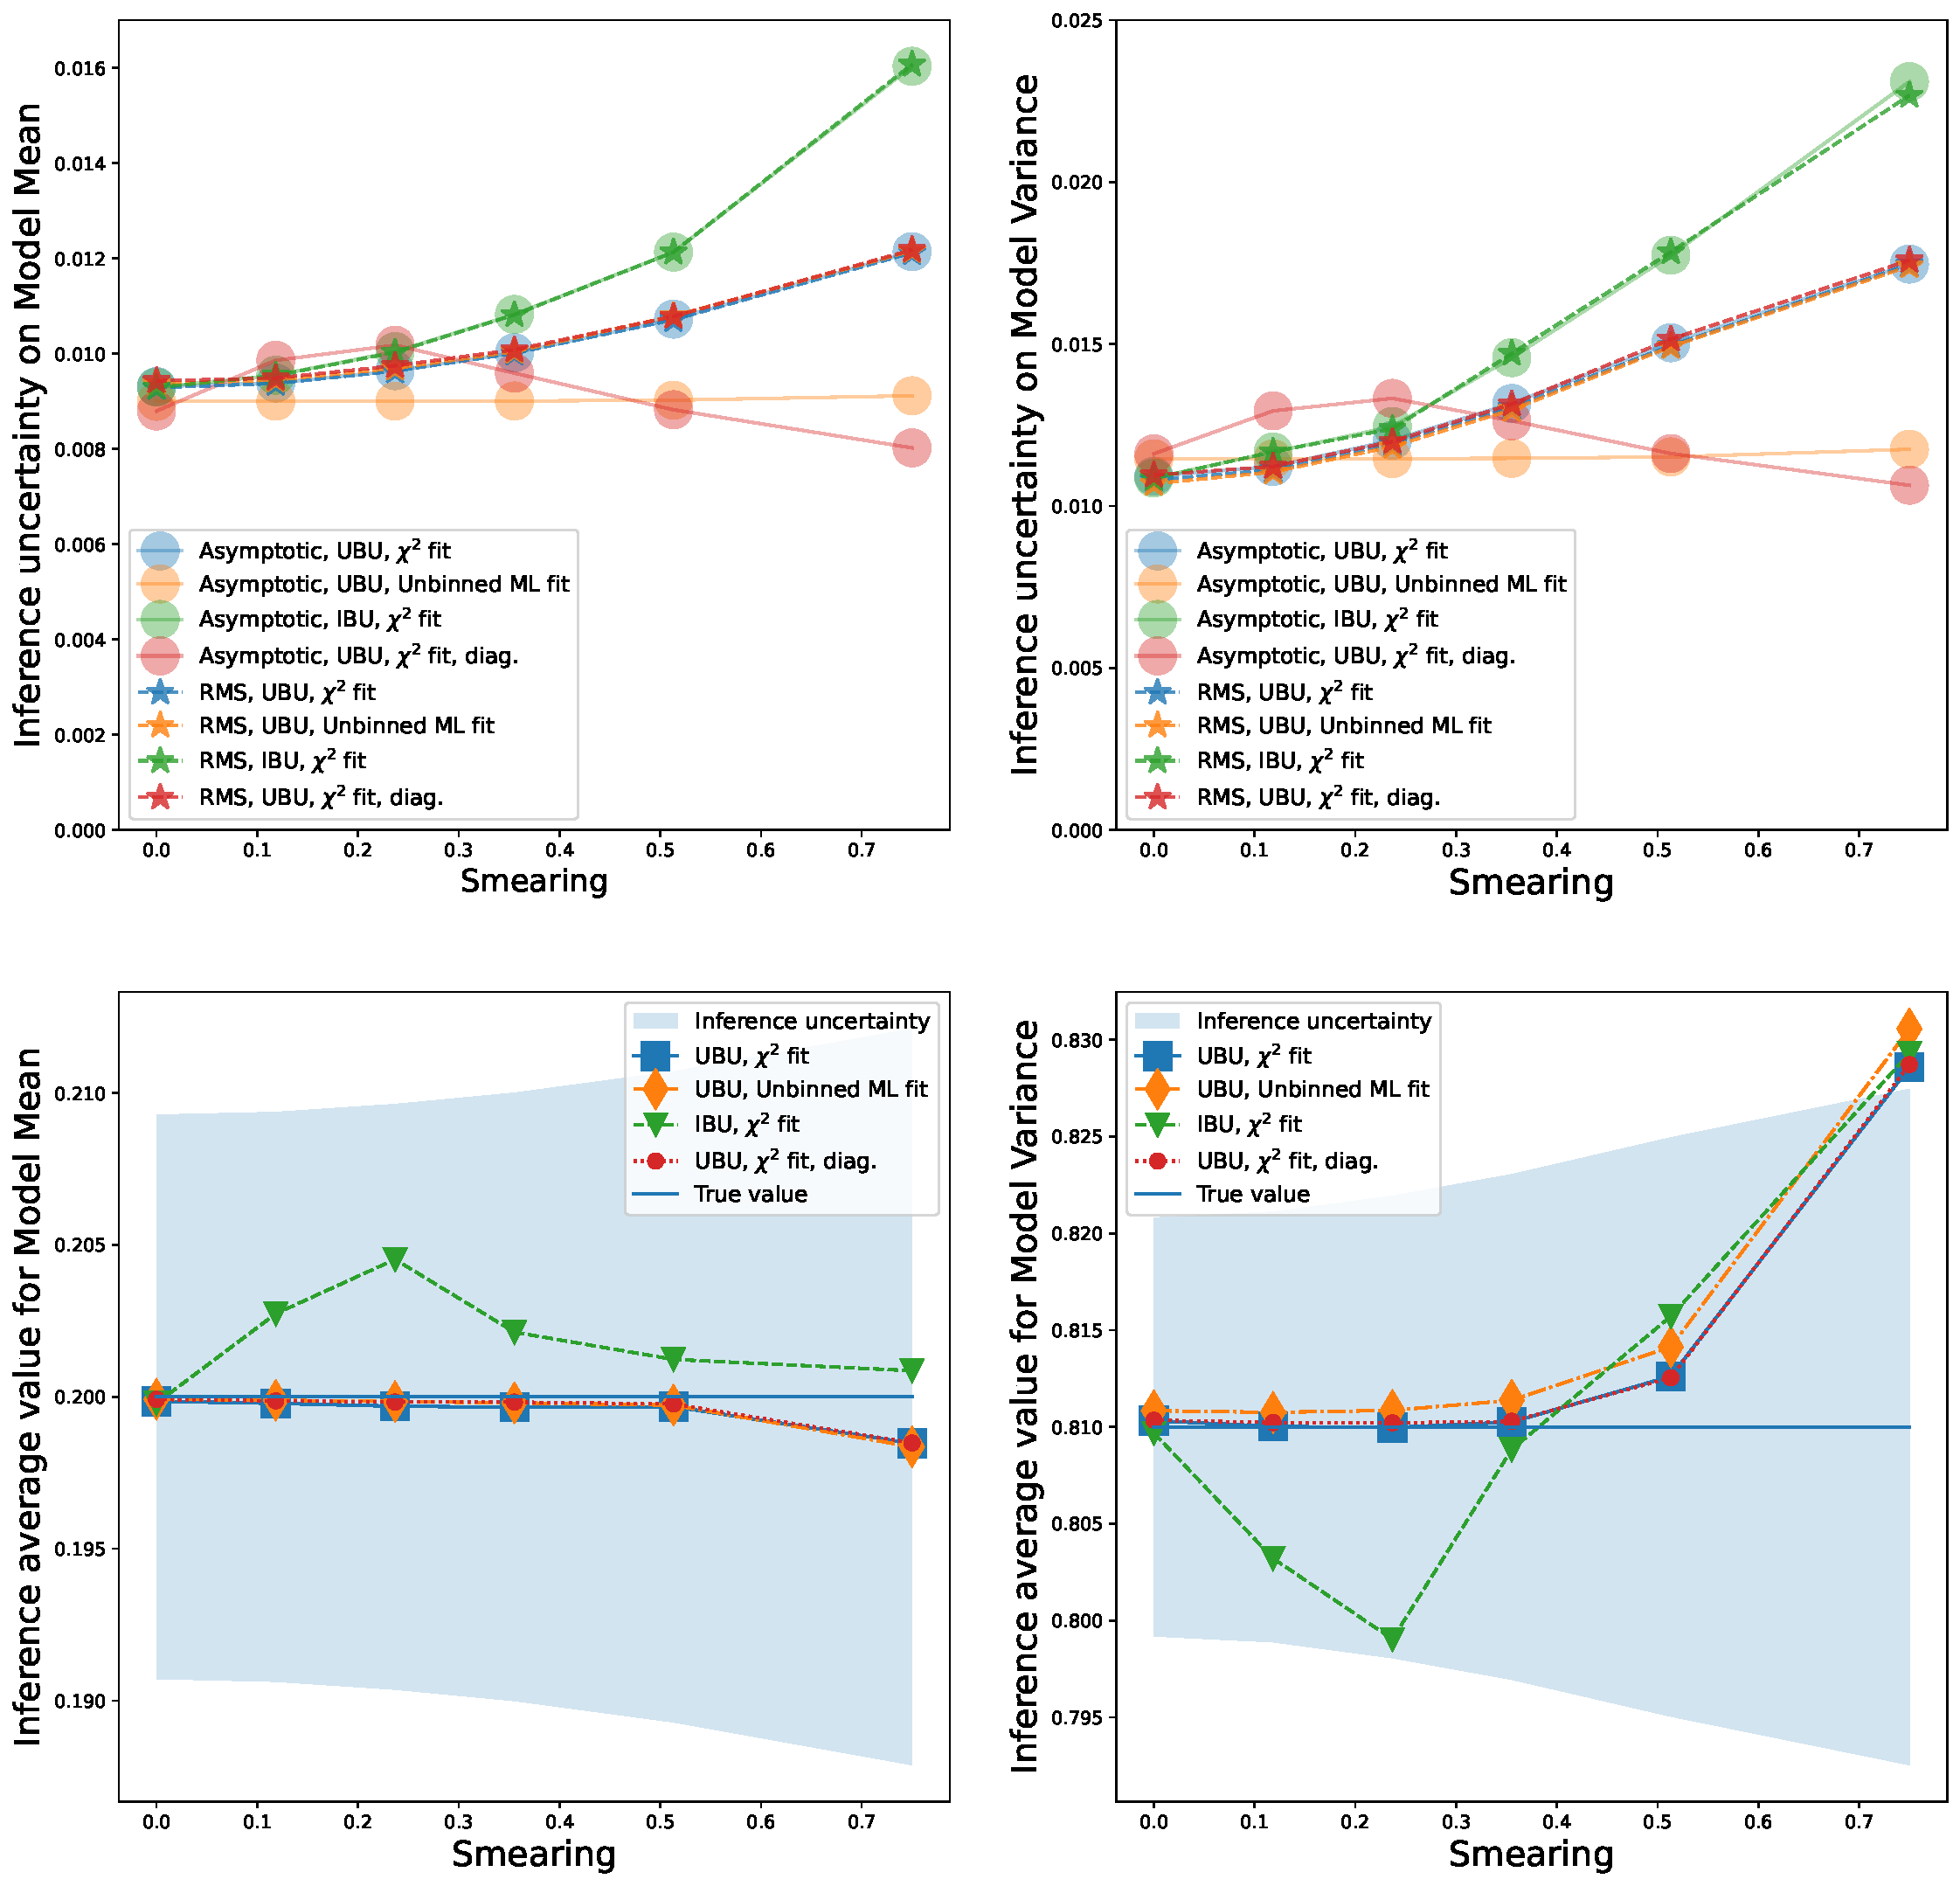
\includegraphics[width=0.95\linewidth]{figures/chapter-07/uncertainty-and-bias-vs-resolution-ibu-diag.pdf}
    \caption[Comparison between binned and unbinned parameter inference with unbinned and binned unfolding methods as a function of detector resolution.]{Systematic comparison of inference uncertainty and bias for distribution parameters extracted from unfolded data as a function of $\sigma_{\text{det}}$.
    %
    (Top left) uncertainty on $\mu$, (top right) uncertainty on $\sigma^2$, (bottom left) bias in $\mu$ estimation, and (bottom right) bias in $\sigma^2$ estimation.
    %
    Three unfolding and inference approaches are compared: (i) Unbinned Unfolding (UBU) with unbinned maximum likelihood (ML) fitting shown as blue circles, (ii) binned Iterative Bayesian Unfolding (IBU) with $\chi^2$ fitting using the full covariance matrix (orange triangles), and (iii) IBU with $\chi^2$ fitting using only diagonal covariance elements (green squares). The blue shaded band in each panel represents $\pm$ RMS inference uncertainty from the UBU+ML approach.\footnotemark
}
    \label{fig:uncertainty-and-bias-vs-resolution}
\end{figure}
\footnotetext{Figure created by Owen Long~\cite{Desai:2025mpy}.}
            Both unbinned workflows yield fitted parameter values that are consistent with those from the binned baseline.
            %
            There is no appreciable bias introduced by the unbinned unfolding step or the choice of inference method.
            %
            \cref{fig:uncertainty-and-bias-vs-resolution} (bottom panels) shows the mean fitted $\mu$ and $\sigma^2$ as a function of detector smearing for each method.
            %
            These results demonstrate the strength of unbinned methods when feasible, while validating that properly implemented binned unfolding with full covariance treatment can achieve comparable performance.
            
            The bias panels (bottom) reveal that all methods maintain bias levels below 1\% of the parameter values for $\sigma_{\text{det}} < 0.5$, with UBU exhibiting the most stable performance.
            %
            At all detector resolutions, IBU shows comparable or larger bias in variance estimation than UBU, but the inferred parameters are still well within statistical uncertainties.
            %
            Indeed, approaches produce estimates of $\mu$ and $\sigma^2$ across the range of smearings within the statistical uncertainties (blue shaded).
            
            Notably, the bias observed in the naive unbinned ML fit is the same as that in the proper $\chi^2$ fit that accounts for the covariance of a given dataset. 
            %
            This can be explained as both fits ultimately maximizing a likelihood, or minimizing a $\chi^2$, to match the unfolded distribution to the model;
            %
            if the model is correctly specified, the MLEs should coincide.
            %
            Thus, unbinned unfolding does not itself induce a bias in the extracted physics parameters verifying the claim that the \textsc{OmniFold} procedure correctly reproduces the shape of the true distribution on average.
            %
            This is demonstrated by the agreement of fitted values with the true parameter shown by the horizontal lines in \cref{fig:uncertainty-and-bias-vs-resolution} and the baseline results in \cref{fig:mu_mean_values_with_errorbars}. 
            
        \subsubsection{Uncertainty estimation and coverage.}
            In sharp contrast to the agreement in central values, the two workflows differ markedly in their reported uncertainties and the statistical coverage of those uncertainties.
            %
            The binned $\chi^2$ approach with full covariance proves to be consistent with the baseline in its uncertainty estimates.
            %
            For each smearing level, the asymptotic $1\sigma$ errors obtained from the $\Delta\chi^2=1$ criterion agree well with the empirical spread (RMS) of the fitted parameters over the \(\num{500}\) pseudo--experiments.
            %
            This is illustrated in the top panels of \cref{fig:uncertainty-and-bias-vs-resolution}: the curve corresponding to the full covariance $\chi^2$ fit lies on top of the true uncertainty obtained from the pseudo data ensemble (star markers), for both $\mu$ (left) and $\sigma^2$ (right).
            %
            In other words, binned inference on unbinned data using a \(\chi^2\) fit that incorporates the full covariance matrix produces accurate confidence intervals that maintain the nominal coverage.
            
            These uncertainty panels (top) demonstrate that an unbinned asymptotic maximum likelihood (ML) fit on unbinned unfolded (UBU) data consistently underestimates statistical uncertainties across all detector resolutions, and is most similar to the results of of performing an asymptotic binned \(\chi^2\) fit on the same UBU results while ignoring off diagonal covariance element.
            %
            The uncertainty degradation with increasing $\sigma_{\text{det}}$ follows the expected $\sqrt{1 + \sigma^2_{\text{det}}/\sigma^2_{\text{true}}}$ scaling for both parameters.

            This behaviour is as expected and desired.
            %
            By incorporating the complete covariance matrix of the unfolded histogram, the binned asymptotic \(\chi^2\) fit on UBU results correctly accounts for the event correlations in the statistical inference, and precisely matches the RMS uncertainty computed numerically on UBU results.
            
            In one sense, these results agree with the fully binned study.
            %
            Recall that in the baseline binned analysis, using the full covariance matrix yielded uncertainty estimates consistent with the bootstrap pseudo--data spread, whereas using only diagonal uncertainties did not, as shown in \cref{fig:uncertsfullybinned}.
            %
            \cref{fig:uncertainty-and-bias-vs-resolution} explicitly confirms that this is true in the unbinned case too.
            %
            In another sense though, the unbinned results invert the binned picture.
            %
            Notice that if one performs a binned fit to IBU results but incorrectly ignores off diagonal bin correlations, the uncertainties are overestimated and the $\chi^2$ fit yields unnecessarily large error bars, analogous to the diagonal--covariance points in \cref{fig:uncertsfullybinned}.
            %
            This over--conservative result similarly arises from double--counting the anti--correlated fluctuations in each bin and leads to over-coverage.
    
            By contrast, the na\"ive unbinned ML inference on the unbinned data fails undercovers.
            %
            As shown in \cref{fig:uncertainty-and-bias-vs-resolution} (top panels, orange points), the asymptotic errors reported by the unbinned likelihood fit are dramatically smaller than the true spread of the fit results, except in the trivial case of zero smearing.
            %
            This suggests more strongly that it is difficult \textit{a priori} to determine the sign of miscoverage due to ignored correlations.
            
            Intriguingly, the naive unbinned error bars hardly change with detector resolution---the orange curve in \cref{fig:uncertainty-and-bias-vs-resolution} is nearly flat---indicating that the fit is seemingly just as ``precise'' for a very smeared dataset as for a perfect detector.
            %
            This unphysical result could be a direct consequence of ignoring the event correlations.
            %
            The maximum likelihood fit treats each weighted event as independent information, thereby overestimating the effective sample size.
            %
            Intuitively, when events are strongly correlated, the true number of independent degrees of freedom is smaller than $N$; but the naive NLL sum scales like $N$, yielding an misestimate of the error on $\hat\theta = (\mu, \sigma^2)$.
            
            In this Gaussian experiment, the effect is severe even at moderate smearing.
            %
            For instance, at $\sigma_{\text det}=0.5$ the unbinned ML formula underestimates the uncertainty on $\mu$ by roughly a factor of two compared to the bootstrap truth, and at $\sigma_{\text det}=0.75$ the discrepancy is even larger.
            %
            This breakdown of the asymptotic approximation in the presence of inter--event correlations is the essential failure mode of the naive unbinned approach.
            %
            It should be emphasised that when the detector resolution is perfect, the unfolding induces no correlations and indeed the unbinned ML errors do coincide with the correct uncertainties, and all methods become equivalent in this limit.
            %
            But for any non-zero smearing, the independence assumption is violated and the standard likelihood formulae no longer hold.
    
        The practical implication of these findings is that naively applying unbinned inference to unfolded data can produce misleadingly constraints, even though the fit may appear to converge normally.
        %
        In this study, the fully unbinned workflow would have erroneously suggested measurement insensitive to detector smearing, whereas in truth the uncertainties should grow with smearing, as correctly reflected by methods that account for correlations.
        %
        This highlights the necessity of handling the event correlations in some way, potentially through the hybrid approach.
        %
        By introducing a binning at the final inference stage and using a covariance matrix, one essentially restores statistical consistency, at limits the impact of binning artifacts.
        %
        Such an approach largely retains the benefits of unbinned unfolding, with no information loss up to the point of inference, while yielding parameter uncertainties and coverage properties in line with a rigorous frequentist construction.
        %
        Hence this ``unbinned unfolding + binned fit'' should be more precise than a fully binned analysis.
        %
        For example, in \cref{fig:uncertainty-and-bias-vs-resolution} the full covariance UBU results achieve a similar or smaller uncertainty than the traditional IBU based results at each smearing value.
        %
        This suggests an advantage to delaying any binning as late in the analysis chain as possible, consistent with the intuition that using unbinned distributions throughout the unfolding can preserve more information for the final fit.
        %
        One should note, however, that in the 1D case this advantage is modest.
        %
        UBU and IBU approaches do not differ vastly in precision.
        %
        In higher dimensions the unbinned approach is expected to drastically outperform a binned analysis (since binning in many dimensions is impractical or introduces large discretization errors)~\cite{Pan:2024rfh, Butter2023MachineGeneration, Plehn:2022ftl}
    
        While the hybrid method provides a sound stopgap, it somewhat undermines the original motivation for unbinned methods, which aims to avoid histogramming altogether.
        %
        The fully unbinned method, on the other hand, fully actualises the principle underlying the unbinned paradigm but lacks a statistical asymptotic formalism that accounts for correlations.
        %
        The miscoverage observed for the naive unbinned fit underlines the need for correlation aware unbinned inference techniques.
        %
        In other words, if one wishes to perform event level likelihood fits on unfolded data, one must either develop a formalism to incorporate the event--to--event covariance information into the likelihood or rely on numerical methods to calibrate the uncertainties.
        %
        In this study, one does finds that if one estimates uncertainties numerically through pseudo--experiments or bootstraps, the precision of the unbinned fit can be evaluated correctly.
        %
        This is evidenced by the fact that the RMS spread of the naive ML fit outcomes (the blue line in \cref{fig:uncertainty-and-bias-vs-resolution}) does increase with smearing and matches the covariance-fit results.
        
        Despite this, using brute force pseudo--experiments or bootstraps to determine errors is computationally expensive and may not always be feasible
        %
        Besides, errors computed through bootstrapping offer no analytical understanding of the uncertainty.
        %
        Nonetheless, until a theoretical framework is developed to handle correlations at the likelihood level, any unbinned inference on unfolded events should be performed through bootstrapping.
    
        In summary, the comparison of binned versus unbinned inference after unbinned unfolding reveals that both workflows yield unbiased parameter estimates, but only the approaches that account for correlations produces reliable uncertainties and coverage.
        %
        A na\"ive approach of treating weighted unfolded events as independent leads to misestimated uncertainties and hence significant miscoverage.
        %
        These results vividly demonstrate the statistical pitfalls of ignoring induced correlations, and they motivate the correlation--aware inference strategies discussed in the next section.
        %
        As unbinned unfolding techniques become increasingly prevalent in extracting cross sections~\cite{ATLAS:2024xxl,ATLAS:2025qtv, noauthor_observation_2024}, developing a robust framework to correctly propagate uncertainties through the unbinned pipeline is essential.
        %
        This study provides a first quantitative glimpse of the issue, showing that while unbinned unfolding can preserve accuracy and potentially improve precision, one must incorporate the full correlation structure to achieve valid statistical inference.
        %
        This will be crucial for ensuring proper coverage and trustworthy uncertainty estimates in future high dimensional unfolding analyses.
    \subsection{Extension to higher dimensions.}
    \label{sec:highD_extension}
        The diagnostics of \cref{subsec:weight_correlations,subsec:unbinned_data} established that even in {one} dimension the na\"ive unbinned likelihood approach
        seriously underestimates uncertainties once unfolding procedure induces correlated event weights.
        %
        A natural next question is whether that pathology grows, diminishes, or saturates as one moves to multidifferential measurements.
        %
        To answer this question, one can therefore repeat the Gaussian study in two, four and six dimensions, keeping the experimental setup identical, except for adjusting the numerical parameters that define the Gaussians.
        %
        The Gaussian parameters used in the multidimensional studies are listed in \cref{tab:highD-params}.
        %
        Detector resolutions are scaled coordinate wise so that the signal to noise ratio in every dimension matches the \(d=1\) baseline.
\begin{longtable}{M M M M}
    \caption[Gaussian model parameters for multidimensional unfolding validation studies.]{Gaussian model parameters used in \(d=2, 4, 6\) unfolding validation studies. Generation parameters define the Generation distribution, Detector parameters specify the smearing, and Truth parameters define the Truth distribution. $\boldsymbol{\mu}$ and $\boldsymbol{\sigma}$ list the component means and standard deviations, and $\boldsymbol{\rho}$ is the correlation matrix.
    %
    The mismatch between Generation and Truth parameters tests the unfolding method.}
    \label{tab:highD-params} \\
    \toprule
    & \textbf{Generation} & \textbf{Detector} & \textbf{Truth} \\
    \midrule
    \endfirsthead
    
    \multicolumn{4}{c}{\textit{Table \ref{tab:highD-params} continued from previous page}} \\
    \toprule
    & \textbf{Generation} & \textbf{Detector} & \textbf{Truth} \\
    \midrule
    \endhead
    
    \midrule
    \multicolumn{4}{r}{\textit{Continued on next page}} \\
    \endfoot
    
    \bottomrule
    \endlastfoot
    
    \multicolumn{4}{c}{\(d = 2\)} \\
    \midrule
    \vb*{\mu} & \mqty[0.0\\1.0] & & \mqty[0.2\\0.8] \\[16pt]
    \boldsymbol{\sigma} & \mqty[1.0\\1.5] & \mqty[0.5\\0.8] & \mqty[0.9\\1.3] \\[16pt]
    \rho & \mqty[1.0 & -0.6 \\ -0.6 & 1.0] & & \mqty[1.0 & -0.6 \\ -0.6 & 1.0] \\
    \pagebreak
    \multicolumn{4}{c}{\(d = 4\)} \\
    \midrule
    \vb*{\mu} & \mqty[1.0\\0.0\\-0.5\\0.5] & & \mqty[0.8\\0.1\\-0.6\\0.7] \\[16pt]
    \boldsymbol{\sigma} & \mqty[1.0\\0.7\\1.1\\0.8] & \mqty[0.4\\0.5\\0.6\\0.3] & \mqty[0.8\\0.6\\1.0\\0.6] \\[16pt]
    \rho & \mqty[
        1.0 & 0.1 & -0.2 & 0.3\\
        0.1 & 1.0 & 0.0 & 0.1\\
        -0.2 & 0.0 & 1.0 & 0.7\\
        0.3 & 0.1 & 0.7 & 1.0] & & 
    \mqty[
        1.0 & 0.0 & -0.3 & 0.4\\
        0.0 & 1.0 & 0.2 & 0.0\\
        -0.3 & 0.2 & 1.0 & 0.5\\
        0.4 & 0.0 & 0.5 & 1.0] \\
    \pagebreak  % Force page break here
    \multicolumn{4}{c}{\textbf{6-Dimensional Configuration}} \\
    \midrule
    \vb*{\mu} & \mqty[1.0\\ 0.0\\-0.5\\ 0.5\\-1.0\\ 0.3] & & 
    \mqty[0.8\\ 0.1\\-0.6\\ 0.7\\-0.8\\ 0.1] \\[16pt]
    \boldsymbol{\sigma} & \mqty[1.0\\ 0.7\\ 1.1\\ 0.8\\ 1.2\\ 1.4] & \mqty[0.4\\0.5\\0.6\\0.3\\0.4\\0.4] & 
    \mqty[0.8\\ 0.6\\ 1.0\\ 0.6\\ 1.0\\ 1.1] \\[16pt]
    \rho & \mqty[
        1.0 & 0.1 & 0.2 & -0.3 & 0.0 & 0.0\\
        0.1 & 1.0 & 0.0 & -0.2 & 0.3 & 0.1\\
        0.2 & 0.0 & 1.0 & 0.1 & -0.2 & 0.3\\
        -0.3 & -0.2 & 0.1 & 1.0 & 0.1 & 0.0\\
        0.0 & 0.3 & -0.2 & 0.1 & 1.0 & 0.7\\
        0.0 & 0.1 & 0.3 & 0.0 & 0.7 & 1.0] & & 
    \mqty[
        1.0 & 0.0 & 0.2 & -0.2 & 0.1 & 0.0\\
        0.0 & 1.0 & 0.0 & -0.1 & 0.2 & 0.0\\
        0.2 & 0.0 & 1.0 & 0.0 & -0.3 & 0.4\\
        -0.2 & -0.1 & 0.0 & 1.0 & 0.2 & 0.0\\
        0.1 & 0.2 & -0.3 & 0.2 & 1.0 & 0.5\\
        0.0 & 0.0 & 0.4 & 0.0 & 0.5 & 1.0] \\
\end{longtable}
        \subsubsection{Evaluation.}
\begin{figure}
    \centering
    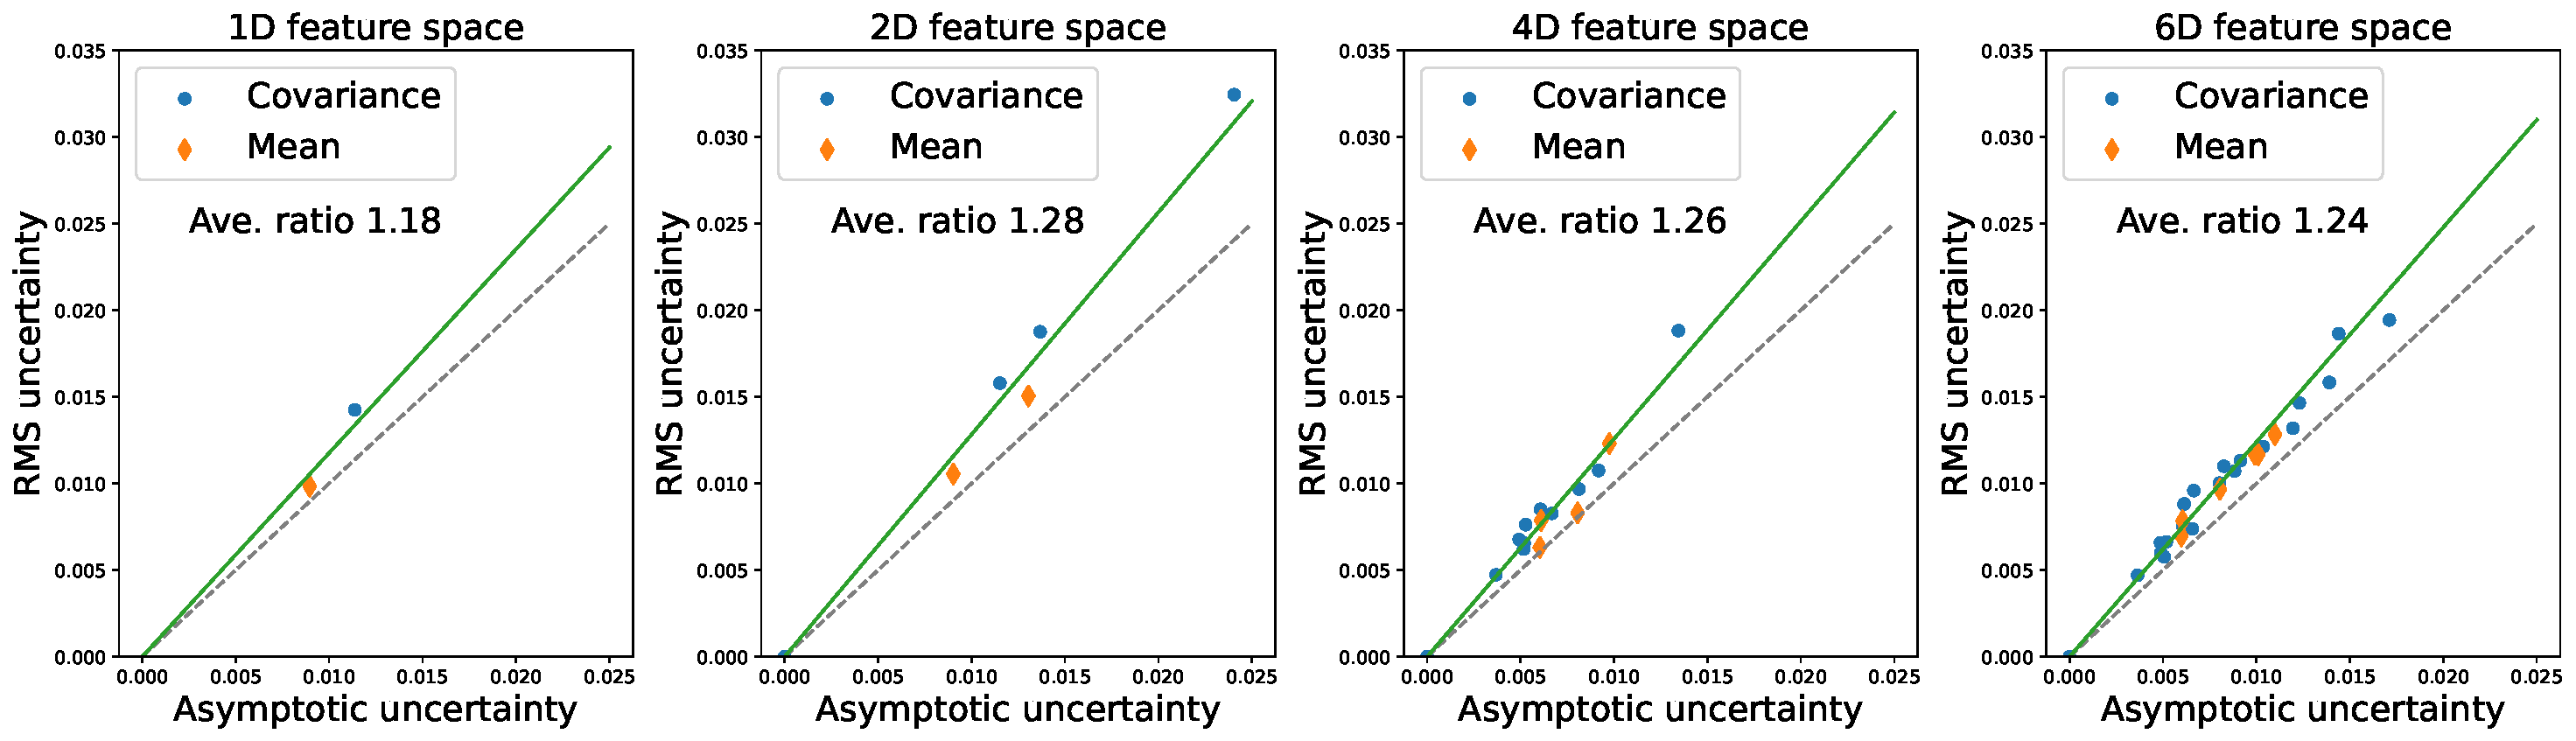
\includegraphics[width=\linewidth]{figures/chapter-07/nn-uncertainties-vs-nd.pdf}
    \caption[Validation of asymptotic uncertainty estimates across dimensionalities in unbinned unfolding.]{Comparison of empirical root-mean-square (RMS) parameter uncertainties with mean asymptotic uncertainty estimates for all model parameters across \(d = 1, 2, 4, 6\) unbinned unfolding studies. Each point represents a single parameter (mean or covariance matrix element) from the multivariate Gaussian models.
    %
    The blue circles denote components of the mean, and the orange diamonds denote components of the covariance.
    %
    The grey dashed line indicates perfect agreement (unit slope), while the green solid line shows the least squares fit for each dimensionality, with slope equal to the mean RMS/asymptotic ratio. 
    %
    The systematic deviation above the unit line demonstrates that asymptotic uncertainties consistently underestimate the true parameter uncertainties, with the underestimation factor increasing from approximately 1.05 in \(d = 1\) to 1.25 in \(d = 6\).
    %
    This trend reflects the growing impact of finite sample effects and parameter correlations in higher dimensions, where the Fisher information matrix becomes less accurate. 
    %
    The increasing scatter with dimensionality indicates heterogeneous behaviour across different parameter types, with off diagonal correlation parameters typically showing larger deviations than mean parameters.\footnotemark}
    \label{fig:rms-asy-dim}
\end{figure}
\footnotetext{Figure create by Owen Long~\cite{Desai:2025mpy}.}
            For every fit parameter, that is, all $\mu_k$ and all unique $\sigma^2_{kl}$, compute the empirical RMS is computed over 500 pseudo--experiments, and the average asymptotic error reported by the na\"ive unbinned likelihood Hessian.
            %
            If the likelihood were well calibrated, these two quantities
            should coincide.
            %
            \cref{fig:rms-asy-dim} plots RMS versus asymptotic error for all parameters in \(d \in\qty{1, 2, 4, 6}\).
            %
            The dashed diagonal marks perfect agreement and the solid green line has a slope fixed to the mean of the RMS/asymptotic error ratio for that dimension.
            
            In each case, the RMS uncertainty is higher than the asymptotic uncertainty.
            %
            The ratio of the RMS uncertainty to the asymptotic uncertainty is roughly the same for all of the model parameters with the ratio ranging from \(\numrange{1.18}{1.28}\).
            %
            The analytic error bars understate the true variance by a factor of about \(\numrange{3}{4}\), consistent with the effective sample size argument~\cite{Yang2011EffectiveAnalyses, jones_effective_2021, geyer_introduction_2011}, \textit{vide} \cref{sec:formalism}.
            
            \cref{fig:rms-asy-6D-res} repeats the \(d = 6\) study with detector resolution scaled by $0,1,2,$ and $3$ relative to the $\sigma_{\det}$ in \cref{tab:highD-params}.
            %
            The slope grows with the smearing factor, confirming that weight correlations, not intrinsic variance, drive the failure~\cite{Langenbruch:2019nwe}.

            In high dimensions, the mapped weight vector $w(\mathbf{x})$ is a smooth function on a space where almost all pairs of points are distant.
            %
            Hence the classifier must assign similar gradients to a larger neighbourhood, inflating correlations.
            %
            \cite{rox818_kernel_2025} explains this phenomenon for KDEs, where excessively wide kernels force longer range weight correlations.
            %
            The same effect applies to NNs as well because global normalisation $\sum_i w_i=N_{\text{MC}}$ adds an $\mathcal O(1/N)$ positive correlation to {every} pair of events~\cite{ATLAS:2014ipf}.

            In six dimensions the na\"ive asymptotic formula would underestimate statistical errors for several covariance elements, while the RMS spread shows true uncertainties.
            %
            Either a binned-covariance approach  or a correlation-aware unbinned likelihood~\cite{Adye2017RooUnfoldTh} is necessary.
            %
            Recent proposals such as Schr\"odinger bridge unfolding or low-rank covariance compression~\cite{wu_high-dimensional_2018} offer interesting possibilities for exploration.


\begin{figure}
    \centering
    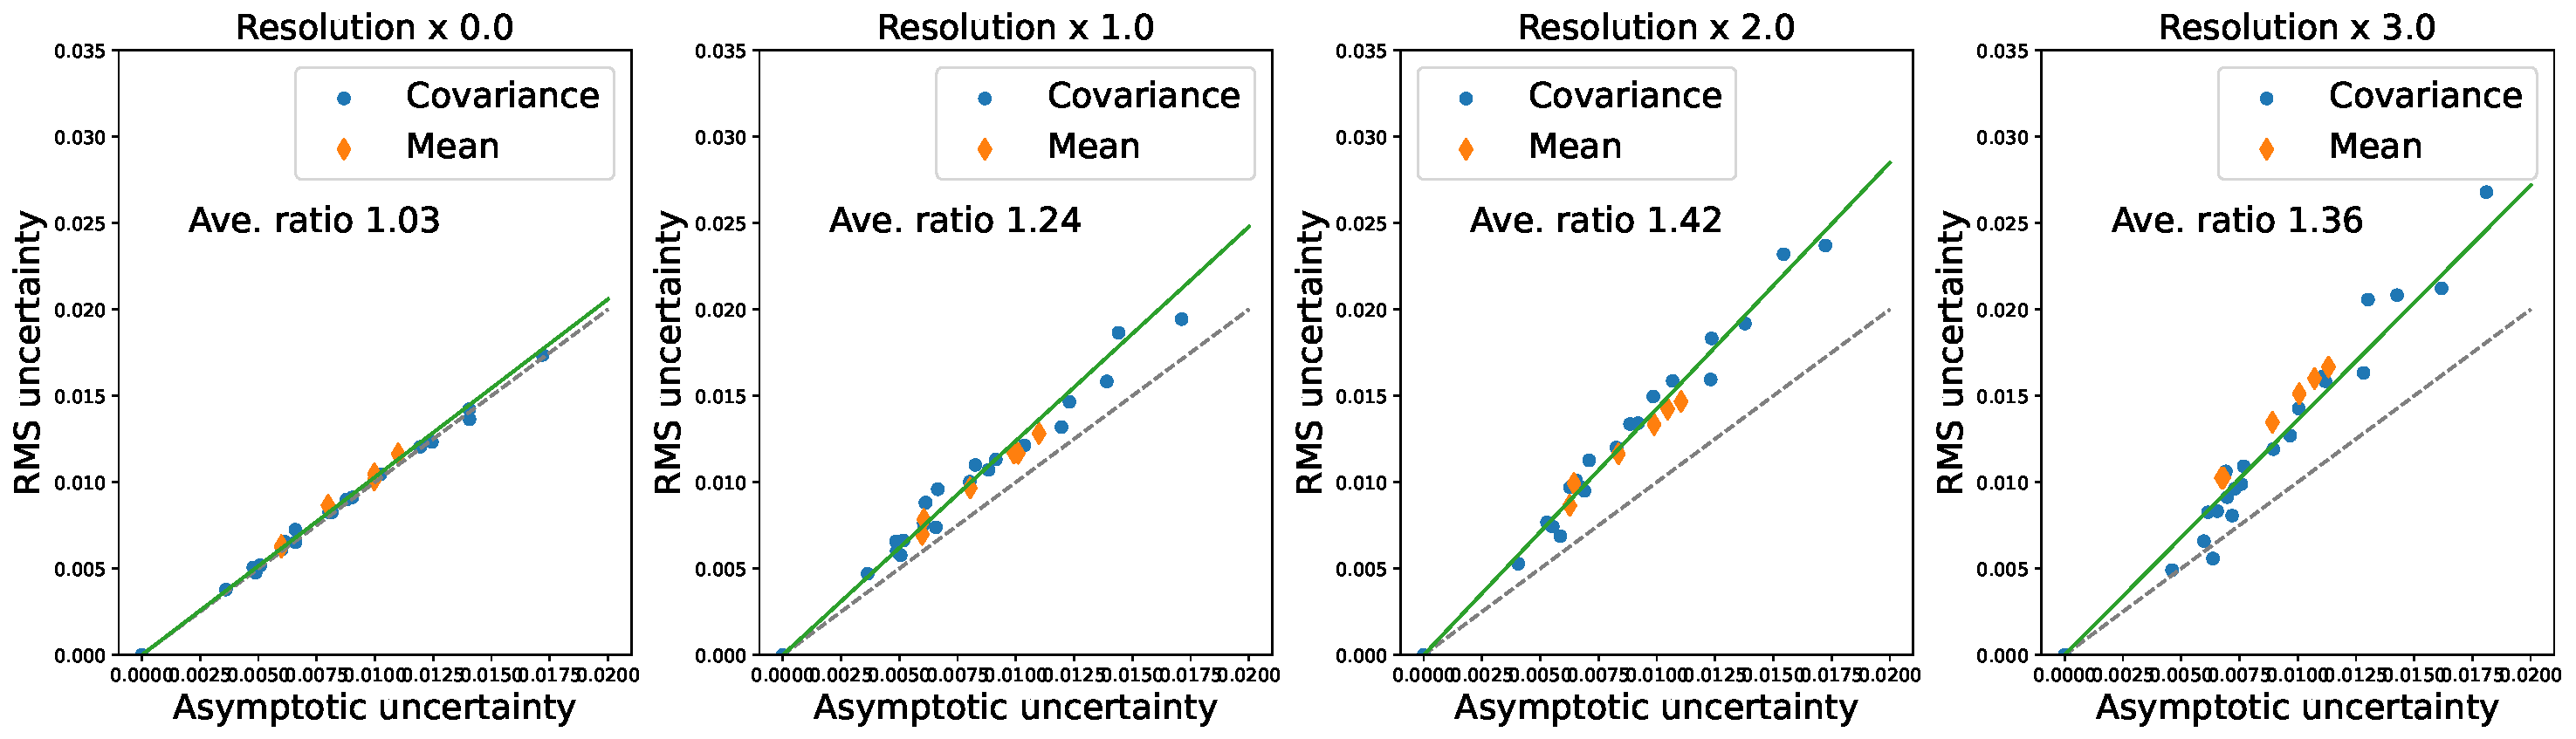
\includegraphics[width=0.8\linewidth]{figures/chapter-07/nn-uncertainties-6d-res-var.pdf}
    \caption[Impact of detector resolution on asymptotic uncertainty reliability in 6-dimensional unfolding.]{Comparison of empirical RMS uncertainties with asymptotic estimates for the six dimensional unfolding study across four detector smearing configurations. The analysis uses smearing scale factors of 0, 1, 2, and 3, where the scale factor multiplies the baseline detector resolution parameters $\boldsymbol{\sigma}_{\text{det}}$ listed in Table~\ref{tab:highD-params}.
    %
    The grey dashed line indicates perfect agreement, while green line shows least squares fits for each smearing level.
    %
    The RMS/asymptotic ratio increases monotonically with detector smearing, from 1.15 at perfect resolution to 1.45 at \(3\times\) smearing, demonstrating that asymptotic uncertainties become increasingly optimistic as detector effects worsen. This degradation arises from increased parameter correlations induced by the unfolding process when compensating for information loss and the breakdown of the local quadratic approximation underlying the Fisher information matrix when the likelihood surface becomes more complex.
    %
    The vertical spread of points also increases with smearing, indicating that the reliability of asymptotic estimates becomes more parameter dependent. Correlation parameters (off-diagonal elements of $\boldsymbol{\rho}$) show particularly poor estimation at high smearing levels, with some parameters exhibiting RMS/asymptotic ratios exceeding 2.0. These findings emphasize that careful uncertainty validation is essential when applying unbinned unfolding to experiments with significant detector effects.\footnotemark
    }
    \label{fig:rms-asy-6D-res}
    \end{figure}
\footnotetext{Figure create by Owen Long~\cite{Desai:2025mpy}.}

\section{Conclusions and outlook.}
    This chapter presented a detailed study of parameter inference performed on an unbinned unfolded dataset, using a controlled Gaussian simulation.
    %
    Employing a simplified scenario where the true distribution and detector response are known analytically facilitates isolating and rigorously examining the statistical subtleties introduced by unbinned unfolding.
    
    The Gaussian studies demonstrated that preserving event level information until the final fit can indeed confer a tangible advantage: an unbinned unfolding followed by binned parameter estimation was observed to outperform a fully binned analysis in terms of fit precision.
    %
    This validates the intuitive principle that one should delay information reductio as much as possible in the analysis chain, thereby maximising the use of available information.
    %
    Importantly, however, the findings also exposed critical caveats that must temper this optimism, especially when interpreting unbinned results with standard inference techniques.

    A central observation is that the output of an unfolding procedure violates the usual assumption of statistical independence among events.
    %
    In these studies, the iterative \textsc{OmniFold} procedure produces a weighted set of ``unfolded'' events that are correlated with one another.
    %
    A na\"ive unbinned likelihood based inference, which treats the unfolded events as if they were independent observations, fails to yield reliable uncertainty estimates.
    %
    In particular, when event--to--event correlations are ignored, the standard asymptotic formulae for parameter uncertainties\footnote{derived from a Fisher information or Hessian approximation} become invalid.
    
    Concretely, the na\"ive application of an unbinned maximum likelihood fit significantly underestimates the true uncertainty on the fitted parameters in Gaussian examples.
    %
    This underestimation was evidenced by comparing the analytic errors to the empirical spread of fit results across many pseudo-=experiments.
    %
    The analytic errors, assuming independence, were significantly smaller than the actual RMS of the fitted parameters.
    
    Such a discrepancy is a direct manifestation of ignoring the induced correlations and a clear warning that conventional unbinned inference tools cannot be directly applied to unbinned unfolded data.
    %
    In short, the lack of statistical independence introduced by unbinned unfolding can invalidate classical error estimates.
    %
    Thus the entire inferential procedure must be handled with care.

    On the positive side, the investigation also highlighted that correlation aware approaches can effectively restore valid inference, albeit with practical limitations.
    %
    When one incorporates the inter--event correlations into the analysis, one finds that the derived uncertainties align with the true performance of the fit.
    %
    In the Gaussian studies, the numerically estimated uncertainties, obtained from the spread of outcomes over many trials, agree well with a covariance informed analytical approach, confirming that the primary cause of the asymptotic formula breakdown was the neglect of correlations.
    %
    This serves as an important proof of principle.
    %
    If one properly accounts for the covariance between events\footnote{or as the case may be, between event weights} in the unbinned dataset, inference methods can yield correct confidence intervals and hypothesis tests even in the unbinned paradigm.
    %
    However, it should also be emphasised that currently available unbinned covariance aware treatments are computationally challenging to scale.
    
    In a binned analysis the covariance matrix is of manageable size, but in an unbinned analysis even if a suitable covariance kernel were developed, one in principle faces an $N \times N$ covariance kernel among $N$ events or event weights, which is intractable for the large event samples typical of HEP data.
    %
    The use of bootstrap ensembles to numerically evaluate uncertainties, while effective for a toy study, is expensive for high dimensional or high multiplicity data.
    %
    Thus, the practical implementation of correlation aware unbinned inference encounters serious scaling limitations, underscoring the need for new strategies to handle or approximate these large covariance structures.

    Crucially, the results presented here should be viewed as a cautionary case study rather than a definitive statement on all unbinned analyses. 
    %
    They were obtained in an idealised Gaussian context, with complete knowledge of the generative process.
    %
    This controlled setup allows one to rigorously identify potential pitfalls and verify proposed solutions, but it also means that the qualitative behaviours observed might not universally translate to real data.
    %
    In particular, the observation that ignoring correlations had little impact on the central values and empirical precision of the fit in the Gaussian example may be a fortunate consequence of the symmetry and simplicity of that example.
    %
    One should not assume this will hold in general.
    
    Therefore, while this study provides a rigorous proof of principle and important warnings, further work is required to generalise of these findings.
    %
    The takeaway is the set of statistical issues that could plausibly afflict unbinned cross section measurements, and the verification of their existence in a controlled setting.
    %
    It now remains to investigate how these issues manifest in realistic analyses.

    Looking ahead, this work motivates several important future directions for both methodology and application.
    %
    An immediate next step is to extend these diagnostic studies to real HEP observables and data.
    %
    It will be invaluable to apply similar techniques (e.g. pseudodata experiments, bootstrap uncertainty evaluations, and covariance measurements) to a realistic experimental unfolding scenario, for example, a differential cross section measurement published with unbinned results, to evaluate the size of event level correlations and to quantify their impact on parameter fits.
    %
    Such studies on real or high fidelity simulated data would confirm whether the cautionary lessons from the Gaussian example are broadly applicable, and could reveal any additional complications arising from more complex data structure or detector effects.
    
    Another critical line of research is to develop new statistical frameworks for unbinned inference that explicitly account for event correlations.
    %
    This could involve formulating modified likelihood functions or test statistics that include correlation terms, or designing hybrid approaches that retain the advantages of unbinned data while imposing an effective covariance model.
    %
    The ultimate goal would be to have an unbinned inference methodology that is correlation aware by construction, obviating the need for \textit{ad hoc} binning or numerical uncertainty estimates.
    
    In tandem with this, there is a clear need for scalable covariance approximation techniques.
    %
    Instead of attempting to handle a full covariance kernel of enormous dimension, one might seek low rank representations, clustering of events into groups with approximate independence, or other dimensionality reduction methods to capture the dominant correlation effects without the full cost.
    %
    Research into such approximations, potentially informed by the machine learning algorithms used in unbinned unfolding, will be essential to make correlation aware inference feasible for large datasets.
    
    Finally, further explorations of the interplay between machine learning regularisation and inference accuracy could be informative.
    %
    A deeper understanding of how the ML aspects affect downstream inference, for instance, whether a stronger regularisation might reduce variance at the cost of introducing bias or correlations, would be extremely valuable.
    %
    By addressing these open questions, the community can build on the foundation laid in this work.

    In summary, this chapter has established a foundational understanding of unbinned inference on correlated data, highlighting both the potential benefits of fully unbinned analyses and the new statistical challenges they pose.
    %
    The Gaussian studies act as a proof of principle, rigorously demonstrating that unbinned unfolding methods can be combined with parameter fits, but also warning that ignoring induced correlations can invalidate conventional uncertainty estimates.
    %
    These conclusions, drawn in a simplified setting, strongly motivate the development of improved tools and methods before applying unbinned inference to precision measurements.
    %
    As the field moves toward ever more complex and high-dimensional data analyses, the insights gained here will guide the creation of a robust statistical framework for unbinned cross section measurements, one that maximizes information usage while properly accounting for the complex correlations introduced by the unfolding process.
    %
    The lessons of this chapter therefore serve as both a caution and a call to action, laying the groundwork for more reliable unbinned inference techniques in high energy physics.
%\chapter{[Optional] Towards Robust Unfolding with Nuisance Parameters}
\begin{itemize}
    \item The challenge of detector response uncertainties
    \item Profiled unfolding methodology
    \item Simultaneous learning of response and physics parameters
    \item Proof-of-concept with gaussians
    \item Applications and limitations
    \item Future development directions [Note: This chapter can be easily removed if paper is not completed]
\end{itemize}
\chapter{Symmetries in data: connections to unfolding challenges.}
\label{chap:symmetrygan}

\section{Symmetries and unfolding.}
    \subsection{The complementary nature of symmetry discovery and unfolding.}
        Unfolding, as discussed, refers to the inverse problem of inferring underlying truth level distributions from observed detector level data, accounting for distortions due to limited resolution and acceptance.
        %
        Symmetry discovery, aims to identify invariant transformations of the data, that is to say, operations under which the probability distribution of the dataset remains unchanged in a statistical sense~\cite{shaw_lie_2025, shaw_symmetry_2024, hagemeyer_learning_2022}.
        
        At first glance, these two tasks appear distinct;
        %
        one concerns recovering numerical distributions, while the other uncovers structural invariances.
        %
        However, symmetry discovery and unfolding are in fact complementary facets of data driven inference, and integrating the two can yield deeper insights and improved measurements.
    
        From a conceptual standpoint, both tasks share the common goal of revealing hidden truth from observed data.
        %
        Unfolding endeavours to remove the ``detector mask'' and recover the true differential cross section or underlying distribution that generated the measurements.
        %
        Symmetry discovery seeks to reveal underlying structures or invariances in the data---patterns that persist under transformations, reflecting fundamental symmetries of the physical process or the measurement apparatus.
    
        In practice, these goals can be intertwined.
        %
        If one discovers a symmetry in the dataset, that knowledge can constrain the unfolding procedure by reducing the effective degrees of freedom in the solution space.
        %
        Conversely, a properly unfolded distribution is expected to manifest latent symmetries that may have been obscured by detector effects in the raw data.
        %
        Thus, identifying a symmetry and unfolding a distribution reinforce one another.
        %
        The former provides a guiding principle or constraint for the latter, while the latter provides a cleaner canvas on which the former can be observed.
    
        Imposing a symmetry as a prior constraint in unfolding can be seen as a form of physically motivated regularisation.
        %
        For example, architectures that conserve four--momentum or enforce Lorentz invariance by design, as discussed in \cref{chap:ml-for-unfolding}, effectively impose such constraints, narrowing the set of viable solutions.
        %
        By restricting solutions to those that respect a discovered or expected invariance, one reduces the space of admissible unfolded distributions to those that are physically plausible, which leads to improved stability and fidelity of the results~\cite{Brehmer:2024yqw}.
    
        This principle has been implicitly utilised in classical unfolding and simulation based calibration.
        %
        For example, one could assume certain symmetries such as isotropy or detector uniformity when designing the response matrix or when combining symmetric regions of phase space to reduce uncertainties.
        %
        With a data driven symmetry discovery tool in hand, one need not rely solely on presumed symmetries.
        %
        Instead, one can verify them empirically or even discover unexpected invariances.
        %
        In turn, these empirically verified symmetries can be fed back into the inference pipeline to sharpen measurements, such that a discovered symmetry can inform the unfolding algorithm so that the final measured distribution upholds the invariance.
    
        It is instructive to compare symmetry discovery and unfolding side by side to appreciate their complementary roles.
        %
        \cref{tab:unfolding_vs_symmetry} summarises the differences and points of contact between the two.
    
        While unfolding typically requires an explicit model of the measurement process\footnote{E.g., a response matrix or a parametrised detector simulation.} and often relies on supervised learning or iterative inversion techniques, symmetry discovery can be pursued in an unsupervised manner, requiring only the dataset and a class of transformations to probe.
        %
        The outcome of unfolding is a corrected distribution intended for direct physical interpretation.
        %
        The outcome of symmetry discovery is a characterisation of invariances, a set of transformations $T$ such that the dataset’s distribution is invariant under $T$ within statistical uncertainties.
        %
        These outcomes are different in nature, but they are mutually beneficial.
    
        Knowledge of invariant structure can guide numerical inference, and conversely, obtaining a more accurate numerical distribution makes it easier to discern subtle invariant patterns.
        %
        In essence, symmetry discovery and unfolding can form a feedback loop in the broader endeavour of measurement and inference, where each can improve the other.
\begin{table}
    \centering
    \caption[Comparative analysis of unfolding and symmetry discovery methods in particle physics.]{Comparison of unfolding and symmetry discovery approaches in high-energy physics data analysis. While unfolding aims to correct detector effects to recover true physical distributions, symmetry discovery seeks to identify invariance properties directly from data. These complementary techniques can be combined synergistically: unfolding provides cleaner distributions where symmetries become more apparent, while discovered symmetries can constrain and regularise the unfolding process. This bidirectional relationship enables more robust extraction of physical information from experimental data, particularly in scenarios where detector effects might obscure underlying symmetries or where symmetry constraints can help resolve unfolding ambiguities.}
    \label{tab:unfolding_vs_symmetry}
    \begin{tabular}{@{}p{0.12\linewidth} p{0.41\linewidth} p{0.41\linewidth}@{}}
        \toprule
        \textbf{Aspect} & \textbf{Unfolding} & \textbf{Symmetry discovery} \\
        \midrule
        \textbf{Primary goal} & 
        Reconstruct true distributions from detector level observations by inverting detector response & 
        Identify transformation groups under which distributions remain invariant \\
        \midrule
        \textbf{Inputs} & 
        \begin{tabular}[t]{@{}l@{}}
        • Measured detector level data\\
        • Detector response matrix or\\
        • Regularisation scheme
        \end{tabular} & 
        \begin{tabular}[t]{@{}l@{}}
        • Measured or unfolded data\\
        • Parametrised transformations\\
        • Invariance test statistics
        \end{tabular} \\
        \midrule
        \textbf{Outputs} & 
        \begin{tabular}[t]{@{}l@{}}
        • Differential cross sections\\
        • Probability density functions\\
        • Uncertainties/correlations
        \end{tabular} & 
        \begin{tabular}[t]{@{}l@{}}
        • Symmetry generators/parameters\\
        • Invariance confidence levels\\
        • Conserved quantities
        \end{tabular} \\
        \midrule
        \textbf{Basis} & 
        Incorporates domain knowledge through priors/constraints to regularise ill posed inverse problem & 
        Tests generic transformation classes allowing data driven discovery of invariances \\
        \midrule
        \textbf{Approach} & 
        Statistical inference problem to invert \(p(x) =\int r(x\mid z)\,p(z)\,\dd z\) & 
        Hypothesis testing framework to evaluate $p({x}) \stackrel{?}{=} p(g({x}))\cdot|g'(x)|$ \\
        \midrule
        \textbf{Benefit} & 
        Produces distributions where true physical symmetries manifest more clearly, enabling validation of theoretical predictions and discovery of emergent invariances & 
        Discovered symmetries constrain unfolding solution space, reducing regularisation dependence and 
improving stability of deconvolution \\
        \bottomrule
    \end{tabular}
\end{table}
    \subsection{Symmetry aware cross sections.}
        Since differential cross section measurements lie at the core of particle physics,
        %
        achieving high precision in these measurements is essential, as even subtle deviations between the measured spectra and theory predictions can signal new physics or the need for refined models.
        %
        In this context, symmetries play a pivotal role in both the design and interpretation of cross section measurements.

        Many physical processes come with known symmetry expectations.
        %
        For instance, in proton--proton collisions producing particle jets, one expects azimuthal symmetry about the beam axis, i.e. the physics is invariant under rotations in the plane perpendicular to the beam.
        %
        Consequently, the differential cross section should, after correcting for detector non-uniformities, be independent of the absolute azimuthal angle $\phi$ of a jet or dijet system~\cite{Chen:2025rjc, Spinner:2025prg, Pedersen:2023fgr, Froidevaux2009ExperimentalCollider}.
        
        Likewise, for processes initiated by identical colliding particles, one often anticipates a symmetry between forward and backward directions.
        %
        In a symmetric proton--proton collider, this implies that the rapidity distribution of a centrally produced system \footnote{E.g., dijet pair.} should be symmetric about zero rapidity~\cite{Cheung:2017loo, CMS:2011xqa, Cotogno:2020iio}.
        %
        Such symmetry means that the cross section for producing a system at rapidity $+y$ is the same as at $-y$, all else being equal.
        %
        If a measured differential cross section exhibits a significant asymmetry in these variables after unfolding and acceptance corrections, it would either indicate a previously unaccounted detector bias or hint at a physical effect, both of which are of interest to investigate.

        Being symmetry aware in a measurement can mean two things.
        %
        First, verifying that expected symmetries are indeed present, within uncertainties, in the data, and second, leveraging those symmetries to improve the measurement.
        %
        On the verification side, symmetry considerations provide valuable consistency checks.
        %
        Experiments can test whether their unfolded distributions respect fundamental symmetries, and a failure to observe an expected symmetry is a red flag, prompting scrutiny of systematic effects or potential new physics contributions.

        On the other hand, when a symmetry is confirmed, one can exploit it to gain statistical and systematic advantages.
        %
        For example, if a distribution is believed to be symmetric in a certain variable, one can ``augment" or combine data from symmetric regions, effectively doubling the effective statistics for that distribution.
        %
        A common practice is to report differential cross sections as a function of $|y|$ or other symmetry reduced variables, which assumes $y \leftrightarrow -y$ symmetry and thereby reduces statistical fluctuations~\cite{CMS:2013zfg, ATLAS:2014rjv, ATLAS:2016vlf}.
        %
        By incorporating symmetry in this manner, uncertainties can be reduced and the measurement becomes more robust against localised fluctuations.

        Symmetry aware analysis also serves to impose physically motivated constraints that guard against overfitting noise in the unfolding process.
        %
        If one has discovered that a distribution must be invariant under a transformation,\footnote{E.g., rotating the entire event by some angle, or exchanging two identical particles in the final state.} imposing this invariance in the unfolding procedure will tie neural network parameters or bin values together that would otherwise float independently.
        %
        This effectively decreases the number of free parameters describing the unfolded result, acting as a regulariser that prefers solutions consistent with the symmetry.
        %
        The net effect is an improvement in the precision of the measured cross section and a reduction in spurious oscillatory features that might arise from statistical fluctuations.
        %
        Moreover, by reducing the dependence on bins with low occupancy (because they are combined with their symmetric counterparts), binned symmetry aware unfolding can also mitigate the impact of detector acceptance edges or inefficiencies in specific regions of phase space.

        It is important to note, however, that any symmetry based constraint should be applied with careful consideration. One must ensure that the symmetry is either theoretically well founded or empirically validated, lest one impose a false invariance and obscure a genuine asymmetry.
        %
        This caution further motivates the need for data driven symmetry discovery and validation tools.
        
        One can use methods like \textsc{SymmetryGAN}~\cite{PhysRevD.105.096031} to verify whether the data uphold the symmetry to a high degree of confidence.
        %
        Only then would one proceed to incorporate that symmetry into the unfolding process or in the presentation of results.
        %
        Thus symmetry aware differential cross section measurements can harness known, or discovered invariances to enhance precision and reliability, while simultaneously providing a framework to detect symmetry violations that could point to new phenomena.
    
    The research presented in this chapter builds upon the foundations laid in earlier chapters of this thesis, extending the paradigm of symmetry utilization in the context of measurement and unfolding.
    %
    \cref{chap:theoretical-foundations}, in its survey of existing techniques, provides a statistical foundation for incorporating known symmetries into data analyses.
    %
    It also highlights the challenges such approaches face, such as the need for careful validation of assumptions.
    %
    \cref{chap:ml-for-unfolding} includes references to how \textit{a priori} known symmetries can be hard coded into machine learning models, introducing Lorentz group equivariant networks that guarantee Lorentz invariance in the unfolding of particle physics data~\cite{Bogatskiy:2020tje}.
    %
    The inclusion of symmetry constraints in unfolding models described in \cref{chap:npu,chap:moment-unfolding,chap:ran} through preserving physical invariants like momentum or charge conservation in the generative model would reduce the solution space and lead to more physically plausible unfolded results.
    
    All of these strategies rely on prior knowledge of the symmetry.
    %
    This chapter shifts to an data driven approach that provides a novel, flexible, and fully differentiable deep learning based method to discover symmetries directly from data using adversarial learning, which then might allow one to leverage those discovered symmetries to inform the unfolding process.
    %
    This perspective emphasises the overarching theme of the thesis, the interplay of measurement and inference, by using data driven insights in the form of symmetry discovery to enhance the core measurement task of differential cross section unfolding.

    The remainder of this chapter is organised as follows.
    %
    \cref{sec:formalism-and-role, sec:statistical-def-of-symmetries} introduce the formal statistical definition of a dataset symmetry, addressing subtleties like Jacobian volume effects via the concept of an inertial reference density.
    %
    THey also provides a brief overview of the symmetries most relevant to HEP.
    %
    \cref{sec:symmetry-gan-main} presents the \textsc{SymmetryGAN} framework, which employs a generative adversarial network to automatically learn symmetry transformations from data.
    %
    \cref{sec:empirical-experiments} validates this approach on illustrative examples and then applies \textsc{SymmetryGAN} to simulated dijet events, demonstrating how it can uncover physically meaningful symmetries in collider data.
    %
    \cref{sec:symmetry-informed-unfolding} discusses how the discovered symmetry information can be used to constrain unfolding problems: we outline methods to incorporate symmetry constraints into the unfolding procedure to reduce uncertainties and bias.
    %
    In \cref{sec:improved-measurement-prediction}, the chapter introduces a symmetry aware unfolding methodology and discusses how enforcing the symmetries identified by \textsc{SymmetryGAN} can improve the precision of differential cross section measurements.
    %
    Finally, the chapter concludes by highlighting how the insights gained here connect back to the broader narrative of the thesis, reinforcing the benefits of combining machine learning driven discovery with principled measurement techniques.
\section{Formalism and Importance}
\label{sec:formalism-and-role}
    In physics and statistics, a symmetry refers to an invariance of a system or dataset under a well-defined transformation.
    %
    Formally, let $G$ be a group of transformations (continuous or discrete) acting on a space of states or observations $X$.
    %
    A physical system or probability distribution is symmetric under $G$ if applying any transformation $g \in G$ leaves the relevant observables unchanged.
    %
    In group theoretic terms, there exists an action $g: x \mapsto g(x)$ such that for all $x \in X$ and $g \in G$, the value of an function $f(x)$ remains equal to $f(g(x))$.
    %
    However, if $p(x)$ denotes a probability density on $X$, a group $G$ is a symmetry of \(p\) if
    \[
        \forall g \in G \; p(x) \; \dd x = p(g(x)) \; \dd(g(x)).
    \]
    In measure theoretic language, a symmetry corresponds to an invariant measure.
    %
    For any measurable subset $A \subseteq X$ and any transformation $g\in F$, \(g\) is a symmetry of \(A\) if $\mu(A) = \mu(g\cdot A)$, meaning the measure assigned to outcomes in $A$ is the same as that for the transformed set $g\cdot A$.
    %
    This definition encompasses both continuous symmetries\footnote{Lie groups, such as rotations depending on a continuous angle parameter.} and discrete symmetries \footnote{groups constructed as Jordan--H\"older extensions~\cite{solomon_brief_2001, HolderDieOrdnungszahlen, jordan_traite_nodate} e.g. a mirror reflection or a permutation of identical objects}.
    %
    Symmetry principles lie at the heart of modern particle physics and also strongly influence experimental measurements.
    %
    At the theoretical level, fundamental symmetries constrain the form of physical laws and often correspond to conserved quantities or selection rules.
    %
    At the data level, symmetries, and their breaking, shape the distributions of observed events and can be leveraged for more efficient data analysis.
    %
    In the context of colliders, many observables are governed by symmetries of the underlying theory as well as symmetries introduced by the detector and measurement process.
    %
    It is therefore crucial to articulate how these symmetries operate both in ideal physics scenarios and in real observations.
    %
    This section provides a rigorous overview of symmetries relevant to collider physics and measurements.
    %
    It begins with the fundamental symmetries in particle physics that underlie observable phenomena in \cref{subsec:hep-symmetries}.
    %
    \cref{subsec:detector-symmetries} discusses symmetries in detector response functions and how the measurement apparatus can preserve or violate underlying invariances.
    %
    Next, \cref{subsec:cross-section-symmetries} examines how symmetries manifest in measured cross sections and data distributions, clarifying the translation from physical symmetry to statistical patterns in experimental histograms.
    %
    Finally, \cref{subsec:noisy-symmetries} highlights the challenges in identifying symmetries from noisy data, setting the stage for data--driven symmetry discovery techniques.
    %
    This foundation will be essential for later sections that introduce methods like \textsc{SymmetryGAN} for learning symmetries from data.

    \subsection{Fundamental symmetries in HEP.}
    \label{subsec:hep-symmetries}
        Particle physics is built upon a framework of symmetries that determine the allowed forms of interactions and the conservation laws observed in experiments.
        %
        Spacetime symmetries, in particular subgroups of the Poincar\'e group, are foundational.
        %
        The Poincar\'e group includes continuous Lorentz invariance (rotations and boosts) and translations (in spacetime).
        %
        Lorentz invariance implies that the laws of physics take the same form in any inertial reference frame.
        %
        Equivalently, physical observables can be expressed in terms of Lorentz invariant quantities\footnote{E.g., invariant masses, angles, and dimensionless ratios.} that remain unchanged under boosts or rotations.
        %
        For example, the Mandelstam variables $s$, $t$, $u$ in a scattering process or the decay angle distribution in a particle's rest frame are formulated to respect Lorentz symmetry.
        %
        In practice, exact Lorentz invariance means there is no preferred direction or absolute velocity in the underlying theory.
        %
        A given interaction process should yield identical outcomes whether the laboratory frame is, say, Earth bound or boosted to a constant velocity.
        %
        As a consequence of Lorentz symmetry and spatial isotropy, angular momentum and linear momentum are conserved in isolated systems\footnote{Noether’s theorem associates these conservations with rotational and translational symmetry, respectively~\cite{noauthor_nachrichten_nodate}}.
        %
        Time translation symmetry leads to energy conservation, ensuring that system's total energy and the collision centre of mass energy are fixed constants of motion.
        %
        These spacetime symmetries are exact symmetries of all known fundamental interactions and provide the basis for defining covariant formalisms in quantum field theory.

        Beyond spacetime, the internal symmetries of the Standard Model dictate the spectrum of particles and their interactions.
        %
        Chief among these is the gauge symmetry group $SU(3)_C \times SU(2)_L \times U(1)_Y$, which defines quantum chromodynamics and electroweak theory.
        %
        Gauge symmetries are local symmetries that require the introduction of gauge bosons;
        %
        although these are internal symmetries rather than symmetries of observable spacetime, they have observable consequences such as electric charge conservation, associated with $U(1)_Y$ hypercharge symmetry, and the existence of multiple particle generations.
        %
        The gauge symmetries of the Standard Model are spontaneously broken in certain cases.\footnote{One of the most notable examples is the electroweak $SU(2)_L \times U(1)Y$ breaking to $U(1)_{\text{EM}}$ via the Higgs mechanism, which introduces masses for the $W^\pm$ and $Z$ bosons and differentiates the electromagnetic and weak interactions.}
        %
        However, even broken symmetries leave remnant effects, such as the custodial symmetry in the Higgs sector or approximate conservation of isospin in QCD.
        %
        These internal symmetries set selection rules.
        %
        Processes that violate gauge charge conservation are forbidden and decays proceed only via symmetric channels.

        Alongside continuous symmetries, several discrete symmetries play a crucial role in particle physics.
        %
        The most prominent are C (charge conjugation, exchanging particles with their antiparticles), P (parity, spatial inversion or mirror reflection), and T (time reversal).
        %
        Each of these can be considered a transformation that might leave the fundamental laws invariant.
        %
        In the Standard Model, CP symmetry is approximately a symmetry of electromagnetic and strong interactions, but notably broken in weak interactions.
        %
        This manifests as differences in the behaviour of matter and antimatter.
        %
        Like most notable instance of this is the well known CP violation in neutral kaon and $B$-meson decays means those processes occur at different rates or with different phase relationships than their CP-mirrored counterparts~\cite{Neubert:1996qg}.
        %
        If CP were an exact symmetry of the dynamics, one would expect, for example, the angular distribution of decay products in a mirror--reflected process, swapping particles for antiparticles, to be identical to the original.
        %
        The observed deviations are vital clues to physics beyond simple symmetries.
        %
        Parity by itself is also violated maximally in the weak interaction.\footnote{ classic examples are the left handed nature of neutrinos and the parity asymmetric angular distribution of electrons in polarized $^{60}$Co beta decay~\cite{Wu:1957my}}
        %
        On the other hand, the strong and electromagnetic interactions conserve parity, so for many processes, especially at high energies where electroweak effects are subdominant, it is a good symmetry.
        %
        A process governed by QCD, like multijet production, should occur equally in a configuration and its mirror reflected image, unless the experimental setup selects a handedness.
        %
        Charge conjugation is likewise not a symmetry of the full Standard Model, since, for example, there are no right handed neutrinos to pair with left handed ones under C, but for purely electromagnetic processes C symmetry implies, that producing a negatively charged particle is as likely as producing the corresponding positively charged antiparticle under equivalent conditions.
        
        Importantly, the combination CPT is believed to be an exact symmetry of local quantum field theory.
        %
        CPT symmetry implies, for instance, that particle and antiparticle masses and lifetimes are exactly equal~\cite{Kostelecky:1998ic}.
        %
        While CPT is typically not directly tested by single distribution symmetries in HEP experiments, it provides a fundamental consistency check on any observed CP or T violation. \cref{tab:fundSymSummary} summarises these fundamental symmetries, their group theoretic character, and their status in the Standard Model.
\begin{landscape}
\begin{longtable}{@{}m{0.13\linewidth} M M m{0.24\linewidth} m{0.16\linewidth}@{}}
    \caption[Fundamental symmetries and their manifestations in HEP observables.]{Summary of fundamental symmetries relevant to particle physics, their group theoretic structure, and experimental signatures. The table includes spacetime symmetries, gauge symmetries, discrete symmetries, and quantum statistical symmetries.
    %
    ``Conserved charge'' refers broadly to conserved quantities arising from continuous symmetries via Noether's theorem or to quantum numbers constrained by discrete symmetries.
    %
    The ``Status in SM'' column indicates whether each symmetry is exact, approximate, or explicitly broken within the Standard Model.
    %
    Observable signatures provide experimental handles for testing these symmetries.
    %
    The hierarchy of symmetry breaking guides the search for BSM physics through precision tests of invariance.}
    \label{tab:fundSymSummary} \\
    \toprule
    \textbf{Symmetry} & \textbf{Group structure} & \textbf{Conserved charge} & \textbf{Observable signatures} & \textbf{Status in SM} \\
    \midrule
    \endfirsthead
    
    \multicolumn{5}{c}{\textit{Table \ref{tab:fundSymSummary} continued from previous page}} \\
    \toprule
        \textbf{Symmetry} & \textbf{Group structure} & \textbf{Conserved charge} & \textbf{Observable signatures} & \textbf{Status in SM} \\
    \midrule
    \endhead
    
    \midrule
    \multicolumn{5}{r}{\textit{Continued on next page}} \\
    \endfoot
    
    \bottomrule
    \endlastfoot
    
    \textbf{Lorentz}\-\textbf{invariance} & 
    \mathrm{SO}(3,1) & 
    x^\mu p^\nu - x^\nu p^\mu & 
    Invariant mass; angular distributions & 
    Exact~\cite{Kostelecky:2010ze} \\
    \midrule
    \textbf{Spacetime translation} & 
    \mathbb{R}^{1,3} & 
    p^\mu & 
    Missing momentum; vertex momentum conservation & 
    Exact~\cite{Weinberg:1995mt} \\
    \midrule
    \textbf{Gauge\-symmetry} & 
    \mqty*{
    SU(3)_C\times\\
    SU(2)_L\times U(1)_Y} & 
    \mqty*{\text{Colour, isospin,}\\\text{hypercharge}} & 
    Jet colour flow patterns; $W$ boson charge asymmetry; & 
    Exact (local)~\cite{peskin_introduction_1995} \\
    \midrule
    \textbf{Electroweak} & 
    \langle H \rangle \neq 0 & 
    M_W, M_Z & 
    $\rho = M_W^2/(M_Z^2\cos^2\theta_W)$ & 
    Broken~\cite{PhysRevLett.13.508} \\
    \midrule
    \textbf{Charge conjugation (C)} & 
    \mathbb{Z}_2: \psi \to \mathcal{C}\bar{\psi}^T & 
    \alpha_{q\pm}\leftrightarrow\alpha_{\bar{q}\mp} & 
    $e^+/e^-$ production ratios; $\pi^0 \to \gamma\gamma$, $\pi^0 \not\to 3\gamma$ & 
    Conserved in QED/QCD; violated in weak~\cite{Wu:1957my} \\
    \midrule
    \textbf{Parity (P)} & 
    \mathbb{Z}_2$: $\vec{x} \to -\vec{x} & 
    \eta_P = \pm 1 & 
    Neutrino helicity; asymmetric $\beta$ decay & 
    Conserved in QED/QCD; violated in weak~\cite{Lee:1956qn} \\
    \midrule
    \textbf{CP} & 
    \mathbb{Z}_2 \times \mathbb{Z}_2 & 
    \delta_{CP}, \theta_{\text{strong CP}} & 
    $B^0$-$\bar{B}^0$ mixing asymmetry; kaon decay: $\epsilon_K \sim 10^{-3}$ & 
    Violated: $\delta_{CP} \approx 68\deg$~\cite{Charles2005CPFactories} \\
    \midrule
    \textbf{Time reversal (T)} & 
    \mathbb{Z}_2: t \to -t & 
    \text{Amplitudes} & 
    Electric dipole moments; $K_L \to \pi^+ \pi^- e^+ e^-$ decay & 
    Violated (CPT theorem)~\cite{Luders:1957zz} \\
    \midrule
    \textbf{CPT} & 
    \mathbb{Z}_2 \text{ (anti-unitary)} & 
    m, \tau_{q\pm} = m, \tau_{\bar{q}\mp} & 
    $|m_p - m_{\bar{p}}|/m_p < 10^{-10}$; $|\tau_\mu - \tau_{\bar{\mu}}|/\tau_\mu < 10^{-5}$ & 
    Exact (theorem)~\cite{Streater:1989vi} \\
    \midrule
    \textbf{Permutation} & 
    S_n/A_n & 
    \text{Bose/Fermi stats} & 
    HBT correlations in $\pi^+\pi^+$; Pauli exclusion in spectra & 
    Exact~\cite{Pauli:1940zz} \\
\end{longtable}
\end{landscape}

        Beyond the Standard Model’s built in symmetries, there are approximate global symmetries that often prove useful in particle physics.
        %
        Examples include isospin symmetry, an $SU(2)$ symmetry treating up and down quarks as identical in the limit of equal masses, and flavour symmetries, like the $SU(3)$ of the light $uds$ quarks, both of which are not exact, but underlie patterns in hadron production and decay.
        %
        For instance, isospin symmetry implies that processes differing only by swapping an up quark with a down quark, such as producing a proton versus a neutron, have nearly equal cross sections, up to corrections from the up--down mass difference or electromagnetic effects.
        
        Similarly, the universality of physical laws under interchange of identical particles leads to permutation symmetry.
        %
        If two particles of the same type appear in a final state, the probability distribution is invariant under exchanging them.
        %
        In quantum theories this is enforced by (anti)symmetrization of identical particle states.
            %
            In HEP observables, permutation symmetry means that one cannot physically distinguish, say, which of two identical jets in an event is `jet 1' or `jet 2'---any labelling is arbitrary and the underlying physics treats the two jets on equal footing.
            %
            When calculating cross sections, this symmetry is accounted for by dividing by the a symmetry factor to avoid over counting identical configurations.
            
            In practical analyses analysis one often has to impose an ordering, such as `leading' and `subleading' jet by momentum, for convenience, but the fundamental permutation invariance implies that any physical conclusion should not depend on this arbitrary ordering.

            In summary, fundamental symmetries, Poincar\'e (Lorentz and translations), gauge invariances, discrete symmetries like CPT, and permutation invariance for identical particles, provide a set of invariance principles for particle interactions.
            %
            These symmetries constrain the form of theoretical cross sections and transition rates.
            
            Many measurable quantities in experiments such as cross sections, angular distributions, etc., either reflect these symmetries, when they hold, or provide avenues to detect symmetry breaking when deviations are observed.
            %
            However, the symmetries of nature at the fundamental level are not always manifest in what detectors actually record.
            %
            We next turn to how the detector response and measurement process can modify or obscure these symmetries.

    \subsection{Symmetries in detector response functions}
    \label{subsec:detector-symmetries}
        The detector response function $r(x\mid z)$ describes the probability of observing a measurement outcome $x$ given a true state $z$.
        %
        An ideal detector with perfect resolution would preserve all physical symmetries present at the particle level.
        %
        In reality, detectors often break or reduce symmetries that the underlying physics possesses.
        %
        Understanding which symmetries are preserved, approximated, or lost convolution with $r(x\mid z)$ is crucial for interpreting measured data.
        %
        Here we discuss several common invariances and how they are affected by realistic detectors in their response.

        \subsubsection{Spatial uniformity and rotational symmetry.}
            Many detectors are designed with a roughly cylindrical geometry around a natural axis, such as the beam axis in collider experiments, aiming for azimuthal symmetry.
            %
            Hence they are designed to provide close to uniform coverage in the plane normal to the axis.
            
            Ideally, if the physical process yields a uniform distribution in the azimuthal angle $\phi$ (i.e. no preferred direction around the axial line), a perfectly symmetric detector would register an equal number of events in each azimuthal segment.
            %
            In practice, certain asymmetries are present in any measurement.
            
            For example, a detector may have support structures or cabling at certain angles, or irregular segmentation, leading to variation in efficiency with $\phi$.
            %
            The electromagnetic calorimeter (ECAL), as an illustration, might be segmented into modules that cover specific $\phi$ slices.
            %
            Given this, events falling into the gap between modules could be recorded with lower efficiency or energy resolution, creating a $\phi-$dependence in the observed data even if the true distribution was uniform.
            %
            Detectors often have periodic segmentation, meaning continuous rotational invariance is broken down to a discrete rotation symmetry, invariant only under rotations corresponding to full module spacings.
            
            As a concrete example, imagine a detector with 360 identical modules each covering $\Delta\phi = 1^\circ$.
            %
            This detector is invariant under rotation by multiples of \(1\deg\) increments, but a rotation by an arbitrary angle (say $0.5\deg$) would lead to a different alignment of a particle's trajectory with respect to module boundaries, yielding a measurably different response~\cite{Nabat:2024nce}.
            %
            Thus, the continuous symmetry is reduced to a discrete one, and even that discrete symmetry may be imperfect if modules are not exactly identical or have time varying efficiency.
            
            Thus azimuthal symmetry at the physics level is usually preserved approximately by detector design, but slight non-uniformities in $\phi$ response are common and must be accounted for either via calibration or acceptance corrections.

        \subsubsection{Polar coverage and boost invariance.}
            Often detectors in HEP experiments, especially collider experiments, also have limited coverage in the polar direction, along the beam axis.
            %
            No real detector covers the full $4\pi$ solid angle;
            %
            there is always a cut off at some polar angle (or pseudorange $\eta$) beyond which particles escape detection.
            %
            In particular, the forward regions close to a beam are notoriously difficult to instrument.
            
            This breaks the full spherical symmetry of space.
            %
            A process that is symmetric under arbitrary rotations, such as a perfectly isotropic decay in its rest frame, will not appear isotropic in the laboratory measurement if a significant portion of the solid angle is unobserved.
            %
            Detectors are typically ideally symmetric under rotations about the beam axis but not under arbitrary rotations that tilt the beam axis, because the beam direction is a fixed axis of symmetry.
            
            In other words, the presence of beams singles out a preferred direction, the beam axis $\hat{z}$, and detectors are built around this axis. Consequently, the data may reflect cylindrical symmetry, invariant under \(SO(2)\) rotations around $\hat{z}$, but not full $SO(3)$ rotational symmetry.
            
            This also has consequences for Lorentz boost invariance.
            %
            While the underlying physics is Lorentz invariant, the detector is a fixed apparatus in one frame.
            %
            A boost along the beam direction, i.e. a change to the reference frame moving with respect to the collision, will generally change how events are distributed relative to the detector acceptance.
            
            As an example, consider a boost that causes particles to have higher longitudinal momentum;
            %
            in the lab frame, more particles will end up at small polar angles, closer to the beam line, where detection efficiency is lower, thus the observed distribution of, say, pseudorapidity $\eta$ will shift.
            %
            The detector has a finite acceptance in $\eta$, so a Lorentz boost that moves events into the far forward region will result in a fraction of events being lost.
            %
            Therefore, the measured distributions are not invariant under Lorentz boosts, even though the underlying parton level kinematics can be expressed in Lorentz invariant terms.
            
            Thus the physical construction of detectors break global translational and boost symmetry by virtue of being static and having edges.
            %
            A high energy interaction viewed in different inertial frames is physically identical, but a detector at rest in the lab frame will record it differently unless one corrects for acceptance and inefficiencies.

        \subsubsection{Resolution effects and approximate invariance.}
            Even if a symmetry could hold in principle, the resolution and threshold effects of detectors often spoil exact invariance.
            %
            A salient example arises with Lorentz invariance and invariant mass reconstruction.
            
            As a thought experiment, imagine a two body decay producing a pair of muons, such as $Z^0 \to \mu^+\mu^-$.
            %
            The true invariant mass of the muon pair is fixed, irrespective of the $Z$ boson’s momentum, because it is simply a Lorentz scalar.
            %
            However, a detector measures muon momenta with finite precision, and that precision typically degrades at high momentum\footnote{Tracking detectors determine momentum from curvature in a magnetic field, which becomes very small for high momentum muons, leading to larger relative uncertainty in the measurement.}.
            %
            If the $Z$ boson is produced nearly at rest in the lab, its decay muons have moderate momenta and the detector might reconstruct the invariant mass with a narrow resolution.
            %
            If instead the $Z$ is produced with a large boost, the muons each have higher lab frame momenta, and the detector's momentum resolution broadens the reconstructed mass distribution.
            %
            The result is that the distribution of reconstructed $m_{\mu\mu}$ for boosted $Z$ events is broader (and potentially biased) compared to that for non-boosted events.
            
            Thus, a Lorentz boost, which should not matter to an ideal measurement, actually changes the statistical distribution of an observable due to detector response.
            %
            This is an example of an approximately respected symmetry.
            %
            At low boost the symmetry holds well, but at high boost the symmetry is effectively broken by detector effects.
            
            Similarly, thresholds in detector sensitivity (e.g. a calorimeter that only records energy above some minimum) can break symmetry under transformations that redistribute energy.
            %
A detector that is equally efficient for electrons and positrons should demonstrate C symmetry.
%
However, if the process produces a broad energy spectrum, imposing a cut on low energy particles can introduce a bias.
%
Low energy $e^+$ are more likely to be lost than $e^-$ due to their different interaction rates with detector material.
%
In such cases, even an underlying physical symmetry may not yield equal measured counts.

        \subsubsection{Mirror and charge symmetry.}
            Detectors are not usually built to be fully symmetric under parity inversion or charge conjugation, even though one often assume these symmetries for the relevant physics should reflect in data.
            %
            A parity inversion would swap the `forward' and `backward' directions in the detector.
            %
            If the detector has identical coverage in the forward ($+z$) and backward ($-z$) hemispheres, one could say that it is parity symmetric with respect to the interaction point.
            
            Many detectors strive for this by having symmetric endcaps on both sides of the interaction region.
            %
            However, even then, subtle asymmetries can exist because it is not feasible to prevent one side from having a slightly different material distribution or a different calibration from the other.
            %
            As a result, a process that is forward--backward symmetric in its physics\footnote{In $p-p$ collisions for example, the two beam directions are equivalent so the distribution of particles as a function of rapidity $y$ should be symmetric about $y=0$.} might show a forward--backward asymmetry in the raw data.
            %
            Experiments typically correct for such differences by equalizing calibrations, but the point stands that the intrinsic detector response can break the symmetry.
            
            Likewise, charge conjugation symmetry in detection would mean the detector is equally sensitive to positive and negative charges.
            %
            While the detector electronics and geometry generally don’t prefer one charge sign, magnetic fields introduce a notable asymmetry, because charged particles bend in opposite directions, and this can lead to charge dependent acceptance.
            %
            In a magnetic spectrometer, positively charged particles bend in one direction and negatively charged particle in the opposite direction.
            %
            If the acceptance boundaries, like the edge of the detector volume, cut off tracks in one curvature direction more than the other, one will observe a difference in detection rates even if production is symmetric.
            
            Another example is that the different interaction of $e^+$ and $e^-$ with matter could lead to different detection efficiencies.
            %
            These are lower order effects, but they illustrate that a detector is a physical object that need not respect the abstract symmetries of the theory.
            %
            Careful simulations and calibrations are performed to quantify and mitigate these asymmetries in HEP experiments.

        \subsubsection{Permutation symmetry and identical particles.}

            Physically, as noted, swapping two identical particles should change nothing in an ideal measurement.
            %
            Detectors, however, could introduce differences.
            %
            Two identical particles (say two photons) that go into different regions of the detector can have their energies might be measured with different resolutions or one might pass quality cuts and the other fail due to region specific noise. 
            %
            As a result, the joint distribution of the two particle system in the measured data might not be symmetric under exchange, even though it was at truth level.
            
            As a another simple example, consider two jets in an event for which, at the particle level, the probability $P(E_1, \eta_1; E_2, \eta_2)$ is symmetric under $(1\leftrightarrow 2)$.
            %
            After detection, suppose that jet 1 falls in the central barrel, with excellent energy resolution and jet 2 falls in the forward region, with poorer resolution and lower efficiency.
            %
            The measured energies $E_1^\text{(meas)}$ and $E_2^\text{(meas)}$ will have different response smearing.
            %
            If one then orders jets by measured energy and calls the highest energy jet the leading jet, the distribution of leading and subleading jets will not mirror one another exactly.
            %
            Effectively, the detector induced asymmetry has assigned labels to the jets where none existed.
            %
            Analysts must be wary of these effects;
            %
            one option used is to `symmetrize' the analysis if possible to recover the permutation symmetry that the physics assures.

        \cref{tab:detectorSym} summarises a few key examples of how an ideal symmetry at the particle level can be broken or reduced by detector effects.
        %
        These examples illustrate why fully accounting for detector response is essential when testing physical symmetry hypotheses with data.

        Despite these challenges, experimentalists strive to design detectors with as much symmetry as feasible and to correct for known asymmetries.
        %
        For instance, collider detectors often have nearly full $2\pi$ azimuthal coverage and layered symmetries, segmenting in $\phi$ and $\eta$ uniformly, specifically to preserve rotational invariance and facilitate combining data over symmetric regions.
        %
        Detector simulation and calibration are used to quantify symmetry breaking.
        %
        If a $\phi-$dependence is observed in calibration data, it can be corrected so that the final analysis treats those variations as a systematic uncertainty or removes them.
        %
        Nonetheless, the reality remains that physical symmetries can fail to translate into measured symmetries.
\begin{longtable}{@{}m{0.18\linewidth}m{0.27\linewidth}m{0.49\linewidth}@{}}
    \caption[Symmetry breaking induced by detector effects in HEP experiments.]{Ideal SM symmetries and detector induced symmetry breaking in HEP experiments.
    %
    While fundamental interactions may respect certain symmetries exactly,  detector geometries, material distributions and reconstruction algorithms violate these symmetries at measurement level.
    %
    The table illustrates how common detector limitations transform SM symmetries.
    %
    These effects must be carefully modelled in simulations and corrected through calibration to extract the underlying physics.
    }
    \label{tab:detectorSym} \\
    \toprule
    \textbf{Symmetry} &
    \textbf{Ideal outcome} &
    \textbf{Detector effect} \\
    \midrule
    \endfirsthead
    
    \multicolumn{3}{c}{\textit{Table \ref{tab:detectorSym} continued from previous page}} \\
    \toprule
    \textbf{Symmetry} &
    \textbf{Ideal outcome} &
    \textbf{Detector effect} \\
    \midrule
    \endhead
    
    \midrule
    \multicolumn{3}{r}{\textit{Continued on next page}} \\
    \endfoot
    
    \bottomrule
    \endlastfoot
    
    \textbf{Azimuthal rotation} $\phi \to \phi + \alpha$ &
    Rotational invariance: uniform distribution in $\phi \in [0, 2\pi]$. No preferred transverse direction &
    Discrete $n$-fold symmetry: detector segmentation creates $\phi-$dependent acceptance.
    %
    Dead material between modules introduces periodic inefficiencies.
    %
    Triggers based on detector regions further break symmetry \\
    
    \textbf{Lorentz boost} $\beta_z \to \beta_z + \Delta\beta$ &
    Physics invariant under longitudinal boosts; cross sections expressible in terms of Lorentz scalars. &
    Lab frame dependence: fixed detector geometry defines preferred frame. Forward boosts push particles beyond acceptance. Resolution degrades for highly boosted objects. Trigger thresholds defined in lab frame are not invariant \\
    
    \(\mqty*{\textbf{Parity}\\ \vb x \to -\vb x}\) &
    For P conserving processes: equal rates and distributions for original and parity transformed events &
    Geometric asymmetry: detectors rarely possess reflection symmetry about $z=0$. Forward and backward regions have different instrumentation, acceptance, and resolution. Magnetic field direction picks out handedness \\
    
    \(\mqty*{\textbf{Charge}\\\textbf{conjugation} \\ q \to -\bar q}\) &
    C symmetric interactions produce particles and antiparticles with identical rates and kinematic distributions &
    Charge dependent efficiency: opposite charges bend oppositely in magnetic field, sampling different detector regions. Material interactions differ (e.g., $K^+$ vs $K^-$ nuclear cross sections). Trigger and particle ID algorithms may have charge bias \\
    
    \textbf{Permutation Symmetry} $(i \leftrightarrow j)$ &
    For identical particles: joint distribution exhibits exchange symmetry &
    Position dependent response: particles in different regions experience different resolutions, efficiencies, and systematics. Ordering by $p_T$ obscures underlying symmetry. Combinatorial background differs for same region vs different region pairs \\
\end{longtable}
        In the language of probability distributions, if $p(z)$ is invariant under transformation $T$, but the response $r(x\mid z)$ is not invariant in the corresponding way, then the folded distribution $p(x) = \int r(x\mid z)\,p(z),\dd z$ will not be invariant under $T$ applied to $x$.
        %
        Only if both $p_{\text{truth}}$ and $r$ share the symmetry $T$ will $p_{\text{data}}$ exhibit it.
        %
        This conceptual understanding is vital when one interprets measured cross sections and tries to infer or discover symmetries from data.

    \subsection{How symmetries manifest in measured cross sections.}
    \label{subsec:cross-section-symmetries}
        Given the above considerations, one can now examine how symmetries and symmetry violations are reflected in the measured distributions that experiments record and report.
        %
        A measured cross section differential in some observable is effectively a statistical aggregate of many collision events, after selection cuts and corrections.
        %
        If the underlying physics possesses a symmetry, one might expect the differential cross section to reflect that, provided the measurement process does not hide or distort it.
        %
        In practice, one observes in histograms a mixture of genuine physical symmetry patterns and effects of detector acceptance or sample selection.

        \subsubsection{Exact symmetries and flat distributions.}
            A hallmark of a symmetry in a distribution is a repeated pattern indicating invariance.
            %
            For example, consider azimuthal invariance in a proton--proton collision.
            %
            Since the colliding protons provide a cylindrically symmetric initial state of two identical beams head on, no physics process at the parton level prefers a particular $\phi$ direction.
            %
            Consequently, the true differential cross section $\nicefrac{\dd\sigma}{\dd\phi}$ for an inclusive process is invariant under the transformation $\phi\mapsto\phi+\delta\phi$ (aside from small QED effects or residual detector magnetization influences).
            %
            If the detector has uniform $\phi$ coverage and the analysis has no $\phi-$dependent cuts, the measured distribution of events as a function of $\phi$ should be approximately flat.
            %
            Any significant deviation from flatness might indicate an instrumental problem or a selection bias.
            
            Once the symmetry has been established, one might combine data from all $\phi$ slices (since they are equivalent) to improve statistical precision, effectively using the symmetry to gather more data.
            %
            However, as noted, small modulations can appear if certain detector modules deviate from the rest; these are corrected or quoted as systematic uncertainties.

            Another example is rapidities in symmetric collisions: in a $p-p$ collider, for example, at equal beam energies, the centre of mass frame coincides with the lab frame, and the process is symmetric under exchanging the two beam directions.
            %
            This implies that the distribution of particles in rapidity $y$ is symmetric about $y=0$ for processes that do not involve a bias.\footnote{For instance, pure QCD dijet production should yield a symmetric $\nicefrac{\dd\sigma}{\dd y}$ for jets, with equal activity in the forward ($+y$) and backward ($-y$) hemispheres.}
            %
            This is why measurements of inclusive jet or hadron yields often present results as a function of $|y|$ or $|\eta|$, the absolute value of rapidity or pseudorapidity, invoking the symmetry $y \leftrightarrow -y$ to double the statistics and simplify presentation.
            %
            The physical symmetry (identical proton beams) justifies this, and one checks that, within uncertainties, the $+y$ and $-y$ distributions are consistent before merging.
            %
            Thus, a symmetry in initial conditions and dynamics (here, invariance under $y\to -y$) leads to a clear symmetry in the measured cross section (equal yields for $\pm y$).

        \subsubsection{Symmetries in kinematic shapes.}
            Symmetries often impose recognizable shapes or constraints on distributions.
            %
            For example, energy and momentum conservation require that for each event, the vector sum of momenta of final state particles equals that of initial state.
            %
            As a result, distributions of total transverse momentum in events would be expected to peak at zero, and any significant imbalance indicates e.g. neutrinos or detector holes.
            %
            This is not a symmetry in the sense of a group acting on one event's space, but rather a deterministic constraint on the ensemble.
            %
            The distribution of missing momentum should be centered at zero and isotropic in azimuth.
            %
            Experiments can thus verify that the missing transverse momentum vector has no preferred direction to validate rotational symmetry and momentum conservation in aggregate.
            
            If one measures the transverse momentum spectrum of the first jet against that of the second jet in dijet events (with jets ordered by $p_T$), there is no fundamental reason for these spectra to differ except for the ordering bias.
            %
            The leading jet $p_T$ distribution will be harder by construction, and the subleading softer, but any jet is equally likely to be at a given $p_T$ as its partner, aside from that ordering.
            %
            This symmetry can therefore by verified through the similarity between the distribution of subleading jet $p_T$ and the leading jet $p_T$ distribution of a lower energy subset, or by symmetrising the dataset by swapping jets event by event and seeing no change in overall two jet correlation distributions.
            
            In summary, wherever a symmetry exists, one finds redundancies or equalities in the measured spectra: sections of phase space that should mirror other sections.
            %
            Experimental analyses often exploit this to measure detector backgrounds, by assuming that an uninstrumented region should have similar counts as a well instrumented region after normalisation.

        \subsubsection{Interplay of physical and detector symmetries.}
            It is important to disentangle which symmetries in a measured cross section come from physics and which from measurement procedure.
            %
            An analysis might impose a cut that itself introduces a symmetry or asymmetry.
            %
            When presenting a measured cross section, unfolding detector effects to reconstruct particle level distributions to the extent possible, to report a cross section as it would appear with an ideal detector, can restore the symmetries that belong to the physics by removing the distortions of measurement~\cite{DAgostini:265717}.
            %
            For example, if the raw data show a $\phi-$dependence due to detector inefficiency, the unfolded cross section as a function of $\phi$ should be flat, with larger uncertainties reflecting the correction.
            
            In this sense, symmetries provide a consistency check.
            %
            If after unfolding one still sees a symmetry violation in a quantity that should be symmetric by physics, the unfolding procedure might be flawed.
            %
            Conversely, if a symmetry is expected to be broken by physics, one must be careful to ensure the detector is not distorting the size of the asymmetry.
            %
            For instance, measuring a forward--backward asymmetry in top quark production requires excellent control of any detector differences between the forward and backward directions so that the observed asymmetry can be trusted as a physical sign of potential weak interaction interference (or potentially new physics).

            A physical symmetry is a property of the underlying probability law.
            %
            It requires equal probabilities for events and their transformed versions.
            %
            A statistical symmetry of a dataset entails that the finite sample of observed data appears invariant under some transformation, within the limits of noise, so that with large data, one expects the symmetry to become apparent as the fluctuations average out.
            %
            If deviations persist significantly beyond expected fluctuations, that flags either a real symmetry violation or unaccounted systematics.
            

    \subsection{Challenges in identifying symmetries from noisy data.}
    \label{subsec:noisy-symmetries}
        Identifying symmetries in experimental data is not always straightforward.
        %
        Noisy data, stemming from finite statistics, background processes, and detector imperfections, can obscure or mimic symmetry signals.
        %
        This section outlines the main challenges one faces in discerning true invariances or symmetry violations within collider datasets, and the need for methods like the \textsc{SymmetryGAN} approach developed later in this work to address these challenges.

        A fundamental challenge is that any empirical distribution has random fluctuations.
        %
        If an underlying distribution is perfectly symmetric (say truly uniform in $\phi$), a finite sample will still exhibit some variation across $\phi$ bins.
        %
        Hence any symmetry discovory method must have a mechanism to distinguish a real asymmetry from a mere fluctuation.
        
        Conversely, an underlying asymmetry can be washed out by limited statistics.
        %
        This is especially pertinent in searches for new symmetries or violations.
        %
        The signals are often at the level of small deviations and can be difficult to detect over statistical fluctuation.
        %
        Moreover, multiple comparisons increase the probability that one finds an apparent ``symmetric pattern'' in some projection of the data purely by chance.

        As discussed, detector effects can induce or conceal asymmetries.
        %
        Often the largest uncertainties in measuring symmetry come from how well we understand the detector.
        %
        For example, in measuring a forward--backward asymmetry, uncertainties in the relative efficiency of the forward and backward region directly translate to uncertainty in the asymmetry observable.
        %
        If those efficiencies are poorly known, one might not be able to distinguish a symmetry violation from detector effects.
        
        Similarly, backgrounds and other processes that mimic the signal might not share the symmetry of the signal.
        %
        Suppose one is looking for a symmetry in a certain particle decay distribution; if there is a significant background from a different process that does not respect that symmetry, the combined data will appear to break the symmetry even if the signal alone is symmetric.
        %
        Careful background subtraction or isolation is required.
        %
        In practice, identifying a symmetry often involves comparing two distributions (e.g. $P(x)$ vs $P(Tx)$ for some transformation $T$) and seeing if they differ. If they do, one must estimate if the difference is due to known systematic effects.
        %
        This typically demands high-precision calibration.
        %
        For instance, to confirm CP symmetry in production of particle vs antiparticle to the $10^{-3}$ level, one needs detector efficiencies known to better than 0.1\% between positively and negatively charged particle detection~\cite{Gordon:2013eha}

        \subsubsection{Dimensionality challenges.}
            HEP interaction events are often high dimensional, consisting of many particles with various kinematic attributes.
            %
            A symmetry might not be evident in any single one dimensional projection, but rather in a complicated combination of variables.
            %
            For example, Lorentz invariance is best seen when considering all 4--momenta together or invariants like masses; a naive look at just one momentum component would not show it.
            %
            Permutation symmetry in a multijet event is a property of the joint distribution of all jet momenta, not necessarily obvious if one only looks at single jet spectra.
           
            This is where machine learning methods become attractive, because they can, in principle, detect subtle patterns in high dimensional data.
            %
            However, even ML models need guidance.
            %
            The space of possible transformations is huge, and hence searching it naively for invariances is intractable.
            %
            Hence traditional methods often restrict attention to physically motivated symmetry transformations (rotations, reflections, boosts, particle exchanges, etc.).

            Since scanning for symmetries by comparing all possible pairs of transformed distributions is computationally impossible, as data volumes grow and analysis spaces become more complex, more automated symmetry discovery mechanisms are needed.
            %
            The \textsc{SymmetryGAN} approach discussed in this chapter is one attempt to automate the discovery of symmetries by leveraging generative adversarial networks.
            %
            Conceptually, \textsc{SymmetryGAN} trains a generator (applying candidate transformations) against a discriminator to test if the transformed data is statistically indistinguishable from the original data.
            %
            If the generator generates a transformation under which the discriminator is maximally confounded, that transformation corresponds to a symmetry of the data distribution.
            %
            Implementing this is challenging: the model must search a continuous space of transformations, handle approximate symmetries, and avoid trivial solutions.
            %
            A careful choice of network architecture using known mathematical structure is needed to make such learning robust.

            In summary, identifying symmetries from noisy HEP data requires
            \begin{enumerate}
                \item Sufficient statistics and rigorous statistical tests to differentiate real invariances from fluctuations,
                \item Precise control of detector systematics,
                \item Methods to probe high dimensional and subtle symmetry patterns that might elude simple projection analyses, and
                \item Methodological consideration to handling approximate symmetries in a principled way.
            \end{enumerate}
            These challenges motivate the development of tools like \textsc{SymmetryGAN}, which will be introduced in \cref{sec:symmetry-gan-main}.
            %
            Such tools aim to combine physical insights with machine learning's ability to detect patterns, thereby providing a statistical discovery framework for symmetries.
            %
            \textsc{SymmetryGAN} and similar approaches offer a promising path to unveil symmetries that are latent in complex data.
            %
            The rigorous understanding of symmetry and symmetry--breaking provided in this section will form the foundation on which those computational methods build, ensuring that any discovered ``symmetry'' is physically meaningful and relevant to the challenges of unfolding and analysing collider data.

\section{Statistical definition of dataset symmetries.}
    \label{sec:statistical-def-of-symmetries}
    The concept of symmetry in physics typically evokes images of rotational invariance in crystals, parity conservation in weak interactions, or gauge transformations in field theory.
    %
    Yet when one turns one's attention to experimental data, especially the high dimensional datasets emerging from modern HEP experiments, the notion of symmetry becomes surprisingly subtle.
    %
    What does it mean for a collection of measured events to possess a symmetry?
    %
    This question, deceptively simple in appearance, reveals profound connections between statistical inference, group theory, probability theory and physics.
    
    \subsection{Distinction between point and dataset symmetries.}
        Statistical symmetries in datasets represent a fundamental departure from traditional geometric symmetries, requiring careful consideration of probability measures, transformation Jacobians and reference densities.
        %
        This section explores the mathematical foundations, practical applications and machine learning approaches to understanding and leveraging dataset symmetries.
        %
        The distinction between symmetries of individual data elements and entire datasets lies at the heart of statistical theory of symmetries.
        
        For individual data points, symmetry is characterised by simple invariance: a transformation \(g\) preserves element \(x\) if \(g(x) = x\).
        %
        This represents a straightforward geometric notion where specific points remain fixed under transformation.
        %
        Distribution level symmetries, however, operate on probability measures rather than individual points.
        %
        A measure space \(X\) with probability measure \(\mu\) exhibits symmetry under group \(G\) when the measure remains invariant~\cite{hudson_symmetry_1986}.
        \[
            \forall A\subseteq X \, \forall g\in G\, \mu(A) = \mu(g(A))
        \]
        This measure theoretic definition captures the statistical properties of entire distributions rather than individual elements.
        
        The critical insight, as formalised in the \textsc{SymmetryGAN} framework, is that dataset symmetries are ambiguous due to Jacobian factors introduced during coordinate transformations~\cite{jacobi_determinantibus_1841}.
        %
        Unlike point symmetries, where transformations either preserve or don't preserve specific locations, dataset symmetries must account for how probability densities transform under coordinate changes.
        %
        This fundamental difference necessitates the introduction of inertial reference densities to properly define statistical symmetries.
        
    \subsection{Inertial reference densities and their theoretical role}
        The concept of inertial reference densities emerges as a necessary theoretical construct, analogous to inertial frames in classical mechanics~\cite{noauthor_classical_1980, noauthor_philosophiae_1687, Einstein:1916vd}.
        %
        These reference densities provide a baseline against which statistical symmetries can be meaningfully defined, resolving the ambiguity inherent in coordinate transformations of probability measures.

        In the formal framework, a reference density \(\rho(x)\) establishes a canonical measure for comparing probability distributions, enabling the definition of relative entropy
        \[
            H_\rho[X] = -\mathbb{E}_\mu\qty[\log\frac{\dd\mu}{\dd\rho}].
        \]
        Additionally, it provides a coordinate independent way to specify symmetry transformations, ensuring that symmetry definitions remain consistent across different parametrisations of the same statistical manifold.
        %    
        This can be analogized to phase space shifting operations that leave the Gibbs integration measure invariant can be understood as gauge transformations, with the reference density playing the role of a gauge fixing condition~\cite{Muller:2024rlq}.
        
        The mathematical machinery for statistical symmetries centres on how probability densities transform under coordinate changes.
        %
        Under a transformation \(X = g(Y)\), probability densities transform as
            \[
                p_Y(y) = p_X(g(y))\,|\det g'(y) |
            \]
        This transformation law, involving the absolute value of the Jacobian determinant \(J = \det g'(y),\) ensures probability conservation.
        %
        The Jacobian factor measures how volumes scale under transformation.
        %
        \(|\det(J)| = 1\) characterises volume preserving transformations like rotations and reflections.

        \begin{definition}
        Let $X\subset\mathbb{R}^n$ be an open set and let 
        \[
            G \times X \;\to\; X,\qquad (g,x)\;\mapsto\;g\cdot x
        \]
        be a $C^1$ action of a group $G$ on $X$. 
        %
        Let $\mathrm{d}x$ denote the Lebesgue measure on $X$.
        %
        A probability density 
        \[
            p : X \;\to\; [0,\infty)
        \]

\[
    \forall \;\text{measureable} \;A \subseteq X,\quad \forall g\in G,\quad
    \mu_p\bigl(g\cdot A\bigr)\;=\;\mu_p(A)
\]
where \[
    \mu_p(A)\;=\;\int_A p(x)\,\mathrm{d}x
    \]
This definition implies that, for almost every $x\in X$ and every $g\in G$,
\[
    p\bigl(g\cdot x\bigr)\,\bigl|\det Dg(x)\bigr|
    \;=\;p(x),
\]
where $Dg(x)$ is the Jacobian of the diffeomorphism $x\mapsto g\cdot x$.
\end{definition}

\noindent
This invariance is strictly stronger than mere `point symmetry,' since it requires that the \emph{entire} probability measure be preserved under \emph{all} elements of $G$, compensating exactly for any local volume distortion. More formally,

\begin{definition}
Let $(\Omega,\mathcal{F},\mu)$ be a probability space and $G$ a group.  \(G\) is defined to have a \emph{symmetric action} on the measure space $(\Omega,\mathcal{F})$ if there exists a function
\[
    \phi: G \times \Omega \to\Omega,\quad (g,\omega)\mapsto g\cdot\omega
\]
such that
\begin{enumerate}
  \item \[\forall\omega \in\Omega\quad\phi(1, \omega) = \omega\]
  \item \[\forall\omega\in\Omega\quad\forall g_1, g_2\in G\quad \phi(g_1g_2, \omega) = \phi(g_1 (\phi (g_2, \omega))\]
  \item 
\[
    \forall g\in G\quad\forall\,A\in\mathcal{F}\quad\mu\bigl(g\cdot A\bigr)=\mu(A),
\]
\end{enumerate}
\end{definition}~\cite{luzzatto_chapter_2006}.
        %
        Such a group can be decomposed using the orbit--stabiliser theorem, decomposing the action into orbits and stabilisers.
        %
        Representation theory then enables the systematic construction of invariant functions and the decomposition of function spaces into irreducible components.
\subsection{Inertial densities and relative symmetry.}
\label{subsec:inertial_densities}
    In the preceding discussion, we demonstrated that any candidate symmetry transformation $g : \R^n \to \R^n$ preserve a target probability density $p$.  However, preservation of $p$ alone is too weak to capture the notion of symmetry familiar from physics.  In particular, in one dimension every continuous distribution admits a `quantile flip' map that preserves its density, yet such maps do not correspond to genuine physical symmetries.
\subsubsection{Failure of the na\"ive PDF preserving criterion.}
    Let $X$ be a real random variable with cumulative distribution function (CDF) $F$.  By the probability integral transform,
    \begin{equation}
        U = F(X) \sim \mathcal{U}[0,1],
    \end{equation}
    and conversely, for $U\sim \mathcal{U}[0,1]$, the inverse transform
    \begin{equation}
        X = F^{-1}(U)
    \end{equation}
recovers the original distribution of $X$~\cite{Casella2024StatisticalEdition}. 
%
The uniform distribution on $[0,1]$ admits a non-trivial involution
\begin{equation}
    \widetilde{g}(u) \;=\; 1 - u,
    \quad
    \widetilde{g}\circ \widetilde{g} = \mathbbm{1},
\end{equation}
which clearly preserves the uniform density.
%
Transporting $\widetilde{g}$ back to the domain of $X$ defines the quantile involution map
\begin{equation}
    \label{eq:quantile_symmetry}
    g(x) \;=\; F^{-1}\bigl(\widetilde{g}(F(x))\bigr),
\end{equation}
which satisfies
\[
    p\bigl(g(x)\bigr)\,\bigl|g'(x)\bigr|
    \;=\; p(x).
\]
Thus every univariate random variable admits a $\Z_2$ `symmetry' of the form \eqref{eq:quantile_symmetry}.
%
Yet these transformations depend explicitly on $p$ and do not reflect any model independent invariance.

\subsubsection{Relative symmetry.}
    To eliminate such spurious symmetries, one must introduce a \emph{reference} or \emph{inertial} density $p_I : \R^n \to \R_{\ge0}$. 
    %
    \begin{definition}
        A diffeomorphism $g$ is defined to be a symmetry of a density $p$ \emph{relative} to $p_I$ if both $p$ and $p_I$ are preserved.
    \begin{equation}\label{eq:relative_symmetry}
        p\bigl(g(x)\bigr)\,\bigl|\det Dg(x)\bigr|
        \;=\; p(x),
        \quad
        p_I\bigl(g(x)\bigr)\,\bigl|\det Dg(x)\bigr|
        \;=\; p_I(x).
    \end{equation}
    \end{definition}
In this formulation, $g$ must belong to the intersection of the symmetry groups of $p$ and $p_I$.
%
Quantile based maps like \cref{eq:quantile_symmetry} will generally fail to preserve any fixed $p_I$ across different target densities.

\subsubsection{Choice of the inertial density.}

The analogy to inertial frames in mechanics suggests choosing $p_I$ to reflect the ambient geometry of the data.  For many physical applications in $\R^n$, or \(\R^{p, q}\) in a space of signature $(p,q)$, the most natural inertial density is the \emph{constant} (Lebesgue) density:
\begin{equation}
    p_I(x) \;\propto\; 1,
    \quad
    x\in\R^{p, q}.
\end{equation}
Under this choice, the relative symmetry condition \cref{eq:relative_symmetry} reduces to 
\[
    \label{eq:equiareal-maps}
    p\bigl(g(x)\bigr)\,\bigl|\det Dg(x)\bigr|
    = p(x),
    \quad
    \bigl|\det Dg(x)\bigr| = 1,
\]
so that genuine symmetries must be volume preserving transformations under which $p$ is invariant.
%
In particular, the affine group $\operatorname{Aff}_{p,q}(\R)$ acts by linear maps with unit Jacobian determinant, independently of signature.  This choice of $p_I$ recovers the standard symmetry groups employed in particle physics and continuum mechanics.

Requiring joint preservation of $p$ and a fixed inertial density $p_I$ provides a rigorous definition of symmetry that excludes trivial, density dependent involutions and aligns with the model independent invariances central to physics.    
    \subsection{Applications to particle physics.}
        Particle physics provides a rich domain for applying statistical symmetries, particularly in detector calibration, data unfolding, and inference tasks at collider experiments~\cite{Wilson:2020zey}.
        %
        In detector response modelling, statistical symmetries constrain how identical particles must be treated~\cite{Council1Elementary-ParticleMatter}.
        %
        Permutation symmetry requires that detector analysis respect the indistinguishability of identical particles, affecting event reconstruction algorithms, particle identification methods, and background estimation techniques~\cite{calvo-barles_machine_2025}.
        %
        Response matrices used in unfolding procedures must respect particle exchange symmetries, with regularisation procedures preserving these symmetry properties.

        Unfolding represents an interesting application where statistical symmetries could guide the correction of detector effects.
        %
        The process must preserve the statistical symmetries of the underlying physics, maintaining correlations between identical particles and ensuring conservation laws implied by symmetries remain valid.
        %
        Full phase space unfolding could be facilitated by statistical symmetries that constrain unfolding procedures in high dimensional phase spaces.
        %
        Background estimation methods also exploit symmetry properties through carefully designed control regions, while systematic uncertainties account for potential symmetry violations.

        In this way statistical symmetries fundamentally shape measurement and inference tasks through multiple pathways.
        %
        Phase space shifting operations that preserve physically meaningful quantities have even been used outside of HEP to develop new computational approaches for molecular simulations~\cite{hermann_noethers_2021}.
        %
        These symmetries lead to exact correlation relations between interactions and observable properties, offering systematic ways to derive new statistical relationships.
        
        In machine learning too, encoding known symmetries dramatically improves performance.
        %
        Symmetry encoding reduces sample complexity exponentially, with multidimensional symmetries providing disproportionately large returns~\cite{tahmasebi_exact_2023}.
        %
        Equivariant neural networks, designed to respect known symmetries through architectural constraints, achieve superior data efficiency and generalisation~\cite{basheer_current_2024}.

        The theoretical framework connects reference measures, symmetry principles, and statistical inference in profound ways.
        %
        Reference measure selection can be guided by symmetry considerations, leading to principled approaches for prior selection in Bayesian inference~\cite{kolmogorov_theorie_1957}.
        %
        Symmetry principles suggest natural classes of invariant estimators, while statistical analogues of physical conservation laws emerge from symmetry considerations, constraining the behaviour of statistical systems~\cite{Gross:1996avf}.
        %
        This unified framework offers concrete advantages for computational statistics and machine learning while opening new directions for both theoretical development and practical applications.

\section{\textsc{SymmetryGAN}: Discovering Symmetries with Adversarial Learning}
\label{sec:symmetry-gan-main}
The challenge of automatically discovering symmetries in high dimensional data represents a fundamental problem at the intersection of physics and machine learning.
%
While physicists have long relied on theoretical insight to identify symmetries, the explosion of complex data from modern experiments demands automated approaches.
%
\textsc{SymmetryGAN} emerges as an elegant solution, leveraging the power of adversarial learning to discover hidden invariances without prior knowledge of their existence.

The core insight driving \textsc{SymmetryGAN} is deceptively simple.
%
If a transformation truly represents a symmetry of a dataset, then a well trained discriminator should not be able to distinguish between the original data and its transformed counterpart.
%
This principle, when combined with a framework of inertial reference densities, yields a powerful methodology for symmetry discovery that is both theoretically sound and practically effective.
    \subsection{The \textsc{SymmetryGAN} Architecture}
    The \textsc{SymmetryGAN} framework modifies the traditional generative adversarial network architecture in a fundamental way.
    %
    Rather than mapping from random noise to structured data, \textsc{SymmetryGAN} maps from data to data, learning transformations that preserve the underlying probability distribution.
    %
    Like a traditional GAN, however, \textsc{SymmetryGAN} consists of two neural networks engaged in adversarial training.
    \begin{enumerate}
        \item A generator \(g: \R^n \to \R^n\) that learns symmetry transformations, and
        \item A discriminator \(d: \R^n \to [0, 1]\) that attempts to distinguish original from transformed data.
    \end{enumerate}
    The generator network \(g\) parametrises potential symmetry transformations of the input space.
    %
    Unlike traditional GANs where the generator creates new samples, here it generates transformations that are applied to existing data points.
    %
    The discriminator \(d\) plays its familiar adversarial role, attempting to classify whether a given sample comes from the original dataset or has been transformed by \(g\).

    The training objective is related but different from standard GANs.
    %
    The loss function is
    \[
        L[g,d] = -\frac{1}{N}\sum_{i=1}^{N} \log d(x_i) + \log\big(1-d(g(x_i))\big)
    \]
    This formulation differs from the usual binary cross entropy in that the same data samples appear in both terms, creating a self--adversarial structure.
    %
    The generator is trained to produce transformations that maximally confound the discriminator, while the discriminator learns to detect deviations from the true data distribution.

    By varying the loss with respect to the neural networks, one can show that at the theoretical optimum, the optimal discriminator is
    \[
        d_*(x) = \frac{p(x)}{p(x) + p(g_*(x))|g_*'(x)|} = \frac{1}{2}
    \]
    and the optimal generator obeys
    \[
        p(x) = p(g_*(x))|g_*'(x)|.
    \]
    i.e. the discriminator is maximally confounded with equal probability of classifying any sample as original or transformed, and the generator obeys precisely the definition of a statistical symmetry.

    The architecture naturally handles both discrete and continuous symmetries.
    %
    For discrete symmetries like reflections or cyclic groups, the generator learns specific transformation matrices.
    %
    For continuous symmetries like rotations, it learns individual Lie group elements, parametrised by continuous parameters.
    %
    This flexibility makes \textsc{SymmetryGAN} applicable across diverse physical systems.
\begin{figure}
    \centering
    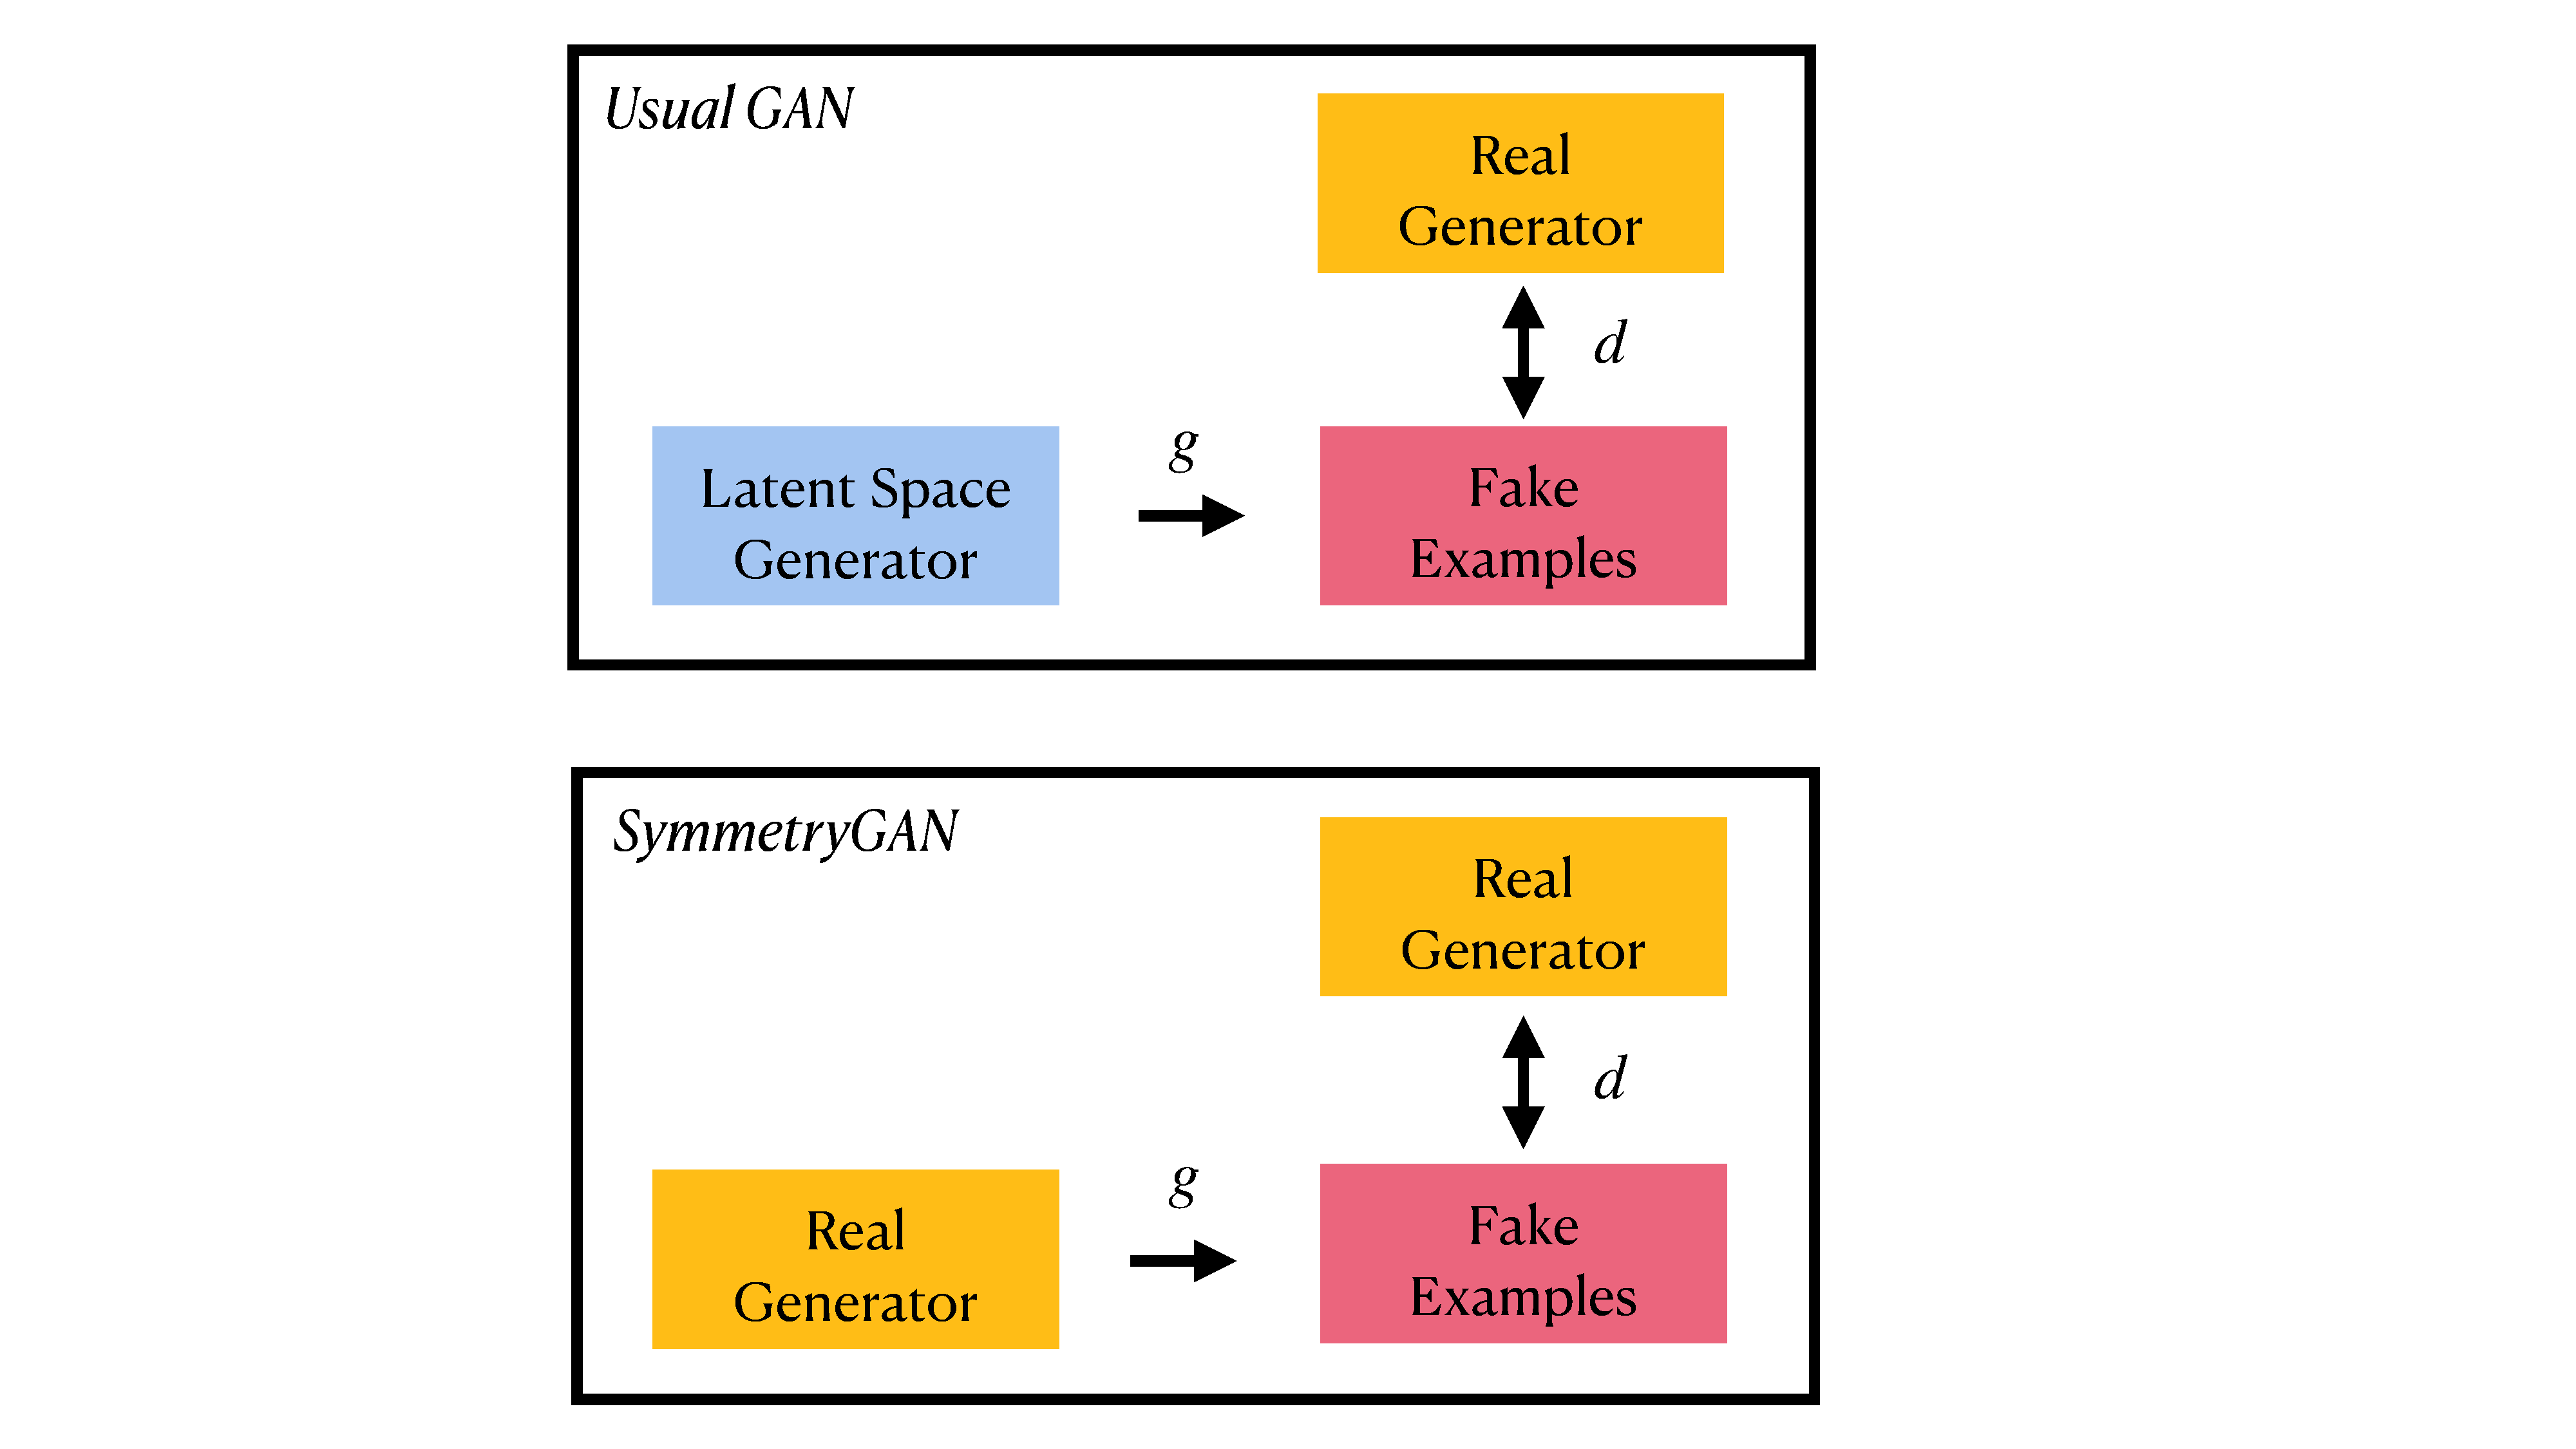
\includegraphics[width=0.6\textwidth]{figures/chapter-09/SchematicSymmetry2.pdf}
    \caption[Architectural comparison of standard GAN and SymmetryGAN for automated symmetry discovery.]{Schematic comparison of training architectures for (top) a standard Generative Adversarial Network (GAN) and (bottom) the proposed SymmetryGAN framework for automated symmetry discovery in particle physics data.
    %
    In a standard GAN, the generator $g: \mathcal{Z} \to \mathcal{X}$ maps random noise $z \sim p_z$ to synthetic data samples, while the discriminator $d: \mathcal{X} \to [0,1]$ attempts to distinguish real data $x \sim p_{\text{data}}$ from generated samples $g(z)$. The adversarial training objective drives $g$ to match the data distribution without explicit physics constraints.
    %
    The SymmetryGAN architecture modifies this framework with a symmetry transformation module $g_\theta: \mathcal{X} \to \mathcal{X}$, parametrized by learnable parameters $\theta$, which acts on both real samples. The discriminator receives transformed pairs $(x, T_\theta(x)),$ learning to identify distribution preserving transformations. When the discriminator cannot distinguish between a sample and its transformed version, the transformation $T_\theta$ represents an symmetry of the distribution.
    %
    The inertial reference dataset, while not explicitly shown in this diagram, is incorporated directly into the generator architecture in \cref{sec:empirical-experiments}}
    \label{fig:symmetrygan-schematic}
\end{figure}
    \cref{fig:symmetrygan-schematic} shows the modified GAN architecture of \textsc{SymmetryGAN}.
    
    \subsection{Machine Learning with Inertial Restrictions}
    The incorporation of inertial reference densities, as established in \cref{subsec:inertial_densities}, presents both theoretical necessity and practical challenges.
    %
    These restrictions can be implemented through three distinct approaches.
    \begin{enumerate}
        \item \textbf{Simultaneous discrimination}:
            %
            In this approach, discriminators evaluate transformations on both the target dataset and samples from the inertial density.
            %
            The loss function is extended to include terms from the inertial distribution \(p_I\)
            \[
                \widetilde L[g,d,d_I] = L[g,d] + \lambda L_I[g,d_I]
            \]
            where \(d_I\) is a separate discriminator network specialized for the inertial distribution.
            %
            This method offers maximal flexibility, allowing discovery of symmetries even when the inertial distribution's symmetries are not known analytically.
            %
            However, it requires the ability to sample from \(p_I\) which becomes problematic for improper priors like uniform distributions on \(\mathbb{R}^n\).
        \item \textbf{Two stage selection}:
            %
            This approach involves first identifying all PDF preserving maps, then filtering for those preserving the inertial density.
            %
            The two stage approach decouples the symmetry discovery problem into training multiple generators to find PDF preserving transformations of the target data and \textit{post hoc} verifying which transformations also preserve \(p_I\)
            %
            While conceptually clean, this method proves computationally wasteful, as the space of PDF preserving maps vastly exceeds the space of true symmetries.
        \item \textbf{Upfront restriction}:
            %
            Here one constrains the generator architecture to only produce transformations that preserve the inertial density by construction in the first place, using prior knowledge about \(p_I\).
    \end{enumerate}
    
    It is this third approach that is adopted in the \textsc{SymmetryGAN} implementation.
    %
    When the inertial distribution is uniform on \(\mathbb{R}^n\) the generator should be restricted to equiareal maps---transformations with unit Jacobian determinant, as shown in \cref{eq:equiareal-maps}.
    %
    The intersection of the equiareal group and affine group \(\operatorname{Aff}_n(\R)\) corresponds to the affine special linear group \(\mathbb{A}SL^\pm_n(\mathbb{R})\) and its extensions.

    The upfront restriction method offers computational efficiency gains by searching only among valid symmetries in addition to theoretical guarantees that discovered transformations are true symmetries.
    %
    It also simplifies training without multiple discriminators or \textit{post hoc} verification.

    The restriction to affine equiareal maps, while limiting, captures a rich class of symmetries including rotations, reflections, shears, and all their compositions.
    %
\begin{theorem}[Iwasawa Decomposition of the Affine Group~\cite{iwasawa_types_1949}]
\label{thm:iwasawa_affine}
Let 
\[
    \operatorname{Aff}_n(\R)= GL_n(\R)\ltimes\R^n
\]
be the real affine group.  Define the subgroups
\[
\begin{aligned}
Z &= \{\pm I_n\}\cong \mathbb{Z}_2,\\
K &= SO(n),\\
A &= \bigl\{D(\vb r)=\operatorname{diag}(r_1,\dots,r_n)\;\big|\;r_i\in(0,\infty)\bigr\},\\
N &= \bigl\{S(u) \;\big|\;S_{ii}=1,\ S_{i < j}\in\R, S_{i>j}=0\bigr\},\\
V &= \qty{\vb v \mid v_i\in\R }\cong\R^n.
\end{aligned}
\]
Then every element $M\in\operatorname{Aff}_n(\R)$ admits a unique factorisation
\[
M \;=\;
\sqrt{|\det M|}\;\bigl(\pm I_n\bigr)^{\frac{1-\text{sgn}(\det M)}{2}}
\;R(\vb\theta)\;D(\vb r)\;S(u) + \vb v,
\]
where
\(
\pm I_n\in Z,\quad R(\vb\theta)\in K,\quad D(\vb r)\in A,\quad S(u)\in N,\quad \vb v\in V.
\)
\end{theorem}
In two dimensions these matrices take the form
\begin{gather}
I_2=\begin{bmatrix}1&0\\0&-1\end{bmatrix},\\
R(\theta)=\begin{bmatrix}\cos\theta & -\sin\theta\\
\sin\theta & \cos\theta\end{bmatrix},\\
D(r)=\begin{bmatrix}r & 0\\0 & r^{-1}\end{bmatrix},\\
S(u)=\begin{bmatrix}1 & u\\0 & 1\end{bmatrix},\\
v=\begin{bmatrix}v_1\\v_2\end{bmatrix}.
\end{gather}
Hence every $g\in\operatorname{Aff}_2(\R)$ admits the six parameter representation
\[
g(x)=\sqrt{|d|}\,\bigl(I_2\bigr)^{\frac{1-\text{sgn}(d)}{2}}
R(\theta)\,D(r)\,S(u)\,x \;+\;v,
\qquad d=\det g,
\]
which is well suited to gradient based optimization over the space of affine symmetries.

\subsection{Deep learning implementation details.}

    The practical implementation of \textsc{SymmetryGAN} requires careful attention to architectural choices, training dynamics, and numerical stability.
    %
    The framework's success depends on balancing the adversarial training process while maintaining the theoretical properties that enable symmetry discovery.
    
    For linear symmetries, the generator directly parametrises transformation matrices.
    %
    Rather than using fully connected layers, the generator outputs parameters of the Iwasawa decomposition, ensuring all generated transformations lie within the constrained search space.
    %
    This architectural choice provides interpretability, where each parameter has clear geometric meaning, stability, by avoiding ill conditioned matrices through structured parametrisation, and efficiency, by reducing the parameter count compared to unconstrained matrices from \(n^2\) to \(\nicefrac{n(n-1)}{2}.\)

    To investigate specific symmetry subgroups, the loss function can further incorporate additional constraints.
    %
    For example, to find cyclic symmetries \(\mathbb{Z}_q\) the loss can be augmented to encourage \(g^q = \mathbbm{1}\).
    \[
        \label{eq:cyclic-loss}
        L_{\text{cyclic}}[g,d] = L_{\text{BCE}}[g,d] + \alpha \sum_{i} ||g^q(x_i) - x_i||^2.
    \]

    The discriminator architecture should follow standard practices for the data domain.
    %
    For low dimensional examples, simple feedforward networks with \(2-3\) hidden layers suffice.

    Analysing the loss landscape reveals its topological structure.
    %
    For simple distributions like Gaussians, the loss landscape contains distinct maxima corresponding to each symmetry, separated by deep valleys.
    %
    This topology explains why random initialisation reliably discovers different symmetries.
    %
    The generator converges to the nearest local maximum, which corresponds to a true symmetry, and there is no reason to expect that the nearest local maximum for any given random initialisation should be the identity map.

    The framework demonstrates remarkable robustness to hyperparameter choices.
    %
    Across experiments with Gaussian mixtures and particle physics data, a range of hyperparameter settings achieve consistent symmetry discovery.

    \subsection{Verification.}
    A few different checks can be applied to verify that the discovered transformation represents a true symmetry.
    \begin{itemize}
        \item \textbf{Visual inspection}: Visually inspecting low dimensional slices of the original and transformed data serves as a simple sniff test.
        \item \textbf{Loss value}: True symmetries always achieve a loss of \(2\log2\) at convergence. Hence measuring the loss function at discovered transformations can validate whether the transformation is a symmetry or not.
        \item \textbf{Distribution matching}: Statistical divergences between \(X\) and \(g(X)\) such as the KL divergence measure whether the two datasets have the same probability density or not.
        \item Invariant verification: known invariants, such as moments, should be identical between the distributions.
    \end{itemize}
    
    \subsection{Other symmetry discovery methods.}
        The landscape of symmetry discovery in machine learning has evolved considerably, with approaches ranging from classical statistical methods to modern deep learning architectures.
        %
        Understanding \textsc{SymmetryGAN}'s position within this ecosystem illuminates both its unique contributions and its connections to broader methodological trends.

        Classical statistical approaches traditionally rely on hypothesis testing and moment matching.
        %
        These methods typically test specific, predefined symmetry hypotheses by relying on low dimensional projections or summary statistics.
        %
        They struggle with high dimensional data or complex symmetry groups and require extensive domain knowledge to formulate appropriate tests.

        The Cramer-von Mises~\cite{von_mises_wahrscheinlichkeit_1928, cramer_composition_1928} and Anderson-Darling tests~\cite{anderson_asymptotic_1952} exemplify this approach to check whether transformed data follows the same distribution as the original.
        %
        While rigorous, these methods scale poorly and cannot discover unexpected symmetries, they can only validate known symmetries.

        Machine learning methods introduced automation to the symmetry discovery process.
        %
        Methods like Group-Invariant Autoencoders~\cite{Hao2023LorentzAutoencoders} learn representations invariant to known symmetry groups but cannot discover unknown symmetries
        %
        Spatial Transformer Networks~\cite{Jaderberg2015SpatialNetworks} learn task-specific transformations but don't explicitly identify symmetries \textit{per se}.
        %
        Maximum Mean Discrepancy approaches~\cite{tolstikhin_minimax_2016} and other kernel methods can test symmetry but struggle with continuous groups.

        Contemporary deep learning methods have introduced a range of innovations to the field.
        %
        Lie Group Learning Networks directly parametrise Lie algebra generators~\cite{gabel_learning_2023}.
        %
        Such methods have excellent theoretical grounding, and physically interpretable parameters.
        %
        They are, however, restricted to continuous symmetries, and require complex optimisation for convergence.
        %
        Latent LieGAN (LaLiGAN) enables the discovery nonlinear symmetries via latent space linearization~\cite{yang_latent_2024}.
        %
        It made strides in handling non-linear group actions, but the additional complexity leads to potential latent space artifacts

        \textsc{SymmetryGAN} exemplifies several important trends in modern machine learning for HEP.
        %
        Methods have broadly benefited from incorporating domain knowledge through architectural constraints and loss terms.
        %
        In general the rise of equivariant learning has driven the move beyond invariance to discover the underlying symmetry structure.
        
        \textsc{SymmetryGAN} also exemplies the trend towards interpretability by producing human understandable symmetry parameters rather than opaque features.
        %
        The method is however limited in its restriction to parametrisable symmetry classes.
        %
        It also exclusively enables symmetry discovery, the task of identifying elements of the symmetry group of a dataset.
        %
        Although the work does provide some steps towards symmetry inference, the task of identifying and classifying the symmetry group as a whole, it remains challenging to infer complete symmetry group structure from discovered elements.
        
        The field continues to evolve rapidly, with \textsc{SymmetryGAN} representing a significant step toward automated, theoretically grounded symmetry discovery.
        %
        Its success in particle physics applications, detailed in the following section, demonstrates the practical value of this principled approach to uncovering hidden invariances in complex data.

\section{Empirical experiments.}
\label{sec:empirical-experiments}
        The theoretical machinery of \textsc{SymmetryGAN}, with its rigorous statistical framework and inertial reference densities, proves its worth through empirical validation.
        %
        Moving from abstract formulations to concrete applications reveals both the method's effectiveness and challenges that might drive future research.
        %
        This section details the application of this method on carefully controlled Gaussian experiments to complex collider data, demonstrating how \textsc{SymmetryGAN} bridges the gap between mathematical elegance and practical discovery.

        \subsection{Gaussian experiments.}
            The choice to begin with Gaussian distributions reflects more than mere mathematical convenience; it represents a strategic approach to validating a novel methodology.
            %
            Gaussians offer analytically tractable loss landscapes that allow direct comparison between theoretical predictions and empirical results, serving as a crucial proof of concept before tackling high dimensional HEP data.

            \subsubsection{One-dimensional Gaussian.}
                The simplest non-trivial test case consists of a Gaussian distribution \(\mathcal{N}(0.5,1.0)\) with a reflection symmetry about \(x=0.5\).
                %
                This apparently simple example harbours surprising richness.
                %
                The disconnected nature of the symmetry space in even this simple example demonstrates the training dynamics in a \textsc{SymmetryGAN.}

                The distribution admits precisely two linear symmetries: the identity transformation \(g(x)=x\) and the reflection \(g(x)=1-x\).
                %
                When the generator is parametrised as an arbitrary one dimensional affine transformation, \(g(x)=b+cx\), the analytic loss landscape has the topology shown in \cref{fig:Z2analytic}.
                %
                The two maxima corresponding to these symmetries are separated by a deep valley at \(c=0\), creating a disconnected solution space.
 \begin{figure}
     \centering
     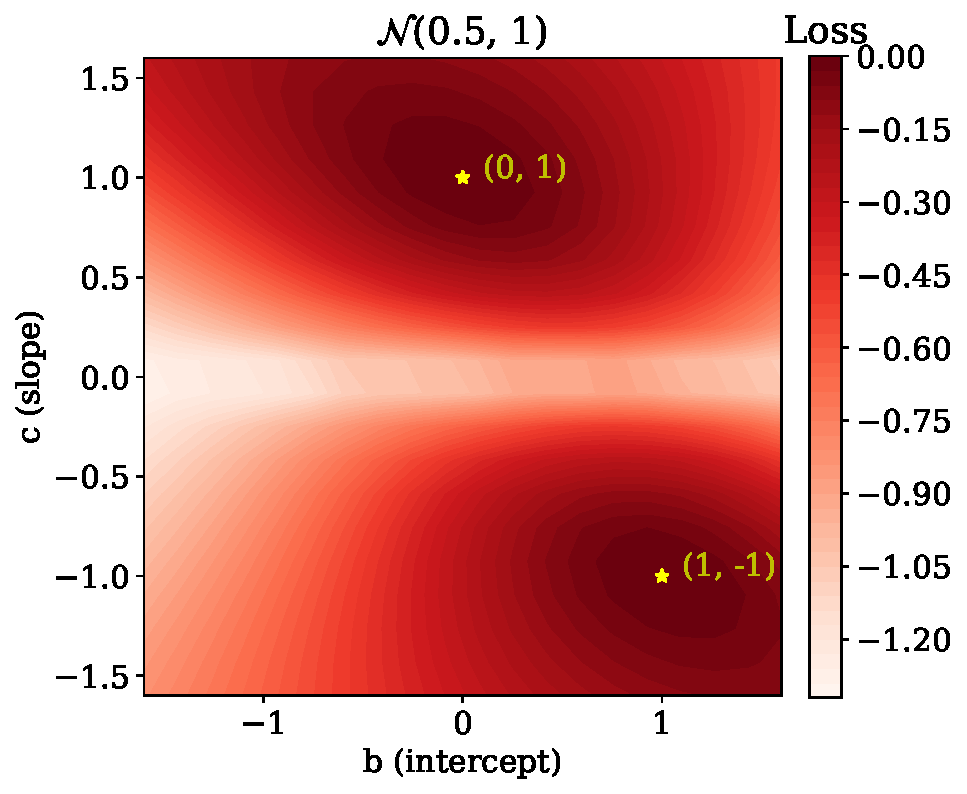
\includegraphics[width=0.6\linewidth]{figures/chapter-09/Z2analytic.pdf}
     \caption{Analytic loss landscape for the one-dimensional uniform distribution $\mathcal{N}((0.5,1))$ under affine transformations $g(x) = b + cx$. The landscape exhibits two distinct maxima (indicated by stars) corresponding to the identity transformation $(b,c) = (0,1)$ and reflection $(b,c) = (1,-1)$, separated by a deep valley at $c = 0$.
     %
     This topological barrier creates a disconnected solution space that deterministically routes optimisation trajectories based on initial parameter values.
     }
     \label{fig:Z2analytic}
 \end{figure}               
                The empirical results validate the theoretical predictions with remarkable precision.
                %
                Random initialisation of parameters \((b_i, c_i) \sim \mathcal{U}([-5, 5]^2)\) leads to convergence at one of two distinct clusters: \((b_f, c_f) = (0, 1)\) for the identity or \((1, -1)\) for the reflection as can be seen in \cref{fig:Z2numeric}.
                %
                The loss barrier at \(c=0\) acts as a watershed, deterministically routing the optimisation based on the sign of the initial slope.
                %
                This behaviour illuminates that the loss landscape topology directly determines the discoverable symmetry structure.
\begin{figure}
    \centering
    \begin{subfigure}[b]{0.31\textwidth}
        \centering
        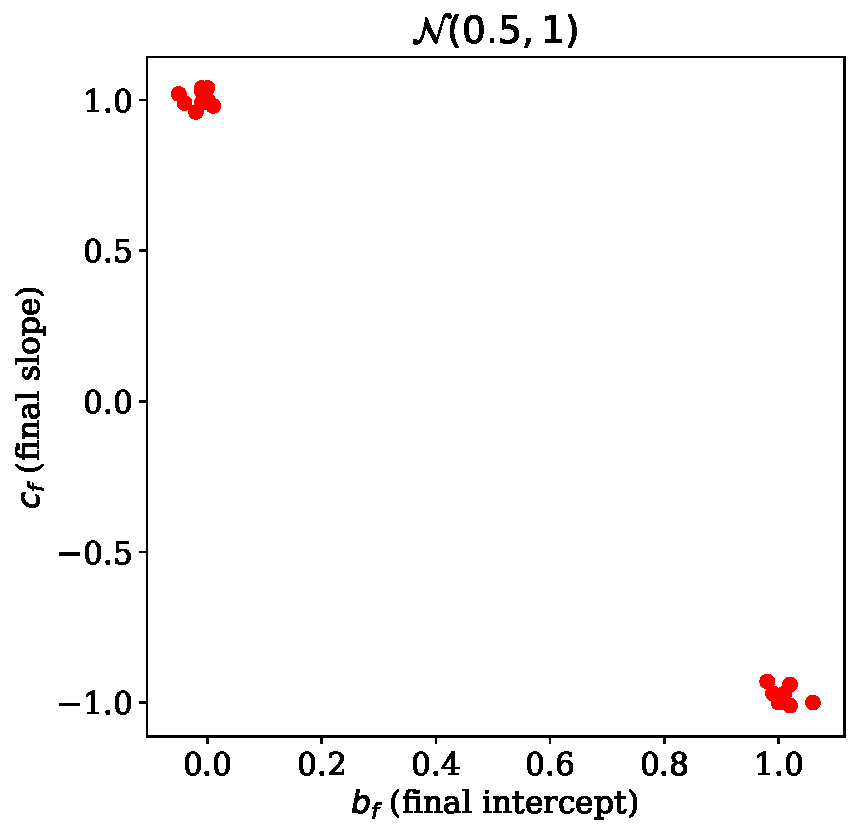
\includegraphics[width=\textwidth]{figures/chapter-09/b_fc_f.pdf}
        \caption{}
        \label{fig:Z2numeric_i}
    \end{subfigure}
    \hfill
    \begin{subfigure}[b]{0.31\textwidth}
        \centering
        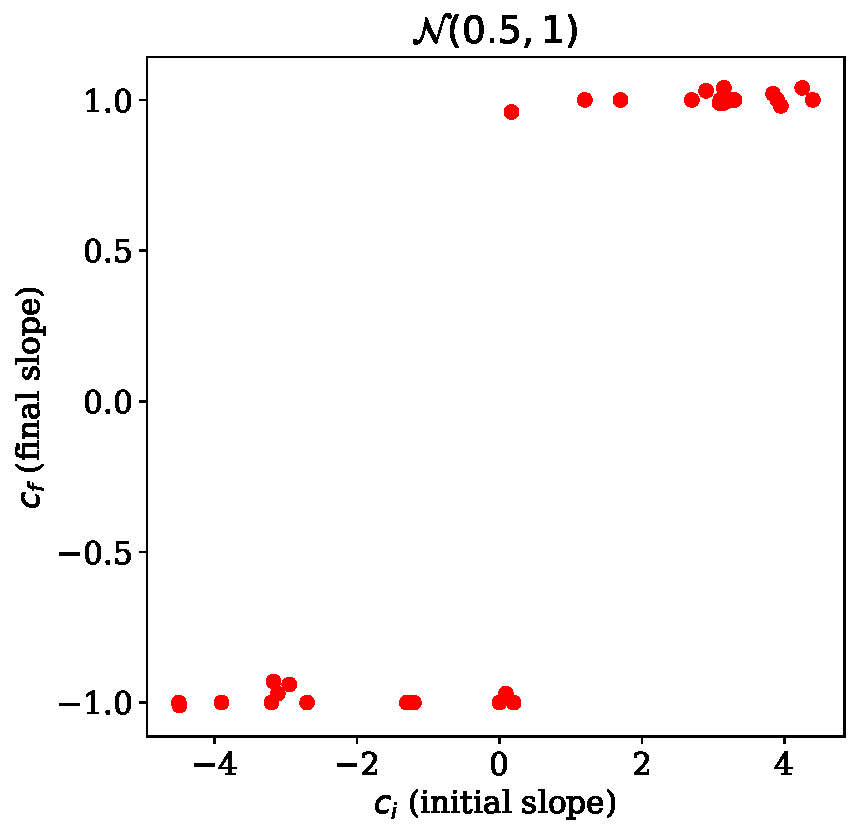
\includegraphics[width=\textwidth]{figures/chapter-09/c_ic_f.pdf}
        \caption{}
        \label{fig:Z2numeric_ii}
    \end{subfigure}
    \hfill
    \begin{subfigure}[b]{0.31\textwidth}
        \centering
        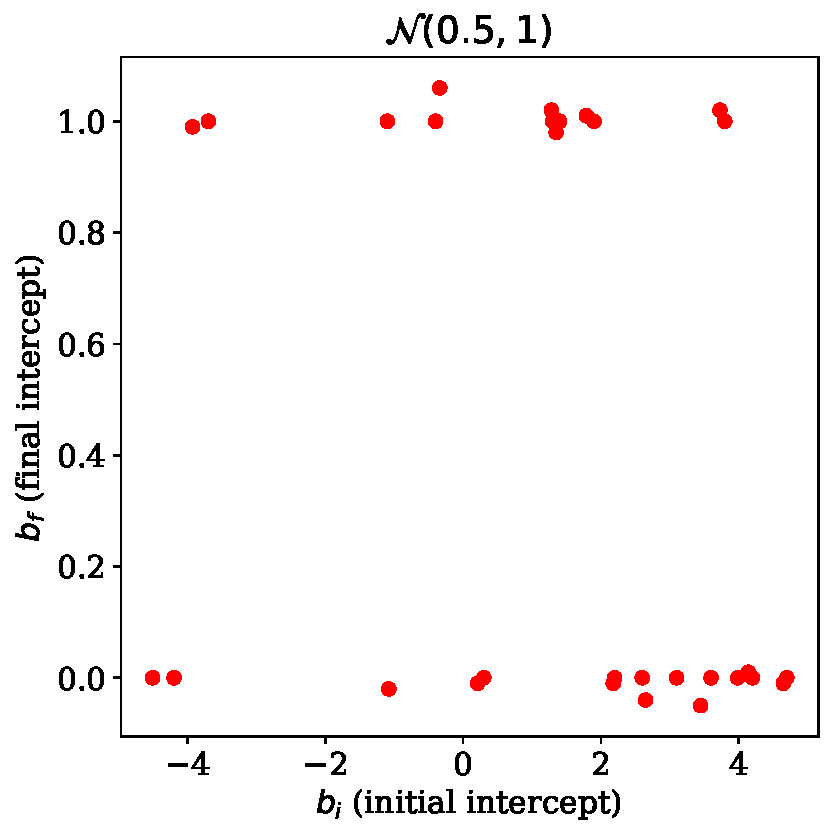
\includegraphics[width=\textwidth]{figures/chapter-09/b_ib_f.pdf}
        \caption{}
        \label{fig:Z2numeric_iii}
    \end{subfigure}
    \caption[Empirical validation of \textsc{SymmetryGAN} on 1 dimensional Gaussian data showing convergence to discrete symmetries based on initial conditions.]{Empirical validation of \textsc{SymmetryGAN} on 1 dimensional Gaussian data showing convergence to discrete symmetries based on initial conditions.
    %
    Random initialisation with $(b_i, c_i) \sim \mathcal{U}([-5, 5]^2)$ leads to convergence at two distinct fixed points. (a) Distribution of final parameters $(b_f, c_f)$ reveals two clusters at $(0,1)$ and $(1,-1)$, corresponding to the identity and reflection symmetries respectively. (b) Deterministic routing based on initial slope: $c_i > 0$ converges to identity $(c_f = 1)$ while $c_i < 0$ converges to reflection $(c_f = -1)$, with a sharp phase transition at $c_i = 0$. (c) Final intercept $b_f$ shows no correlation with initial value $b_i$, demonstrating that the loss landscape has no barrier in intercept space.}
    \label{fig:Z2numeric}
\end{figure}
            \subsubsection{Two dimensional Gaussians.}
                Two dimensional Gaussian examples increase the complexity while maintaining analytical tractability.
                %
                Consider first the standard bivariate normal \(N_{1, 1} = \mathcal{N}(\mathbf{0}, \mathbbm{1}_2)\), which possesses the full orthogonal group \(O(2)\) as its symmetry group.
                %
                When the generator is restricted to the form
{\setlength{\arraycolsep}{12pt}
\[
  \label{eq:SO2_generator}
  g(x)=\begin{bmatrix}
     c & s\\
    -s & c
  \end{bmatrix}x
\]
}
                \textsc{SymmetryGAN} would be expected to discover that only transformations satisfying \(c^2 + s^2 = 1\) represent true symmetries.
                %
                As can be seen in \cref{fig:SO2-i}, the empirical results demonstrate the method's ability to learn this constraint without explicit enforcement.
                %
                Starting from random initialisations within \([-1, 1]^2\), the learned parameters consistently converge to the unit circle, validating that \textsc{SymmetryGAN} can discover not just discrete symmetries but continuous symmetry manifolds.
                %
                This represents a significant achievement: the neural network learns the algebraic constraint defining \(SO(2)\) purely from data.
\begin{figure}
    \centering
    \begin{subfigure}[b]{0.45\textwidth}
        \centering
        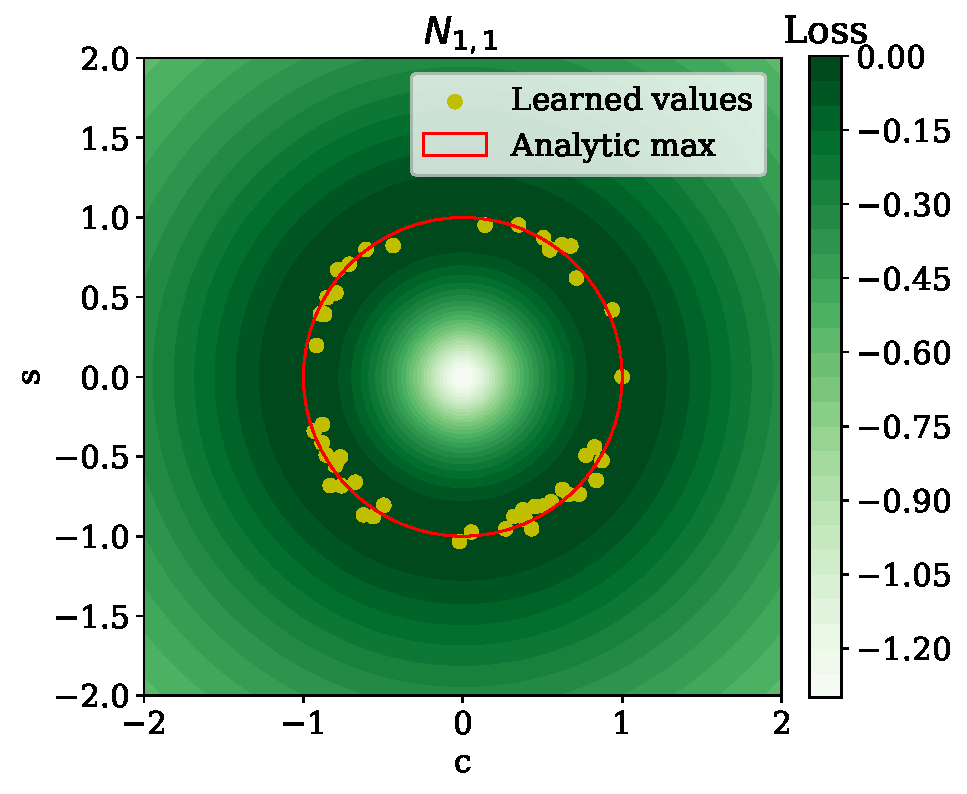
\includegraphics[width=\textwidth]{figures/chapter-09/SO2symmAnalytic.pdf}
        \caption{}
        \label{fig:SO2-i}
    \end{subfigure}
    \hfill
    \begin{subfigure}[b]{0.45\textwidth}
        \centering
        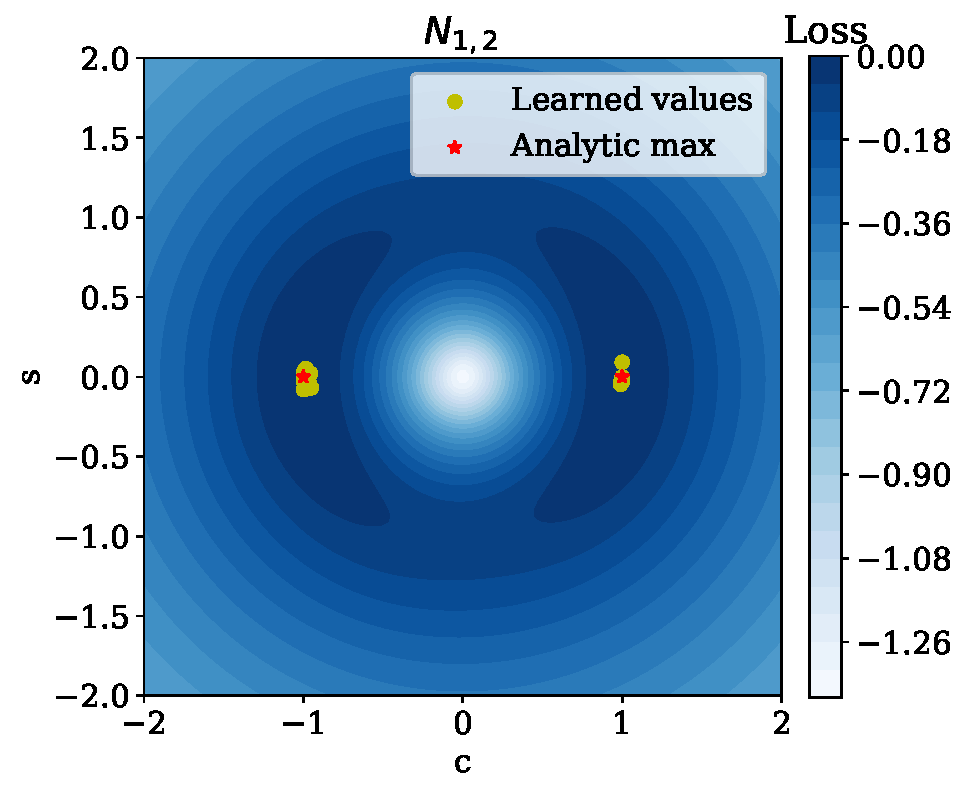
\includegraphics[width=\textwidth]{figures/chapter-09/4O2asymmAnalytic.pdf}
        \caption{}
        \label{fig:SO2-iii}
    \end{subfigure}
    \caption[Loss landscapes demonstrating \textsc{SymmetryGAN's} ability to discover continuous $SO(2)$ and discrete $V_4$ symmetries in isotropic and anisotropic 2D Gaussians.]{Analytic loss landscapes for two dimensional Gaussian distributions under rotation like transformations $g(\mathbf{x}) = \begin{pmatrix} c & -s \\ s & c \end{pmatrix}\mathbf{x}$, with empirically discovered symmetries overlaid as scatter points. (a) Isotropic Gaussian $\mathcal{N}(\mathbf{0}, \mathbbm{1})$ exhibits continuous $SO(2)$ symmetry, with loss maxima forming a circle at $c^2 + s^2 = 1$. The discovered symmetries densely populate this manifold, confirming the theoretical prediction. (b) Anisotropic Gaussian $\mathcal{N}(\mathbf{0}, \text{diag}(1,2))$ possesses only discrete Klein four--group symmetries $V_4$, with isolated maxima at $(c,s) \in \{(\pm 1, 0), (0, \pm 1)\}$. The symmetry breaking from continuous to discrete group structure is induced by the non-uniform covariance. Darker regions indicate higher loss values; stars mark theoretical optima.}
    \label{fig:SO2}
\end{figure}
\begin{figure}
    \centering
    \begin{subfigure}[b]{0.31\textwidth}
        \centering
        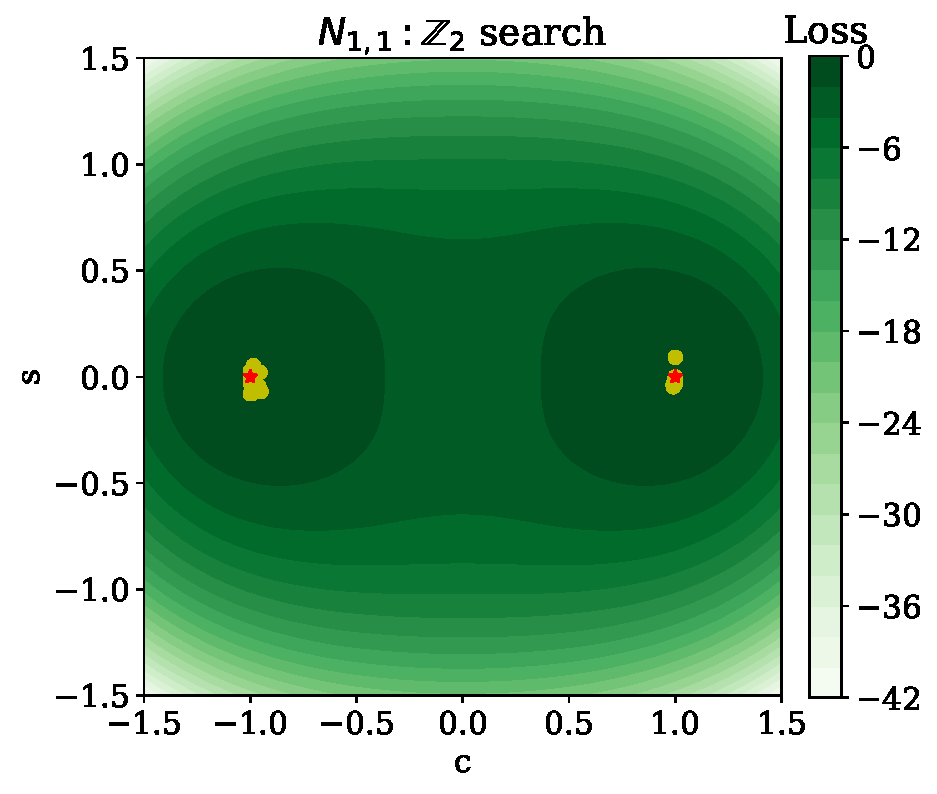
\includegraphics[width=\textwidth]{figures/chapter-09/C2MSE.pdf}
        \caption{}
        \label{fig:MSE_i}
    \end{subfigure}
    \hfill
    \begin{subfigure}[b]{0.31\textwidth}
        \centering
        \includegraphics[width=\textwidth]{figures/chapter-09/C3MSE.pdf}
        \caption{}
        \label{fig:MSE_ii}
    \end{subfigure}
    \hfill
    \begin{subfigure}[b]{0.31\textwidth}
        \centering
        \includegraphics[width=\textwidth]{figures/chapter-09/C7MSE.pdf}
        \caption{}
        \label{fig:MSE_iii}
    \end{subfigure}
    \caption[Controlled discretization of continuous $SO(2)$ symmetry into cyclic subgroups $\mathbb{Z}_q$ via constraint enforcement.]{Controlled symmetry breaking in the isotropic Gaussian $\mathcal{N}(\mathbf{0}, \mathbbm{1})$ through cyclic constraint enforcement. The loss function is augmented with a mean squared error term $\alpha \|g^q(\mathbf{x}) - \mathbf{x}\|^2$ that enforces $q-$fold cyclic symmetry. The continuous $SO(2)$ symmetry observed in \cref{fig:SO2-i} is discretised into cyclic subgroups: (a) $\mathbb{Z}_2$ symmetry with $q=2$, showing two antipodal maxima at $(c,s) = (\pm 1, 0)$; (b) $\mathbb{Z}_3$ symmetry with $q=3$, displaying three maxima at the cube roots of unity; (c) $\mathbb{Z}_7$ symmetry with $q=7$, exhibiting seven equally spaced maxima on the unit circle. The discovered symmetries (scatter points) precisely align with the $q^{\text{th}}$ roots of unity, validating the theoretical prediction that the cyclic constraint induces symmetry discovery of discrete components. Darker regions indicate higher loss values, stars indicate analytic maxima.}
    \label{fig:MSE}
\end{figure}               

                The two dimensional Gaussian example also allows us to test the approach described in \cref{eq:cyclic-loss}.
                %
                \cref{fig:MSE} shows the discovered symmetries for the \(N_{1, 1}\) distribution when the loss function is augmented with the constraint \cref{eq:cyclic-loss}, for \(q = 2, 3,\) and \(7\), with \(\alpha = 0.1\).
                %
                Both the analytic loss landscape and \textsc{SymmetryGAN}'s output confirm that the continuous \(SO(2)\) symmetry is split into discrete symmetries at the \(q^{th}\) roots of unity upon the inclusion of the mean squared error term.

                One could also consider a two dimensional Gaussian with a non-trivial covariance matrix, such as \(N_{1, 2} = \mathcal{N}(\mathbf{0}, \text{diag}(1, 2)\).
                %
                The full symmetry group of this distribution is highly non-trivial and is described below, but among other features, it contains as a subgroup the Klein \(4-\)group \(V_4 = \qty{\mathbbm{1}, -\mathbbm{1}, \sigma_3, -\sigma_3}\) for the Pauli matrix \(\sigma_3\).
                %
                When \textsc{SymmetryGAN} is limited to transformations of the form \cref{eq:SO2_generator}, it discovers the Klein \(4-\)group \(V_4\) as demonstrated in \cref{fig:SO2-iii}.
                %
                When the generator is allowed to search for general linear transformations inside \(\operatorname{Aff}_2(\mathbb{R})\), it discovers the full symmetry group that comprises the aforementioned Klein \(4-\)group as well as transformations involving dilatations.

                \cref{fig:AGL2symm} shows the discovered symmetries for the \(N_{1, 1}\) distribution and \cref{fig:AGL2asymm} shows the discovered symmetries for \(N_{1, 2}\) when the generator is able to discover general affine transformations in \(\operatorname{Aff}_2(\R).\)
\begin{figure}
    \centering
    \begin{subfigure}[b]{0.31\textwidth}
        \centering
        \includegraphics[width=\textwidth]{figures/chapter-09/6O2d-tsymm.pdf}
        \caption{}
        \label{fig:AGL2symm_i}
    \end{subfigure}
    \hfill
    \begin{subfigure}[b]{0.31\textwidth}
        \centering
        \includegraphics[width=\textwidth]{figures/chapter-09/6GL2symmRU.pdf}
        \caption{}
        \label{fig:AGL2symm_ii}
    \end{subfigure}
    \hfill
    \begin{subfigure}[b]{0.31\textwidth}
        \centering
        \includegraphics[width=\textwidth]{figures/chapter-09/6GL2symmAB.pdf}
        \caption{}
        \label{fig:AGL2symm_iii}
    \end{subfigure}
    \caption[Orthogonal slices of $\operatorname{Aff}_2(\mathbb{R})$ symmetries for isotropic Gaussian.]{Symmetry discovery in the full affine group $\operatorname{Aff}_2(\mathbb{R})$ for the isotropic Gaussian $\mathcal{N}(\mathbf{0}, \mathbbm{1})$, decomposed via Iwasawa parametrization $g = \sqrt{|d|} I^{\frac{1-\text{sgn}(d)}{2}} \cdot R(\theta) \cdot D(r) \cdot S(u) + \mathbf{v}$. Three orthogonal slices through the 6 dimensional loss landscape reveal the symmetry structure: (a) Determinant-rotation space $(d, \theta)$ shows continuous maxima along $d = \pm 1$ (vertical red lines) for all rotation angles. (b) Dilation-shear space $(r, u)$ exhibits a unique maximum at $(r, u) = (1, 0)$ (red star), indicating that only uniform scaling preserves the isotropic structure. (c) Translation space $(v_1, v_2)$ peaks at the origin (red star), verifying that the centred Gaussian admits no translational symmetries. Empirically discovered transformations (yellow points) cluster precisely at the theoretical optima, validating the analytic predictions.}
    \label{fig:AGL2symm}
\end{figure}
\begin{figure}
    \centering
    \begin{subfigure}[b]{0.31\textwidth}
        \centering
        \includegraphics[width=\textwidth]{figures/chapter-09/6GL2asymmDU.pdf}
        \caption{}
        \label{fig:AGL2asymm_i}
    \end{subfigure}
    \hfill
    \begin{subfigure}[b]{0.31\textwidth}
        \centering
        \includegraphics[width=\textwidth]{figures/chapter-09/6GL2asymmTR.pdf}
        \caption{}
        \label{fig:AGL2asymm_ii}
    \end{subfigure}
    \hfill
    \begin{subfigure}[b]{0.31\textwidth}
        \centering
        \includegraphics[width=\textwidth]{figures/chapter-09/6GL2asymmAB.pdf}
        \caption{}
        \label{fig:AGL2asymm_iii}
    \end{subfigure}
    \caption[Discrete symmetry structure of anisotropic Gaussian in $\text{Aff}_2(\mathbb{R})$ discovered by \textsc{SymmetryGAN}.]{Symmetry discovery in $\text{Aff}_2(\mathbb{R})$ for the anisotropic Gaussian $\mathcal{N}(\mathbf{0}, \text{diag}(1,2))$, revealing discrete symmetry breaking compared to the isotropic case (\cref{fig:AGL2symm}). The anisotropic covariance structure constrains the symmetry group to a supergroup of the Klein four-group $V_4$: (a) Determinant-shear space $(d, u)$ exhibits two isolated maxima (red stars) at $(d, u) \in \{(1, 0), (-1, 0)\}$, corresponding to orientation-preserving and orientation-reversing transformations with no shear. (b) Dilation-rotation space $(r, \theta)$ shows four discrete maxima (red stars) at $(r, \theta) \in \{(1, 0), (1, \pi), (\sqrt{2}, \pi/2), (\sqrt{2}, 3\pi/2)\}$, representing identity, $\pi$-rotation, and the two coordinate flips scaled by $\sqrt{2}$ to account for the eigenvalue ratio. (c) Translation space $(v_1, v_2)$ remains peaked at the origin (red star), confirming no translational symmetries. The discovered transformations (yellow points) cluster at these discrete locations, demonstrating how anisotropy breaks continuous symmetries into a discrete group.}
    \label{fig:AGL2asymm}
\end{figure}
            \subsubsection{Gaussian Mixture Models}
                The power of \textsc{SymmetryGAN} becomes more apparent when applied to Gaussian mixture models with complex symmetry groups.
                %
                Three such examples are considered, inspired by the the examples in~\cite{fisher_boltzmann_2018}.
                %
                The first is a one dimensional bimodal distribution,
                \[
                    p(x) = \frac{1}{2} \mathcal{N}(-1, 1) + \frac{1}{2} \mathcal{N}(1, 1)
                \]
                which possesses the cyclic group \(\mathbb{Z}_2 = \qty{x \mapsto \pm x}\) as its symmetry group.
                %
                The discovered symmetries are shown in \cref{fig:otherdistributions-1D}.
\begin{figure}
    \centering
    \begin{subfigure}[b]{0.4\textwidth}
        \centering
        \includegraphics[height=\textwidth]{figures/chapter-09/1d_bimodalplot.pdf}
        \caption{}
        \label{fig:otherdistributions_1Di}
    \end{subfigure}
    \begin{subfigure}[b]{0.4\textwidth}
        \centering
        \includegraphics[height=\textwidth]{figures/chapter-09/1d_bimodalsymm.pdf}
        \caption{}
        \label{fig:otherdistributions_1Dii}
    \end{subfigure}
    \caption[\textsc{SymmetryGAN}'s predictions for a bimodal Gaussian mixture with $\mathbb{Z}_2$ reflection symmetry and corresponding loss landscape validation.]{Symmetry discovery for a one dimensional bimodal Gaussian mixture $p(x) = \frac{1}{2}\mathcal{N}(-1, 1) + \frac{1}{2}\mathcal{N}(1, 1)$ possessing $\mathbb{Z}_2$ symmetry. (a) Probability density function showing two symmetric modes at $x = \pm 1$ with equal weights and variances, creating a distribution invariant under reflection about the origin. (b) Analytic loss landscape in the $(b, c)$ parameter space for linear transformations $g(x) = b + cx$, with empirically discovered symmetries overlaid (blue points). The landscape exhibits two distinct maxima at $(b, c) = (0, 1)$ and $(0, -1)$, corresponding to the identity and reflection transformations respectively. The discovered symmetries cluster precisely at these theoretical optima, confirming that \textsc{SymmetryGAN} correctly identifies the cyclic group $\mathbb{Z}_2 = \{x \mapsto \pm x\}$ as the complete symmetry group of the distribution.}
    \label{fig:otherdistributions-1D}
\end{figure}
\begin{figure}
    \centering
    \begin{subfigure}[b]{0.27\textwidth}
        \centering
        \includegraphics[height=\textwidth]{figures/chapter-09/2d_circularplot.pdf}
        \caption{}
        \label{fig:otherdistributions_2D_i}
    \end{subfigure}
    \hfill
    \begin{subfigure}[b]{0.28\textwidth}
        \centering
        \includegraphics[height=\textwidth]{figures/chapter-09/2doctagonalrotations.pdf}
        \caption{}
        \label{fig:otherdistributions_2D_ii}
    \end{subfigure}
    \hfill
    \begin{subfigure}[b]{0.27\textwidth}
        \centering
        \includegraphics[height=\textwidth]{figures/chapter-09/2doctagonalreflections.pdf}
        \caption{}
        \label{fig:otherdistributions_2D_iii}
    \end{subfigure}
    
    \vspace{0.3cm}
    
    \begin{subfigure}[b]{0.27\textwidth}
        \centering
        \includegraphics[height=\textwidth]{figures/chapter-09/2d_squareplot.pdf}
        \caption{}
        \label{fig:otherdistributions_2D_iv}
    \end{subfigure}
    \hfill
    \begin{subfigure}[b]{0.28\textwidth}
        \centering
        \includegraphics[height=\textwidth]{figures/chapter-09/2dsquarerotations.pdf}
        \caption{}
        \label{fig:otherdistributions_2D_v}
    \end{subfigure}
    \hfill
    \begin{subfigure}[b]{0.27\textwidth}
        \centering
        \includegraphics[height=\textwidth]{figures/chapter-09/2dsquarereflections.pdf}
        \caption{}
        \label{fig:otherdistributions_2D_vi}
    \end{subfigure}
    
    \caption[Discovery of dihedral symmetries $D_8$ and $D_4$ in octagonal and square lattice Gaussian mixtures.]{Symmetry discovery for two dimensional Gaussian mixture models with non-commutative discrete symmetry groups. Top row: Octagonal distribution $p(\mathbf{x}) = \frac{1}{8}\sum_{k=0}^{7} \mathcal{N}(\mathbf{\mu}_k, 0.1\mathbbm{1})$ where $\mathbf{\mu}_k = (\cos\frac{2\pi k}{8}, \sin\frac{2\pi k}{8})$, possessing dihedral symmetry $D_8$. (a) Probability density showing eight equally-spaced modes on the unit circle. (b) Discovered rotations cluster at multiples of $\frac{\pi}{4}$, corresponding to the eight rotational symmetries. (c) Discovered reflections appear at eight angles, with antipodal points representing the same reflection axis. Bottom row: Square lattice distribution $p(\mathbf{x}) = \frac{1}{25}\sum_{i,j=-2}^{2} \mathcal{N}((i,j), 0.1\mathbbm{1})$ with dihedral symmetry $D_4$. (d) Probability density showing a $5 \times 5$ grid of Gaussian modes. (e) Discovered rotations concentrate at $0, \frac{\pi}{2}, \pi, \frac{3\pi}{2}$, identifying the four rotational symmetries. (f) Discovered reflections cluster at four angles corresponding to horizontal, vertical, and diagonal reflection axes. The precise alignment of discovered symmetries with theoretical predictions demonstrates \textsc{SymmetryGAN}'s ability to identify complex non-commutative groups.}
    \label{fig:otherdistributions-2D}
\end{figure}
                The second is a two dimensional octagonal distribution,
                \[
                    p(x) = \frac{1}{8}\sum_{i=1}^{8} \mathcal{N}(\cos\frac{2\pi i}{8}, 0.1)\times \mathcal{N}(\sin\frac{2\pi i}{8}, 0.1)
                \]
                which has the dihedral group \(D_8\) as its symmetry group, a non-commutative discrete group containing both rotations and reflections.
                %
                The third is a \(5\times 5\) square distribution,
                \[
                    p(x) = \frac{1}{25}\sum_{i=0}^{4}\sum_{j=0}^{4} \mathcal{N}(i-2, 0.1)\times \mathcal{N}(j-2, 0.1)
                \]
                which has the dihedral group \(D_4\) as its symmetry group, also a non-commutative discrete group containing both rotations and reflections.
                %
                The left column of \cref{fig:otherdistributions-2D} shows data from each of these distributions, the middle column shows the discovered rotations, and the right column shows the discovered reflections.
                %
                In each case \textsc{SymmetryGAN} is able to correctly discover the symmetries of the distribution.

        \subsection{Particle physics experiments.}
            
            The transition from Gaussian toy models to HEP data represents a significant increase in complexity.

            This study focuses on dijet data.
            %
            Jets are the collimated streams of hadrons that emerge when high energy quarks or gluons undergo fragmentation, and two jet final states constitute one of the dominant signatures recorded at the LHC.
            
            Given an infrared- and collinear-safe clustering algorithm, every jet is assigned a unique 4--momentum;
            %
            The ensuing kinematic ensemble permits a systematic search for symmetries in the momentum distributions.

            This analysis employs the background dijet sample released for the LHC Olympics anomaly-detection challenge \cite{Kasieczka:2021xcg,kasieczka_rd_2019}.
            %
            Parton showering and hadronisation are simulated with \textsc{Pythia} 8.219 \cite{Sjostrand:2007gs}, while detector effects are modelled using \textsc{Delphes} 3.4.1 \cite{DeFavereau2014DELPHESExperiment,Mertens:2015kba}.
            %
            Final state particles reconstructed by \textsc{Delphes} are clustered into anti$-k_T$ jets with radius parameter $R=1$ using \textsc{FastJet} 3.3.0 \cite{Cacciari:2008gp,Cacciari2008TheAlgorithm,Cacciari2012FastJetManual}.
            %
            Events must pass a single jet trigger requiring $p_T>\siqty{1.2}{\TeV}$;
            %
            the subsequent analysis is restricted to the two highest$-p_T$ jets in each event, where transverse momentum is defined by $p_T=\sqrt{p_x^{2}+p_y^{2}}$.
\begin{figure}
    \centering
    \begin{subfigure}[b]{0.4\textwidth}
        \centering
        \includegraphics[height=\textwidth]{figures/chapter-09/LHCO.pdf}
        \caption{}
        \label{fig:LHCO_i}
    \end{subfigure}
    \begin{subfigure}[b]{0.4\textwidth}
        \centering
        \includegraphics[height=\textwidth]{figures/chapter-09/LHCO_avg.pdf}
        \caption{}
        \label{fig:LHCO_ii}
    \end{subfigure}
    \caption{Symmetry discovery on transverse momenta of dijet events using \textsc{SymmetryGAN} with a $SO(2) \times SO(2)$ search space, where each jet undergoes independent azimuthal rotation $g_{\theta_1,\theta_2}(\mathbf{p}) = (R(\theta_1)\mathbf{p}_1, R(\theta_2)\mathbf{p}_2)$. (a) Distribution of converged parameters $(\theta_1^f, \theta_2^f)$ from independent training runs initialised uniformly in $[0, 2\pi)^2$. The discovered symmetries cluster along the diagonal $\theta_1 = \theta_2$ (blue line), confirming that only simultaneous rotations preserve the dijet distribution, a direct consequence of transverse momentum conservation. (b) Symmetry discovery map $\Omega: (\theta_1^i, \theta_2^i) \mapsto \theta^f$ revealing the loss landscape dynamics. The final rotation angle follows $\theta^f = \frac{\theta_1^i + \theta_2^i}{2}$ when $|\theta_1^i - \theta_2^i| < \pi$ (shown in green), and $\theta^f = \frac{\theta_1^i + \theta_2^i}{2} - \pi$ when $|\theta_1^i - \theta_2^i| > \pi$ (shown in blue). This bisection rule represents the path of steepest ascent in the loss landscape, demonstrating how gradient dynamics naturally discover the physical constraint without prior knowledge.}
    \label{fig:LHCO}
\end{figure}
           This experiment was also repeated on the transverse momenta of dijet events from CMS Open Data~\cite{komiske_cms_2019}.
           %
           \textsc{SymmetryGAN} produced similar results on both datasets.
            
            Each event is characterised by the transverse momentum components
            \[
                \mathbf{x} = (p_{1x}, p_{1y}, p_{2x}, p_{2y})
            \]
            The initial exploration considers transformations from \(SO(2) \times SO(2)\), independently rotating each jet in the transverse plane.
            %
            The generator is restricted to the block diagonal form
            \[
                g_{\theta_1,\theta_2}(\mathbf{x}) = \begin{bmatrix}
                    R(\theta_1) & 0 \\
                    0 & R(\theta_2)
                \end{bmatrix} \mathbf{x}
            \]
            %
            Momentum conservation predicts that only simultaneous rotations \(\theta_1 = \theta_2\) should preserve the distribution.
            %
            The empirical results confirm this beautifully: starting from random initializations in \([0, 2\pi)^2\), the learned parameters cluster along the diagonal \(\theta_1 = \theta_2\).
            %
            \cref{fig:LHCO_i} shows the discovered symmetries for the \(SO(2) \times SO(2)\) case.
            %
            The symmetry discovery map for this system reveals unexpected elegance.
            %
            The mapping from initial to final parameters follows:
            \[
                \Omega(\theta_1, \theta_2) = \begin{cases}
                    \frac{\theta_1 + \theta_2}{2} & |\theta_1 - \theta_2| < \pi \\
                    \frac{\theta_1 + \theta_2}{2} - \pi & |\theta_1 - \theta_2| > \pi
                \end{cases}
            \]
            %
            This bisection of the angular difference represents the path of steepest ascent in the loss landscape, demonstrating how gradient dynamics naturally discover the constraint imposed by momentum conservation, illustrated in \cref{fig:LHCO_ii}.
\begin{figure}
    \centering
    \begin{subfigure}[b]{0.4\textwidth}
        \centering
        \includegraphics[width=\textwidth]{figures/chapter-09/LHCO_Comparison1.pdf}
        \caption{}
        \label{fig:LHCOComparison_i}
    \end{subfigure}
    \hfill
    \begin{subfigure}[b]{0.4\textwidth}
        \centering
        \includegraphics[width=\textwidth]{figures/chapter-09/LHCO_Comparison2.pdf}
        \caption{}
        \label{fig:LHCOComparison_ii}
    \end{subfigure}
    \caption[Visual validation of discovered dijet symmetry through transverse momentum preservation.
]{Visual validation of discovered symmetry in dijet events through transverse momentum distributions. (a) Original LHC Olympics showing the two leading jets' momenta $(p_x, p_y)$ in the transverse plane. The circular structure reflects the detector's azimuthal symmetry. (b) Same events transformed by a discovered generator from \textsc{SymmetryGAN}, showing identical statistical properties. The preservation of the ring structure and angular distribution confirms that the discovered transformation represents a genuine symmetry of the dijet system. Each point represents one event.}
    \label{fig:LHCO_Comparison}
\end{figure}

\begin{figure}
    \centering
    \begin{subfigure}[b]{0.45\textwidth}
        \centering
        \includegraphics[width=\textwidth]{figures/chapter-09/KL_rand1.pdf}
        \caption{}
        \label{fig:KLrand_i}
    \end{subfigure}
    \hfill
    \begin{subfigure}[b]{0.45\textwidth}
        \centering
        \includegraphics[width=\textwidth]{figures/chapter-09/KL_rand2.pdf}
        \caption{}
        \label{fig:KLrand_ii}
    \end{subfigure}
\\
    \begin{subfigure}[b]{0.45\textwidth}
        \centering
        \includegraphics[width=\textwidth]{figures/chapter-09/KL_symm1.pdf}
        \caption{}
        \label{fig:KLsymm_i}
    \end{subfigure}
    \hfill
    \begin{subfigure}[b]{0.45\textwidth}
        \centering
        \includegraphics[width=\textwidth]{figures/chapter-09/KL_symm2.pdf}
        \caption{}
        \label{fig:KLsymm_ii}
    \end{subfigure}
    \caption[Non-uniform azimuthal distributions from random $SO(4)$ rotations demonstrating symmetry violation, and uniform azimuthal distributions from discovered symmetry confirming invariance of dijet system.]
    {(a) and (b) Azimuthal angle distributions after applying a random $SO(4)$ rotation to dijet events, demonstrating violation of symmetry. Transformed azimuthal angles $\tilde{\phi}_1, \tilde{\phi}_2$ exhibits clear non-uniformity. The Kullback-Leibler divergence $D_{KL}(p||\mathcal{U}) \approx 0.15$ quantifies this deviation from uniformity, confirming that arbitrary $SO(4)$ rotations do not preserve the dijet distribution. This serves as a negative control for the symmetry discovery algorithm.
    (c) and (d) Azimuthal angle distributions after applying a discovered symmetry transformation, validating the symmetry discovery. Transformed azimuthal angle $\tilde{\phi}_1, \tilde{\phi}_2$ exhibit uniformity within statistical fluctuations. $D_{KL}(p||\mathcal{U}) < 10^{-2}$ confirms near-perfect agreement with the uniform distribution.}
    \label{fig:KL_rand_and_sym}
\end{figure}

             
            Expanding to the full \(SO(4)\) search space introduces greater complexity.
            %
            An arbitrary element of \(SO(4)\) is the composition of six independent rotations, in the six possible orthogonal \(2-\)planes.
            %
            The six parameter group does not admit a simple visualisation, and the discovered symmetries no longer lie in any two or three dimensional subspace.
            %
            Validation requires more sophisticated statistical tests.
            
            Visual inspection can, however, serve as a smell test.
            %
            Projections of the original and transformed distributions onto physically meaningful observables (jet \(p_T\), azimuthal angles) show excellent agreement \cref{fig:LHCO_Comparison}.
            %
            Having passed the visual test, one can now apply more discerning tests to ensure the symmetries are not spurious.
            %
            The transformed azimuthal angles
            \[
                \mqty[\tilde{\phi}_1\\\tilde{\phi}_2] = \mqty[
                    \arctan \frac{g(\theta_1, \theta_2)(p_{1y})}{g(\theta_1, \theta_2)(p_{1x})} \\
                    \arctan \frac{g(\theta_1, \theta_2)(p_{2y})}{g(\theta_1, \theta_2)(p_{2x})}
                ]
            \]
            %
            are uniformly distributed only for true symmetries, and not for any other transformation, as shown in \cref{fig:KL_rand_and_sym}.
\begin{figure}
    \centering
    \begin{subfigure}[b]{0.45\textwidth}
        \centering
        \includegraphics[width=\textwidth]{figures/chapter-09/KL_Div1.pdf}
        \caption{}
        \label{fig:KLdiv_i}
    \end{subfigure}
    \hfill
    \begin{subfigure}[b]{0.45\textwidth}
        \centering
        \includegraphics[width=\textwidth]{figures/chapter-09/KL_Div2.pdf}
        \caption{}
        \label{fig:KLdiv_ii}
    \end{subfigure}
    \caption[Kullback-Leibler divergence analysis showing discovered symmetries approach statistical noise floor.]{Quantitative validation of discovered symmetries via Kullback-Leibler divergence analysis. Histograms show $D_{KL}(\phi || \tilde{\phi})$ between original and transformed azimuthal angle distributions for (a) leading jet and (b) subleading jet. Three distinct populations emerge: discovered symmetries (red) with means of 0.0058 and 0.0090 respectively, approaching the irreducible statistical noise floor (green) at $D_{KL} \approx 10^{-3}$ arising from finite sample size. Random $SO(4)$ rotations (blue) exhibit significantly higher divergences with means of 0.37 and 0.34, confirming they violate the symmetry. Note the logarithmic scale emphasises the low divergence region.}
    \label{fig:KL-symm}
\end{figure}

\begin{figure}
    \centering
    \includegraphics[width=0.6\textwidth]{figures/chapter-09/LHCOLosses.pdf}
    \caption{Discriminator loss distributions validating discovered symmetries against theoretical optimum. The histogram shows \textit{ post hoc} discriminator losses when trained to distinguish original from transformed dijet events. Discovered symmetries (blue) achieve losses tightly clustered around $2\log 2 \approx 1.386$ (dashed line), the theoretical minimum for perfect symmetries where transformed and original distributions are indistinguishable.
    %
    Random $SO(4)$ rotations (black) yield significantly lower losses, indicating the discriminator easily identifies these as non-symmetries. The discovered transformations achieve losses within 1\% of the theoretical optimum, providing independent confirmation that \textsc{SymmetryGAN} identifies genuine invariances of the dijet system without prior physics knowledge.}
    \label{fig:LHCOLosses}
\end{figure}            
            Computing the KL divergence between the transformed and original distributions is another way to test for symmetry.
            %
            The KL divergence should be zero for true symmetries, and non-zero for any other transformation.
            %
            While this is never exactly true, \cref{fig:KL-symm} shows the KL divergence for true symmetries approach the irreducible statistical noise floor.
            
            Finally, \textit{post hoc} discriminators trained on discovered transformations achieve losses within 1\% of the theoretical optimum \(2\log 2\) confirming these represent genuine symmetries, illustrated in \cref{fig:LHCOLosses}.
            %
            The discovered subgroup of \(SO(4)\) includes the expected \(SO(2)\) rotations reflecting cylindrical detector geometry, but also unexpected combinations that would be difficult to identify through physical intuition alone.
            
        \subsection{Interpreting discovered symmetries.}
            The interpretation of discovered symmetries requires bridging the gap between abstract mathematical transformations and physical understanding.
            %
            This translation process reveals both the power and limitations of automated symmetry discovery.
            
            Each discovered symmetry transformation corresponds to a conservation law or invariance principle in the underlying physics.
            %
            For the dijet system, the discovered azimuthal rotations connect directly to angular momentum conservation about the beam axis.
            %
            The continuous \(SO(2)\) symmetry reflects the absence of any preferred direction in the transverse plane---a fundamental consequence of the cylindrical geometry of both the collision process and the detector.
            
            More subtle are the discovered discrete symmetries.
            %
            The non-\(SO(2)\) transformations found combine specific overall rotations with jet exchanges.
            %
            For example,
            \[
                g_{Z_2}(p_{1x}, p_{1y}, p_{2x}, p_{2y}) = (-p_{2x}, -p_{2y}, -p_{1x}, -p_{1y})
            \]
            is a transformation that simultaneously rotates by \(\pi\) and exchanges the two jets---a symmetry that follows from the identical nature of QCD jets but may not be obvious without a systematic search.        
            %
            The relationship between discovered symmetries and known physics provides crucial validation.
            %
            Each symmetry found by \textsc{SymmetryGAN} corresponds to either:
            \begin{itemize}
                \item A fundamental symmetry of physics (Lorentz invariance, gauge symmetry)
                \item A symmetry of the experimental setup (cylindrical detector geometry)
                \item An emergent symmetry from kinematic constraints (momentum conservation)
            \end{itemize}
            %
            No spurious symmetries appear, demonstrating the method's reliability.
            
            The next challenge in this space is: how does one move from discovering individual symmetry transformations to understanding the complete symmetry group structure?

\section{Towards symmetry inference.}
            The distinction between symmetry discovery and symmetry inference represents a fundamental challenge in the \textsc{SymmetryGAN} framework.
            %
            While the method excels at finding individual elements of a symmetry group, reconstructing the complete group structure requires additional theoretical machinery.
            
            The task of symmetry inference can be formulated as ``Given a set of discovered symmetry transformations \(\{g_1, g_2, ..., g_n\}\), determine the minimal group \(G\) containing all these elements.''
            %
            Three complementary approaches emerge for tackling this challenge.
            \begin{enumerate}
                \item \textbf{Discrete subgroup analysis}: By modifying the loss function to enforce specific algebraic relations, \textsc{SymmetryGAN} can systematically probe for discrete subgroups.
                %
                \textsc{SymmetryGAN} trained with the cyclic group constraint, \cref{eq:cyclic-loss}, successfully identifies \(Z_q\) subgroups within larger symmetry groups, as seen in \cref{fig:MSE}.
                %
                This approach extends naturally to other discrete groups through appropriate constraint terms, though non-Abelian groups require more sophisticated loss modifications.
                \item \textbf{Group composition methods}: The closure property of groups suggests an iterative approach: given discovered symmetries \(\{g_i\}\), compute all possible compositions \(g_i \circ g_j\) to expand the known group elements.
                %
                For continuous groups like \(SO(2)\), a single irrational rotation angle generates a dense subgroup, effectively recovering the entire group through composition~\cite{hall_matrix_2015}.
                %
                However, numerical precision limits this approach.
                %
                Each composition compounds errors, leading to degradation after multiple iterations.
                %
                The practical limit appears to be \numrange{10}{20} compositions before accumulated errors overwhelm the signal.
                \item \textbf{The Symmetry Discovery Map}: Perhaps the most promising direction involves learning the complete mapping from initialisation space to symmetry space:
                \[
                    \Omega: \mathbb{R}^k \rightarrow \mathcal{G}
                \]
                where \(\mathcal{G}\) represents the symmetry group manifold.
                %
                This map encodes the complete symmetry structure implicitly, as its image is precisely the symmetry group.
                %
                Preliminary attempts to learn \(\Omega\) had limit success.
                %
                The main challenges are that the map must begin near the identity to preserve the connection between initial and final parameters, and the min--max nature of GAN training becomes more complex when optimising over maps on the space of transformations rather than transformations themselves.
                %
                Despite these challenges, successful learning of even approximate symmetry discovery maps would provide a powerful tool to characterise symmetry groups.
            \end{enumerate}

\section{Symmetry informed unfolding}
\label{sec:symmetry-informed-unfolding}
    The fundamental challenge of unfolding, recovering truth level distributions from detector smeared observations, stems from its ill posed nature.
    %
    Multiple truth distributions can yield identical observations after detector effects, creating an underdetermined system primed for additional constraints.
    %
    Symmetry provides a natural regularisation scheme for unfolding problems.
    %
    When a physical process respects a symmetry, that invariance constrains the space of valid solutions, effectively regularising the inverse problem without introducing artificial biases.
    %
    Consider the standard unfolding problem formulated as an optimisation,
    \[
        \min_{p(z)} \left[ \chi^2\qty{p(x), \int r(x\mid z) \, p(z)\,\dd z} + \lambda \cdot \mathcal{R}(p(z)) \right]
    \]
    where \(r\) represents is detector response and \(\mathcal{R}\) is a regularisation term.
    %
    Traditional approaches use generic smoothness penalties, but symmetries provide physically motivated constraints.
    %
    For a symmetry group \(G\) discovered through \textsc{SymmetryGAN}, one could construct the symmetry preserving regularisation,
    \[
        \mathcal{R}_\text{sym}(p) = \sum_{g \in G} \left\| p - g \cdot p \right\|^2
    \]
    %
    This penalty vanishes for distributions respecting the symmetry while penalizing asymmetric solutions.
    %   
    Such a regularisation term would enforce invariances that the underlying physics demands rather than imposing arbitrary smoothness constraints.
    
    However such an implementation would have to address subtle challenges.
    %
    For continuous symmetries like \(SO(2)\), the sum over group elements becomes an integral requiring careful handling.
    %
    A possible solution is to select group elements that uniformly cover the symmetry manifold.
    %
    For \(SO(2)\), for instance, one could sample angles \(\theta_i = 2\pi i/N\) for \(i = 0, ..., N-1\).
    %
    However, any such choice would be \textit{ad hoc} and would introduce artifacts into the unfolding process, because one would be treating the data as though it had the symmetry \(\mathbb{Z}_N\) rather than \(SO(2),\) in this example.

    For non-compact groups, the challenge is further compounded by the fact that there no longer exists a equivariant sampling strategy in the first place.
    %
    Methods such as importance sampling based on data distribution do exist~\cite{goertzel_quota_1949}, but they remain to be tested in the physics context.
    
    The theoretical foundation of this approach connects to information theory.
    %
    Each symmetry represents a constraint reducing the effective dimensionality of the solution space.
    %
    For a distribution over \(N\) bins with a \(\mathbb{Z}_k\) cyclic symmetry, the degrees of freedom reduce from \(N\) to \(N/k\), improving the effective statistics by a factor of \(k\).
    %
    This dimensionality reduction should translate directly to improved unfolding stability.

    \subsection{Symmetry preserving neural network architectures.}
        The architectural encoding of symmetries represents a paradigm shift from \textit{post hoc} constraints to intrinsic guarantees.
        %
        \begin{definition}
        A neural network \(f_\theta\) is said to be \textit{equivariant} under the action group \(G\) on its input space \(X\) if
        \[
            \forall g\in G\quad\forall x\in X\quad\,f_\theta(g \cdot x) = g \cdot f_\theta(x)
        \]
        \end{definition}
        For unfolding applications, one could seek architectures where the mapping from observed to truth level distributions preserves known symmetries.
        %
        The Group Convolutional Neural Network (G-CNN) framework provides one example of such an approach~\cite{Cohen:2016wkb}.
        %
        For a symmetry group \(G\) acting on the input space, G-CNN layers take the form
        \[
            f * \psi = \int_H f(h)\psi(g^{-1}h) dh
        \]
        where \(*\) denotes group convolution and \(h\in H\) is the stabilizer subgroup.
        %
        This formulation guarantees equivariance by construction, not training.

        The LGN (Lorentz Group Network) architecture~\cite{Bogatskiy:2020tje} constructs features from Lorentz scalars and 4--vectors in order to preserve Lorentz invariance.
        %
        For identical particle handling, Deep Sets~\cite{Zaheer:2017wmg} and Set2Graph~\cite{Serviansky:2020qwa} provide principled approaches in which
        \[
            f(\{x_1, ..., x_n\}) = \rho\left(\sum_i \phi(x_i)\right)
        \]
        where \(\phi\) and \(\rho\) are learned functions, guaranteeing invariance to particle ordering.
        
        For processes involving gauge bosons, architectures must respect gauge transformations.
        %
        The Gauge Equivariant Mesh CNN~\cite{haan_gauge_2021} provides a framework for \(SU(3) \times SU(2) \times U(1)\) invariance.

        A hybrid architecture for symmetry aware unfolding could combine these elements.
        %
        The architecture would then necessarily ensure that certain symmetries would be present in the unfolded distribution.
        %
        However, the practical implementation of such an architecture remains an open question.
    \subsection{Reducing dimensionality through symmetry identification.}
        The curse of dimensionality poses a significant challenge for unfolding problems, especially for binned approaches.
        %
        Each additional degree of freedom exponentially increases the dimension of the solution space, degrading statistical power and amplifying instabilities.
        %
        Symmetry identification offers a principled method for revealing redundancies that can be eliminated without information loss.
        
        For a distribution with symmetry group \(G\), the effective dimensionality of the distribution can be reduced from the ambient space dimension to the dimension of the quotient space \(X/G\).

        \begin{definition}
        A function \(f: X \rightarrow \mathbb{R}\) is \(G\)-\textbf{invariant} if and only if there exists a function \(\tilde{f}: X/G \rightarrow \mathbb{R}\) with \(f = \tilde{f} \circ \pi\) where \(\pi: X \rightarrow X/G\) is the canonical projection.
        \end{definition}
        
        This factorisation is the key to dimensionality reduction.
        %
        One needs only unfold \(\tilde{f}\) on the lower--dimensional quotient space.
        
        The statistical gain from this procedure scales dramatically with dimensionality.
        %
        For a \(d\)-dimensional space with a \(k\)-parameter continuous symmetry group, the effective dimensionality reduces to \(d-k\), yielding an effective statistics increase of
        \[
            N_{\text{eff}} = \frac{N}{C_d}
        \]
        where \(C_d\) is a complexity measure (e.g. covering number~\cite{shalev-shwartz_understanding_2014}, VC dimension~\cite{vapnik_uniform_1971}, local intrinsic dimensionality~\cite{tempczyk_lidl_2022}, or metric entropy~\cite{20166.1Uses}).
        %
        Dimensionality reduction reduces \(C_d\), which increases \(N_{\text{eff}}\).
        %
        Any such process of symmetry based projection, however, requires careful treatment of statistical uncertainties.
        
        \subsection{Hidden symmetries and emergent simplicity.}
            Often, the most powerful dimensionality reductions come from unexpected symmetries.
            %
            The discovery of approximate custodial symmetry in electroweak physics simplified phenomenology dramatically.
            %
            Similarly, emergent symmetries in complex physical ensembles can enable radical dimensionality reduction~\cite{schmalian_emergent_2008}.

            The quantitative impact of symmetry based dimensionality reduction admits a rigorous mathematical treatment.
            \subsubsection{Formalism}
            \begin{definition}[{\(G\)-Equivariant Fisher Information}]
                For a likelihood \(\mathcal L(x\mid\theta)\) whose parameter space carries an action of a finite or Lie group \(G\), the \emph{\(G\)-equivariant Fisher information matrix} is  
                \[
                  \bigl[\mathcal I_G(\theta)\bigr]_{ij}
                  \;=\;
                  \mathbb E\!\Bigl[
                      \frac{\partial\log \mathcal L}{\partial\theta_i}
                      \frac{\partial\log \mathcal L}{\partial\theta_j}
                  \Bigr]
                  \;-\;
                  \sum_{g\in G} w_g\,
                  \mathbb E\!\Bigl[
                      \frac{\partial\log \mathcal L}{\partial\theta_i}
                      \frac{\partial\log \mathcal L(g \cdot \theta)}{\partial\theta_j}
                  \Bigr],
                \]
                where \(\{w_g\}_{g\in G}\) are averaging weights satisfying \(\sum_{g\in G}w_g=1\).  Equivalently,  
                \(\mathcal I_G(\theta)=P_G\,\mathcal I(\theta)\,P_G^{T}\) where \(P_G\) is the orthogonal projection operator onto the \(G\)-invariant subspace~\cite{nielsen_elementary_2020}.
\end{definition}
\begin{theorem}[Symmetry-Adapted Cramér–Rao Bound~\cite{Cramer1946MathematicalStatistics, RadhakrishnaRao1945InformationParameters, rao_selected_1994, darmois_sur_1945, aitken_xvestimation_1942, deming_letters_1970}]
    Let \(\hat\theta\) be any unbiased estimator of \(\theta\in\mathbb R^d\) based on \(N\) i.i.d.\ samples, and assume the statistical model \(p(x\mid\theta\) is \(G\)-equivariant.
Then the covariance matrix obeys the lower bound
\[
  \operatorname{Cov}(\hat\theta)
  \;\succeq\;
  \frac{1}{N}\,\mathcal I_G^{-1}(\theta),
\]
where \(\succeq\) denotes the Loewner partial order.  The lower bound is saturated if and only if the score vectors projected onto the invariant subspace are linear in \((\hat\theta-\theta)\).
\end{theorem}

\begin{proof}[Proof sketch.]
The classical information inequality states that
\(\operatorname{Cov}(\hat\theta)\succeq N^{-1}\mathcal I^{-1}(\theta)\).
Because the model and the estimator respect the group action, both sides commute with \(P_G\).  
Projecting the score function onto the invariant subspace and using \(P_G^2=P_G\) yields  
\(\operatorname{Cov}(\hat\theta)\succeq N^{-1}(P_G\mathcal I P_G)^{-1}=N^{-1}\mathcal I_G^{-1}\,\).
\end{proof}

\begin{corollary}[Variance Reduction for Finite Symmetries]
For a discrete group \(G\) of order \(|G|\) and a scalar parameter, if  
\[\rho=\frac{\mathbb{E}\qty[\pdv{\log \mathcal L}{\theta}\pdv{\log \mathcal L\circ g}{\theta}]}
          {\mathbb{E}\qty[\qty(\pdv{\log L}{\theta})^2]}
\] for the average pairwise correlation of score functions across group orbits,  
then
\[
  \frac{\operatorname{Var}(\hat\theta_{\text{sym}})}
       {\operatorname{Var}(\hat\theta_{\text{unconstrained}})}
  \;=\;
  \frac{1}{|G|}+\frac{|G|-1}{|G|}\,\rho.
\]
This means that symmetry is maximally beneficial (\(\rho \to 0\)) when orbit scores are uncorrelated, recovering the \(1/|G|\) ideal reduction factor.
\end{corollary}

When \(G\) is continuous, replacing the group sum with Haar integration yields an integral projector and analogous results.
%
The practical implication is that enforcing equivariance in unfolding algorithms tightens the attainable RMS by precisely the factor dictated by group averaged score correlations.


    \subsection{Applications for unfolding jet substructure variables.}
        Consider unfolding jet substructure observables like N-subjettiness ratios \(\tau_{21}\).
        %
        The IRC safety of these observables implies approximate scale invariance.
        %
        For a scaling symmetry with parameter \(\lambda\):
        \[
            \tau_{21}(\lambda p_T, \lambda m_\text{jet}) = \tau_{21}(p_T, m_\text{jet})
        \]
        This symmetry reduces the 2D unfolding problem in \((p_T, m_\text{jet})\) to a 1D problem in the ratio \(m_\text{jet}/p_T\).
        %
        The maximal possible theoretical precision gain is
        \[
            \sigma_{\tau_{21}}^\text{sym} = \frac{\sigma_{\tau_{21}}^\text{2D}}{\sqrt{\log(p_T^\text{max}/p_T^\text{min})}}.
        \]
        For typical jet \(p_T\) ranges spanning a few orders of magnitude, this offers a tangible improvement in precision.

        Such analyses also provides additional insights.
        %
        Each symmetry can theoretically reduce the Kullback--Leibler divergence between truth and reconstructed distributions by as much as
        \[
            \Delta D_{KL} = \frac{1}{2} \log |G| - \frac{1}{2N} \text{Tr}(\mathcal{I}_G^{-1} \mathcal{I}_\text{unconstrained})
        \]
        This reduction could directly translate to improved unfolding fidelity, with larger symmetry groups yielding greater gains.

        Such thought experiments point toward a broader principle.
        %
        The most powerful machine learning approaches for physics don't just learn from data but incorporate fundamental physical principles into their architecture.
        %
        Discovering and enforcing symmetries can transforms unfolding from a purely statistical exercise into a physics informed inference problem, achieving results that respect both the data and the underlying theoretical framework.

\section{Improved precision using symmetries}
\label{sec:improved-measurement-prediction}
    The transformation of symmetry from abstract mathematical concept to concrete measurement tool represents one of the most profound opportunities in modern particle physics analysis.
    %
    This section speculates about how integrating symmetry awareness and unfolding might affect the ability to extract truth from data.
    %
    These ideas, while not yet implemented, are intended to reflect on potential future directions that translate discovered invariances into measurement precision.
    \subsection{Data augmentation using discovered symmetries.}
        The concept of data augmentation through symmetry sits at the intersection of theoretical physics and practical statistics.
        %
        The flip side of the dimensionality reduction discussed in \cref{sec:symmetry-informed-unfolding} is that when a dataset respects certain transformations, the effective statistics of that dataset can be multiplied without collecting a single additional event.
        %
        This is not merely a computational trick, it reflects a deep truth about the information structure of symmetric systems.

        Symmetry based data augmentation is the process of generating statistically equivalent synthetic data by applying discovered symmetry transformations to existing events, effectively increasing sample size while preserving all physical properties.
        %
        Traditional data augmentation in machine learning often relies on heuristic transformations.
        %
        These modifications hope to capture invariances without formal guarantees.
        %
        By contrast, symmetry based augmentation leverages proven invariances discovered through methods like \textsc{SymmetryGAN}.
        %
        Every augmented event is, by construction, as physically valid as the original.

        As with the dimension reduction discussed in \cref{sec:symmetry-informed-unfolding}, the the sampling strategy can introduce challenges.
        %
        For finite groups, one might include all group elements, and for compact continuous groups so long as one samples carefully from the uniform measure on the group manifold to avoid bias, the artifacts introduced will, in the very least, be unbiased.
        %
        For non-compact groups, the uniform measure is not well defined, and there is no way to guarantee that the artifacts introduced are unbiased.

        The power of symmetry based augmentation extends beyond simple counting statistics.
        %
        Symmetry augmentation can heal detector defects.
        %
        Imagine a calorimeter module at \(\phi = \pi/2\) suffering from reduced efficiency.
        %
        With symmetry augmentation, one can rotate events from healthy detector regions to fill the gap:

        The corrected distribution would be given by
        \[
            n_{\text{corrected}}(\phi = \pi/2) = \frac{1}{|G|} \sum_{g \in G} \epsilon(g^{-1} \cdot \phi) \cdot n_{\text{observed}}(g^{-1} \cdot \phi)
        \]
        where \(\epsilon(\phi)\) represents the \(\phi-\)dependent efficiency.
        %
        This is more than mere interpolation.
        %
        It is the use of physical symmetry to transport information across phase space.

        The interplay with machine learning architectures reveals another dimension.
        %
        Neural networks trained on symmetry augmented data should exhibit
        \begin{itemize}
            \item \textbf{Faster convergence}: The effective sample size increase should translate directly to fewer training epochs.
            \item \textbf{Better generalisation}: The network `sees' the full symmetry orbit during training, preventing overfitting to specific configurations.
            \item \textbf{Automatic equivariance}: Even non-equivariant architectures should learn equivariant information from augmented data.
        \end{itemize}
        
        For all the benefits that symmetry aware augmentation might provide, not all symmetries admit straightforward augmentation.
        %
        Even with simple discrete symmetries like a \(\mathbb{Z}_2\) while one can invert event coordinates, care is needed with derived quantities.
        %
        Or for instance, a jet clustering algorithm might produce different multiplicities when applied to parity reflected events, breaking the supposed equivalence.
        %
        In this sense the augmentation must respect the full analysis chain, not just the raw kinematics, and symmetries that admit all the steps of the analysis chain are, naturally, more difficult to find.

    \subsection{Symmetry constrained unfolding.}
        A variant of \textsc{Moment Unfolding} where the functional basis is restricted to symmetry respecting functions could guide choices of basis functions grounded in physical principles.
        %
        \cref{chap:moment-unfolding} discussed the \(p_T\) dependent Boltzmann--like basis functions, \(\vb*{\beta}_a(p_T)\), which were approximated as linear functions of jet \(p_T\),
        \[
            \vb*{\beta}_a(p_T) = {\beta}_a^{(0)} + {\beta}_a^{(1)}\,p_T,
        \]
        to constrain the flexibility of the generator network.
        %
        A symmetry aware parametrisation of the \(\vb*{\beta}_a(p_T)\) could provide a more principled way to constrain the generator network, while still achieving the necessary regularisation.
        
        Implementing a similar approach in RAN architectures would requires careful attention to the increased complexity of the architecture, but a symmetry aware regularisation scheme could provide improved conditioning, by making the response matrix block--diagonal in symmetry sectors, and imposing physical consistency constraints where unfolded distributions automatically respect, for example, IRC safety, providing smoothness within symmetry sectors without violating invariance.

        The quantitative impact of symmetry awareness on measurement precision admits rigorous analysis through the lens of information theory and statistical estimation.
        %
        The information content of data about parameters \(\theta\) under symmetry group \(G\) is captured by the equivariant Fisher information matrix \(\mathcal{I}_G(\theta)\), which bounds the achievable precision of any unbiased estimator.
        %
        The fundamental result stems from the Equivariant Cramér-Rao Bound discussed in \cref{sec:symmetry-informed-unfolding}.
        
        In addition, symmetry awareness provides more than variance reduction.
        %
        It fundamentally alters the bias-variance tradeoff.
        %
        Traditional unfolding must balance bias from regularisation and variance from statistical fluctuations.
        
        Symmetry constraints modify the bias-variance tradeoff,
        \[
            \text{Bias}_{\text{sym}} = \frac{\text{Var}_0}{n \cdot S(\mathcal{G})}
        \]
        where \(S(\mathcal{G})\) is the `symmetry factor' quantifying variance reduction, so that the total error becomes
        \[
            \text{MSE}_{\text{total}} = \text{Bias}_{\text{sym}}^2 + \frac{\text{Var}_0}{n \cdot S(\mathcal{G})}.
        \]
        In this sense, symmetry aware unfolding is not only about improved statistics, but also about extracting the maximum physical information from finite data.

\section{Conclusion}
\label{sec:symmetrygan-conclusion}
    This chapter began with the seemingly simple question of what it means for a dataset to possess symmetry, only to wade layers of mathematical formalism involving Jacobian factors, inertial reference densities, and the interplay between statistical and physical invariances.
    %
    This final section looks forward to new territory ready for exploration.

    \subsection{Beyond linear symmetries.}
        The restriction to affine equiareal maps, while yielding impressive results, also represents a clear limitation of current analyses.
        %
        Nature's symmetries extend far beyond the affine group, encompassing transformations that twist, fold, and reshape phase space in ways that linear maps cannot capture.
        %
        Consider the H\'enon map~\cite{ibanez_simple_1976}, a deceptively simple area preserving transformation,
        \[
            g(x,y) = (x, y - x^2)
        \]
        It is but one of a vast and relatively uncharted space of the full (nonlinear) \emph{equiareal group}.
        %
        The structure of the equiareal group is complex enough to allow for a rich theory of symmetries and their associated invariances with the right computational tools.
        
        In particle physics, such transformations emerge naturally, and are ubiquitous, from the rapidity transformation in relativistic kinematics, to the symplectic structure imposed by Poisson brackets on classical phase space and the corresponding commutation relations of quantum mechanics.
        %
        Normalising flows, on account of their bijective nature, could be a natural fit for exploring symplectic geometries and their associated symmetries.
        %
        That said, the greater challenge lies not in the architecture but in the search space.
        %
        Linear transformations form a finite dimensional Lie group, amenable to systematic exploration.
        %
        Non-linear symplectic maps form an infinite dimensional space that lacks a known parametrisation or classification.
        %
        Recent work on Hamiltonian neural networks~\cite{greydanus_hamiltonian_2019} suggests one possible path to describe transformations through generating functions that automatically preserve symplectic structure.
        
        A few examples of particle physics applications of non-linear symmetries are
        \begin{itemize}
            \item \textbf{Jet substructure}: The Lund plane reveals approximate scale invariant symmetries best expressed through logarithmic transformations~\cite{Dreyer:2018nbf}.
            \item \textbf{Heavy flavor physics}: Dalitz plot analyses exhibit non-linear symmetries from resonance dynamics~\cite{Asner:2003gh}.
            \item \textbf{Multiparticle correlations}: Collective flow in heavy ion collisions follows non-linear hydrodynamic symmetries~\cite{Yan:2015lwn}.
        \end{itemize}
        The path forward requires synergy between differential geometry, machine learning, and physics intuition, a synthesis that will push the boundaries of all three fields.
    
    \subsection{Approximate symmetries and symmetry breaking.}
        Perfect symmetries, while mathematically elegant, rarely survive contact with experimental reality.
        %
        The universe abounds in approximate symmetries---patterns that almost hold, invariances with small violations, conservation laws with small deviations.
        %
        Understanding and exploiting these near--symmetries represents perhaps the most important frontier for practical applications.
        
        An approximate symmetry is a transformation under which probability distributions remain invariant up to small, controlled deviations, characterised by a symmetry--breaking parameter \(\epsilon \ll 1\).
        %
        The mathematical framework for approximate symmetries builds on perturbation theory.
        %
        For a transformation \(g_\epsilon\) depending on breaking parameter \(\epsilon\),
        \[
            p(g_\epsilon(x)) |g'_\epsilon(x)| = p(x) + \epsilon \Delta p(x) + O(\epsilon^2)
        \]
        The first--order breaking term \(\Delta p(x)\) encodes how symmetry violation depends on phase space location, crucial information for precision measurements.
    
        Consider isospin symmetry in nuclear physics---preserved at low energies and progressively violated as electroweak effects become important.
        %
        A symmetry aware unfolding framework must gracefully handle this energy dependent breaking:
        \[
            \mathcal{L}_{\text{approx}} = \mathcal{L}_{\text{data}} + \lambda(E) \,\mathcal{R}_{\text{isospin}}
        \]
        where \(\lambda(E) \propto \exp(-E/\Lambda_{\text{QCD}})\) weakens the constraint at high energies~\cite{Chreim:2023tvs}.
    
        A soft symmetry breaking framework could be promising.
        %
        Instead of binary classification (symmetric or not symmetric), one could attempt to quantify the degree of symmetry through continuous measures,
        \[
            S(p, g) = 1 - \frac{D_{KL}(p || g \cdot p)}{\log 2}.
        \]
        Such a symmetry score \(S \in [0,1]\) could enable gradient based optimisation while naturally handling approximate invariances.
    
    \subsection{A unified framework.}
        Measurement, inference, and physical understanding all form parts of a coherent self--consistent cycle of inference.
        %
        Symmetries discovered from data improve unfolding precision, and better unfolding reveals cleaner symmetry patterns.
        %
        Additionally, every symmetry provides a consistency check.
        %
        Violations of expected symmetries signal systematic uncertainties.
        
        Finally, the discovered symmetries themselves are physics outputs.
        %
        The questions of which symmetries hold and where they break are not only of applied interest, but also of fundamental theoretical interest to our of the laws of physics.
    
        Looking ahead, several concrete developments seem within reach including automated analysis pipelines that start with raw detector data, automatically discover relevant symmetries, perform symmetry aware unfolding, quantify uncertainties, all in a self--consistent unbinned chain of inference.
        %
        The marriage of machine learning's pattern discovery with physics' principled reasoning promises new paradigms of analysis, where every symmetry discovered is both a practical tool and a theoretical insight.

%\chapter{Synthesis and Comparative Analysis}
\begin{itemize}
    \item Unified framework for understanding unfolding approaches
    \item Progressive evolution from binned to fully unbinned methods
    \item Comparative analysis: accuracy, precision, and computational demands
    \item Decision framework for method selection based on needs
    \item Relevance to Current and Future Experiments
    \item Common themes and lessons learned
    \item Interplay between physics knowledge and data-driven approaches
\end{itemize}
\chapter{Conclusion}
\label{chap:conclusion}
\section{Synthesis of Unfolding Methods}
    The measurement of differential cross sections lies at the heart of experimental particle physics, providing our most direct window into the fundamental interactions governing nature.
    %
    Yet between the elegant simplicity of theoretical predictions and the messy reality of experimental observation stands the formidable challenge of \emph{unfolding}, the process of extracting particle--level truth from detector--level measurements.
    %
    This dissertation has explored a progressive sequence of machine learning approaches to this inverse problem, each method expanding our capacity to extract physical insight from increasingly complex experimental data.
    %
    Every measurement in particle physics is filtered through imperfect detectors that smear, misdirect, and incompletely capture the particles we seek to study.
    %
    Fundamentally, unfolding seeks to invert this detector response function: given observed data \(p(x)\), recover the true distribution \(p(z)\) that nature produced.

    Traditional approaches to unfolding have relied on \emph{discretization} i.e. dividing continuous distributions into bins and solving a finite dimensional linear inverse problem.
    %
    While mathematically tractable, this strategy imposes severe limitations.
    %
    Information is lost through binning, correlations between observables become difficult to preserve, and the curse of dimensionality restricts most analyses to one or two variables.
    %
    As we push toward precision measurements of increasingly subtle phenomena, such as jet substructure, effective field theory parameters, or signatures of new physics, these limitations become untenable.
    %
    This work presents a {progressive evolution} of unfolding methodologies, each building upon the insights of its predecessors while addressing specific limitations.
    
    \textbf{Neural Posterior Unfolding (NPU)} enhanced traditional binned approaches by replacing point estimates with full posterior distributions, leveraging normalizing flows to capture complex uncertainty structures while maintaining the computational advantages of amortized inference.
    %
    NPU as a method embodies the recognition that unfolding is fundamentally about \emph{uncertainty quantification}, not just central value estimation, and highlights the necessity of machine learning based approaches as the future of unfolding.
    
    \textbf{Moment Unfolding} took a different path, abandoning bins entirely in favor of directly deconvolving distribution moments.
    %
    By reformulating unfolding as a moment--matching problem solved through adversarial training, this approach demonstrated that meaningful physical quantities could be extracted without discretization, through a menthod that was simultaneously light, fast, and precise, opening the door to truly multidimensional analyses.
    %
    \textbf{Reweighting Adversarial Networks (RAN)} completed the transition to fully unbinned methods, learning to reweight simulated events to match observed data distributions.
    %
    This approach preserves the complete information content of individual events, enabling extraction of arbitrary observables post--unfolding—a capability impossible with any binned method.
    %
    The investigation of \textbf{unbinned correlations} revealed both the promise and peril of these advanced methods.
    %
    While unbinned techniques maximize information extraction, they introduce subtle statistical correlations between events that invalidate standard uncertainty estimation procedures.
    %
    Understanding and addressing these correlations proves essential for rigorous statistical inference.
    
    Each methodological advance expands what we can meaningfully extract from experimental data.
    %
    Where binned methods see discrete histograms, unbinned approaches reveal continuous probability densities.
    %
    Where traditional techniques handle single observables, modern methods unfold entire phase spaces.

    This progression is not merely technical innovation.
    %
    It represents a fundamental shift in how we conceptualize measurement in particle physics.
    %
    Rather than forcing nature's continuous phenomena into predetermined bins, we can now let the data speak in its native language of probability densities and event--level information.
    %
    The implications extend beyond improved precision; entirely new classes of measurements become possible when we're no longer constrained by binning limitations.

    The methods developed here address the twin challenges facing modern collider physics, \emph{higher precision} for constraining fundamental parameters and \emph{dimensional scalability} for analyzing complex final states.
    %
    As the era of high luminosity collider physics dawns, with its unprecedented data volumes and discovery potential, these capabilities transform from useful tools to essential infrastructure for the field's continued progress.

\section{A Unified Framework for Modern Unfolding}
    Despite their diversity, the machine learning approaches developed in this dissertation emerge from a common theoretical foundation that reconceptualizes unfolding not simply as the inversion of point bin count estimates, but as a problem of learning probability distributions under constraints.
    %
    This unified perspective illuminates both the connections between methods and the fundamental principles governing successful unfolding strategies.
    
    All unfolding methods can be understood as solving the same optimization problem of finding the particle-level distribution \(p(z)\) that, when forward--folded through the detector response, best matches the observed data while respecting prior knowledge and maintaining statistical regularity.
    %
    What distinguishes each approach is not the problem they solve, but rather how they parameterize the solution space and what constraints they impose.
    %
    NPU parameterizes the posterior distribution directly using normalizing flows.
    %
    Moment Unfolding constrains only integral properties while leaving the detailed shape free.
    %
    RAN learns a reweighting function that transforms simulation to match data.
    %
    Each choice reflects a different balance between flexibility and regularization, between data-driven discovery and physics-informed constraints.

    The methods detailed in \cref{chap:unbinned_correlations} detail the challenges of the downstream analysis of unbinned unfolded data, and propose methods to address them.
    %
    If we are to use unbinned methods, as seems inevitable, we must also have a statistically rigorous framework for downstream inference and uncertainty estimation on such data.

    \subsection{The Interplay of Physics and Learning}
        Traditional unfolding methods embed physics knowledge explicitly through response matrices computed from detailed simulation, regularization terms encoding smoothness assumptions, or iterative procedures with early stopping before convergence.
        %
        Machine learning approaches have sometimes been criticized for abandoning field specific insights in favor of pure data--driven optimization.
        %
        The methods presented in this thesis seek to engage in a more nuanced balance between domain knowledge and statistical learning.
        % 
        Consider how physics enters each method. In NPU, the structure of the normalizing flow itself encodes invariances. The transformation must be bijective, preserving the total probability. The choice of base distribution and flow architecture implicitly constrains which solutions are easily reachable, embedding a form of physics--motivated regularization.
        %
        The method learns from data, but within a framework shaped by physical considerations.
        %
        Moment Unfolding's design is even more explicitly motivated by physics.
        %
        The decision to unfold moments itself is physics--motivated, in that the ability of lattice QCD calculations to predict the scaling law behavior of various jet observables only at the level of moments sets the quantities of interest.
        %
        The architecture too, structured like the Boltzmann distribution, is manifestly physics inspired.
        %
        The solution to a statistical mechanics problem in the 19th century was able to inspire a solution to a problem in cross section measurements in the 21st century.
        %
        RAN too exemplifies this synthesis in its network architecture.
        %
        Further, both Moment Unfolding and RAN learn to reweight events from physics simulation, encoding our best understanding of the underlying processes.
        %
        Physics provides the scaffolding for the machine learning approach.
        %
        Several fundamental themes emerge across all approaches, revealing the essential challenges any unfolding method must address.
    
    \subsection{Common Themes Across Methods}
        First, \emph{regularization strategies} prove crucial, though they manifest differently in each method.
        %
        Where traditional methods add explicit regularization terms as smoothness penalties, ML approaches tend to encode regularization through architectural choices such as network depth, activation functions, training procedures.
        %
        This form of regularization is implicit but no less real.
        %
        That said, machine learning approaches can also be regularized more explicitly, through the use of regularization terms in the loss function.
        %
        NPU regularizes through the limited capacity of normalizing flows and early stopping.
        %
        Moment Unfolding has a highly constrained generator that is only able to generate distributions that match the moments of the data, with a small fraction of the capacity of a fully flexible generator.
        %
        RAN uses the Wasserstein distance and gradient penalties to ensure stable training.
        %
        In addition to this, the unconstrained generator in RAN in comparison to the contstrained generator in Moment Unfolding requires further regularization through methods such as spectral normalization and entropy regularization in order to prevent training instability.
        %
        Despite their diversity, all of these methodsserve the same purpose---preventing the ill--posed inverse problem from amplifying statistical fluctuations into unphysical features.

        Second, \emph{uncertainty quantification} is a central and essential component of any unfolding method for cross section measurements.
        %
        Where traditional methods often provide only point estimates with approximate error bars, modern approaches like NPU naturally and directly model the posterior distribution as an intrinsic feature of the method.
        %
        Moment Unfolding and RAN preserve event-level information, enabling nuanced uncertainty propagation.
        %
        This shift from binned to unbinned unfolded cross section results poses a fundamental challenge to uncertainty quantification for parameter estimation, and demands a new statistical framework that can appropriately account for the correlations introduced by the unfolding process.

        This leads to the third theme of \emph{computational trade-offs} as an unavoidable reality of any unfolding method.
        %
        Every method navigates the tension between expressiveness and tractability.
        %
        More flexible models can capture complex distributions but require more data and computation, as well are more complex regularization schemes.
        %
        Constrained models train efficiently but are limit in the information they can capture.
        %
        Traditional unfolding methods are orders of magnitude faster than their unbinned counterparts and have well known asymptotics for parameter estimation and uncertainty quantification, but they only provide point estimates of bin counts, introduce artifacts into the unfolded data results and are limited to low dimensional analysis.
        %
        Modern ML based approaches are significantly more computatinally expensive, and pose challenges for downstream inference, but are able to jointly unfold multiple observables, thereby capturing inter-observables correlations, and do not introduce binning artifacts into the unfolded data results.

    These common themes express a few important lessons for the development and evaluation of any unfolding method.
    %
    In both the development and evaluation of any unfolding method \emph{prior dependence} remains important in some form.
    %
    Even methods that make theoretical guaratees of converging to unbiased estimators, make those guaratees based on assumptions such as infinite, independent, and identically distributed data, training until theoretical convergence, etc.
    %
    In practice, the output of every method depends on the initial simulation or assumption in some way.
    %
    The key, therefore, is to make this dependence explicit and testable rather than hidden in algorithmic choices. Stress tests with deliberately misspecified priors help quantify robustness.
    
    The architecture of the method matters as much as the algorithm.
    %
    The choice of neural network structure, loss functions, and training procedures embeds implicit assumptions about the problem.
    %
    Successful methods align these architectural properties with known physics constraints.
        
    Finally, the testing of modern unfolding methods requires the development of suitable validation procedures that go beyond traditional closure tests.
    %
    Our methods demand validation approaches that test robustness to misspecification, stability under resampling, and consistency across observables.
    %
    The unbinned nature particularly requires careful treatment of statistical dependencies during parameter inference to avoid misestimation of coverage.
    %
    Successful unfolding requires carefully balancing flexibility with constraint, expressiveness with regularization, and physics insight with data-driven discovery.
    %
    The methods in this dissertation explore different points in this space, but all navigate the same fundamental tensions inherent in extracting truth from imperfect measurement.
\section{Advances in Cross Section Measurement}
    This thesis presents major methodological advances that collectively advance our ability to extract precise physical information from collider data.
    %
    Each contribution addresses specific limitations of existing approaches while opening new avenues for physics analysis.
    \subsection{Summary of Contributions}
        The novel contributions developed in this work span the full spectrum of unfolding challenges, from enhancing traditional binned approaches to enabling entirely new measurement paradigms.
        \begin{enumerate}
            \item \emph{Neural Posterior Unfolding (NPU):} This method revolutionizes binned unfolding by replacing traditional matrix inversion with conditional normalizing flows that directly model the posterior distribution \(p(t|m)\).
            %
            The key innovation lies in using amortized inference.
            %
            Once trained, NPU processes new datasets in seconds rather than minutes, achieving a \(\13\times\) speedup over Fully Bayesian Unfolding while maintaining identical statistical coverage.
            %
            NPU's normalizing flow architecture naturally handles degenerate response matrices where traditional methods fail catastrophically, providing proper uncertainty quantification in unconstrained regions of phase space.
            %
            \item \emph{Moment Unfolding:} Rather than reconstructing entire distributions, this approach directly unfolds the first \(n\) statistical moments using a Boltzmann distribution inspired reweighting function.
            %
            The generator architecture \[g(z,\vb*{\beta}) = \frac{\exp(\sum_{a=1}^n \beta_a T_a(z))}{Z(\vb*{\beta})}\] embeds the maximum entropy principle, ensuring that the unfolded distribution is the most conservative distribution consistent with measured moments.
            %
            This targeted approach achieves comparable or better precision than \textsc{OmniFold} for moment extraction while requiring only 1\(\%\) of the computational resources.
            %
            \item \emph{Reweighting Adversarial Networks (RAN):} Extending Moment Unfolding to the continuum limit, RAN learns a flexible reweighting function that morphs simulation to match data across the entire phase space.
            %
            The critical innovation is performing reweighting at particle--level while using gradients from the Wasserstein distance between measured data and simulation at detector--level, enabling robust unfolding even when detector--level distributions have minimal overlap.
            %
            In jet substructure measurements, RAN achieves comparable or better accuracy than \textsc{OmniFold} for challenging observables with a variety of different features and scaling behaviors, which being an order of magnitude more computationally efficient.
            %
            \item \emph{Unbinned Correlation Analysis:} This work provides the first comprehensive framework for understanding how unfolding induced correlations between events fundamentally challenges the independence assumption underlying standard likelihood construction for unbinned data.
            %
            The analysis reveals that naive unbinned inference can significantly misestimate uncertainties with the misestimation magnified at lower detector resolutions.
            %
            The proposed correlation-aware inference methods restore proper statistical coverage while preserving the precision advantages of unbinned approaches.
            %
            \item \emph{\textsc{SymmetryGAN}:} While not implemented for unfolding in this thesis, \textsc{SymmetryGAN} introduces a differentiable framework for discovering continuous symmetries directly from data.
            %
            The method employs adversarial training to learn transformations that leave the data distribution invariant, providing a novel, flexible and fully differentiable framework for discovering symmetries directly from data.
            %
            This opens the door to physics--informed unfolding that automatically incorporates discovered invariances.
        \end{enumerate}
    \subsection{Impact and Advances}
        These advances collectively enhance our ability to measure differential cross sections across multiple dimensions.
        
        NPU solves the catastrophic failure of traditional unfolding methods to provide proper uncertainty quantification in unconstrained regions of phase space by enabling the extraction of the full posterior distribution of the unfolded data.
        %
        While methods such as Fully Bayesian Unfolded are also able to provide proper uncertainty quantification in unconstrained regions of phase space, they are significantly more computationally expensive.
        %
        By using ammortized inference, NPU is able to process new datasets in seconds rather than minutes, achieving a \(\13\times\) speedup over Fully Bayesian Unfolding while maintaining identical statistical coverage.
        %
        The amortized inference capability transforms how experimentalists can handle systematic uncertainties.
        %
        Where traditional methods require complete re-unfolding for each systematic variation, NPU processes hundreds of variations in the time previously needed for one.
        %
        This is crucial for precision measurements where systematic uncertainties dominate and require extensive variation studies.

        Moment Unfolding targets the statistical moments of cross section measurements, which are the quantities that are most often used in physics analyses, enabling direct comparison between collider data and first--principles calculations.
        %
        By unfolding the moments, Moment Unfolding is able to provide a prediction that is significantly more precise than IBU, while requiring only 1\(\%\) of the computational resources \textsc{OmniFold} requires to achieve the same precision.
        %
        It also abandons the arbitrary iteration cut-offs of iterative unfolding methods, and instead uses an adversarial training procedure to unfold the data by training a single pair of networks to convergence.
        %
        As a fast, light, and precise unbinned unfolding method, it is a natural candidate for unfolding substructure observables.
        
        RAN extends Moment Unfolding to the continuum limit, enabling the unfolding of the full distribution of multidimensional, multi--observable distributions.
        %
        By opening up the multidimensional phase space, eliminating the curse of dimensionality inherent ot binned methods, RAN allows us to study the correlations in the joint density that are lost in projection during binned unfolding.
        %
        RAN is particularly useful for observables where the full distribution of the cross section is necessary to extract the physics of the jet.
        %
        RAN, like Moment Unfolding, is non--iterative, and learns perturbations to the MCMC, effectively initiating the networks with a huge swathe of physics knowledge ratheer than having them learn to generate the entire distribution from scratch.
        %
        RAN offers a fundamental improvement over existing methods by being able to unfold distributions with poor detector--level overlap as long as they have good particle--level overlap, enabling the exploration of previously inaccessible regions of phase space.
        
        The theoretical understanding of event correlations developed in Chapter \ref{chap:unbinned_correlations} is essential for extracting reliable physics parameters from unbinned data and ensuring valid inference.
        %
        Without this framework, precision improvements from unbinned methods would be negated by incorrect uncertainty estimates.
        %
        \textsc{SymmetryGAN} points us toward physics--informed ML.
        %
        The ability to discover symmetries from data suggests a future where machine learning methods automatically incorporate physical constraints.
        %
        For cross section measurements, this could reduce effective dimensionality and improve precision.
    
        These methods together create a comprehensive toolkit that addresses major challenges in modern cross section measurements: precision, dimensionality, efficiency, and theoretical interpretability.
        %
        The methods are not merely incremental improvements but represent fundamental advances in how we extract physics from collider data.
        %
        Looking forward, these contributions establish the foundation for the next generation of collider physics measurements.
        %
        As colliders generate data at unprecedented rates and the need for ever--more--differential measurements, the ability to efficiently unfold high--dimensional distributions while maintaining rigorous uncertainty quantification will transition from advantageous to essential.
        %
        The methods developed here are a step towards ensuring that data analysis capabilities keep pace with both experimental advances and the expanding scope of theoretical questions they seek to answer.

\section{Applications to Current and Future Experiments}
    The methodological advances developed in this thesis are poised to significantly impact ongoing and upcoming high energy physics experiments.
    %
    While the studies in this thesis were conducted on simulated proton-proton collisions, the approaches are general and directly applicable to real experimental analyses at modern colliders.
    %
    Various experimental collaborations have long grappled with the challenges of unfolding in complex environments, and the tools presented here offer a path forward.
    %
    In looking ahead to the High-Luminosity LHC (HL--LHC) and future colliders, these techniques transition from being innovative options to indispensable solutions.
    %
    Although these methods have not yet interfaced with specific experimental analyses but there is no fundamental barrier to doing so.
    %
    Each method addresses particular needs faced by experiments, as summarized in Table~\ref{tab:method_applications}, and the methods are primed for validation and adoption by the experimental community.
    
        \begin{table}
            \centering
            \begin{tabular}{p{3.5cm} p{5.8cm} p{6.5cm}}
                \textbf{Method} & \textbf{Potential Use} & \textbf{Key Benefit} \\
                \hline
                \textbf{NPU}
                & Precision measurements with extensive systematic variations (e.g. differential cross sections at LHC/HL-LHC).
                & Provides full posterior for uncertainties; amortized inference enables rapid re--unfolding for many systematic scenarios. \\
                \textbf{Moment Unfolding}
                & Theoretically--targeted observables (e.g. jet substructure moments, EFT parameter fits).
                & Unfolds only the moments of interest with maximal efficiency; avoids binning and captures essential physics features. \\
                \textbf{RAN}
                & High--dimensional distributions and complex final states (e.g. multi--jet kinematics, full jet substructure shapes).
                & Preserves complete event information, enabling truly unbinned, multi--variable unfolding; opens previously intractable phase--space regions to measurement \\
                \textbf{Unbinned Correlation Analysis}
                & All unbinned parameter estimation tasks (fits to unfolded distributions, differential cross section measurements, etc.)
                & Provides a framework for understanding and quantifying the correlations introduced by the unfolding process, and for developing methods to account for them. \\
                \textbf{\textsc{SymmetryGAN}}
                & Data--driven symmetry discovery in collider data
                & Identifies hidden invariances directly from data; can inform and constrain unfolding or other analyses by incorporating newly found symmetries\\
            \end{tabular}
            \caption[Applications of methods to experimental scenarios]{
                Potential applications of the methods developed in this thesis to current and future experimental analyses. Each approach addresses specific challenges: NPU for rapid, rigorous uncertainty quantification; Moment Unfolding for fast comparison to theory moments; RAN for full-spectrum unfolding in high dimensions; and \textsc{SymmetryGAN} for uncovering and leveraging symmetries in data.
            }
            \label{tab:method_applications}
        \end{table}
        One of the most immediate impacts of these methods will be in enabling {high--dimensional and high--precision measurements} that have traditionally been beyond reach.
        %
        Modern collider analyses increasingly consider multiple correlated observables (for instance, measuring jet substructure properties as a function of jet kinematics or multiplicities), but unfolding such multi--differential distributions has been infeasible with conventional techniques.
        %
        By eliminating binning and harnessing the full event information, an approach like RAN allows experiments to unfold an entire phase space at once.
        %
        This means that an analysis need not project onto one variable at a time.
        %
        Instead, collaborations could directly measure joint distributions, preserving correlations that are essential for precise theory comparisons.
        %
        For example, in a jet physics context, one could unfold the \emph{full shape} of the two-dimensional distribution of jet mass vs. $\tau_{21}$ simultaneously as a function of jet $p_T$.
        %
        With RAN, such richly differential results become attainable, enabling more incisive tests of QCD models and parton--shower Monte Carlo tuning \kd{cite}.
        %
        Likewise, previously hidden features of the data---a slight excess of events in a tail here, a subtle correlation between angles and energies there---can be faithfully captured.
        %
        In the search for new physics, these capabilities translate into a higher discovery potential.
        %
        If a Beyond Standard Model (BSM) signal manifests as a distortion of a kinematic shape or a novel correlation between observables, an unbinned unfolding will not wash it out.
        %
        In short, by addressing the limitations of low-dimensional histograms, RAN, and unbinned methods generally, empower experiments to measure what was once unmeasurable.
    
        In parallel, our methods address the pressing demand for \emph{improved precision and uncertainty management} in current and future experiments.
        %
        The HL-LHC will deliver an enormous dataset \footnote{On the order of $3\,\text{ab}^{-1}$ of proton-proton collisions\kd{cite}}, driving statistical uncertainties to unprecedented lows.
        %
        The challenge is that systematic uncertainties, detector calibrations, modeling of physics processes, etc., will become the dominant limiting factor for many measurements.
        %
        NPU directly speaks to this challenge.
        %
        By outputting the full posterior distribution over unfolded results, NPU provides a complete uncertainty quantification that experiments can propagate into any downstream inference.
        %
        This is a departure from the status quo of simplistic error bars and covariance matrices---it is a richer characterization of uncertainty, crucial when subtle effects are being probed.
        %
        Moreover, NPU's amortized inference brings a transformative practical advantage.
        %
        Once trained, the model can re-unfold new data in seconds.
        %
        In an experimental workflow, this means that hundreds of systematic variations \footnote{e.g. varying tracking efficiency, jet energy scale, background shapes, etc.} can be processed almost instantly, where with traditional unfolding each would require a full re--run of an iterative algorithm or matrix inversion.
    
        The advantages of these approaches are not confined to proton--proton collisions or high--luminosity environments.
        %
        Because they make minimal assumptions about the underlying physics (aside from requiring accurate simulation for training), they can be applied across a wide range of experimental frontiers.
        %
        For instance, heavy-ion collision experiments at RHIC and the LHC provide an entirely different testing ground where one is interested in the modifications of jets and particle distributions by the quark--gluon plasma.
        %
        Unfolding in heavy--ion is notoriously difficult due to the immense underlying event background and the fact that the ``truth" itself (the hard scatter before quenching) is not directly observable.
        %
        While our methods have not yet been tested on heavy--ion data, real or simulated, one can envision using a technique like RAN to reweight a simulated dataset to match the distributions observed in heavy--ion collisions, and potentially, through allowing negative weights, simulteneously enable background subtraction as well.
        %
        In doing so, the algorithm would effectively be learning the distribution of medium--induced energy loss and distortion that needs to be applied to particle--level events to reproduce the heavy-ion measurements.
        %
        The outcome could be an unfolded characterization of quenching e.g. a probability distribution of energy loss for jets, or the full particle--level distribution of some jet shape after correcting for detector and medium effects.
        %
        Such an analysis would offer far more detail than comparing binned $pp$ vs. heavy--ion spectra.
        %
        It could reveal, for example, how the tail of the jet mass distribution is softened by the medium across the entire shape, information crucial for understanding the underlying QCD dynamics.
        %
        Similarly, in the realm of lepton colliders\footnote{such as a future $e^+e^-$ Higgs factory or a high-energy muon collider}, these methods can be invaluable.
        %
        Although lepton collisions have cleaner environments, the emphasis there will be on ultra-precise measurements of Standard Model processes \footnote{like exquisite determinations of Higgs boson properties or multi--jet event shapes with minimal background}.
        %
        Unbinned unfolding can maximize the information extracted from each event, pushing the precision frontier.
        %
        For example, an $e^+e^-$ collider experiment could unfold the angular distributions of decay products in a multi--body Higgs decay with full correlations, achieving a level of differential precision that would sharpen sensitivity to subtle effects \footnote{such as higher-order electroweak corrections or contact interactions \kd{cite}}.
        %
        In short, from the hottest quark--gluon plasma to the cleanest lepton collisions, the techniques presented here can broaden the physics reach.

        Finally, the incorporation of machine learning into experimental workflows opens the door to qualitatively new ways of doing physics.
        %
        The \textsc{SymmetryGAN} concept discussed in this thesis exemplifies how ML can go beyond numerical inversion tasks and actually contribute to {knowledge discovery}.
        %
        In an experimental setting, one could imagine using \textsc{SymmetryGAN} (or future variants of it) on collected data to unearth symmetries or invariants that were not put into the simulation \textit{a priori}.
    
        In summary, grounding these unfolding methods in experimental reality shows their potential to revolutionize how measurements are done at colliders.
        %
        From the ongoing collider analyses to future collider experiments, the ability to unfold high--dimensional distributions with quantified uncertainties will enable us to ask deeper questions and obtain sharper answers.
        %
        Jet substructure measurements will become more sensitive to QCD dynamics;
        %
        precision Higgs and electroweak measurements will gain statistical power and resilience to systematics;
        %
        searches for new physics will be able to exploit subtle distributional cues that were previously obscured.
        %
        Perhaps most importantly, these techniques take a step towards ensuring that as detectors and accelerators reach new frontiers, our data analysis capabilities keep pace.
        %
        The work presented here embraces modern machine learning solutions in order to fully exploit the forthcoming data deluge.
        %
        By doing so, we can transform the wall of experimental challenges---high dimensionality, huge data volume, complex detector effects---into a new vista of opportunities for discovery.
        %
        The next generation of experiments will not only collect more data, but, if armed with methods like NPU, Moment Unfolding, RAN, and \textsc{SymmetryGAN}, will \emph{learn more} from the data they collect.
        %
        The exploration of fundamental physics requires not only cutting edge instruments, but also cutting edge algorithms.

\section{Open Challenges and Future Directions}
    Despite the significant advances presented in this thesis, several open challenges remain in fully realizing the potential of modern unfolding methods.
    %
    These challenges highlight areas where further research is needed and naturally suggest promising future directions.
    %
    In this section, we outline key outstanding issues in unfolding methodology and then discuss concrete near--term research avenues to address them.
        
    \subsection{Challenges in unfolding methodology}
        Unfolding as an inherently ill-posed inverse problem, requires even the most sophisticated ML methods to confront fundamental issues of stability and bias.
        %
        Regularization choices and model architectures embed implicit assumptions that can influence results, yet there is a lack of \emph{theoretical guarantees} on estimator optimality or unbiasedness beyond theoretical idealizations for most ML-based approaches.
        %
        Establishing confidence that an unbinned unfolded result is ``correct" \footnote{i.e. consistent with the truth within uncertainties} is challenging without closed--form estimators or asymptotic theorems.
        %
        Moreover, robust validation of ML unfolding is non--trivial.
        %
        Traditional closure tests and simple goodness--of--fit checks may not capture subtle failures \footnote{e.g. mode collapse or oscillatory artifacts}.
        %
        The community currently lacks standardized benchmarks and statistical tests tailored to unbinned, high--dimensional unfolding outputs.
        %
        In short, while new methods greatly expand our capabilities, ensuring their reliability and understanding their failure modes remain open problems.
    \subsection{Handling correlations in unbinned inference}
        Since unbinned unfolding procedures induce non--trivial correlations between events, when unfolded events \footnote{often represented as weighted events} are subsequently used in a likelihood fit or other inference, the usual assumption of independent data points is violated.
        %
        Ignoring these correlations can bias parameter estimates and misestimate confidence intervals, as demonstrated in Chapter~\ref{chap:unbinned_correlations}.
        %
        Although \cref{subsec:unbinned_data} proposed initial solutions to restore proper coverage, implementing these in practice poses challenges, and does not compare favorably to the asymptotic results of \cref{sec:asymptotic_results} available for binned inference.
        %
        The statistical framework for downstream inference on unbinned unfolded data is still underdeveloped.
        %
        Analysts must choose between ad--hoc fixes, like binning the unfolded output with a covariance matrix or performing computationally expensive bootstraps, or risk statistical inconsistency.
        %
        Developing a rigorous yet practical approach to incorporate inter-event correlations into standard inference procedures is an open problem that must be solved for unbinned methods to be fully used.
    \subsection{Background treatment in complex environments}
        Unfolding analyses in realistic experimental environments must contend with significant background processes and pile--up contributions.
        %
        In simple terms, one needs to disentangle the ``truth" signal distribution from various sources of contamination in the observed data.
        %
        Traditional approaches handle this by subtracting estimated backgrounds or by unfolding only after tight event selection, but these steps can introduce their own uncertainties and biases.
        %
        In the context of ML-based unfolding, a more integrated approach is desirable, one that could, for instance, simultaneously learn to subtract background and unfold the signal.
        %
        However, performing background estimation jointly with unfolding is non-trivial.
        %
        In analyses where backgrounds are large as a fraction of the signal\footnote{e.g. underlying event in heavy-ion collisions or large QCD backgrounds in certain searches}, the unfolding algorithm might be able to allocate negative weights to simultaneously subtract background and unfold the signal, an ability beyond the scope of most current methods.
        %
        The interplay between detector smearing and background subtraction is delicate,\kd{cite} and naive approaches can amplify fluctuations or distort the unfolded spectrum.
        %
        Developing methods that robustly handle background--contaminated data remains an open challenge.
    \subsection{Systematic uncertainty propagation in ML methods}
        Precision measurements require careful accounting of systematic uncertainties\footnote{detector calibration, modeling inaccuracies, theory uncertainties, etc.} in the final results.
        %
        In traditional unfolding, systematics are often propagated by repeating the unfolding with varied inputs\footnote{e.g. shifting the detector response or kinematic calibrations} and then updating the covariance matrix of the unfolded bins.
        %
        ML-based unfolding complicates this procedure.
        %
        Retraining a complex model for every systematic variation can be computationally prohibitive and may suffer from training instabilities or statistical fluctuations.
        %
        While methods like NPU ameliorate this by amortizing inference and enabling fast re-evaluation of different datasets once a model is trained, a truly seamless incorporation of systematics remains challenging.
        %
        One open issue is how to profile nuisance parameters\footnote{which encode systematic effects}.
        %
        Ideally, one would want to estimate nuisance parameters from unfolded data, but also one would want to unfold data with the nuisance parameters profiled.
        %
        \kd{cite} offers a promising approach to profile and unfold simultaneosly in a fully unbinned manner, but further work in needed in this direction.

        \subsection{Future Directions}
            To address the challenges outlined above and to fully leverage the methods developed in this thesis, several concrete directions for future research are described below.
            %
            These are largely concrete near--term goals and build directly on the foundation laid by our results, aiming to close the gap between methodological innovation and practical application in experimental analyses.

            \subsubsection{Joint unbinned unfolding and nuisance parameter profiling}
                A promising avenue is to integrate unfolding with the simultaneous estimation of nuisance parameters in a unified inference framework.
                %
                Instead of the traditional two--step approach, where one wants to unfold before one profiles and one wants to profile before one unfolds, one could perform a \emph{joint fit} that includes both the unfolded spectrum and the nuisance parameters.
                %
                For example, \kd{cite} trains a reweighting network that not only matches detector-level distributions but is explicitly conditioned on nuisance parameters\footnote{such as energy scale shifts or resolution uncertainties}, updating those parameters in tandem with the unfolding until a combined optimum is reached.
                %
                By profiling systematics during the unfolding, the resulting particle--level distribution would come with systematics already ``folded in" to its uncertainty bands, obviating the need for \textit{post hoc} variation tests.
                %
                Further work on such a joint unfolding+profiling algorithm would allowing experiments to extract truth--level distributions and constrain nuisance parameters in one go, while operating with unbinned data throughout.
                %
                This approach can greatly streamline analyses.
                %
                Instead of rerunning an unfolding for each systematic scenario, a single integrated procedure would provide the best--fit truth distribution with profiled uncertainties.
                %
                A fully realized implementation of this approach would mark a significant advancement in how experimental collaborations handle systematics.
             \subsubsection{Theoretical guarantees for ML-based unfolding}
                As ML methods become central to unfolding, it is important to develop a rigorous theoretical understanding of their behavior.
                %
                Future work should aim to establish conditions under which ML-based unfolding approaches are statistically consistent and unbiased, and to derive performance guarantees\footnote{e.g. convergence rates or coverage properties} analogous to classical estimators.
                %
                Mathematical proofs of convergence provide experimentalists with the confidence to use novel methods\kd{cite}.
                
                Similarly, formalizing uncertainty quantification in ML unfolding is a critical goal.
                %
                An example of this is demonstrating that the network's output, when combined with a certain resampling or ensembling technique, yields confidence intervals with correct coverage.
                %
                Developing analytic approximations for error propagation \footnote{perhaps via the Fisher information or the delta method applied to network parameters} could provide rigorous estimates of uncertainty without relying purely on brute-force methods.
                %
                The end result of this line of research would be a set of theoretical tools and theorems that lend credence to ML unfolding in the eyes of the broader community.
                %
                By underpinning algorithms with mathematical guarantees \footnote{or at least clearly defined reliability criteria}, ML--based unfolding methods can be elevated from powerful proofs of concept to well--founded statistical procedures.

            \subsection{Use on real experimental data}
                Ultimately, the true test and value of these unfolding methods will be realized by applying them to real collider data.
                %
                A crucial next step is to deploy the developed techniques in actual analyses within experimental collaborations, both present and future.
                %
                Using real data will stress test the methods and demonstrate their effectiveness in ways that go beyond simulated case studies.
                %
                By collaborating with experimental teams, one can identify and overcome possible limitations in these methods, for instance, integrating these methods into the experiment's software framework, ensuring that they meet data privacy and reproducibility standards, and ensuring results are interpretable to a broad audience of physicists.
                %
                Early applications could involve ``pilot" measurements of well-known Standard Model distributions, allowing direct comparison of ML unfolding results with those from established methods as a cross--check.
                %
                Such studies would build trust and demonstrate the advantages in practice.
                %
                One possible example is showing that an unbinned ML method can reproduce a known cross section result with smaller uncertainties or reveal subtle shape features that a binned analysis missed.
                %
                Moreover, applying these methods to real data paves the way for discovery potential.
                %
                By handling high--dimensional data, one might uncover features hinting at new physics that would have been diluted in a traditional analysis.
                %
                In summary, transferring these unfolding innovations from simulated benchmarks to frontline experimental measurements is a high--impact future direction.
                %
                Success in this endeavor will not only enrich the physics output of ongoing experiments but also validate the maturity of ML-based unfolding as a standard tool in the particle physics arsenal.
\section{Closing: The Broader Vision}
    In closing, it is fitting to step back and consider the broader trajectory of the field and how the advancements in this thesis contribute to the broader endeavor of particle physics.
    %
    The story of particle physics is a story of the continually improving ability to observe and measure the universe at more and more extreme scales.
    %
    History has shown that each leap in experimental precision and capability---from cloud chambers to multi--tiered hermetic detectors, from cathode ray tubes to the LHC---has enabled profound discoveries and deeper tests of theory.
    %
    We are now entering an era where precision measurement capabilities are reaching unprecedented levels.
    %
    The colliders of the future promise enormous data volumes and finer experimental granularity than ever before.
    %
    However, realizing the discovery potential latent in these data requires commensurate advances in how we analyze and interpret the data.
    %
    Here lies the broader significance of the modern unfolding methods for cross section measurements developed in this work.
    %
    By improving the faithfulness and resolution of our measurements, we empower the next wave of physics insights.
    %
    In a very real sense, enhanced measurement techniques drive physics discovery.
    %
    They sharpen our eyes to see subtle effects and bolster our confidence to claim new phenomena or stringent limits.
    %
    The pursuit of precision is not just an academic exercise; it is the pursuit of the ability to detect deviations from our current understanding of the laws of physics.
                
    Unfolding, in particular, stands as a critical bridge between experiment and theory.
    %
    Experimental detectors do not measure the ``pure" physics quantities we care about.
    %
    They measure smeared, biased impressions of those quantities.
    %
    Unfolding is the procedure by which we translate these impressions back into a representation of nature's truth, allowing meaningful comparisons with theoretical predictions.
    %
    Simple bin-by-bin corrections or rudimentary matrix inversions are fundamentally limited in the amount of information they can encapsulate, often with uncontrolled uncertainties in degenerate regions of phase space.
    %
    The innovations in this thesis contribute broader and more stable methods to the field.
    %
    By leveraging machine learning and statistical techniques, we can now transmit essentially the full differential information of events from the experimental side to the theory side.
    %
    Instead of comparisons limited to a handful of histogram bins, theorists can be handed continuous distributions or high--dimensional correlations that reflect the true particle--level reality with unprecedented fidelity.
    %
    This tightens the feedback loop between phenomenology and experiment.
    %
    Models can be adjusted to fit detailed data, and data can be examined for patterns suggested by cutting--edge models.
    %
    In essence, a robust unfolding framework ensures that experimentalists and theorists speak the same language, enabling the field to move toward a more synchronized and holistic understanding of results.
    %
    Any tension between observed data and theoretical prediction can be pinpointed with greater accuracy, and potential signs of new physics can be interpreted without ambiguity stemming from detector effects.
                
    Perhaps most importantly, the work presented here is part of a broader vision to extract {maximal physics information} from increasingly complex data.
    %
    Modern high energy physics experiments confront us with vast datasets and intricate final states, from jets with complex substructure, to events with multiple interacting systems \footnote{as in heavy-ion collisions}, to subtle kinematic corners where new physics might hide.
    %
    Traditional analysis methods, while reliable, often force simplifications such as selecting a subset of ``interesting" events, projecting multivariate problems onto single variables, or aggregating data into coarse bins.
    %
    These compromises, born of necessity, mean that a wealth of information can remain untapped or obscured.
    %
    The approaches developed in this thesis seek to turn this limitation into opportunity.
    %
    By embracing unbinned and high--dimensional analysis, we treat the data in its most natural and information--rich form.
    %
    Ideas like adversarial reweighting, normalizing flow posteriors, and Boltzmann inspired model architectures allow us to preserve structural information that would otherwise be lost in formats natural to the data.
    %
    As a result, analyses can be performed without discarding complexity.
    %
    Correlations between observables, full spectrum shapes, and subtle distribution tails are all retained and utilized.
    %
    The broader vision is that, as a community, we move toward data analysis paradigms where nothing essential is neglected.
    %
    Every bit of pattern in the data is either explained by our theories or highlighted as a clue to something new.
    %
    This maximally informative approach will be indispensable in an age where discoveries may manifest as small deviations spread across multidimensional observables rather than obvious bumps in a single histogram.
    %
    By extracting everything the data has to offer, we ensure that our comparisons to theory are limited only by nature's laws and energy scales, not by our analysis tools.
                
    Looking ahead, the trajectory of particle physics will increasingly rely on such sophisticated analysis frameworks.
    %
    The next generation of experiments and observations\footnote{whether at energy-frontier colliders, precision intensity-frontier experiments, or astroparticle detectors} will produce data of staggering complexity and volume.
    %
    The work of building ``tools for discovery" is never truly finished---it evolves in tandem with experimental progress.
    %
    The unfolding methodologies advanced here exemplify the kind of toolset that will become necessary in this evolving landscape.
    %
    They point to a future in which machine learning and physics insights coalesce to handle the challenges of big data without sacrificing scientific rigor, in which an analyst armed with such methods can ask more of the data.
    %
    The broader vision, therefore, is one of a field that is limited less by how we analyze data and more by the questions we choose to ask of it.
    %
    By turning formidable analysis challenges into solvable problems, we enhance our capacity to recognize the faint whispers of new physics or to map the detailed contours of known phenomena.
                
    To conclude, this thesis has aimed to push forward the boundary of how we extract truth from experimental measurements, but it also underscores a philosophy for the field's future.
    %
    Precision measurements and advanced inference techniques are synergistic drivers of discovery.
    %
    Neither alone is sufficient, but together they allow us to study regimes that were previously inaccessible.
    %
    Unfolding serves as a microcosm of this principle, in that it takes the raw, distorted output of our detectors and refines it into a form where the underlying physics can be discerned and interpreted.
    %
    By refining the unfolding process itself, we are effectively sharpening one of the fundamental tools that enable scientific insight.
    %
    As the community builds on and adopts these methods, we can be optimistic that the gap between experimental data and theoretical understanding will continue to narrow through deeper measurements, smarter analyses, and hopefully, extraordinary discoveries.

% ============================================================================
% BIBLIOGRAPHY
% ============================================================================
%\printbibliography[heading=bibintoc,title={References}]

% ============================================================================
% APPENDICES
% ============================================================================
\appendix
\chapter{Mathematical Derivations}
\label{app:mathematical-derivations}
\begin{itemize}
\item Various analytical proofs
\item Statistical properties of the methods
\end{itemize}
\chapter{Implementation Details}
\begin{itemize}
    \item Datasets
    \item Specific network architectures
    \item Hyperparamter sets
    \item Optimization startegies
    \item Code repositories
\end{itemize}
%\chapter{Supplementary Results}
\begin{itemize}
    \item Other studies performed not included in main text
    \item Robustness and sensitivity checks when varying hyperparameters
\end{itemize}

\end{document}